\documentclass[a4paper,titlepage]{article}

\makeatletter
\def\input@path{{../../../template/}{./img}}
\makeatother

\usepackage{Comandi}
\usepackage{Riferimenti}
\usepackage{Stile}

\def\NOME{Definizione di Prodotto}
\def\VERSIONE{1.0.0}
\def\DATA{2017-02-02}
\def\REDATTORE{}
\def\VERIFICATORE{}
\def\RESPONSABILE{}
\def\USO{Esterno}
\def\DESTINATARI{\COMMITTENTE \\ & \CARDIN \\}
\def\SOMMARIO{Questo documento le scelte progettuali effettuate dal gruppo \GRUPPO{} per la realizzazione del \gl{progetto} \PROGETTO.}

\begin{document}

\maketitle

\begin{diario}

\end{diario}

\newpage
\tableofcontents
\listoffigures
\newpage
\section{Introduzione}
\subsection{Scopo del documento}
Lo scopo del documento è quello di guidare gli amministratori del sistema nell'installazione, configurazione e utilizzo del prodotto.\\
Inoltre, come richiesto dal proponente, sono elencate tutte le interazioni possibili che ogni tipo di utente (vedere \ref{funz}) (ospite, amministratore, super amministratore) può avere con \PROGETTO.\\
\subsection{Scopo del progetto}
\SCOPO\\
Inoltre, il prodotto realizzato prevede anche un utilizzo lato amministratore, il quale consente di modificare il comportamento del sistema.
\subsection{Prerequisiti}
Per il funzionamento del prodotto sono necessarie i seguenti requisiti:
\begin{itemize}
	\item avere una connessione ad internet;
	\item utilizzare di uno tra i seguenti browser:
	\begin{itemize}
		\item Google Chrome 53+;
	\end{itemize}
	\item configurare alcune piattaforme, spiegate in \ref{configurazione}.
\end{itemize}
\subsection{Segnalazione dei problemi}
In caso si vogliano segnalare errori o malfunzionamenti del sistema, è possibile contattare il team di sviluppo \GRUPPO{} all'indirizzo email swe.co.code@gmail.com. \\
L'email inviata deve:
\begin{itemize}
	\item avere come oggetto "Segnalazione problemi \PROGETTO";
	\item contenere una descrizione dettagliata del problema verificatosi;
	\item contenere una descrizione dettagliata delle azioni che hanno portato al verificarsi del problema.
\end{itemize}
\section{Standard di progetto}
\subsection{Progettazione architetturale}
Essendo \gl{JavaScript} il linguaggio di programmazione principale, è stato 
deciso di utilizzare \gl{UML} 2.5. \\
Tuttavia è stata applicata una modifica alla notazione, in modo da rappresentare più chiaramente il passaggio di una funzione come parametro di un'altra.
Tale modifica consiste nell’uso della notazione \file{function(<parameters>): <T> }, nella quale:
\begin{itemize}
	\item \file{<parameters>} indica i parametri accettati dalla funzione secondo la notazione UML adottata;
	\item \file{<T>} indica il tipo di ritorno della funzione.
\end{itemize}
\subsection{Documentazione del codice}
Per gli standard di documentazione del codice si fa riferimento al documento \NPdoc.
\subsection{Programmazione}
Per gli standard di programmazione si fa riferimento al documento \NPdoc.
\subsection{Strumenti e procedure}
Per gli strumenti di lavoro e le procedure per la realizzazione del progetto si fa riferimento al documento \NPdoc.
\subsection{Denominazione relazioni ed entità}
Per tutte le entità e le relazioni valgono gli standard di denominazione seguenti:
\begin{itemize}
	\item per le entità definite come \gl{package}, classi, attributi, metodi e parametri è necessario fornire denominazioni chiare, concise e autoesplicative;
	\item per la denominazione di package, classi e attributi sono da preferire i sostantivi, mentre per i metodi e le relazioni i verbi;
	\item per le regole tipografiche sui nomi si fa riferimento al documento \NPdoc.
\end{itemize}
\section{Architettura dell'applicazione}
\subsection{Descrizione generale}
L'architettura scelta per il \gl{sistema} dell'applicazione è quella a \gl{microservizi}.\\
I motivi che hanno spinto il \gl{team} a questa scelta sono stati i seguenti:
\begin{itemize}
	\item i servizi utilizzati di AWS permettono l'implementazione di un'architettura \gl{serverless}, la quale consente una migliore gestione dei microservizi, guadagnandone in facilità d'implementazione e di scalabilità di quest'ultimi;
	\item api.ai, il \gl{software} development kit (\gl{SDK}) scelto per la realizzazione dell'assistente virtuale, accetta in input solo del testo e non dell'audio, avendo così bisogno di un servizio differente e indipendente che, dato un file audio, estragga un testo corrisondente al suo contenuto;
	\item il \gl{proponente} ha richiesto anche un lato amministrazione, il quale accesso dovrà essere regolamentato da un servizio differente e indipendente di riconoscimento vocale.
\end{itemize}

Ogni microservizio rende disponibili degli \gl{endpoints}, tramite i quali è possibile lo scambio di dati. \\
Per poter creare, pubblicare, mantenere e monitorare le \gl{API} che consentono di usufruire delle funzionalità supportate dal back-end, è necessario realizzare un \gl{API Gateway} che si interpone tra client e back-end, permettendo al primo di comunicare con il secondo.
Esso permette inoltre la creazione di endpoint disponibili all'esterno del back-end, che verranno poi mappati negli endpoints supportati dal back-end, in particolare dai microservizi.\\
Allo stato attuale un solo tipo di client è supportato, ovvero quello vocale richiesto dal proponente.\\
Con lo scopo di semplificare al client l'uso del back-end, è stato deciso di rendere disponibile un solo endpoint esterno per il client. \\
I motivi che hanno spinto il team a questa scelta sono stati i seguenti:
\begin{itemize}
	\item dal punto di vista del client è molto più semplice fare utilizzo di un solo endpoint, demandando all'API Gateway la responsabilità di mappare la richiesta del client negli endpoints supportati dal backend;
	\item qualora si volesse aggiungere un client di tipo differente, ad esempio uno puramente testuale, sarà sufficiente pubblicare un nuovo endpoint esterno, mantenendo quindi semplice l'interfaccia dell'API Gateway;
	\item in caso ci siano dei cambiamenti nel back-end, la complessità del cambio di mappatura tra gli endpoint interni e l'endpoint esterno sarà contenuta in quest'ultimo;
\end{itemize}

In figura \ref{fig:apig1} si ha una rappresentazione generale, non specifica del \gl{progetto} \PROGETTO, del ruolo di un API Gateway in un'architettura a microservizi.\\

\begin{figure}[h]
	\centering
	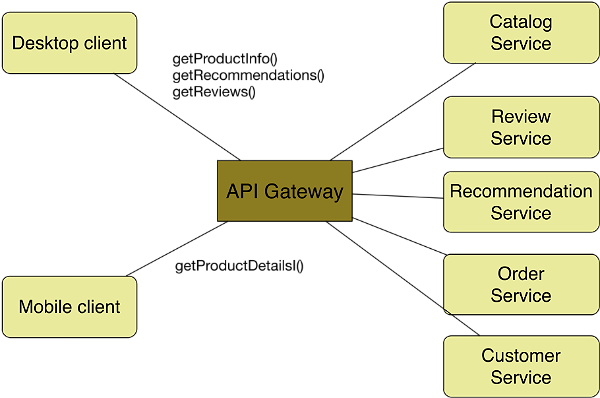
\includegraphics[width=\textwidth,height=\textheight,keepaspectratio,scale=0.1]{images/apigateway1.png}
	\caption{Architettura a microservizi e API Gateway}\label{fig:apig1}
\end{figure}
\newpage
Nella progettazione dell'architettura, il team ha seguito i vincoli posti dall'approccio architetturale \gl{REST}, i quali sono consultabili alla pagina \url{https://en.wikipedia.org/wiki/Representational_state_transfer} (visitato in data 2017-03-26).
\subsection{Sicurezza API Gateway ed endpoints}
Con lo scopo di garantire una certa sicurezza, l'accesso agli endpoints pubblicati sull'API Gateway deve essere controllato e regolato. \\Questo è necessario in quanto tramite essi è possibili fare operazioni sensibili sul sistema, quindi un utente malintenzionato potrebbe comprometterne il corretto funzionamento.\\ 
Il servizio AWS API Gateway fornisce sofisticati ed avanzati meccanismi per la protezione degli endpoint, i quali sono esposti e spiegati alla pagina \url{http://docs.aws.amazon.com/apigateway/latest/developerguide/permissions.html} (visitato in data 2017-03-26). \\

Il sistema progettato prevede due tipologie di utenti (ospite e amministratore), caratterizzati da diverse interazioni con l'assistente virtuale. Vengono quindi supportate dal \file{Back-end} differenti operazioni, invocabili tramite appositi endpoints, in base alla tipologia d'utente. Nasce di conseguenza la necessità di vincolare ogni tipologia d'utente ai soli endpoints ad essa dedicati. \\
Per soddisfare questa esigenza, non sono necessari ulteriori strumenti e meccanismi di AWS API Gateway, in quanto un amministratore è associato ad un \gl{JSON} Web Tokens (JWT) valido. Per capire quindi quali endpoints dovranno essere bloccati all'utente, sarà sufficiente controllare l'esistenza e la validità di questo JWT.
\subsection{Client}
\subsubsection{Client vocale}
L'architettura con la quale è organizzato il client vocale è quella \gl{event-driven}.\\
La motivazione che ha spinto il gruppo a prendere tale decisione è che ciò che dev'essere descritto e realizzato è facilmente modellabile utilizzando questo paradigma. Infatti, ci sono delle componenti che "aspettano" il verificarsi di un evento; altre invece che "notificano"  il verificarsi di un evento.\\
A tal fine, si è fatto utilizzo del pattern comportamentale \gl{Observer}.\\
Ad esempio, la componente \file{Recorder} (che si occupa della registrazione audio), deve prima "aspettare" che qualche individuo parli per potersi attivare, oppure deve "aspettare" che il riproduttore audio abbia terminato la riproduzione prima di potersi rimettere in ascolto.\\
Il client vocale è composto da diverse componenti, le quali sono:
\begin{itemize}
	\item \textbf{Recorder}: questa componente si occupa di realizzare le funzionalità di registrazione. Tramite la classe \file{Utility::BoolObserver}, facente parte del pattern comportamentale Observer utilizzato per modellare ciò, il registratore avrà modo di sapere se il riproduttore audio è in funzione, in maniera tale da non registrare le risposte fornite dal sistema. Una volta terminata la registrazione, il relativo audio verrà inviato alla componente \file{Logic};
	\newpage
	\item \textbf{TTS}: questa componente si occupa di realizzare le funzionalità di text-to-speech, ovvero di riprodurre sotto forma di audio il testo fornito come risposta dall'assistente virtuale. Inoltre, quando la riproduzione audio si attiva/disattiva, le componenti interessate vengono notificate di ciò. Tutto ciò è reso possibile dal pattern comportamentale Observer;
	\item \textbf{ApplicationManager}: questa componente si occupa realizzare le funzionalità di gestione delle applicazioni con le quali l'utente interagisce, permettendo la definizione di esse, la definizione comandi accettati, del salvataggio di stato e del cambio tra un'applicazione e l'altra. Tutto ciò è reso possibile dal pattern \gl{Client-side discovery} riadattato, la quale descrizione è consultabile nell'appendice \ref{CS}. Grazie all'utilizzo del pattern comportamentale Observer, questa componente viene notificata dell'arrivo di dati dal \file{Back-end};
	\item \textbf{ConversationApp}: questa componente si occupa di realizzare l'applicazione ConversationApp, ovvero quella che, tramite interfaccia utente, permette l'interazione con l'assistente virtuale. Per modellare la disposizione delle sue classi, si è fatto utilizzo del pattern Flux descritto nella libreria React, la quale verrà utilizzata per realizzare quanto appena descritto. 
	\item \textbf{Logic}: questa componente si occupa di realizzare le funzionalità che permettono l'interazione, tramite API Gateway, con il \file{Back-end}. Inoltre, quando arrivano dei dati da quest'ultimo, questa componente si occupa di notificare le componenti interessate. Ancora una volta, tutto ciò è organizzato secondo il pattern comportamentale Observer.
\end{itemize}
\subsubsection{Endpoints}
	Ora verranno definiti gli endpoints esterni utilizzati dai vari tipi di client.\\
	Per ogni risorsa sono stati specificati i formati per lo scambio dei dati in JSON:
	\begin{itemize}
		\item \textbf{Request:} rappresenta l’oggetto JSON che dovrà essere passato alla risorsa REST;
		\item \textbf{Response:} rappresenta l’oggetto JSON che fornirà in risposta la risorsa REST.
	\end{itemize}
	L'endpoint utilizzato dal client vocale è:
	\begin{itemize}
		\item \textbf{/query}\\
		\begin{itemize}
			\item \textbf{Method:} POST;
			\item \textbf{Descrizione:} invia all'API Gateway l'audio contenente la richiesta dell'utente;
			\item \textbf{Request:} la richiesta deve contenere i campi organizzati come descritto in \\\file{Back-end::APIGateway::VARequestAPIBody}:
\begin{lstlisting}[language=json,firstnumber=1]
{
 "app":"String",
 "audio":"Base64String",
 "data":"ObjectAssocArray",
 "session_id":"String"
}
\end{lstlisting}
			\item \textbf{Response:} la risposta deve contenere i campi organizzati come descritto in \\\file{Back-end::VirtualAssistant::VAResponse}:
\begin{lstlisting}[language=json,firstnumber=1]
{
"action":"String",
"res":{
 "contexts":"ObjectAssocArray",
 "data":"Object",
 "text_request":"String",
 "text_response":"String"
 },
"session_id":"String"
}
\end{lstlisting}
		\end{itemize}
	\end{itemize}

\subsection{Microservizi}
Di seguito verranno esposti e spiegati i funzionamenti di ogni microservizio da implementare.
\subsubsection{Virtual Assistant}
\paragraph{Descrizione}
Il microservizio Virtual Assistant (VA) fornisce le funzionalità di un assistente virtuale. Fa affidamento ad api.ai, e si occupa di inoltrare le richieste ricevute a tale infrastruttura. Avvalendosi di un database, permette di utilizzare diversi agenti (ciò che trasforma il linguaggio naturale in dati processabili per un'applicazione) durante la stessa interazione, consentendo quindi di definire diverse "applicazioni". Per ogni applicazione, si dovrà definire un agente.\\ Le richieste fatte all'unico endpoint di questo microservizio richiedono infatti di comunicare anche il nome dell'applicazione a cui è legata la richiesta. Questo permette di separare in diversi agenti di api.ai dialoghi legati a diverse funzionalità, affidando la realizzazione e l'integrazione di queste a diversi sviluppatori, senza dover modificare direttamente gli agenti di api.ai. \\
Per avere un completo controllo sul flusso della conversazione, si dovrà fare utilizzo di un database contenente gli agenti utilizzabili, in maniera tale che vengano usati solo quelli definiti e registrati.\\
Il microservizio si occupa anche di notificare, tramite l'utilizzo di AWS SNS, l'avvenuta interazione da parte dell'utente, permettendo così il salvataggio delle conversazioni in un database di supporto, il quale potrebbe essere utilizzato per fini di \gl{machine learning}.\\
Di seguito vengono esposti i vari passaggi affrontati all'arrivo di una richiesta:
\begin{itemize}
	\item arriva una richiesta;
	\item interrogo il database, contenente gli agenti, utilizzando il nome dell'applicazione come chiave;
	\item dall'interrogazione precedente ottengo il token dell'agente relativo all'applicazione;
	\item invio ad api.ai il token, e il testo della richiesta;
	\item api.ai fornisce la risposta, la quale viene "filtrata" da\\ \file{Back-end::VirtualAssistant::ApiAiVAAdapter::query(str: VAQuery): VAResponse}, ottenendo così un formato adatto a \file{Back-end::VirtualAssistant::VAResponse};
	\item pubblico, tramite il servizio Amazon SNS, la risposta filtrata che verrà quindi inviata al Client.
\end{itemize}
\paragraph{Endpoints}

Ora verranno definiti gli Endpoints utilizzati per i passaggi di risorse con il microservizio Virtual Assistant.\\
Per ogni risorsa sono stati specificati i formati per lo scambio dei dati in JSON:
\begin{itemize}
\item \textbf{Request:} rappresenta l’oggetto JSON che dovrà essere passato alla risorsa REST;
\item \textbf{Response:} rappresenta l’oggetto JSON che fornirà in risposta la risorsa REST.
\end{itemize}
Gli Endpoints sono:
\begin{itemize}
\item \textbf{/query}\\
\begin{itemize}
\item \textbf{Method:} POST;
\item \textbf{Descrizione:} invia al microservizio una richiesta per interrogare l'assistente virtuale;
\item \textbf{Request:} la richiesta deve contenere i campi organizzati come descritto in \\\file{Back-end::VirtualAssistant::VAQuery}:
\begin{lstlisting}[language=json,firstnumber=1]
{
 "data":"Object",
 "event":{ /*Alternativo a "text", oggetto di tipo VAEventObject*/
  "data":"Object",
  "name":"String"
 },
 "session_id":"String",
 "text":"String" /*Alternativo a "event"*/
}
\end{lstlisting}
\item \textbf{Response:} la risposta deve contenere i campi organizzati come descritto in \\\file{Back-end::VirtualAssistant::VAResponse}:
\begin{lstlisting}[language=json,firstnumber=1]
{
 "action":"String",
 "res":{/*oggetto di tipo ResponseBody*/
  "contexts":"ObjectAssocArray",
  "data":"Object",
  "text_request":"String",
  "text_response":"String"
 },
 "session_id":"String"
}
\end{lstlisting}
\end{itemize}
\end{itemize}


\subsubsection{Notifications}
\paragraph{Descrizione}
Il microservizio Notifications si occupa di mandare messaggi di notifica nei canali adeguati per notificare gli interessati dell'arrivo di un'ospite in azienda. Fornisce le API per richiedere la lista dei possibili destinatari, e per mandare il messaggio di notifica in un determinato canale. La lista dei canali viene restituita come un'array di stringhe, ognuna delle quali rappresenta un canale.\\
Il microservizio si occupa di interrogare le diverse liste fornite dalla piattaforma di messaggistica scelta e di combinarle in un'unica lista. Nel nostro caso, la piattaforma di messaggistica è \gl{Slack} e le diverse liste fornite riguardano utente, canali e gruppi privati. Quando si vuole mandare un messaggio, il campo \file{Back-end::Notifications::NotificationMessageEvent::send\_to} indica chi è il destinatario di tale messaggio.\\ \file{Back-end::Notifications::NotificationMessageEvent::msg} invece contiene il messaggio vero e proprio, nel formato definito dalla piattaforma di messaggistica su cui si appoggia il microservizio. Il formato utilizzato da Slack è consultabile alla pagina \url{https://api.slack.com/docs/message-buttons} (visitato in data 2017-03-26).
\paragraph{Endpoints}

Ora verranno definiti gli Endpoints utilizzati per i passaggi di risorse con il microservizio Notifications. \\
Per ogni risorsa sono stati specificati i formati per lo scambio dei dati in JSON:
\begin{itemize}
\item \textbf{Request:} rappresenta l’oggetto JSON che dovrà essere passato alla risorsa REST;
\item \textbf{Response:} rappresenta l’oggetto JSON che fornirà in risposta la risorsa REST.
\end{itemize}
Gli Endpoints sono:
\begin{itemize}

\item \textbf{/notifications}\\
\begin{itemize}
\item \textbf{Method:} GET;
\item \textbf{Descrizione:} restituisce la lista dei possibili canali destinatari;
\item \textbf{Response:} la risposta deve contenere i campi organizzati come descritto in \\\file{Back-end::Notifications::NotificationChannel}:
\begin{lstlisting}[language=json,firstnumber=1]
{
  "created": "String",
  "creator": "String",
  "id": "String",
  "is_archived": "boolean",
  "is_member": "boolean",
  "name": "String"
  "num_members": "int",
  "purpose": "Purpose",
  "topic": "Topic",
}
\end{lstlisting}
\end{itemize}

\begin{itemize}
\item \textbf{Method:} POST;
\item \textbf{Descrizione:} invia la notifica ad una determinata persona;
\item \textbf{Request:} la richiesta deve contenere i campi organizzati come descritto in \\\file{Back-end::Notifications::NotificationMsg}:
\begin{lstlisting}[language=json,firstnumber=1]
{
  "msg": [
	"attachments_array":[{},{}], /*Array di Back-end::Notifications::Attachment*/
	"response_type":"String",
	"text":"String"
	],
  "send_to": "String"
}
\end{lstlisting}
\end{itemize}
\end{itemize}

\subsubsection{Users}
\paragraph{Descrizione}
Il microservizio Users si occupa della gestione degli amministratori del nostro sistema. Esso fornisce delle API REST per modificare i dati relativi agli amministratori del nostro sistema presenti in un database. Viene integrato col servizio di Speech Recognition dall'API Gateway, per fornire la possibilità di effettuare il login, tramite impronta vocale, nel sistema.
\paragraph{Endpoints}

Ora verranno definiti gli Endpoints utilizzati per i passaggi di risorse con il microservizio Users. \\
Per ogni risorsa sono stati specificati i formati per lo scambio dei dati in JSON:
\begin{itemize}
\item \textbf{Request:} rappresenta l’oggetto JSON che dovrà essere passato alla risorsa REST;
\item \textbf{Response:} rappresenta l’oggetto JSON che fornirà in risposta la risorsa REST.
\end{itemize}

Gli Endpoints sono:

\begin{itemize}
\item \textbf{/auth/users}\\
\begin{itemize}
\item \textbf{Method:} GET;
\item \textbf{Descrizione:} restituisce la lista degli \file{User} presenti nel database;
\item \textbf{Response:} la risposta deve contenere un array contenente i campi organizzati come descritto in \\\file{Back-end::Auth::User}:
\begin{lstlisting}[language=json,firstnumber=1]
{
  user_array : [
  {
   "first_name":"String",
   "last_name":"String",
   "password":"String",
   "slack_channel":"String",
   "sr_id":"String",
   "username":"String"
  },
  {
   "first_name":"String",
   "last_name":"String",
   "password":"String",
   "slack_channel":"String",
   "sr_id":"String",
   "username":"String"
  },
  {
   "first_name":"String",
   "last_name":"String",
   "password":"String",
   "slack_channel":"String",
   "sr_id":"String",
   "username":"String"
  }
 ]
}
\end{lstlisting}
\end{itemize}

\begin{itemize}
\item \textbf{Method:} POST;
\item \textbf{Descrizione:} vengono inviati i dati necessari all'aggiunta di un nuovo \file{User} al database;
\item \textbf{Request:} la richiesta deve contenere i campi organizzati come descritto in\\ \file{Back-end::Auth::User}:
\begin{lstlisting}[language=json,firstnumber=1]
{
  "first_name":"String",
  "last_name":"String",
  "password":"String",
  "slack_channel":"String",
  "sr_id":"String",
  "username":"String"
}
\end{lstlisting}
\item \textbf{Response}: il corpo della risposta sarà vuoto, ma il risultato di questa operazione sarà comunque deducibile dal valore dello status code \gl{HTTP};
\end{itemize}

\item \textbf{/auth/users/:username}\\

\begin{itemize}
\item \textbf{Method:} PUT;
\item \textbf{Descrizione:} vengono modificati i dati dell'utente, il quale identificativo è specificato nel path, tramite sovrascrittura;
\item \textbf{Request:} la richiesta deve contenere i campi organizzati come descritto in \\\file{Back-end::Auth::User}
\begin{lstlisting}[language=json,firstnumber=1]
{
  "first_name":"String",
  "last_name":"String",
  "password":"String",
  "slack_channel":"String",
  "sr_id":"String",
  "username":"String"
}
\end{lstlisting}
\item \textbf{Response}: il corpo della risposta sarà vuoto, ma il risultato di questa operazione sarà comunque deducibile dal valore dello status code HTTP.
\end{itemize}

\begin{itemize}
\item \textbf{Method:} DELETE;
\item \textbf{Descrizione:} viene eliminato un utente, il quale identificativo è specificato nel path;
\item \textbf{Response}: il corpo della risposta sarà vuoto, ma il risultato di questa operazione sarà comunque deducibile dal valore dello status code HTTP;
\end{itemize}

\begin{itemize}
\item \textbf{Method:} GET;
\item \textbf{Descrizione:} vengono ricevuti i dati relativi ad un utente, il quale identificativo è specificato nel path;
\item \textbf{Response:} la risposta deve contenere i campi organizzati come descritto in \\\file{Back-end::Auth::User}:
\begin{lstlisting}[language=json,firstnumber=1]
{
  "first_name":"String",
  "last_name":"String",
  "password":"String",
  "slack_channel":"String",
  "sr_id":"String",
  "username":"String"
}
\end{lstlisting}
\end{itemize}

\end{itemize}

\subsubsection{Rules}
\paragraph{Descrizione}
Il microservizio Rules si occupa della gestione delle \gl{direttive} del sistema. Una direttiva è un'istruzione che viene data da un amministratore al sistema, la quale permette di modificare il comportamento del sistema stesso al verificarsi di certe condizioni. Tali condizioni possono essere legate alla persona che interagisce col sistema, la sua azienda di provenienza, oppure alla persona desiderata che viene richiesta.\\
Il sistema fornisce una serie di funzioni per modificare il suo comportamento, le quali indicano il modo in cui esso debba essere cambiato. \\
Una direttiva è costituita da:
\begin{itemize}
	\item una lista di target, che indica gli obiettivi (persone) ai quali deve essere applicata la direttiva;
	\item un'istanza di funzione, che indica quale delle funzioni disponibili deve essere applicata e, nel caso in cui tale funzione abbia dei parametri modificabili, con quali valori di quest'ultimi deve essere chiamata;
	\item un nome, il quale permette agli amministratori di identificare le diverse direttive;
	\item un id, il quale identifica univocamente la funzione all'interno del sistema;
	\item una flag di abilitazione, che permette di abilitare e disabilitare l'applicazione della direttiva da parte del sistema.
\end{itemize}

\paragraph{Endpoints}

Ora verranno definiti gli Endpoints utilizzati per i passaggi di risorse con il microservizio Rules.\\
Per ogni risorsa sono stati specificati i formati per lo scambio dei dati in JSON:
\begin{itemize}
\item \textbf{Request:} rappresenta l’oggetto JSON che dovrà essere passato alla risorsa REST;
\item \textbf{Response:} rappresenta l’oggetto JSON che fornirà in risposta la risorsa REST.
\end{itemize}
Gli Endpoints sono:

\begin{itemize}

\item \textbf{/impostazioni}\\

\begin{itemize}
\item \textbf{Method:} GET;
\item \textbf{Descrizione:} viene ricevuta la lista delle direttive;
\item \textbf{Response:} la risposta deve contenere un array contenente i campi organizzati come descritto in \\\file{Back-end::Rules::Rule}:
\begin{lstlisting}[language=json,firstnumber=1]
{
 rule_array : [
 {
  "ac_list":[
	"adm1":"String",
	"adm2":"String",
	...
   ],
  "ac_mode":"int",
  "enabled":"boolean",
  "id":"int",
  "name":"String",
  "targets":[ /*oggetti di tipo Back-end::Rules::RuleTarget*/
  {
   "company":"String",
   "member":"String",
   "name":"String"
  },
  {
   "company":"String",
   "member":"String",
   "name":"String"
  }
  ],
  "task":{ /* oggetto di tipo Back-end::Rules::RuleTaskInstance*/
   "params":{
	"par1":"Object",
	"par2":"Object",
	...
   }
   "task":"String"
  }
 }
 ]
}
\end{lstlisting}
\end{itemize}

\begin{itemize}
\item \textbf{Method:} POST;
\item \textbf{Descrizione:} viene creata una nuova direttiva;
\item \textbf{Request:} la richiesta deve contenere i campi organizzati come descritto in \\\file{Back-end::Rules::Rule}:
\begin{lstlisting}[language=json,firstnumber=1]
{
	rule : {
	  "ac_list":[
	    "adm1":"String",
	    "adm2":"String",
		...
	  ],
	  "ac_mode":"int",
	  "enabled":"boolean",
	  "id":"int",
	  "name":"String",
	  "targets":[ /* oggetti di tipo Back-end::Rules::RuleTarget */
	  {
		"company":"String",
		"member":"String",
		"name":"String"
      },
	  {
		"company":"String",
		"member":"String",
		"name":"String"
	  }
	  ],
	  "task":{ /* oggetto di tipo Back-end::Rules::RuleTaskInstance*/
		"params":{
		  "par1":"Object",
		  "par2":"Object",
		  ...
	   }
	  "task":"String"
	  }
	}
}
\end{lstlisting}
\item \textbf{Response}: il corpo della risposta sarà vuoto, ma il risultato di questa operazione sarà comunque deducibile dal valore dello status code HTTP;
\end{itemize}

\item \textbf{/impostazioni/:id}\\

\begin{itemize}
\item \textbf{Method:} PUT;
\item \textbf{Descrizione:} viene modificata una direttiva, il quale identificativo è specificato nel path, tramite sovrascrittura;
\item \textbf{Request:} la richiesta deve contenere i campi organizzati come descritto in \\\file{Back-end::Rules::Rule}:
\begin{lstlisting}[language=json,firstnumber=1]
{
  rule : {
	"ac_list":[
	 "adm1":"String",
	 "adm2":"String",
	...
    ],
	"ac_mode":"int",
	"enabled":"boolean",
	"id":"int",
	"name":"String",
	"targets":[ /* oggetti di tipo Back-end::Rules::RuleTarget */
	{
	 "company":"String",
	 "member":"String",
	 "name":"String"
	},
	{
	 "company":"String",
	 "member":"String",
	 "name":"String"
	}
	],
	"task":{ /* oggetto di tipo Back-end::Rules::RuleTaskInstance*/
	 "params":{
	  "par1":"Object",
	  "par2":"Object",
	  ...
	 }
	"task":"String"
   }
  }
}
\end{lstlisting}
\item \textbf{Response}: il corpo della risposta sarà vuoto, ma il risultato di questa operazione sarà comunque deducibile dal valore dello status code HTTP;
\end{itemize}

\begin{itemize}
\item \textbf{Method:} GET;
\item \textbf{Descrizione:} vengono richiesti dati relativi ad una specifica direttiva, il quale identificativo è specificato nel path;
\item \textbf{Response:} la risposta deve contenere i campi organizzati come descritto in \\\file{Back-end::Rules::Rule}:
\begin{lstlisting}[language=json,firstnumber=1]
{
	rule : {
	 "ac_list":[
	  "adm1":"String",
	  "adm2":"String",
	  ...
	  ],
	"ac_mode":"int",
	"enabled":"boolean",
	"id":"int",
	"name":"String",
	"targets":[ /* oggetti di tipo Back-end::Rules::RuleTarget */
	{
	 "company":"String",
	 "member":"String",
	 "name":"String"
	},
	{
	 "company":"String",
	 "member":"String",
	 "name":"String"
	}
	],
	"task":{ /* oggetto di tipo Back-end::Rules::RuleTaskInstance*/
	 "params":{
	  "par1":"Object",
	  "par2":"Object",
	  ...
	 }
	"task":"String"
	}
  }
}
\end{lstlisting}

\end{itemize}

\begin{itemize}
\item \textbf{Method:} DELETE;
\item \textbf{Descrizione:} viene eliminata una direttiva, il quale identificativo è specificato nel path;
\item \textbf{Response}: il corpo della risposta sarà vuoto, ma il risultato di questa operazione sarà comunque deducibile dal valore dello status code HTTP;
\end{itemize}


\item \textbf{/impostazioni/tasks}\\

\begin{itemize}
\item \textbf{Method:} GET;
\item \textbf{Descrizione:} viene richiesta la lista dei tipi di funzioni presenti nel sistema;
\item \textbf{Response:} la risposta deve contenere i campi organizzati come descritto in \\\file{Back-end::Rules::Task}:
\begin{lstlisting}[language=json,firstnumber=1]
{
 function_array : [
 {
  "function":"String",
  "id":"int"
 },
 {
  "function":"String",
  "id":"int"
 }
]
}
\end{lstlisting}
\end{itemize}

\begin{itemize}
\item \textbf{Method:} POST;
\item \textbf{Descrizione:} viene creato un nuovo tipo di \file{Task};
\item \textbf{Request:} la richiesta deve contenere i campi organizzati come descritto in \\\file{Back-end::Rules::Task}:
\begin{lstlisting}[language=json,firstnumber=1]
{
 function_array : [
 {
  "function":"String",
  "id":"int"
 },
 {
  "function":"String",
  "id":"int"
 }
 ]
}
\end{lstlisting}
\item \textbf{Response}: il corpo della risposta sarà vuoto, ma il risultato di questa operazione sarà comunque deducibile dal valore dello status code HTTP.
\end{itemize}



\item \textbf{/impostazioni/tasks/:type}\\

\begin{itemize}
\item \textbf{Method:} GET;
\item \textbf{Descrizione:} viene richiesto un \file{Task} in base al tipo di funzione applicata, , il quale identificativo è specificato nel path;

\item \textbf{Response:} la risposta deve contenere i campi organizzati come descritto in \\\file{Back-end::Rules::Task}:
\begin{lstlisting}[language=json,firstnumber=1]
{
 function_array : [
 {
  "function":"String",
  "id":"int"
 },
 {
  "function":"String",
  "id":"int"
 }
 ]
}
\end{lstlisting}
\end{itemize}

\begin{itemize}
\item \textbf{Method:} PUT;
\item \textbf{Descrizione:} viene modificata un \file{Task}, il quale identificativo è specificato nel path tramite sovrascrittura;
\item \textbf{Request:} la richiesta deve contenere i campi organizzati come descritto in \\\file{Back-end::Rules::Task}:
\begin{lstlisting}[language=json,firstnumber=1]
{
 function_array : [
 {
  "function":"String",
  "id":"int"
 },
 {
  "function":"String",
  "id":"int"
 }
 ]
}
\end{lstlisting}
\item \textbf{Response}: il corpo della risposta sarà vuoto, ma il risultato di questa operazione sarà comunque deducibile dal valore dello status code HTTP.
\end{itemize}

\end{itemize}
\newpage
\subsection{Action supportate} \label{action}
Di seguito vengono elencate le action, supportate dal \file{Back-end}, che api.ai può ritornare in seguito alla richiesta di un utente. \\
Una action è una stringa che indica quale operazione dovrà essere scelta dall'API Gateway, in modo da soddisfare le richieste dell'utente.\\
I metodi citati appartengono alla classe \file{Back-end::APIGateway::VocalAPI}.
\subsubsection{User}
\begin{itemize}
\item \file{user.add}: utilizza il metodo privato \file{addUser(user: User)} per aggiungere un utente registrato, cioè un amministratore, al sistema;

\item \file{user.get}: utilizza il metodo privato \file{getUser(username: String)} per ottenere i dati relativi ad un utente registrato;

\item \file{user.getList}: utilizza il metodo privato \file{getUserList()} per ottenere la lista degli utenti registrati; 

\item \file{user.update}: utilizza il metodo privato \file{updateUser(user: User)} per aggiornare un utente registrato;

\item \file{user.remove}: utilizza il metodo privato \file{removeUser(username: String)} per rimuovere un utente registrato;

\item \file{user.addEnrollment}: utilizza il metodo privato \file{addUserEnrollment(enr: Enrollment)} per aggiungere un Enrollment ad un utente registrato;

\item \file{user.resetEnrollments}: utilizza il metodo privato \file{resetUserEnrollment(username: String):} per resettare gli Enrollment relativi ad un utente registrato;

\item \file{user.login}: utilizza il metodo privato \file{loginUser(enr: Enrollment)} per effettura il login di un utente registrato.

\end{itemize}
\subsubsection{Rule}
\begin{itemize}
\item \file{rule.add}: utilizza il metodo privato \file{addRule(rule: Rule)} per aggiungere una direttiva;

\item \file{rule.get}: utilizza il metodo privato \file{getRule(id: String)} per ottenere i dati relativi una direttiva;

\item \file{rule.getList}: utilizza il metodo privato \file{getRuleList()} per ottenere la lista delle direttive;

\item \file{rule.update}: utilizza il metodo privato \file{updateRule(rule: Rule)} per aggiornare una direttiva;

\item \file{rule.remove}: utilizza il metodo privato \file{removeRule(id: String)} per rimuovere una direttiva.


\end{itemize}

\section{Diagrammi riassuntivi dei \gl{package}}
Di seguito sono riportati tutti i package dell’applicativo per chiarire la relazione tra le componenti e le classi al suo interno. Per chiarezza ed esigenza di spazio le classi rappresentate all’interno dei package sono rappresentate senza metodi e attributi.


\subsection{Back-end}
\gl{Package} contenente tutte le componenti che costituiscono il back-end. Le componenti sono organizzate secondo il pattern a \gl{microservizi}.
\begin{figure}[h] \centering 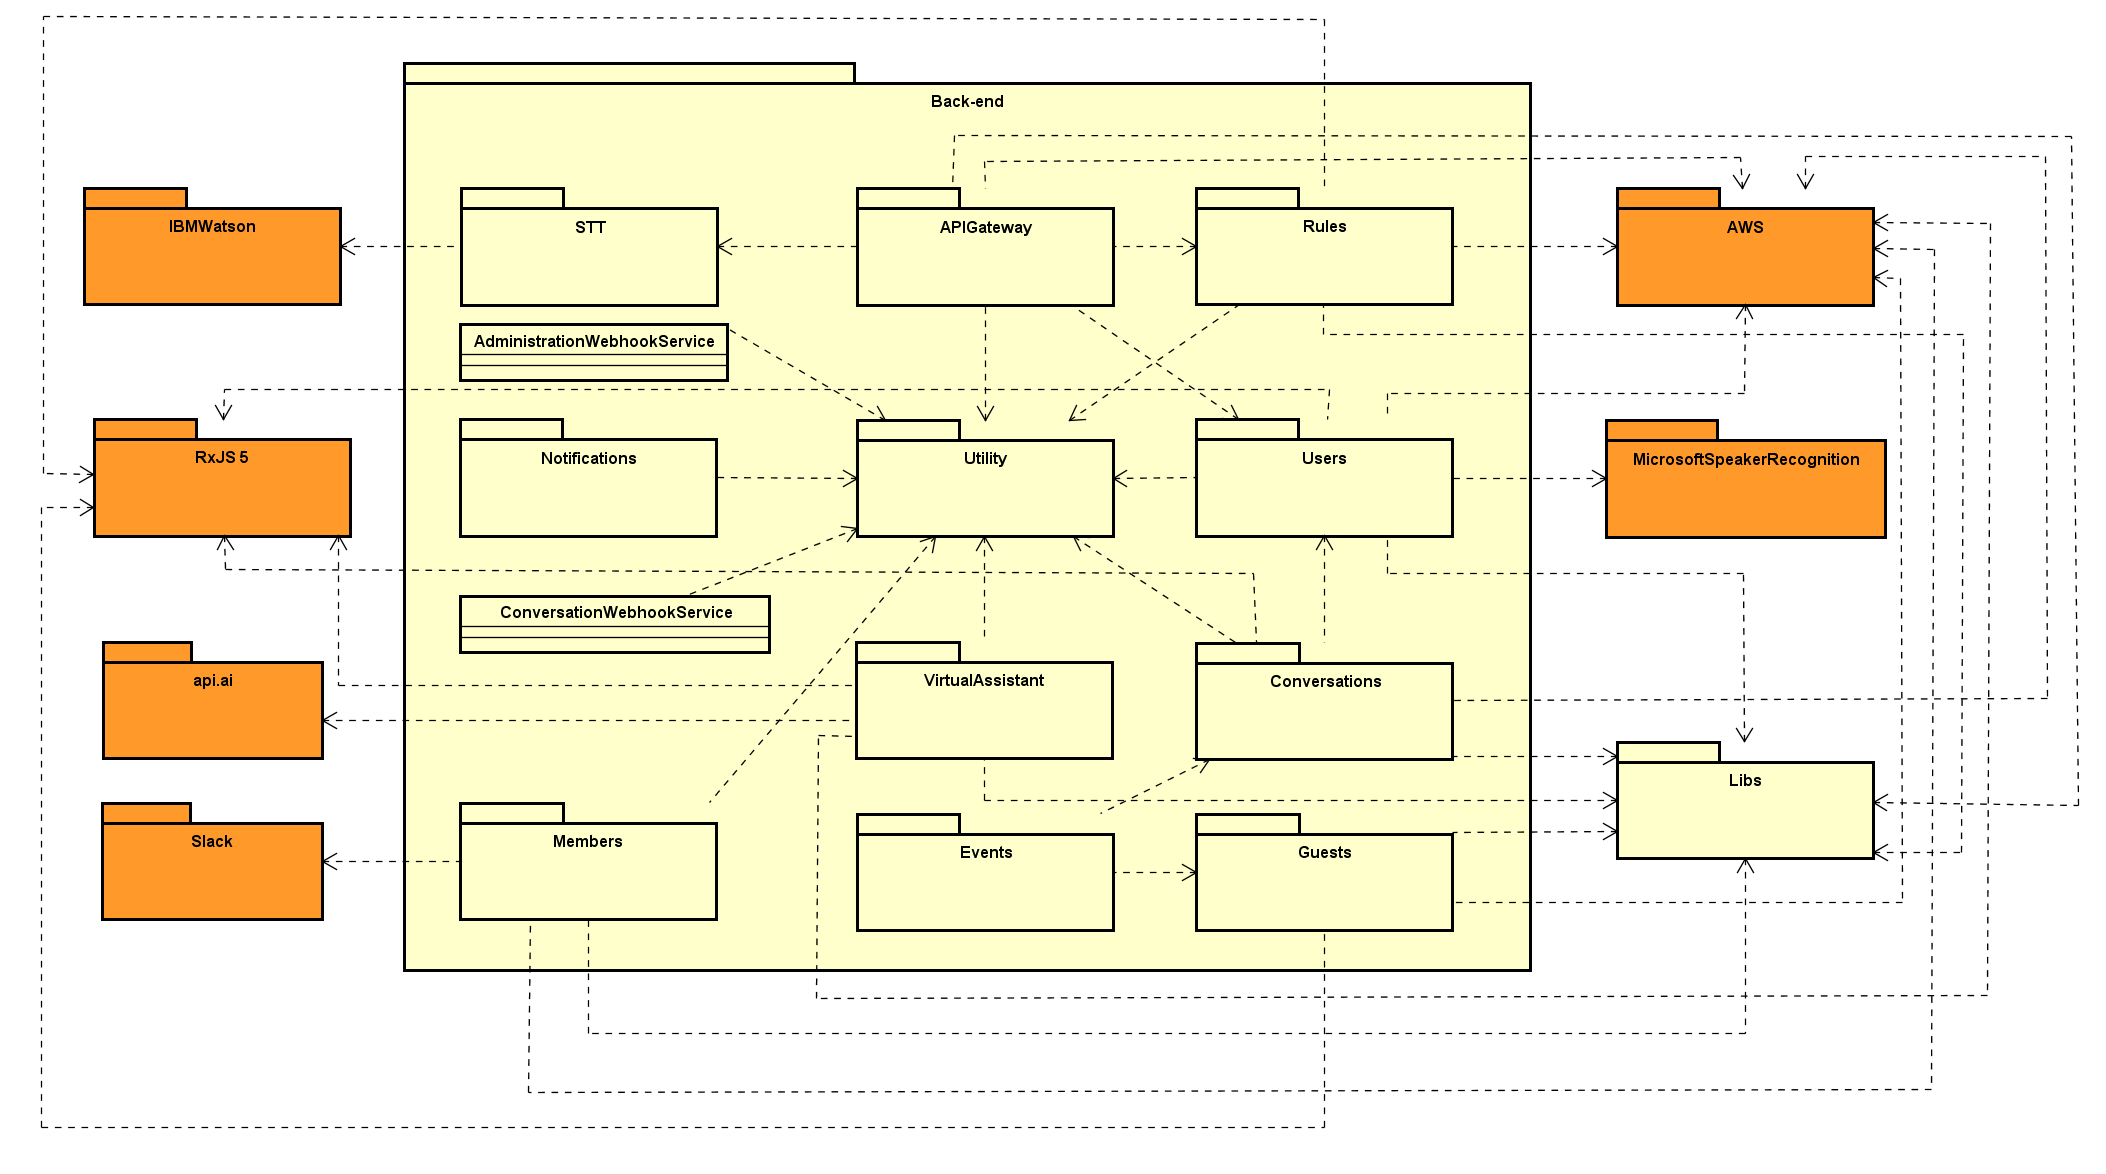
\includegraphics[width=\textwidth,height=\textheight,keepaspectratio]{images/diagrams/back-end/Official_Backend_0304/Back-end.png}
	\caption{Package Back-end}
\end{figure}
\newpage

\subsection{Back-end::\gl{API}\gl{Gateway}}
In questo package sono contenute le classi che realizzano:
\begin{itemize}
	\item le funzionalità da \gl{API Gateway}, permettendo l'interazione \file{Client} - \file{Back-end} tramite la pubblicazione di appositi \gl{endpoint};
	\item la mappatura delle richieste del \file{Client} nelle funzionalità supportate dal \file{Back-end};
	\item la conversione di un audio nel formato accettato dai servizi esterni utilizzati;
	\item la pubblicazione sul topic SNS per notificare la persona desiderata e segnalare la necessità di registrare l'interazione appena avvenuta con l'interlocutore;
	\item il login tramite impronta vocale.
\end{itemize}
\begin{figure}[h] \centering 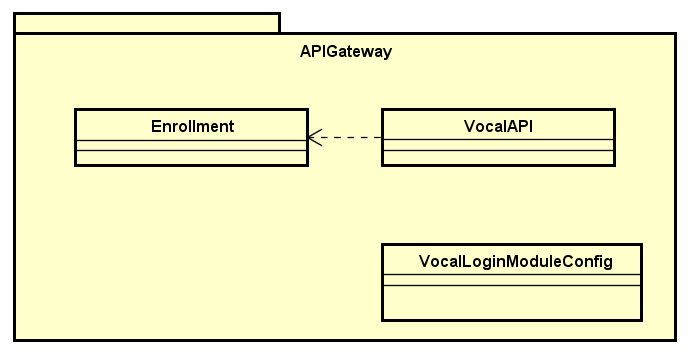
\includegraphics[width=\textwidth,height=\textheight,keepaspectratio]{images/diagrams/back-end/Official_Backend_0304/APIGateway.png}
	\caption{Package Back-end::APIGateway}
\end{figure}
\newpage



\subsection{Back-end::Conversations}
In questo package sono contenute le classi che realizzano: \begin{itemize} \item la definizione di una conversazione e dei messaggi contenuti in essa; \item l'interfaccia per l'interazione con il database contenente le conversazioni sostenute; \item le modalità con le quali i dati devono essere trasmessi dal e al database. \end{itemize}
\begin{figure}[h] \centering 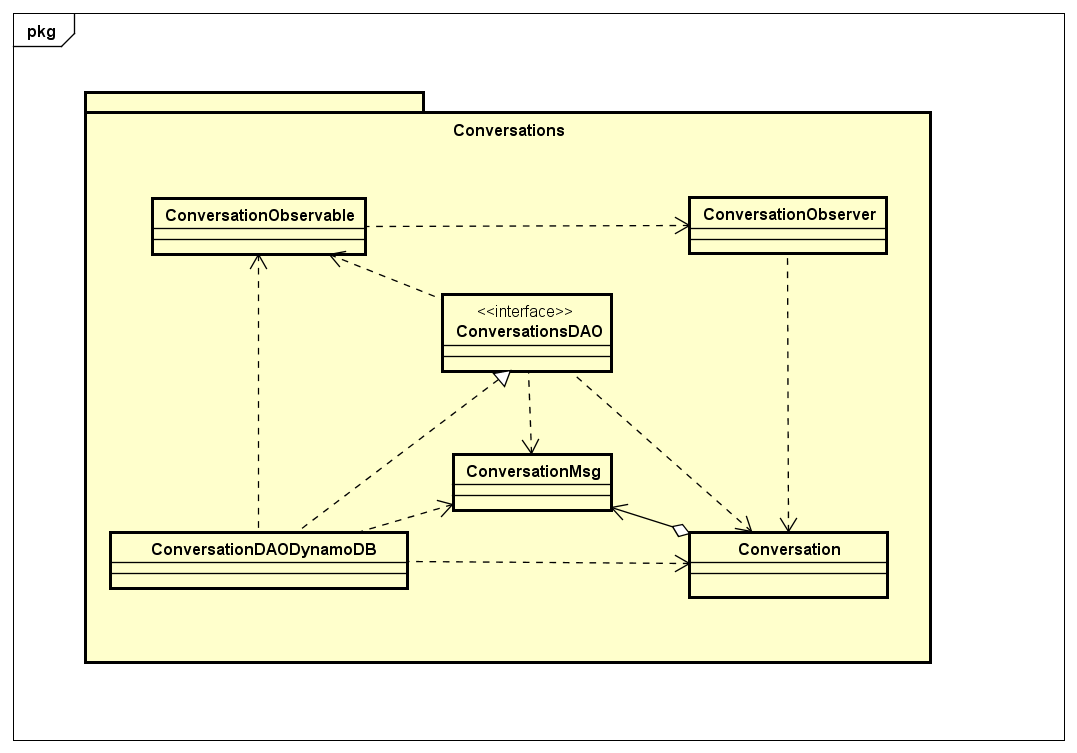
\includegraphics[width=\textwidth,height=\textheight,keepaspectratio]{images/diagrams/back-end/Official_Backend_0304/Conversations.png}
	\caption{Package Back-end::Conversations}
\end{figure}
\newpage

\subsection{Back-end::Events}
In questo package sono contenute le classi che realizzano: \begin{itemize} \item la definizione dei messaggi che devono essere pubblicati sul topic SNS dal quale verranno generati degli eventi; \item la definizione dei dati che le lambda function, innescate da questi eventi, devono processare; \item l'invio di una notifica alla persona desiderata e il salvataggio dell'interazione avvenuta con il \gl{sistema} da parte dell'interlocutore. \end{itemize}
\begin{figure}[h] \centering 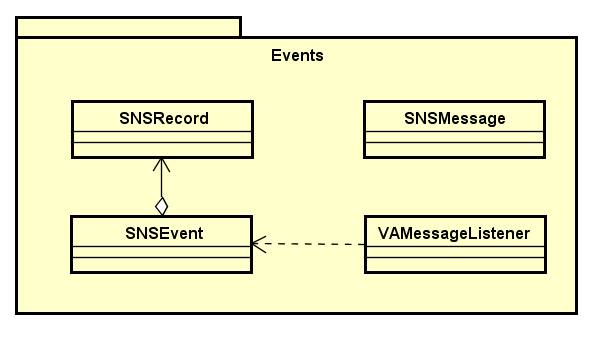
\includegraphics[width=\textwidth,height=\textheight,keepaspectratio]{images/diagrams/back-end/Official_Backend_0304/Events.png}
	\caption{Package Back-end::Events}
\end{figure}
\newpage

\subsection{Back-end::Guests}
In questo package sono contenute le classi che realizzano: \begin{itemize} \item la definizione dei dati associati ad un ospite che ha interagito con il sistema; \item l'interfaccia per l'interazione con il database contenente gli ospiti conosciuti; \item le modalità con le quali i dati devono essere trasmessi dal e al database. \end{itemize}	
\begin{figure}[h] \centering 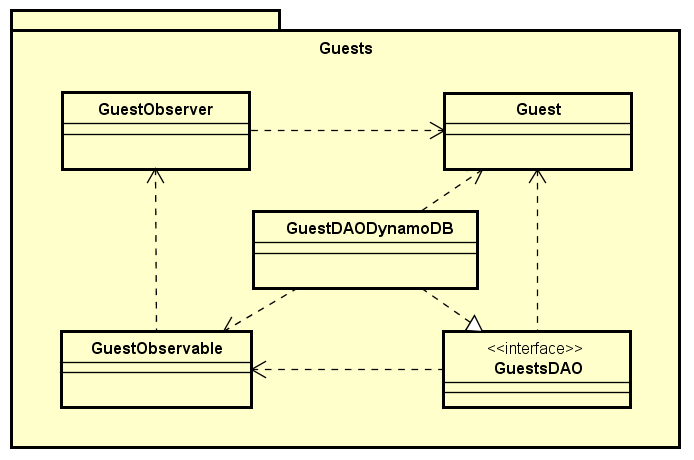
\includegraphics[width=\textwidth,height=\textheight,keepaspectratio]{images/diagrams/back-end/Official_Backend_0304/Guest.png}
	\caption{Package Back-end::Guests}
\end{figure}
\newpage

\subsection{Back-end::Members}
In questo package sono contenute le classi che realizzano: \begin{itemize} \item la definizione dei dati associati ad un membro dell'azienda al quale indirizzare una \gl{direttiva}; \item l'interfaccia per l'interazione con il database contenente i membri dell'azienda; \item le modalità con le quali i dati devono essere trasmessi dal e al database. \end{itemize}
\begin{figure}[h] \centering 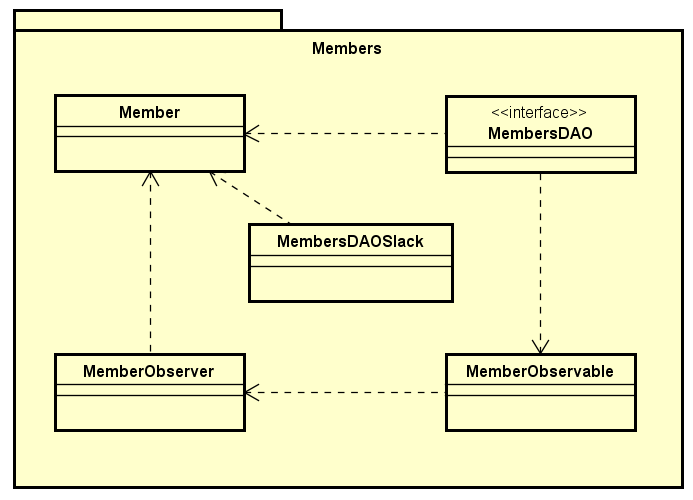
\includegraphics[width=\textwidth,height=\textheight,keepaspectratio]{images/diagrams/back-end/Official_Backend_0304/Member.png}
	\caption{Package Back-end::Members}
\end{figure}
\newpage

\subsection{Back-end::Notifications}
Package contenente le classi e le interfacce che realizzano il \gl{microservizio} relativo alla gestione delle notifiche da inviare alla persona desiderata su una certa piattaforma di messaggistica.\\ Sono contenute le classi che realizzano: \begin{itemize} \item la definizione dei dati di un messaggio da inviare alla persona desiderata; \item la definizione dei dati del canale associato alla persona desiderata; \item il microservizio che espone gli endpoint per permetterne il suo utilizzo. \end{itemize}
\begin{figure}[h] \centering 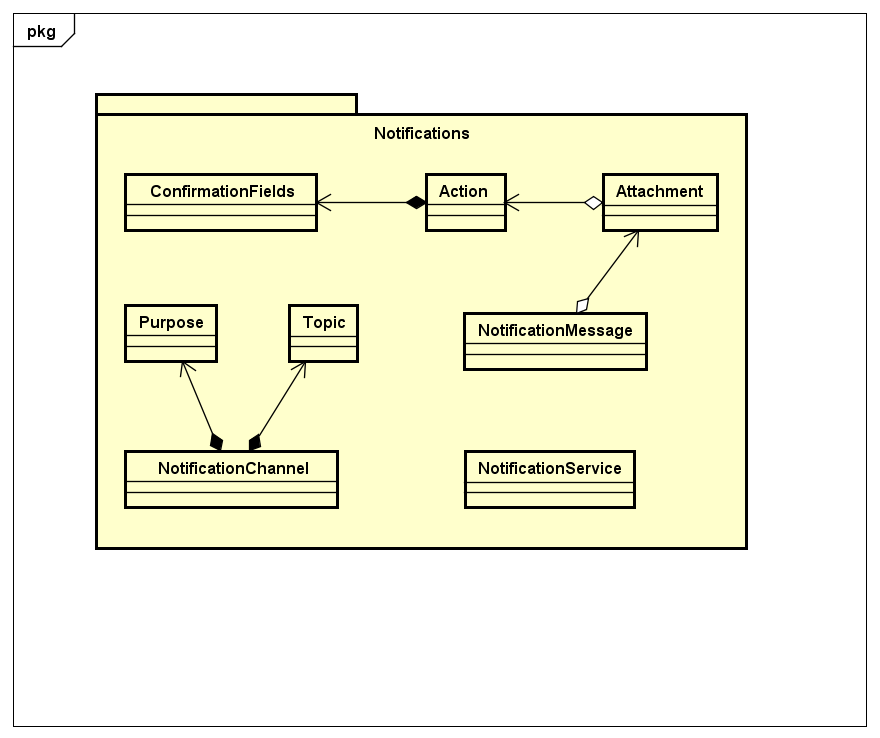
\includegraphics[width=\textwidth,height=\textheight,keepaspectratio]{images/diagrams/back-end/Official_Backend_0304/Notifications.png}
	\caption{Package Back-end::Notifications}
\end{figure}
\newpage

\subsection{Back-end::Rules}
Package contenente le classi e le interfacce che realizzano il microservizio di gestione delle \gl{direttive} per l'assistente virtuale.\\ Vengono offerte funzionalità che permettono: \begin{itemize} \item l'aggiunta di una nuova direttiva; \item l'aggiunta di un nuovo compito (\file{\gl{Task}}) che una direttiva deve eseguire; \item la gestione delle direttive esistenti; \item la gestione dei compiti esistenti. \end{itemize} Sono contenute le classi che realizzano: \begin{itemize} \item la definizione dei dati di una direttiva; \item l'interfaccia per l'interazione con il database contenente le direttive; \item la definizione dei dati di un \gl{task}; \item l'interfaccia per l'interazione con il database contenente i task; \item le modalità con le quali i dati devono essere trasmessi dai e ai database; \item il microservizio che espone gli endpoint per permetterne il suo utilizzo. \end{itemize}
\begin{figure}[h] \centering 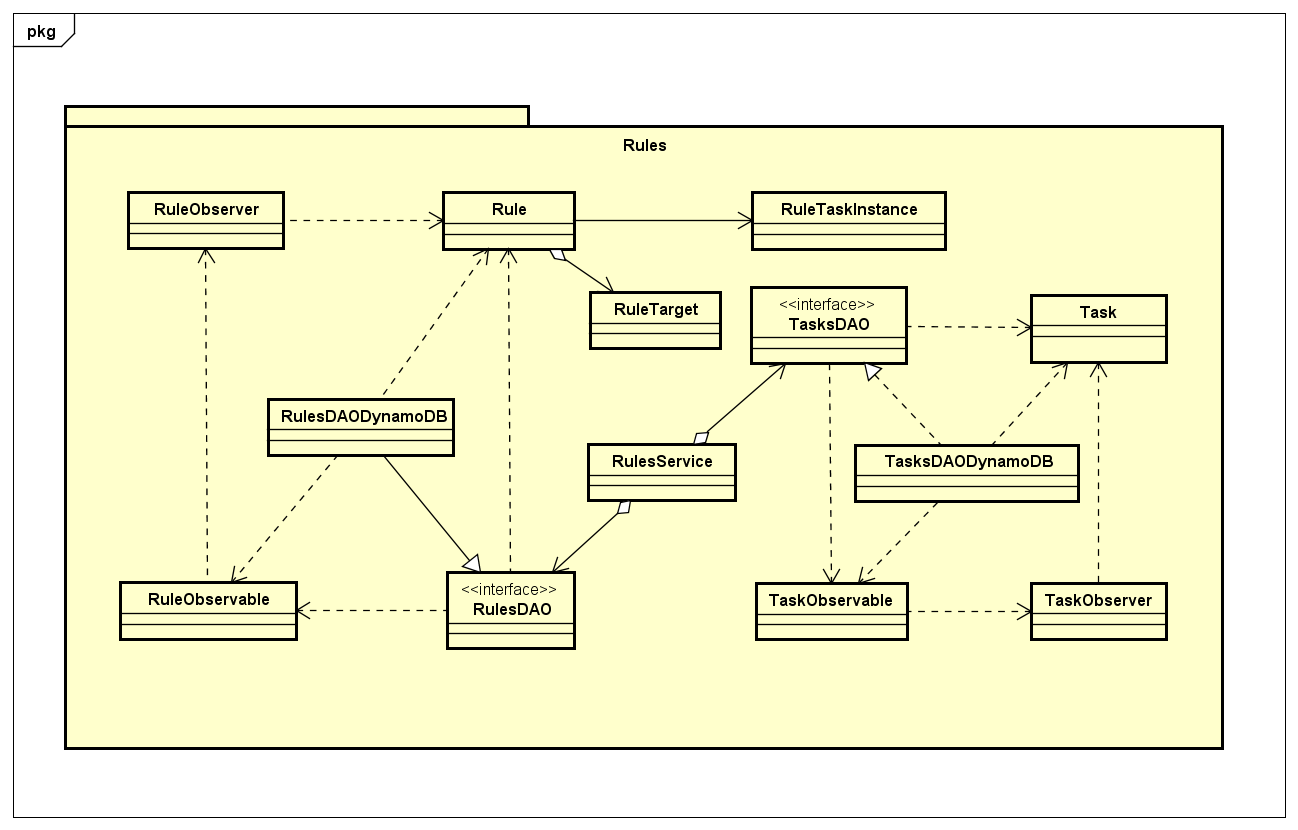
\includegraphics[width=\textwidth,height=\textheight,keepaspectratio]{images/diagrams/back-end/Official_Backend_0304/Rules.png}
	\caption{Package Back-end::Rules}
\end{figure}
\newpage

\subsection{Back-end::STT}
Package che include le classi che si occupano di fornire le funzionalità di \gl{Speech to text}.\\ Le classi contenute realizzano: \begin{itemize} \item l'interfaccia e le modalità di utilizzo del servizio esterno di Speech to Text. \end{itemize}
\begin{figure}[h] \centering 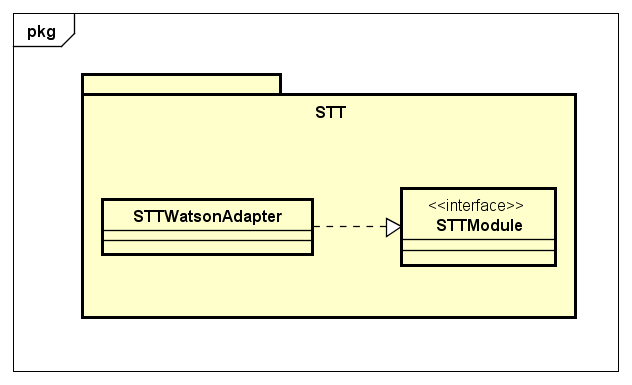
\includegraphics[width=\textwidth,height=\textheight,keepaspectratio]{images/diagrams/back-end/Official_Backend_0304/STT.png}
	\caption{Package Back-end::STT}
\end{figure}
\newpage

\subsection{Back-end::Users}
Package contenente le classi e le interfacce che realizzano il microservizio di autenticazione e registrazione di un amministratore nel sistema.\\ Vengono offerte funzionalità che permettono: \begin{itemize} \item la registrazione di un nuovo amministratore; \item l'autenticazione di un amministratore; \item gestione degli amministratori esistenti. \end{itemize} Sono contenute le classi che realizzano: \begin{itemize} \item la definizione dei dati di un utente registrato; \item l'interfaccia per l'interazione con il database contenente gli utenti registrati; \item le modalità con le quali i dati devono essere trasmessi dal e al database; \item le modalità di interazione che il servizio esterno di riconoscimento vocale; \item il microservizio che espone gli endpoint per permetterne il suo utilizzo. \end{itemize}
\begin{figure}[h] \centering 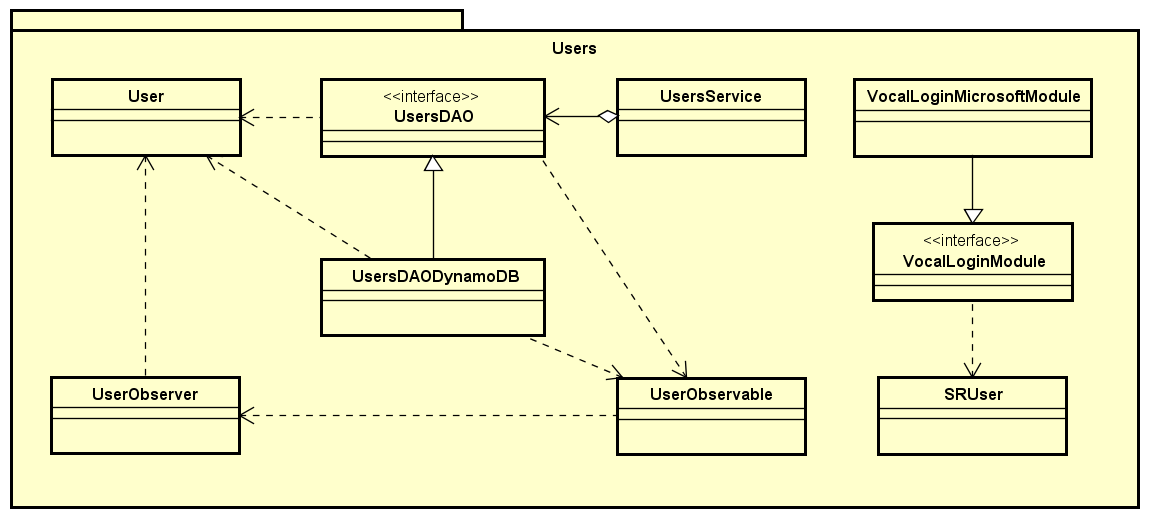
\includegraphics[width=\textwidth,height=\textheight,keepaspectratio]{images/diagrams/back-end/Official_Backend_0304/Users.png}
	\caption{Package Back-end::Users}
\end{figure}
\newpage

\subsection{Back-end::Utility}
Package contenente classi e interfacce, dallo scopo generico, utili ad altri package del back-end
\begin{figure}[h] \centering 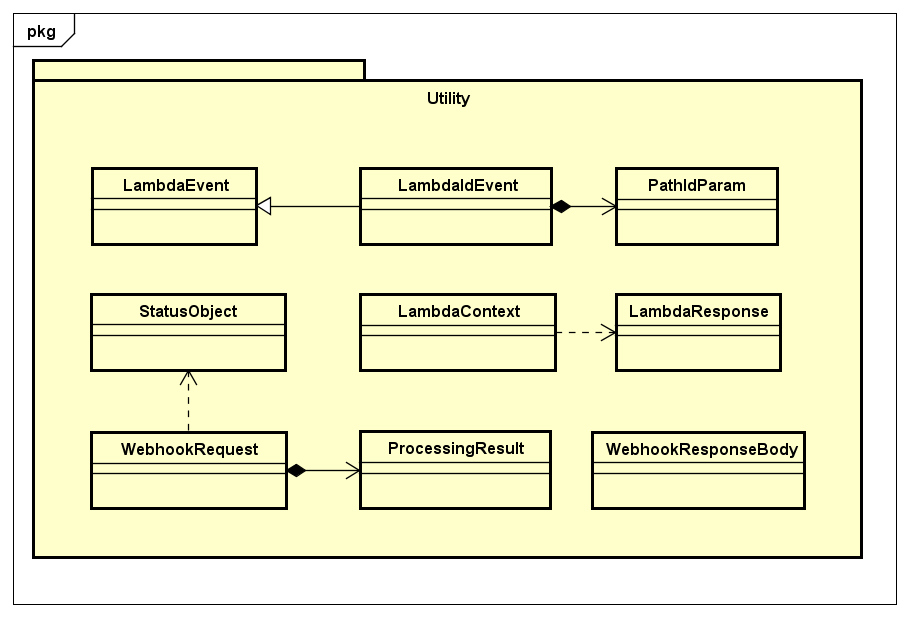
\includegraphics[width=\textwidth,height=\textheight,keepaspectratio]{images/diagrams/back-end/Official_Backend_0304/Utility.png}
	\caption{Package Back-end::Utility}
\end{figure}
\newpage

\subsection{Back-end::VirtualAssistant}
Package contenente le classi e le interfacce che realizzano il microservizio di assistente virtuale .\\ Vengono offerte funzionalità che permettono di: \begin{itemize} \item interrogare l'assistemte virtuale. \end{itemize} Sono contenute le classi che realizzano: \begin{itemize} \item la definizione dei dati di un agent; \item l'interfaccia per l'interazione con il database contenente gli agent; \item le modalità con le quali i dati devono essere trasmessi dal e al database; \item la definizione dei dati da scambiare con i \gl{webhook}; \item l'interfaccia e le modalità di interazione con il servizio esterno di assistente virtuale (api.ai); \item il microservizio che espone gli endpoint per permetterne il suo utilizzo. \end{itemize}
\begin{figure}[h] \centering 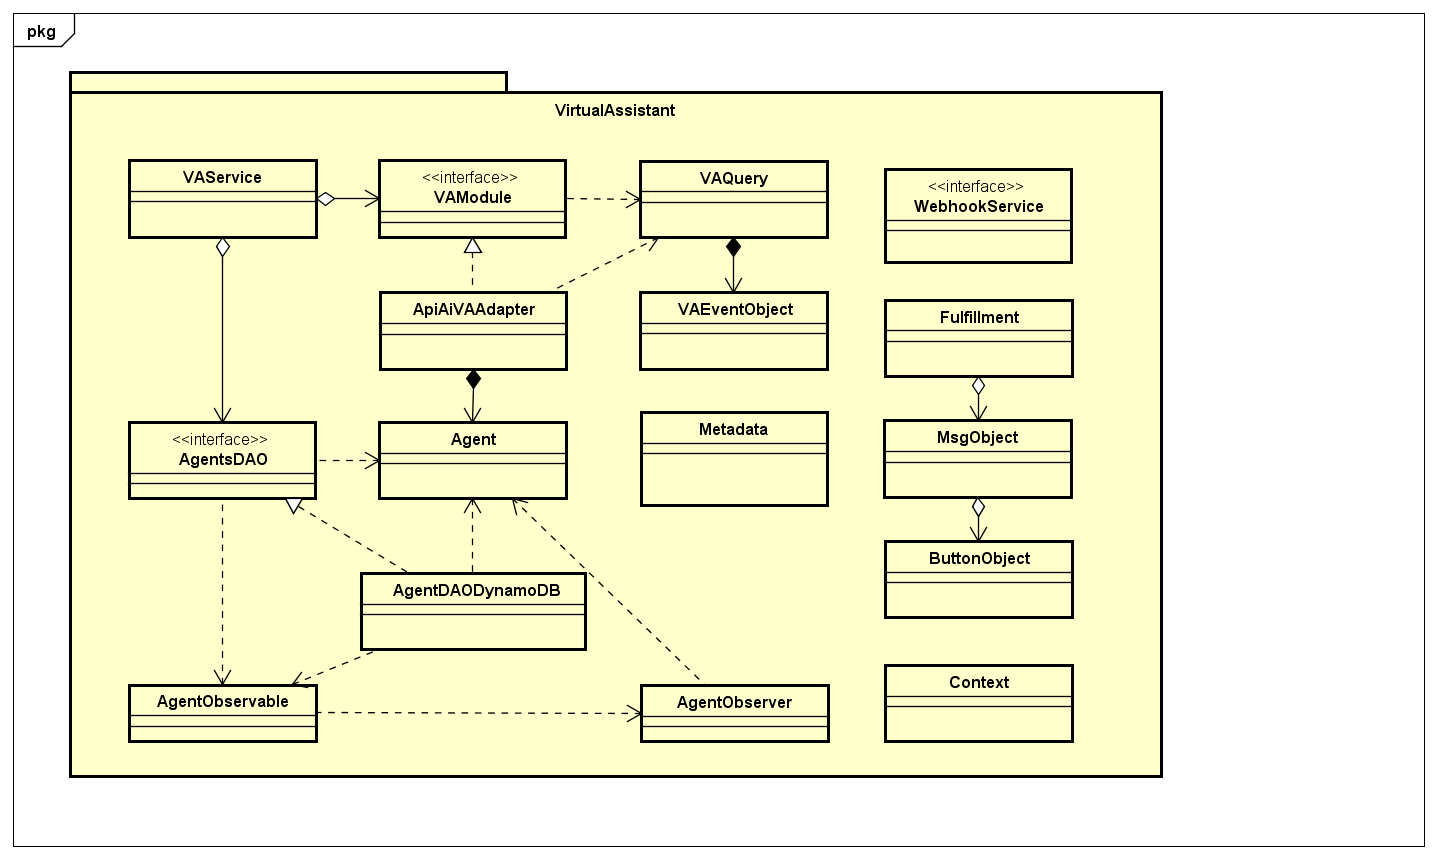
\includegraphics[width=\textwidth,height=\textheight,keepaspectratio]{images/diagrams/back-end/Official_Backend_0304/VirtualAssistant.png}
	\caption{Package Back-end::VirtualAssistant}
\end{figure}
\newpage

\subsection{Client}
Package che racchiude tutte le componenti del client. Il pattern utilizzato per organizzare le componenti è quello di un'architettura \gl{event-driven}.
\begin{figure}[h] \centering 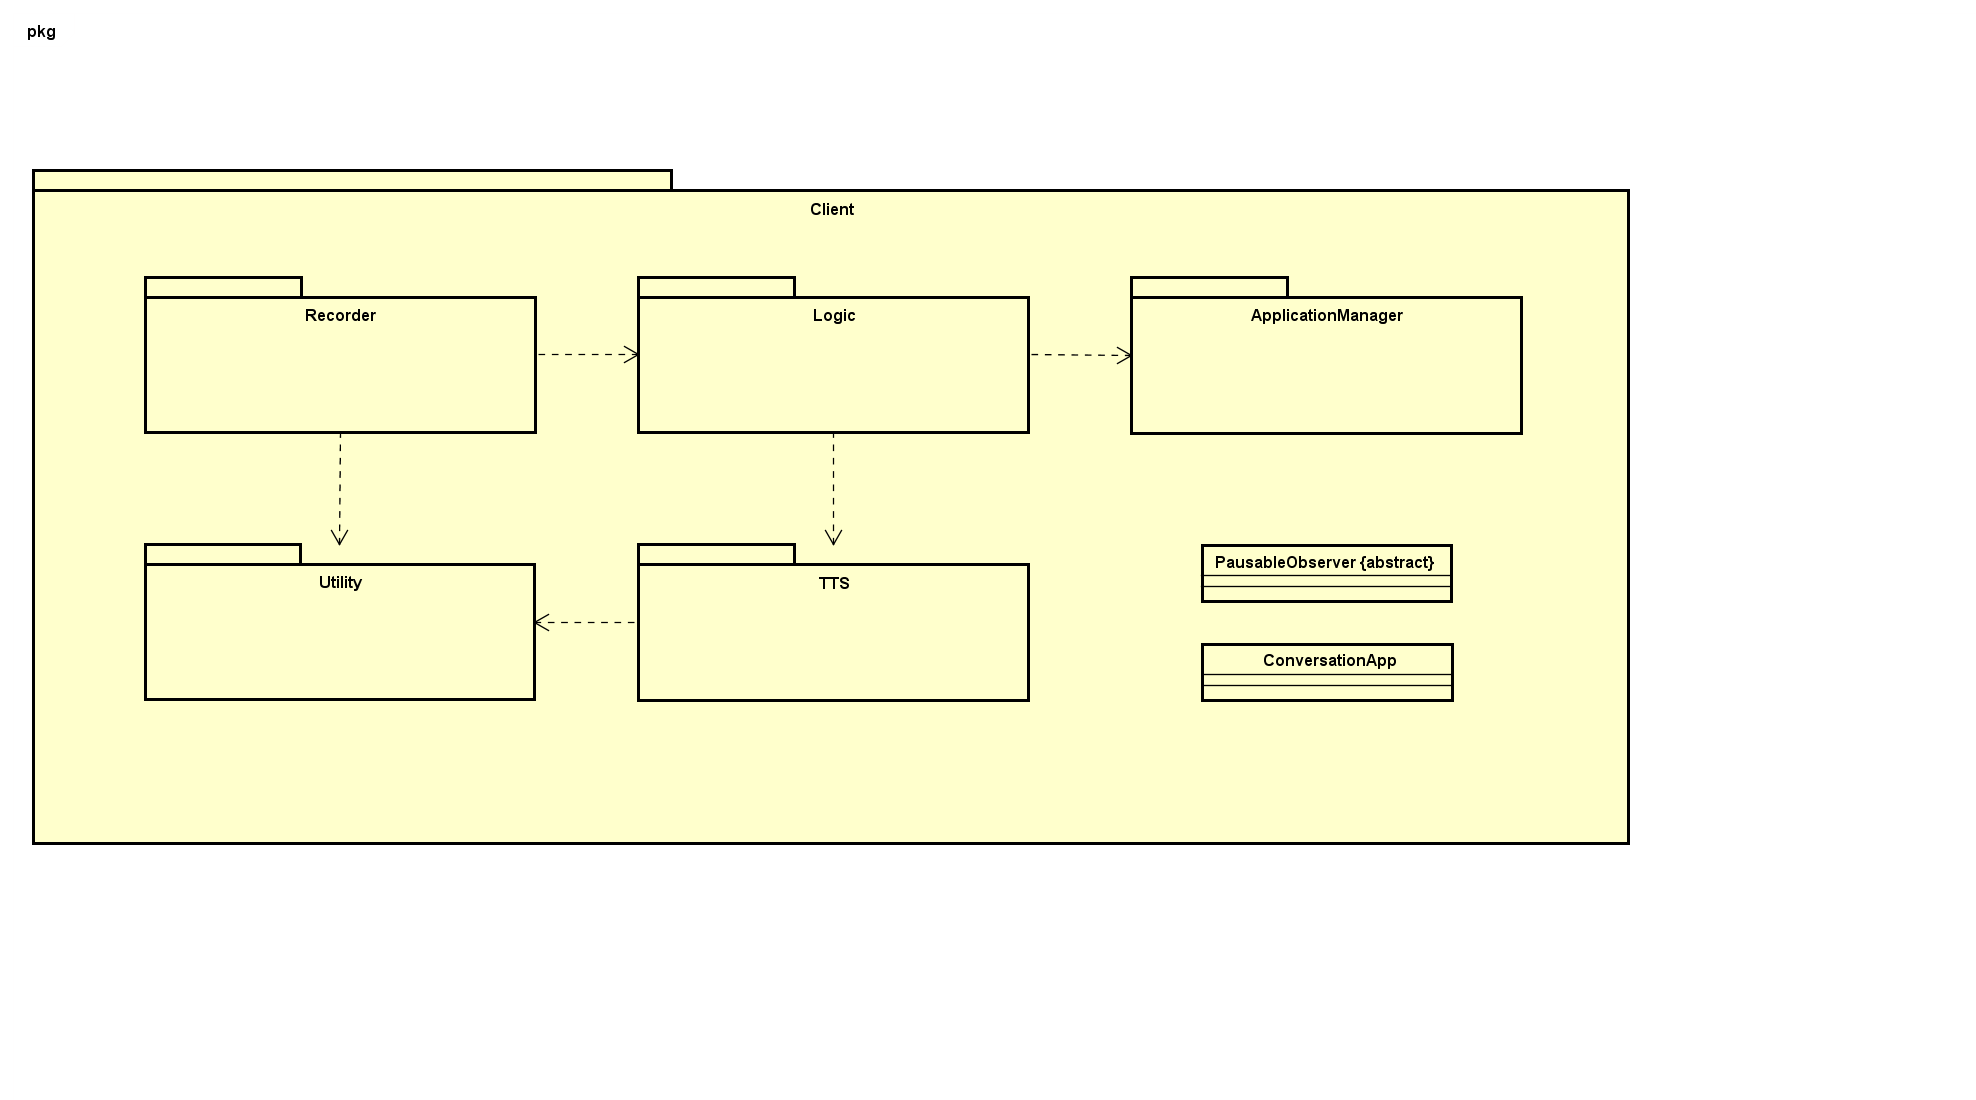
\includegraphics[width=\textwidth,height=\textheight,keepaspectratio]{images/diagrams/client/Client/Client.png}
	\caption{Package Client}
\end{figure}
\newpage


\subsection{Client::ApplicationManager}
Package contenente le classi che si occupano della gestione delle applicazioni con le quali l'utente può interagire.\\ Vengono offerte funzionalità che permettono: \begin{itemize} \item la reazione a dei dati di risposta arrivati dal \file{Back-end}; \item la definizione di ciò che va a comporre una applicazione; \item il salvataggio dello stato di un'applicazione; \item il cambio di un'applicazione con un'altra. \end{itemize}
\begin{figure}[h] \centering 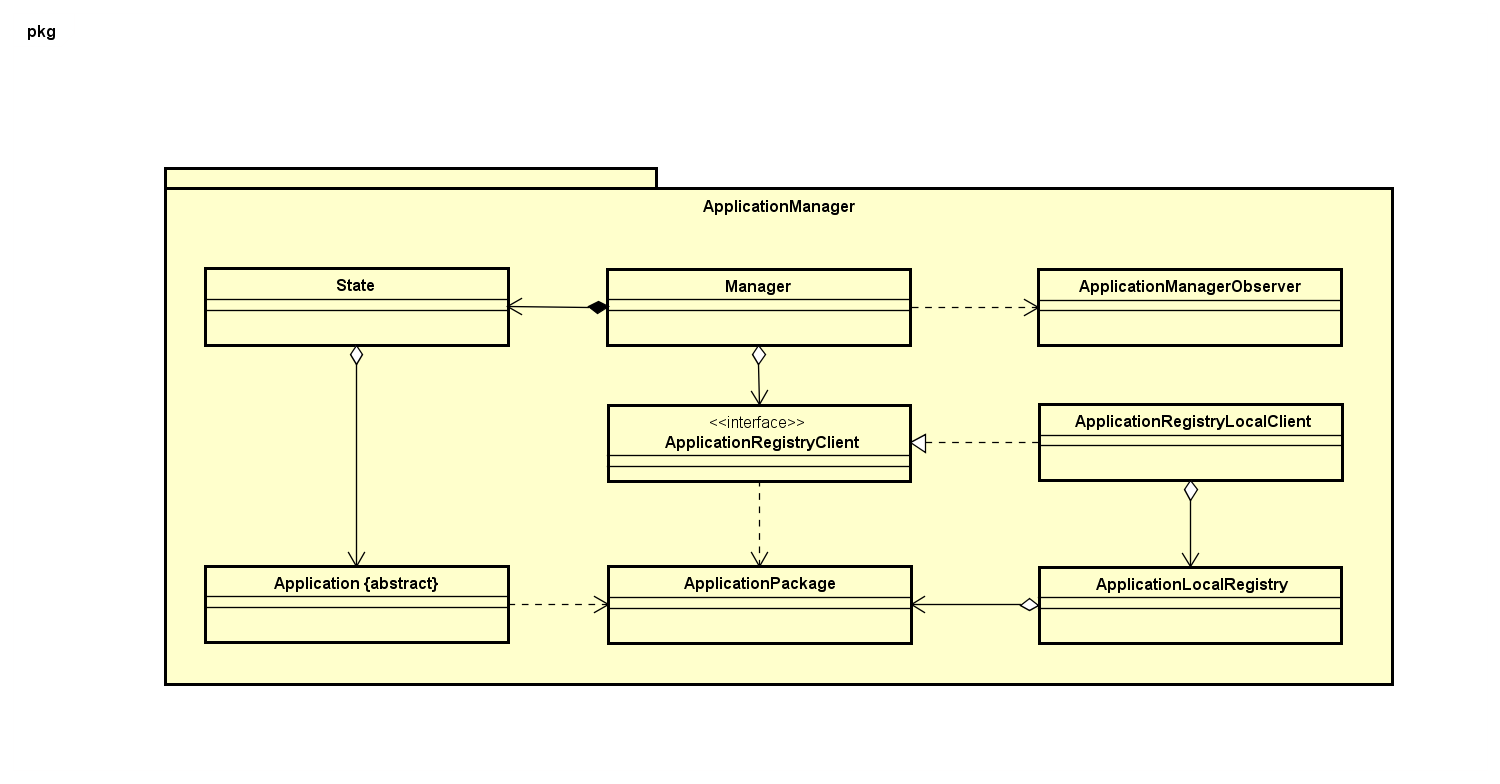
\includegraphics[width=\textwidth,height=\textheight,keepaspectratio]{images/diagrams/client/Client/ApplicationManager.png}
	\caption{Package Client::ApplicationManager}
\end{figure}
\newpage

\subsection{Client::ConversationApp}
In questo package è definita l'applicazione di conversazione, la quale fornisce un'interfaccia utente per l'interazione con l'assistente virtuale.\\ Le classi contenute in questo package permettono di: \begin{itemize} \item tenere traccia delle conversazioni effettuate con gli ospiti; \item notificare gli observer collegati che è stata decisa la \file{ConversationAction}; \item gestire i comandi da eseguire da \file{ConversationApp}. \end{itemize}
\begin{figure}[h] \centering 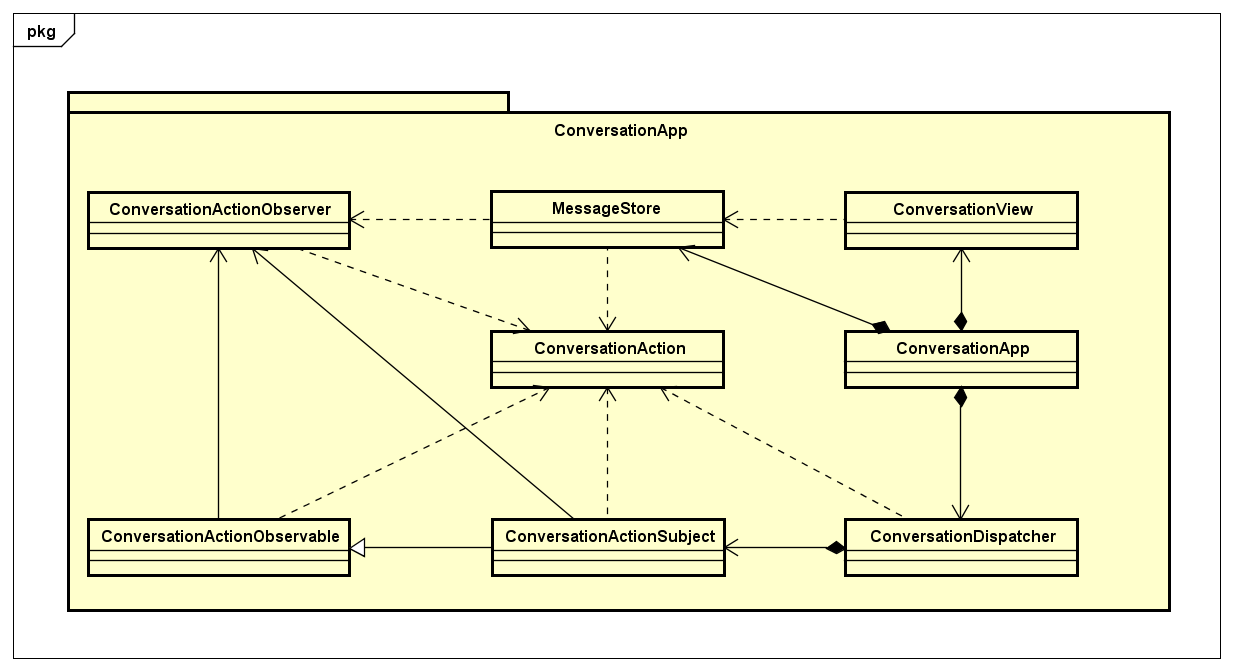
\includegraphics[width=\textwidth,height=\textheight,keepaspectratio]{images/diagrams/client/Client/ConversationApp.png}
	\caption{Package Client::ConversationApp}
\end{figure}
\newpage

\subsection{Client::Logic}
Package contenente le classi che gestiscono la logica del client e che si occupano della comunicazione con il back-end.\\ Le classi contenute permettono : \begin{itemize} \item l'esecuzione una determinata azione in base ai dati arrivati come richiesta dal registratore vocale; \item il notificare alle classi interessate l'arrivo del testo di risposta dal \file{Back-end}; \item l'esecuzione di richieste \gl{HTTP} sostituendo le funzioni di \gl{Callback} fornite da Javascript con le Promise che sono più chiare in casi di annidamento; \end{itemize}
\begin{figure}[h] \centering 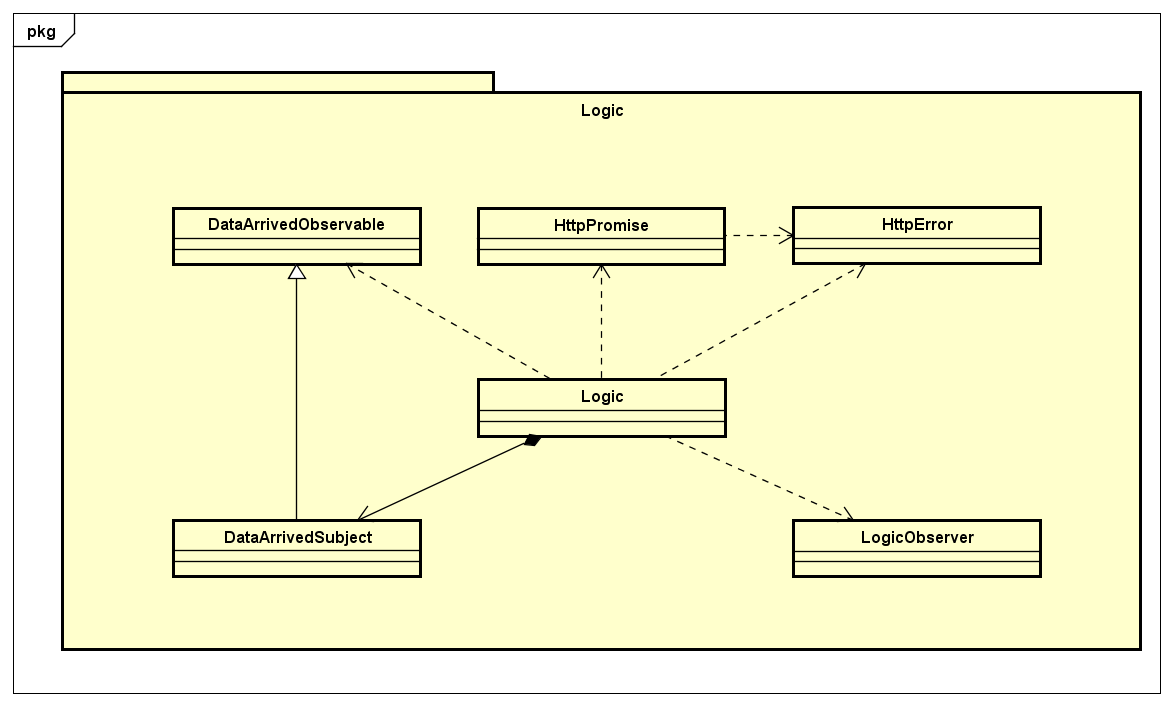
\includegraphics[width=\textwidth,height=\textheight,keepaspectratio]{images/diagrams/client/Client/Logic.png}
	\caption{Package Client::Logic}
\end{figure}
\newpage


\subsection{Client::Recorder}
Package contenente le componenti che realizzano il \gl{text to speech}. Vengono offerte funzionalità che permettono: \begin{itemize} \item la reazione a dei dati arrivati come riposta dal \file{Back-end}; \item la riproduzione audio del testo fornito come risposta dall'assistente virtuale. \end{itemize}
\begin{figure}[h] \centering 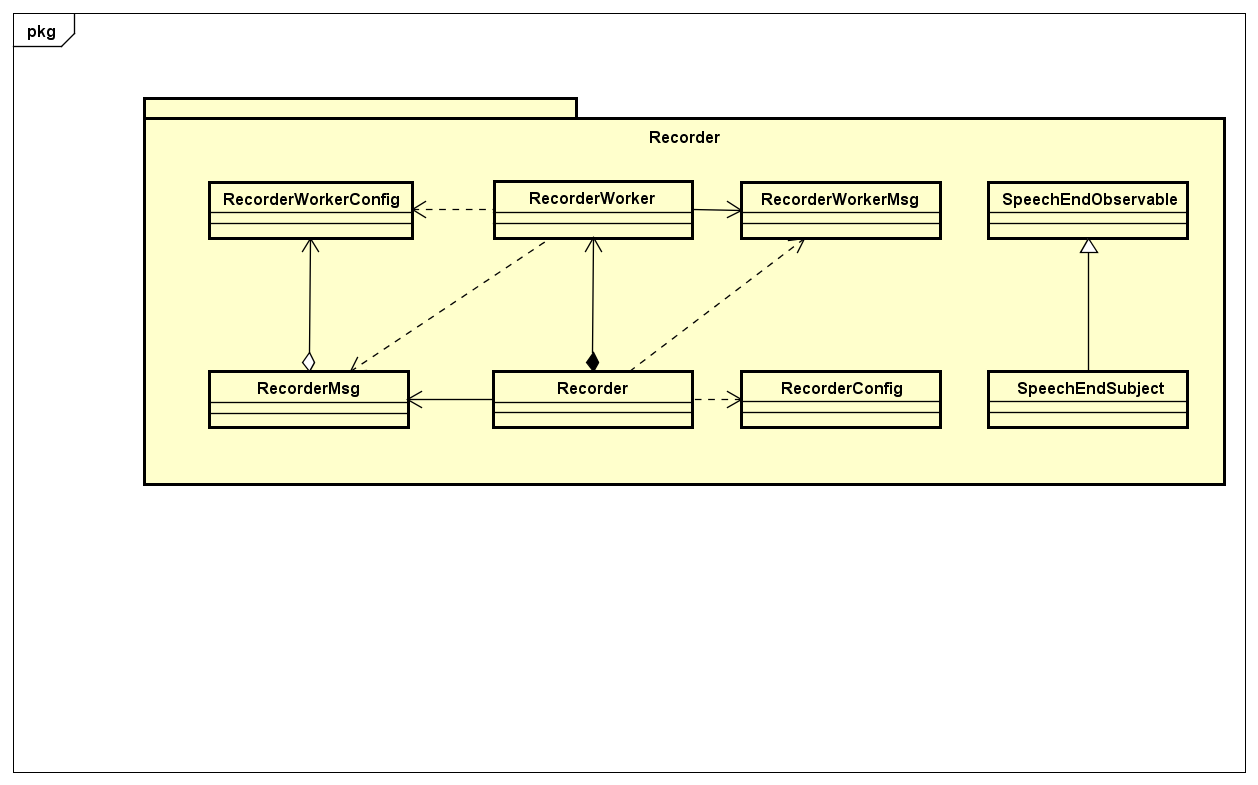
\includegraphics[width=\textwidth,height=\textheight,keepaspectratio]{images/diagrams/client/Client/Recorder.png}
	\caption{Package Client::Recorder}
\end{figure}
\newpage


\subsection{Client::TTS}
Package contenente le componenti che realizzano il text to speech. Vengono offerte funzionalità che permettono: \begin{itemize} \item la reazione a dei dati arrivati come riposta dal \file{Back-end}; \item la riproduzione audio del testo fornito come risposta dall'assistente virtuale. \end{itemize}
\begin{figure}[h] \centering 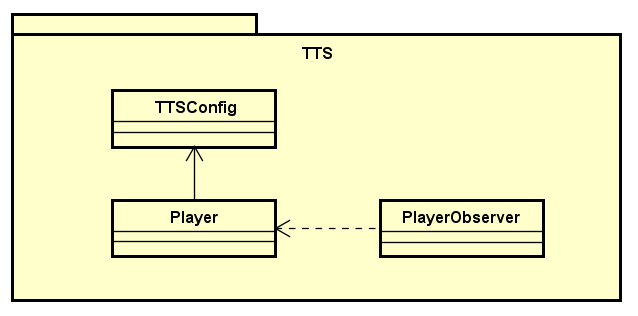
\includegraphics[width=\textwidth,height=\textheight,keepaspectratio]{images/diagrams/client/Client/TTS.png}
	\caption{Package Client::TTS}
\end{figure}
\newpage


\subsection{Client::Utility}
Package contenente classi e interfacce, dallo scopo generico, utili ad altri package del client.
\begin{figure}[h] \centering 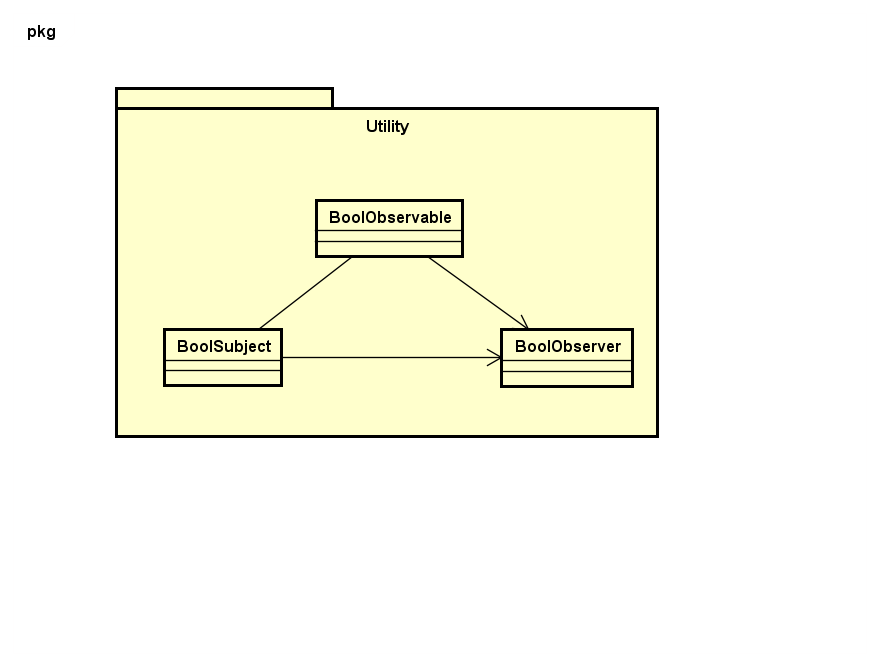
\includegraphics[width=\textwidth,height=\textheight,keepaspectratio]{images/diagrams/client/Client/Utility.png}
	\caption{Package Client::Utility}
\end{figure}
\newpage
\section{Specifica dei componenti}
\section{Diagrammi di sequenza}\label{sequenza}
In questa sezione vengono descritte e rappresentate tramite diagrammi di sequenza \gl{UML} le principali azioni lato back-end con lo scopo di facilitare la comprensione del funzionamento del \gl{sistema}. Per quest'ultimo motivo i diagrammi di sequenza non rappresentano l'effettiva realtà ma una sua approssimazione che non rifletterà appieno l'implementazione.\\
Le funzioni asincrone che ottengono i dati richiesti tramite callback sono rappresentati da una richiesta raffigurata da una freccia asincrona (freccia continua con punta aperta, notazione UML 2.5), e da una risposta chiamata \file{callback()} rappresentata anch'essa da una freccia asincrona, per indicare che la risposta sarà restituita una volta che la risorsa richiesta diverrà disponibile.

\subsection{Interazioni passate con la persona interagente}
Il diagramma qui riportato rappresenta la chiamata al \gl{webhook} da parte di api.ai per la ricerca di interazioni passate con la persona interagente . L'interazione inizia con la chiamata del metodo \file{webhook} fornito dalla classe \file{ConversationWebhookService} da parte di \file{api.ai}. Il metodo si occupa di ottenere la lista degli \file{User} con il metodo \file{getUserList} fornito dalla classe \file{UsersDAO}. Una volta ottenuta la lista degli \file{Users} viene controllato se la persona interagente è un amministratore. Se lo è il \file{context} della \file{lambda function} viene settato ad \file{admin}, in modo che api.ai riconosca l'utente come un potenziale amministratore e gli chieda se vuole entrare nell'area di amministrazione. Se non è un amministratore viene richiesta la lista dei \file{Guest} attraverso il metodo \file{getGuestList} fornito dalla classe \file{GuestsDAO}. Una volta ottenuta la lista viene controllato se la persona interagente è un ospite con cui si ha già avuto una o più interazioni passate. Se ciò è avvenuto il \file{context accoglienza} viene riempito con l'azienda e i dati della persona con cui l'ospite ha avuto il maggior numero di incontri in passato, e viene chiesto di confermare se la persona indicata è quella a cui l'ospite è effettivamente interessato. Se il suo nome invece non viene trovato nella lista dei \file{Guests}, la persona interagente verrà trattata come un nuovo ospite.
\begin{figure}[h] \centering 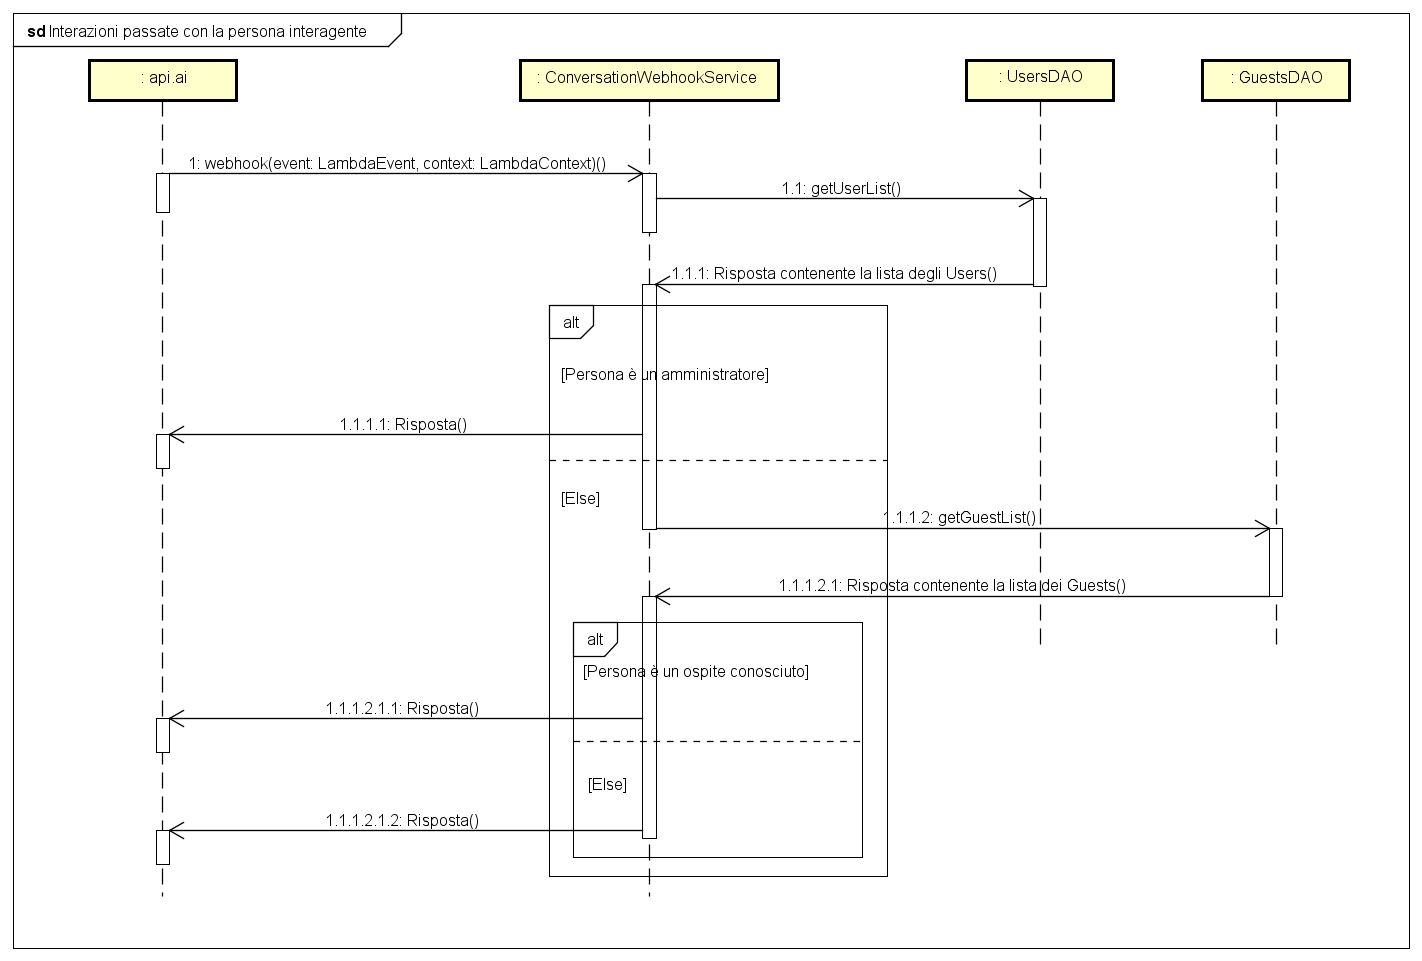
\includegraphics[width=\textwidth,height=\textheight,keepaspectratio]{images/diagrams/back-end/Ufficial_Backend/Interazionipassateconlapersonainteragente.png}
\caption{Interazioni passate con la persona interagente}
\end{figure}
\newpage
\subsection{Interazione tra service e client}
Il diagramma qui riportato rappresenta l'interazione tra service e client per mezzo della chiamata al metodo \file{queryLambda} fornito dalla classe \file{VocalAPI}, il quale permette di dedurre il servizio necessario al client vocale e successivamente offrire il servizio qualora il service ne sia in grado. Per il riconoscimento dell'azione viene invocato il metodo \file{speechToText} della classe \file{STTModule}, che ritorna l'azione necessaria al client vocale a partire da un file audio. Una volta ottenuta l'azione viene controllato il valore del campo \file{action} di tale risposta. Nel caso in cui \file{action} non corrisponda ad una delle azioni supportate, ovvero action è un'azione che non richiede operazione da parte del back-end oppure \file{actionIncomplete} è impostato a true, tale risposta viene rielaborata ed inoltrata al client. Se invece l'action è supportata, il metodo si occupa di eseguire le azioni necessarie utilizzando i metodi privati della classe \file{VocalAPI}. In quest'ultimo caso viene inoltre pubblicato un messaggio su un topic di \file{SNS}, utilizzando il metodo \file{publish}, in modo che sia possibile registrare i dati relativi a tali interazioni e mandare le notifiche ai membri interessati.
 \begin{figure}[h]
  \centering
  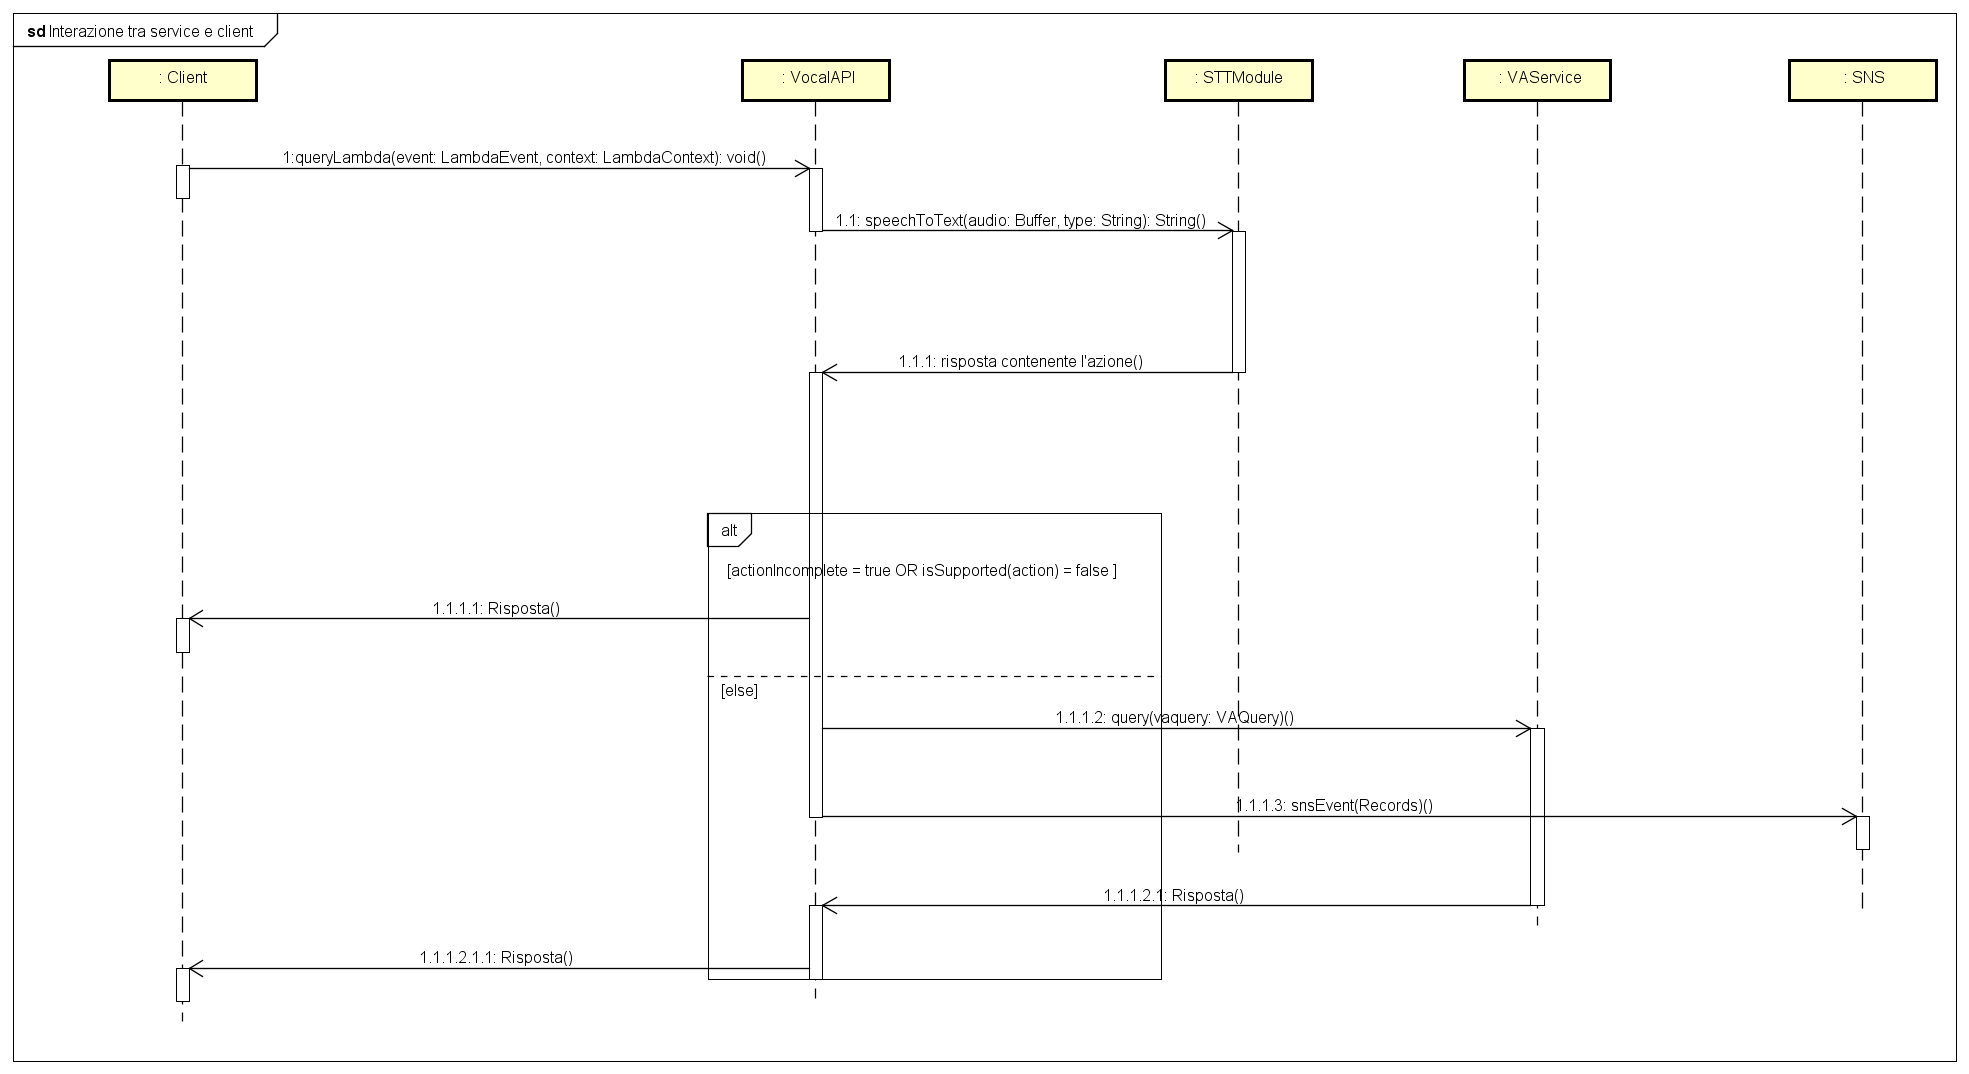
\includegraphics[width=\textwidth,height=\textheight,keepaspectratio]{images/diagrams/back-end/Ufficial_Backend/Interazionetraserviceeclient.png}
 \caption{Interazione tra service e client}
\end{figure}
\newpage
\hypertarget{interazioneVocalAPIVAService}{\subsection{Interazione tra VocalAPI e VAService}}
Il diagramma qui riportato rappresenta l'interrogazione dell'assistente virtuale per mezzo della chiamata alla Lambda Function \file{query} fornita dalla classe \file{VAService}. Inizialmente viene invocato il metodo \file{getAgent} fornito dalla classe \file{AgentsDAO} per ottenere, a partire dal nome dell'applicazione contenuto nella richiesta, il token identificativo dell'Agent che si vuole interrogare. Una volta ottenuto il token viene eseguita una chiamata all'endpoint \file{/query} di api.ai per mezzo della classe \file{VAModule} utilizzando il testo presente nella richiesta. Infine, a partire dalla risposta ricevuta da tale serivizo, viene inviata la risposta a VocalAPI utilizzando il context della Lambda Function.
 \begin{figure}[h]
  \centering
  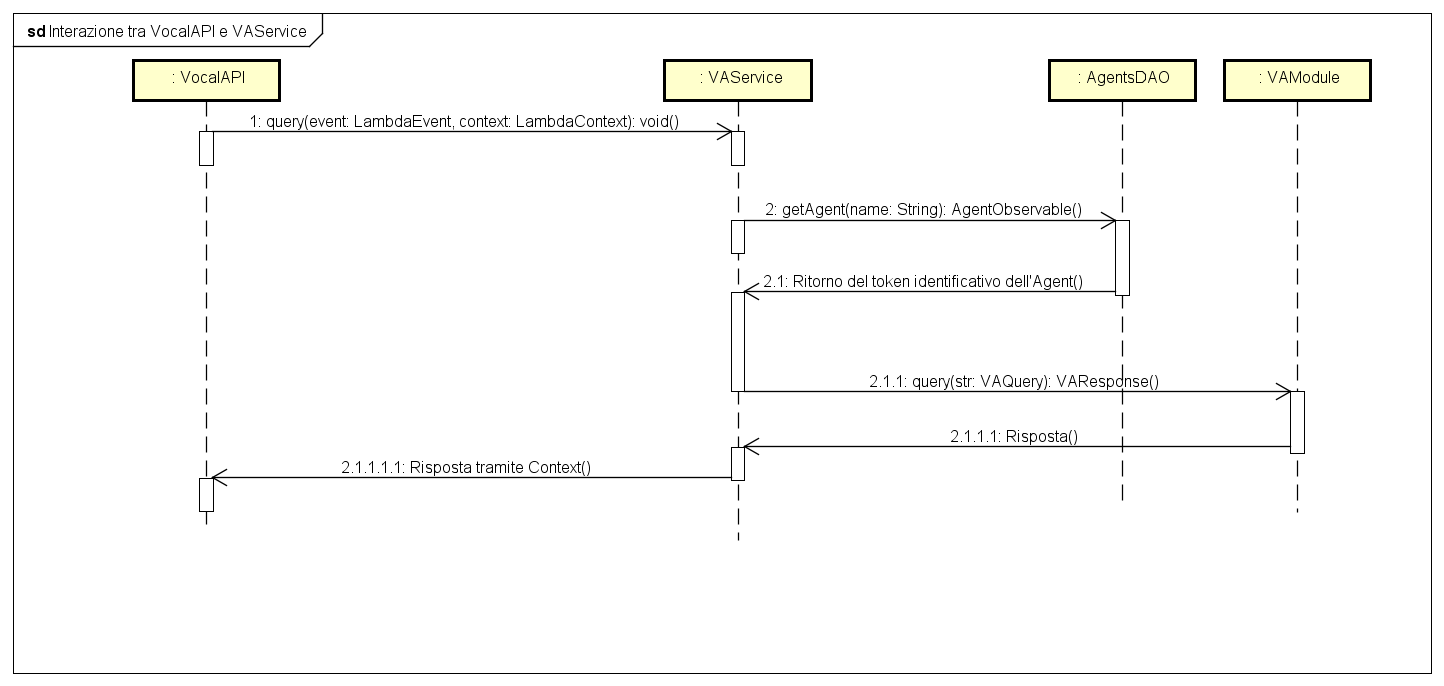
\includegraphics[width=\textwidth,height=\textheight,keepaspectratio]{images/diagrams/back-end/Ufficial_Backend/Interazione tra VocalAPI e VAService.png}
 \caption{Interazione tra VocalAPI e VAService.png}
\end{figure}
\newpage

\subsection{Verifica autenticazione}
Il diagramma qui riportato rappresenta la \gl{verifica} di un'autenticazione ad ogni interazione dell'agent di amministrazione per via del webhook fornito dalla classe \file{AdministrationWebhookService}. Tale metodo si occupa di verificare che nella richiesta sia presente un \gl{JSON} Web Token (\file{JWT}) che confermi un'autenticazione avvenuta con successo. In caso di mancata autenticazione, il campo \file{status} della risposta sarà impostato a 403. Nel caso in cui il token sia presente e valido, ovvero che la firma sia valida ed il token non sia scaduto, tale campo sarà invece impostato a 200, ed il campo \file{speech} della risposta sarà copiato da \file{fulfillment.speech} della richiesta, risultando quindi in una risposta uguale a quella definita nell'agente di api.ai.
 \begin{figure}[h] \centering 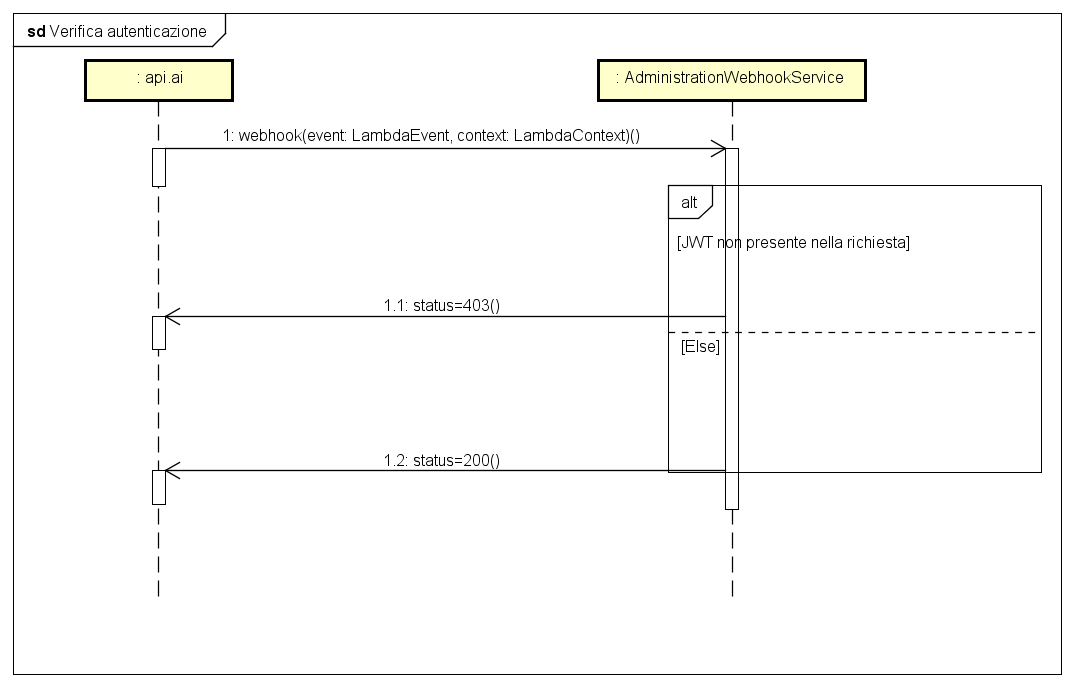
\includegraphics[width=\textwidth,height=\textheight,keepaspectratio]{images/diagrams/back-end/Ufficial_Backend/Verificaautenticazione.png} 	\caption{Verifica autenticazione}
\end{figure}
\newpage


\subsection{Back-end::Users::UsersService::addUser}
Il diagramma qui riportato rappresenta l'implementazione della lambda function che si occupa di aggiungere un \file{User} al sistema attraverso il metodo \file{addUser}.
 \begin{figure}[h] \centering 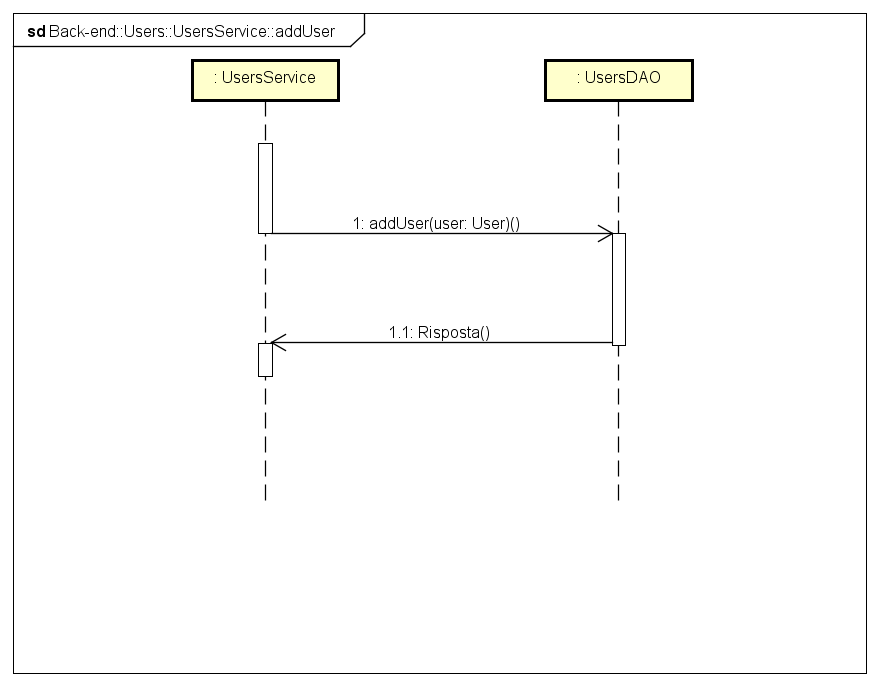
\includegraphics[width=\textwidth,height=\textheight,keepaspectratio]{images/diagrams/back-end/Ufficial_Backend/Back-endUsersUsersServiceaddUser.png} 	\caption{Back-end::Users::UsersService::addUser}
\end{figure}

\newpage
\subsection{Back-end::Users::UsersService::getUser}
Il diagramma qui riportato rappresenta l'implementazione della lambda function che si occupa di ottenere un \file{User} del sistema attraverso il metodo \file{getUser}.  \begin{figure}[h] \centering 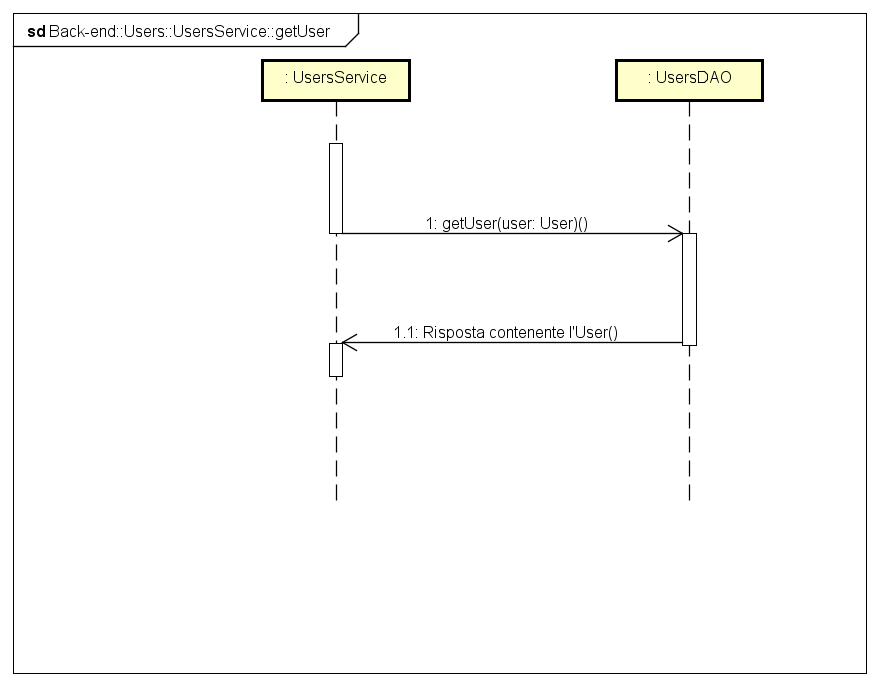
\includegraphics[width=\textwidth,height=\textheight,keepaspectratio]{images/diagrams/back-end/Ufficial_Backend/Back-endUsersUsersServicegetUser.png} 	\caption{Back-end::Users::UsersService::getUser}
\end{figure}
\newpage

\subsection{Back-end::Users::UsersService::getUserList}
Il diagramma qui riportato rappresenta l'implementazione della lambda function che si occupa di ottenere la lista degli \file{User} del sistema attraverso il metodo \file{getUserList}.
\begin{figure}[h] \centering 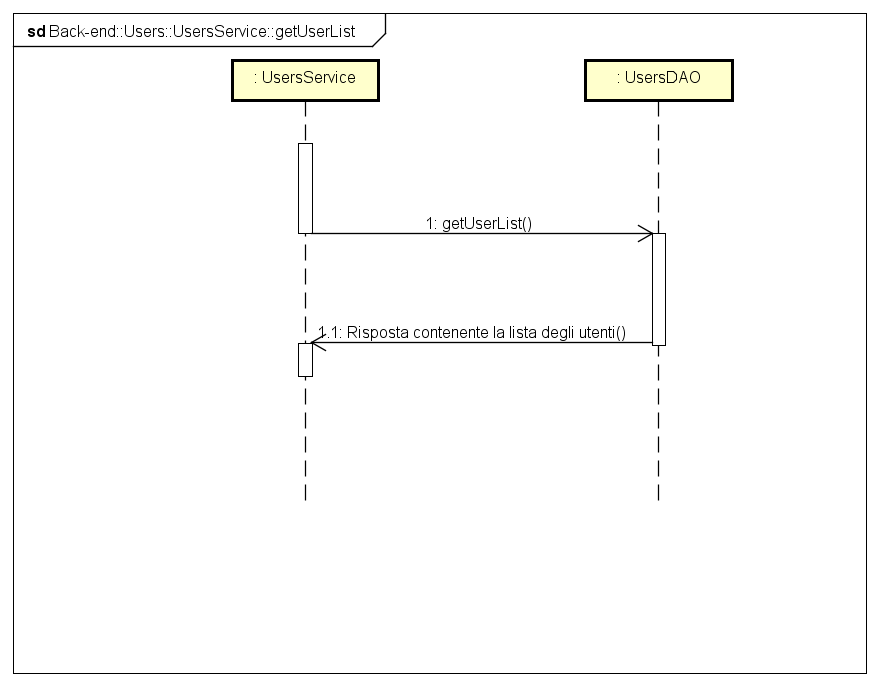
\includegraphics[width=\textwidth,height=\textheight,keepaspectratio]{images/diagrams/back-end/Ufficial_Backend/Back-endUsersUsersServicegetUserList.png} 	\caption{Back-end::Users::UsersService::getUserList}
\end{figure}
\newpage

\subsection{Back-end::Users::UsersService::deleteUser}
Il diagramma qui riportato rappresenta l'implementazione della lambda function che si occupa di rimuovere un \file{User} dal sistema attraverso il metodo \file{removeUser}.
\begin{figure}[h] \centering 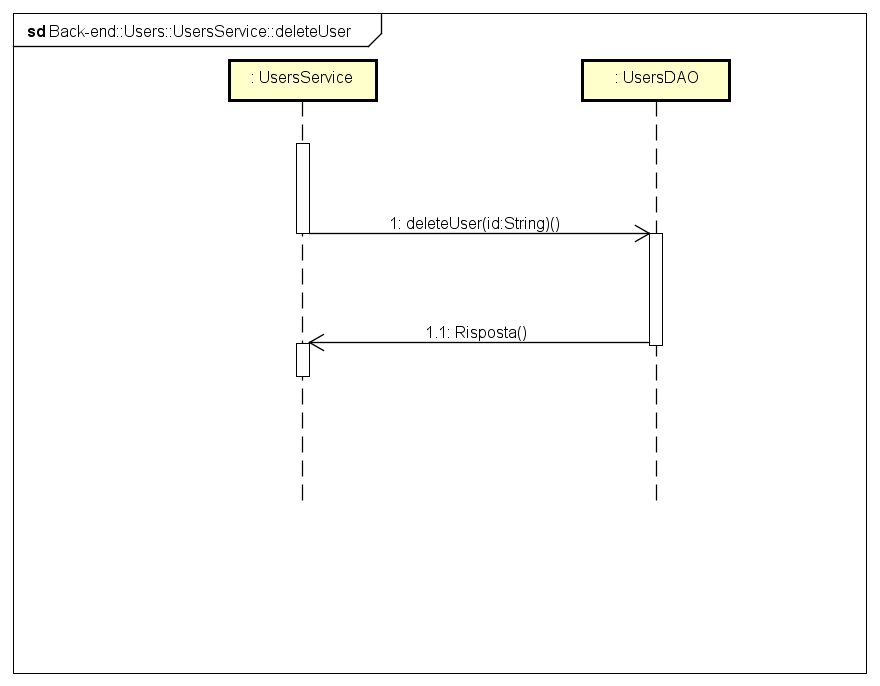
\includegraphics[width=\textwidth,height=\textheight,keepaspectratio]{images/diagrams/back-end/Ufficial_Backend/Back-endUsersUsersServicedeleteUser.png} 	\caption{Back-end::Users::UsersService::deleteUser}
\end{figure}
\newpage

\subsection{Back-end::Users::UsersService::updateUser}
Il diagramma qui riportato rappresenta l'implementazione della lambda function che si occupa di modificare un \file{User} del sistema attraverso il metodo \file{updateUser}.
\begin{figure}[h] \centering 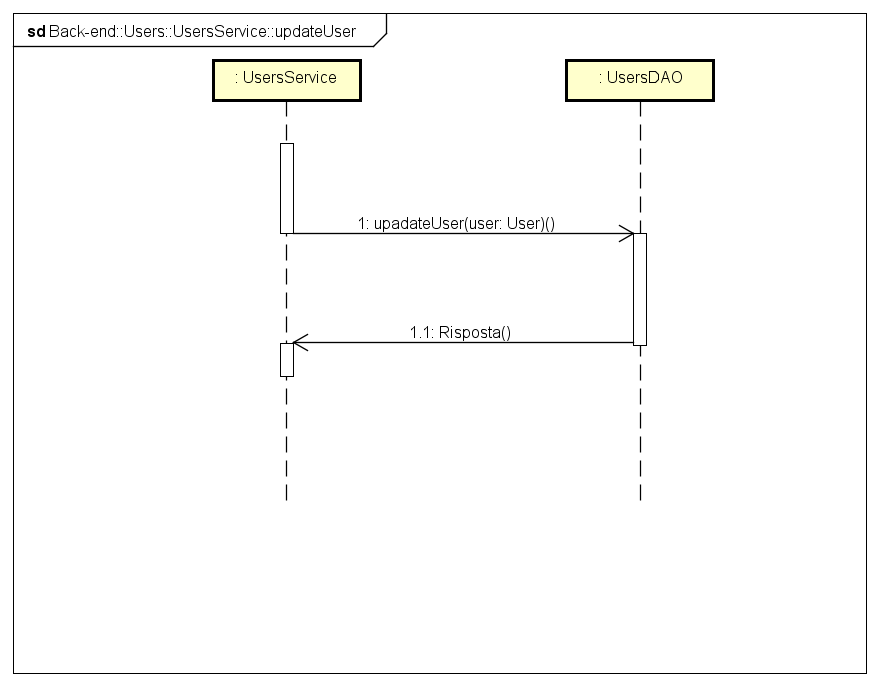
\includegraphics[width=\textwidth,height=\textheight,keepaspectratio]{images/diagrams/back-end/Ufficial_Backend/Back-endUsersUsersServiceupdateUser.png} 	\caption{Back-end::Users::UsersService::updateUser}
\end{figure}
\newpage

\subsection{Back-end::Users::UsersDAODynamoDBaddUser}
Il diagramma qui riportato rappresenta l'aggiunta di un \file{User} al database attraverso il metodo \file{put} del \file{DocumentClient} di \file{DynamoDB}, utilizzando la risposta come parametro per chiamare la funzione di \gl{callback}.
\begin{figure}[h] \centering 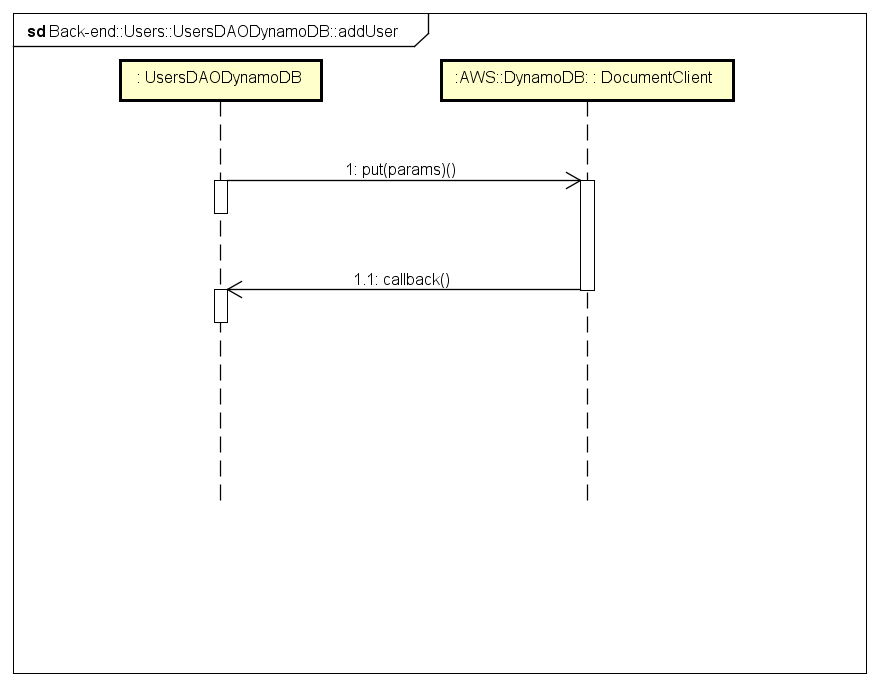
\includegraphics[width=\textwidth,height=\textheight,keepaspectratio]{images/diagrams/back-end/Ufficial_Backend/Back-endUsersUsersDAODynamoDBaddUser.png} 	\caption{Back-end::Users::UsersDAODynamoDBaddUser}
\end{figure}
\newpage
\subsection{Back-end::Users::UsersDAODynamoDBgetUser}
Il diagramma qui riportato rappresenta l'ottenimento di un \file{User} dal database attraverso il metodo \file{get} del \file{DocumentClient} di \file{DynamoDB}, utilizzando la risposta come parametro per chiamare la funzione di callback.
\begin{figure}[h] \centering 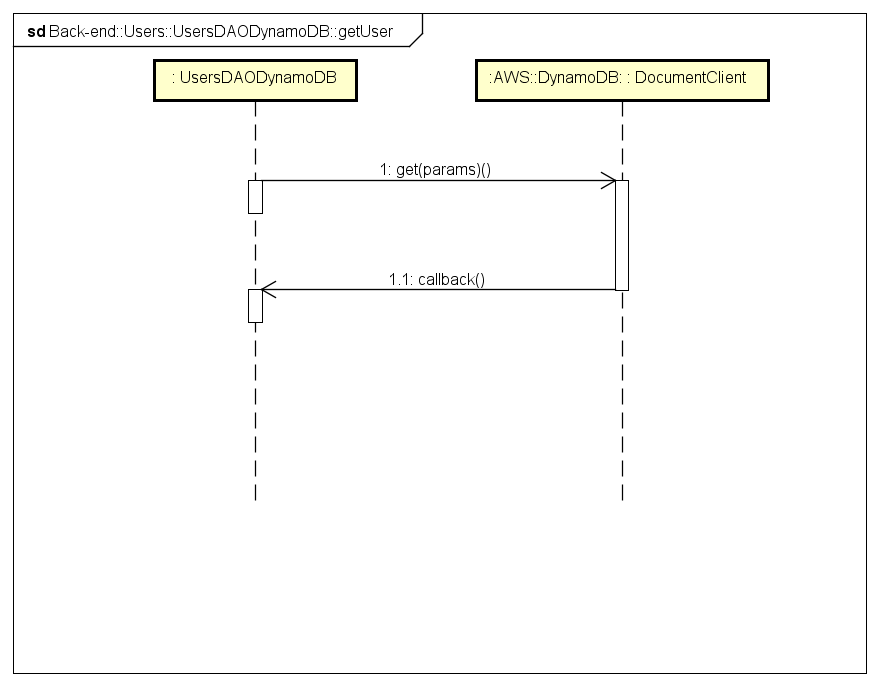
\includegraphics[width=\textwidth,height=\textheight,keepaspectratio]{images/diagrams/back-end/Ufficial_Backend/Back-endUsersUsersDAODynamoDBgetUser.png} 	\caption{Back-end::Users::UsersDAODynamoDBgetUser}
\end{figure}
\newpage
\subsection{Back-end::Users::UsersDAODynamoDBgetUserList}
Il diagramma qui riportato rappresenta l'ottenimento della lista di \file{User} dal database attraverso il metodo \file{scan} del \file{DocumentClient} di \file{DynamoDB}, utilizzando la risposta come parametro per chiamare la funzione di callback. Poichè il metodo \file{scan} del \file{DocumentClient} permette al più il ritorno di una lista delle dimensioni di 1MB, se il campo LastEvaluetedKey è settato allora non tutti gli \file{User} sono stati ritornati, e quindi è necessario rieseguire il metodo scan fornendo come parametro d'ingresso la chiave da cui ripartire per l'estrazione dei dati. Se invece tale campo non è settato allora è stata ritornata l'intera lista.
\begin{figure}[h] \centering 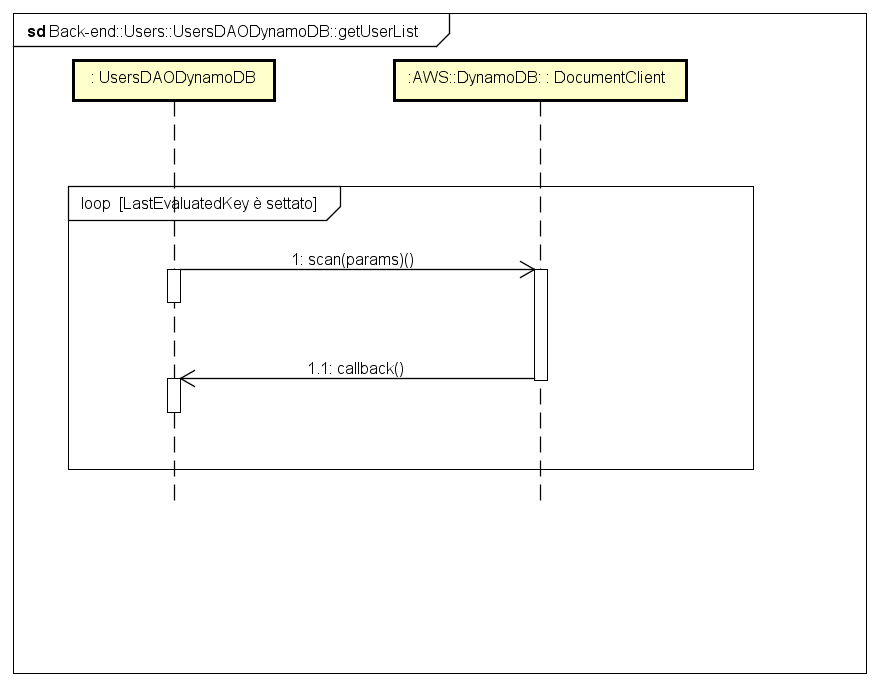
\includegraphics[width=\textwidth,height=\textheight,keepaspectratio]{images/diagrams/back-end/Ufficial_Backend/Back-endUsersUsersDAODynamoDBgetUserList.png} 	\caption{Back-end::Users::UsersDAODynamoDBgetUserList}
\end{figure}
\newpage

\subsection{Back-end::Users::UsersDAODynamoDB::removeUser}
Il diagramma qui riportato rappresenta la rimozione di un \file{User} dal database attraverso il metodo \file{delete} del \file{DocumentClient} di \file{DynamoDB}, utilizzando la risposta come parametro per chiamare la funzione di callback.
 \begin{figure}[h] \centering 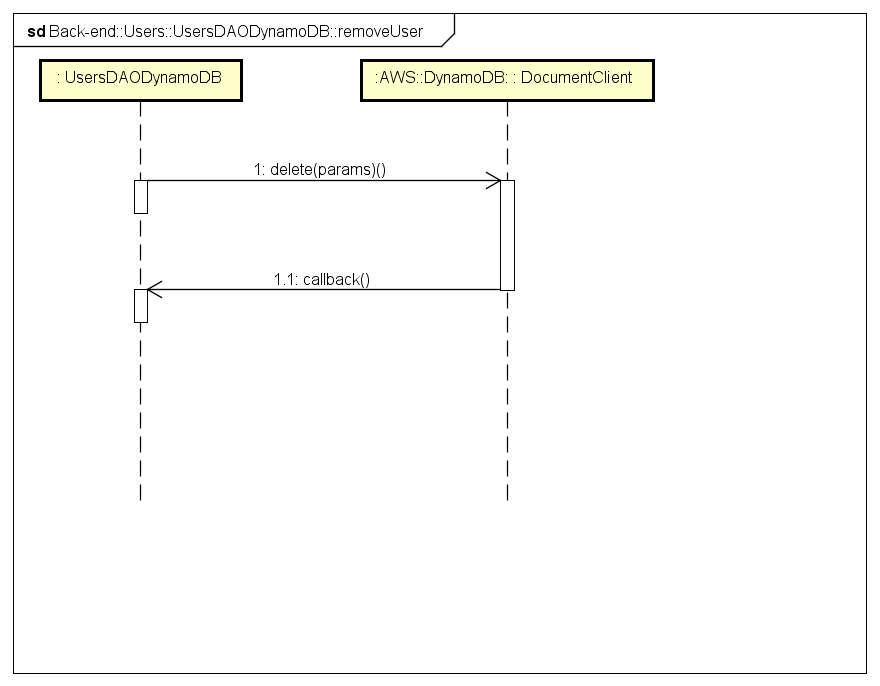
\includegraphics[width=\textwidth,height=\textheight,keepaspectratio]{images/diagrams/back-end/Ufficial_Backend/Back-endUsersUsersDAODynamoDBremoveUser.png} 	\caption{Back-end::Users::UsersDAODynamoDB::removeUser}
\end{figure}
\newpage

\subsection{Back-end::Users::UsersDAODynamoDB::updateUser}
Il diagramma qui riportato rappresenta la modifica di un \file{User} del database attraverso il metodo \file{update} del \file{DocumentClient} di \file{DynamoDB}, utilizzando la risposta come parametro per chiamare la funzione di callback.
\begin{figure}[h] \centering 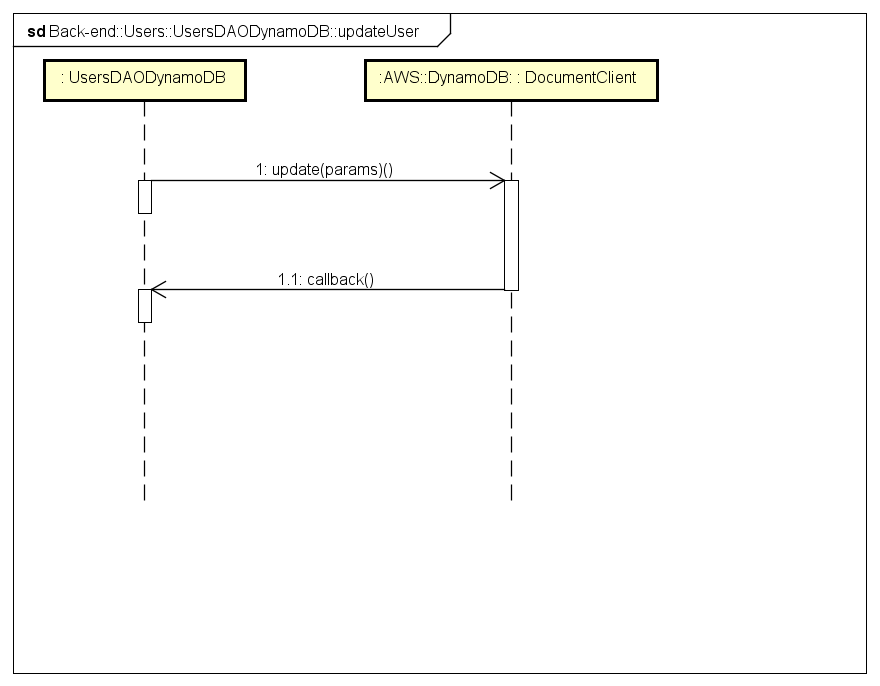
\includegraphics[width=\textwidth,height=\textheight,keepaspectratio]{images/diagrams/back-end/Ufficial_Backend/Back-endUsersUsersDAODynamoDBupdateUser.png} 	\caption{Back-end::Users::UsersDAODynamoDB::updateUser}
\end{figure}
\newpage


\subsection{Back-end::ConversationsDAODynamoDB::addConversation}
Il diagramma qui riportato rappresenta l'aggiunta di una \file{Conversation} al database attraverso il metodo \file{put} del \file{DocumentClient} di \file{DynamoDB}, utilizzando la risposta come parametro per chiamare la funzione di callback.
 \begin{figure}[h] \centering 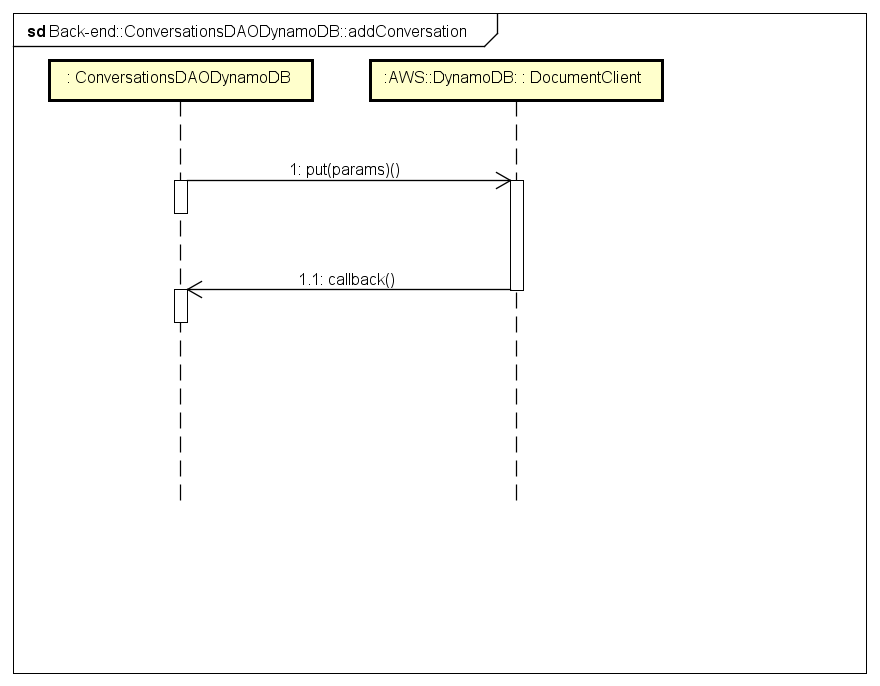
\includegraphics[width=\textwidth,height=\textheight,keepaspectratio]{images/diagrams/back-end/Ufficial_Backend/Back-endConversationsDAODynamoDBaddConversation.png} 	\caption{Back-end::ConversationsDAODynamoDB::addConversation}
\end{figure}
\newpage

\subsection{Back-end::ConversationsDAODynamoDB::addMessage}
Il diagramma qui riportato rappresenta l'aggiunta di un \file{Message} al database attraverso il metodo \file{put} del \file{DocumentClient} di \file{DynamoDB}, utilizzando la risposta come parametro per chiamare la funzione di callback.
 \begin{figure}[h] \centering 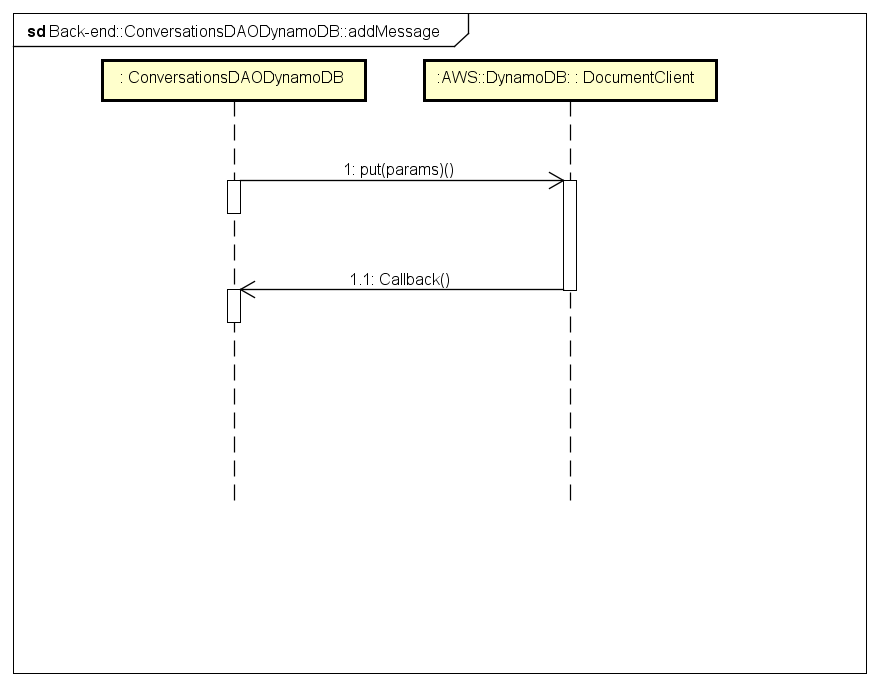
\includegraphics[width=\textwidth,height=\textheight,keepaspectratio]{images/diagrams/back-end/Ufficial_Backend/Back-endConversationsDAODynamoDBaddMessage.png} 	\caption{Back-end::ConversationsDAODynamoDB::addMessage}
\end{figure}
\newpage

\subsection{Back-end::ConversationsDAODynamoDB::getConversation}
Il diagramma qui riportato rappresenta l'ottenimento di una \file{Conversation} dal database attraverso il metodo \file{get} del \file{DocumentClient} di \file{DynamoDB}, utilizzando la risposta come parametro per chiamare la funzione di callback.
 \begin{figure}[h] \centering 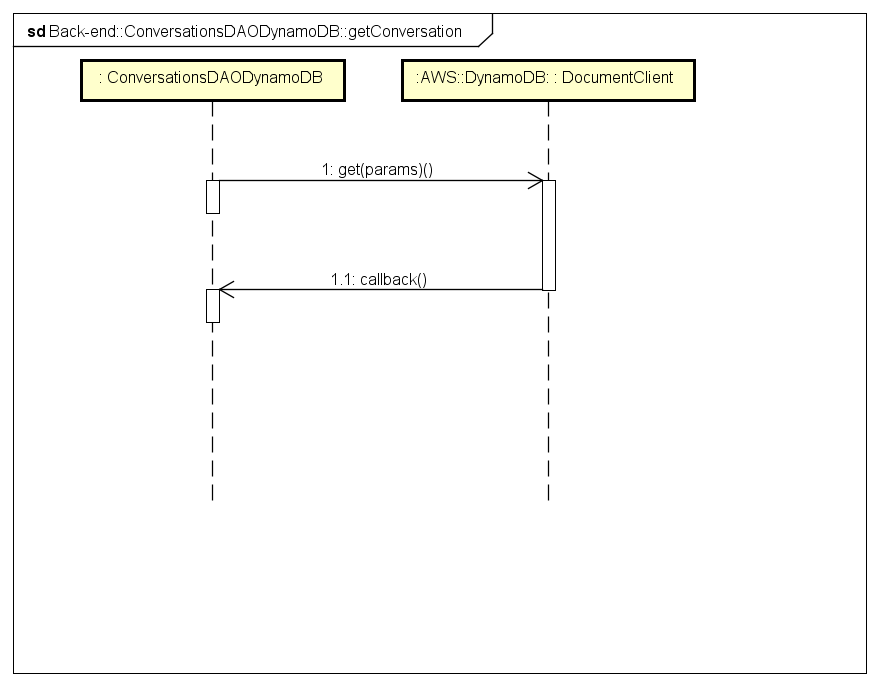
\includegraphics[width=\textwidth,height=\textheight,keepaspectratio]{images/diagrams/back-end/Ufficial_Backend/Back-endConversationsDAODynamoDBgetConversation.png} 	\caption{Back-end::ConversationsDAODynamoDB::getConversation}
\end{figure}
\newpage

\subsection{Back-end::ConversationsDAODynamoDB::getConversationList}
Il diagramma qui riportato rappresenta l'ottenimento della lista di \file{Conversation} dal database attraverso il metodo \file{scan} del \file{DocumentClient} di \file{DynamoDB}, utilizzando la risposta come parametro per chiamare la funzione di callback. Poichè il metodo \file{scan} del \file{DocumentClient} permette al più il ritorno di una lista delle dimensioni di 1MB, se il campo LastEvaluetedKey è settato allora non tutti le \file{Conversation} sono state ritornate, e quindi è necessario rieseguire il metodo scan fornendo come parametro d'ingresso la chiave da cui ripartire per l'estrazione dei dati. Se invece tale campo non è settato allora è stata ritornata l'intera lista.
 \begin{figure}[h] \centering 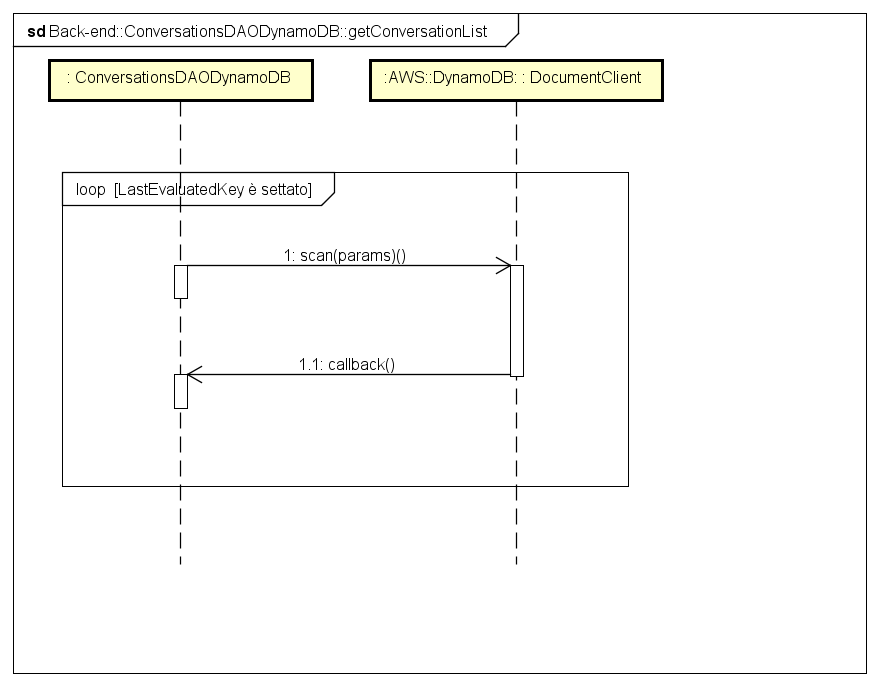
\includegraphics[width=\textwidth,height=\textheight,keepaspectratio]{images/diagrams/back-end/Ufficial_Backend/Back-endConversationsDAODynamoDBgetConversationList.png} 	\caption{Back-end::ConversationsDAODynamoDB::getConversationList}
\end{figure}
\newpage

\subsection{Back-end::ConversationsDAODynamoDB::removeConversation}
Il diagramma qui riportato rappresenta la rimozione di una \file{Conversation} dal database attraverso il metodo \file{delete} del \file{DocumentClient} di \file{DynamoDB}, utilizzando la risposta come parametro per chiamare la funzione di callback.
\begin{figure}[h] \centering 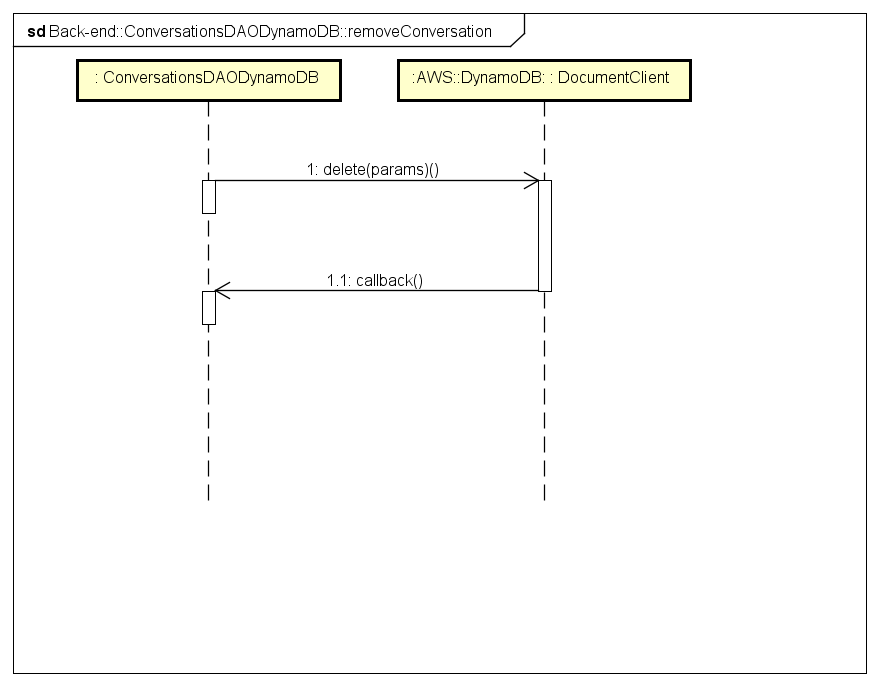
\includegraphics[width=\textwidth,height=\textheight,keepaspectratio]{images/diagrams/back-end/Ufficial_Backend/Back-endConversationsDAODynamoDBremoveConversation.png} 	\caption{Back-end::ConversationsDAODynamoDB::removeConversation}
\end{figure}

\newpage

\subsection{Back-end::GuestsDAODynamoDB::addGuest}
Il diagramma qui riportato rappresenta l'aggiunta di un \file{Guest} al database attraverso il metodo \file{add} del \file{DocumentClient} di \file{DynamoDB}, utilizzando la risposta come parametro per chiamare la funzione di callback.
\begin{figure}[h] \centering 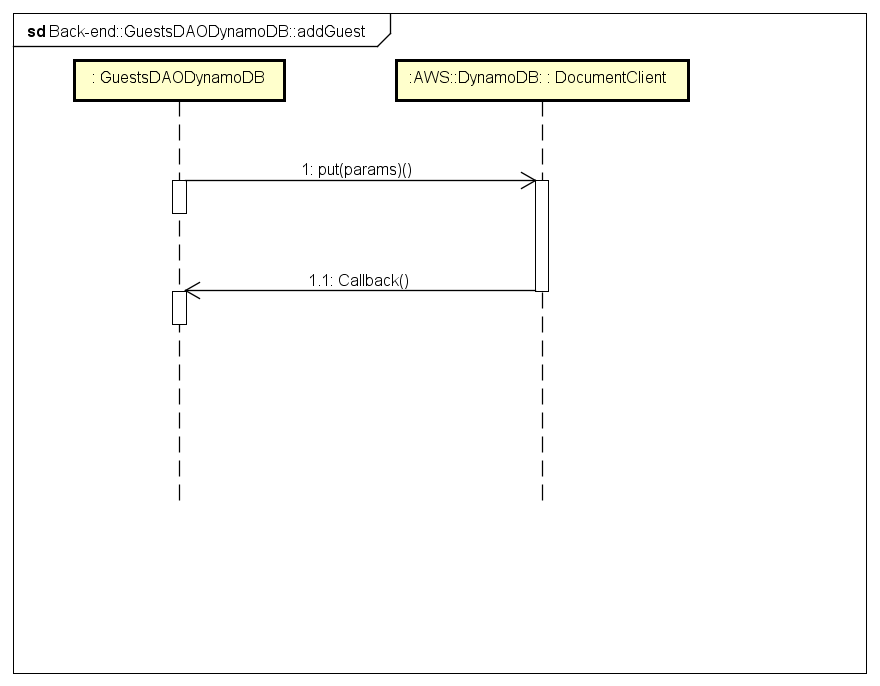
\includegraphics[width=\textwidth,height=\textheight,keepaspectratio]{images/diagrams/back-end/Ufficial_Backend/Back-endGuestsDAODynamoDBaddGuest.png} 	\caption{Back-end::GuestsDAODynamoDB::addGuest}
\end{figure}
\newpage

\subsection{Back-end::ConversationsDAODynamoDB::getGuest}
Il diagramma qui riportato rappresenta l'ottenimento di un \file{Guest} dal database attraverso il metodo \file{get} del \file{DocumentClient} di \file{DynamoDB}, utilizzando la risposta come parametro per chiamare la funzione di callback.
 \begin{figure}[h] \centering 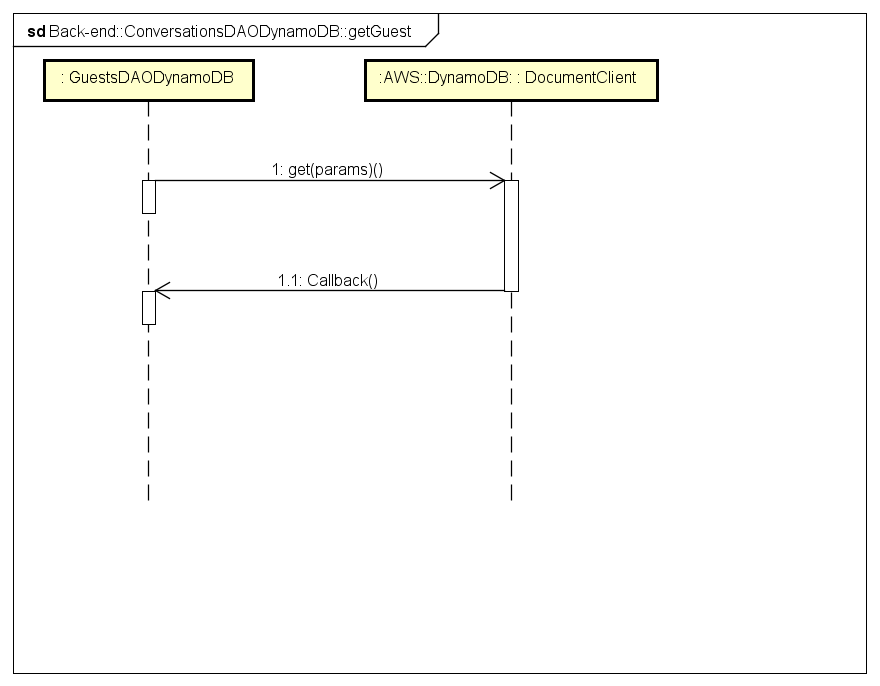
\includegraphics[width=\textwidth,height=\textheight,keepaspectratio]{images/diagrams/back-end/Ufficial_Backend/Back-endConversationsDAODynamoDBgetGuest.png} 	\caption{Back-end::ConversationsDAODynamoDB::getGuest}
\end{figure}
\newpage

\subsection{Back-end::ConversationsDAODynamoDB::getGuestList}
Il diagramma qui riportato rappresenta l'ottenimento della lista di \file{Guest} dal database attraverso il metodo \file{scan} del \file{DocumentClient} di \file{DynamoDB}, utilizzando la risposta come parametro per chiamare la funzione di callback. Poichè il metodo \file{scan} del \file{DocumentClient} permette al più il ritorno di una lista delle dimensioni di 1MB, se il campo LastEvaluetedKey è settato allora non tutti i \file{Guest} sono stati ritornati, e quindi è necessario rieseguire il metodo scan fornendo come parametro d'ingresso la chiave da cui ripartire per l'estrazione dei dati. Se invece tale campo non è settato allora è stata ritornata l'intera lista.
 \begin{figure}[h] \centering 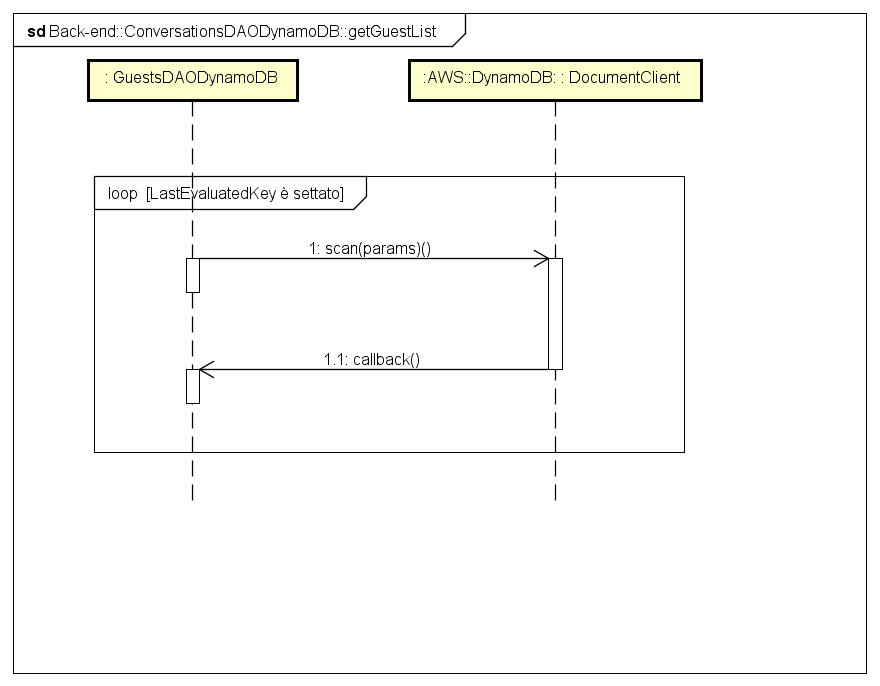
\includegraphics[width=\textwidth,height=\textheight,keepaspectratio]{images/diagrams/back-end/Ufficial_Backend/Back-endConversationsDAODynamoDBgetGuestList.png} 	\caption{Back-end::ConversationsDAODynamoDB::getGuestList}
\end{figure}

\newpage



\subsection{Back-end::ConversationsDAODynamoDB::removeGuest}
Il diagramma qui riportato rappresenta la rimozione di un \file{Guest} dal database attraverso il metodo \file{delete} del \file{DocumentClient} di \file{DynamoDB}, utilizzando la risposta come parametro per chiamare la funzione di callback.
 \begin{figure}[h] \centering 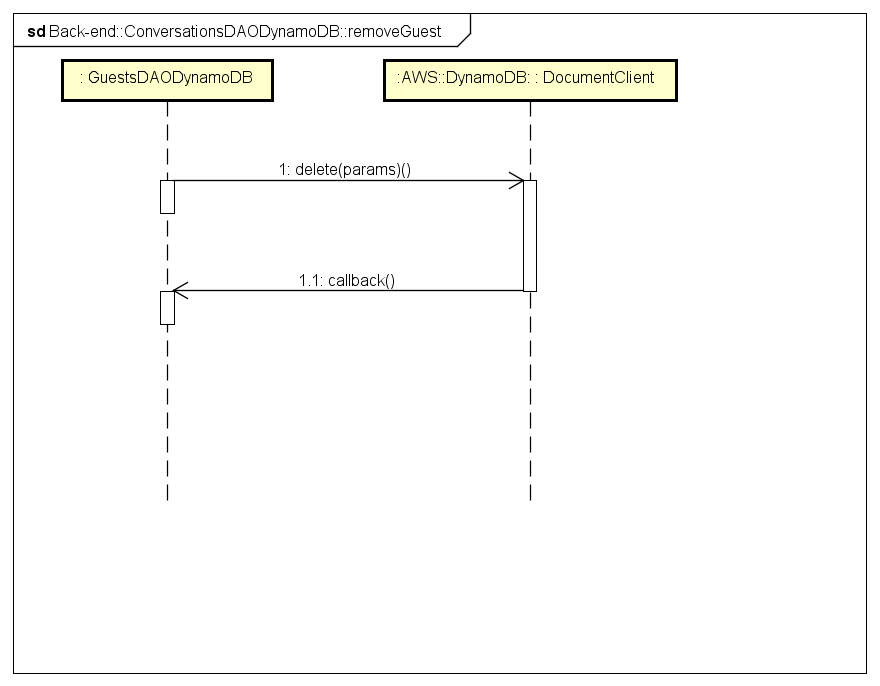
\includegraphics[width=\textwidth,height=\textheight,keepaspectratio]{images/diagrams/back-end/Ufficial_Backend/Back-endConversationsDAODynamoDBremoveGuest.png} 	\caption{Back-end::ConversationsDAODynamoDB::removeGuest}
\end{figure}

\newpage

\subsection{Back-end::ConversationsDAODynamoDB::updateGuest}
Il diagramma qui riportato rappresenta la modifica di un \file{Guest} del database attraverso il metodo \file{update} del \file{DocumentClient} di \file{DynamoDB}, utilizzando la risposta come parametro per chiamare la funzione di callback.
 \begin{figure}[h] \centering 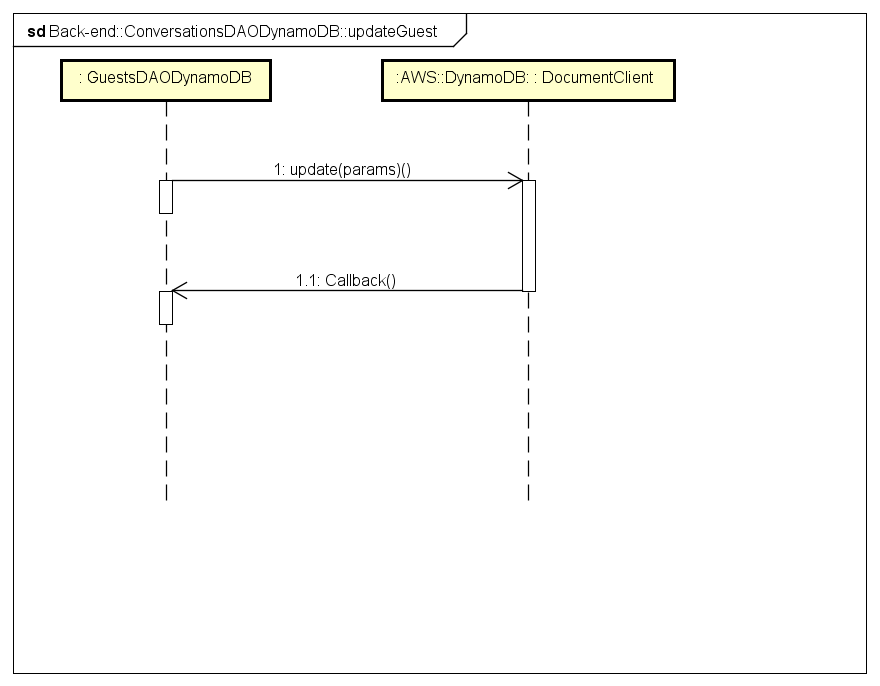
\includegraphics[width=\textwidth,height=\textheight,keepaspectratio]{images/diagrams/back-end/Ufficial_Backend/Back-endConversationsDAODynamoDBupdateGuest.png} 	\caption{Back-end::ConversationsDAODynamoDB::updateGuest}
\end{figure}
\newpage


\subsection{Back-end::Notifications::NotificationService::getChannelList}
Il diagramma qui riportato rappresenta la richiesta dei canali disponibili al servizio esterno \file{\gl{Slack}}, utilizzando il metodo \file{channels.list} messo a disposizione da \file{Slack}.
 \begin{figure}[h] \centering 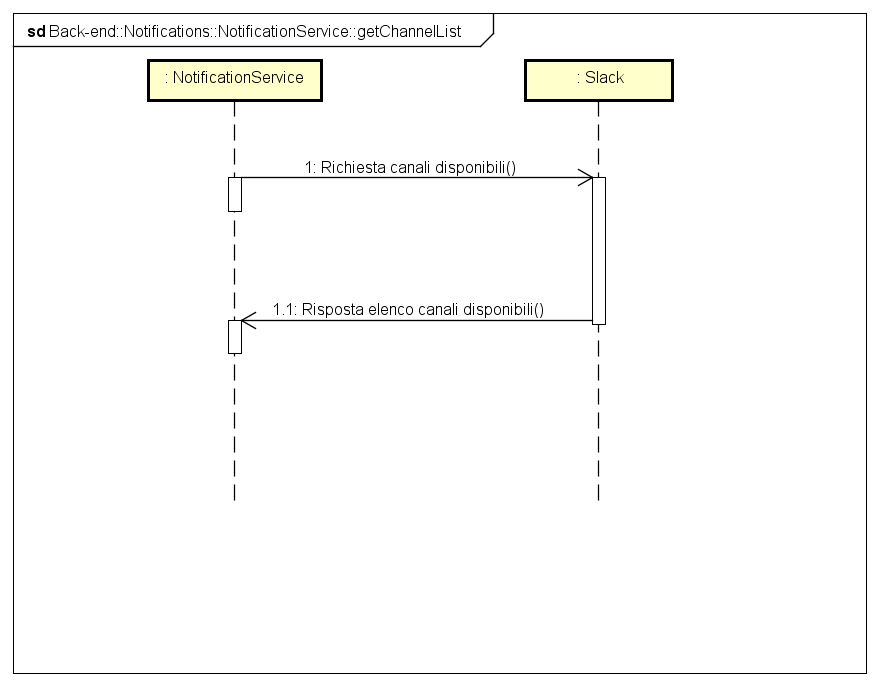
\includegraphics[width=\textwidth,height=\textheight,keepaspectratio]{images/diagrams/back-end/Ufficial_Backend/Back-endNotificationsNotificationServicegetChannelList.png} 	\caption{Back-end::Notifications::NotificationService::getChannelList}
\end{figure}
\newpage

\subsection{Back-end::Notifications::NotificationService::sendMsg}
Il diagramma qui riportato rappresenta l'invio di un messaggio al servizio esterno \file{Slack}.
 \begin{figure}[h] \centering 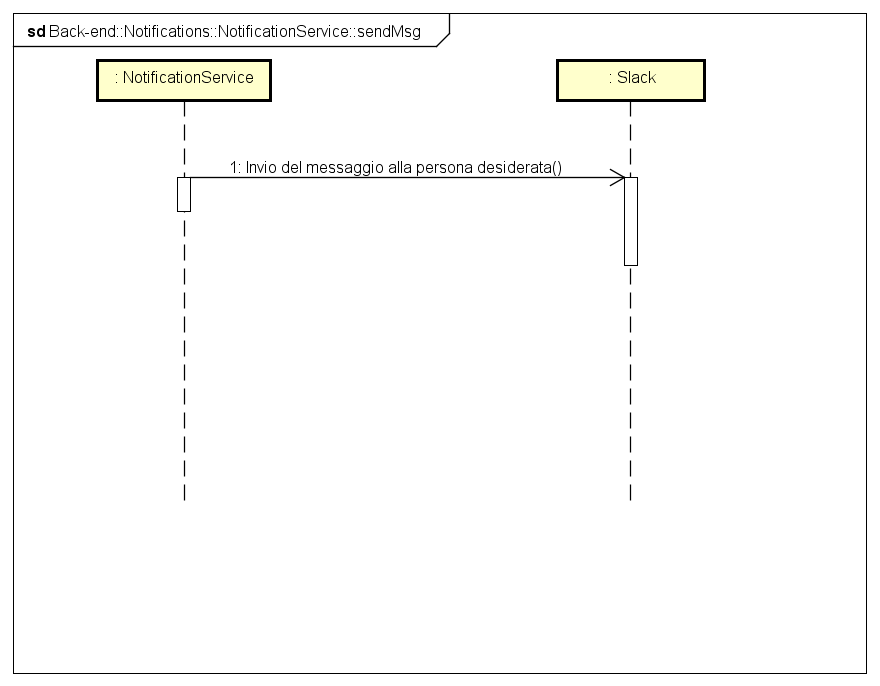
\includegraphics[width=\textwidth,height=\textheight,keepaspectratio]{images/diagrams/back-end/Ufficial_Backend/Back-endNotificationsNotificationServicesendMsg.png} 	\caption{Back-end::Notifications::NotificationService::sendMsg}
\end{figure}

\newpage


\subsection{Back-end::Rules::RulesService::addRule}
Il diagramma qui riportato rappresenta l'implementazione della lambda function che si occupa di aggiungere una \file{Rule} al sistema attraverso il metodo \file{addRule}.
 \begin{figure}[h] \centering 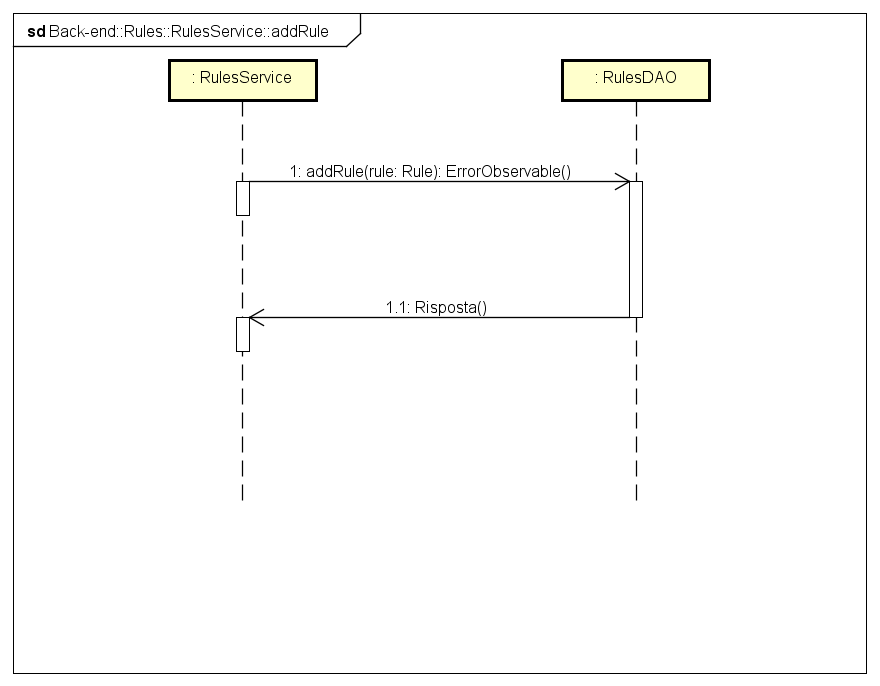
\includegraphics[width=\textwidth,height=\textheight,keepaspectratio]{images/diagrams/back-end/Ufficial_Backend/Back-endRulesRulesServiceaddRule.png} 	\caption{Back-end::Rules::RulesService::addRule}
\end{figure}
\newpage



\subsection{Back-end::Rules::RulesService::getFunction}
Il diagramma qui riportato rappresenta l'implementazione della lambda function che si occupa di ottenere una \file{Function} del sistema attraverso il metodo \file{getFunction}.
 \begin{figure}[h] \centering 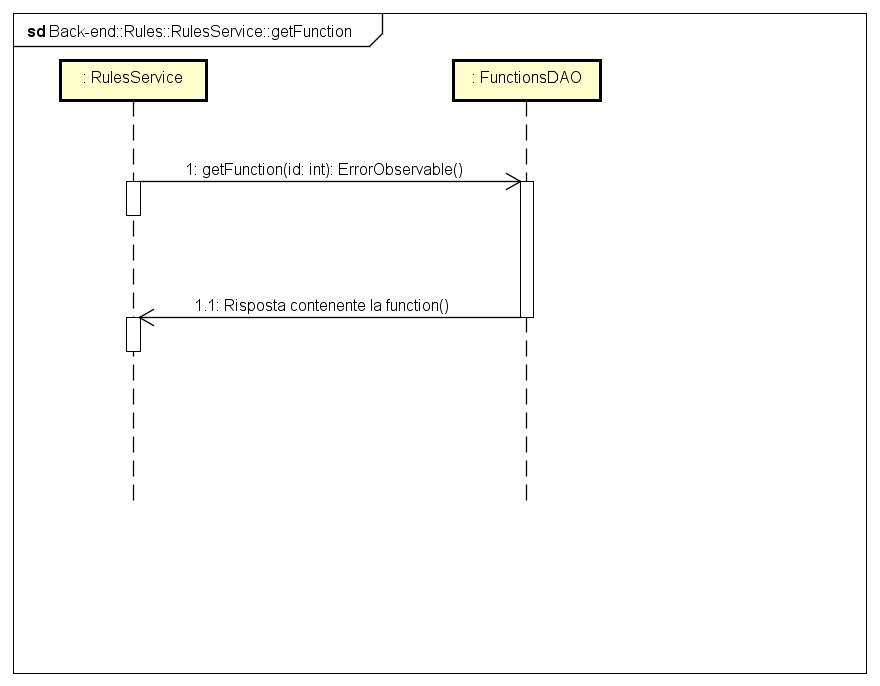
\includegraphics[width=\textwidth,height=\textheight,keepaspectratio]{images/diagrams/back-end/Ufficial_Backend/Back-endRulesRulesServicegetFunction.png} 	\caption{Back-end::Rules::RulesService::getFunction}
\end{figure}
\newpage

\subsection{Back-end::Rules::RulesService::getFunctionList}
Il diagramma qui riportato rappresenta l'implementazione della lambda function che si occupa di ottenere la lista delle \file{Function} del sistema attraverso il metodo \file{getFunctionList}.
 \begin{figure}[h] \centering 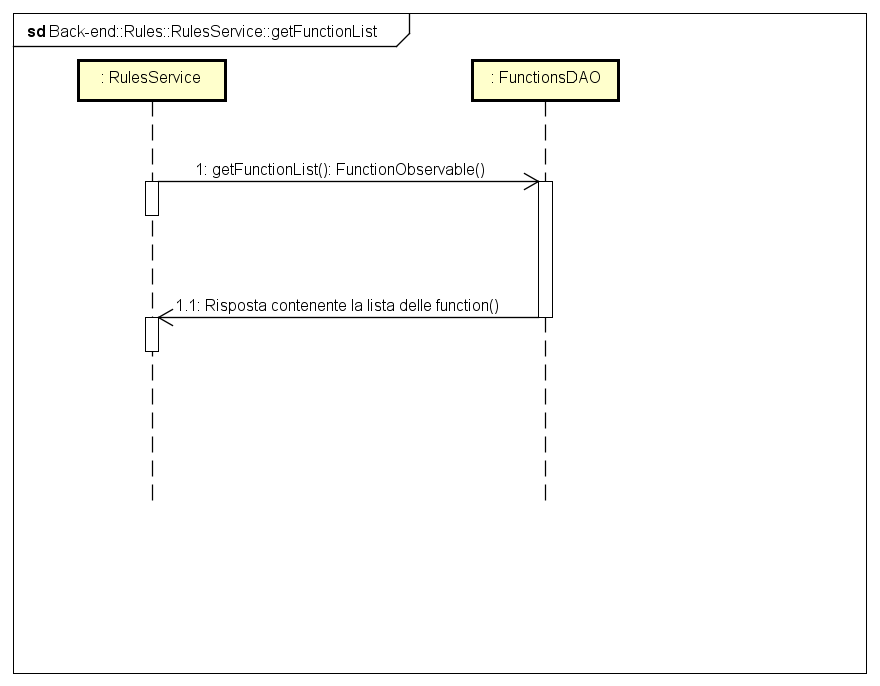
\includegraphics[width=\textwidth,height=\textheight,keepaspectratio]{images/diagrams/back-end/Ufficial_Backend/Back-endRulesRulesServicegetFunctionList.png} 	\caption{Back-end::Rules::RulesService::getFunctionList}
\end{figure}
\newpage

\subsection{Back-end::Rules::RulesService::getRule}
Il diagramma qui riportato rappresenta l'implementazione della lambda function che si occupa di ottenere una \file{Rule} del sistema attraverso il metodo \file{getRule}.
\begin{figure}[h] \centering 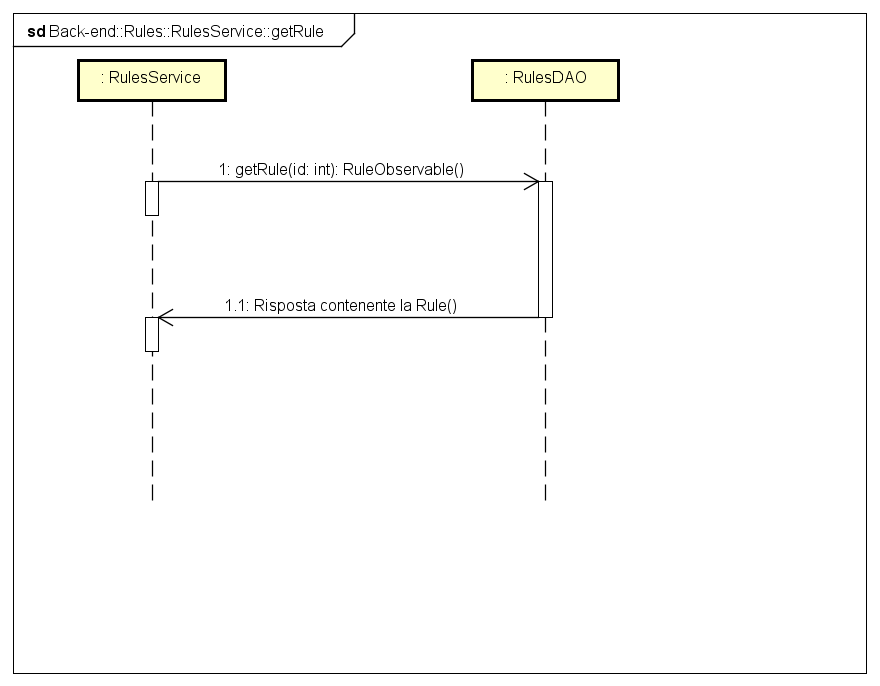
\includegraphics[width=\textwidth,height=\textheight,keepaspectratio]{images/diagrams/back-end/Ufficial_Backend/Back-endRulesRulesServicegetRule.png} 	\caption{Back-end::Rules::RulesService::getRule}
\end{figure}
\newpage

\subsection{Back-end::Rules::RulesService::getRuleList}
Il diagramma qui riportato rappresenta l'implementazione della lambda function che si occupa di ottenere la lista delle \file{Rule} del sistema attraverso il metodo \file{getRuleList}.
\begin{figure}[h] \centering \includegraphics[width=\textwidth,height=\textheight,keepaspectratio]{images/diagrams/back-end/Ufficial_Backend/Back-endRulesRulesServicegetRuleList.png} 	\caption{Back-end::Rules::RulesService::getRuleList}
\end{figure}
\newpage

\subsection{Back-end::Rules::RulesService::deleteRule}
Il diagramma qui riportato rappresenta l'implementazione della lambda function che si occupa di rimuovere una \file{Rule} dal sistema attraverso il metodo \file{deleteRule}.
\begin{figure}[h] \centering \includegraphics[width=\textwidth,height=\textheight,keepaspectratio]{images/diagrams/back-end/Ufficial_Backend/Back-endRulesRulesServicedeleteRule.png} 	\caption{Back-end::Rules::RulesService::deleteRule}
\end{figure}
\newpage

\subsection{Back-end::Rules::RulesService::updateRule}
Il diagramma qui riportato rappresenta l'implementazione della lambda function che si occupa di modificare una \file{Rule} del sistema attraverso il metodo \file{updateRule}.
\begin{figure}[h] \centering \includegraphics[width=\textwidth,height=\textheight,keepaspectratio]{images/diagrams/back-end/Ufficial_Backend/Back-endRulesRulesServiceupdateRule.png} 	\caption{Back-end::Rules::RulesService::updateRule}
\end{figure}
\newpage


\subsection{Back-end::Rules::FunctionsDAODynamoDB::addFunction}
Il diagramma qui riportato rappresenta l'aggiunta di una \file{Function} al database attraverso il metodo \file{put} del \file{DocumentClient} di \file{DynamoDB}, utilizzando la risposta come parametro per chiamare la funzione di callback.
 \begin{figure}[h] \centering \includegraphics[width=\textwidth,height=\textheight,keepaspectratio]{images/diagrams/back-end/Ufficial_Backend/Back-endRulesFunctionsDAODynamoDBaddFunction.png} 	\caption{Back-end::Rules::FunctionsDAODynamoDB::addFunction}
\end{figure}

\newpage
\subsection{Back-end::Rules::FunctionsDAODynamoDB::getFunction}
Il diagramma qui riportato rappresenta l'ottenimento di una \file{Function} dal database attraverso il metodo \file{get} del \file{DocumentClient} di \file{DynamoDB}, utilizzando la risposta come parametro per chiamare la funzione di callback.
\begin{figure}[h] \centering \includegraphics[width=\textwidth,height=\textheight,keepaspectratio]{images/diagrams/back-end/Ufficial_Backend/Back-endRulesFunctionsDAODynamoDBgetFunction.png} 	\caption{Back-end::Rules::FunctionsDAODynamoDB::getFunction}
\end{figure}
\newpage

\subsection{Back-end::Rules::FunctionsDAODynamoDB::getFunctionList}
Il diagramma qui riportato rappresenta l'ottenimento della lista di \file{Function} dal database attraverso il metodo \file{scan} del \file{DocumentClient} di \file{DynamoDB}, utilizzando la risposta come parametro per chiamare la funzione di callback. Poichè il metodo \file{scan} del \file{DocumentClient} permette al più il ritorno di una lista delle dimensioni di 1MB, se il campo LastEvaluetedKey è settato allora non tutte le \file{Function} sono state ritornate, e quindi è necessario rieseguire il metodo scan fornendo come parametro d'ingresso la chiave da cui ripartire per l'estrazione dei dati. Se invece tale campo non è settato allora è stata ritornata l'intera lista.
 \begin{figure}[h] \centering \includegraphics[width=\textwidth,height=\textheight,keepaspectratio]{images/diagrams/back-end/Ufficial_Backend/Back-endRulesFunctionsDAODynamoDBgetFunctionList.png} 	\caption{Back-end::Rules::FunctionsDAODynamoDB::getFunctionList}
\end{figure}
\newpage

\subsection{Back-end::Rules::FunctionsDAODynamoDB::removeFunction}
Il diagramma qui riportato rappresenta la rimozione di una \file{Function} dal database attraverso il metodo \file{delete} del \file{DocumentClient} di \file{DynamoDB}, utilizzando la risposta come parametro per chiamare la funzione di callback.
\begin{figure}[h] \centering \includegraphics[width=\textwidth,height=\textheight,keepaspectratio]{images/diagrams/back-end/Ufficial_Backend/Back-endRulesFunctionsDAODynamoDBremoveFunction.png} 	\caption{Back-end::Rules::FunctionsDAODynamoDB::removeFunction}
\end{figure}
\newpage

\subsection{Back-end::Rules::FunctionsDAODynamoDB::updateFunction}
Il diagramma qui riportato rappresenta la modifica di una \file{Function} del database attraverso il metodo \file{update} del \file{DocumentClient} di \file{DynamoDB}, utilizzando la risposta come parametro per chiamare la funzione di callback.
 \begin{figure}[h] \centering \includegraphics[width=\textwidth,height=\textheight,keepaspectratio]{images/diagrams/back-end/Ufficial_Backend/Back-endRulesFunctionsDAODynamoDBupdateFunction.png} 	\caption{Back-end::Rules::FunctionsDAODynamoDB::updateFunction}
\end{figure}
\newpage

\subsection{Back-end::Rules::RulesDAODynamoDB::addRule}
Il diagramma qui riportato rappresenta l'aggiunta di una \file{Rule} al database attraverso il metodo \file{put} del \file{DocumentClient} di \file{DynamoDB}, utilizzando la risposta come parametro per chiamare la funzione di callback.
\begin{figure}[h] \centering \includegraphics[width=\textwidth,height=\textheight,keepaspectratio]{images/diagrams/back-end/Ufficial_Backend/Back-endRulesRulesDAODynamoDBaddRule.png} 	\caption{Back-end::Rules::RulesDAODynamoDB::addRule}
\end{figure}
\newpage

\subsection{Back-end::Rules::RulesDAODynamoDB::getRule}
Il diagramma qui riportato rappresenta l'ottenimento di una \file{Rule} dal database attraverso il metodo \file{get} del \file{DocumentClient} di \file{DynamoDB}, utilizzando la risposta come parametro per chiamare la funzione di callback.
 \begin{figure}[h] \centering \includegraphics[width=\textwidth,height=\textheight,keepaspectratio]{images/diagrams/back-end/Ufficial_Backend/Back-endRulesRulesDAODynamoDBgetRule.png} 	\caption{Back-end::Rules::RulesDAODynamoDB::getRule}
\end{figure}
\newpage

\subsection{Back-end::Rules::RulesDAODynamoDB::getRuleList}
Il diagramma qui riportato rappresenta l'ottenimento della lista di \file{Rule} dal database attraverso il metodo \file{scan} del \file{DocumentClient} di \file{DynamoDB}, utilizzando la risposta come parametro per chiamare la funzione di callback. Poichè il metodo \file{scan} del \file{DocumentClient} permette al più il ritorno di una lista delle dimensioni di 1MB, se il campo LastEvaluetedKey è settato allora non tutte le \file{Rule} sono state ritornate, e quindi è necessario rieseguire il metodo scan fornendo come parametro d'ingresso la chiave da cui ripartire per l'estrazione dei dati. Se invece tale campo non è settato allora è stata ritornata l'intera lista.
 \begin{figure}[h] \centering \includegraphics[width=\textwidth,height=\textheight,keepaspectratio]{images/diagrams/back-end/Ufficial_Backend/Back-endRulesRulesDAODynamoDBgetRuleList.png} 	\caption{Back-end::Rules::RulesDAODynamoDB::getRuleList}
\end{figure}
\newpage

\subsection{Back-end::Rules::RulesDAODynamoDB::removeRule}
Il diagramma qui riportato rappresenta la rimozione di una \file{Rule} dal database attraverso il metodo \file{delete} del \file{DocumentClient} di \file{DynamoDB}, utilizzando la risposta come parametro per chiamare la funzione di callback.
 \begin{figure}[h] \centering \includegraphics[width=\textwidth,height=\textheight,keepaspectratio]{images/diagrams/back-end/Ufficial_Backend/Back-endRulesRulesDAODynamoDBremoveRule.png} 	\caption{Back-end::Rules::RulesDAODynamoDB::removeRule}
\end{figure}
\newpage

\subsection{Back-end::Rules::RulesDAODynamoDB::updateRule}
Il diagramma qui riportato rappresenta la modifica di una \file{Rule} del database attraverso il metodo \file{update} del \file{DocumentClient} di \file{DynamoDB}, utilizzando la risposta come parametro per chiamare la funzione di callback.
 \begin{figure}[h] \centering \includegraphics[width=\textwidth,height=\textheight,keepaspectratio]{images/diagrams/back-end/Ufficial_Backend/Back-endRulesRulesDAODynamoDBupdateRule.png} 	\caption{Back-end::Rules::RulesDAODynamoDB::updateRule}
\end{figure}
\newpage

\section{Tracciamento}
In questa sezione è riportato il tracciamento dei requisiti in relazione alle classi e alle componenti del \gl{sistema}. Si ricorda che una componente è un insieme di classi raggruppate per scopo, funzionalità o ambito di utilizzo comune. Nel nostro sistema le componenti trovano corrispondenza nei packages.   
\subsection{Tracciamento Classi-Requisiti}
\normalsize
\begin{longtable}{|>{\centering}m{10cm}|m{3cm}<{\centering}|}
\hline 
\textbf{Classe} & \textbf{Requisiti}\\
\hline
\endhead
\hyperref[Back-end::AdministrationWebhookService]{\texttt{Back-end::AdministrationWebhookService}} & RFO1\\
& RFO1.1\\
& RFO1.1.2\\
& RFO1.1.2.1\\
& RFO2.1\\
& RFO2.1.1\\
& RFO2.1.1.1\\
& RFO2.1.1.2\\
& RFO2.1.1.3\\
& RFO2.1.1.3.1\\
& RFO2.1.1.3.2\\
& RFO2.1.1.3.3\\
& RFD2.1.1.4\\
& RFD2.1.1.4.1\\
& RFO2.1.1.5\\
& RFO2.1.1.6\\
& RFO2.1.2\\
& RFO2.1.2.1\\
& RFO2.1.2.2\\
& RFD2.1.2.3\\
& RFD2.1.3\\
& RFD2.1.3.1\\
& RFD2.1.3.2\\
& RFD2.1.3.2.1\\
& RFD2.1.3.2.2\\
& RFD2.1.3.3\\
& RFD2.1.3.4\\
& RFD2.1.3.5\\
& RFD2.1.3.5.1\\
& RFD2.1.3.5.2\\
& RFD2.1.3.5.3\\
& RFD2.1.3.5.4\\
& RFD2.1.3.6\\
& RFD2.1.3.7\\
& RFO2.1.4\\
& RFD2.1.4.1\\
& RFD2.1.4.2\\
& RFO2.1.4.3\\
& RFD2.1.4.4\\
& RFO2.2\\
& RFO2.2.1.1\\
& RFO2.2.3\\
& RFO2.2.4\\
& RFO10\\ \hline

\hyperref[Back-end::APIGateway::Enrollment]{\texttt{Back-end::APIGateway::Enrollment}} & RFO1\\
& RFO1.1\\
& RFO1.1.2\\
& RFO1.1.2.1\\ \hline

\hyperref[Back-end::APIGateway::VocalAPI]{\texttt{Back-end::APIGateway::VocalAPI}} & RFO1\\
& RFO1.1\\
& RFO1.1.1\\
& RFO1.1.1.1\\
& RFO1.1.1.2\\
& RFO1.1.2\\
& RFO1.1.2.1\\
& RFO1.1.3\\
& RFO2\\
& RFO2.1\\
& RFO2.1.1\\
& RFO2.1.1.1\\
& RFO2.1.1.2\\
& RFO2.1.1.3\\
& RFO2.1.1.3.1\\
& RFO2.1.1.3.2\\
& RFO2.1.1.3.3\\
& RFD2.1.1.4\\
& RFD2.1.1.4.1\\
& RFO2.1.1.5\\
& RFO2.1.2\\
& RFO2.1.2.1\\
& RFO2.1.2.2\\
& RFD2.1.2.3\\
& RFD2.1.3\\
& RFD2.1.3.1\\
& RFD2.1.3.2\\
& RFD2.1.3.2.1\\
& RFD2.1.3.2.2\\
& RFD2.1.3.3\\
& RFD2.1.3.4\\
& RFD2.1.3.5\\
& RFD2.1.3.5.1\\
& RFD2.1.3.5.2\\
& RFD2.1.3.5.3\\
& RFD2.1.3.5.4\\
& RFD2.1.3.6\\
& RFO2.1.4\\
& RFD2.1.4.1\\
& RFD2.1.4.2\\
& RFO2.1.4.3\\
& RFD2.1.4.4\\
& RFO2.2\\
& RFO2.2.1\\
& RFO2.2.1.1\\
& RFO2.2.3\\
& RFO3\\
& RFO3.1\\
& RFD3.2\\
& RFD3.2.1\\
& RFD3.2.2\\
& RFD3.2.3\\
& RFD3.2.3.1\\
& RFD3.2.3.2\\
& RFD3.2.4\\
& RFD3.3\\
& RFD3.3.2\\
& RFD3.3.2.1\\ \hline

\hyperref[Back-end::APIGateway::VocalLoginModuleConfig]{\texttt{Back-end::APIGateway::-\linebreak VocalLoginModuleConfig}} & RFO1\\
& RFO1.1\\
& RFO1.1.2\\
& RFO1.1.2.1\\ \hline

\hyperref[Back-end::Conversations::<<interface>> ConversationsDAO]{\texttt{Back-end::Conversations::-\linebreak <<interface>> ConversationsDAO}} & RFO7.1\\ \hline

\hyperref[Back-end::Conversations::Conversation]{\texttt{Back-end::Conversations::Conversation}} & RFO7.1\\ \hline

\hyperref[Back-end::Conversations::ConversationMsg]{\texttt{Back-end::Conversations::-\linebreak ConversationMsg}} & RFO7.1\\ \hline

\hyperref[Back-end::Conversations::ConversationObservable]{\texttt{Back-end::Conversations::-\linebreak ConversationObservable}} & RFO7.1\\ \hline

\hyperref[Back-end::Conversations::ConversationObserver]{\texttt{Back-end::Conversations::-\linebreak ConversationObserver}} & RFO7.1\\ \hline

\hyperref[Back-end::Conversations::ConversationsDAODynamoDB]{\texttt{Back-end::Conversations::-\linebreak ConversationsDAODynamoDB}} & RFO7.1\\
& RVO3.1\\ \hline

\hyperref[Back-end::ConversationWebhookService]{\texttt{Back-end::ConversationWebhookService}} & RFO7\\
& RFO7.1\\
& RFO7.2\\ \hline

\hyperref[Back-end::Events::SNSMessage]{\texttt{Back-end::Events::SNSMessage}} & RFO12\\
& RFO12.1\\
& RFO12.1.1\\
& RFO12.1.2\\
& RFO12.2\\
& RFO12.3\\
& RFD12.4\\
& RFD12.5\\ \hline

\hyperref[Back-end::Events::SNSRecord]{\texttt{Back-end::Events::SNSRecord}} & RFO12\\
& RFO12.1\\
& RFO12.1.1\\
& RFO12.1.2\\
& RFO12.2\\
& RFO12.3\\
& RFD12.4\\
& RFD12.5\\ \hline

\hyperref[Back-end::Events::VAMessageListener]{\texttt{Back-end::Events::VAMessageListener}} & RFO7\\
& RFO7.1\\
& RFO7.2\\
& RFO10\\
& RFD11\\
& RFO12\\
& RFO12.1\\
& RFO12.1.1\\
& RFO12.1.2\\
& RFO12.2\\
& RFO12.3\\
& RFD12.4\\
& RFD12.5\\ \hline

\hyperref[Back-end::Guests::<<interface>> GuestsDAO]{\texttt{Back-end::Guests::-\linebreak <<interface>> GuestsDAO}} & RFO7\\
& RFO7.1\\
& RFO7.2\\
& RFO10\\
& RFD11\\
& RFO12\\
& RFO12.1\\
& RFO12.1.1\\
& RFO12.1.2\\
& RFO12.2\\
& RFO12.3\\
& RFD12.4\\
& RFD12.5\\ \hline

\hyperref[Back-end::Guests::Guest]{\texttt{Back-end::Guests::Guest}} & RFO7\\
& RFO7.1\\
& RFO7.2\\
& RFO10\\
& RFD11\\
& RFO12\\
& RFO12.1\\
& RFO12.1.1\\
& RFO12.1.2\\
& RFO12.2\\
& RFO12.3\\
& RFD12.4\\
& RFD12.5\\ \hline

\hyperref[Back-end::Guests::GuestObservable]{\texttt{Back-end::Guests::GuestObservable}} & RFO7\\
& RFO7.1\\
& RFO7.2\\
& RFO10\\
& RFD11\\
& RFO12\\
& RFO12.1\\
& RFO12.1.1\\
& RFO12.1.2\\
& RFO12.2\\
& RFO12.3\\
& RFD12.4\\
& RFD12.5\\ \hline

\hyperref[Back-end::Guests::GuestObserver]{\texttt{Back-end::Guests::GuestObserver}} & RFO7\\
& RFO7.1\\
& RFO7.2\\
& RFO10\\
& RFD11\\
& RFO12\\
& RFO12.1\\
& RFO12.1.1\\
& RFO12.1.2\\
& RFO12.2\\
& RFO12.3\\
& RFD12.4\\
& RFD12.5\\ \hline

\hyperref[Back-end::Guests::GuestsDAODynamoDB]{\texttt{Back-end::Guests::GuestsDAODynamoDB}} & RFO7\\
& RFO7.1\\
& RFO7.2\\
& RFO10\\
& RFD11\\
& RFO12\\
& RFO12.1\\
& RFO12.1.1\\
& RFO12.1.2\\
& RFO12.2\\
& RFO12.3\\
& RFD12.4\\
& RFD12.5\\
& RVO3.1\\ \hline

\hyperref[Back-end::Members::<<interface>> MembersDAO]{\texttt{Back-end::Members::-\linebreak <<interface>> MembersDAO}} & RFO13\\ \hline

\hyperref[Back-end::Members::Member]{\texttt{Back-end::Members::Member}} & RFO13\\ \hline

\hyperref[Back-end::Members::MemberObservable]{\texttt{Back-end::Members::MemberObservable}} & RFO13\\ \hline

\hyperref[Back-end::Members::MemberObserver]{\texttt{Back-end::Members::MemberObserver}} & RFO13\\ \hline

\hyperref[Back-end::Members::MembersDAOSlack]{\texttt{Back-end::Members::MembersDAOSlack}} & RFO13\\ \hline

\hyperref[Back-end::Notifications::Action]{\texttt{Back-end::Notifications::Action}} & RFO13\\
& RFO13.1\\
& RFD13.2\\ \hline

\hyperref[Back-end::Notifications::Attachment]{\texttt{Back-end::Notifications::Attachment}} & RFO13\\
& RFO13.1\\
& RFD13.2\\ \hline

\hyperref[Back-end::Notifications::ConfirmationFields]{\texttt{Back-end::Notifications::-\linebreak ConfirmationFields}} & RFO13\\
& RFO13.1\\
& RFD13.2\\ \hline

\hyperref[Back-end::Notifications::NotificationChannel]{\texttt{Back-end::Notifications::-\linebreak NotificationChannel}} & RFO13\\
& RFO13.1\\
& RFD13.2\\ \hline

\hyperref[Back-end::Notifications::NotificationMessage]{\texttt{Back-end::Notifications::-\linebreak NotificationMessage}} & RFO13\\
& RFO13.1\\
& RFD13.2\\ \hline

\hyperref[Back-end::Notifications::NotificationService]{\texttt{Back-end::Notifications::-\linebreak NotificationService}} & RFO13\\
& RFO13.1\\
& RFD13.2\\ \hline

\hyperref[Back-end::Rules::<<interface>> RulesDAO]{\texttt{Back-end::Rules::-\linebreak <<interface>> RulesDAO}} & RFO2.1\\
& RFO2.1.1\\
& RFO2.1.1.1\\
& RFO2.1.1.1.1\\
& RFO2.1.1.2\\
& RFO2.1.1.3\\
& RFO2.1.1.3.1\\
& RFO2.1.1.3.2\\
& RFO2.1.1.3.3\\
& RFD2.1.1.4\\
& RFD2.1.1.4.1\\
& RFO2.1.1.5\\
& RFO2.1.1.6\\
& RFO2.1.2\\
& RFO2.1.2.1\\
& RFO2.1.2.2\\
& RFD2.1.2.3\\
& RFD2.1.3\\
& RFD2.1.3.1\\
& RFD2.1.3.2\\
& RFD2.1.3.2.1\\
& RFD2.1.3.2.2\\
& RFD2.1.3.3\\
& RFD2.1.3.4\\
& RFD2.1.3.5\\
& RFD2.1.3.5.1\\
& RFD2.1.3.5.2\\
& RFD2.1.3.5.3\\
& RFD2.1.3.5.4\\
& RFD2.1.3.6\\
& RFD2.1.3.7\\
& RFO2.1.4\\
& RFD2.1.4.1\\
& RFD2.1.4.2\\
& RFO2.1.4.3\\
& RFD2.1.4.4\\ \hline

\hyperref[Back-end::Rules::<<interface>> TasksDAO]{\texttt{Back-end::Rules::-\linebreak <<interface>> TasksDAO}} & RFO2.1.1.1\\
& RFO2.1.1.1.1\\
& RFD2.1.3.3\\
& RFO2.1.4.3\\
& RFO4\\
& RFO10\\ \hline

\hyperref[Back-end::Rules::Rule]{\texttt{Back-end::Rules::Rule}} & RFO2.1\\
& RFO2.1.1\\
& RFO2.1.1.1\\
& RFO2.1.1.1.1\\
& RFO2.1.1.2\\
& RFO2.1.1.3\\
& RFO2.1.1.3.1\\
& RFO2.1.1.3.2\\
& RFO2.1.1.3.3\\
& RFD2.1.1.4\\
& RFD2.1.1.4.1\\
& RFO2.1.1.5\\
& RFO2.1.1.6\\
& RFO2.1.2\\
& RFO2.1.2.1\\
& RFO2.1.2.2\\
& RFD2.1.2.3\\
& RFD2.1.3\\
& RFD2.1.3.1\\
& RFD2.1.3.2\\
& RFD2.1.3.2.1\\
& RFD2.1.3.2.2\\
& RFD2.1.3.3\\
& RFD2.1.3.4\\
& RFD2.1.3.5\\
& RFD2.1.3.5.1\\
& RFD2.1.3.5.2\\
& RFD2.1.3.5.3\\
& RFD2.1.3.5.4\\
& RFD2.1.3.6\\
& RFD2.1.3.7\\
& RFO2.1.4\\
& RFD2.1.4.1\\
& RFD2.1.4.2\\
& RFO2.1.4.3\\
& RFD2.1.4.4\\ \hline

\hyperref[Back-end::Rules::RuleObservable]{\texttt{Back-end::Rules::RuleObservable}} & RFO2.1\\
& RFO2.1.1\\
& RFO2.1.1.1\\
& RFO2.1.1.1.1\\
& RFO2.1.1.2\\
& RFO2.1.1.3\\
& RFO2.1.1.3.1\\
& RFO2.1.1.3.2\\
& RFO2.1.1.3.3\\
& RFD2.1.1.4\\
& RFD2.1.1.4.1\\
& RFO2.1.1.5\\
& RFO2.1.1.6\\
& RFO2.1.2\\
& RFO2.1.2.1\\
& RFO2.1.2.2\\
& RFD2.1.2.3\\
& RFD2.1.3\\
& RFD2.1.3.1\\
& RFD2.1.3.2\\
& RFD2.1.3.2.1\\
& RFD2.1.3.2.2\\
& RFD2.1.3.3\\
& RFD2.1.3.4\\
& RFD2.1.3.5\\
& RFD2.1.3.5.1\\
& RFD2.1.3.5.2\\
& RFD2.1.3.5.3\\
& RFD2.1.3.5.4\\
& RFD2.1.3.6\\
& RFD2.1.3.7\\
& RFO2.1.4\\
& RFD2.1.4.1\\
& RFD2.1.4.2\\
& RFO2.1.4.3\\
& RFD2.1.4.4\\ \hline

\hyperref[Back-end::Rules::RuleObserver]{\texttt{Back-end::Rules::RuleObserver}} & RFO2.1\\
& RFO2.1.1\\
& RFO2.1.1.1\\
& RFO2.1.1.1.1\\
& RFO2.1.1.2\\
& RFO2.1.1.3\\
& RFO2.1.1.3.1\\
& RFO2.1.1.3.2\\
& RFO2.1.1.3.3\\
& RFD2.1.1.4\\
& RFD2.1.1.4.1\\
& RFO2.1.1.5\\
& RFO2.1.1.6\\
& RFO2.1.2\\
& RFO2.1.2.1\\
& RFO2.1.2.2\\
& RFD2.1.2.3\\
& RFD2.1.3\\
& RFD2.1.3.1\\
& RFD2.1.3.2\\
& RFD2.1.3.2.1\\
& RFD2.1.3.2.2\\
& RFD2.1.3.3\\
& RFD2.1.3.4\\
& RFD2.1.3.5\\
& RFD2.1.3.5.1\\
& RFD2.1.3.5.2\\
& RFD2.1.3.5.3\\
& RFD2.1.3.5.4\\
& RFD2.1.3.6\\
& RFD2.1.3.7\\
& RFO2.1.4\\
& RFD2.1.4.1\\
& RFD2.1.4.2\\
& RFO2.1.4.3\\
& RFD2.1.4.4\\ \hline

\hyperref[Back-end::Rules::RulesDAODynamoDB]{\texttt{Back-end::Rules::RulesDAODynamoDB}} & RFO2.1\\
& RFO2.1.1\\
& RFO2.1.1.1\\
& RFO2.1.1.1.1\\
& RFO2.1.1.2\\
& RFO2.1.1.3\\
& RFO2.1.1.3.1\\
& RFO2.1.1.3.2\\
& RFO2.1.1.3.3\\
& RFD2.1.1.4\\
& RFD2.1.1.4.1\\
& RFO2.1.1.5\\
& RFO2.1.1.6\\
& RFO2.1.2\\
& RFO2.1.2.1\\
& RFO2.1.2.2\\
& RFD2.1.2.3\\
& RFD2.1.3\\
& RFD2.1.3.1\\
& RFD2.1.3.2\\
& RFD2.1.3.2.1\\
& RFD2.1.3.2.2\\
& RFD2.1.3.3\\
& RFD2.1.3.4\\
& RFD2.1.3.5\\
& RFD2.1.3.5.1\\
& RFD2.1.3.5.2\\
& RFD2.1.3.5.3\\
& RFD2.1.3.5.4\\
& RFD2.1.3.6\\
& RFD2.1.3.7\\
& RFO2.1.4\\
& RFD2.1.4.1\\
& RFD2.1.4.2\\
& RFO2.1.4.3\\
& RFD2.1.4.4\\
& RVO3.1\\ \hline

\hyperref[Back-end::Rules::RulesService]{\texttt{Back-end::Rules::RulesService}} & RFO2.1\\
& RFO2.1.1\\
& RFO2.1.1.1\\
& RFO2.1.1.1.1\\
& RFO2.1.1.2\\
& RFO2.1.1.3\\
& RFO2.1.1.3.1\\
& RFO2.1.1.3.2\\
& RFO2.1.1.3.3\\
& RFD2.1.1.4\\
& RFD2.1.1.4.1\\
& RFO2.1.1.5\\
& RFO2.1.1.6\\
& RFO2.1.2\\
& RFO2.1.2.1\\
& RFO2.1.2.2\\
& RFD2.1.2.3\\
& RFD2.1.3\\
& RFD2.1.3.1\\
& RFD2.1.3.2\\
& RFD2.1.3.2.1\\
& RFD2.1.3.2.2\\
& RFD2.1.3.3\\
& RFD2.1.3.4\\
& RFD2.1.3.5\\
& RFD2.1.3.5.1\\
& RFD2.1.3.5.2\\
& RFD2.1.3.5.3\\
& RFD2.1.3.5.4\\
& RFD2.1.3.6\\
& RFD2.1.3.7\\
& RFO2.1.4\\
& RFD2.1.4.1\\
& RFD2.1.4.2\\
& RFO2.1.4.3\\
& RFD2.1.4.4\\ \hline

\hyperref[Back-end::Rules::RuleTarget]{\texttt{Back-end::Rules::RuleTarget}} & RFO2.1.1.3\\
& RFO2.1.1.3.1\\
& RFO2.1.1.3.2\\
& RFO2.1.1.3.3\\
& RFD2.1.3.2\\
& RFD2.1.3.2.1\\
& RFD2.1.3.2.2\\
& RFD2.1.4.2\\
& RFO10\\ \hline

\hyperref[Back-end::Rules::RuleTaskInstance]{\texttt{Back-end::Rules::RuleTaskInstance}} & RFO2.1.1.1\\
& RFO2.1.1.1.1\\
& RFD2.1.3.3\\
& RFO2.1.4.3\\
& RFO4\\
& RFO10\\ \hline

\hyperref[Back-end::Rules::Task]{\texttt{Back-end::Rules::Task}} & RFO2.1.1.1\\
& RFO2.1.1.1.1\\
& RFD2.1.3.3\\
& RFO2.1.4.3\\
& RFO4\\
& RFO10\\ \hline

\hyperref[Back-end::Rules::TaskObservable]{\texttt{Back-end::Rules::TaskObservable}} & RFO2.1.1.1\\
& RFO2.1.1.1.1\\
& RFD2.1.3.3\\
& RFO2.1.4.3\\
& RFO4\\
& RFO10\\ \hline

\hyperref[Back-end::Rules::TaskObserver]{\texttt{Back-end::Rules::TaskObserver}} & RFO2.1.1.1\\
& RFO2.1.1.1.1\\
& RFD2.1.3.3\\
& RFO2.1.4.3\\
& RFO4\\
& RFO10\\ \hline

\hyperref[Back-end::Rules::TasksDAODynamoDB]{\texttt{Back-end::Rules::TasksDAODynamoDB}} & RFO2.1.1.1\\
& RFO2.1.1.1.1\\
& RFD2.1.3.3\\
& RFO2.1.4.3\\
& RFO4\\
& RFO10\\
& RVO3.1\\ \hline

\hyperref[Back-end::SNSEvent]{\texttt{Back-end::SNSEvent}} & RFO12\\
& RFO12.1\\
& RFO12.1.1\\
& RFO12.1.2\\
& RFO12.2\\
& RFO12.3\\
& RFD12.4\\
& RFD12.5\\ \hline

\hyperref[Back-end::STT::<<interface>> STTModule]{\texttt{Back-end::STT::<<interface>> STTModule}} & RFO1\\
& RFO1.1\\
& RFO1.1.1\\
& RFO1.1.1.1\\
& RFO1.1.1.2\\
& RFO1.1.2\\
& RFO1.1.3\\
& RFO2\\
& RFO2.1\\
& RFO2.1.1\\
& RFO2.1.1.1\\
& RFO2.1.1.1.1\\
& RFO2.1.1.2\\
& RFO2.1.1.3\\
& RFO2.1.1.3.1\\
& RFO2.1.1.3.2\\
& RFO2.1.1.3.3\\
& RFD2.1.1.4\\
& RFD2.1.1.4.1\\
& RFO2.1.1.5\\
& RFO2.1.1.6\\
& RFO2.1.2\\
& RFO2.1.2.1\\
& RFO2.1.2.2\\
& RFD2.1.2.3\\
& RFD2.1.3\\
& RFD2.1.3.1\\
& RFD2.1.3.2\\
& RFD2.1.3.2.1\\
& RFD2.1.3.2.2\\
& RFD2.1.3.3\\
& RFD2.1.3.4\\
& RFD2.1.3.5\\
& RFD2.1.3.5.1\\
& RFD2.1.3.5.2\\
& RFD2.1.3.5.3\\
& RFD2.1.3.5.4\\
& RFD2.1.3.6\\
& RFD2.1.3.7\\
& RFO2.1.4\\
& RFD2.1.4.1\\
& RFD2.1.4.2\\
& RFO2.1.4.3\\
& RFD2.1.4.4\\
& RFO2.2\\
& RFO2.2.1\\
& RFO2.2.1.1\\
& RFO2.2.3\\
& RFO2.2.4\\
& RFO3\\
& RFO3.1\\
& RFD3.2\\
& RFD3.2.1\\
& RFD3.2.2\\
& RFD3.2.3\\
& RFD3.2.3.1\\
& RFD3.2.3.2\\
& RFD3.2.3.3\\
& RFD3.2.4\\
& RFD3.3\\
& RFD3.3.2\\
& RFD3.3.2.1\\ \hline

\hyperref[Back-end::STT::STTWatsonAdapter]{\texttt{Back-end::STT::STTWatsonAdapter}} & RFO1\\
& RFO1.1\\
& RFO1.1.1\\
& RFO1.1.1.1\\
& RFO1.1.1.2\\
& RFO1.1.2\\
& RFO1.1.3\\
& RFO2\\
& RFO2.1\\
& RFO2.1.1\\
& RFO2.1.1.1\\
& RFO2.1.1.1.1\\
& RFO2.1.1.2\\
& RFO2.1.1.3\\
& RFO2.1.1.3.1\\
& RFO2.1.1.3.2\\
& RFO2.1.1.3.3\\
& RFD2.1.1.4\\
& RFD2.1.1.4.1\\
& RFO2.1.1.5\\
& RFO2.1.1.6\\
& RFO2.1.2\\
& RFO2.1.2.1\\
& RFO2.1.2.2\\
& RFD2.1.2.3\\
& RFD2.1.3\\
& RFD2.1.3.1\\
& RFD2.1.3.2\\
& RFD2.1.3.2.1\\
& RFD2.1.3.2.2\\
& RFD2.1.3.3\\
& RFD2.1.3.4\\
& RFD2.1.3.5\\
& RFD2.1.3.5.1\\
& RFD2.1.3.5.2\\
& RFD2.1.3.5.3\\
& RFD2.1.3.5.4\\
& RFD2.1.3.6\\
& RFD2.1.3.7\\
& RFO2.1.4\\
& RFD2.1.4.1\\
& RFD2.1.4.2\\
& RFO2.1.4.3\\
& RFD2.1.4.4\\
& RFO2.2\\
& RFO2.2.1\\
& RFO2.2.1.1\\
& RFO2.2.3\\
& RFO2.2.4\\
& RFO3\\
& RFO3.1\\
& RFD3.2\\
& RFD3.2.1\\
& RFD3.2.2\\
& RFD3.2.3\\
& RFD3.2.3.1\\
& RFD3.2.3.2\\
& RFD3.2.3.3\\
& RFD3.2.4\\
& RFD3.3\\
& RFD3.3.2\\
& RFD3.3.2.1\\ \hline

\hyperref[Back-end::Users::<<interface>> UsersDAO]{\texttt{Back-end::Users::-\linebreak <<interface>> UsersDAO}} & RFO2\\
& RFO2.2\\
& RFO2.2.1\\
& RFO2.2.1.1\\
& RFO2.2.3\\
& RFO2.2.4\\ \hline

\hyperref[Back-end::Users::<<interface>>VocalLoginModule]{\texttt{Back-end::Users::-\linebreak <<interface>>VocalLoginModule}} & RFO1\\
& RFO1.1.2\\
& RFO1.1.2.1\\ \hline

\hyperref[Back-end::Users::SRUser]{\texttt{Back-end::Users::SRUser}} & RFO1\\
& RFO1.1.2\\
& RFO1.1.2.1\\ \hline

\hyperref[Back-end::Users::User]{\texttt{Back-end::Users::User}} & RFO2\\
& RFO2.2\\
& RFO2.2.1\\
& RFO2.2.1.1\\
& RFO2.2.3\\
& RFO2.2.4\\ \hline

\hyperref[Back-end::Users::UserObservable]{\texttt{Back-end::Users::UserObservable}} & RFO2\\
& RFO2.2\\
& RFO2.2.1\\
& RFO2.2.1.1\\
& RFO2.2.3\\
& RFO2.2.4\\ \hline

\hyperref[Back-end::Users::UserObserver]{\texttt{Back-end::Users::UserObserver}} & RFO2\\
& RFO2.2\\
& RFO2.2.1\\
& RFO2.2.1.1\\
& RFO2.2.3\\
& RFO2.2.4\\ \hline

\hyperref[Back-end::Users::UsersDAODynamoDB]{\texttt{Back-end::Users::UsersDAODynamoDB}} & RFO2\\
& RFO2.2\\
& RFO2.2.1\\
& RFO2.2.1.1\\
& RFO2.2.3\\
& RFO2.2.4\\
& RVO3.1\\ \hline

\hyperref[Back-end::Users::UsersService]{\texttt{Back-end::Users::UsersService}} & RFO2\\
& RFO2.2\\
& RFO2.2.1\\
& RFO2.2.1.1\\
& RFO2.2.3\\
& RFO2.2.4\\ \hline

\hyperref[Back-end::Users::VocalLoginMicrosoftModule]{\texttt{Back-end::Users::-\linebreak VocalLoginMicrosoftModule}} & RFO1\\
& RFO1.1.2\\
& RFO1.1.2.1\\ \hline

\hyperref[Back-end::Utility::LambdaContext]{\texttt{Back-end::Utility::LambdaContext}} & RFO1\\
& RFO1.1\\
& RFO1.1.1\\
& RFO1.1.1.1\\
& RFO1.1.1.2\\
& RFO1.1.2\\
& RFO1.1.2.1\\
& RFO1.1.3\\
& RFO2\\
& RFO2.1\\
& RFO2.1.1\\
& RFO2.1.1.1\\
& RFO2.1.1.1.1\\
& RFO2.1.1.2\\
& RFO2.1.1.3\\
& RFO2.1.1.3.1\\
& RFO2.1.1.3.2\\
& RFO2.1.1.3.3\\
& RFD2.1.1.4\\
& RFD2.1.1.4.1\\
& RFO2.1.1.5\\
& RFO2.1.1.6\\
& RFO2.1.2\\
& RFO2.1.2.1\\
& RFO2.1.2.2\\
& RFD2.1.2.3\\
& RFD2.1.3\\
& RFD2.1.3.1\\
& RFD2.1.3.2\\
& RFD2.1.3.2.1\\
& RFD2.1.3.2.2\\
& RFD2.1.3.3\\
& RFD2.1.3.4\\
& RFD2.1.3.5\\
& RFD2.1.3.5.1\\
& RFD2.1.3.5.2\\
& RFD2.1.3.5.3\\
& RFD2.1.3.5.4\\
& RFD2.1.3.6\\
& RFD2.1.3.7\\
& RFO2.1.4\\
& RFD2.1.4.1\\
& RFD2.1.4.2\\
& RFO2.1.4.3\\
& RFD2.1.4.4\\
& RFO2.2\\
& RFO2.2.1\\
& RFO2.2.1.1\\
& RFO2.2.3\\
& RFO2.2.4\\
& RFO3\\
& RFO3.1\\
& RFD3.2\\
& RFD3.2.1\\
& RFD3.2.2\\
& RFD3.2.3\\
& RFD3.2.3.1\\
& RFD3.2.3.2\\
& RFD3.2.3.3\\
& RFD3.2.4\\
& RFD3.3\\
& RFD3.3.2\\
& RFD3.3.2.1\\ \hline

\hyperref[Back-end::Utility::LambdaEvent]{\texttt{Back-end::Utility::LambdaEvent}} & RFO1\\
& RFO1.1\\
& RFO1.1.1\\
& RFO1.1.1.1\\
& RFO1.1.1.2\\
& RFO1.1.2\\
& RFO1.1.2.1\\
& RFO1.1.3\\
& RFO2\\
& RFO2.1\\
& RFO2.1.1\\
& RFO2.1.1.1\\
& RFO2.1.1.1.1\\
& RFO2.1.1.2\\
& RFO2.1.1.3\\
& RFO2.1.1.3.1\\
& RFO2.1.1.3.2\\
& RFO2.1.1.3.3\\
& RFD2.1.1.4\\
& RFD2.1.1.4.1\\
& RFO2.1.1.5\\
& RFO2.1.1.6\\
& RFO2.1.2\\
& RFO2.1.2.1\\
& RFO2.1.2.2\\
& RFD2.1.2.3\\
& RFD2.1.3\\
& RFD2.1.3.1\\
& RFD2.1.3.2\\
& RFD2.1.3.2.1\\
& RFD2.1.3.2.2\\
& RFD2.1.3.3\\
& RFD2.1.3.4\\
& RFD2.1.3.5\\
& RFD2.1.3.5.1\\
& RFD2.1.3.5.2\\
& RFD2.1.3.5.3\\
& RFD2.1.3.5.4\\
& RFD2.1.3.6\\
& RFD2.1.3.7\\
& RFO2.1.4\\
& RFD2.1.4.1\\
& RFD2.1.4.2\\
& RFO2.1.4.3\\
& RFD2.1.4.4\\
& RFO2.2\\
& RFO2.2.1\\
& RFO2.2.1.1\\
& RFO2.2.3\\
& RFO2.2.4\\
& RFO3\\
& RFO3.1\\
& RFD3.2\\
& RFD3.2.1\\
& RFD3.2.2\\
& RFD3.2.3\\
& RFD3.2.3.1\\
& RFD3.2.3.2\\
& RFD3.2.3.3\\
& RFD3.2.4\\
& RFD3.3\\
& RFD3.3.2\\
& RFD3.3.2.1\\ \hline

\hyperref[Back-end::Utility::LambdaIdEvent]{\texttt{Back-end::Utility::LambdaIdEvent}} & RFO1\\
& RFO1.1\\
& RFO1.1.1\\
& RFO1.1.1.1\\
& RFO1.1.1.2\\
& RFO1.1.2\\
& RFO1.1.2.1\\
& RFO1.1.3\\
& RFO2\\
& RFO2.1\\
& RFO2.1.1\\
& RFO2.1.1.1\\
& RFO2.1.1.1.1\\
& RFO2.1.1.2\\
& RFO2.1.1.3\\
& RFO2.1.1.3.1\\
& RFO2.1.1.3.2\\
& RFO2.1.1.3.3\\
& RFD2.1.1.4\\
& RFD2.1.1.4.1\\
& RFO2.1.1.5\\
& RFO2.1.1.6\\
& RFO2.1.2\\
& RFO2.1.2.1\\
& RFO2.1.2.2\\
& RFD2.1.2.3\\
& RFD2.1.3\\
& RFD2.1.3.1\\
& RFD2.1.3.2\\
& RFD2.1.3.2.1\\
& RFD2.1.3.2.2\\
& RFD2.1.3.3\\
& RFD2.1.3.4\\
& RFD2.1.3.5\\
& RFD2.1.3.5.1\\
& RFD2.1.3.5.2\\
& RFD2.1.3.5.3\\
& RFD2.1.3.5.4\\
& RFD2.1.3.6\\
& RFD2.1.3.7\\
& RFO2.1.4\\
& RFD2.1.4.1\\
& RFD2.1.4.2\\
& RFO2.1.4.3\\
& RFD2.1.4.4\\
& RFO2.2\\
& RFO2.2.1\\
& RFO2.2.1.1\\
& RFO2.2.3\\
& RFO2.2.4\\
& RFO3\\
& RFO3.1\\
& RFD3.2\\
& RFD3.2.1\\
& RFD3.2.2\\
& RFD3.2.3\\
& RFD3.2.3.1\\
& RFD3.2.3.2\\
& RFD3.2.3.3\\
& RFD3.2.4\\
& RFD3.3\\
& RFD3.3.2\\
& RFD3.3.2.1\\ \hline

\hyperref[Back-end::Utility::LambdaResponse]{\texttt{Back-end::Utility::LambdaResponse}} & RFO1\\
& RFO1.1\\
& RFO1.1.1\\
& RFO1.1.1.1\\
& RFO1.1.1.2\\
& RFO1.1.2\\
& RFO1.1.2.1\\
& RFO1.1.3\\
& RFO2\\
& RFO2.1\\
& RFO2.1.1\\
& RFO2.1.1.1\\
& RFO2.1.1.1.1\\
& RFO2.1.1.2\\
& RFO2.1.1.3\\
& RFO2.1.1.3.1\\
& RFO2.1.1.3.2\\
& RFO2.1.1.3.3\\
& RFD2.1.1.4\\
& RFD2.1.1.4.1\\
& RFO2.1.1.5\\
& RFO2.1.1.6\\
& RFO2.1.2\\
& RFO2.1.2.1\\
& RFO2.1.2.2\\
& RFD2.1.2.3\\
& RFD2.1.3\\
& RFD2.1.3.1\\
& RFD2.1.3.2\\
& RFD2.1.3.2.1\\
& RFD2.1.3.2.2\\
& RFD2.1.3.3\\
& RFD2.1.3.4\\
& RFD2.1.3.5\\
& RFD2.1.3.5.1\\
& RFD2.1.3.5.2\\
& RFD2.1.3.5.3\\
& RFD2.1.3.5.4\\
& RFD2.1.3.6\\
& RFD2.1.3.7\\
& RFO2.1.4\\
& RFD2.1.4.1\\
& RFD2.1.4.2\\
& RFO2.1.4.3\\
& RFD2.1.4.4\\
& RFO2.2\\
& RFO2.2.1\\
& RFO2.2.1.1\\
& RFO2.2.3\\
& RFO2.2.4\\
& RFO3\\
& RFO3.1\\
& RFD3.2\\
& RFD3.2.1\\
& RFD3.2.2\\
& RFD3.2.3\\
& RFD3.2.3.1\\
& RFD3.2.3.2\\
& RFD3.2.3.3\\
& RFD3.2.4\\
& RFD3.3\\
& RFD3.3.2\\
& RFD3.3.2.1\\ \hline

\hyperref[Back-end::Utility::PathIdParam]{\texttt{Back-end::Utility::PathIdParam}} & RFO1\\
& RFO1.1\\
& RFO1.1.1\\
& RFO1.1.1.1\\
& RFO1.1.1.2\\
& RFO1.1.2\\
& RFO1.1.2.1\\
& RFO1.1.3\\
& RFO2\\
& RFO2.1\\
& RFO2.1.1\\
& RFO2.1.1.1\\
& RFO2.1.1.1.1\\
& RFO2.1.1.2\\
& RFO2.1.1.3\\
& RFO2.1.1.3.1\\
& RFO2.1.1.3.2\\
& RFO2.1.1.3.3\\
& RFD2.1.1.4\\
& RFD2.1.1.4.1\\
& RFO2.1.1.5\\
& RFO2.1.1.6\\
& RFO2.1.2\\
& RFO2.1.2.1\\
& RFO2.1.2.2\\
& RFD2.1.2.3\\
& RFD2.1.3\\
& RFD2.1.3.1\\
& RFD2.1.3.2\\
& RFD2.1.3.2.1\\
& RFD2.1.3.2.2\\
& RFD2.1.3.3\\
& RFD2.1.3.4\\
& RFD2.1.3.5\\
& RFD2.1.3.5.1\\
& RFD2.1.3.5.2\\
& RFD2.1.3.5.3\\
& RFD2.1.3.5.4\\
& RFD2.1.3.6\\
& RFD2.1.3.7\\
& RFO2.1.4\\
& RFD2.1.4.1\\
& RFD2.1.4.2\\
& RFO2.1.4.3\\
& RFD2.1.4.4\\
& RFO2.2\\
& RFO2.2.1\\
& RFO2.2.1.1\\
& RFO2.2.3\\
& RFO2.2.4\\
& RFO3\\
& RFO3.1\\
& RFD3.2\\
& RFD3.2.1\\
& RFD3.2.2\\
& RFD3.2.3\\
& RFD3.2.3.1\\
& RFD3.2.3.2\\
& RFD3.2.3.3\\
& RFD3.2.4\\
& RFD3.3\\
& RFD3.3.2\\
& RFD3.3.2.1\\ \hline

\hyperref[Back-end::Utility::ProcessingResult]{\texttt{Back-end::Utility::ProcessingResult}} & RFO1\\
& RFO1.1\\
& RFO1.1.1\\
& RFO1.1.1.1\\
& RFO1.1.1.2\\
& RFO1.1.2\\
& RFO1.1.2.1\\
& RFO1.1.3\\
& RFO2\\
& RFO2.1\\
& RFO2.1.1\\
& RFO2.1.1.1\\
& RFO2.1.1.1.1\\
& RFO2.1.1.2\\
& RFO2.1.1.3\\
& RFO2.1.1.3.1\\
& RFO2.1.1.3.2\\
& RFO2.1.1.3.3\\
& RFD2.1.1.4\\
& RFD2.1.1.4.1\\
& RFO2.1.1.5\\
& RFO2.1.1.6\\
& RFO2.1.2\\
& RFO2.1.2.1\\
& RFO2.1.2.2\\
& RFD2.1.2.3\\
& RFD2.1.3\\
& RFD2.1.3.1\\
& RFD2.1.3.2\\
& RFD2.1.3.2.1\\
& RFD2.1.3.2.2\\
& RFD2.1.3.3\\
& RFD2.1.3.4\\
& RFD2.1.3.5\\
& RFD2.1.3.5.1\\
& RFD2.1.3.5.2\\
& RFD2.1.3.5.3\\
& RFD2.1.3.5.4\\
& RFD2.1.3.6\\
& RFD2.1.3.7\\
& RFO2.1.4\\
& RFD2.1.4.1\\
& RFD2.1.4.2\\
& RFO2.1.4.3\\
& RFD2.1.4.4\\
& RFO2.2\\
& RFO2.2.1\\
& RFO2.2.1.1\\
& RFO2.2.3\\
& RFO2.2.4\\
& RFO3\\
& RFO3.1\\
& RFD3.2\\
& RFD3.2.1\\
& RFD3.2.2\\
& RFD3.2.3\\
& RFD3.2.3.1\\
& RFD3.2.3.2\\
& RFD3.2.3.3\\
& RFD3.2.4\\
& RFD3.3\\
& RFD3.3.2\\
& RFD3.3.2.1\\ \hline

\hyperref[Back-end::Utility::StatusObject]{\texttt{Back-end::Utility::StatusObject}} & RFO1\\
& RFO1.1\\
& RFO1.1.1\\
& RFO1.1.1.1\\
& RFO1.1.1.2\\
& RFO1.1.2\\
& RFO1.1.2.1\\
& RFO1.1.3\\
& RFO2\\
& RFO2.1\\
& RFO2.1.1\\
& RFO2.1.1.1\\
& RFO2.1.1.2\\
& RFO2.1.1.3\\
& RFO2.1.1.3.1\\
& RFO2.1.1.3.2\\
& RFO2.1.1.3.3\\
& RFD2.1.1.4\\
& RFD2.1.1.4.1\\
& RFO2.1.1.5\\
& RFO2.1.1.6\\
& RFO2.1.2\\
& RFO2.1.2.1\\
& RFO2.1.2.2\\
& RFD2.1.2.3\\
& RFD2.1.3\\
& RFD2.1.3.1\\
& RFD2.1.3.2\\
& RFD2.1.3.2.1\\
& RFD2.1.3.2.2\\
& RFD2.1.3.3\\
& RFD2.1.3.4\\
& RFD2.1.3.5\\
& RFD2.1.3.5.1\\
& RFD2.1.3.5.2\\
& RFD2.1.3.5.3\\
& RFD2.1.3.5.4\\
& RFD2.1.3.6\\
& RFD2.1.3.7\\
& RFO2.1.4\\
& RFD2.1.4.1\\
& RFD2.1.4.2\\
& RFO2.1.4.3\\
& RFD2.1.4.4\\
& RFO2.2\\
& RFO2.2.1\\
& RFO2.2.1.1\\
& RFO2.2.3\\
& RFO2.2.4\\
& RFO3\\
& RFO3.1\\
& RFD3.2\\
& RFD3.2.1\\
& RFD3.2.2\\
& RFD3.2.3\\
& RFD3.2.3.1\\
& RFD3.2.3.2\\
& RFD3.2.3.3\\
& RFD3.2.4\\
& RFD3.3\\
& RFD3.3.2\\
& RFD3.3.2.1\\ \hline

\hyperref[Back-end::VirtualAssistant::<<interface>> AgentsDAO]{\texttt{Back-end::VirtualAssistant::-\linebreak <<interface>> AgentsDAO}} & RFO1\\
& RFO1.1\\
& RFO1.1.1\\
& RFO1.1.1.1\\
& RFO1.1.1.2\\
& RFO1.1.2\\
& RFO1.1.2.1\\
& RFO1.1.3\\
& RFO2\\
& RFO2.1\\
& RFO2.1.1\\
& RFO2.1.1.1\\
& RFO2.1.1.1.1\\
& RFO2.1.1.2\\
& RFO2.1.1.3\\
& RFO2.1.1.3.1\\
& RFO2.1.1.3.2\\
& RFO2.1.1.3.3\\
& RFD2.1.1.4\\
& RFD2.1.1.4.1\\
& RFO2.1.1.5\\
& RFO2.1.1.6\\
& RFO2.1.2\\
& RFO2.1.2.1\\
& RFO2.1.2.2\\
& RFD2.1.2.3\\
& RFD2.1.3\\
& RFD2.1.3.1\\
& RFD2.1.3.2\\
& RFD2.1.3.2.1\\
& RFD2.1.3.2.2\\
& RFD2.1.3.3\\
& RFD2.1.3.4\\
& RFD2.1.3.5\\
& RFD2.1.3.5.1\\
& RFD2.1.3.5.2\\
& RFD2.1.3.5.3\\
& RFD2.1.3.5.4\\
& RFD2.1.3.6\\
& RFD2.1.3.7\\
& RFO2.1.4\\
& RFD2.1.4.1\\
& RFD2.1.4.2\\
& RFO2.1.4.3\\
& RFD2.1.4.4\\
& RFO2.2\\
& RFO2.2.1\\
& RFO2.2.1.1\\
& RFO3\\
& RFO3.1\\
& RFD3.2\\
& RFD3.2.1\\
& RFD3.2.2\\
& RFD3.2.3\\
& RFD3.2.3.1\\
& RFD3.2.3.2\\
& RFD3.2.3.3\\
& RFD3.2.4\\
& RFD3.3\\
& RFD3.3.2\\
& RFD3.3.2.1\\
& RFO5\\
& RFD6\\ \hline

\hyperref[Back-end::VirtualAssistant::<<interface>> VAModule]{\texttt{Back-end::VirtualAssistant::-\linebreak <<interface>> VAModule}} & RFO1\\
& RFO1.1\\
& RFO1.1.1\\
& RFO1.1.1.1\\
& RFO1.1.1.2\\
& RFO1.1.2\\
& RFO1.1.2.1\\
& RFO1.1.3\\
& RFO2\\
& RFO2.1\\
& RFO2.1.1\\
& RFO2.1.1.1\\
& RFO2.1.1.1.1\\
& RFO2.1.1.2\\
& RFO2.1.1.3\\
& RFO2.1.1.3.1\\
& RFO2.1.1.3.2\\
& RFO2.1.1.3.3\\
& RFD2.1.1.4\\
& RFD2.1.1.4.1\\
& RFO2.1.1.5\\
& RFO2.1.1.6\\
& RFO2.1.2\\
& RFO2.1.2.1\\
& RFO2.1.2.2\\
& RFD2.1.2.3\\
& RFD2.1.3\\
& RFD2.1.3.1\\
& RFD2.1.3.2\\
& RFD2.1.3.2.1\\
& RFD2.1.3.2.2\\
& RFD2.1.3.3\\
& RFD2.1.3.4\\
& RFD2.1.3.5\\
& RFD2.1.3.5.1\\
& RFD2.1.3.5.2\\
& RFD2.1.3.5.3\\
& RFD2.1.3.5.4\\
& RFD2.1.3.6\\
& RFD2.1.3.7\\
& RFO2.1.4\\
& RFD2.1.4.1\\
& RFD2.1.4.2\\
& RFO2.1.4.3\\
& RFD2.1.4.4\\
& RFO2.2\\
& RFO2.2.1\\
& RFO2.2.1.1\\
& RFO2.2.3\\
& RFO2.2.4\\
& RFO3\\
& RFO3.1\\
& RFD3.2\\
& RFD3.2.1\\
& RFD3.2.2\\
& RFD3.2.3\\
& RFD3.2.3.1\\
& RFD3.2.3.2\\
& RFD3.2.3.3\\
& RFD3.2.4\\
& RFD3.3\\
& RFD3.3.2\\
& RFD3.3.2.1\\
& RFO5\\
& RFD6\\ \hline

\hyperref[Back-end::VirtualAssistant::<<interface>> WebhookService]{\texttt{Back-end::VirtualAssistant::-\linebreak <<interface>> WebhookService}} & RFO1\\
& RFO1.1\\
& RFO1.1.1\\
& RFO1.1.1.1\\
& RFO1.1.1.2\\
& RFO1.1.2\\
& RFO1.1.2.1\\
& RFO1.1.3\\
& RFO2\\
& RFO2.1\\
& RFO2.1.1\\
& RFO2.1.1.1\\
& RFO2.1.1.1.1\\
& RFO2.1.1.2\\
& RFO2.1.1.3\\
& RFO2.1.1.3.1\\
& RFO2.1.1.3.2\\
& RFO2.1.1.3.3\\
& RFD2.1.1.4\\
& RFD2.1.1.4.1\\
& RFO2.1.1.5\\
& RFO2.1.1.6\\
& RFO2.1.2\\
& RFO2.1.2.1\\
& RFO2.1.2.2\\
& RFD2.1.2.3\\
& RFD2.1.3\\
& RFD2.1.3.1\\
& RFD2.1.3.2\\
& RFD2.1.3.2.1\\
& RFD2.1.3.2.2\\
& RFD2.1.3.3\\
& RFD2.1.3.4\\
& RFD2.1.3.5\\
& RFD2.1.3.5.1\\
& RFD2.1.3.5.2\\
& RFD2.1.3.5.3\\
& RFD2.1.3.5.4\\
& RFD2.1.3.6\\
& RFD2.1.3.7\\
& RFO2.1.4\\
& RFD2.1.4.1\\
& RFD2.1.4.2\\
& RFO2.1.4.3\\
& RFD2.1.4.4\\
& RFO2.2\\
& RFO2.2.1\\
& RFO2.2.1.1\\
& RFO2.2.3\\
& RFO2.2.4\\
& RFO3\\
& RFO3.1\\
& RFD3.2\\
& RFD3.2.1\\
& RFD3.2.2\\
& RFD3.2.3\\
& RFD3.2.3.1\\
& RFD3.2.3.2\\
& RFD3.2.3.3\\
& RFD3.2.4\\
& RFD3.3\\
& RFD3.3.2\\
& RFD3.3.2.1\\
& RFO5\\
& RFD6\\ \hline

\hyperref[Back-end::VirtualAssistant::Agent]{\texttt{Back-end::VirtualAssistant::Agent}} & RFO1\\
& RFO1.1\\
& RFO1.1.1\\
& RFO1.1.1.1\\
& RFO1.1.1.2\\
& RFO1.1.2\\
& RFO1.1.2.1\\
& RFO1.1.3\\
& RFO2\\
& RFO2.1\\
& RFO2.1.1\\
& RFO2.1.1.1\\
& RFO2.1.1.1.1\\
& RFO2.1.1.2\\
& RFO2.1.1.3\\
& RFO2.1.1.3.1\\
& RFO2.1.1.3.2\\
& RFO2.1.1.3.3\\
& RFD2.1.1.4\\
& RFD2.1.1.4.1\\
& RFO2.1.1.5\\
& RFO2.1.1.6\\
& RFO2.1.2\\
& RFO2.1.2.1\\
& RFO2.1.2.2\\
& RFD2.1.2.3\\
& RFD2.1.3\\
& RFD2.1.3.1\\
& RFD2.1.3.2\\
& RFD2.1.3.2.1\\
& RFD2.1.3.2.2\\
& RFD2.1.3.3\\
& RFD2.1.3.4\\
& RFD2.1.3.5\\
& RFD2.1.3.5.1\\
& RFD2.1.3.5.2\\
& RFD2.1.3.5.3\\
& RFD2.1.3.5.4\\
& RFD2.1.3.6\\
& RFD2.1.3.7\\
& RFO2.1.4\\
& RFD2.1.4.1\\
& RFD2.1.4.2\\
& RFO2.1.4.3\\
& RFD2.1.4.4\\
& RFO2.2\\
& RFO2.2.1\\
& RFO2.2.1.1\\
& RFO2.2.3\\
& RFO2.2.4\\
& RFO3\\
& RFO3.1\\
& RFD3.2\\
& RFD3.2.1\\
& RFD3.2.2\\
& RFD3.2.3\\
& RFD3.2.3.1\\
& RFD3.2.3.2\\
& RFD3.2.3.3\\
& RFD3.2.4\\
& RFD3.3\\
& RFD3.3.2\\
& RFD3.3.2.1\\
& RFO5\\
& RFD6\\ \hline

\hyperref[Back-end::VirtualAssistant::AgentObservable]{\texttt{Back-end::VirtualAssistant::-\linebreak AgentObservable}} & RFO1\\
& RFO1.1\\
& RFO1.1.1\\
& RFO1.1.1.1\\
& RFO1.1.1.2\\
& RFO1.1.2\\
& RFO1.1.2.1\\
& RFO1.1.3\\
& RFO2\\
& RFO2.1\\
& RFO2.1.1\\
& RFO2.1.1.1\\
& RFO2.1.1.1.1\\
& RFO2.1.1.2\\
& RFO2.1.1.3\\
& RFO2.1.1.3.1\\
& RFO2.1.1.3.2\\
& RFO2.1.1.3.3\\
& RFD2.1.1.4\\
& RFD2.1.1.4.1\\
& RFO2.1.1.5\\
& RFO2.1.1.6\\
& RFO2.1.2\\
& RFO2.1.2.1\\
& RFO2.1.2.2\\
& RFD2.1.2.3\\
& RFD2.1.3\\
& RFD2.1.3.1\\
& RFD2.1.3.2\\
& RFD2.1.3.2.1\\
& RFD2.1.3.2.2\\
& RFD2.1.3.3\\
& RFD2.1.3.4\\
& RFD2.1.3.5\\
& RFD2.1.3.5.1\\
& RFD2.1.3.5.2\\
& RFD2.1.3.5.3\\
& RFD2.1.3.5.4\\
& RFD2.1.3.6\\
& RFD2.1.3.7\\
& RFO2.1.4\\
& RFD2.1.4.1\\
& RFD2.1.4.2\\
& RFO2.1.4.3\\
& RFD2.1.4.4\\
& RFO2.2\\
& RFO2.2.1\\
& RFO2.2.1.1\\
& RFO2.2.3\\
& RFO2.2.4\\
& RFO3\\
& RFO3.1\\
& RFD3.2\\
& RFD3.2.1\\
& RFD3.2.2\\
& RFD3.2.3\\
& RFD3.2.3.1\\
& RFD3.2.3.2\\
& RFD3.2.3.3\\
& RFD3.2.4\\
& RFD3.3\\
& RFD3.3.2\\
& RFD3.3.2.1\\
& RFO5\\
& RFD6\\ \hline

\hyperref[Back-end::VirtualAssistant::AgentObserver]{\texttt{Back-end::VirtualAssistant::-\linebreak AgentObserver}} & RFO1\\
& RFO1.1\\
& RFO1.1.1\\
& RFO1.1.1.1\\
& RFO1.1.1.2\\
& RFO1.1.2\\
& RFO1.1.2.1\\
& RFO1.1.3\\
& RFO2\\
& RFO2.1\\
& RFO2.1.1\\
& RFO2.1.1.1\\
& RFO2.1.1.1.1\\
& RFO2.1.1.2\\
& RFO2.1.1.3\\
& RFO2.1.1.3.1\\
& RFO2.1.1.3.2\\
& RFO2.1.1.3.3\\
& RFD2.1.1.4\\
& RFD2.1.1.4.1\\
& RFO2.1.1.5\\
& RFO2.1.1.6\\
& RFO2.1.2\\
& RFO2.1.2.1\\
& RFO2.1.2.2\\
& RFD2.1.2.3\\
& RFD2.1.3\\
& RFD2.1.3.1\\
& RFD2.1.3.2\\
& RFD2.1.3.2.1\\
& RFD2.1.3.2.2\\
& RFD2.1.3.3\\
& RFD2.1.3.4\\
& RFD2.1.3.5\\
& RFD2.1.3.5.1\\
& RFD2.1.3.5.2\\
& RFD2.1.3.5.3\\
& RFD2.1.3.5.4\\
& RFD2.1.3.6\\
& RFD2.1.3.7\\
& RFO2.1.4\\
& RFD2.1.4.1\\
& RFD2.1.4.2\\
& RFO2.1.4.3\\
& RFD2.1.4.4\\
& RFO2.2\\
& RFO2.2.1\\
& RFO2.2.1.1\\
& RFO2.2.3\\
& RFO2.2.4\\
& RFO3\\
& RFO3.1\\
& RFD3.2\\
& RFD3.2.1\\
& RFD3.2.2\\
& RFD3.2.3\\
& RFD3.2.3.1\\
& RFD3.2.3.2\\
& RFD3.2.3.3\\
& RFD3.2.4\\
& RFD3.3\\
& RFD3.3.2\\
& RFD3.3.2.1\\
& RFO5\\
& RFD6\\ \hline

\hyperref[Back-end::VirtualAssistant::AgentsDAODynamoDB]{\texttt{Back-end::VirtualAssistant::-\linebreak AgentsDAODynamoDB}} & RFO1\\
& RFO1.1\\
& RFO1.1.1\\
& RFO1.1.1.1\\
& RFO1.1.1.2\\
& RFO1.1.2\\
& RFO1.1.2.1\\
& RFO1.1.3\\
& RFO2\\
& RFO2.1\\
& RFO2.1.1\\
& RFO2.1.1.1\\
& RFO2.1.1.1.1\\
& RFO2.1.1.2\\
& RFO2.1.1.3\\
& RFO2.1.1.3.1\\
& RFO2.1.1.3.2\\
& RFO2.1.1.3.3\\
& RFD2.1.1.4\\
& RFD2.1.1.4.1\\
& RFO2.1.1.5\\
& RFO2.1.1.6\\
& RFO2.1.2\\
& RFO2.1.2.1\\
& RFO2.1.2.2\\
& RFD2.1.2.3\\
& RFD2.1.3\\
& RFD2.1.3.1\\
& RFD2.1.3.2\\
& RFD2.1.3.2.1\\
& RFD2.1.3.2.2\\
& RFD2.1.3.3\\
& RFD2.1.3.4\\
& RFD2.1.3.5\\
& RFD2.1.3.5.1\\
& RFD2.1.3.5.2\\
& RFD2.1.3.5.3\\
& RFD2.1.3.5.4\\
& RFD2.1.3.6\\
& RFD2.1.3.7\\
& RFO2.1.4\\
& RFD2.1.4.1\\
& RFD2.1.4.2\\
& RFO2.1.4.3\\
& RFD2.1.4.4\\
& RFO2.2\\
& RFO2.2.1\\
& RFO2.2.1.1\\
& RFO2.2.3\\
& RFO2.2.4\\
& RFO3\\
& RFO3.1\\
& RFD3.2\\
& RFD3.2.1\\
& RFD3.2.2\\
& RFD3.2.3\\
& RFD3.2.3.1\\
& RFD3.2.3.2\\
& RFD3.2.3.3\\
& RFD3.2.4\\
& RFD3.3\\
& RFD3.3.2\\
& RFD3.3.2.1\\
& RFO5\\
& RFD6\\
& RVO3.1\\ \hline

\hyperref[Back-end::VirtualAssistant::ApiAiVAAdapter]{\texttt{Back-end::VirtualAssistant::-\linebreak ApiAiVAAdapter}} & RFO1\\
& RFO1.1\\
& RFO1.1.1\\
& RFO1.1.1.1\\
& RFO1.1.1.2\\
& RFO1.1.2\\
& RFO1.1.2.1\\
& RFO1.1.3\\
& RFO2\\
& RFO2.1\\
& RFO2.1.1\\
& RFO2.1.1.1\\
& RFO2.1.1.1.1\\
& RFO2.1.1.2\\
& RFO2.1.1.3\\
& RFO2.1.1.3.1\\
& RFO2.1.1.3.2\\
& RFO2.1.1.3.3\\
& RFD2.1.1.4\\
& RFD2.1.1.4.1\\
& RFO2.1.1.5\\
& RFO2.1.1.6\\
& RFO2.1.2\\
& RFO2.1.2.1\\
& RFO2.1.2.2\\
& RFD2.1.2.3\\
& RFD2.1.3\\
& RFD2.1.3.1\\
& RFD2.1.3.2\\
& RFD2.1.3.2.1\\
& RFD2.1.3.2.2\\
& RFD2.1.3.3\\
& RFD2.1.3.4\\
& RFD2.1.3.5\\
& RFD2.1.3.5.1\\
& RFD2.1.3.5.2\\
& RFD2.1.3.5.3\\
& RFD2.1.3.5.4\\
& RFD2.1.3.6\\
& RFD2.1.3.7\\
& RFO2.1.4\\
& RFD2.1.4.1\\
& RFD2.1.4.2\\
& RFO2.1.4.3\\
& RFD2.1.4.4\\
& RFO2.2\\
& RFO2.2.1\\
& RFO2.2.1.1\\
& RFO2.2.3\\
& RFO2.2.4\\
& RFO3\\
& RFO3.1\\
& RFD3.2\\
& RFD3.2.1\\
& RFD3.2.2\\
& RFD3.2.3\\
& RFD3.2.3.1\\
& RFD3.2.3.2\\
& RFD3.2.3.3\\
& RFD3.2.4\\
& RFD3.3\\
& RFD3.3.2\\
& RFD3.3.2.1\\
& RFO5\\
& RFD6\\ \hline

\hyperref[Back-end::VirtualAssistant::ButtonObject]{\texttt{Back-end::VirtualAssistant::-\linebreak ButtonObject}} & RFO1\\
& RFO1.1\\
& RFO1.1.1\\
& RFO1.1.1.1\\
& RFO1.1.1.2\\
& RFO1.1.2\\
& RFO1.1.2.1\\
& RFO1.1.3\\
& RFO2\\
& RFO2.1\\
& RFO2.1.1\\
& RFO2.1.1.1\\
& RFO2.1.1.1.1\\
& RFO2.1.1.2\\
& RFO2.1.1.3\\
& RFO2.1.1.3.1\\
& RFO2.1.1.3.2\\
& RFO2.1.1.3.3\\
& RFD2.1.1.4\\
& RFD2.1.1.4.1\\
& RFO2.1.1.5\\
& RFO2.1.1.6\\
& RFO2.1.2\\
& RFO2.1.2.1\\
& RFO2.1.2.2\\
& RFD2.1.2.3\\
& RFD2.1.3\\
& RFD2.1.3.1\\
& RFD2.1.3.2\\
& RFD2.1.3.2.1\\
& RFD2.1.3.2.2\\
& RFD2.1.3.3\\
& RFD2.1.3.4\\
& RFD2.1.3.5\\
& RFD2.1.3.5.1\\
& RFD2.1.3.5.2\\
& RFD2.1.3.5.3\\
& RFD2.1.3.5.4\\
& RFD2.1.3.6\\
& RFD2.1.3.7\\
& RFO2.1.4\\
& RFD2.1.4.1\\
& RFD2.1.4.2\\
& RFO2.1.4.3\\
& RFD2.1.4.4\\
& RFO2.2\\
& RFO2.2.1\\
& RFO2.2.1.1\\
& RFO2.2.3\\
& RFO2.2.4\\
& RFO3\\
& RFO3.1\\
& RFD3.2\\
& RFD3.2.1\\
& RFD3.2.2\\
& RFD3.2.3\\
& RFD3.2.3.1\\
& RFD3.2.3.2\\
& RFD3.2.3.3\\
& RFD3.2.4\\
& RFD3.3\\
& RFD3.3.2\\
& RFD3.3.2.1\\
& RFO5\\
& RFD6\\ \hline

\hyperref[Back-end::VirtualAssistant::Context]{\texttt{Back-end::VirtualAssistant::Context}} & RFO1\\
& RFO1.1\\
& RFO1.1.1\\
& RFO1.1.1.1\\
& RFO1.1.1.2\\
& RFO1.1.2\\
& RFO1.1.2.1\\
& RFO1.1.3\\
& RFO2\\
& RFO2.1\\
& RFO2.1.1\\
& RFO2.1.1.1\\
& RFO2.1.1.1.1\\
& RFO2.1.1.2\\
& RFO2.1.1.3\\
& RFO2.1.1.3.1\\
& RFO2.1.1.3.2\\
& RFO2.1.1.3.3\\
& RFD2.1.1.4\\
& RFD2.1.1.4.1\\
& RFO2.1.1.5\\
& RFO2.1.1.6\\
& RFO2.1.2\\
& RFO2.1.2.1\\
& RFO2.1.2.2\\
& RFD2.1.2.3\\
& RFD2.1.3\\
& RFD2.1.3.1\\
& RFD2.1.3.2\\
& RFD2.1.3.2.1\\
& RFD2.1.3.2.2\\
& RFD2.1.3.3\\
& RFD2.1.3.4\\
& RFD2.1.3.5\\
& RFD2.1.3.5.1\\
& RFD2.1.3.5.2\\
& RFD2.1.3.5.3\\
& RFD2.1.3.5.4\\
& RFD2.1.3.6\\
& RFD2.1.3.7\\
& RFO2.1.4\\
& RFD2.1.4.1\\
& RFD2.1.4.2\\
& RFO2.1.4.3\\
& RFD2.1.4.4\\
& RFO2.2\\
& RFO2.2.1\\
& RFO2.2.1.1\\
& RFO2.2.3\\
& RFO2.2.4\\
& RFO3\\
& RFO3.1\\
& RFD3.2\\
& RFD3.2.1\\
& RFD3.2.2\\
& RFD3.2.3\\
& RFD3.2.3.1\\
& RFD3.2.3.2\\
& RFD3.2.3.3\\
& RFD3.2.4\\
& RFD3.3\\
& RFD3.3.2\\
& RFD3.3.2.1\\
& RFO5\\
& RFD6\\ \hline

\hyperref[Back-end::VirtualAssistant::Fulfillment]{\texttt{Back-end::VirtualAssistant::-\linebreak Fulfillment}} & RFO1\\
& RFO1.1\\
& RFO1.1.1\\
& RFO1.1.1.1\\
& RFO1.1.1.2\\
& RFO1.1.2\\
& RFO1.1.2.1\\
& RFO1.1.3\\
& RFO2\\
& RFO2.1\\
& RFO2.1.1\\
& RFO2.1.1.1\\
& RFO2.1.1.1.1\\
& RFO2.1.1.2\\
& RFO2.1.1.3\\
& RFO2.1.1.3.1\\
& RFO2.1.1.3.2\\
& RFO2.1.1.3.3\\
& RFD2.1.1.4\\
& RFD2.1.1.4.1\\
& RFO2.1.1.5\\
& RFO2.1.1.6\\
& RFO2.1.2\\
& RFO2.1.2.1\\
& RFO2.1.2.2\\
& RFD2.1.2.3\\
& RFD2.1.3\\
& RFD2.1.3.1\\
& RFD2.1.3.2\\
& RFD2.1.3.2.1\\
& RFD2.1.3.2.2\\
& RFD2.1.3.3\\
& RFD2.1.3.4\\
& RFD2.1.3.5\\
& RFD2.1.3.5.1\\
& RFD2.1.3.5.2\\
& RFD2.1.3.5.3\\
& RFD2.1.3.5.4\\
& RFD2.1.3.6\\
& RFD2.1.3.7\\
& RFO2.1.4\\
& RFD2.1.4.1\\
& RFD2.1.4.2\\
& RFO2.1.4.3\\
& RFD2.1.4.4\\
& RFO2.2\\
& RFO2.2.1\\
& RFO2.2.1.1\\
& RFO2.2.3\\
& RFO2.2.4\\
& RFO3\\
& RFO3.1\\
& RFD3.2\\
& RFD3.2.1\\
& RFD3.2.2\\
& RFD3.2.3\\
& RFD3.2.3.1\\
& RFD3.2.3.2\\
& RFD3.2.3.3\\
& RFD3.2.4\\
& RFD3.3\\
& RFD3.3.2\\
& RFD3.3.2.1\\
& RFO5\\
& RFD6\\ \hline

\hyperref[Back-end::VirtualAssistant::Metadata]{\texttt{Back-end::VirtualAssistant::Metadata}} & RFO1\\
& RFO1.1\\
& RFO1.1.1\\
& RFO1.1.1.1\\
& RFO1.1.1.2\\
& RFO1.1.2\\
& RFO1.1.2.1\\
& RFO1.1.3\\
& RFO2\\
& RFO2.1\\
& RFO2.1.1\\
& RFO2.1.1.1\\
& RFO2.1.1.1.1\\
& RFO2.1.1.2\\
& RFO2.1.1.3\\
& RFO2.1.1.3.1\\
& RFO2.1.1.3.2\\
& RFO2.1.1.3.3\\
& RFD2.1.1.4\\
& RFD2.1.1.4.1\\
& RFO2.1.1.5\\
& RFO2.1.1.6\\
& RFO2.1.2\\
& RFO2.1.2.1\\
& RFO2.1.2.2\\
& RFD2.1.2.3\\
& RFD2.1.3\\
& RFD2.1.3.1\\
& RFD2.1.3.2\\
& RFD2.1.3.2.1\\
& RFD2.1.3.2.2\\
& RFD2.1.3.3\\
& RFD2.1.3.4\\
& RFD2.1.3.5\\
& RFD2.1.3.5.1\\
& RFD2.1.3.5.2\\
& RFD2.1.3.5.3\\
& RFD2.1.3.5.4\\
& RFD2.1.3.6\\
& RFD2.1.3.7\\
& RFO2.1.4\\
& RFD2.1.4.1\\
& RFD2.1.4.2\\
& RFO2.1.4.3\\
& RFD2.1.4.4\\
& RFO2.2\\
& RFO2.2.1\\
& RFO2.2.1.1\\
& RFO2.2.3\\
& RFO2.2.4\\
& RFO3\\
& RFO3.1\\
& RFD3.2\\
& RFD3.2.1\\
& RFD3.2.2\\
& RFD3.2.3\\
& RFD3.2.3.1\\
& RFD3.2.3.2\\
& RFD3.2.3.3\\
& RFD3.2.4\\
& RFD3.3\\
& RFD3.3.2\\
& RFD3.3.2.1\\
& RFO5\\
& RFD6\\ \hline

\hyperref[Back-end::VirtualAssistant::MsgObject]{\texttt{Back-end::VirtualAssistant::MsgObject}} & RFO1\\
& RFO1.1\\
& RFO1.1.1\\
& RFO1.1.1.1\\
& RFO1.1.1.2\\
& RFO1.1.2\\
& RFO1.1.2.1\\
& RFO1.1.3\\
& RFO2\\
& RFO2.1\\
& RFO2.1.1\\
& RFO2.1.1.1\\
& RFO2.1.1.1.1\\
& RFO2.1.1.2\\
& RFO2.1.1.3\\
& RFO2.1.1.3.1\\
& RFO2.1.1.3.2\\
& RFO2.1.1.3.3\\
& RFD2.1.1.4\\
& RFD2.1.1.4.1\\
& RFO2.1.1.5\\
& RFO2.1.1.6\\
& RFO2.1.2\\
& RFO2.1.2.1\\
& RFO2.1.2.2\\
& RFD2.1.2.3\\
& RFD2.1.3\\
& RFD2.1.3.1\\
& RFD2.1.3.2\\
& RFD2.1.3.2.1\\
& RFD2.1.3.2.2\\
& RFD2.1.3.3\\
& RFD2.1.3.4\\
& RFD2.1.3.5\\
& RFD2.1.3.5.1\\
& RFD2.1.3.5.2\\
& RFD2.1.3.5.3\\
& RFD2.1.3.5.4\\
& RFD2.1.3.6\\
& RFD2.1.3.7\\
& RFO2.1.4\\
& RFD2.1.4.1\\
& RFD2.1.4.2\\
& RFO2.1.4.3\\
& RFD2.1.4.4\\
& RFO2.2\\
& RFO2.2.1\\
& RFO2.2.1.1\\
& RFO2.2.3\\
& RFO2.2.4\\
& RFO3\\
& RFO3.1\\
& RFD3.2\\
& RFD3.2.1\\
& RFD3.2.2\\
& RFD3.2.3\\
& RFD3.2.3.1\\
& RFD3.2.3.2\\
& RFD3.2.3.3\\
& RFD3.2.4\\
& RFD3.3\\
& RFD3.3.2\\
& RFD3.3.2.1\\
& RFO5\\
& RFD6\\ \hline

\hyperref[Back-end::VirtualAssistant::VAEventObject]{\texttt{Back-end::VirtualAssistant::-\linebreak VAEventObject}} & RFO1\\
& RFO1.1\\
& RFO1.1.1\\
& RFO1.1.1.1\\
& RFO1.1.1.2\\
& RFO1.1.2\\
& RFO1.1.2.1\\
& RFO1.1.3\\
& RFO2\\
& RFO2.1\\
& RFO2.1.1\\
& RFO2.1.1.1\\
& RFO2.1.1.1.1\\
& RFO2.1.1.2\\
& RFO2.1.1.3\\
& RFO2.1.1.3.1\\
& RFO2.1.1.3.2\\
& RFO2.1.1.3.3\\
& RFD2.1.1.4\\
& RFD2.1.1.4.1\\
& RFO2.1.1.5\\
& RFO2.1.1.6\\
& RFO2.1.2\\
& RFO2.1.2.1\\
& RFO2.1.2.2\\
& RFD2.1.2.3\\
& RFD2.1.3\\
& RFD2.1.3.1\\
& RFD2.1.3.2\\
& RFD2.1.3.2.1\\
& RFD2.1.3.2.2\\
& RFD2.1.3.3\\
& RFD2.1.3.4\\
& RFD2.1.3.5\\
& RFD2.1.3.5.1\\
& RFD2.1.3.5.2\\
& RFD2.1.3.5.3\\
& RFD2.1.3.5.4\\
& RFD2.1.3.6\\
& RFD2.1.3.7\\
& RFO2.1.4\\
& RFD2.1.4.1\\
& RFD2.1.4.2\\
& RFO2.1.4.3\\
& RFD2.1.4.4\\
& RFO2.2\\
& RFO2.2.1\\
& RFO2.2.1.1\\
& RFO2.2.3\\
& RFO2.2.4\\
& RFO3\\
& RFO3.1\\
& RFD3.2\\
& RFD3.2.1\\
& RFD3.2.2\\
& RFD3.2.3\\
& RFD3.2.3.1\\
& RFD3.2.3.2\\
& RFD3.2.3.3\\
& RFD3.2.4\\
& RFD3.3\\
& RFD3.3.2\\
& RFD3.3.2.1\\
& RFO5\\
& RFD6\\ \hline

\hyperref[Back-end::VirtualAssistant::VAQuery]{\texttt{Back-end::VirtualAssistant::VAQuery}} & RFO1\\
& RFO1.1\\
& RFO1.1.1\\
& RFO1.1.1.1\\
& RFO1.1.1.2\\
& RFO1.1.2\\
& RFO1.1.2.1\\
& RFO1.1.3\\
& RFO2\\
& RFO2.1\\
& RFO2.1.1\\
& RFO2.1.1.1\\
& RFO2.1.1.1.1\\
& RFO2.1.1.2\\
& RFO2.1.1.3\\
& RFO2.1.1.3.1\\
& RFO2.1.1.3.2\\
& RFO2.1.1.3.3\\
& RFD2.1.1.4\\
& RFD2.1.1.4.1\\
& RFO2.1.1.5\\
& RFO2.1.1.6\\
& RFO2.1.2\\
& RFO2.1.2.1\\
& RFO2.1.2.2\\
& RFD2.1.2.3\\
& RFD2.1.3\\
& RFD2.1.3.1\\
& RFD2.1.3.2\\
& RFD2.1.3.2.1\\
& RFD2.1.3.2.2\\
& RFD2.1.3.3\\
& RFD2.1.3.4\\
& RFD2.1.3.5\\
& RFD2.1.3.5.1\\
& RFD2.1.3.5.2\\
& RFD2.1.3.5.3\\
& RFD2.1.3.5.4\\
& RFD2.1.3.6\\
& RFD2.1.3.7\\
& RFO2.1.4\\
& RFD2.1.4.1\\
& RFD2.1.4.2\\
& RFO2.1.4.3\\
& RFD2.1.4.4\\
& RFO2.2\\
& RFO2.2.1\\
& RFO2.2.1.1\\
& RFO2.2.3\\
& RFO2.2.4\\
& RFO3\\
& RFO3.1\\
& RFD3.2\\
& RFD3.2.1\\
& RFD3.2.2\\
& RFD3.2.3\\
& RFD3.2.3.1\\
& RFD3.2.3.2\\
& RFD3.2.3.3\\
& RFD3.2.4\\
& RFD3.3\\
& RFD3.3.2\\
& RFD3.3.2.1\\
& RFO5\\ \hline

\hyperref[Back-end::VirtualAssistant::VAService]{\texttt{Back-end::VirtualAssistant::VAService}} & RFO1\\
& RFO1.1\\
& RFO1.1.1\\
& RFO1.1.1.1\\
& RFO1.1.1.2\\
& RFO1.1.2\\
& RFO1.1.2.1\\
& RFO1.1.3\\
& RFO2\\
& RFO2.1\\
& RFO2.1.1\\
& RFO2.1.1.1\\
& RFO2.1.1.1.1\\
& RFO2.1.1.2\\
& RFO2.1.1.3\\
& RFO2.1.1.3.1\\
& RFO2.1.1.3.2\\
& RFO2.1.1.3.3\\
& RFD2.1.1.4\\
& RFD2.1.1.4.1\\
& RFO2.1.1.5\\
& RFO2.1.1.6\\
& RFO2.1.2\\
& RFO2.1.2.1\\
& RFO2.1.2.2\\
& RFD2.1.2.3\\
& RFD2.1.3\\
& RFD2.1.3.1\\
& RFD2.1.3.2\\
& RFD2.1.3.2.1\\
& RFD2.1.3.2.2\\
& RFD2.1.3.3\\
& RFD2.1.3.4\\
& RFD2.1.3.5\\
& RFD2.1.3.5.1\\
& RFD2.1.3.5.2\\
& RFD2.1.3.5.3\\
& RFD2.1.3.5.4\\
& RFD2.1.3.6\\
& RFD2.1.3.7\\
& RFO2.1.4\\
& RFD2.1.4.1\\
& RFD2.1.4.2\\
& RFO2.1.4.3\\
& RFD2.1.4.4\\
& RFO2.2\\
& RFO2.2.1\\
& RFO2.2.1.1\\
& RFO2.2.3\\
& RFO2.2.4\\
& RFO3\\
& RFO3.1\\
& RFD3.2\\
& RFD3.2.1\\
& RFD3.2.2\\
& RFD3.2.3\\
& RFD3.2.3.1\\
& RFD3.2.3.2\\
& RFD3.2.3.3\\
& RFD3.2.4\\
& RFD3.3\\
& RFD3.3.2\\
& RFD3.3.2.1\\
& RFO5\\
& RFD6\\ \hline

\hyperref[Client::ApplicationManager::<<interface>> ApplicationRegistryClient]{\texttt{Client::ApplicationManager::-\linebreak <<interface>> ApplicationRegistryClient}} & RFO1\\
& RFO1.1\\
& RFO1.1.2\\
& RFO1.1.3\\
& RFO2\\
& RFO2.1\\
& RFO2.2\\
& RFO3\\
& RFO3.1\\
& RFD3.2\\
& RFD3.3\\ \hline

\hyperref[Client::ApplicationManager::Application]{\texttt{Client::ApplicationManager::-\linebreak Application}} & RFO1\\
& RFO1.1\\
& RFO1.1.2\\
& RFO1.1.3\\
& RFO2\\
& RFO2.1\\
& RFO2.2\\
& RFO3\\
& RFO3.1\\
& RFD3.2\\
& RFD3.3\\ \hline

\hyperref[Client::ApplicationManager::ApplicationLocalRegistry]{\texttt{Client::ApplicationManager::-\linebreak ApplicationLocalRegistry}} & RFO1\\
& RFO1.1\\
& RFO1.1.2\\
& RFO1.1.3\\
& RFO2\\
& RFO2.1\\
& RFO2.2\\
& RFO3\\
& RFO3.1\\
& RFD3.2\\
& RFD3.3\\ \hline

\hyperref[Client::ApplicationManager::ApplicationManagerObserver]{\texttt{Client::ApplicationManager::-\linebreak ApplicationManagerObserver}} & RFO1\\
& RFO1.1\\
& RFO1.1.1\\
& RFO1.1.1.1\\
& RFO1.1.1.2\\
& RFO1.1.2\\
& RFO1.1.2.1\\
& RFO1.1.3\\
& RFO2\\
& RFO2.1\\
& RFO2.1.1\\
& RFO2.1.1.1\\
& RFO2.1.1.2\\
& RFO2.1.1.3\\
& RFO2.1.1.3.1\\
& RFO2.1.1.3.2\\
& RFO2.1.1.3.3\\
& RFD2.1.1.4\\
& RFD2.1.1.4.1\\
& RFO2.1.1.5\\
& RFO2.1.1.6\\
& RFO2.1.2\\
& RFO2.1.2.1\\
& RFO2.1.2.2\\
& RFD2.1.2.3\\
& RFD2.1.3\\
& RFD2.1.3.1\\
& RFD2.1.3.2\\
& RFD2.1.3.2.1\\
& RFD2.1.3.2.2\\
& RFD2.1.3.3\\
& RFD2.1.3.4\\
& RFD2.1.3.5\\
& RFD2.1.3.5.1\\
& RFD2.1.3.5.2\\
& RFD2.1.3.5.3\\
& RFD2.1.3.5.4\\
& RFD2.1.3.6\\
& RFD2.1.3.7\\
& RFO2.1.4\\
& RFD2.1.4.1\\
& RFD2.1.4.2\\
& RFO2.1.4.3\\
& RFD2.1.4.4\\
& RFO2.2\\
& RFO2.2.1\\
& RFO2.2.1.1\\
& RFO2.2.3\\
& RFO2.2.4\\
& RFO3\\
& RFO3.1\\
& RFD3.2\\
& RFD3.2.1\\
& RFD3.2.2\\
& RFD3.2.3\\
& RFD3.2.3.1\\
& RFD3.2.3.2\\
& RFD3.2.3.3\\
& RFD3.2.4\\
& RFD3.3\\
& RFD3.3.2\\
& RFD3.3.2.1\\
& RFO5\\
& RFD6\\ \hline

\hyperref[Client::ApplicationManager::ApplicationPackage]{\texttt{Client::ApplicationManager::-\linebreak ApplicationPackage}} & RFO1\\
& RFO1.1\\
& RFO1.1.2\\
& RFO1.1.3\\
& RFO2\\
& RFO2.1\\
& RFO2.2\\
& RFO3\\
& RFO3.1\\
& RFD3.2\\
& RFD3.3\\ \hline

\hyperref[Client::ApplicationManager::ApplicationRegistryLocalClient]{\texttt{Client::ApplicationManager::-\linebreak ApplicationRegistryLocalClient}} & RFO1\\
& RFO1.1\\
& RFO1.1.2\\
& RFO1.1.3\\
& RFO2\\
& RFO2.1\\
& RFO2.2\\
& RFO3\\
& RFO3.1\\
& RFD3.2\\
& RFD3.3\\ \hline

\hyperref[Client::ApplicationManager::Manager]{\texttt{Client::ApplicationManager::Manager}} & RFO1\\
& RFO1.1\\
& RFO1.1.2\\
& RFO1.1.3\\
& RFO2\\
& RFO2.1\\
& RFO2.2\\
& RFO3\\
& RFO3.1\\
& RFD3.2\\
& RFD3.3\\ \hline

\hyperref[Client::ConversationApp::ConversationAction]{\texttt{Client::ConversationApp::-\linebreak ConversationAction}} & RFO1\\
& RFO1.1\\
& RFO1.1.1\\
& RFO1.1.1.1\\
& RFO1.1.1.2\\
& RFO1.1.2\\
& RFO1.1.2.1\\
& RFO1.1.3\\
& RFO2\\
& RFO2.1\\
& RFO2.1.1\\
& RFO2.1.1.1\\
& RFO2.1.1.1.1\\
& RFO2.1.1.2\\
& RFO2.1.1.3\\
& RFO2.1.1.3.1\\
& RFO2.1.1.3.2\\
& RFO2.1.1.3.3\\
& RFD2.1.1.4\\
& RFD2.1.1.4.1\\
& RFO2.1.1.5\\
& RFO2.1.1.6\\
& RFO2.1.2\\
& RFO2.1.2.1\\
& RFO2.1.2.2\\
& RFD2.1.2.3\\
& RFD2.1.3\\
& RFD2.1.3.1\\
& RFD2.1.3.2\\
& RFD2.1.3.2.1\\
& RFD2.1.3.2.2\\
& RFD2.1.3.3\\
& RFD2.1.3.4\\
& RFD2.1.3.5\\
& RFD2.1.3.5.1\\
& RFD2.1.3.5.2\\
& RFD2.1.3.5.3\\
& RFD2.1.3.5.4\\
& RFD2.1.3.6\\
& RFD2.1.3.7\\
& RFO2.1.4\\
& RFD2.1.4.1\\
& RFD2.1.4.2\\
& RFO2.1.4.3\\
& RFD2.1.4.4\\
& RFO2.2\\
& RFO2.2.1\\
& RFO2.2.1.1\\
& RFO2.2.3\\
& RFO2.2.4\\
& RFO3\\
& RFO3.1\\
& RFD3.2\\
& RFD3.2.1\\
& RFD3.2.2\\
& RFD3.2.3\\
& RFD3.2.3.1\\
& RFD3.2.3.2\\
& RFD3.2.3.3\\
& RFD3.2.4\\
& RFD3.3\\
& RFD3.3.2\\
& RFD3.3.2.1\\ \hline

\hyperref[Client::ConversationApp::ConversationActionObservable]{\texttt{Client::ConversationApp::-\linebreak ConversationActionObservable}} & RFO1\\
& RFO1.1\\
& RFO1.1.1\\
& RFO1.1.1.1\\
& RFO1.1.1.2\\
& RFO1.1.2\\
& RFO1.1.2.1\\
& RFO1.1.3\\
& RFO2\\
& RFO2.1\\
& RFO2.1.1\\
& RFO2.1.1.1\\
& RFO2.1.1.2\\
& RFO2.1.1.3\\
& RFO2.1.1.3.1\\
& RFO2.1.1.3.2\\
& RFO2.1.1.3.3\\
& RFD2.1.1.4\\
& RFD2.1.1.4.1\\
& RFO2.1.1.5\\
& RFO2.1.1.6\\
& RFO2.1.2\\
& RFO2.1.2.1\\
& RFO2.1.2.2\\
& RFD2.1.2.3\\
& RFD2.1.3\\
& RFD2.1.3.1\\
& RFD2.1.3.2\\
& RFD2.1.3.2.1\\
& RFD2.1.3.2.2\\
& RFD2.1.3.3\\
& RFD2.1.3.4\\
& RFD2.1.3.5\\
& RFD2.1.3.5.1\\
& RFD2.1.3.5.2\\
& RFD2.1.3.5.3\\
& RFD2.1.3.5.4\\
& RFD2.1.3.6\\
& RFD2.1.3.7\\
& RFO2.1.4\\
& RFD2.1.4.1\\
& RFD2.1.4.2\\
& RFO2.1.4.3\\
& RFD2.1.4.4\\
& RFO2.2\\
& RFO2.2.1\\
& RFO2.2.1.1\\
& RFO2.2.3\\
& RFO2.2.4\\
& RFO3\\
& RFO3.1\\
& RFD3.2\\
& RFD3.2.1\\
& RFD3.2.2\\
& RFD3.2.3\\
& RFD3.2.3.1\\
& RFD3.2.3.2\\
& RFD3.2.3.3\\
& RFD3.2.4\\
& RFD3.3\\
& RFD3.3.2\\
& RFD3.3.2.1\\
& RFO5\\
& RFD6\\ \hline

\hyperref[Client::ConversationApp::ConversationActionObserver]{\texttt{Client::ConversationApp::-\linebreak ConversationActionObserver}} & RFO1\\
& RFO1.1\\
& RFO1.1.1\\
& RFO1.1.1.1\\
& RFO1.1.1.2\\
& RFO1.1.2\\
& RFO1.1.2.1\\
& RFO1.1.3\\
& RFO2\\
& RFO2.1\\
& RFO2.1.1\\
& RFO2.1.1.1\\
& RFO2.1.1.2\\
& RFO2.1.1.3\\
& RFO2.1.1.3.1\\
& RFO2.1.1.3.2\\
& RFO2.1.1.3.3\\
& RFD2.1.1.4\\
& RFD2.1.1.4.1\\
& RFO2.1.1.5\\
& RFO2.1.1.6\\
& RFO2.1.2\\
& RFO2.1.2.1\\
& RFO2.1.2.2\\
& RFD2.1.2.3\\
& RFD2.1.3\\
& RFD2.1.3.1\\
& RFD2.1.3.2\\
& RFD2.1.3.2.1\\
& RFD2.1.3.2.2\\
& RFD2.1.3.3\\
& RFD2.1.3.4\\
& RFD2.1.3.5\\
& RFD2.1.3.5.1\\
& RFD2.1.3.5.2\\
& RFD2.1.3.5.3\\
& RFD2.1.3.5.4\\
& RFD2.1.3.6\\
& RFD2.1.3.7\\
& RFO2.1.4\\
& RFD2.1.4.1\\
& RFD2.1.4.2\\
& RFO2.1.4.3\\
& RFD2.1.4.4\\
& RFO2.2\\
& RFO2.2.1\\
& RFO2.2.1.1\\
& RFO2.2.3\\
& RFO2.2.4\\
& RFO3\\
& RFO3.1\\
& RFD3.2\\
& RFD3.2.1\\
& RFD3.2.2\\
& RFD3.2.3\\
& RFD3.2.3.1\\
& RFD3.2.3.2\\
& RFD3.2.3.3\\
& RFD3.2.4\\
& RFD3.3\\
& RFD3.3.2\\
& RFD3.3.2.1\\
& RFO5\\
& RFD6\\ \hline

\hyperref[Client::ConversationApp::ConversationActionSubject]{\texttt{Client::ConversationApp::-\linebreak ConversationActionSubject}} & RFO1\\
& RFO1.1\\
& RFO1.1.1\\
& RFO1.1.1.1\\
& RFO1.1.1.2\\
& RFO1.1.2\\
& RFO1.1.2.1\\
& RFO1.1.3\\
& RFO2\\
& RFO2.1\\
& RFO2.1.1\\
& RFO2.1.1.1\\
& RFO2.1.1.2\\
& RFO2.1.1.3\\
& RFO2.1.1.3.1\\
& RFO2.1.1.3.2\\
& RFO2.1.1.3.3\\
& RFD2.1.1.4\\
& RFD2.1.1.4.1\\
& RFO2.1.1.5\\
& RFO2.1.1.6\\
& RFO2.1.2\\
& RFO2.1.2.1\\
& RFO2.1.2.2\\
& RFD2.1.2.3\\
& RFD2.1.3\\
& RFD2.1.3.1\\
& RFD2.1.3.2\\
& RFD2.1.3.2.1\\
& RFD2.1.3.2.2\\
& RFD2.1.3.3\\
& RFD2.1.3.4\\
& RFD2.1.3.5\\
& RFD2.1.3.5.1\\
& RFD2.1.3.5.2\\
& RFD2.1.3.5.3\\
& RFD2.1.3.5.4\\
& RFD2.1.3.6\\
& RFD2.1.3.7\\
& RFO2.1.4\\
& RFD2.1.4.1\\
& RFD2.1.4.2\\
& RFO2.1.4.3\\
& RFD2.1.4.4\\
& RFO2.2\\
& RFO2.2.1\\
& RFO2.2.1.1\\
& RFO2.2.3\\
& RFO2.2.4\\
& RFO3\\
& RFO3.1\\
& RFD3.2\\
& RFD3.2.1\\
& RFD3.2.2\\
& RFD3.2.3\\
& RFD3.2.3.1\\
& RFD3.2.3.2\\
& RFD3.2.3.3\\
& RFD3.2.4\\
& RFD3.3\\
& RFD3.3.2\\
& RFD3.3.2.1\\
& RFO5\\
& RFD6\\ \hline

\hyperref[Client::ConversationApp::ConversationApp]{\texttt{Client::ConversationApp::-\linebreak ConversationApp}} & RFO1\\
& RFO1.1\\
& RFO1.1.1\\
& RFO1.1.1.1\\
& RFO1.1.1.2\\
& RFO1.1.2\\
& RFO1.1.2.1\\
& RFO1.1.3\\
& RFO2\\
& RFO2.1\\
& RFO2.1.1\\
& RFO2.1.1.1\\
& RFO2.1.1.1.1\\
& RFO2.1.1.2\\
& RFO2.1.1.3\\
& RFO2.1.1.3.1\\
& RFO2.1.1.3.2\\
& RFO2.1.1.3.3\\
& RFD2.1.1.4\\
& RFD2.1.1.4.1\\
& RFO2.1.1.5\\
& RFO2.1.1.6\\
& RFO2.1.2\\
& RFO2.1.2.1\\
& RFO2.1.2.2\\
& RFD2.1.2.3\\
& RFD2.1.3\\
& RFD2.1.3.1\\
& RFD2.1.3.2\\
& RFD2.1.3.2.1\\
& RFD2.1.3.2.2\\
& RFD2.1.3.3\\
& RFD2.1.3.4\\
& RFD2.1.3.5\\
& RFD2.1.3.5.1\\
& RFD2.1.3.5.2\\
& RFD2.1.3.5.3\\
& RFD2.1.3.5.4\\
& RFD2.1.3.6\\
& RFD2.1.3.7\\
& RFO2.1.4\\
& RFD2.1.4.1\\
& RFD2.1.4.2\\
& RFO2.1.4.3\\
& RFD2.1.4.4\\
& RFO2.2\\
& RFO2.2.1\\
& RFO2.2.1.1\\
& RFO2.2.3\\
& RFO2.2.4\\
& RFO3\\
& RFO3.1\\
& RFD3.2\\
& RFD3.2.1\\
& RFD3.2.2\\
& RFD3.2.3\\
& RFD3.2.3.1\\
& RFD3.2.3.2\\
& RFD3.2.3.3\\
& RFD3.2.4\\
& RFD3.3\\
& RFD3.3.2\\
& RFD3.3.2.1\\
& RFO5\\
& RFD6\\ \hline

\hyperref[Client::ConversationApp::ConversationDispatcher]{\texttt{Client::ConversationApp::-\linebreak ConversationDispatcher}} & RFO1\\
& RFO1.1\\
& RFO1.1.1\\
& RFO1.1.1.1\\
& RFO1.1.1.2\\
& RFO1.1.2\\
& RFO1.1.2.1\\
& RFO1.1.3\\
& RFO2\\
& RFO2.1\\
& RFO2.1.1\\
& RFO2.1.1.1\\
& RFO2.1.1.1.1\\
& RFO2.1.1.2\\
& RFO2.1.1.3\\
& RFO2.1.1.3.1\\
& RFO2.1.1.3.2\\
& RFO2.1.1.3.3\\
& RFD2.1.1.4\\
& RFD2.1.1.4.1\\
& RFO2.1.1.5\\
& RFO2.1.1.6\\
& RFO2.1.2\\
& RFO2.1.2.1\\
& RFO2.1.2.2\\
& RFD2.1.2.3\\
& RFD2.1.3\\
& RFD2.1.3.1\\
& RFD2.1.3.2\\
& RFD2.1.3.2.1\\
& RFD2.1.3.2.2\\
& RFD2.1.3.3\\
& RFD2.1.3.4\\
& RFD2.1.3.5\\
& RFD2.1.3.5.1\\
& RFD2.1.3.5.2\\
& RFD2.1.3.5.3\\
& RFD2.1.3.5.4\\
& RFD2.1.3.6\\
& RFD2.1.3.7\\
& RFO2.1.4\\
& RFD2.1.4.1\\
& RFD2.1.4.2\\
& RFO2.1.4.3\\
& RFD2.1.4.4\\
& RFO2.2\\
& RFO2.2.1\\
& RFO2.2.1.1\\
& RFO2.2.3\\
& RFO2.2.4\\
& RFO3\\
& RFO3.1\\
& RFD3.2\\
& RFD3.2.1\\
& RFD3.2.2\\
& RFD3.2.3\\
& RFD3.2.3.1\\
& RFD3.2.3.2\\
& RFD3.2.3.3\\
& RFD3.2.4\\
& RFD3.3\\
& RFD3.3.2\\
& RFD3.3.2.1\\
& RFO5\\
& RFD6\\ \hline

\hyperref[Client::ConversationApp::ConversationView]{\texttt{Client::ConversationApp::-\linebreak ConversationView}} & RFO1\\
& RFO1.1\\
& RFO1.1.1\\
& RFO1.1.1.1\\
& RFO1.1.1.2\\
& RFO1.1.2\\
& RFO1.1.2.1\\
& RFO1.1.3\\
& RFO2\\
& RFO2.1\\
& RFO2.1.1\\
& RFO2.1.1.1\\
& RFO2.1.1.1.1\\
& RFO2.1.1.2\\
& RFO2.1.1.3\\
& RFO2.1.1.3.1\\
& RFO2.1.1.3.2\\
& RFO2.1.1.3.3\\
& RFD2.1.1.4\\
& RFD2.1.1.4.1\\
& RFO2.1.1.5\\
& RFO2.1.1.6\\
& RFO2.1.2\\
& RFO2.1.2.1\\
& RFO2.1.2.2\\
& RFD2.1.2.3\\
& RFD2.1.3\\
& RFD2.1.3.1\\
& RFD2.1.3.2\\
& RFD2.1.3.2.1\\
& RFD2.1.3.2.2\\
& RFD2.1.3.3\\
& RFD2.1.3.4\\
& RFD2.1.3.5\\
& RFD2.1.3.5.1\\
& RFD2.1.3.5.2\\
& RFD2.1.3.5.3\\
& RFD2.1.3.5.4\\
& RFD2.1.3.6\\
& RFD2.1.3.7\\
& RFO2.1.4\\
& RFD2.1.4.1\\
& RFD2.1.4.2\\
& RFO2.1.4.3\\
& RFD2.1.4.4\\
& RFO2.2\\
& RFO2.2.1\\
& RFO2.2.1.1\\
& RFO2.2.3\\
& RFO2.2.4\\
& RFO3\\
& RFO3.1\\
& RFD3.2\\
& RFD3.2.1\\
& RFD3.2.2\\
& RFD3.2.3\\
& RFD3.2.3.1\\
& RFD3.2.3.2\\
& RFD3.2.3.3\\
& RFD3.2.4\\
& RFD3.3\\
& RFD3.3.2\\
& RFD3.3.2.1\\
& RFO5\\
& RFD6\\ \hline

\hyperref[Client::ConversationApp::MessageStore]{\texttt{Client::ConversationApp::MessageStore}} & RFO1\\
& RFO1.1\\
& RFO1.1.1\\
& RFO1.1.1.1\\
& RFO1.1.1.2\\
& RFO1.1.2\\
& RFO1.1.2.1\\
& RFO1.1.3\\
& RFO2\\
& RFO2.1\\
& RFO2.1.1\\
& RFO2.1.1.1\\
& RFO2.1.1.1.1\\
& RFO2.1.1.2\\
& RFO2.1.1.3\\
& RFO2.1.1.3.1\\
& RFO2.1.1.3.2\\
& RFO2.1.1.3.3\\
& RFD2.1.1.4\\
& RFD2.1.1.4.1\\
& RFO2.1.1.5\\
& RFO2.1.1.6\\
& RFO2.1.2\\
& RFO2.1.2.1\\
& RFO2.1.2.2\\
& RFD2.1.2.3\\
& RFD2.1.3\\
& RFD2.1.3.1\\
& RFD2.1.3.2\\
& RFD2.1.3.2.1\\
& RFD2.1.3.2.2\\
& RFD2.1.3.3\\
& RFD2.1.3.4\\
& RFD2.1.3.5\\
& RFD2.1.3.5.1\\
& RFD2.1.3.5.2\\
& RFD2.1.3.5.3\\
& RFD2.1.3.5.4\\
& RFD2.1.3.6\\
& RFD2.1.3.7\\
& RFO2.1.4\\
& RFD2.1.4.1\\
& RFD2.1.4.2\\
& RFO2.1.4.3\\
& RFD2.1.4.4\\
& RFO2.2\\
& RFO2.2.1\\
& RFO2.2.1.1\\
& RFO2.2.3\\
& RFO2.2.4\\
& RFO3\\
& RFO3.1\\
& RFD3.2\\
& RFD3.2.1\\
& RFD3.2.2\\
& RFD3.2.3\\
& RFD3.2.3.1\\
& RFD3.2.3.2\\
& RFD3.2.3.3\\
& RFD3.2.4\\
& RFD3.3\\
& RFD3.3.2\\
& RFD3.3.2.1\\
& RFO5\\
& RFD6\\ \hline

\hyperref[Client::IndexView]{\texttt{Client::IndexView}} & RFO1\\
& RFO1.1\\
& RFO1.1.2\\
& RFO1.1.3\\
& RFO2\\
& RFO2.1\\
& RFO2.2\\
& RFO3\\
& RFO3.1\\
& RFD3.2\\
& RFD3.3\\ \hline

\hyperref[Client::Logic::DataArrivedObservable]{\texttt{Client::Logic::DataArrivedObservable}} & RFO1\\
& RFO1.1\\
& RFO1.1.1\\
& RFO1.1.1.1\\
& RFO1.1.1.2\\
& RFO1.1.2\\
& RFO1.1.2.1\\
& RFO1.1.3\\
& RFO2\\
& RFO2.1\\
& RFO2.1.1\\
& RFO2.1.1.1\\
& RFO2.1.1.1.1\\
& RFO2.1.1.2\\
& RFO2.1.1.3\\
& RFO2.1.1.3.1\\
& RFO2.1.1.3.2\\
& RFO2.1.1.3.3\\
& RFD2.1.1.4\\
& RFD2.1.1.4.1\\
& RFO2.1.1.5\\
& RFO2.1.1.6\\
& RFO2.1.2\\
& RFO2.1.2.1\\
& RFO2.1.2.2\\
& RFD2.1.2.3\\
& RFD2.1.3\\
& RFD2.1.3.1\\
& RFD2.1.3.2\\
& RFD2.1.3.2.1\\
& RFD2.1.3.2.2\\
& RFD2.1.3.3\\
& RFD2.1.3.4\\
& RFD2.1.3.5\\
& RFD2.1.3.5.1\\
& RFD2.1.3.5.2\\
& RFD2.1.3.5.3\\
& RFD2.1.3.5.4\\
& RFD2.1.3.6\\
& RFD2.1.3.7\\
& RFO2.1.4\\
& RFD2.1.4.1\\
& RFD2.1.4.2\\
& RFO2.1.4.3\\
& RFD2.1.4.4\\
& RFO2.2\\
& RFO2.2.1\\
& RFO2.2.1.1\\
& RFO2.2.3\\
& RFO2.2.4\\
& RFO3\\
& RFO3.1\\
& RFD3.2\\
& RFD3.2.1\\
& RFD3.2.2\\
& RFD3.2.3\\
& RFD3.2.3.1\\
& RFD3.2.3.2\\
& RFD3.2.3.3\\
& RFD3.2.4\\
& RFD3.3\\
& RFD3.3.2\\
& RFD3.3.2.1\\
& RFO5\\
& RFD6\\ \hline

\hyperref[Client::Logic::DataArrivedSubject]{\texttt{Client::Logic::DataArrivedSubject}} & RFO1\\
& RFO1.1\\
& RFO1.1.1\\
& RFO1.1.1.1\\
& RFO1.1.1.2\\
& RFO1.1.2\\
& RFO1.1.2.1\\
& RFO1.1.3\\
& RFO2\\
& RFO2.1\\
& RFO2.1.1\\
& RFO2.1.1.1\\
& RFO2.1.1.1.1\\
& RFO2.1.1.2\\
& RFO2.1.1.3\\
& RFO2.1.1.3.1\\
& RFO2.1.1.3.2\\
& RFO2.1.1.3.3\\
& RFD2.1.1.4\\
& RFD2.1.1.4.1\\
& RFO2.1.1.5\\
& RFO2.1.1.6\\
& RFO2.1.2\\
& RFO2.1.2.1\\
& RFO2.1.2.2\\
& RFD2.1.2.3\\
& RFD2.1.3\\
& RFD2.1.3.1\\
& RFD2.1.3.2\\
& RFD2.1.3.2.1\\
& RFD2.1.3.2.2\\
& RFD2.1.3.3\\
& RFD2.1.3.4\\
& RFD2.1.3.5\\
& RFD2.1.3.5.1\\
& RFD2.1.3.5.2\\
& RFD2.1.3.5.3\\
& RFD2.1.3.5.4\\
& RFD2.1.3.6\\
& RFD2.1.3.7\\
& RFO2.1.4\\
& RFD2.1.4.1\\
& RFD2.1.4.2\\
& RFO2.1.4.3\\
& RFD2.1.4.4\\
& RFO2.2\\
& RFO2.2.1\\
& RFO2.2.1.1\\
& RFO2.2.3\\
& RFO2.2.4\\
& RFO3\\
& RFO3.1\\
& RFD3.2\\
& RFD3.2.1\\
& RFD3.2.2\\
& RFD3.2.3\\
& RFD3.2.3.1\\
& RFD3.2.3.2\\
& RFD3.2.3.3\\
& RFD3.2.4\\
& RFD3.3\\
& RFD3.3.2\\
& RFD3.3.2.1\\
& RFO5\\
& RFD6\\ \hline

\hyperref[Client::Logic::Logic]{\texttt{Client::Logic::Logic}} & RFO1\\
& RFO1.1\\
& RFO1.1.1\\
& RFO1.1.1.1\\
& RFO1.1.1.2\\
& RFO1.1.2\\
& RFO1.1.2.1\\
& RFO1.1.3\\
& RFO2\\
& RFO2.1\\
& RFO2.1.1\\
& RFO2.1.1.1\\
& RFO2.1.1.1.1\\
& RFO2.1.1.2\\
& RFO2.1.1.3\\
& RFO2.1.1.3.1\\
& RFO2.1.1.3.2\\
& RFO2.1.1.3.3\\
& RFD2.1.1.4\\
& RFD2.1.1.4.1\\
& RFO2.1.1.5\\
& RFO2.1.1.6\\
& RFO2.1.2\\
& RFO2.1.2.1\\
& RFO2.1.2.2\\
& RFD2.1.2.3\\
& RFD2.1.3\\
& RFD2.1.3.1\\
& RFD2.1.3.2\\
& RFD2.1.3.2.1\\
& RFD2.1.3.2.2\\
& RFD2.1.3.3\\
& RFD2.1.3.4\\
& RFD2.1.3.5\\
& RFD2.1.3.5.1\\
& RFD2.1.3.5.2\\
& RFD2.1.3.5.3\\
& RFD2.1.3.5.4\\
& RFD2.1.3.6\\
& RFD2.1.3.7\\
& RFO2.1.4\\
& RFD2.1.4.1\\
& RFD2.1.4.2\\
& RFO2.1.4.3\\
& RFD2.1.4.4\\
& RFO2.2\\
& RFO2.2.1\\
& RFO2.2.1.1\\
& RFO2.2.3\\
& RFO2.2.4\\
& RFO3\\
& RFO3.1\\
& RFD3.2\\
& RFD3.2.1\\
& RFD3.2.2\\
& RFD3.2.3\\
& RFD3.2.3.1\\
& RFD3.2.3.2\\
& RFD3.2.3.3\\
& RFD3.2.4\\
& RFD3.3\\
& RFD3.3.2\\
& RFD3.3.2.1\\
& RFO5\\
& RFD6\\ \hline

\hyperref[Client::Logic::LogicObserver]{\texttt{Client::Logic::LogicObserver}} & RFO1\\
& RFO1.1\\
& RFO1.1.1\\
& RFO1.1.1.1\\
& RFO1.1.1.2\\
& RFO1.1.2\\
& RFO1.1.2.1\\
& RFO1.1.3\\
& RFO2\\
& RFO2.1\\
& RFO2.1.1\\
& RFO2.1.1.1\\
& RFO2.1.1.1.1\\
& RFO2.1.1.2\\
& RFO2.1.1.3\\
& RFO2.1.1.3.1\\
& RFO2.1.1.3.2\\
& RFO2.1.1.3.3\\
& RFD2.1.1.4\\
& RFD2.1.1.4.1\\
& RFO2.1.1.5\\
& RFO2.1.1.6\\
& RFO2.1.2\\
& RFO2.1.2.1\\
& RFO2.1.2.2\\
& RFD2.1.2.3\\
& RFD2.1.3\\
& RFD2.1.3.1\\
& RFD2.1.3.2\\
& RFD2.1.3.2.1\\
& RFD2.1.3.2.2\\
& RFD2.1.3.3\\
& RFD2.1.3.4\\
& RFD2.1.3.5\\
& RFD2.1.3.5.1\\
& RFD2.1.3.5.2\\
& RFD2.1.3.5.3\\
& RFD2.1.3.5.4\\
& RFD2.1.3.6\\
& RFD2.1.3.7\\
& RFO2.1.4\\
& RFD2.1.4.1\\
& RFD2.1.4.2\\
& RFO2.1.4.3\\
& RFD2.1.4.4\\
& RFO2.2\\
& RFO2.2.1\\
& RFO2.2.1.1\\
& RFO2.2.3\\
& RFO2.2.4\\
& RFO3\\
& RFO3.1\\
& RFD3.2\\
& RFD3.2.1\\
& RFD3.2.2\\
& RFD3.2.3\\
& RFD3.2.3.1\\
& RFD3.2.3.2\\
& RFD3.2.3.3\\
& RFD3.2.4\\
& RFD3.3\\
& RFD3.3.2\\
& RFD3.3.2.1\\
& RFO5\\ \hline

\hyperref[Client::Recorder::Recorder]{\texttt{Client::Recorder::Recorder}} & RFO1\\
& RFO1.1\\
& RFO1.1.1\\
& RFO1.1.1.1\\
& RFO1.1.1.2\\
& RFO1.1.2\\
& RFO1.1.2.1\\
& RFO1.1.3\\
& RFO2\\
& RFO2.1\\
& RFO2.1.1\\
& RFO2.1.1.1\\
& RFO2.1.1.1.1\\
& RFO2.1.1.2\\
& RFO2.1.1.3\\
& RFO2.1.1.3.1\\
& RFO2.1.1.3.2\\
& RFO2.1.1.3.3\\
& RFD2.1.1.4\\
& RFD2.1.1.4.1\\
& RFO2.1.1.5\\
& RFO2.1.1.6\\
& RFO2.1.2\\
& RFO2.1.2.1\\
& RFO2.1.2.2\\
& RFD2.1.2.3\\
& RFD2.1.3\\
& RFD2.1.3.1\\
& RFD2.1.3.2\\
& RFD2.1.3.2.1\\
& RFD2.1.3.2.2\\
& RFD2.1.3.3\\
& RFD2.1.3.4\\
& RFD2.1.3.5\\
& RFD2.1.3.5.1\\
& RFD2.1.3.5.2\\
& RFD2.1.3.5.3\\
& RFD2.1.3.5.4\\
& RFD2.1.3.6\\
& RFD2.1.3.7\\
& RFO2.1.4\\
& RFD2.1.4.1\\
& RFD2.1.4.2\\
& RFO2.1.4.3\\
& RFD2.1.4.4\\
& RFO2.2\\
& RFO2.2.1\\
& RFO2.2.1.1\\
& RFO2.2.3\\
& RFO2.2.4\\
& RFO3\\
& RFO3.1\\
& RFD3.2\\
& RFD3.2.1\\
& RFD3.2.2\\
& RFD3.2.3\\
& RFD3.2.3.1\\
& RFD3.2.3.2\\
& RFD3.2.3.3\\
& RFD3.2.4\\
& RFD3.3\\
& RFD3.3.2\\
& RFD3.3.2.1\\
& RFO5\\ \hline

\hyperref[Client::Recorder::RecorderWorker]{\texttt{Client::Recorder::RecorderWorker}} & RFO1\\
& RFO1.1\\
& RFO1.1.1\\
& RFO1.1.1.1\\
& RFO1.1.1.2\\
& RFO1.1.2\\
& RFO1.1.2.1\\
& RFO1.1.3\\
& RFO2\\
& RFO2.1\\
& RFO2.1.1\\
& RFO2.1.1.1\\
& RFO2.1.1.1.1\\
& RFO2.1.1.2\\
& RFO2.1.1.3\\
& RFO2.1.1.3.1\\
& RFO2.1.1.3.2\\
& RFO2.1.1.3.3\\
& RFD2.1.1.4\\
& RFD2.1.1.4.1\\
& RFO2.1.1.5\\
& RFO2.1.1.6\\
& RFO2.1.2\\
& RFO2.1.2.1\\
& RFO2.1.2.2\\
& RFD2.1.2.3\\
& RFD2.1.3\\
& RFD2.1.3.1\\
& RFD2.1.3.2\\
& RFD2.1.3.2.1\\
& RFD2.1.3.2.2\\
& RFD2.1.3.3\\
& RFD2.1.3.4\\
& RFD2.1.3.5\\
& RFD2.1.3.5.1\\
& RFD2.1.3.5.2\\
& RFD2.1.3.5.3\\
& RFD2.1.3.5.4\\
& RFD2.1.3.6\\
& RFD2.1.3.7\\
& RFO2.1.4\\
& RFD2.1.4.1\\
& RFD2.1.4.2\\
& RFO2.1.4.3\\
& RFD2.1.4.4\\
& RFO2.2\\
& RFO2.2.1\\
& RFO2.2.1.1\\
& RFO2.2.3\\
& RFO2.2.4\\
& RFO3\\
& RFO3.1\\
& RFD3.2\\
& RFD3.2.1\\
& RFD3.2.2\\
& RFD3.2.3\\
& RFD3.2.3.1\\
& RFD3.2.3.2\\
& RFD3.2.3.3\\
& RFD3.2.4\\
& RFD3.3\\
& RFD3.3.2\\
& RFD3.3.2.1\\
& RFO5\\ \hline

\hyperref[Client::TTS::Player]{\texttt{Client::TTS::Player}} & RFO1\\
& RFO1.1\\
& RFO1.1.2\\
& RFO1.1.3\\
& RFO2\\
& RFO2.1\\
& RFO2.2\\
& RFO3\\
& RFO3.1\\
& RFD3.2\\
& RFD3.3\\ \hline

\hyperref[Client::TTS::PlayerObserver]{\texttt{Client::TTS::PlayerObserver}} & RFO1\\
& RFO1.1\\
& RFO1.1.2\\
& RFO1.1.3\\
& RFO2\\
& RFO2.1\\
& RFO2.2\\
& RFO3\\
& RFO3.1\\
& RFD3.2\\
& RFD3.3\\ \hline

\hyperref[Libs::Exception]{\texttt{Libs::Exception}} & RFO2.1.1.6\\
& RFD2.1.3.7\\
& RFO2.2.4\\
& RFD3.2.3.3\\ \hline

\hyperref[Libs::ResponseBody]{\texttt{Libs::ResponseBody}} & RFO1\\
& RFO1.1\\
& RFO1.1.1\\
& RFO1.1.1.1\\
& RFO1.1.1.2\\
& RFO1.1.2\\
& RFO1.1.2.1\\
& RFO1.1.3\\
& RFO2\\
& RFO2.1\\
& RFO2.1.1\\
& RFO2.1.1.1\\
& RFO2.1.1.1.1\\
& RFO2.1.1.2\\
& RFO2.1.1.3\\
& RFO2.1.1.3.1\\
& RFO2.1.1.3.2\\
& RFO2.1.1.3.3\\
& RFD2.1.1.4\\
& RFD2.1.1.4.1\\
& RFO2.1.1.5\\
& RFO2.1.1.6\\
& RFO2.1.2\\
& RFO2.1.2.1\\
& RFO2.1.2.2\\
& RFD2.1.2.3\\
& RFD2.1.3\\
& RFD2.1.3.1\\
& RFD2.1.3.2\\
& RFD2.1.3.2.1\\
& RFD2.1.3.2.2\\
& RFD2.1.3.3\\
& RFD2.1.3.4\\
& RFD2.1.3.5\\
& RFD2.1.3.5.1\\
& RFD2.1.3.5.2\\
& RFD2.1.3.5.3\\
& RFD2.1.3.5.4\\
& RFD2.1.3.6\\
& RFD2.1.3.7\\
& RFO2.1.4\\
& RFD2.1.4.1\\
& RFD2.1.4.2\\
& RFO2.1.4.3\\
& RFD2.1.4.4\\
& RFO2.2\\
& RFO2.2.1\\
& RFO2.2.1.1\\
& RFO2.2.3\\
& RFO2.2.4\\
& RFO3\\
& RFO3.1\\
& RFD3.2\\
& RFD3.2.1\\
& RFD3.2.2\\
& RFD3.2.3\\
& RFD3.2.3.1\\
& RFD3.2.3.2\\
& RFD3.2.3.3\\
& RFD3.2.4\\
& RFD3.3\\
& RFD3.3.2\\
& RFD3.3.2.1\\
& RFO5\\
& RFD6\\ \hline

\hyperref[Libs::VARequestAPIBody]{\texttt{Libs::VARequestAPIBody}} & RFO1\\
& RFO1.1\\
& RFO1.1.1\\
& RFO1.1.1.1\\
& RFO1.1.1.2\\
& RFO1.1.2\\
& RFO1.1.2.1\\
& RFO1.1.3\\
& RFO2\\
& RFO2.1\\
& RFO2.1.1\\
& RFO2.1.1.1\\
& RFO2.1.1.2\\
& RFO2.1.1.3\\
& RFO2.1.1.3.1\\
& RFO2.1.1.3.2\\
& RFO2.1.1.3.3\\
& RFD2.1.1.4\\
& RFD2.1.1.4.1\\
& RFO2.1.1.5\\
& RFO2.1.2\\
& RFO2.1.2.1\\
& RFO2.1.2.2\\
& RFD2.1.2.3\\
& RFD2.1.3\\
& RFD2.1.3.1\\
& RFD2.1.3.2\\
& RFD2.1.3.2.1\\
& RFD2.1.3.2.2\\
& RFD2.1.3.3\\
& RFD2.1.3.4\\
& RFD2.1.3.5\\
& RFD2.1.3.5.1\\
& RFD2.1.3.5.2\\
& RFD2.1.3.5.3\\
& RFD2.1.3.5.4\\
& RFD2.1.3.6\\
& RFO2.1.4\\
& RFD2.1.4.1\\
& RFD2.1.4.2\\
& RFO2.1.4.3\\
& RFD2.1.4.4\\
& RFO2.2\\
& RFO2.2.1\\
& RFO2.2.1.1\\
& RFO2.2.3\\
& RFO3\\
& RFO3.1\\
& RFD3.2\\
& RFD3.2.1\\
& RFD3.2.2\\
& RFD3.2.3\\
& RFD3.2.3.1\\
& RFD3.2.3.2\\
& RFD3.2.4\\
& RFD3.3\\
& RFD3.3.2\\
& RFD3.3.2.1\\ \hline

\hyperref[Libs::VAResponse]{\texttt{Libs::VAResponse}} & RFO1\\
& RFO1.1\\
& RFO1.1.1\\
& RFO1.1.1.1\\
& RFO1.1.1.2\\
& RFO1.1.2\\
& RFO1.1.2.1\\
& RFO1.1.3\\
& RFO2\\
& RFO2.1\\
& RFO2.1.1\\
& RFO2.1.1.1\\
& RFO2.1.1.1.1\\
& RFO2.1.1.2\\
& RFO2.1.1.3\\
& RFO2.1.1.3.1\\
& RFO2.1.1.3.2\\
& RFO2.1.1.3.3\\
& RFD2.1.1.4\\
& RFD2.1.1.4.1\\
& RFO2.1.1.5\\
& RFO2.1.1.6\\
& RFO2.1.2\\
& RFO2.1.2.1\\
& RFO2.1.2.2\\
& RFD2.1.2.3\\
& RFD2.1.3\\
& RFD2.1.3.1\\
& RFD2.1.3.2\\
& RFD2.1.3.2.1\\
& RFD2.1.3.2.2\\
& RFD2.1.3.3\\
& RFD2.1.3.4\\
& RFD2.1.3.5\\
& RFD2.1.3.5.1\\
& RFD2.1.3.5.2\\
& RFD2.1.3.5.3\\
& RFD2.1.3.5.4\\
& RFD2.1.3.6\\
& RFD2.1.3.7\\
& RFO2.1.4\\
& RFD2.1.4.1\\
& RFD2.1.4.2\\
& RFO2.1.4.3\\
& RFD2.1.4.4\\
& RFO2.2\\
& RFO2.2.1\\
& RFO2.2.1.1\\
& RFO2.2.3\\
& RFO2.2.4\\
& RFO3\\
& RFO3.1\\
& RFD3.2\\
& RFD3.2.1\\
& RFD3.2.2\\
& RFD3.2.3\\
& RFD3.2.3.1\\
& RFD3.2.3.2\\
& RFD3.2.3.3\\
& RFD3.2.4\\
& RFD3.3\\
& RFD3.3.2\\
& RFD3.3.2.1\\
& RFO5\\
& RFD6\\ \hline

\caption[Tracciamento Classi-Requisiti]{Tracciamento Classi-Requisiti}
\label{tabella:class-requi}
\end{longtable}
\clearpage

\subsection{Tracciamento Requisiti-Classi}
\normalsize
\begin{longtable}{|>{\centering}m{3cm}|m{10cm}<{\centering}|}
\hline 
\textbf{Requisito} & \textbf{Classi}\\
\hline
\endhead
RFO1 & \hyperref[Back-end::AdministrationWebhookService]{\texttt{Back-end::AdministrationWebhookService}}\\
& \hyperref[Back-end::APIGateway::Enrollment]{\texttt{Back-end::APIGateway::Enrollment}}\\
& \hyperref[Back-end::APIGateway::VocalAPI]{\texttt{Back-end::APIGateway::VocalAPI}}\\
& \hyperref[Back-end::APIGateway::VocalLoginModuleConfig]{\texttt{Back-end::APIGateway::-\linebreak VocalLoginModuleConfig}}\\
& \hyperref[Back-end::STT::<<interface>> STTModule]{\texttt{Back-end::STT::<<interface>> STTModule}}\\
& \hyperref[Back-end::STT::STTWatsonAdapter]{\texttt{Back-end::STT::STTWatsonAdapter}}\\
& \hyperref[Back-end::Users::<<interface>>VocalLoginModule]{\texttt{Back-end::Users::-\linebreak <<interface>>VocalLoginModule}}\\
& \hyperref[Back-end::Users::SRUser]{\texttt{Back-end::Users::SRUser}}\\
& \hyperref[Back-end::Users::VocalLoginMicrosoftModule]{\texttt{Back-end::Users::-\linebreak VocalLoginMicrosoftModule}}\\
& \hyperref[Back-end::Utility::LambdaContext]{\texttt{Back-end::Utility::LambdaContext}}\\
& \hyperref[Back-end::Utility::LambdaEvent]{\texttt{Back-end::Utility::LambdaEvent}}\\
& \hyperref[Back-end::Utility::LambdaIdEvent]{\texttt{Back-end::Utility::LambdaIdEvent}}\\
& \hyperref[Back-end::Utility::LambdaResponse]{\texttt{Back-end::Utility::LambdaResponse}}\\
& \hyperref[Back-end::Utility::PathIdParam]{\texttt{Back-end::Utility::PathIdParam}}\\
& \hyperref[Back-end::Utility::ProcessingResult]{\texttt{Back-end::Utility::ProcessingResult}}\\
& \hyperref[Back-end::Utility::StatusObject]{\texttt{Back-end::Utility::StatusObject}}\\
& \hyperref[Back-end::VirtualAssistant::<<interface>> AgentsDAO]{\texttt{Back-end::VirtualAssistant::-\linebreak <<interface>> AgentsDAO}}\\
& \hyperref[Back-end::VirtualAssistant::<<interface>> VAModule]{\texttt{Back-end::VirtualAssistant::-\linebreak <<interface>> VAModule}}\\
& \hyperref[Back-end::VirtualAssistant::<<interface>> WebhookService]{\texttt{Back-end::VirtualAssistant::-\linebreak <<interface>> WebhookService}}\\
& \hyperref[Back-end::VirtualAssistant::Agent]{\texttt{Back-end::VirtualAssistant::Agent}}\\
& \hyperref[Back-end::VirtualAssistant::AgentObservable]{\texttt{Back-end::VirtualAssistant::-\linebreak AgentObservable}}\\
& \hyperref[Back-end::VirtualAssistant::AgentObserver]{\texttt{Back-end::VirtualAssistant::-\linebreak AgentObserver}}\\
& \hyperref[Back-end::VirtualAssistant::AgentsDAODynamoDB]{\texttt{Back-end::VirtualAssistant::-\linebreak AgentsDAODynamoDB}}\\
& \hyperref[Back-end::VirtualAssistant::ApiAiVAAdapter]{\texttt{Back-end::VirtualAssistant::-\linebreak ApiAiVAAdapter}}\\
& \hyperref[Back-end::VirtualAssistant::ButtonObject]{\texttt{Back-end::VirtualAssistant::-\linebreak ButtonObject}}\\
& \hyperref[Back-end::VirtualAssistant::Context]{\texttt{Back-end::VirtualAssistant::Context}}\\
& \hyperref[Back-end::VirtualAssistant::Fulfillment]{\texttt{Back-end::VirtualAssistant::-\linebreak Fulfillment}}\\
& \hyperref[Back-end::VirtualAssistant::Metadata]{\texttt{Back-end::VirtualAssistant::Metadata}}\\
& \hyperref[Back-end::VirtualAssistant::MsgObject]{\texttt{Back-end::VirtualAssistant::MsgObject}}\\
& \hyperref[Back-end::VirtualAssistant::VAEventObject]{\texttt{Back-end::VirtualAssistant::-\linebreak VAEventObject}}\\
& \hyperref[Back-end::VirtualAssistant::VAQuery]{\texttt{Back-end::VirtualAssistant::VAQuery}}\\
& \hyperref[Back-end::VirtualAssistant::VAService]{\texttt{Back-end::VirtualAssistant::VAService}}\\
& \hyperref[Client::ApplicationManager::<<interface>> ApplicationRegistryClient]{\texttt{Client::ApplicationManager::-\linebreak <<interface>> ApplicationRegistryClient}}\\
& \hyperref[Client::ApplicationManager::Application]{\texttt{Client::ApplicationManager::-\linebreak Application}}\\
& \hyperref[Client::ApplicationManager::ApplicationLocalRegistry]{\texttt{Client::ApplicationManager::-\linebreak ApplicationLocalRegistry}}\\
& \hyperref[Client::ApplicationManager::ApplicationManagerObserver]{\texttt{Client::ApplicationManager::-\linebreak ApplicationManagerObserver}}\\
& \hyperref[Client::ApplicationManager::ApplicationPackage]{\texttt{Client::ApplicationManager::-\linebreak ApplicationPackage}}\\
& \hyperref[Client::ApplicationManager::ApplicationRegistryLocalClient]{\texttt{Client::ApplicationManager::-\linebreak ApplicationRegistryLocalClient}}\\
& \hyperref[Client::ApplicationManager::Manager]{\texttt{Client::ApplicationManager::Manager}}\\
& \hyperref[Client::ApplicationManager::State]{\texttt{Client::ApplicationManager::State}}\\
& \hyperref[Client::ConversationApp::ConversationAction]{\texttt{Client::ConversationApp::-\linebreak ConversationAction}}\\
& \hyperref[Client::ConversationApp::ConversationActionObservable]{\texttt{Client::ConversationApp::-\linebreak ConversationActionObservable}}\\
& \hyperref[Client::ConversationApp::ConversationActionObserver]{\texttt{Client::ConversationApp::-\linebreak ConversationActionObserver}}\\
& \hyperref[Client::ConversationApp::ConversationActionSubject]{\texttt{Client::ConversationApp::-\linebreak ConversationActionSubject}}\\
& \hyperref[Client::ConversationApp::ConversationApp]{\texttt{Client::ConversationApp::-\linebreak ConversationApp}}\\
& \hyperref[Client::ConversationApp::ConversationDispatcher]{\texttt{Client::ConversationApp::-\linebreak ConversationDispatcher}}\\
& \hyperref[Client::ConversationApp::ConversationView]{\texttt{Client::ConversationApp::-\linebreak ConversationView}}\\
& \hyperref[Client::ConversationApp::MessageStore]{\texttt{Client::ConversationApp::MessageStore}}\\
& \hyperref[Client::IndexView]{\texttt{Client::IndexView}}\\
& \hyperref[Client::Logic::DataArrivedObservable]{\texttt{Client::Logic::DataArrivedObservable}}\\
& \hyperref[Client::Logic::DataArrivedSubject]{\texttt{Client::Logic::DataArrivedSubject}}\\
& \hyperref[Client::Logic::HttpPromise]{\texttt{Client::Logic::HttpPromise}}\\
& \hyperref[Client::Logic::Logic]{\texttt{Client::Logic::Logic}}\\
& \hyperref[Client::Logic::LogicObserver]{\texttt{Client::Logic::LogicObserver}}\\
& \hyperref[Client::Recorder::Recorder]{\texttt{Client::Recorder::Recorder}}\\
& \hyperref[Client::Recorder::RecorderConfig]{\texttt{Client::Recorder::RecorderConfig}}\\
& \hyperref[Client::Recorder::RecorderMsg]{\texttt{Client::Recorder::RecorderMsg}}\\
& \hyperref[Client::Recorder::RecorderWorker]{\texttt{Client::Recorder::RecorderWorker}}\\
& \hyperref[Client::Recorder::RecorderWorkerConfig]{\texttt{Client::Recorder::RecorderWorkerConfig}}\\
& \hyperref[Client::Recorder::RecorderWorkerMsg]{\texttt{Client::Recorder::RecorderWorkerMsg}}\\
& \hyperref[Client::Recorder::SpeechEndObservable]{\texttt{Client::Recorder::SpeechEndObservable}}\\
& \hyperref[Client::Recorder::SpeechEndSubject]{\texttt{Client::Recorder::SpeechEndSubject}}\\
& \hyperref[Client::TTS::Player]{\texttt{Client::TTS::Player}}\\
& \hyperref[Client::TTS::PlayerObserver]{\texttt{Client::TTS::PlayerObserver}}\\
& \hyperref[Client::TTS::TTSConfig]{\texttt{Client::TTS::TTSConfig}}\\
& \hyperref[Client::Utility::BoolObserver]{\texttt{Client::Utility::BoolObserver}}\\
& \hyperref[Client::Utility::BoolSubject]{\texttt{Client::Utility::BoolSubject}}\\
& \hyperref[IBMWatson::STTParams]{\texttt{IBMWatson::STTParams}}\\
& \hyperref[Libs::ResponseBody]{\texttt{Libs::ResponseBody}}\\
& \hyperref[Libs::VARequestAPIBody]{\texttt{Libs::VARequestAPIBody}}\\
& \hyperref[Libs::VAResponse]{\texttt{Libs::VAResponse}}\\ \hline

RFO1.1 & \hyperref[Back-end::AdministrationWebhookService]{\texttt{Back-end::AdministrationWebhookService}}\\
& \hyperref[Back-end::APIGateway::Enrollment]{\texttt{Back-end::APIGateway::Enrollment}}\\
& \hyperref[Back-end::APIGateway::VocalAPI]{\texttt{Back-end::APIGateway::VocalAPI}}\\
& \hyperref[Back-end::APIGateway::VocalLoginModuleConfig]{\texttt{Back-end::APIGateway::-\linebreak VocalLoginModuleConfig}}\\
& \hyperref[Back-end::STT::<<interface>> STTModule]{\texttt{Back-end::STT::<<interface>> STTModule}}\\
& \hyperref[Back-end::STT::STTWatsonAdapter]{\texttt{Back-end::STT::STTWatsonAdapter}}\\
& \hyperref[Back-end::Users::<<interface>>VocalLoginModule]{\texttt{Back-end::Users::-\linebreak <<interface>>VocalLoginModule}}\\
& \hyperref[Back-end::Users::SRUser]{\texttt{Back-end::Users::SRUser}}\\
& \hyperref[Back-end::Users::VocalLoginMicrosoftModule]{\texttt{Back-end::Users::-\linebreak VocalLoginMicrosoftModule}}\\
& \hyperref[Back-end::Utility::LambdaContext]{\texttt{Back-end::Utility::LambdaContext}}\\
& \hyperref[Back-end::Utility::LambdaEvent]{\texttt{Back-end::Utility::LambdaEvent}}\\
& \hyperref[Back-end::Utility::LambdaIdEvent]{\texttt{Back-end::Utility::LambdaIdEvent}}\\
& \hyperref[Back-end::Utility::LambdaResponse]{\texttt{Back-end::Utility::LambdaResponse}}\\
& \hyperref[Back-end::Utility::PathIdParam]{\texttt{Back-end::Utility::PathIdParam}}\\
& \hyperref[Back-end::Utility::ProcessingResult]{\texttt{Back-end::Utility::ProcessingResult}}\\
& \hyperref[Back-end::Utility::StatusObject]{\texttt{Back-end::Utility::StatusObject}}\\
& \hyperref[Back-end::VirtualAssistant::<<interface>> AgentsDAO]{\texttt{Back-end::VirtualAssistant::-\linebreak <<interface>> AgentsDAO}}\\
& \hyperref[Back-end::VirtualAssistant::<<interface>> VAModule]{\texttt{Back-end::VirtualAssistant::-\linebreak <<interface>> VAModule}}\\
& \hyperref[Back-end::VirtualAssistant::<<interface>> WebhookService]{\texttt{Back-end::VirtualAssistant::-\linebreak <<interface>> WebhookService}}\\
& \hyperref[Back-end::VirtualAssistant::Agent]{\texttt{Back-end::VirtualAssistant::Agent}}\\
& \hyperref[Back-end::VirtualAssistant::AgentObservable]{\texttt{Back-end::VirtualAssistant::-\linebreak AgentObservable}}\\
& \hyperref[Back-end::VirtualAssistant::AgentObserver]{\texttt{Back-end::VirtualAssistant::-\linebreak AgentObserver}}\\
& \hyperref[Back-end::VirtualAssistant::AgentsDAODynamoDB]{\texttt{Back-end::VirtualAssistant::-\linebreak AgentsDAODynamoDB}}\\
& \hyperref[Back-end::VirtualAssistant::ApiAiVAAdapter]{\texttt{Back-end::VirtualAssistant::-\linebreak ApiAiVAAdapter}}\\
& \hyperref[Back-end::VirtualAssistant::ButtonObject]{\texttt{Back-end::VirtualAssistant::-\linebreak ButtonObject}}\\
& \hyperref[Back-end::VirtualAssistant::Context]{\texttt{Back-end::VirtualAssistant::Context}}\\
& \hyperref[Back-end::VirtualAssistant::Fulfillment]{\texttt{Back-end::VirtualAssistant::-\linebreak Fulfillment}}\\
& \hyperref[Back-end::VirtualAssistant::Metadata]{\texttt{Back-end::VirtualAssistant::Metadata}}\\
& \hyperref[Back-end::VirtualAssistant::MsgObject]{\texttt{Back-end::VirtualAssistant::MsgObject}}\\
& \hyperref[Back-end::VirtualAssistant::VAEventObject]{\texttt{Back-end::VirtualAssistant::-\linebreak VAEventObject}}\\
& \hyperref[Back-end::VirtualAssistant::VAQuery]{\texttt{Back-end::VirtualAssistant::VAQuery}}\\
& \hyperref[Back-end::VirtualAssistant::VAService]{\texttt{Back-end::VirtualAssistant::VAService}}\\
& \hyperref[Client::ApplicationManager::<<interface>> ApplicationRegistryClient]{\texttt{Client::ApplicationManager::-\linebreak <<interface>> ApplicationRegistryClient}}\\
& \hyperref[Client::ApplicationManager::Application]{\texttt{Client::ApplicationManager::-\linebreak Application}}\\
& \hyperref[Client::ApplicationManager::ApplicationLocalRegistry]{\texttt{Client::ApplicationManager::-\linebreak ApplicationLocalRegistry}}\\
& \hyperref[Client::ApplicationManager::ApplicationManagerObserver]{\texttt{Client::ApplicationManager::-\linebreak ApplicationManagerObserver}}\\
& \hyperref[Client::ApplicationManager::ApplicationPackage]{\texttt{Client::ApplicationManager::-\linebreak ApplicationPackage}}\\
& \hyperref[Client::ApplicationManager::ApplicationRegistryLocalClient]{\texttt{Client::ApplicationManager::-\linebreak ApplicationRegistryLocalClient}}\\
& \hyperref[Client::ApplicationManager::Manager]{\texttt{Client::ApplicationManager::Manager}}\\
& \hyperref[Client::ApplicationManager::State]{\texttt{Client::ApplicationManager::State}}\\
& \hyperref[Client::ConversationApp::ConversationAction]{\texttt{Client::ConversationApp::-\linebreak ConversationAction}}\\
& \hyperref[Client::ConversationApp::ConversationActionObservable]{\texttt{Client::ConversationApp::-\linebreak ConversationActionObservable}}\\
& \hyperref[Client::ConversationApp::ConversationActionObserver]{\texttt{Client::ConversationApp::-\linebreak ConversationActionObserver}}\\
& \hyperref[Client::ConversationApp::ConversationActionSubject]{\texttt{Client::ConversationApp::-\linebreak ConversationActionSubject}}\\
& \hyperref[Client::ConversationApp::ConversationApp]{\texttt{Client::ConversationApp::-\linebreak ConversationApp}}\\
& \hyperref[Client::ConversationApp::ConversationDispatcher]{\texttt{Client::ConversationApp::-\linebreak ConversationDispatcher}}\\
& \hyperref[Client::ConversationApp::ConversationView]{\texttt{Client::ConversationApp::-\linebreak ConversationView}}\\
& \hyperref[Client::ConversationApp::MessageStore]{\texttt{Client::ConversationApp::MessageStore}}\\
& \hyperref[Client::IndexView]{\texttt{Client::IndexView}}\\
& \hyperref[Client::Logic::DataArrivedObservable]{\texttt{Client::Logic::DataArrivedObservable}}\\
& \hyperref[Client::Logic::DataArrivedSubject]{\texttt{Client::Logic::DataArrivedSubject}}\\
& \hyperref[Client::Logic::HttpPromise]{\texttt{Client::Logic::HttpPromise}}\\
& \hyperref[Client::Logic::Logic]{\texttt{Client::Logic::Logic}}\\
& \hyperref[Client::Logic::LogicObserver]{\texttt{Client::Logic::LogicObserver}}\\
& \hyperref[Client::Recorder::Recorder]{\texttt{Client::Recorder::Recorder}}\\
& \hyperref[Client::Recorder::RecorderConfig]{\texttt{Client::Recorder::RecorderConfig}}\\
& \hyperref[Client::Recorder::RecorderMsg]{\texttt{Client::Recorder::RecorderMsg}}\\
& \hyperref[Client::Recorder::RecorderWorker]{\texttt{Client::Recorder::RecorderWorker}}\\
& \hyperref[Client::Recorder::RecorderWorkerConfig]{\texttt{Client::Recorder::RecorderWorkerConfig}}\\
& \hyperref[Client::Recorder::RecorderWorkerMsg]{\texttt{Client::Recorder::RecorderWorkerMsg}}\\
& \hyperref[Client::Recorder::SpeechEndObservable]{\texttt{Client::Recorder::SpeechEndObservable}}\\
& \hyperref[Client::Recorder::SpeechEndSubject]{\texttt{Client::Recorder::SpeechEndSubject}}\\
& \hyperref[Client::TTS::Player]{\texttt{Client::TTS::Player}}\\
& \hyperref[Client::TTS::PlayerObserver]{\texttt{Client::TTS::PlayerObserver}}\\
& \hyperref[Client::TTS::TTSConfig]{\texttt{Client::TTS::TTSConfig}}\\
& \hyperref[Client::Utility::BoolObserver]{\texttt{Client::Utility::BoolObserver}}\\
& \hyperref[Client::Utility::BoolSubject]{\texttt{Client::Utility::BoolSubject}}\\
& \hyperref[IBMWatson::STTParams]{\texttt{IBMWatson::STTParams}}\\
& \hyperref[Libs::ResponseBody]{\texttt{Libs::ResponseBody}}\\
& \hyperref[Libs::VARequestAPIBody]{\texttt{Libs::VARequestAPIBody}}\\
& \hyperref[Libs::VAResponse]{\texttt{Libs::VAResponse}}\\ \hline

RFO1.1.1 & \hyperref[Back-end::APIGateway::VocalAPI]{\texttt{Back-end::APIGateway::VocalAPI}}\\
& \hyperref[Back-end::STT::<<interface>> STTModule]{\texttt{Back-end::STT::<<interface>> STTModule}}\\
& \hyperref[Back-end::STT::STTWatsonAdapter]{\texttt{Back-end::STT::STTWatsonAdapter}}\\
& \hyperref[Back-end::Utility::LambdaContext]{\texttt{Back-end::Utility::LambdaContext}}\\
& \hyperref[Back-end::Utility::LambdaEvent]{\texttt{Back-end::Utility::LambdaEvent}}\\
& \hyperref[Back-end::Utility::LambdaIdEvent]{\texttt{Back-end::Utility::LambdaIdEvent}}\\
& \hyperref[Back-end::Utility::LambdaResponse]{\texttt{Back-end::Utility::LambdaResponse}}\\
& \hyperref[Back-end::Utility::PathIdParam]{\texttt{Back-end::Utility::PathIdParam}}\\
& \hyperref[Back-end::Utility::ProcessingResult]{\texttt{Back-end::Utility::ProcessingResult}}\\
& \hyperref[Back-end::Utility::StatusObject]{\texttt{Back-end::Utility::StatusObject}}\\
& \hyperref[Back-end::VirtualAssistant::<<interface>> AgentsDAO]{\texttt{Back-end::VirtualAssistant::-\linebreak <<interface>> AgentsDAO}}\\
& \hyperref[Back-end::VirtualAssistant::<<interface>> VAModule]{\texttt{Back-end::VirtualAssistant::-\linebreak <<interface>> VAModule}}\\
& \hyperref[Back-end::VirtualAssistant::<<interface>> WebhookService]{\texttt{Back-end::VirtualAssistant::-\linebreak <<interface>> WebhookService}}\\
& \hyperref[Back-end::VirtualAssistant::Agent]{\texttt{Back-end::VirtualAssistant::Agent}}\\
& \hyperref[Back-end::VirtualAssistant::AgentObservable]{\texttt{Back-end::VirtualAssistant::-\linebreak AgentObservable}}\\
& \hyperref[Back-end::VirtualAssistant::AgentObserver]{\texttt{Back-end::VirtualAssistant::-\linebreak AgentObserver}}\\
& \hyperref[Back-end::VirtualAssistant::AgentsDAODynamoDB]{\texttt{Back-end::VirtualAssistant::-\linebreak AgentsDAODynamoDB}}\\
& \hyperref[Back-end::VirtualAssistant::ApiAiVAAdapter]{\texttt{Back-end::VirtualAssistant::-\linebreak ApiAiVAAdapter}}\\
& \hyperref[Back-end::VirtualAssistant::ButtonObject]{\texttt{Back-end::VirtualAssistant::-\linebreak ButtonObject}}\\
& \hyperref[Back-end::VirtualAssistant::Context]{\texttt{Back-end::VirtualAssistant::Context}}\\
& \hyperref[Back-end::VirtualAssistant::Fulfillment]{\texttt{Back-end::VirtualAssistant::-\linebreak Fulfillment}}\\
& \hyperref[Back-end::VirtualAssistant::Metadata]{\texttt{Back-end::VirtualAssistant::Metadata}}\\
& \hyperref[Back-end::VirtualAssistant::MsgObject]{\texttt{Back-end::VirtualAssistant::MsgObject}}\\
& \hyperref[Back-end::VirtualAssistant::VAEventObject]{\texttt{Back-end::VirtualAssistant::-\linebreak VAEventObject}}\\
& \hyperref[Back-end::VirtualAssistant::VAQuery]{\texttt{Back-end::VirtualAssistant::VAQuery}}\\
& \hyperref[Back-end::VirtualAssistant::VAService]{\texttt{Back-end::VirtualAssistant::VAService}}\\
& \hyperref[Client::ApplicationManager::ApplicationManagerObserver]{\texttt{Client::ApplicationManager::-\linebreak ApplicationManagerObserver}}\\
& \hyperref[Client::ApplicationManager::State]{\texttt{Client::ApplicationManager::State}}\\
& \hyperref[Client::ConversationApp::ConversationAction]{\texttt{Client::ConversationApp::-\linebreak ConversationAction}}\\
& \hyperref[Client::ConversationApp::ConversationActionObservable]{\texttt{Client::ConversationApp::-\linebreak ConversationActionObservable}}\\
& \hyperref[Client::ConversationApp::ConversationActionObserver]{\texttt{Client::ConversationApp::-\linebreak ConversationActionObserver}}\\
& \hyperref[Client::ConversationApp::ConversationActionSubject]{\texttt{Client::ConversationApp::-\linebreak ConversationActionSubject}}\\
& \hyperref[Client::ConversationApp::ConversationApp]{\texttt{Client::ConversationApp::-\linebreak ConversationApp}}\\
& \hyperref[Client::ConversationApp::ConversationDispatcher]{\texttt{Client::ConversationApp::-\linebreak ConversationDispatcher}}\\
& \hyperref[Client::ConversationApp::ConversationView]{\texttt{Client::ConversationApp::-\linebreak ConversationView}}\\
& \hyperref[Client::ConversationApp::MessageStore]{\texttt{Client::ConversationApp::MessageStore}}\\
& \hyperref[Client::Logic::DataArrivedObservable]{\texttt{Client::Logic::DataArrivedObservable}}\\
& \hyperref[Client::Logic::DataArrivedSubject]{\texttt{Client::Logic::DataArrivedSubject}}\\
& \hyperref[Client::Logic::HttpPromise]{\texttt{Client::Logic::HttpPromise}}\\
& \hyperref[Client::Logic::Logic]{\texttt{Client::Logic::Logic}}\\
& \hyperref[Client::Logic::LogicObserver]{\texttt{Client::Logic::LogicObserver}}\\
& \hyperref[Client::Recorder::Recorder]{\texttt{Client::Recorder::Recorder}}\\
& \hyperref[Client::Recorder::RecorderConfig]{\texttt{Client::Recorder::RecorderConfig}}\\
& \hyperref[Client::Recorder::RecorderMsg]{\texttt{Client::Recorder::RecorderMsg}}\\
& \hyperref[Client::Recorder::RecorderWorker]{\texttt{Client::Recorder::RecorderWorker}}\\
& \hyperref[Client::Recorder::RecorderWorkerConfig]{\texttt{Client::Recorder::RecorderWorkerConfig}}\\
& \hyperref[Client::Recorder::RecorderWorkerMsg]{\texttt{Client::Recorder::RecorderWorkerMsg}}\\
& \hyperref[Client::Recorder::SpeechEndObservable]{\texttt{Client::Recorder::SpeechEndObservable}}\\
& \hyperref[Client::Recorder::SpeechEndSubject]{\texttt{Client::Recorder::SpeechEndSubject}}\\
& \hyperref[Client::Utility::BoolObserver]{\texttt{Client::Utility::BoolObserver}}\\
& \hyperref[Client::Utility::BoolSubject]{\texttt{Client::Utility::BoolSubject}}\\
& \hyperref[IBMWatson::STTParams]{\texttt{IBMWatson::STTParams}}\\
& \hyperref[Libs::ResponseBody]{\texttt{Libs::ResponseBody}}\\
& \hyperref[Libs::VARequestAPIBody]{\texttt{Libs::VARequestAPIBody}}\\
& \hyperref[Libs::VAResponse]{\texttt{Libs::VAResponse}}\\ \hline

RFO1.1.1.1 & \hyperref[Back-end::APIGateway::VocalAPI]{\texttt{Back-end::APIGateway::VocalAPI}}\\
& \hyperref[Back-end::STT::<<interface>> STTModule]{\texttt{Back-end::STT::<<interface>> STTModule}}\\
& \hyperref[Back-end::STT::STTWatsonAdapter]{\texttt{Back-end::STT::STTWatsonAdapter}}\\
& \hyperref[Back-end::Utility::LambdaContext]{\texttt{Back-end::Utility::LambdaContext}}\\
& \hyperref[Back-end::Utility::LambdaEvent]{\texttt{Back-end::Utility::LambdaEvent}}\\
& \hyperref[Back-end::Utility::LambdaIdEvent]{\texttt{Back-end::Utility::LambdaIdEvent}}\\
& \hyperref[Back-end::Utility::LambdaResponse]{\texttt{Back-end::Utility::LambdaResponse}}\\
& \hyperref[Back-end::Utility::PathIdParam]{\texttt{Back-end::Utility::PathIdParam}}\\
& \hyperref[Back-end::Utility::ProcessingResult]{\texttt{Back-end::Utility::ProcessingResult}}\\
& \hyperref[Back-end::Utility::StatusObject]{\texttt{Back-end::Utility::StatusObject}}\\
& \hyperref[Back-end::VirtualAssistant::<<interface>> AgentsDAO]{\texttt{Back-end::VirtualAssistant::-\linebreak <<interface>> AgentsDAO}}\\
& \hyperref[Back-end::VirtualAssistant::<<interface>> VAModule]{\texttt{Back-end::VirtualAssistant::-\linebreak <<interface>> VAModule}}\\
& \hyperref[Back-end::VirtualAssistant::<<interface>> WebhookService]{\texttt{Back-end::VirtualAssistant::-\linebreak <<interface>> WebhookService}}\\
& \hyperref[Back-end::VirtualAssistant::Agent]{\texttt{Back-end::VirtualAssistant::Agent}}\\
& \hyperref[Back-end::VirtualAssistant::AgentObservable]{\texttt{Back-end::VirtualAssistant::-\linebreak AgentObservable}}\\
& \hyperref[Back-end::VirtualAssistant::AgentObserver]{\texttt{Back-end::VirtualAssistant::-\linebreak AgentObserver}}\\
& \hyperref[Back-end::VirtualAssistant::AgentsDAODynamoDB]{\texttt{Back-end::VirtualAssistant::-\linebreak AgentsDAODynamoDB}}\\
& \hyperref[Back-end::VirtualAssistant::ApiAiVAAdapter]{\texttt{Back-end::VirtualAssistant::-\linebreak ApiAiVAAdapter}}\\
& \hyperref[Back-end::VirtualAssistant::ButtonObject]{\texttt{Back-end::VirtualAssistant::-\linebreak ButtonObject}}\\
& \hyperref[Back-end::VirtualAssistant::Context]{\texttt{Back-end::VirtualAssistant::Context}}\\
& \hyperref[Back-end::VirtualAssistant::Fulfillment]{\texttt{Back-end::VirtualAssistant::-\linebreak Fulfillment}}\\
& \hyperref[Back-end::VirtualAssistant::Metadata]{\texttt{Back-end::VirtualAssistant::Metadata}}\\
& \hyperref[Back-end::VirtualAssistant::MsgObject]{\texttt{Back-end::VirtualAssistant::MsgObject}}\\
& \hyperref[Back-end::VirtualAssistant::VAEventObject]{\texttt{Back-end::VirtualAssistant::-\linebreak VAEventObject}}\\
& \hyperref[Back-end::VirtualAssistant::VAQuery]{\texttt{Back-end::VirtualAssistant::VAQuery}}\\
& \hyperref[Back-end::VirtualAssistant::VAService]{\texttt{Back-end::VirtualAssistant::VAService}}\\
& \hyperref[Client::ApplicationManager::ApplicationManagerObserver]{\texttt{Client::ApplicationManager::-\linebreak ApplicationManagerObserver}}\\
& \hyperref[Client::ApplicationManager::State]{\texttt{Client::ApplicationManager::State}}\\
& \hyperref[Client::ConversationApp::ConversationAction]{\texttt{Client::ConversationApp::-\linebreak ConversationAction}}\\
& \hyperref[Client::ConversationApp::ConversationActionObservable]{\texttt{Client::ConversationApp::-\linebreak ConversationActionObservable}}\\
& \hyperref[Client::ConversationApp::ConversationActionObserver]{\texttt{Client::ConversationApp::-\linebreak ConversationActionObserver}}\\
& \hyperref[Client::ConversationApp::ConversationActionSubject]{\texttt{Client::ConversationApp::-\linebreak ConversationActionSubject}}\\
& \hyperref[Client::ConversationApp::ConversationApp]{\texttt{Client::ConversationApp::-\linebreak ConversationApp}}\\
& \hyperref[Client::ConversationApp::ConversationDispatcher]{\texttt{Client::ConversationApp::-\linebreak ConversationDispatcher}}\\
& \hyperref[Client::ConversationApp::ConversationView]{\texttt{Client::ConversationApp::-\linebreak ConversationView}}\\
& \hyperref[Client::ConversationApp::MessageStore]{\texttt{Client::ConversationApp::MessageStore}}\\
& \hyperref[Client::Logic::DataArrivedObservable]{\texttt{Client::Logic::DataArrivedObservable}}\\
& \hyperref[Client::Logic::DataArrivedSubject]{\texttt{Client::Logic::DataArrivedSubject}}\\
& \hyperref[Client::Logic::HttpPromise]{\texttt{Client::Logic::HttpPromise}}\\
& \hyperref[Client::Logic::Logic]{\texttt{Client::Logic::Logic}}\\
& \hyperref[Client::Logic::LogicObserver]{\texttt{Client::Logic::LogicObserver}}\\
& \hyperref[Client::Recorder::Recorder]{\texttt{Client::Recorder::Recorder}}\\
& \hyperref[Client::Recorder::RecorderConfig]{\texttt{Client::Recorder::RecorderConfig}}\\
& \hyperref[Client::Recorder::RecorderMsg]{\texttt{Client::Recorder::RecorderMsg}}\\
& \hyperref[Client::Recorder::RecorderWorker]{\texttt{Client::Recorder::RecorderWorker}}\\
& \hyperref[Client::Recorder::RecorderWorkerConfig]{\texttt{Client::Recorder::RecorderWorkerConfig}}\\
& \hyperref[Client::Recorder::RecorderWorkerMsg]{\texttt{Client::Recorder::RecorderWorkerMsg}}\\
& \hyperref[Client::Recorder::SpeechEndObservable]{\texttt{Client::Recorder::SpeechEndObservable}}\\
& \hyperref[Client::Recorder::SpeechEndSubject]{\texttt{Client::Recorder::SpeechEndSubject}}\\
& \hyperref[Client::Utility::BoolObserver]{\texttt{Client::Utility::BoolObserver}}\\
& \hyperref[Client::Utility::BoolSubject]{\texttt{Client::Utility::BoolSubject}}\\
& \hyperref[IBMWatson::STTParams]{\texttt{IBMWatson::STTParams}}\\
& \hyperref[Libs::ResponseBody]{\texttt{Libs::ResponseBody}}\\
& \hyperref[Libs::VARequestAPIBody]{\texttt{Libs::VARequestAPIBody}}\\
& \hyperref[Libs::VAResponse]{\texttt{Libs::VAResponse}}\\ \hline

RFO1.1.1.2 & \hyperref[Back-end::APIGateway::VocalAPI]{\texttt{Back-end::APIGateway::VocalAPI}}\\
& \hyperref[Back-end::STT::<<interface>> STTModule]{\texttt{Back-end::STT::<<interface>> STTModule}}\\
& \hyperref[Back-end::STT::STTWatsonAdapter]{\texttt{Back-end::STT::STTWatsonAdapter}}\\
& \hyperref[Back-end::Utility::LambdaContext]{\texttt{Back-end::Utility::LambdaContext}}\\
& \hyperref[Back-end::Utility::LambdaEvent]{\texttt{Back-end::Utility::LambdaEvent}}\\
& \hyperref[Back-end::Utility::LambdaIdEvent]{\texttt{Back-end::Utility::LambdaIdEvent}}\\
& \hyperref[Back-end::Utility::LambdaResponse]{\texttt{Back-end::Utility::LambdaResponse}}\\
& \hyperref[Back-end::Utility::PathIdParam]{\texttt{Back-end::Utility::PathIdParam}}\\
& \hyperref[Back-end::Utility::ProcessingResult]{\texttt{Back-end::Utility::ProcessingResult}}\\
& \hyperref[Back-end::Utility::StatusObject]{\texttt{Back-end::Utility::StatusObject}}\\
& \hyperref[Back-end::VirtualAssistant::<<interface>> AgentsDAO]{\texttt{Back-end::VirtualAssistant::-\linebreak <<interface>> AgentsDAO}}\\
& \hyperref[Back-end::VirtualAssistant::<<interface>> VAModule]{\texttt{Back-end::VirtualAssistant::-\linebreak <<interface>> VAModule}}\\
& \hyperref[Back-end::VirtualAssistant::<<interface>> WebhookService]{\texttt{Back-end::VirtualAssistant::-\linebreak <<interface>> WebhookService}}\\
& \hyperref[Back-end::VirtualAssistant::Agent]{\texttt{Back-end::VirtualAssistant::Agent}}\\
& \hyperref[Back-end::VirtualAssistant::AgentObservable]{\texttt{Back-end::VirtualAssistant::-\linebreak AgentObservable}}\\
& \hyperref[Back-end::VirtualAssistant::AgentObserver]{\texttt{Back-end::VirtualAssistant::-\linebreak AgentObserver}}\\
& \hyperref[Back-end::VirtualAssistant::AgentsDAODynamoDB]{\texttt{Back-end::VirtualAssistant::-\linebreak AgentsDAODynamoDB}}\\
& \hyperref[Back-end::VirtualAssistant::ApiAiVAAdapter]{\texttt{Back-end::VirtualAssistant::-\linebreak ApiAiVAAdapter}}\\
& \hyperref[Back-end::VirtualAssistant::ButtonObject]{\texttt{Back-end::VirtualAssistant::-\linebreak ButtonObject}}\\
& \hyperref[Back-end::VirtualAssistant::Context]{\texttt{Back-end::VirtualAssistant::Context}}\\
& \hyperref[Back-end::VirtualAssistant::Fulfillment]{\texttt{Back-end::VirtualAssistant::-\linebreak Fulfillment}}\\
& \hyperref[Back-end::VirtualAssistant::Metadata]{\texttt{Back-end::VirtualAssistant::Metadata}}\\
& \hyperref[Back-end::VirtualAssistant::MsgObject]{\texttt{Back-end::VirtualAssistant::MsgObject}}\\
& \hyperref[Back-end::VirtualAssistant::VAEventObject]{\texttt{Back-end::VirtualAssistant::-\linebreak VAEventObject}}\\
& \hyperref[Back-end::VirtualAssistant::VAQuery]{\texttt{Back-end::VirtualAssistant::VAQuery}}\\
& \hyperref[Back-end::VirtualAssistant::VAService]{\texttt{Back-end::VirtualAssistant::VAService}}\\
& \hyperref[Client::ApplicationManager::ApplicationManagerObserver]{\texttt{Client::ApplicationManager::-\linebreak ApplicationManagerObserver}}\\
& \hyperref[Client::ApplicationManager::State]{\texttt{Client::ApplicationManager::State}}\\
& \hyperref[Client::ConversationApp::ConversationAction]{\texttt{Client::ConversationApp::-\linebreak ConversationAction}}\\
& \hyperref[Client::ConversationApp::ConversationActionObservable]{\texttt{Client::ConversationApp::-\linebreak ConversationActionObservable}}\\
& \hyperref[Client::ConversationApp::ConversationActionObserver]{\texttt{Client::ConversationApp::-\linebreak ConversationActionObserver}}\\
& \hyperref[Client::ConversationApp::ConversationActionSubject]{\texttt{Client::ConversationApp::-\linebreak ConversationActionSubject}}\\
& \hyperref[Client::ConversationApp::ConversationApp]{\texttt{Client::ConversationApp::-\linebreak ConversationApp}}\\
& \hyperref[Client::ConversationApp::ConversationDispatcher]{\texttt{Client::ConversationApp::-\linebreak ConversationDispatcher}}\\
& \hyperref[Client::ConversationApp::ConversationView]{\texttt{Client::ConversationApp::-\linebreak ConversationView}}\\
& \hyperref[Client::ConversationApp::MessageStore]{\texttt{Client::ConversationApp::MessageStore}}\\
& \hyperref[Client::Logic::DataArrivedObservable]{\texttt{Client::Logic::DataArrivedObservable}}\\
& \hyperref[Client::Logic::DataArrivedSubject]{\texttt{Client::Logic::DataArrivedSubject}}\\
& \hyperref[Client::Logic::HttpPromise]{\texttt{Client::Logic::HttpPromise}}\\
& \hyperref[Client::Logic::Logic]{\texttt{Client::Logic::Logic}}\\
& \hyperref[Client::Logic::LogicObserver]{\texttt{Client::Logic::LogicObserver}}\\
& \hyperref[Client::Recorder::Recorder]{\texttt{Client::Recorder::Recorder}}\\
& \hyperref[Client::Recorder::RecorderConfig]{\texttt{Client::Recorder::RecorderConfig}}\\
& \hyperref[Client::Recorder::RecorderMsg]{\texttt{Client::Recorder::RecorderMsg}}\\
& \hyperref[Client::Recorder::RecorderWorker]{\texttt{Client::Recorder::RecorderWorker}}\\
& \hyperref[Client::Recorder::RecorderWorkerConfig]{\texttt{Client::Recorder::RecorderWorkerConfig}}\\
& \hyperref[Client::Recorder::RecorderWorkerMsg]{\texttt{Client::Recorder::RecorderWorkerMsg}}\\
& \hyperref[Client::Recorder::SpeechEndObservable]{\texttt{Client::Recorder::SpeechEndObservable}}\\
& \hyperref[Client::Recorder::SpeechEndSubject]{\texttt{Client::Recorder::SpeechEndSubject}}\\
& \hyperref[Client::Utility::BoolObserver]{\texttt{Client::Utility::BoolObserver}}\\
& \hyperref[Client::Utility::BoolSubject]{\texttt{Client::Utility::BoolSubject}}\\
& \hyperref[IBMWatson::STTParams]{\texttt{IBMWatson::STTParams}}\\
& \hyperref[Libs::ResponseBody]{\texttt{Libs::ResponseBody}}\\
& \hyperref[Libs::VARequestAPIBody]{\texttt{Libs::VARequestAPIBody}}\\
& \hyperref[Libs::VAResponse]{\texttt{Libs::VAResponse}}\\ \hline

RFO1.1.2 & \hyperref[Back-end::AdministrationWebhookService]{\texttt{Back-end::AdministrationWebhookService}}\\
& \hyperref[Back-end::APIGateway::Enrollment]{\texttt{Back-end::APIGateway::Enrollment}}\\
& \hyperref[Back-end::APIGateway::VocalAPI]{\texttt{Back-end::APIGateway::VocalAPI}}\\
& \hyperref[Back-end::APIGateway::VocalLoginModuleConfig]{\texttt{Back-end::APIGateway::-\linebreak VocalLoginModuleConfig}}\\
& \hyperref[Back-end::STT::<<interface>> STTModule]{\texttt{Back-end::STT::<<interface>> STTModule}}\\
& \hyperref[Back-end::STT::STTWatsonAdapter]{\texttt{Back-end::STT::STTWatsonAdapter}}\\
& \hyperref[Back-end::Users::<<interface>>VocalLoginModule]{\texttt{Back-end::Users::-\linebreak <<interface>>VocalLoginModule}}\\
& \hyperref[Back-end::Users::SRUser]{\texttt{Back-end::Users::SRUser}}\\
& \hyperref[Back-end::Users::VocalLoginMicrosoftModule]{\texttt{Back-end::Users::-\linebreak VocalLoginMicrosoftModule}}\\
& \hyperref[Back-end::Utility::LambdaContext]{\texttt{Back-end::Utility::LambdaContext}}\\
& \hyperref[Back-end::Utility::LambdaEvent]{\texttt{Back-end::Utility::LambdaEvent}}\\
& \hyperref[Back-end::Utility::LambdaIdEvent]{\texttt{Back-end::Utility::LambdaIdEvent}}\\
& \hyperref[Back-end::Utility::LambdaResponse]{\texttt{Back-end::Utility::LambdaResponse}}\\
& \hyperref[Back-end::Utility::PathIdParam]{\texttt{Back-end::Utility::PathIdParam}}\\
& \hyperref[Back-end::Utility::ProcessingResult]{\texttt{Back-end::Utility::ProcessingResult}}\\
& \hyperref[Back-end::Utility::StatusObject]{\texttt{Back-end::Utility::StatusObject}}\\
& \hyperref[Back-end::VirtualAssistant::<<interface>> AgentsDAO]{\texttt{Back-end::VirtualAssistant::-\linebreak <<interface>> AgentsDAO}}\\
& \hyperref[Back-end::VirtualAssistant::<<interface>> VAModule]{\texttt{Back-end::VirtualAssistant::-\linebreak <<interface>> VAModule}}\\
& \hyperref[Back-end::VirtualAssistant::<<interface>> WebhookService]{\texttt{Back-end::VirtualAssistant::-\linebreak <<interface>> WebhookService}}\\
& \hyperref[Back-end::VirtualAssistant::Agent]{\texttt{Back-end::VirtualAssistant::Agent}}\\
& \hyperref[Back-end::VirtualAssistant::AgentObservable]{\texttt{Back-end::VirtualAssistant::-\linebreak AgentObservable}}\\
& \hyperref[Back-end::VirtualAssistant::AgentObserver]{\texttt{Back-end::VirtualAssistant::-\linebreak AgentObserver}}\\
& \hyperref[Back-end::VirtualAssistant::AgentsDAODynamoDB]{\texttt{Back-end::VirtualAssistant::-\linebreak AgentsDAODynamoDB}}\\
& \hyperref[Back-end::VirtualAssistant::ApiAiVAAdapter]{\texttt{Back-end::VirtualAssistant::-\linebreak ApiAiVAAdapter}}\\
& \hyperref[Back-end::VirtualAssistant::ButtonObject]{\texttt{Back-end::VirtualAssistant::-\linebreak ButtonObject}}\\
& \hyperref[Back-end::VirtualAssistant::Context]{\texttt{Back-end::VirtualAssistant::Context}}\\
& \hyperref[Back-end::VirtualAssistant::Fulfillment]{\texttt{Back-end::VirtualAssistant::-\linebreak Fulfillment}}\\
& \hyperref[Back-end::VirtualAssistant::Metadata]{\texttt{Back-end::VirtualAssistant::Metadata}}\\
& \hyperref[Back-end::VirtualAssistant::MsgObject]{\texttt{Back-end::VirtualAssistant::MsgObject}}\\
& \hyperref[Back-end::VirtualAssistant::VAEventObject]{\texttt{Back-end::VirtualAssistant::-\linebreak VAEventObject}}\\
& \hyperref[Back-end::VirtualAssistant::VAQuery]{\texttt{Back-end::VirtualAssistant::VAQuery}}\\
& \hyperref[Back-end::VirtualAssistant::VAService]{\texttt{Back-end::VirtualAssistant::VAService}}\\
& \hyperref[Client::ApplicationManager::<<interface>> ApplicationRegistryClient]{\texttt{Client::ApplicationManager::-\linebreak <<interface>> ApplicationRegistryClient}}\\
& \hyperref[Client::ApplicationManager::Application]{\texttt{Client::ApplicationManager::-\linebreak Application}}\\
& \hyperref[Client::ApplicationManager::ApplicationLocalRegistry]{\texttt{Client::ApplicationManager::-\linebreak ApplicationLocalRegistry}}\\
& \hyperref[Client::ApplicationManager::ApplicationManagerObserver]{\texttt{Client::ApplicationManager::-\linebreak ApplicationManagerObserver}}\\
& \hyperref[Client::ApplicationManager::ApplicationPackage]{\texttt{Client::ApplicationManager::-\linebreak ApplicationPackage}}\\
& \hyperref[Client::ApplicationManager::ApplicationRegistryLocalClient]{\texttt{Client::ApplicationManager::-\linebreak ApplicationRegistryLocalClient}}\\
& \hyperref[Client::ApplicationManager::Manager]{\texttt{Client::ApplicationManager::Manager}}\\
& \hyperref[Client::ApplicationManager::State]{\texttt{Client::ApplicationManager::State}}\\
& \hyperref[Client::ConversationApp::ConversationAction]{\texttt{Client::ConversationApp::-\linebreak ConversationAction}}\\
& \hyperref[Client::ConversationApp::ConversationActionObservable]{\texttt{Client::ConversationApp::-\linebreak ConversationActionObservable}}\\
& \hyperref[Client::ConversationApp::ConversationActionObserver]{\texttt{Client::ConversationApp::-\linebreak ConversationActionObserver}}\\
& \hyperref[Client::ConversationApp::ConversationActionSubject]{\texttt{Client::ConversationApp::-\linebreak ConversationActionSubject}}\\
& \hyperref[Client::ConversationApp::ConversationApp]{\texttt{Client::ConversationApp::-\linebreak ConversationApp}}\\
& \hyperref[Client::ConversationApp::ConversationDispatcher]{\texttt{Client::ConversationApp::-\linebreak ConversationDispatcher}}\\
& \hyperref[Client::ConversationApp::ConversationView]{\texttt{Client::ConversationApp::-\linebreak ConversationView}}\\
& \hyperref[Client::ConversationApp::MessageStore]{\texttt{Client::ConversationApp::MessageStore}}\\
& \hyperref[Client::IndexView]{\texttt{Client::IndexView}}\\
& \hyperref[Client::Logic::DataArrivedObservable]{\texttt{Client::Logic::DataArrivedObservable}}\\
& \hyperref[Client::Logic::DataArrivedSubject]{\texttt{Client::Logic::DataArrivedSubject}}\\
& \hyperref[Client::Logic::HttpPromise]{\texttt{Client::Logic::HttpPromise}}\\
& \hyperref[Client::Logic::Logic]{\texttt{Client::Logic::Logic}}\\
& \hyperref[Client::Logic::LogicObserver]{\texttt{Client::Logic::LogicObserver}}\\
& \hyperref[Client::Recorder::Recorder]{\texttt{Client::Recorder::Recorder}}\\
& \hyperref[Client::Recorder::RecorderConfig]{\texttt{Client::Recorder::RecorderConfig}}\\
& \hyperref[Client::Recorder::RecorderMsg]{\texttt{Client::Recorder::RecorderMsg}}\\
& \hyperref[Client::Recorder::RecorderWorker]{\texttt{Client::Recorder::RecorderWorker}}\\
& \hyperref[Client::Recorder::RecorderWorkerConfig]{\texttt{Client::Recorder::RecorderWorkerConfig}}\\
& \hyperref[Client::Recorder::RecorderWorkerMsg]{\texttt{Client::Recorder::RecorderWorkerMsg}}\\
& \hyperref[Client::Recorder::SpeechEndObservable]{\texttt{Client::Recorder::SpeechEndObservable}}\\
& \hyperref[Client::Recorder::SpeechEndSubject]{\texttt{Client::Recorder::SpeechEndSubject}}\\
& \hyperref[Client::TTS::Player]{\texttt{Client::TTS::Player}}\\
& \hyperref[Client::TTS::PlayerObserver]{\texttt{Client::TTS::PlayerObserver}}\\
& \hyperref[Client::TTS::TTSConfig]{\texttt{Client::TTS::TTSConfig}}\\
& \hyperref[Client::Utility::BoolObserver]{\texttt{Client::Utility::BoolObserver}}\\
& \hyperref[Client::Utility::BoolSubject]{\texttt{Client::Utility::BoolSubject}}\\
& \hyperref[IBMWatson::STTParams]{\texttt{IBMWatson::STTParams}}\\
& \hyperref[Libs::ResponseBody]{\texttt{Libs::ResponseBody}}\\
& \hyperref[Libs::VARequestAPIBody]{\texttt{Libs::VARequestAPIBody}}\\
& \hyperref[Libs::VAResponse]{\texttt{Libs::VAResponse}}\\ \hline

RFO1.1.2.1 & \hyperref[Back-end::AdministrationWebhookService]{\texttt{Back-end::AdministrationWebhookService}}\\
& \hyperref[Back-end::APIGateway::Enrollment]{\texttt{Back-end::APIGateway::Enrollment}}\\
& \hyperref[Back-end::APIGateway::VocalAPI]{\texttt{Back-end::APIGateway::VocalAPI}}\\
& \hyperref[Back-end::APIGateway::VocalLoginModuleConfig]{\texttt{Back-end::APIGateway::-\linebreak VocalLoginModuleConfig}}\\
& \hyperref[Back-end::Users::<<interface>>VocalLoginModule]{\texttt{Back-end::Users::-\linebreak <<interface>>VocalLoginModule}}\\
& \hyperref[Back-end::Users::SRUser]{\texttt{Back-end::Users::SRUser}}\\
& \hyperref[Back-end::Users::VocalLoginMicrosoftModule]{\texttt{Back-end::Users::-\linebreak VocalLoginMicrosoftModule}}\\
& \hyperref[Back-end::Utility::LambdaContext]{\texttt{Back-end::Utility::LambdaContext}}\\
& \hyperref[Back-end::Utility::LambdaEvent]{\texttt{Back-end::Utility::LambdaEvent}}\\
& \hyperref[Back-end::Utility::LambdaIdEvent]{\texttt{Back-end::Utility::LambdaIdEvent}}\\
& \hyperref[Back-end::Utility::LambdaResponse]{\texttt{Back-end::Utility::LambdaResponse}}\\
& \hyperref[Back-end::Utility::PathIdParam]{\texttt{Back-end::Utility::PathIdParam}}\\
& \hyperref[Back-end::Utility::ProcessingResult]{\texttt{Back-end::Utility::ProcessingResult}}\\
& \hyperref[Back-end::Utility::StatusObject]{\texttt{Back-end::Utility::StatusObject}}\\
& \hyperref[Back-end::VirtualAssistant::<<interface>> AgentsDAO]{\texttt{Back-end::VirtualAssistant::-\linebreak <<interface>> AgentsDAO}}\\
& \hyperref[Back-end::VirtualAssistant::<<interface>> VAModule]{\texttt{Back-end::VirtualAssistant::-\linebreak <<interface>> VAModule}}\\
& \hyperref[Back-end::VirtualAssistant::<<interface>> WebhookService]{\texttt{Back-end::VirtualAssistant::-\linebreak <<interface>> WebhookService}}\\
& \hyperref[Back-end::VirtualAssistant::Agent]{\texttt{Back-end::VirtualAssistant::Agent}}\\
& \hyperref[Back-end::VirtualAssistant::AgentObservable]{\texttt{Back-end::VirtualAssistant::-\linebreak AgentObservable}}\\
& \hyperref[Back-end::VirtualAssistant::AgentObserver]{\texttt{Back-end::VirtualAssistant::-\linebreak AgentObserver}}\\
& \hyperref[Back-end::VirtualAssistant::AgentsDAODynamoDB]{\texttt{Back-end::VirtualAssistant::-\linebreak AgentsDAODynamoDB}}\\
& \hyperref[Back-end::VirtualAssistant::ApiAiVAAdapter]{\texttt{Back-end::VirtualAssistant::-\linebreak ApiAiVAAdapter}}\\
& \hyperref[Back-end::VirtualAssistant::ButtonObject]{\texttt{Back-end::VirtualAssistant::-\linebreak ButtonObject}}\\
& \hyperref[Back-end::VirtualAssistant::Context]{\texttt{Back-end::VirtualAssistant::Context}}\\
& \hyperref[Back-end::VirtualAssistant::Fulfillment]{\texttt{Back-end::VirtualAssistant::-\linebreak Fulfillment}}\\
& \hyperref[Back-end::VirtualAssistant::Metadata]{\texttt{Back-end::VirtualAssistant::Metadata}}\\
& \hyperref[Back-end::VirtualAssistant::MsgObject]{\texttt{Back-end::VirtualAssistant::MsgObject}}\\
& \hyperref[Back-end::VirtualAssistant::VAEventObject]{\texttt{Back-end::VirtualAssistant::-\linebreak VAEventObject}}\\
& \hyperref[Back-end::VirtualAssistant::VAQuery]{\texttt{Back-end::VirtualAssistant::VAQuery}}\\
& \hyperref[Back-end::VirtualAssistant::VAService]{\texttt{Back-end::VirtualAssistant::VAService}}\\
& \hyperref[Client::ApplicationManager::ApplicationManagerObserver]{\texttt{Client::ApplicationManager::-\linebreak ApplicationManagerObserver}}\\
& \hyperref[Client::ApplicationManager::State]{\texttt{Client::ApplicationManager::State}}\\
& \hyperref[Client::ConversationApp::ConversationAction]{\texttt{Client::ConversationApp::-\linebreak ConversationAction}}\\
& \hyperref[Client::ConversationApp::ConversationActionObservable]{\texttt{Client::ConversationApp::-\linebreak ConversationActionObservable}}\\
& \hyperref[Client::ConversationApp::ConversationActionObserver]{\texttt{Client::ConversationApp::-\linebreak ConversationActionObserver}}\\
& \hyperref[Client::ConversationApp::ConversationActionSubject]{\texttt{Client::ConversationApp::-\linebreak ConversationActionSubject}}\\
& \hyperref[Client::ConversationApp::ConversationApp]{\texttt{Client::ConversationApp::-\linebreak ConversationApp}}\\
& \hyperref[Client::ConversationApp::ConversationDispatcher]{\texttt{Client::ConversationApp::-\linebreak ConversationDispatcher}}\\
& \hyperref[Client::ConversationApp::ConversationView]{\texttt{Client::ConversationApp::-\linebreak ConversationView}}\\
& \hyperref[Client::ConversationApp::MessageStore]{\texttt{Client::ConversationApp::MessageStore}}\\
& \hyperref[Client::Logic::DataArrivedObservable]{\texttt{Client::Logic::DataArrivedObservable}}\\
& \hyperref[Client::Logic::DataArrivedSubject]{\texttt{Client::Logic::DataArrivedSubject}}\\
& \hyperref[Client::Logic::HttpPromise]{\texttt{Client::Logic::HttpPromise}}\\
& \hyperref[Client::Logic::Logic]{\texttt{Client::Logic::Logic}}\\
& \hyperref[Client::Logic::LogicObserver]{\texttt{Client::Logic::LogicObserver}}\\
& \hyperref[Client::Recorder::Recorder]{\texttt{Client::Recorder::Recorder}}\\
& \hyperref[Client::Recorder::RecorderConfig]{\texttt{Client::Recorder::RecorderConfig}}\\
& \hyperref[Client::Recorder::RecorderMsg]{\texttt{Client::Recorder::RecorderMsg}}\\
& \hyperref[Client::Recorder::RecorderWorker]{\texttt{Client::Recorder::RecorderWorker}}\\
& \hyperref[Client::Recorder::RecorderWorkerConfig]{\texttt{Client::Recorder::RecorderWorkerConfig}}\\
& \hyperref[Client::Recorder::RecorderWorkerMsg]{\texttt{Client::Recorder::RecorderWorkerMsg}}\\
& \hyperref[Client::Recorder::SpeechEndObservable]{\texttt{Client::Recorder::SpeechEndObservable}}\\
& \hyperref[Client::Recorder::SpeechEndSubject]{\texttt{Client::Recorder::SpeechEndSubject}}\\
& \hyperref[Client::Utility::BoolObserver]{\texttt{Client::Utility::BoolObserver}}\\
& \hyperref[Client::Utility::BoolSubject]{\texttt{Client::Utility::BoolSubject}}\\
& \hyperref[IBMWatson::STTParams]{\texttt{IBMWatson::STTParams}}\\
& \hyperref[Libs::ResponseBody]{\texttt{Libs::ResponseBody}}\\
& \hyperref[Libs::VARequestAPIBody]{\texttt{Libs::VARequestAPIBody}}\\
& \hyperref[Libs::VAResponse]{\texttt{Libs::VAResponse}}\\ \hline

RFF1.1.2.2 & \hyperref[Client::ApplicationManager::State]{\texttt{Client::ApplicationManager::State}}\\ \hline

RFO1.1.3 & \hyperref[Back-end::APIGateway::VocalAPI]{\texttt{Back-end::APIGateway::VocalAPI}}\\
& \hyperref[Back-end::STT::<<interface>> STTModule]{\texttt{Back-end::STT::<<interface>> STTModule}}\\
& \hyperref[Back-end::STT::STTWatsonAdapter]{\texttt{Back-end::STT::STTWatsonAdapter}}\\
& \hyperref[Back-end::Utility::LambdaContext]{\texttt{Back-end::Utility::LambdaContext}}\\
& \hyperref[Back-end::Utility::LambdaEvent]{\texttt{Back-end::Utility::LambdaEvent}}\\
& \hyperref[Back-end::Utility::LambdaIdEvent]{\texttt{Back-end::Utility::LambdaIdEvent}}\\
& \hyperref[Back-end::Utility::LambdaResponse]{\texttt{Back-end::Utility::LambdaResponse}}\\
& \hyperref[Back-end::Utility::PathIdParam]{\texttt{Back-end::Utility::PathIdParam}}\\
& \hyperref[Back-end::Utility::ProcessingResult]{\texttt{Back-end::Utility::ProcessingResult}}\\
& \hyperref[Back-end::Utility::StatusObject]{\texttt{Back-end::Utility::StatusObject}}\\
& \hyperref[Back-end::VirtualAssistant::<<interface>> AgentsDAO]{\texttt{Back-end::VirtualAssistant::-\linebreak <<interface>> AgentsDAO}}\\
& \hyperref[Back-end::VirtualAssistant::<<interface>> VAModule]{\texttt{Back-end::VirtualAssistant::-\linebreak <<interface>> VAModule}}\\
& \hyperref[Back-end::VirtualAssistant::<<interface>> WebhookService]{\texttt{Back-end::VirtualAssistant::-\linebreak <<interface>> WebhookService}}\\
& \hyperref[Back-end::VirtualAssistant::Agent]{\texttt{Back-end::VirtualAssistant::Agent}}\\
& \hyperref[Back-end::VirtualAssistant::AgentObservable]{\texttt{Back-end::VirtualAssistant::-\linebreak AgentObservable}}\\
& \hyperref[Back-end::VirtualAssistant::AgentObserver]{\texttt{Back-end::VirtualAssistant::-\linebreak AgentObserver}}\\
& \hyperref[Back-end::VirtualAssistant::AgentsDAODynamoDB]{\texttt{Back-end::VirtualAssistant::-\linebreak AgentsDAODynamoDB}}\\
& \hyperref[Back-end::VirtualAssistant::ApiAiVAAdapter]{\texttt{Back-end::VirtualAssistant::-\linebreak ApiAiVAAdapter}}\\
& \hyperref[Back-end::VirtualAssistant::ButtonObject]{\texttt{Back-end::VirtualAssistant::-\linebreak ButtonObject}}\\
& \hyperref[Back-end::VirtualAssistant::Context]{\texttt{Back-end::VirtualAssistant::Context}}\\
& \hyperref[Back-end::VirtualAssistant::Fulfillment]{\texttt{Back-end::VirtualAssistant::-\linebreak Fulfillment}}\\
& \hyperref[Back-end::VirtualAssistant::Metadata]{\texttt{Back-end::VirtualAssistant::Metadata}}\\
& \hyperref[Back-end::VirtualAssistant::MsgObject]{\texttt{Back-end::VirtualAssistant::MsgObject}}\\
& \hyperref[Back-end::VirtualAssistant::VAEventObject]{\texttt{Back-end::VirtualAssistant::-\linebreak VAEventObject}}\\
& \hyperref[Back-end::VirtualAssistant::VAQuery]{\texttt{Back-end::VirtualAssistant::VAQuery}}\\
& \hyperref[Back-end::VirtualAssistant::VAService]{\texttt{Back-end::VirtualAssistant::VAService}}\\
& \hyperref[Client::ApplicationManager::<<interface>> ApplicationRegistryClient]{\texttt{Client::ApplicationManager::-\linebreak <<interface>> ApplicationRegistryClient}}\\
& \hyperref[Client::ApplicationManager::Application]{\texttt{Client::ApplicationManager::-\linebreak Application}}\\
& \hyperref[Client::ApplicationManager::ApplicationLocalRegistry]{\texttt{Client::ApplicationManager::-\linebreak ApplicationLocalRegistry}}\\
& \hyperref[Client::ApplicationManager::ApplicationManagerObserver]{\texttt{Client::ApplicationManager::-\linebreak ApplicationManagerObserver}}\\
& \hyperref[Client::ApplicationManager::ApplicationPackage]{\texttt{Client::ApplicationManager::-\linebreak ApplicationPackage}}\\
& \hyperref[Client::ApplicationManager::ApplicationRegistryLocalClient]{\texttt{Client::ApplicationManager::-\linebreak ApplicationRegistryLocalClient}}\\
& \hyperref[Client::ApplicationManager::Manager]{\texttt{Client::ApplicationManager::Manager}}\\
& \hyperref[Client::ApplicationManager::State]{\texttt{Client::ApplicationManager::State}}\\
& \hyperref[Client::ConversationApp::ConversationAction]{\texttt{Client::ConversationApp::-\linebreak ConversationAction}}\\
& \hyperref[Client::ConversationApp::ConversationActionObservable]{\texttt{Client::ConversationApp::-\linebreak ConversationActionObservable}}\\
& \hyperref[Client::ConversationApp::ConversationActionObserver]{\texttt{Client::ConversationApp::-\linebreak ConversationActionObserver}}\\
& \hyperref[Client::ConversationApp::ConversationActionSubject]{\texttt{Client::ConversationApp::-\linebreak ConversationActionSubject}}\\
& \hyperref[Client::ConversationApp::ConversationApp]{\texttt{Client::ConversationApp::-\linebreak ConversationApp}}\\
& \hyperref[Client::ConversationApp::ConversationDispatcher]{\texttt{Client::ConversationApp::-\linebreak ConversationDispatcher}}\\
& \hyperref[Client::ConversationApp::ConversationView]{\texttt{Client::ConversationApp::-\linebreak ConversationView}}\\
& \hyperref[Client::ConversationApp::MessageStore]{\texttt{Client::ConversationApp::MessageStore}}\\
& \hyperref[Client::IndexView]{\texttt{Client::IndexView}}\\
& \hyperref[Client::Logic::DataArrivedObservable]{\texttt{Client::Logic::DataArrivedObservable}}\\
& \hyperref[Client::Logic::DataArrivedSubject]{\texttt{Client::Logic::DataArrivedSubject}}\\
& \hyperref[Client::Logic::HttpPromise]{\texttt{Client::Logic::HttpPromise}}\\
& \hyperref[Client::Logic::Logic]{\texttt{Client::Logic::Logic}}\\
& \hyperref[Client::Logic::LogicObserver]{\texttt{Client::Logic::LogicObserver}}\\
& \hyperref[Client::Recorder::Recorder]{\texttt{Client::Recorder::Recorder}}\\
& \hyperref[Client::Recorder::RecorderConfig]{\texttt{Client::Recorder::RecorderConfig}}\\
& \hyperref[Client::Recorder::RecorderMsg]{\texttt{Client::Recorder::RecorderMsg}}\\
& \hyperref[Client::Recorder::RecorderWorker]{\texttt{Client::Recorder::RecorderWorker}}\\
& \hyperref[Client::Recorder::RecorderWorkerConfig]{\texttt{Client::Recorder::RecorderWorkerConfig}}\\
& \hyperref[Client::Recorder::RecorderWorkerMsg]{\texttt{Client::Recorder::RecorderWorkerMsg}}\\
& \hyperref[Client::Recorder::SpeechEndObservable]{\texttt{Client::Recorder::SpeechEndObservable}}\\
& \hyperref[Client::Recorder::SpeechEndSubject]{\texttt{Client::Recorder::SpeechEndSubject}}\\
& \hyperref[Client::TTS::Player]{\texttt{Client::TTS::Player}}\\
& \hyperref[Client::TTS::PlayerObserver]{\texttt{Client::TTS::PlayerObserver}}\\
& \hyperref[Client::TTS::TTSConfig]{\texttt{Client::TTS::TTSConfig}}\\
& \hyperref[Client::Utility::BoolObserver]{\texttt{Client::Utility::BoolObserver}}\\
& \hyperref[Client::Utility::BoolSubject]{\texttt{Client::Utility::BoolSubject}}\\
& \hyperref[IBMWatson::STTParams]{\texttt{IBMWatson::STTParams}}\\
& \hyperref[Libs::ResponseBody]{\texttt{Libs::ResponseBody}}\\
& \hyperref[Libs::VARequestAPIBody]{\texttt{Libs::VARequestAPIBody}}\\
& \hyperref[Libs::VAResponse]{\texttt{Libs::VAResponse}}\\ \hline

RFO2 & \hyperref[Back-end::APIGateway::VocalAPI]{\texttt{Back-end::APIGateway::VocalAPI}}\\
& \hyperref[Back-end::STT::<<interface>> STTModule]{\texttt{Back-end::STT::<<interface>> STTModule}}\\
& \hyperref[Back-end::STT::STTWatsonAdapter]{\texttt{Back-end::STT::STTWatsonAdapter}}\\
& \hyperref[Back-end::Users::<<interface>> UsersDAO]{\texttt{Back-end::Users::-\linebreak <<interface>> UsersDAO}}\\
& \hyperref[Back-end::Users::User]{\texttt{Back-end::Users::User}}\\
& \hyperref[Back-end::Users::UserObservable]{\texttt{Back-end::Users::UserObservable}}\\
& \hyperref[Back-end::Users::UserObserver]{\texttt{Back-end::Users::UserObserver}}\\
& \hyperref[Back-end::Users::UsersDAODynamoDB]{\texttt{Back-end::Users::UsersDAODynamoDB}}\\
& \hyperref[Back-end::Users::UsersService]{\texttt{Back-end::Users::UsersService}}\\
& \hyperref[Back-end::Utility::LambdaContext]{\texttt{Back-end::Utility::LambdaContext}}\\
& \hyperref[Back-end::Utility::LambdaEvent]{\texttt{Back-end::Utility::LambdaEvent}}\\
& \hyperref[Back-end::Utility::LambdaIdEvent]{\texttt{Back-end::Utility::LambdaIdEvent}}\\
& \hyperref[Back-end::Utility::LambdaResponse]{\texttt{Back-end::Utility::LambdaResponse}}\\
& \hyperref[Back-end::Utility::PathIdParam]{\texttt{Back-end::Utility::PathIdParam}}\\
& \hyperref[Back-end::Utility::ProcessingResult]{\texttt{Back-end::Utility::ProcessingResult}}\\
& \hyperref[Back-end::Utility::StatusObject]{\texttt{Back-end::Utility::StatusObject}}\\
& \hyperref[Back-end::VirtualAssistant::<<interface>> AgentsDAO]{\texttt{Back-end::VirtualAssistant::-\linebreak <<interface>> AgentsDAO}}\\
& \hyperref[Back-end::VirtualAssistant::<<interface>> VAModule]{\texttt{Back-end::VirtualAssistant::-\linebreak <<interface>> VAModule}}\\
& \hyperref[Back-end::VirtualAssistant::<<interface>> WebhookService]{\texttt{Back-end::VirtualAssistant::-\linebreak <<interface>> WebhookService}}\\
& \hyperref[Back-end::VirtualAssistant::Agent]{\texttt{Back-end::VirtualAssistant::Agent}}\\
& \hyperref[Back-end::VirtualAssistant::AgentObservable]{\texttt{Back-end::VirtualAssistant::-\linebreak AgentObservable}}\\
& \hyperref[Back-end::VirtualAssistant::AgentObserver]{\texttt{Back-end::VirtualAssistant::-\linebreak AgentObserver}}\\
& \hyperref[Back-end::VirtualAssistant::AgentsDAODynamoDB]{\texttt{Back-end::VirtualAssistant::-\linebreak AgentsDAODynamoDB}}\\
& \hyperref[Back-end::VirtualAssistant::ApiAiVAAdapter]{\texttt{Back-end::VirtualAssistant::-\linebreak ApiAiVAAdapter}}\\
& \hyperref[Back-end::VirtualAssistant::ButtonObject]{\texttt{Back-end::VirtualAssistant::-\linebreak ButtonObject}}\\
& \hyperref[Back-end::VirtualAssistant::Context]{\texttt{Back-end::VirtualAssistant::Context}}\\
& \hyperref[Back-end::VirtualAssistant::Fulfillment]{\texttt{Back-end::VirtualAssistant::-\linebreak Fulfillment}}\\
& \hyperref[Back-end::VirtualAssistant::Metadata]{\texttt{Back-end::VirtualAssistant::Metadata}}\\
& \hyperref[Back-end::VirtualAssistant::MsgObject]{\texttt{Back-end::VirtualAssistant::MsgObject}}\\
& \hyperref[Back-end::VirtualAssistant::VAEventObject]{\texttt{Back-end::VirtualAssistant::-\linebreak VAEventObject}}\\
& \hyperref[Back-end::VirtualAssistant::VAQuery]{\texttt{Back-end::VirtualAssistant::VAQuery}}\\
& \hyperref[Back-end::VirtualAssistant::VAService]{\texttt{Back-end::VirtualAssistant::VAService}}\\
& \hyperref[Client::ApplicationManager::<<interface>> ApplicationRegistryClient]{\texttt{Client::ApplicationManager::-\linebreak <<interface>> ApplicationRegistryClient}}\\
& \hyperref[Client::ApplicationManager::Application]{\texttt{Client::ApplicationManager::-\linebreak Application}}\\
& \hyperref[Client::ApplicationManager::ApplicationLocalRegistry]{\texttt{Client::ApplicationManager::-\linebreak ApplicationLocalRegistry}}\\
& \hyperref[Client::ApplicationManager::ApplicationManagerObserver]{\texttt{Client::ApplicationManager::-\linebreak ApplicationManagerObserver}}\\
& \hyperref[Client::ApplicationManager::ApplicationPackage]{\texttt{Client::ApplicationManager::-\linebreak ApplicationPackage}}\\
& \hyperref[Client::ApplicationManager::ApplicationRegistryLocalClient]{\texttt{Client::ApplicationManager::-\linebreak ApplicationRegistryLocalClient}}\\
& \hyperref[Client::ApplicationManager::Manager]{\texttt{Client::ApplicationManager::Manager}}\\
& \hyperref[Client::ApplicationManager::State]{\texttt{Client::ApplicationManager::State}}\\
& \hyperref[Client::ConversationApp::ConversationAction]{\texttt{Client::ConversationApp::-\linebreak ConversationAction}}\\
& \hyperref[Client::ConversationApp::ConversationActionObservable]{\texttt{Client::ConversationApp::-\linebreak ConversationActionObservable}}\\
& \hyperref[Client::ConversationApp::ConversationActionObserver]{\texttt{Client::ConversationApp::-\linebreak ConversationActionObserver}}\\
& \hyperref[Client::ConversationApp::ConversationActionSubject]{\texttt{Client::ConversationApp::-\linebreak ConversationActionSubject}}\\
& \hyperref[Client::ConversationApp::ConversationApp]{\texttt{Client::ConversationApp::-\linebreak ConversationApp}}\\
& \hyperref[Client::ConversationApp::ConversationDispatcher]{\texttt{Client::ConversationApp::-\linebreak ConversationDispatcher}}\\
& \hyperref[Client::ConversationApp::ConversationView]{\texttt{Client::ConversationApp::-\linebreak ConversationView}}\\
& \hyperref[Client::ConversationApp::MessageStore]{\texttt{Client::ConversationApp::MessageStore}}\\
& \hyperref[Client::IndexView]{\texttt{Client::IndexView}}\\
& \hyperref[Client::Logic::DataArrivedObservable]{\texttt{Client::Logic::DataArrivedObservable}}\\
& \hyperref[Client::Logic::DataArrivedSubject]{\texttt{Client::Logic::DataArrivedSubject}}\\
& \hyperref[Client::Logic::HttpPromise]{\texttt{Client::Logic::HttpPromise}}\\
& \hyperref[Client::Logic::Logic]{\texttt{Client::Logic::Logic}}\\
& \hyperref[Client::Logic::LogicObserver]{\texttt{Client::Logic::LogicObserver}}\\
& \hyperref[Client::Recorder::Recorder]{\texttt{Client::Recorder::Recorder}}\\
& \hyperref[Client::Recorder::RecorderConfig]{\texttt{Client::Recorder::RecorderConfig}}\\
& \hyperref[Client::Recorder::RecorderMsg]{\texttt{Client::Recorder::RecorderMsg}}\\
& \hyperref[Client::Recorder::RecorderWorker]{\texttt{Client::Recorder::RecorderWorker}}\\
& \hyperref[Client::Recorder::RecorderWorkerConfig]{\texttt{Client::Recorder::RecorderWorkerConfig}}\\
& \hyperref[Client::Recorder::RecorderWorkerMsg]{\texttt{Client::Recorder::RecorderWorkerMsg}}\\
& \hyperref[Client::Recorder::SpeechEndObservable]{\texttt{Client::Recorder::SpeechEndObservable}}\\
& \hyperref[Client::Recorder::SpeechEndSubject]{\texttt{Client::Recorder::SpeechEndSubject}}\\
& \hyperref[Client::TTS::Player]{\texttt{Client::TTS::Player}}\\
& \hyperref[Client::TTS::PlayerObserver]{\texttt{Client::TTS::PlayerObserver}}\\
& \hyperref[Client::TTS::TTSConfig]{\texttt{Client::TTS::TTSConfig}}\\
& \hyperref[Client::Utility::BoolObserver]{\texttt{Client::Utility::BoolObserver}}\\
& \hyperref[Client::Utility::BoolSubject]{\texttt{Client::Utility::BoolSubject}}\\
& \hyperref[IBMWatson::STTParams]{\texttt{IBMWatson::STTParams}}\\
& \hyperref[Libs::ResponseBody]{\texttt{Libs::ResponseBody}}\\
& \hyperref[Libs::VARequestAPIBody]{\texttt{Libs::VARequestAPIBody}}\\
& \hyperref[Libs::VAResponse]{\texttt{Libs::VAResponse}}\\ \hline

RFO2.1 & \hyperref[Back-end::AdministrationWebhookService]{\texttt{Back-end::AdministrationWebhookService}}\\
& \hyperref[Back-end::APIGateway::VocalAPI]{\texttt{Back-end::APIGateway::VocalAPI}}\\
& \hyperref[Back-end::Rules::<<interface>> RulesDAO]{\texttt{Back-end::Rules::-\linebreak <<interface>> RulesDAO}}\\
& \hyperref[Back-end::Rules::Rule]{\texttt{Back-end::Rules::Rule}}\\
& \hyperref[Back-end::Rules::RuleObservable]{\texttt{Back-end::Rules::RuleObservable}}\\
& \hyperref[Back-end::Rules::RuleObserver]{\texttt{Back-end::Rules::RuleObserver}}\\
& \hyperref[Back-end::Rules::RulesDAODynamoDB]{\texttt{Back-end::Rules::RulesDAODynamoDB}}\\
& \hyperref[Back-end::Rules::RulesService]{\texttt{Back-end::Rules::RulesService}}\\
& \hyperref[Back-end::STT::<<interface>> STTModule]{\texttt{Back-end::STT::<<interface>> STTModule}}\\
& \hyperref[Back-end::STT::STTWatsonAdapter]{\texttt{Back-end::STT::STTWatsonAdapter}}\\
& \hyperref[Back-end::Utility::LambdaContext]{\texttt{Back-end::Utility::LambdaContext}}\\
& \hyperref[Back-end::Utility::LambdaEvent]{\texttt{Back-end::Utility::LambdaEvent}}\\
& \hyperref[Back-end::Utility::LambdaIdEvent]{\texttt{Back-end::Utility::LambdaIdEvent}}\\
& \hyperref[Back-end::Utility::LambdaResponse]{\texttt{Back-end::Utility::LambdaResponse}}\\
& \hyperref[Back-end::Utility::PathIdParam]{\texttt{Back-end::Utility::PathIdParam}}\\
& \hyperref[Back-end::Utility::ProcessingResult]{\texttt{Back-end::Utility::ProcessingResult}}\\
& \hyperref[Back-end::Utility::StatusObject]{\texttt{Back-end::Utility::StatusObject}}\\
& \hyperref[Back-end::VirtualAssistant::<<interface>> AgentsDAO]{\texttt{Back-end::VirtualAssistant::-\linebreak <<interface>> AgentsDAO}}\\
& \hyperref[Back-end::VirtualAssistant::<<interface>> VAModule]{\texttt{Back-end::VirtualAssistant::-\linebreak <<interface>> VAModule}}\\
& \hyperref[Back-end::VirtualAssistant::<<interface>> WebhookService]{\texttt{Back-end::VirtualAssistant::-\linebreak <<interface>> WebhookService}}\\
& \hyperref[Back-end::VirtualAssistant::Agent]{\texttt{Back-end::VirtualAssistant::Agent}}\\
& \hyperref[Back-end::VirtualAssistant::AgentObservable]{\texttt{Back-end::VirtualAssistant::-\linebreak AgentObservable}}\\
& \hyperref[Back-end::VirtualAssistant::AgentObserver]{\texttt{Back-end::VirtualAssistant::-\linebreak AgentObserver}}\\
& \hyperref[Back-end::VirtualAssistant::AgentsDAODynamoDB]{\texttt{Back-end::VirtualAssistant::-\linebreak AgentsDAODynamoDB}}\\
& \hyperref[Back-end::VirtualAssistant::ApiAiVAAdapter]{\texttt{Back-end::VirtualAssistant::-\linebreak ApiAiVAAdapter}}\\
& \hyperref[Back-end::VirtualAssistant::ButtonObject]{\texttt{Back-end::VirtualAssistant::-\linebreak ButtonObject}}\\
& \hyperref[Back-end::VirtualAssistant::Context]{\texttt{Back-end::VirtualAssistant::Context}}\\
& \hyperref[Back-end::VirtualAssistant::Fulfillment]{\texttt{Back-end::VirtualAssistant::-\linebreak Fulfillment}}\\
& \hyperref[Back-end::VirtualAssistant::Metadata]{\texttt{Back-end::VirtualAssistant::Metadata}}\\
& \hyperref[Back-end::VirtualAssistant::MsgObject]{\texttt{Back-end::VirtualAssistant::MsgObject}}\\
& \hyperref[Back-end::VirtualAssistant::VAEventObject]{\texttt{Back-end::VirtualAssistant::-\linebreak VAEventObject}}\\
& \hyperref[Back-end::VirtualAssistant::VAQuery]{\texttt{Back-end::VirtualAssistant::VAQuery}}\\
& \hyperref[Back-end::VirtualAssistant::VAService]{\texttt{Back-end::VirtualAssistant::VAService}}\\
& \hyperref[Client::ApplicationManager::<<interface>> ApplicationRegistryClient]{\texttt{Client::ApplicationManager::-\linebreak <<interface>> ApplicationRegistryClient}}\\
& \hyperref[Client::ApplicationManager::Application]{\texttt{Client::ApplicationManager::-\linebreak Application}}\\
& \hyperref[Client::ApplicationManager::ApplicationLocalRegistry]{\texttt{Client::ApplicationManager::-\linebreak ApplicationLocalRegistry}}\\
& \hyperref[Client::ApplicationManager::ApplicationManagerObserver]{\texttt{Client::ApplicationManager::-\linebreak ApplicationManagerObserver}}\\
& \hyperref[Client::ApplicationManager::ApplicationPackage]{\texttt{Client::ApplicationManager::-\linebreak ApplicationPackage}}\\
& \hyperref[Client::ApplicationManager::ApplicationRegistryLocalClient]{\texttt{Client::ApplicationManager::-\linebreak ApplicationRegistryLocalClient}}\\
& \hyperref[Client::ApplicationManager::Manager]{\texttt{Client::ApplicationManager::Manager}}\\
& \hyperref[Client::ApplicationManager::State]{\texttt{Client::ApplicationManager::State}}\\
& \hyperref[Client::ConversationApp::ConversationAction]{\texttt{Client::ConversationApp::-\linebreak ConversationAction}}\\
& \hyperref[Client::ConversationApp::ConversationActionObservable]{\texttt{Client::ConversationApp::-\linebreak ConversationActionObservable}}\\
& \hyperref[Client::ConversationApp::ConversationActionObserver]{\texttt{Client::ConversationApp::-\linebreak ConversationActionObserver}}\\
& \hyperref[Client::ConversationApp::ConversationActionSubject]{\texttt{Client::ConversationApp::-\linebreak ConversationActionSubject}}\\
& \hyperref[Client::ConversationApp::ConversationApp]{\texttt{Client::ConversationApp::-\linebreak ConversationApp}}\\
& \hyperref[Client::ConversationApp::ConversationDispatcher]{\texttt{Client::ConversationApp::-\linebreak ConversationDispatcher}}\\
& \hyperref[Client::ConversationApp::ConversationView]{\texttt{Client::ConversationApp::-\linebreak ConversationView}}\\
& \hyperref[Client::ConversationApp::MessageStore]{\texttt{Client::ConversationApp::MessageStore}}\\
& \hyperref[Client::IndexView]{\texttt{Client::IndexView}}\\
& \hyperref[Client::Logic::DataArrivedObservable]{\texttt{Client::Logic::DataArrivedObservable}}\\
& \hyperref[Client::Logic::DataArrivedSubject]{\texttt{Client::Logic::DataArrivedSubject}}\\
& \hyperref[Client::Logic::HttpPromise]{\texttt{Client::Logic::HttpPromise}}\\
& \hyperref[Client::Logic::Logic]{\texttt{Client::Logic::Logic}}\\
& \hyperref[Client::Logic::LogicObserver]{\texttt{Client::Logic::LogicObserver}}\\
& \hyperref[Client::Recorder::Recorder]{\texttt{Client::Recorder::Recorder}}\\
& \hyperref[Client::Recorder::RecorderConfig]{\texttt{Client::Recorder::RecorderConfig}}\\
& \hyperref[Client::Recorder::RecorderMsg]{\texttt{Client::Recorder::RecorderMsg}}\\
& \hyperref[Client::Recorder::RecorderWorker]{\texttt{Client::Recorder::RecorderWorker}}\\
& \hyperref[Client::Recorder::RecorderWorkerConfig]{\texttt{Client::Recorder::RecorderWorkerConfig}}\\
& \hyperref[Client::Recorder::RecorderWorkerMsg]{\texttt{Client::Recorder::RecorderWorkerMsg}}\\
& \hyperref[Client::Recorder::SpeechEndObservable]{\texttt{Client::Recorder::SpeechEndObservable}}\\
& \hyperref[Client::Recorder::SpeechEndSubject]{\texttt{Client::Recorder::SpeechEndSubject}}\\
& \hyperref[Client::TTS::Player]{\texttt{Client::TTS::Player}}\\
& \hyperref[Client::TTS::PlayerObserver]{\texttt{Client::TTS::PlayerObserver}}\\
& \hyperref[Client::TTS::TTSConfig]{\texttt{Client::TTS::TTSConfig}}\\
& \hyperref[Client::Utility::BoolObserver]{\texttt{Client::Utility::BoolObserver}}\\
& \hyperref[Client::Utility::BoolSubject]{\texttt{Client::Utility::BoolSubject}}\\
& \hyperref[IBMWatson::STTParams]{\texttt{IBMWatson::STTParams}}\\
& \hyperref[Libs::ResponseBody]{\texttt{Libs::ResponseBody}}\\
& \hyperref[Libs::VARequestAPIBody]{\texttt{Libs::VARequestAPIBody}}\\
& \hyperref[Libs::VAResponse]{\texttt{Libs::VAResponse}}\\ \hline

RFO2.1.1 & \hyperref[Back-end::AdministrationWebhookService]{\texttt{Back-end::AdministrationWebhookService}}\\
& \hyperref[Back-end::APIGateway::VocalAPI]{\texttt{Back-end::APIGateway::VocalAPI}}\\
& \hyperref[Back-end::Rules::<<interface>> RulesDAO]{\texttt{Back-end::Rules::-\linebreak <<interface>> RulesDAO}}\\
& \hyperref[Back-end::Rules::Rule]{\texttt{Back-end::Rules::Rule}}\\
& \hyperref[Back-end::Rules::RuleObservable]{\texttt{Back-end::Rules::RuleObservable}}\\
& \hyperref[Back-end::Rules::RuleObserver]{\texttt{Back-end::Rules::RuleObserver}}\\
& \hyperref[Back-end::Rules::RulesDAODynamoDB]{\texttt{Back-end::Rules::RulesDAODynamoDB}}\\
& \hyperref[Back-end::Rules::RulesService]{\texttt{Back-end::Rules::RulesService}}\\
& \hyperref[Back-end::STT::<<interface>> STTModule]{\texttt{Back-end::STT::<<interface>> STTModule}}\\
& \hyperref[Back-end::STT::STTWatsonAdapter]{\texttt{Back-end::STT::STTWatsonAdapter}}\\
& \hyperref[Back-end::Utility::LambdaContext]{\texttt{Back-end::Utility::LambdaContext}}\\
& \hyperref[Back-end::Utility::LambdaEvent]{\texttt{Back-end::Utility::LambdaEvent}}\\
& \hyperref[Back-end::Utility::LambdaIdEvent]{\texttt{Back-end::Utility::LambdaIdEvent}}\\
& \hyperref[Back-end::Utility::LambdaResponse]{\texttt{Back-end::Utility::LambdaResponse}}\\
& \hyperref[Back-end::Utility::PathIdParam]{\texttt{Back-end::Utility::PathIdParam}}\\
& \hyperref[Back-end::Utility::ProcessingResult]{\texttt{Back-end::Utility::ProcessingResult}}\\
& \hyperref[Back-end::Utility::StatusObject]{\texttt{Back-end::Utility::StatusObject}}\\
& \hyperref[Back-end::VirtualAssistant::<<interface>> AgentsDAO]{\texttt{Back-end::VirtualAssistant::-\linebreak <<interface>> AgentsDAO}}\\
& \hyperref[Back-end::VirtualAssistant::<<interface>> VAModule]{\texttt{Back-end::VirtualAssistant::-\linebreak <<interface>> VAModule}}\\
& \hyperref[Back-end::VirtualAssistant::<<interface>> WebhookService]{\texttt{Back-end::VirtualAssistant::-\linebreak <<interface>> WebhookService}}\\
& \hyperref[Back-end::VirtualAssistant::Agent]{\texttt{Back-end::VirtualAssistant::Agent}}\\
& \hyperref[Back-end::VirtualAssistant::AgentObservable]{\texttt{Back-end::VirtualAssistant::-\linebreak AgentObservable}}\\
& \hyperref[Back-end::VirtualAssistant::AgentObserver]{\texttt{Back-end::VirtualAssistant::-\linebreak AgentObserver}}\\
& \hyperref[Back-end::VirtualAssistant::AgentsDAODynamoDB]{\texttt{Back-end::VirtualAssistant::-\linebreak AgentsDAODynamoDB}}\\
& \hyperref[Back-end::VirtualAssistant::ApiAiVAAdapter]{\texttt{Back-end::VirtualAssistant::-\linebreak ApiAiVAAdapter}}\\
& \hyperref[Back-end::VirtualAssistant::ButtonObject]{\texttt{Back-end::VirtualAssistant::-\linebreak ButtonObject}}\\
& \hyperref[Back-end::VirtualAssistant::Context]{\texttt{Back-end::VirtualAssistant::Context}}\\
& \hyperref[Back-end::VirtualAssistant::Fulfillment]{\texttt{Back-end::VirtualAssistant::-\linebreak Fulfillment}}\\
& \hyperref[Back-end::VirtualAssistant::Metadata]{\texttt{Back-end::VirtualAssistant::Metadata}}\\
& \hyperref[Back-end::VirtualAssistant::MsgObject]{\texttt{Back-end::VirtualAssistant::MsgObject}}\\
& \hyperref[Back-end::VirtualAssistant::VAEventObject]{\texttt{Back-end::VirtualAssistant::-\linebreak VAEventObject}}\\
& \hyperref[Back-end::VirtualAssistant::VAQuery]{\texttt{Back-end::VirtualAssistant::VAQuery}}\\
& \hyperref[Back-end::VirtualAssistant::VAService]{\texttt{Back-end::VirtualAssistant::VAService}}\\
& \hyperref[Client::ApplicationManager::ApplicationManagerObserver]{\texttt{Client::ApplicationManager::-\linebreak ApplicationManagerObserver}}\\
& \hyperref[Client::ApplicationManager::State]{\texttt{Client::ApplicationManager::State}}\\
& \hyperref[Client::ConversationApp::ConversationAction]{\texttt{Client::ConversationApp::-\linebreak ConversationAction}}\\
& \hyperref[Client::ConversationApp::ConversationActionObservable]{\texttt{Client::ConversationApp::-\linebreak ConversationActionObservable}}\\
& \hyperref[Client::ConversationApp::ConversationActionObserver]{\texttt{Client::ConversationApp::-\linebreak ConversationActionObserver}}\\
& \hyperref[Client::ConversationApp::ConversationActionSubject]{\texttt{Client::ConversationApp::-\linebreak ConversationActionSubject}}\\
& \hyperref[Client::ConversationApp::ConversationApp]{\texttt{Client::ConversationApp::-\linebreak ConversationApp}}\\
& \hyperref[Client::ConversationApp::ConversationDispatcher]{\texttt{Client::ConversationApp::-\linebreak ConversationDispatcher}}\\
& \hyperref[Client::ConversationApp::ConversationView]{\texttt{Client::ConversationApp::-\linebreak ConversationView}}\\
& \hyperref[Client::ConversationApp::MessageStore]{\texttt{Client::ConversationApp::MessageStore}}\\
& \hyperref[Client::Logic::DataArrivedObservable]{\texttt{Client::Logic::DataArrivedObservable}}\\
& \hyperref[Client::Logic::DataArrivedSubject]{\texttt{Client::Logic::DataArrivedSubject}}\\
& \hyperref[Client::Logic::HttpPromise]{\texttt{Client::Logic::HttpPromise}}\\
& \hyperref[Client::Logic::Logic]{\texttt{Client::Logic::Logic}}\\
& \hyperref[Client::Logic::LogicObserver]{\texttt{Client::Logic::LogicObserver}}\\
& \hyperref[Client::Recorder::Recorder]{\texttt{Client::Recorder::Recorder}}\\
& \hyperref[Client::Recorder::RecorderConfig]{\texttt{Client::Recorder::RecorderConfig}}\\
& \hyperref[Client::Recorder::RecorderMsg]{\texttt{Client::Recorder::RecorderMsg}}\\
& \hyperref[Client::Recorder::RecorderWorker]{\texttt{Client::Recorder::RecorderWorker}}\\
& \hyperref[Client::Recorder::RecorderWorkerConfig]{\texttt{Client::Recorder::RecorderWorkerConfig}}\\
& \hyperref[Client::Recorder::RecorderWorkerMsg]{\texttt{Client::Recorder::RecorderWorkerMsg}}\\
& \hyperref[Client::Recorder::SpeechEndObservable]{\texttt{Client::Recorder::SpeechEndObservable}}\\
& \hyperref[Client::Recorder::SpeechEndSubject]{\texttt{Client::Recorder::SpeechEndSubject}}\\
& \hyperref[Client::Utility::BoolObserver]{\texttt{Client::Utility::BoolObserver}}\\
& \hyperref[Client::Utility::BoolSubject]{\texttt{Client::Utility::BoolSubject}}\\
& \hyperref[IBMWatson::STTParams]{\texttt{IBMWatson::STTParams}}\\
& \hyperref[Libs::ResponseBody]{\texttt{Libs::ResponseBody}}\\
& \hyperref[Libs::VARequestAPIBody]{\texttt{Libs::VARequestAPIBody}}\\
& \hyperref[Libs::VAResponse]{\texttt{Libs::VAResponse}}\\ \hline

RFO2.1.1.1 & \hyperref[Back-end::AdministrationWebhookService]{\texttt{Back-end::AdministrationWebhookService}}\\
& \hyperref[Back-end::APIGateway::VocalAPI]{\texttt{Back-end::APIGateway::VocalAPI}}\\
& \hyperref[Back-end::Rules::<<interface>> RulesDAO]{\texttt{Back-end::Rules::-\linebreak <<interface>> RulesDAO}}\\
& \hyperref[Back-end::Rules::<<interface>> TasksDAO]{\texttt{Back-end::Rules::-\linebreak <<interface>> TasksDAO}}\\
& \hyperref[Back-end::Rules::Rule]{\texttt{Back-end::Rules::Rule}}\\
& \hyperref[Back-end::Rules::RuleObservable]{\texttt{Back-end::Rules::RuleObservable}}\\
& \hyperref[Back-end::Rules::RuleObserver]{\texttt{Back-end::Rules::RuleObserver}}\\
& \hyperref[Back-end::Rules::RulesDAODynamoDB]{\texttt{Back-end::Rules::RulesDAODynamoDB}}\\
& \hyperref[Back-end::Rules::RulesService]{\texttt{Back-end::Rules::RulesService}}\\
& \hyperref[Back-end::Rules::RuleTaskInstance]{\texttt{Back-end::Rules::RuleTaskInstance}}\\
& \hyperref[Back-end::Rules::Task]{\texttt{Back-end::Rules::Task}}\\
& \hyperref[Back-end::Rules::TaskObservable]{\texttt{Back-end::Rules::TaskObservable}}\\
& \hyperref[Back-end::Rules::TaskObserver]{\texttt{Back-end::Rules::TaskObserver}}\\
& \hyperref[Back-end::Rules::TasksDAODynamoDB]{\texttt{Back-end::Rules::TasksDAODynamoDB}}\\
& \hyperref[Back-end::STT::<<interface>> STTModule]{\texttt{Back-end::STT::<<interface>> STTModule}}\\
& \hyperref[Back-end::STT::STTWatsonAdapter]{\texttt{Back-end::STT::STTWatsonAdapter}}\\
& \hyperref[Back-end::Utility::LambdaContext]{\texttt{Back-end::Utility::LambdaContext}}\\
& \hyperref[Back-end::Utility::LambdaEvent]{\texttt{Back-end::Utility::LambdaEvent}}\\
& \hyperref[Back-end::Utility::LambdaIdEvent]{\texttt{Back-end::Utility::LambdaIdEvent}}\\
& \hyperref[Back-end::Utility::LambdaResponse]{\texttt{Back-end::Utility::LambdaResponse}}\\
& \hyperref[Back-end::Utility::PathIdParam]{\texttt{Back-end::Utility::PathIdParam}}\\
& \hyperref[Back-end::Utility::ProcessingResult]{\texttt{Back-end::Utility::ProcessingResult}}\\
& \hyperref[Back-end::Utility::StatusObject]{\texttt{Back-end::Utility::StatusObject}}\\
& \hyperref[Back-end::VirtualAssistant::<<interface>> AgentsDAO]{\texttt{Back-end::VirtualAssistant::-\linebreak <<interface>> AgentsDAO}}\\
& \hyperref[Back-end::VirtualAssistant::<<interface>> VAModule]{\texttt{Back-end::VirtualAssistant::-\linebreak <<interface>> VAModule}}\\
& \hyperref[Back-end::VirtualAssistant::<<interface>> WebhookService]{\texttt{Back-end::VirtualAssistant::-\linebreak <<interface>> WebhookService}}\\
& \hyperref[Back-end::VirtualAssistant::Agent]{\texttt{Back-end::VirtualAssistant::Agent}}\\
& \hyperref[Back-end::VirtualAssistant::AgentObservable]{\texttt{Back-end::VirtualAssistant::-\linebreak AgentObservable}}\\
& \hyperref[Back-end::VirtualAssistant::AgentObserver]{\texttt{Back-end::VirtualAssistant::-\linebreak AgentObserver}}\\
& \hyperref[Back-end::VirtualAssistant::AgentsDAODynamoDB]{\texttt{Back-end::VirtualAssistant::-\linebreak AgentsDAODynamoDB}}\\
& \hyperref[Back-end::VirtualAssistant::ApiAiVAAdapter]{\texttt{Back-end::VirtualAssistant::-\linebreak ApiAiVAAdapter}}\\
& \hyperref[Back-end::VirtualAssistant::ButtonObject]{\texttt{Back-end::VirtualAssistant::-\linebreak ButtonObject}}\\
& \hyperref[Back-end::VirtualAssistant::Context]{\texttt{Back-end::VirtualAssistant::Context}}\\
& \hyperref[Back-end::VirtualAssistant::Fulfillment]{\texttt{Back-end::VirtualAssistant::-\linebreak Fulfillment}}\\
& \hyperref[Back-end::VirtualAssistant::Metadata]{\texttt{Back-end::VirtualAssistant::Metadata}}\\
& \hyperref[Back-end::VirtualAssistant::MsgObject]{\texttt{Back-end::VirtualAssistant::MsgObject}}\\
& \hyperref[Back-end::VirtualAssistant::VAEventObject]{\texttt{Back-end::VirtualAssistant::-\linebreak VAEventObject}}\\
& \hyperref[Back-end::VirtualAssistant::VAQuery]{\texttt{Back-end::VirtualAssistant::VAQuery}}\\
& \hyperref[Back-end::VirtualAssistant::VAService]{\texttt{Back-end::VirtualAssistant::VAService}}\\
& \hyperref[Client::ApplicationManager::ApplicationManagerObserver]{\texttt{Client::ApplicationManager::-\linebreak ApplicationManagerObserver}}\\
& \hyperref[Client::ApplicationManager::State]{\texttt{Client::ApplicationManager::State}}\\
& \hyperref[Client::ConversationApp::ConversationAction]{\texttt{Client::ConversationApp::-\linebreak ConversationAction}}\\
& \hyperref[Client::ConversationApp::ConversationActionObservable]{\texttt{Client::ConversationApp::-\linebreak ConversationActionObservable}}\\
& \hyperref[Client::ConversationApp::ConversationActionObserver]{\texttt{Client::ConversationApp::-\linebreak ConversationActionObserver}}\\
& \hyperref[Client::ConversationApp::ConversationActionSubject]{\texttt{Client::ConversationApp::-\linebreak ConversationActionSubject}}\\
& \hyperref[Client::ConversationApp::ConversationApp]{\texttt{Client::ConversationApp::-\linebreak ConversationApp}}\\
& \hyperref[Client::ConversationApp::ConversationDispatcher]{\texttt{Client::ConversationApp::-\linebreak ConversationDispatcher}}\\
& \hyperref[Client::ConversationApp::ConversationView]{\texttt{Client::ConversationApp::-\linebreak ConversationView}}\\
& \hyperref[Client::ConversationApp::MessageStore]{\texttt{Client::ConversationApp::MessageStore}}\\
& \hyperref[Client::Logic::DataArrivedObservable]{\texttt{Client::Logic::DataArrivedObservable}}\\
& \hyperref[Client::Logic::DataArrivedSubject]{\texttt{Client::Logic::DataArrivedSubject}}\\
& \hyperref[Client::Logic::HttpPromise]{\texttt{Client::Logic::HttpPromise}}\\
& \hyperref[Client::Logic::Logic]{\texttt{Client::Logic::Logic}}\\
& \hyperref[Client::Logic::LogicObserver]{\texttt{Client::Logic::LogicObserver}}\\
& \hyperref[Client::Recorder::Recorder]{\texttt{Client::Recorder::Recorder}}\\
& \hyperref[Client::Recorder::RecorderConfig]{\texttt{Client::Recorder::RecorderConfig}}\\
& \hyperref[Client::Recorder::RecorderMsg]{\texttt{Client::Recorder::RecorderMsg}}\\
& \hyperref[Client::Recorder::RecorderWorker]{\texttt{Client::Recorder::RecorderWorker}}\\
& \hyperref[Client::Recorder::RecorderWorkerConfig]{\texttt{Client::Recorder::RecorderWorkerConfig}}\\
& \hyperref[Client::Recorder::RecorderWorkerMsg]{\texttt{Client::Recorder::RecorderWorkerMsg}}\\
& \hyperref[Client::Recorder::SpeechEndObservable]{\texttt{Client::Recorder::SpeechEndObservable}}\\
& \hyperref[Client::Recorder::SpeechEndSubject]{\texttt{Client::Recorder::SpeechEndSubject}}\\
& \hyperref[Client::Utility::BoolObserver]{\texttt{Client::Utility::BoolObserver}}\\
& \hyperref[Client::Utility::BoolSubject]{\texttt{Client::Utility::BoolSubject}}\\
& \hyperref[IBMWatson::STTParams]{\texttt{IBMWatson::STTParams}}\\
& \hyperref[Libs::ResponseBody]{\texttt{Libs::ResponseBody}}\\
& \hyperref[Libs::VARequestAPIBody]{\texttt{Libs::VARequestAPIBody}}\\
& \hyperref[Libs::VAResponse]{\texttt{Libs::VAResponse}}\\ \hline

RFO2.1.1.1.1 & \hyperref[Back-end::Rules::<<interface>> RulesDAO]{\texttt{Back-end::Rules::-\linebreak <<interface>> RulesDAO}}\\
& \hyperref[Back-end::Rules::<<interface>> TasksDAO]{\texttt{Back-end::Rules::-\linebreak <<interface>> TasksDAO}}\\
& \hyperref[Back-end::Rules::Rule]{\texttt{Back-end::Rules::Rule}}\\
& \hyperref[Back-end::Rules::RuleObservable]{\texttt{Back-end::Rules::RuleObservable}}\\
& \hyperref[Back-end::Rules::RuleObserver]{\texttt{Back-end::Rules::RuleObserver}}\\
& \hyperref[Back-end::Rules::RulesDAODynamoDB]{\texttt{Back-end::Rules::RulesDAODynamoDB}}\\
& \hyperref[Back-end::Rules::RulesService]{\texttt{Back-end::Rules::RulesService}}\\
& \hyperref[Back-end::Rules::RuleTaskInstance]{\texttt{Back-end::Rules::RuleTaskInstance}}\\
& \hyperref[Back-end::Rules::Task]{\texttt{Back-end::Rules::Task}}\\
& \hyperref[Back-end::Rules::TaskObservable]{\texttt{Back-end::Rules::TaskObservable}}\\
& \hyperref[Back-end::Rules::TaskObserver]{\texttt{Back-end::Rules::TaskObserver}}\\
& \hyperref[Back-end::Rules::TasksDAODynamoDB]{\texttt{Back-end::Rules::TasksDAODynamoDB}}\\
& \hyperref[Back-end::STT::<<interface>> STTModule]{\texttt{Back-end::STT::<<interface>> STTModule}}\\
& \hyperref[Back-end::STT::STTWatsonAdapter]{\texttt{Back-end::STT::STTWatsonAdapter}}\\
& \hyperref[Back-end::Utility::LambdaContext]{\texttt{Back-end::Utility::LambdaContext}}\\
& \hyperref[Back-end::Utility::LambdaEvent]{\texttt{Back-end::Utility::LambdaEvent}}\\
& \hyperref[Back-end::Utility::LambdaIdEvent]{\texttt{Back-end::Utility::LambdaIdEvent}}\\
& \hyperref[Back-end::Utility::LambdaResponse]{\texttt{Back-end::Utility::LambdaResponse}}\\
& \hyperref[Back-end::Utility::PathIdParam]{\texttt{Back-end::Utility::PathIdParam}}\\
& \hyperref[Back-end::Utility::ProcessingResult]{\texttt{Back-end::Utility::ProcessingResult}}\\
& \hyperref[Back-end::VirtualAssistant::<<interface>> AgentsDAO]{\texttt{Back-end::VirtualAssistant::-\linebreak <<interface>> AgentsDAO}}\\
& \hyperref[Back-end::VirtualAssistant::<<interface>> VAModule]{\texttt{Back-end::VirtualAssistant::-\linebreak <<interface>> VAModule}}\\
& \hyperref[Back-end::VirtualAssistant::<<interface>> WebhookService]{\texttt{Back-end::VirtualAssistant::-\linebreak <<interface>> WebhookService}}\\
& \hyperref[Back-end::VirtualAssistant::Agent]{\texttt{Back-end::VirtualAssistant::Agent}}\\
& \hyperref[Back-end::VirtualAssistant::AgentObservable]{\texttt{Back-end::VirtualAssistant::-\linebreak AgentObservable}}\\
& \hyperref[Back-end::VirtualAssistant::AgentObserver]{\texttt{Back-end::VirtualAssistant::-\linebreak AgentObserver}}\\
& \hyperref[Back-end::VirtualAssistant::AgentsDAODynamoDB]{\texttt{Back-end::VirtualAssistant::-\linebreak AgentsDAODynamoDB}}\\
& \hyperref[Back-end::VirtualAssistant::ApiAiVAAdapter]{\texttt{Back-end::VirtualAssistant::-\linebreak ApiAiVAAdapter}}\\
& \hyperref[Back-end::VirtualAssistant::ButtonObject]{\texttt{Back-end::VirtualAssistant::-\linebreak ButtonObject}}\\
& \hyperref[Back-end::VirtualAssistant::Context]{\texttt{Back-end::VirtualAssistant::Context}}\\
& \hyperref[Back-end::VirtualAssistant::Fulfillment]{\texttt{Back-end::VirtualAssistant::-\linebreak Fulfillment}}\\
& \hyperref[Back-end::VirtualAssistant::Metadata]{\texttt{Back-end::VirtualAssistant::Metadata}}\\
& \hyperref[Back-end::VirtualAssistant::MsgObject]{\texttt{Back-end::VirtualAssistant::MsgObject}}\\
& \hyperref[Back-end::VirtualAssistant::VAEventObject]{\texttt{Back-end::VirtualAssistant::-\linebreak VAEventObject}}\\
& \hyperref[Back-end::VirtualAssistant::VAQuery]{\texttt{Back-end::VirtualAssistant::VAQuery}}\\
& \hyperref[Back-end::VirtualAssistant::VAService]{\texttt{Back-end::VirtualAssistant::VAService}}\\
& \hyperref[Client::ApplicationManager::State]{\texttt{Client::ApplicationManager::State}}\\
& \hyperref[Client::ConversationApp::ConversationAction]{\texttt{Client::ConversationApp::-\linebreak ConversationAction}}\\
& \hyperref[Client::ConversationApp::ConversationApp]{\texttt{Client::ConversationApp::-\linebreak ConversationApp}}\\
& \hyperref[Client::ConversationApp::ConversationDispatcher]{\texttt{Client::ConversationApp::-\linebreak ConversationDispatcher}}\\
& \hyperref[Client::ConversationApp::ConversationView]{\texttt{Client::ConversationApp::-\linebreak ConversationView}}\\
& \hyperref[Client::ConversationApp::MessageStore]{\texttt{Client::ConversationApp::MessageStore}}\\
& \hyperref[Client::Logic::DataArrivedObservable]{\texttt{Client::Logic::DataArrivedObservable}}\\
& \hyperref[Client::Logic::DataArrivedSubject]{\texttt{Client::Logic::DataArrivedSubject}}\\
& \hyperref[Client::Logic::HttpPromise]{\texttt{Client::Logic::HttpPromise}}\\
& \hyperref[Client::Logic::Logic]{\texttt{Client::Logic::Logic}}\\
& \hyperref[Client::Logic::LogicObserver]{\texttt{Client::Logic::LogicObserver}}\\
& \hyperref[Client::Recorder::Recorder]{\texttt{Client::Recorder::Recorder}}\\
& \hyperref[Client::Recorder::RecorderConfig]{\texttt{Client::Recorder::RecorderConfig}}\\
& \hyperref[Client::Recorder::RecorderMsg]{\texttt{Client::Recorder::RecorderMsg}}\\
& \hyperref[Client::Recorder::RecorderWorker]{\texttt{Client::Recorder::RecorderWorker}}\\
& \hyperref[Client::Recorder::RecorderWorkerConfig]{\texttt{Client::Recorder::RecorderWorkerConfig}}\\
& \hyperref[Client::Recorder::RecorderWorkerMsg]{\texttt{Client::Recorder::RecorderWorkerMsg}}\\
& \hyperref[Client::Recorder::SpeechEndObservable]{\texttt{Client::Recorder::SpeechEndObservable}}\\
& \hyperref[Client::Recorder::SpeechEndSubject]{\texttt{Client::Recorder::SpeechEndSubject}}\\
& \hyperref[Client::Utility::BoolObserver]{\texttt{Client::Utility::BoolObserver}}\\
& \hyperref[Client::Utility::BoolSubject]{\texttt{Client::Utility::BoolSubject}}\\
& \hyperref[IBMWatson::STTParams]{\texttt{IBMWatson::STTParams}}\\
& \hyperref[Libs::ResponseBody]{\texttt{Libs::ResponseBody}}\\
& \hyperref[Libs::VAResponse]{\texttt{Libs::VAResponse}}\\ \hline

RFO2.1.1.2 & \hyperref[Back-end::AdministrationWebhookService]{\texttt{Back-end::AdministrationWebhookService}}\\
& \hyperref[Back-end::APIGateway::VocalAPI]{\texttt{Back-end::APIGateway::VocalAPI}}\\
& \hyperref[Back-end::Rules::<<interface>> RulesDAO]{\texttt{Back-end::Rules::-\linebreak <<interface>> RulesDAO}}\\
& \hyperref[Back-end::Rules::Rule]{\texttt{Back-end::Rules::Rule}}\\
& \hyperref[Back-end::Rules::RuleObservable]{\texttt{Back-end::Rules::RuleObservable}}\\
& \hyperref[Back-end::Rules::RuleObserver]{\texttt{Back-end::Rules::RuleObserver}}\\
& \hyperref[Back-end::Rules::RulesDAODynamoDB]{\texttt{Back-end::Rules::RulesDAODynamoDB}}\\
& \hyperref[Back-end::Rules::RulesService]{\texttt{Back-end::Rules::RulesService}}\\
& \hyperref[Back-end::STT::<<interface>> STTModule]{\texttt{Back-end::STT::<<interface>> STTModule}}\\
& \hyperref[Back-end::STT::STTWatsonAdapter]{\texttt{Back-end::STT::STTWatsonAdapter}}\\
& \hyperref[Back-end::Utility::LambdaContext]{\texttt{Back-end::Utility::LambdaContext}}\\
& \hyperref[Back-end::Utility::LambdaEvent]{\texttt{Back-end::Utility::LambdaEvent}}\\
& \hyperref[Back-end::Utility::LambdaIdEvent]{\texttt{Back-end::Utility::LambdaIdEvent}}\\
& \hyperref[Back-end::Utility::LambdaResponse]{\texttt{Back-end::Utility::LambdaResponse}}\\
& \hyperref[Back-end::Utility::PathIdParam]{\texttt{Back-end::Utility::PathIdParam}}\\
& \hyperref[Back-end::Utility::ProcessingResult]{\texttt{Back-end::Utility::ProcessingResult}}\\
& \hyperref[Back-end::Utility::StatusObject]{\texttt{Back-end::Utility::StatusObject}}\\
& \hyperref[Back-end::VirtualAssistant::<<interface>> AgentsDAO]{\texttt{Back-end::VirtualAssistant::-\linebreak <<interface>> AgentsDAO}}\\
& \hyperref[Back-end::VirtualAssistant::<<interface>> VAModule]{\texttt{Back-end::VirtualAssistant::-\linebreak <<interface>> VAModule}}\\
& \hyperref[Back-end::VirtualAssistant::<<interface>> WebhookService]{\texttt{Back-end::VirtualAssistant::-\linebreak <<interface>> WebhookService}}\\
& \hyperref[Back-end::VirtualAssistant::Agent]{\texttt{Back-end::VirtualAssistant::Agent}}\\
& \hyperref[Back-end::VirtualAssistant::AgentObservable]{\texttt{Back-end::VirtualAssistant::-\linebreak AgentObservable}}\\
& \hyperref[Back-end::VirtualAssistant::AgentObserver]{\texttt{Back-end::VirtualAssistant::-\linebreak AgentObserver}}\\
& \hyperref[Back-end::VirtualAssistant::AgentsDAODynamoDB]{\texttt{Back-end::VirtualAssistant::-\linebreak AgentsDAODynamoDB}}\\
& \hyperref[Back-end::VirtualAssistant::ApiAiVAAdapter]{\texttt{Back-end::VirtualAssistant::-\linebreak ApiAiVAAdapter}}\\
& \hyperref[Back-end::VirtualAssistant::ButtonObject]{\texttt{Back-end::VirtualAssistant::-\linebreak ButtonObject}}\\
& \hyperref[Back-end::VirtualAssistant::Context]{\texttt{Back-end::VirtualAssistant::Context}}\\
& \hyperref[Back-end::VirtualAssistant::Fulfillment]{\texttt{Back-end::VirtualAssistant::-\linebreak Fulfillment}}\\
& \hyperref[Back-end::VirtualAssistant::Metadata]{\texttt{Back-end::VirtualAssistant::Metadata}}\\
& \hyperref[Back-end::VirtualAssistant::MsgObject]{\texttt{Back-end::VirtualAssistant::MsgObject}}\\
& \hyperref[Back-end::VirtualAssistant::VAEventObject]{\texttt{Back-end::VirtualAssistant::-\linebreak VAEventObject}}\\
& \hyperref[Back-end::VirtualAssistant::VAQuery]{\texttt{Back-end::VirtualAssistant::VAQuery}}\\
& \hyperref[Back-end::VirtualAssistant::VAService]{\texttt{Back-end::VirtualAssistant::VAService}}\\
& \hyperref[Client::ApplicationManager::ApplicationManagerObserver]{\texttt{Client::ApplicationManager::-\linebreak ApplicationManagerObserver}}\\
& \hyperref[Client::ApplicationManager::State]{\texttt{Client::ApplicationManager::State}}\\
& \hyperref[Client::ConversationApp::ConversationAction]{\texttt{Client::ConversationApp::-\linebreak ConversationAction}}\\
& \hyperref[Client::ConversationApp::ConversationActionObservable]{\texttt{Client::ConversationApp::-\linebreak ConversationActionObservable}}\\
& \hyperref[Client::ConversationApp::ConversationActionObserver]{\texttt{Client::ConversationApp::-\linebreak ConversationActionObserver}}\\
& \hyperref[Client::ConversationApp::ConversationActionSubject]{\texttt{Client::ConversationApp::-\linebreak ConversationActionSubject}}\\
& \hyperref[Client::ConversationApp::ConversationApp]{\texttt{Client::ConversationApp::-\linebreak ConversationApp}}\\
& \hyperref[Client::ConversationApp::ConversationDispatcher]{\texttt{Client::ConversationApp::-\linebreak ConversationDispatcher}}\\
& \hyperref[Client::ConversationApp::ConversationView]{\texttt{Client::ConversationApp::-\linebreak ConversationView}}\\
& \hyperref[Client::ConversationApp::MessageStore]{\texttt{Client::ConversationApp::MessageStore}}\\
& \hyperref[Client::Logic::DataArrivedObservable]{\texttt{Client::Logic::DataArrivedObservable}}\\
& \hyperref[Client::Logic::DataArrivedSubject]{\texttt{Client::Logic::DataArrivedSubject}}\\
& \hyperref[Client::Logic::HttpPromise]{\texttt{Client::Logic::HttpPromise}}\\
& \hyperref[Client::Logic::Logic]{\texttt{Client::Logic::Logic}}\\
& \hyperref[Client::Logic::LogicObserver]{\texttt{Client::Logic::LogicObserver}}\\
& \hyperref[Client::Recorder::Recorder]{\texttt{Client::Recorder::Recorder}}\\
& \hyperref[Client::Recorder::RecorderConfig]{\texttt{Client::Recorder::RecorderConfig}}\\
& \hyperref[Client::Recorder::RecorderMsg]{\texttt{Client::Recorder::RecorderMsg}}\\
& \hyperref[Client::Recorder::RecorderWorker]{\texttt{Client::Recorder::RecorderWorker}}\\
& \hyperref[Client::Recorder::RecorderWorkerConfig]{\texttt{Client::Recorder::RecorderWorkerConfig}}\\
& \hyperref[Client::Recorder::RecorderWorkerMsg]{\texttt{Client::Recorder::RecorderWorkerMsg}}\\
& \hyperref[Client::Recorder::SpeechEndObservable]{\texttt{Client::Recorder::SpeechEndObservable}}\\
& \hyperref[Client::Recorder::SpeechEndSubject]{\texttt{Client::Recorder::SpeechEndSubject}}\\
& \hyperref[Client::Utility::BoolObserver]{\texttt{Client::Utility::BoolObserver}}\\
& \hyperref[Client::Utility::BoolSubject]{\texttt{Client::Utility::BoolSubject}}\\
& \hyperref[IBMWatson::STTParams]{\texttt{IBMWatson::STTParams}}\\
& \hyperref[Libs::ResponseBody]{\texttt{Libs::ResponseBody}}\\
& \hyperref[Libs::VARequestAPIBody]{\texttt{Libs::VARequestAPIBody}}\\
& \hyperref[Libs::VAResponse]{\texttt{Libs::VAResponse}}\\ \hline

RFO2.1.1.3 & \hyperref[Back-end::AdministrationWebhookService]{\texttt{Back-end::AdministrationWebhookService}}\\
& \hyperref[Back-end::APIGateway::VocalAPI]{\texttt{Back-end::APIGateway::VocalAPI}}\\
& \hyperref[Back-end::Rules::<<interface>> RulesDAO]{\texttt{Back-end::Rules::-\linebreak <<interface>> RulesDAO}}\\
& \hyperref[Back-end::Rules::Rule]{\texttt{Back-end::Rules::Rule}}\\
& \hyperref[Back-end::Rules::RuleObservable]{\texttt{Back-end::Rules::RuleObservable}}\\
& \hyperref[Back-end::Rules::RuleObserver]{\texttt{Back-end::Rules::RuleObserver}}\\
& \hyperref[Back-end::Rules::RulesDAODynamoDB]{\texttt{Back-end::Rules::RulesDAODynamoDB}}\\
& \hyperref[Back-end::Rules::RulesService]{\texttt{Back-end::Rules::RulesService}}\\
& \hyperref[Back-end::Rules::RuleTarget]{\texttt{Back-end::Rules::RuleTarget}}\\
& \hyperref[Back-end::STT::<<interface>> STTModule]{\texttt{Back-end::STT::<<interface>> STTModule}}\\
& \hyperref[Back-end::STT::STTWatsonAdapter]{\texttt{Back-end::STT::STTWatsonAdapter}}\\
& \hyperref[Back-end::Utility::LambdaContext]{\texttt{Back-end::Utility::LambdaContext}}\\
& \hyperref[Back-end::Utility::LambdaEvent]{\texttt{Back-end::Utility::LambdaEvent}}\\
& \hyperref[Back-end::Utility::LambdaIdEvent]{\texttt{Back-end::Utility::LambdaIdEvent}}\\
& \hyperref[Back-end::Utility::LambdaResponse]{\texttt{Back-end::Utility::LambdaResponse}}\\
& \hyperref[Back-end::Utility::PathIdParam]{\texttt{Back-end::Utility::PathIdParam}}\\
& \hyperref[Back-end::Utility::ProcessingResult]{\texttt{Back-end::Utility::ProcessingResult}}\\
& \hyperref[Back-end::Utility::StatusObject]{\texttt{Back-end::Utility::StatusObject}}\\
& \hyperref[Back-end::VirtualAssistant::<<interface>> AgentsDAO]{\texttt{Back-end::VirtualAssistant::-\linebreak <<interface>> AgentsDAO}}\\
& \hyperref[Back-end::VirtualAssistant::<<interface>> VAModule]{\texttt{Back-end::VirtualAssistant::-\linebreak <<interface>> VAModule}}\\
& \hyperref[Back-end::VirtualAssistant::<<interface>> WebhookService]{\texttt{Back-end::VirtualAssistant::-\linebreak <<interface>> WebhookService}}\\
& \hyperref[Back-end::VirtualAssistant::Agent]{\texttt{Back-end::VirtualAssistant::Agent}}\\
& \hyperref[Back-end::VirtualAssistant::AgentObservable]{\texttt{Back-end::VirtualAssistant::-\linebreak AgentObservable}}\\
& \hyperref[Back-end::VirtualAssistant::AgentObserver]{\texttt{Back-end::VirtualAssistant::-\linebreak AgentObserver}}\\
& \hyperref[Back-end::VirtualAssistant::AgentsDAODynamoDB]{\texttt{Back-end::VirtualAssistant::-\linebreak AgentsDAODynamoDB}}\\
& \hyperref[Back-end::VirtualAssistant::ApiAiVAAdapter]{\texttt{Back-end::VirtualAssistant::-\linebreak ApiAiVAAdapter}}\\
& \hyperref[Back-end::VirtualAssistant::ButtonObject]{\texttt{Back-end::VirtualAssistant::-\linebreak ButtonObject}}\\
& \hyperref[Back-end::VirtualAssistant::Context]{\texttt{Back-end::VirtualAssistant::Context}}\\
& \hyperref[Back-end::VirtualAssistant::Fulfillment]{\texttt{Back-end::VirtualAssistant::-\linebreak Fulfillment}}\\
& \hyperref[Back-end::VirtualAssistant::Metadata]{\texttt{Back-end::VirtualAssistant::Metadata}}\\
& \hyperref[Back-end::VirtualAssistant::MsgObject]{\texttt{Back-end::VirtualAssistant::MsgObject}}\\
& \hyperref[Back-end::VirtualAssistant::VAEventObject]{\texttt{Back-end::VirtualAssistant::-\linebreak VAEventObject}}\\
& \hyperref[Back-end::VirtualAssistant::VAQuery]{\texttt{Back-end::VirtualAssistant::VAQuery}}\\
& \hyperref[Back-end::VirtualAssistant::VAService]{\texttt{Back-end::VirtualAssistant::VAService}}\\
& \hyperref[Client::ApplicationManager::ApplicationManagerObserver]{\texttt{Client::ApplicationManager::-\linebreak ApplicationManagerObserver}}\\
& \hyperref[Client::ApplicationManager::State]{\texttt{Client::ApplicationManager::State}}\\
& \hyperref[Client::ConversationApp::ConversationAction]{\texttt{Client::ConversationApp::-\linebreak ConversationAction}}\\
& \hyperref[Client::ConversationApp::ConversationActionObservable]{\texttt{Client::ConversationApp::-\linebreak ConversationActionObservable}}\\
& \hyperref[Client::ConversationApp::ConversationActionObserver]{\texttt{Client::ConversationApp::-\linebreak ConversationActionObserver}}\\
& \hyperref[Client::ConversationApp::ConversationActionSubject]{\texttt{Client::ConversationApp::-\linebreak ConversationActionSubject}}\\
& \hyperref[Client::ConversationApp::ConversationApp]{\texttt{Client::ConversationApp::-\linebreak ConversationApp}}\\
& \hyperref[Client::ConversationApp::ConversationDispatcher]{\texttt{Client::ConversationApp::-\linebreak ConversationDispatcher}}\\
& \hyperref[Client::ConversationApp::ConversationView]{\texttt{Client::ConversationApp::-\linebreak ConversationView}}\\
& \hyperref[Client::ConversationApp::MessageStore]{\texttt{Client::ConversationApp::MessageStore}}\\
& \hyperref[Client::Logic::DataArrivedObservable]{\texttt{Client::Logic::DataArrivedObservable}}\\
& \hyperref[Client::Logic::DataArrivedSubject]{\texttt{Client::Logic::DataArrivedSubject}}\\
& \hyperref[Client::Logic::HttpPromise]{\texttt{Client::Logic::HttpPromise}}\\
& \hyperref[Client::Logic::Logic]{\texttt{Client::Logic::Logic}}\\
& \hyperref[Client::Logic::LogicObserver]{\texttt{Client::Logic::LogicObserver}}\\
& \hyperref[Client::Recorder::Recorder]{\texttt{Client::Recorder::Recorder}}\\
& \hyperref[Client::Recorder::RecorderConfig]{\texttt{Client::Recorder::RecorderConfig}}\\
& \hyperref[Client::Recorder::RecorderMsg]{\texttt{Client::Recorder::RecorderMsg}}\\
& \hyperref[Client::Recorder::RecorderWorker]{\texttt{Client::Recorder::RecorderWorker}}\\
& \hyperref[Client::Recorder::RecorderWorkerConfig]{\texttt{Client::Recorder::RecorderWorkerConfig}}\\
& \hyperref[Client::Recorder::RecorderWorkerMsg]{\texttt{Client::Recorder::RecorderWorkerMsg}}\\
& \hyperref[Client::Recorder::SpeechEndObservable]{\texttt{Client::Recorder::SpeechEndObservable}}\\
& \hyperref[Client::Recorder::SpeechEndSubject]{\texttt{Client::Recorder::SpeechEndSubject}}\\
& \hyperref[Client::Utility::BoolObserver]{\texttt{Client::Utility::BoolObserver}}\\
& \hyperref[Client::Utility::BoolSubject]{\texttt{Client::Utility::BoolSubject}}\\
& \hyperref[IBMWatson::STTParams]{\texttt{IBMWatson::STTParams}}\\
& \hyperref[Libs::ResponseBody]{\texttt{Libs::ResponseBody}}\\
& \hyperref[Libs::VARequestAPIBody]{\texttt{Libs::VARequestAPIBody}}\\
& \hyperref[Libs::VAResponse]{\texttt{Libs::VAResponse}}\\ \hline

RFO2.1.1.3.1 & \hyperref[Back-end::AdministrationWebhookService]{\texttt{Back-end::AdministrationWebhookService}}\\
& \hyperref[Back-end::APIGateway::VocalAPI]{\texttt{Back-end::APIGateway::VocalAPI}}\\
& \hyperref[Back-end::Rules::<<interface>> RulesDAO]{\texttt{Back-end::Rules::-\linebreak <<interface>> RulesDAO}}\\
& \hyperref[Back-end::Rules::Rule]{\texttt{Back-end::Rules::Rule}}\\
& \hyperref[Back-end::Rules::RuleObservable]{\texttt{Back-end::Rules::RuleObservable}}\\
& \hyperref[Back-end::Rules::RuleObserver]{\texttt{Back-end::Rules::RuleObserver}}\\
& \hyperref[Back-end::Rules::RulesDAODynamoDB]{\texttt{Back-end::Rules::RulesDAODynamoDB}}\\
& \hyperref[Back-end::Rules::RulesService]{\texttt{Back-end::Rules::RulesService}}\\
& \hyperref[Back-end::Rules::RuleTarget]{\texttt{Back-end::Rules::RuleTarget}}\\
& \hyperref[Back-end::STT::<<interface>> STTModule]{\texttt{Back-end::STT::<<interface>> STTModule}}\\
& \hyperref[Back-end::STT::STTWatsonAdapter]{\texttt{Back-end::STT::STTWatsonAdapter}}\\
& \hyperref[Back-end::Utility::LambdaContext]{\texttt{Back-end::Utility::LambdaContext}}\\
& \hyperref[Back-end::Utility::LambdaEvent]{\texttt{Back-end::Utility::LambdaEvent}}\\
& \hyperref[Back-end::Utility::LambdaIdEvent]{\texttt{Back-end::Utility::LambdaIdEvent}}\\
& \hyperref[Back-end::Utility::LambdaResponse]{\texttt{Back-end::Utility::LambdaResponse}}\\
& \hyperref[Back-end::Utility::PathIdParam]{\texttt{Back-end::Utility::PathIdParam}}\\
& \hyperref[Back-end::Utility::ProcessingResult]{\texttt{Back-end::Utility::ProcessingResult}}\\
& \hyperref[Back-end::Utility::StatusObject]{\texttt{Back-end::Utility::StatusObject}}\\
& \hyperref[Back-end::VirtualAssistant::<<interface>> AgentsDAO]{\texttt{Back-end::VirtualAssistant::-\linebreak <<interface>> AgentsDAO}}\\
& \hyperref[Back-end::VirtualAssistant::<<interface>> VAModule]{\texttt{Back-end::VirtualAssistant::-\linebreak <<interface>> VAModule}}\\
& \hyperref[Back-end::VirtualAssistant::<<interface>> WebhookService]{\texttt{Back-end::VirtualAssistant::-\linebreak <<interface>> WebhookService}}\\
& \hyperref[Back-end::VirtualAssistant::Agent]{\texttt{Back-end::VirtualAssistant::Agent}}\\
& \hyperref[Back-end::VirtualAssistant::AgentObservable]{\texttt{Back-end::VirtualAssistant::-\linebreak AgentObservable}}\\
& \hyperref[Back-end::VirtualAssistant::AgentObserver]{\texttt{Back-end::VirtualAssistant::-\linebreak AgentObserver}}\\
& \hyperref[Back-end::VirtualAssistant::AgentsDAODynamoDB]{\texttt{Back-end::VirtualAssistant::-\linebreak AgentsDAODynamoDB}}\\
& \hyperref[Back-end::VirtualAssistant::ApiAiVAAdapter]{\texttt{Back-end::VirtualAssistant::-\linebreak ApiAiVAAdapter}}\\
& \hyperref[Back-end::VirtualAssistant::ButtonObject]{\texttt{Back-end::VirtualAssistant::-\linebreak ButtonObject}}\\
& \hyperref[Back-end::VirtualAssistant::Context]{\texttt{Back-end::VirtualAssistant::Context}}\\
& \hyperref[Back-end::VirtualAssistant::Fulfillment]{\texttt{Back-end::VirtualAssistant::-\linebreak Fulfillment}}\\
& \hyperref[Back-end::VirtualAssistant::Metadata]{\texttt{Back-end::VirtualAssistant::Metadata}}\\
& \hyperref[Back-end::VirtualAssistant::MsgObject]{\texttt{Back-end::VirtualAssistant::MsgObject}}\\
& \hyperref[Back-end::VirtualAssistant::VAEventObject]{\texttt{Back-end::VirtualAssistant::-\linebreak VAEventObject}}\\
& \hyperref[Back-end::VirtualAssistant::VAQuery]{\texttt{Back-end::VirtualAssistant::VAQuery}}\\
& \hyperref[Back-end::VirtualAssistant::VAService]{\texttt{Back-end::VirtualAssistant::VAService}}\\
& \hyperref[Client::ApplicationManager::ApplicationManagerObserver]{\texttt{Client::ApplicationManager::-\linebreak ApplicationManagerObserver}}\\
& \hyperref[Client::ApplicationManager::State]{\texttt{Client::ApplicationManager::State}}\\
& \hyperref[Client::ConversationApp::ConversationAction]{\texttt{Client::ConversationApp::-\linebreak ConversationAction}}\\
& \hyperref[Client::ConversationApp::ConversationActionObservable]{\texttt{Client::ConversationApp::-\linebreak ConversationActionObservable}}\\
& \hyperref[Client::ConversationApp::ConversationActionObserver]{\texttt{Client::ConversationApp::-\linebreak ConversationActionObserver}}\\
& \hyperref[Client::ConversationApp::ConversationActionSubject]{\texttt{Client::ConversationApp::-\linebreak ConversationActionSubject}}\\
& \hyperref[Client::ConversationApp::ConversationApp]{\texttt{Client::ConversationApp::-\linebreak ConversationApp}}\\
& \hyperref[Client::ConversationApp::ConversationDispatcher]{\texttt{Client::ConversationApp::-\linebreak ConversationDispatcher}}\\
& \hyperref[Client::ConversationApp::ConversationView]{\texttt{Client::ConversationApp::-\linebreak ConversationView}}\\
& \hyperref[Client::ConversationApp::MessageStore]{\texttt{Client::ConversationApp::MessageStore}}\\
& \hyperref[Client::Logic::DataArrivedObservable]{\texttt{Client::Logic::DataArrivedObservable}}\\
& \hyperref[Client::Logic::DataArrivedSubject]{\texttt{Client::Logic::DataArrivedSubject}}\\
& \hyperref[Client::Logic::HttpPromise]{\texttt{Client::Logic::HttpPromise}}\\
& \hyperref[Client::Logic::Logic]{\texttt{Client::Logic::Logic}}\\
& \hyperref[Client::Logic::LogicObserver]{\texttt{Client::Logic::LogicObserver}}\\
& \hyperref[Client::Recorder::Recorder]{\texttt{Client::Recorder::Recorder}}\\
& \hyperref[Client::Recorder::RecorderConfig]{\texttt{Client::Recorder::RecorderConfig}}\\
& \hyperref[Client::Recorder::RecorderMsg]{\texttt{Client::Recorder::RecorderMsg}}\\
& \hyperref[Client::Recorder::RecorderWorker]{\texttt{Client::Recorder::RecorderWorker}}\\
& \hyperref[Client::Recorder::RecorderWorkerConfig]{\texttt{Client::Recorder::RecorderWorkerConfig}}\\
& \hyperref[Client::Recorder::RecorderWorkerMsg]{\texttt{Client::Recorder::RecorderWorkerMsg}}\\
& \hyperref[Client::Recorder::SpeechEndObservable]{\texttt{Client::Recorder::SpeechEndObservable}}\\
& \hyperref[Client::Recorder::SpeechEndSubject]{\texttt{Client::Recorder::SpeechEndSubject}}\\
& \hyperref[Client::Utility::BoolObserver]{\texttt{Client::Utility::BoolObserver}}\\
& \hyperref[Client::Utility::BoolSubject]{\texttt{Client::Utility::BoolSubject}}\\
& \hyperref[IBMWatson::STTParams]{\texttt{IBMWatson::STTParams}}\\
& \hyperref[Libs::ResponseBody]{\texttt{Libs::ResponseBody}}\\
& \hyperref[Libs::VARequestAPIBody]{\texttt{Libs::VARequestAPIBody}}\\
& \hyperref[Libs::VAResponse]{\texttt{Libs::VAResponse}}\\ \hline

RFO2.1.1.3.2 & \hyperref[Back-end::AdministrationWebhookService]{\texttt{Back-end::AdministrationWebhookService}}\\
& \hyperref[Back-end::APIGateway::VocalAPI]{\texttt{Back-end::APIGateway::VocalAPI}}\\
& \hyperref[Back-end::Rules::<<interface>> RulesDAO]{\texttt{Back-end::Rules::-\linebreak <<interface>> RulesDAO}}\\
& \hyperref[Back-end::Rules::Rule]{\texttt{Back-end::Rules::Rule}}\\
& \hyperref[Back-end::Rules::RuleObservable]{\texttt{Back-end::Rules::RuleObservable}}\\
& \hyperref[Back-end::Rules::RuleObserver]{\texttt{Back-end::Rules::RuleObserver}}\\
& \hyperref[Back-end::Rules::RulesDAODynamoDB]{\texttt{Back-end::Rules::RulesDAODynamoDB}}\\
& \hyperref[Back-end::Rules::RulesService]{\texttt{Back-end::Rules::RulesService}}\\
& \hyperref[Back-end::Rules::RuleTarget]{\texttt{Back-end::Rules::RuleTarget}}\\
& \hyperref[Back-end::STT::<<interface>> STTModule]{\texttt{Back-end::STT::<<interface>> STTModule}}\\
& \hyperref[Back-end::STT::STTWatsonAdapter]{\texttt{Back-end::STT::STTWatsonAdapter}}\\
& \hyperref[Back-end::Utility::LambdaContext]{\texttt{Back-end::Utility::LambdaContext}}\\
& \hyperref[Back-end::Utility::LambdaEvent]{\texttt{Back-end::Utility::LambdaEvent}}\\
& \hyperref[Back-end::Utility::LambdaIdEvent]{\texttt{Back-end::Utility::LambdaIdEvent}}\\
& \hyperref[Back-end::Utility::LambdaResponse]{\texttt{Back-end::Utility::LambdaResponse}}\\
& \hyperref[Back-end::Utility::PathIdParam]{\texttt{Back-end::Utility::PathIdParam}}\\
& \hyperref[Back-end::Utility::ProcessingResult]{\texttt{Back-end::Utility::ProcessingResult}}\\
& \hyperref[Back-end::Utility::StatusObject]{\texttt{Back-end::Utility::StatusObject}}\\
& \hyperref[Back-end::VirtualAssistant::<<interface>> AgentsDAO]{\texttt{Back-end::VirtualAssistant::-\linebreak <<interface>> AgentsDAO}}\\
& \hyperref[Back-end::VirtualAssistant::<<interface>> VAModule]{\texttt{Back-end::VirtualAssistant::-\linebreak <<interface>> VAModule}}\\
& \hyperref[Back-end::VirtualAssistant::<<interface>> WebhookService]{\texttt{Back-end::VirtualAssistant::-\linebreak <<interface>> WebhookService}}\\
& \hyperref[Back-end::VirtualAssistant::Agent]{\texttt{Back-end::VirtualAssistant::Agent}}\\
& \hyperref[Back-end::VirtualAssistant::AgentObservable]{\texttt{Back-end::VirtualAssistant::-\linebreak AgentObservable}}\\
& \hyperref[Back-end::VirtualAssistant::AgentObserver]{\texttt{Back-end::VirtualAssistant::-\linebreak AgentObserver}}\\
& \hyperref[Back-end::VirtualAssistant::AgentsDAODynamoDB]{\texttt{Back-end::VirtualAssistant::-\linebreak AgentsDAODynamoDB}}\\
& \hyperref[Back-end::VirtualAssistant::ApiAiVAAdapter]{\texttt{Back-end::VirtualAssistant::-\linebreak ApiAiVAAdapter}}\\
& \hyperref[Back-end::VirtualAssistant::ButtonObject]{\texttt{Back-end::VirtualAssistant::-\linebreak ButtonObject}}\\
& \hyperref[Back-end::VirtualAssistant::Context]{\texttt{Back-end::VirtualAssistant::Context}}\\
& \hyperref[Back-end::VirtualAssistant::Fulfillment]{\texttt{Back-end::VirtualAssistant::-\linebreak Fulfillment}}\\
& \hyperref[Back-end::VirtualAssistant::Metadata]{\texttt{Back-end::VirtualAssistant::Metadata}}\\
& \hyperref[Back-end::VirtualAssistant::MsgObject]{\texttt{Back-end::VirtualAssistant::MsgObject}}\\
& \hyperref[Back-end::VirtualAssistant::VAEventObject]{\texttt{Back-end::VirtualAssistant::-\linebreak VAEventObject}}\\
& \hyperref[Back-end::VirtualAssistant::VAQuery]{\texttt{Back-end::VirtualAssistant::VAQuery}}\\
& \hyperref[Back-end::VirtualAssistant::VAService]{\texttt{Back-end::VirtualAssistant::VAService}}\\
& \hyperref[Client::ApplicationManager::ApplicationManagerObserver]{\texttt{Client::ApplicationManager::-\linebreak ApplicationManagerObserver}}\\
& \hyperref[Client::ApplicationManager::State]{\texttt{Client::ApplicationManager::State}}\\
& \hyperref[Client::ConversationApp::ConversationAction]{\texttt{Client::ConversationApp::-\linebreak ConversationAction}}\\
& \hyperref[Client::ConversationApp::ConversationActionObservable]{\texttt{Client::ConversationApp::-\linebreak ConversationActionObservable}}\\
& \hyperref[Client::ConversationApp::ConversationActionObserver]{\texttt{Client::ConversationApp::-\linebreak ConversationActionObserver}}\\
& \hyperref[Client::ConversationApp::ConversationActionSubject]{\texttt{Client::ConversationApp::-\linebreak ConversationActionSubject}}\\
& \hyperref[Client::ConversationApp::ConversationApp]{\texttt{Client::ConversationApp::-\linebreak ConversationApp}}\\
& \hyperref[Client::ConversationApp::ConversationDispatcher]{\texttt{Client::ConversationApp::-\linebreak ConversationDispatcher}}\\
& \hyperref[Client::ConversationApp::ConversationView]{\texttt{Client::ConversationApp::-\linebreak ConversationView}}\\
& \hyperref[Client::ConversationApp::MessageStore]{\texttt{Client::ConversationApp::MessageStore}}\\
& \hyperref[Client::Logic::DataArrivedObservable]{\texttt{Client::Logic::DataArrivedObservable}}\\
& \hyperref[Client::Logic::DataArrivedSubject]{\texttt{Client::Logic::DataArrivedSubject}}\\
& \hyperref[Client::Logic::HttpPromise]{\texttt{Client::Logic::HttpPromise}}\\
& \hyperref[Client::Logic::Logic]{\texttt{Client::Logic::Logic}}\\
& \hyperref[Client::Logic::LogicObserver]{\texttt{Client::Logic::LogicObserver}}\\
& \hyperref[Client::Recorder::Recorder]{\texttt{Client::Recorder::Recorder}}\\
& \hyperref[Client::Recorder::RecorderConfig]{\texttt{Client::Recorder::RecorderConfig}}\\
& \hyperref[Client::Recorder::RecorderMsg]{\texttt{Client::Recorder::RecorderMsg}}\\
& \hyperref[Client::Recorder::RecorderWorker]{\texttt{Client::Recorder::RecorderWorker}}\\
& \hyperref[Client::Recorder::RecorderWorkerConfig]{\texttt{Client::Recorder::RecorderWorkerConfig}}\\
& \hyperref[Client::Recorder::RecorderWorkerMsg]{\texttt{Client::Recorder::RecorderWorkerMsg}}\\
& \hyperref[Client::Recorder::SpeechEndObservable]{\texttt{Client::Recorder::SpeechEndObservable}}\\
& \hyperref[Client::Recorder::SpeechEndSubject]{\texttt{Client::Recorder::SpeechEndSubject}}\\
& \hyperref[Client::Utility::BoolObserver]{\texttt{Client::Utility::BoolObserver}}\\
& \hyperref[Client::Utility::BoolSubject]{\texttt{Client::Utility::BoolSubject}}\\
& \hyperref[IBMWatson::STTParams]{\texttt{IBMWatson::STTParams}}\\
& \hyperref[Libs::ResponseBody]{\texttt{Libs::ResponseBody}}\\
& \hyperref[Libs::VARequestAPIBody]{\texttt{Libs::VARequestAPIBody}}\\
& \hyperref[Libs::VAResponse]{\texttt{Libs::VAResponse}}\\ \hline

RFO2.1.1.3.3 & \hyperref[Back-end::AdministrationWebhookService]{\texttt{Back-end::AdministrationWebhookService}}\\
& \hyperref[Back-end::APIGateway::VocalAPI]{\texttt{Back-end::APIGateway::VocalAPI}}\\
& \hyperref[Back-end::Rules::<<interface>> RulesDAO]{\texttt{Back-end::Rules::-\linebreak <<interface>> RulesDAO}}\\
& \hyperref[Back-end::Rules::Rule]{\texttt{Back-end::Rules::Rule}}\\
& \hyperref[Back-end::Rules::RuleObservable]{\texttt{Back-end::Rules::RuleObservable}}\\
& \hyperref[Back-end::Rules::RuleObserver]{\texttt{Back-end::Rules::RuleObserver}}\\
& \hyperref[Back-end::Rules::RulesDAODynamoDB]{\texttt{Back-end::Rules::RulesDAODynamoDB}}\\
& \hyperref[Back-end::Rules::RulesService]{\texttt{Back-end::Rules::RulesService}}\\
& \hyperref[Back-end::Rules::RuleTarget]{\texttt{Back-end::Rules::RuleTarget}}\\
& \hyperref[Back-end::STT::<<interface>> STTModule]{\texttt{Back-end::STT::<<interface>> STTModule}}\\
& \hyperref[Back-end::STT::STTWatsonAdapter]{\texttt{Back-end::STT::STTWatsonAdapter}}\\
& \hyperref[Back-end::Utility::LambdaContext]{\texttt{Back-end::Utility::LambdaContext}}\\
& \hyperref[Back-end::Utility::LambdaEvent]{\texttt{Back-end::Utility::LambdaEvent}}\\
& \hyperref[Back-end::Utility::LambdaIdEvent]{\texttt{Back-end::Utility::LambdaIdEvent}}\\
& \hyperref[Back-end::Utility::LambdaResponse]{\texttt{Back-end::Utility::LambdaResponse}}\\
& \hyperref[Back-end::Utility::PathIdParam]{\texttt{Back-end::Utility::PathIdParam}}\\
& \hyperref[Back-end::Utility::ProcessingResult]{\texttt{Back-end::Utility::ProcessingResult}}\\
& \hyperref[Back-end::Utility::StatusObject]{\texttt{Back-end::Utility::StatusObject}}\\
& \hyperref[Back-end::VirtualAssistant::<<interface>> AgentsDAO]{\texttt{Back-end::VirtualAssistant::-\linebreak <<interface>> AgentsDAO}}\\
& \hyperref[Back-end::VirtualAssistant::<<interface>> VAModule]{\texttt{Back-end::VirtualAssistant::-\linebreak <<interface>> VAModule}}\\
& \hyperref[Back-end::VirtualAssistant::<<interface>> WebhookService]{\texttt{Back-end::VirtualAssistant::-\linebreak <<interface>> WebhookService}}\\
& \hyperref[Back-end::VirtualAssistant::Agent]{\texttt{Back-end::VirtualAssistant::Agent}}\\
& \hyperref[Back-end::VirtualAssistant::AgentObservable]{\texttt{Back-end::VirtualAssistant::-\linebreak AgentObservable}}\\
& \hyperref[Back-end::VirtualAssistant::AgentObserver]{\texttt{Back-end::VirtualAssistant::-\linebreak AgentObserver}}\\
& \hyperref[Back-end::VirtualAssistant::AgentsDAODynamoDB]{\texttt{Back-end::VirtualAssistant::-\linebreak AgentsDAODynamoDB}}\\
& \hyperref[Back-end::VirtualAssistant::ApiAiVAAdapter]{\texttt{Back-end::VirtualAssistant::-\linebreak ApiAiVAAdapter}}\\
& \hyperref[Back-end::VirtualAssistant::ButtonObject]{\texttt{Back-end::VirtualAssistant::-\linebreak ButtonObject}}\\
& \hyperref[Back-end::VirtualAssistant::Context]{\texttt{Back-end::VirtualAssistant::Context}}\\
& \hyperref[Back-end::VirtualAssistant::Fulfillment]{\texttt{Back-end::VirtualAssistant::-\linebreak Fulfillment}}\\
& \hyperref[Back-end::VirtualAssistant::Metadata]{\texttt{Back-end::VirtualAssistant::Metadata}}\\
& \hyperref[Back-end::VirtualAssistant::MsgObject]{\texttt{Back-end::VirtualAssistant::MsgObject}}\\
& \hyperref[Back-end::VirtualAssistant::VAEventObject]{\texttt{Back-end::VirtualAssistant::-\linebreak VAEventObject}}\\
& \hyperref[Back-end::VirtualAssistant::VAQuery]{\texttt{Back-end::VirtualAssistant::VAQuery}}\\
& \hyperref[Back-end::VirtualAssistant::VAService]{\texttt{Back-end::VirtualAssistant::VAService}}\\
& \hyperref[Client::ApplicationManager::ApplicationManagerObserver]{\texttt{Client::ApplicationManager::-\linebreak ApplicationManagerObserver}}\\
& \hyperref[Client::ApplicationManager::State]{\texttt{Client::ApplicationManager::State}}\\
& \hyperref[Client::ConversationApp::ConversationAction]{\texttt{Client::ConversationApp::-\linebreak ConversationAction}}\\
& \hyperref[Client::ConversationApp::ConversationActionObservable]{\texttt{Client::ConversationApp::-\linebreak ConversationActionObservable}}\\
& \hyperref[Client::ConversationApp::ConversationActionObserver]{\texttt{Client::ConversationApp::-\linebreak ConversationActionObserver}}\\
& \hyperref[Client::ConversationApp::ConversationActionSubject]{\texttt{Client::ConversationApp::-\linebreak ConversationActionSubject}}\\
& \hyperref[Client::ConversationApp::ConversationApp]{\texttt{Client::ConversationApp::-\linebreak ConversationApp}}\\
& \hyperref[Client::ConversationApp::ConversationDispatcher]{\texttt{Client::ConversationApp::-\linebreak ConversationDispatcher}}\\
& \hyperref[Client::ConversationApp::ConversationView]{\texttt{Client::ConversationApp::-\linebreak ConversationView}}\\
& \hyperref[Client::ConversationApp::MessageStore]{\texttt{Client::ConversationApp::MessageStore}}\\
& \hyperref[Client::Logic::DataArrivedObservable]{\texttt{Client::Logic::DataArrivedObservable}}\\
& \hyperref[Client::Logic::DataArrivedSubject]{\texttt{Client::Logic::DataArrivedSubject}}\\
& \hyperref[Client::Logic::HttpPromise]{\texttt{Client::Logic::HttpPromise}}\\
& \hyperref[Client::Logic::Logic]{\texttt{Client::Logic::Logic}}\\
& \hyperref[Client::Logic::LogicObserver]{\texttt{Client::Logic::LogicObserver}}\\
& \hyperref[Client::Recorder::Recorder]{\texttt{Client::Recorder::Recorder}}\\
& \hyperref[Client::Recorder::RecorderConfig]{\texttt{Client::Recorder::RecorderConfig}}\\
& \hyperref[Client::Recorder::RecorderMsg]{\texttt{Client::Recorder::RecorderMsg}}\\
& \hyperref[Client::Recorder::RecorderWorker]{\texttt{Client::Recorder::RecorderWorker}}\\
& \hyperref[Client::Recorder::RecorderWorkerConfig]{\texttt{Client::Recorder::RecorderWorkerConfig}}\\
& \hyperref[Client::Recorder::RecorderWorkerMsg]{\texttt{Client::Recorder::RecorderWorkerMsg}}\\
& \hyperref[Client::Recorder::SpeechEndObservable]{\texttt{Client::Recorder::SpeechEndObservable}}\\
& \hyperref[Client::Recorder::SpeechEndSubject]{\texttt{Client::Recorder::SpeechEndSubject}}\\
& \hyperref[Client::Utility::BoolObserver]{\texttt{Client::Utility::BoolObserver}}\\
& \hyperref[Client::Utility::BoolSubject]{\texttt{Client::Utility::BoolSubject}}\\
& \hyperref[IBMWatson::STTParams]{\texttt{IBMWatson::STTParams}}\\
& \hyperref[Libs::ResponseBody]{\texttt{Libs::ResponseBody}}\\
& \hyperref[Libs::VARequestAPIBody]{\texttt{Libs::VARequestAPIBody}}\\
& \hyperref[Libs::VAResponse]{\texttt{Libs::VAResponse}}\\ \hline

RFD2.1.1.4 & \hyperref[Back-end::AdministrationWebhookService]{\texttt{Back-end::AdministrationWebhookService}}\\
& \hyperref[Back-end::APIGateway::VocalAPI]{\texttt{Back-end::APIGateway::VocalAPI}}\\
& \hyperref[Back-end::Rules::<<interface>> RulesDAO]{\texttt{Back-end::Rules::-\linebreak <<interface>> RulesDAO}}\\
& \hyperref[Back-end::Rules::Rule]{\texttt{Back-end::Rules::Rule}}\\
& \hyperref[Back-end::Rules::RuleObservable]{\texttt{Back-end::Rules::RuleObservable}}\\
& \hyperref[Back-end::Rules::RuleObserver]{\texttt{Back-end::Rules::RuleObserver}}\\
& \hyperref[Back-end::Rules::RulesDAODynamoDB]{\texttt{Back-end::Rules::RulesDAODynamoDB}}\\
& \hyperref[Back-end::Rules::RulesService]{\texttt{Back-end::Rules::RulesService}}\\
& \hyperref[Back-end::STT::<<interface>> STTModule]{\texttt{Back-end::STT::<<interface>> STTModule}}\\
& \hyperref[Back-end::STT::STTWatsonAdapter]{\texttt{Back-end::STT::STTWatsonAdapter}}\\
& \hyperref[Back-end::Utility::LambdaContext]{\texttt{Back-end::Utility::LambdaContext}}\\
& \hyperref[Back-end::Utility::LambdaEvent]{\texttt{Back-end::Utility::LambdaEvent}}\\
& \hyperref[Back-end::Utility::LambdaIdEvent]{\texttt{Back-end::Utility::LambdaIdEvent}}\\
& \hyperref[Back-end::Utility::LambdaResponse]{\texttt{Back-end::Utility::LambdaResponse}}\\
& \hyperref[Back-end::Utility::PathIdParam]{\texttt{Back-end::Utility::PathIdParam}}\\
& \hyperref[Back-end::Utility::ProcessingResult]{\texttt{Back-end::Utility::ProcessingResult}}\\
& \hyperref[Back-end::Utility::StatusObject]{\texttt{Back-end::Utility::StatusObject}}\\
& \hyperref[Back-end::VirtualAssistant::<<interface>> AgentsDAO]{\texttt{Back-end::VirtualAssistant::-\linebreak <<interface>> AgentsDAO}}\\
& \hyperref[Back-end::VirtualAssistant::<<interface>> VAModule]{\texttt{Back-end::VirtualAssistant::-\linebreak <<interface>> VAModule}}\\
& \hyperref[Back-end::VirtualAssistant::<<interface>> WebhookService]{\texttt{Back-end::VirtualAssistant::-\linebreak <<interface>> WebhookService}}\\
& \hyperref[Back-end::VirtualAssistant::Agent]{\texttt{Back-end::VirtualAssistant::Agent}}\\
& \hyperref[Back-end::VirtualAssistant::AgentObservable]{\texttt{Back-end::VirtualAssistant::-\linebreak AgentObservable}}\\
& \hyperref[Back-end::VirtualAssistant::AgentObserver]{\texttt{Back-end::VirtualAssistant::-\linebreak AgentObserver}}\\
& \hyperref[Back-end::VirtualAssistant::AgentsDAODynamoDB]{\texttt{Back-end::VirtualAssistant::-\linebreak AgentsDAODynamoDB}}\\
& \hyperref[Back-end::VirtualAssistant::ApiAiVAAdapter]{\texttt{Back-end::VirtualAssistant::-\linebreak ApiAiVAAdapter}}\\
& \hyperref[Back-end::VirtualAssistant::ButtonObject]{\texttt{Back-end::VirtualAssistant::-\linebreak ButtonObject}}\\
& \hyperref[Back-end::VirtualAssistant::Context]{\texttt{Back-end::VirtualAssistant::Context}}\\
& \hyperref[Back-end::VirtualAssistant::Fulfillment]{\texttt{Back-end::VirtualAssistant::-\linebreak Fulfillment}}\\
& \hyperref[Back-end::VirtualAssistant::Metadata]{\texttt{Back-end::VirtualAssistant::Metadata}}\\
& \hyperref[Back-end::VirtualAssistant::MsgObject]{\texttt{Back-end::VirtualAssistant::MsgObject}}\\
& \hyperref[Back-end::VirtualAssistant::VAEventObject]{\texttt{Back-end::VirtualAssistant::-\linebreak VAEventObject}}\\
& \hyperref[Back-end::VirtualAssistant::VAQuery]{\texttt{Back-end::VirtualAssistant::VAQuery}}\\
& \hyperref[Back-end::VirtualAssistant::VAService]{\texttt{Back-end::VirtualAssistant::VAService}}\\
& \hyperref[Client::ApplicationManager::ApplicationManagerObserver]{\texttt{Client::ApplicationManager::-\linebreak ApplicationManagerObserver}}\\
& \hyperref[Client::ApplicationManager::State]{\texttt{Client::ApplicationManager::State}}\\
& \hyperref[Client::ConversationApp::ConversationAction]{\texttt{Client::ConversationApp::-\linebreak ConversationAction}}\\
& \hyperref[Client::ConversationApp::ConversationActionObservable]{\texttt{Client::ConversationApp::-\linebreak ConversationActionObservable}}\\
& \hyperref[Client::ConversationApp::ConversationActionObserver]{\texttt{Client::ConversationApp::-\linebreak ConversationActionObserver}}\\
& \hyperref[Client::ConversationApp::ConversationActionSubject]{\texttt{Client::ConversationApp::-\linebreak ConversationActionSubject}}\\
& \hyperref[Client::ConversationApp::ConversationApp]{\texttt{Client::ConversationApp::-\linebreak ConversationApp}}\\
& \hyperref[Client::ConversationApp::ConversationDispatcher]{\texttt{Client::ConversationApp::-\linebreak ConversationDispatcher}}\\
& \hyperref[Client::ConversationApp::ConversationView]{\texttt{Client::ConversationApp::-\linebreak ConversationView}}\\
& \hyperref[Client::ConversationApp::MessageStore]{\texttt{Client::ConversationApp::MessageStore}}\\
& \hyperref[Client::Logic::DataArrivedObservable]{\texttt{Client::Logic::DataArrivedObservable}}\\
& \hyperref[Client::Logic::DataArrivedSubject]{\texttt{Client::Logic::DataArrivedSubject}}\\
& \hyperref[Client::Logic::HttpPromise]{\texttt{Client::Logic::HttpPromise}}\\
& \hyperref[Client::Logic::Logic]{\texttt{Client::Logic::Logic}}\\
& \hyperref[Client::Logic::LogicObserver]{\texttt{Client::Logic::LogicObserver}}\\
& \hyperref[Client::Recorder::Recorder]{\texttt{Client::Recorder::Recorder}}\\
& \hyperref[Client::Recorder::RecorderConfig]{\texttt{Client::Recorder::RecorderConfig}}\\
& \hyperref[Client::Recorder::RecorderMsg]{\texttt{Client::Recorder::RecorderMsg}}\\
& \hyperref[Client::Recorder::RecorderWorker]{\texttt{Client::Recorder::RecorderWorker}}\\
& \hyperref[Client::Recorder::RecorderWorkerConfig]{\texttt{Client::Recorder::RecorderWorkerConfig}}\\
& \hyperref[Client::Recorder::RecorderWorkerMsg]{\texttt{Client::Recorder::RecorderWorkerMsg}}\\
& \hyperref[Client::Recorder::SpeechEndObservable]{\texttt{Client::Recorder::SpeechEndObservable}}\\
& \hyperref[Client::Recorder::SpeechEndSubject]{\texttt{Client::Recorder::SpeechEndSubject}}\\
& \hyperref[Client::Utility::BoolObserver]{\texttt{Client::Utility::BoolObserver}}\\
& \hyperref[Client::Utility::BoolSubject]{\texttt{Client::Utility::BoolSubject}}\\
& \hyperref[IBMWatson::STTParams]{\texttt{IBMWatson::STTParams}}\\
& \hyperref[Libs::ResponseBody]{\texttt{Libs::ResponseBody}}\\
& \hyperref[Libs::VARequestAPIBody]{\texttt{Libs::VARequestAPIBody}}\\
& \hyperref[Libs::VAResponse]{\texttt{Libs::VAResponse}}\\ \hline

RFD2.1.1.4.1 & \hyperref[Back-end::AdministrationWebhookService]{\texttt{Back-end::AdministrationWebhookService}}\\
& \hyperref[Back-end::APIGateway::VocalAPI]{\texttt{Back-end::APIGateway::VocalAPI}}\\
& \hyperref[Back-end::Rules::<<interface>> RulesDAO]{\texttt{Back-end::Rules::-\linebreak <<interface>> RulesDAO}}\\
& \hyperref[Back-end::Rules::Rule]{\texttt{Back-end::Rules::Rule}}\\
& \hyperref[Back-end::Rules::RuleObservable]{\texttt{Back-end::Rules::RuleObservable}}\\
& \hyperref[Back-end::Rules::RuleObserver]{\texttt{Back-end::Rules::RuleObserver}}\\
& \hyperref[Back-end::Rules::RulesDAODynamoDB]{\texttt{Back-end::Rules::RulesDAODynamoDB}}\\
& \hyperref[Back-end::Rules::RulesService]{\texttt{Back-end::Rules::RulesService}}\\
& \hyperref[Back-end::STT::<<interface>> STTModule]{\texttt{Back-end::STT::<<interface>> STTModule}}\\
& \hyperref[Back-end::STT::STTWatsonAdapter]{\texttt{Back-end::STT::STTWatsonAdapter}}\\
& \hyperref[Back-end::Utility::LambdaContext]{\texttt{Back-end::Utility::LambdaContext}}\\
& \hyperref[Back-end::Utility::LambdaEvent]{\texttt{Back-end::Utility::LambdaEvent}}\\
& \hyperref[Back-end::Utility::LambdaIdEvent]{\texttt{Back-end::Utility::LambdaIdEvent}}\\
& \hyperref[Back-end::Utility::LambdaResponse]{\texttt{Back-end::Utility::LambdaResponse}}\\
& \hyperref[Back-end::Utility::PathIdParam]{\texttt{Back-end::Utility::PathIdParam}}\\
& \hyperref[Back-end::Utility::ProcessingResult]{\texttt{Back-end::Utility::ProcessingResult}}\\
& \hyperref[Back-end::Utility::StatusObject]{\texttt{Back-end::Utility::StatusObject}}\\
& \hyperref[Back-end::VirtualAssistant::<<interface>> AgentsDAO]{\texttt{Back-end::VirtualAssistant::-\linebreak <<interface>> AgentsDAO}}\\
& \hyperref[Back-end::VirtualAssistant::<<interface>> VAModule]{\texttt{Back-end::VirtualAssistant::-\linebreak <<interface>> VAModule}}\\
& \hyperref[Back-end::VirtualAssistant::<<interface>> WebhookService]{\texttt{Back-end::VirtualAssistant::-\linebreak <<interface>> WebhookService}}\\
& \hyperref[Back-end::VirtualAssistant::Agent]{\texttt{Back-end::VirtualAssistant::Agent}}\\
& \hyperref[Back-end::VirtualAssistant::AgentObservable]{\texttt{Back-end::VirtualAssistant::-\linebreak AgentObservable}}\\
& \hyperref[Back-end::VirtualAssistant::AgentObserver]{\texttt{Back-end::VirtualAssistant::-\linebreak AgentObserver}}\\
& \hyperref[Back-end::VirtualAssistant::AgentsDAODynamoDB]{\texttt{Back-end::VirtualAssistant::-\linebreak AgentsDAODynamoDB}}\\
& \hyperref[Back-end::VirtualAssistant::ApiAiVAAdapter]{\texttt{Back-end::VirtualAssistant::-\linebreak ApiAiVAAdapter}}\\
& \hyperref[Back-end::VirtualAssistant::ButtonObject]{\texttt{Back-end::VirtualAssistant::-\linebreak ButtonObject}}\\
& \hyperref[Back-end::VirtualAssistant::Context]{\texttt{Back-end::VirtualAssistant::Context}}\\
& \hyperref[Back-end::VirtualAssistant::Fulfillment]{\texttt{Back-end::VirtualAssistant::-\linebreak Fulfillment}}\\
& \hyperref[Back-end::VirtualAssistant::Metadata]{\texttt{Back-end::VirtualAssistant::Metadata}}\\
& \hyperref[Back-end::VirtualAssistant::MsgObject]{\texttt{Back-end::VirtualAssistant::MsgObject}}\\
& \hyperref[Back-end::VirtualAssistant::VAEventObject]{\texttt{Back-end::VirtualAssistant::-\linebreak VAEventObject}}\\
& \hyperref[Back-end::VirtualAssistant::VAQuery]{\texttt{Back-end::VirtualAssistant::VAQuery}}\\
& \hyperref[Back-end::VirtualAssistant::VAService]{\texttt{Back-end::VirtualAssistant::VAService}}\\
& \hyperref[Client::ApplicationManager::ApplicationManagerObserver]{\texttt{Client::ApplicationManager::-\linebreak ApplicationManagerObserver}}\\
& \hyperref[Client::ApplicationManager::State]{\texttt{Client::ApplicationManager::State}}\\
& \hyperref[Client::ConversationApp::ConversationAction]{\texttt{Client::ConversationApp::-\linebreak ConversationAction}}\\
& \hyperref[Client::ConversationApp::ConversationActionObservable]{\texttt{Client::ConversationApp::-\linebreak ConversationActionObservable}}\\
& \hyperref[Client::ConversationApp::ConversationActionObserver]{\texttt{Client::ConversationApp::-\linebreak ConversationActionObserver}}\\
& \hyperref[Client::ConversationApp::ConversationActionSubject]{\texttt{Client::ConversationApp::-\linebreak ConversationActionSubject}}\\
& \hyperref[Client::ConversationApp::ConversationApp]{\texttt{Client::ConversationApp::-\linebreak ConversationApp}}\\
& \hyperref[Client::ConversationApp::ConversationDispatcher]{\texttt{Client::ConversationApp::-\linebreak ConversationDispatcher}}\\
& \hyperref[Client::ConversationApp::ConversationView]{\texttt{Client::ConversationApp::-\linebreak ConversationView}}\\
& \hyperref[Client::ConversationApp::MessageStore]{\texttt{Client::ConversationApp::MessageStore}}\\
& \hyperref[Client::Logic::DataArrivedObservable]{\texttt{Client::Logic::DataArrivedObservable}}\\
& \hyperref[Client::Logic::DataArrivedSubject]{\texttt{Client::Logic::DataArrivedSubject}}\\
& \hyperref[Client::Logic::HttpPromise]{\texttt{Client::Logic::HttpPromise}}\\
& \hyperref[Client::Logic::Logic]{\texttt{Client::Logic::Logic}}\\
& \hyperref[Client::Logic::LogicObserver]{\texttt{Client::Logic::LogicObserver}}\\
& \hyperref[Client::Recorder::Recorder]{\texttt{Client::Recorder::Recorder}}\\
& \hyperref[Client::Recorder::RecorderConfig]{\texttt{Client::Recorder::RecorderConfig}}\\
& \hyperref[Client::Recorder::RecorderMsg]{\texttt{Client::Recorder::RecorderMsg}}\\
& \hyperref[Client::Recorder::RecorderWorker]{\texttt{Client::Recorder::RecorderWorker}}\\
& \hyperref[Client::Recorder::RecorderWorkerConfig]{\texttt{Client::Recorder::RecorderWorkerConfig}}\\
& \hyperref[Client::Recorder::RecorderWorkerMsg]{\texttt{Client::Recorder::RecorderWorkerMsg}}\\
& \hyperref[Client::Recorder::SpeechEndObservable]{\texttt{Client::Recorder::SpeechEndObservable}}\\
& \hyperref[Client::Recorder::SpeechEndSubject]{\texttt{Client::Recorder::SpeechEndSubject}}\\
& \hyperref[Client::Utility::BoolObserver]{\texttt{Client::Utility::BoolObserver}}\\
& \hyperref[Client::Utility::BoolSubject]{\texttt{Client::Utility::BoolSubject}}\\
& \hyperref[IBMWatson::STTParams]{\texttt{IBMWatson::STTParams}}\\
& \hyperref[Libs::ResponseBody]{\texttt{Libs::ResponseBody}}\\
& \hyperref[Libs::VARequestAPIBody]{\texttt{Libs::VARequestAPIBody}}\\
& \hyperref[Libs::VAResponse]{\texttt{Libs::VAResponse}}\\ \hline

RFO2.1.1.5 & \hyperref[Back-end::AdministrationWebhookService]{\texttt{Back-end::AdministrationWebhookService}}\\
& \hyperref[Back-end::APIGateway::VocalAPI]{\texttt{Back-end::APIGateway::VocalAPI}}\\
& \hyperref[Back-end::Rules::<<interface>> RulesDAO]{\texttt{Back-end::Rules::-\linebreak <<interface>> RulesDAO}}\\
& \hyperref[Back-end::Rules::Rule]{\texttt{Back-end::Rules::Rule}}\\
& \hyperref[Back-end::Rules::RuleObservable]{\texttt{Back-end::Rules::RuleObservable}}\\
& \hyperref[Back-end::Rules::RuleObserver]{\texttt{Back-end::Rules::RuleObserver}}\\
& \hyperref[Back-end::Rules::RulesDAODynamoDB]{\texttt{Back-end::Rules::RulesDAODynamoDB}}\\
& \hyperref[Back-end::Rules::RulesService]{\texttt{Back-end::Rules::RulesService}}\\
& \hyperref[Back-end::STT::<<interface>> STTModule]{\texttt{Back-end::STT::<<interface>> STTModule}}\\
& \hyperref[Back-end::STT::STTWatsonAdapter]{\texttt{Back-end::STT::STTWatsonAdapter}}\\
& \hyperref[Back-end::Utility::LambdaContext]{\texttt{Back-end::Utility::LambdaContext}}\\
& \hyperref[Back-end::Utility::LambdaEvent]{\texttt{Back-end::Utility::LambdaEvent}}\\
& \hyperref[Back-end::Utility::LambdaIdEvent]{\texttt{Back-end::Utility::LambdaIdEvent}}\\
& \hyperref[Back-end::Utility::LambdaResponse]{\texttt{Back-end::Utility::LambdaResponse}}\\
& \hyperref[Back-end::Utility::PathIdParam]{\texttt{Back-end::Utility::PathIdParam}}\\
& \hyperref[Back-end::Utility::ProcessingResult]{\texttt{Back-end::Utility::ProcessingResult}}\\
& \hyperref[Back-end::Utility::StatusObject]{\texttt{Back-end::Utility::StatusObject}}\\
& \hyperref[Back-end::VirtualAssistant::<<interface>> AgentsDAO]{\texttt{Back-end::VirtualAssistant::-\linebreak <<interface>> AgentsDAO}}\\
& \hyperref[Back-end::VirtualAssistant::<<interface>> VAModule]{\texttt{Back-end::VirtualAssistant::-\linebreak <<interface>> VAModule}}\\
& \hyperref[Back-end::VirtualAssistant::<<interface>> WebhookService]{\texttt{Back-end::VirtualAssistant::-\linebreak <<interface>> WebhookService}}\\
& \hyperref[Back-end::VirtualAssistant::Agent]{\texttt{Back-end::VirtualAssistant::Agent}}\\
& \hyperref[Back-end::VirtualAssistant::AgentObservable]{\texttt{Back-end::VirtualAssistant::-\linebreak AgentObservable}}\\
& \hyperref[Back-end::VirtualAssistant::AgentObserver]{\texttt{Back-end::VirtualAssistant::-\linebreak AgentObserver}}\\
& \hyperref[Back-end::VirtualAssistant::AgentsDAODynamoDB]{\texttt{Back-end::VirtualAssistant::-\linebreak AgentsDAODynamoDB}}\\
& \hyperref[Back-end::VirtualAssistant::ApiAiVAAdapter]{\texttt{Back-end::VirtualAssistant::-\linebreak ApiAiVAAdapter}}\\
& \hyperref[Back-end::VirtualAssistant::ButtonObject]{\texttt{Back-end::VirtualAssistant::-\linebreak ButtonObject}}\\
& \hyperref[Back-end::VirtualAssistant::Context]{\texttt{Back-end::VirtualAssistant::Context}}\\
& \hyperref[Back-end::VirtualAssistant::Fulfillment]{\texttt{Back-end::VirtualAssistant::-\linebreak Fulfillment}}\\
& \hyperref[Back-end::VirtualAssistant::Metadata]{\texttt{Back-end::VirtualAssistant::Metadata}}\\
& \hyperref[Back-end::VirtualAssistant::MsgObject]{\texttt{Back-end::VirtualAssistant::MsgObject}}\\
& \hyperref[Back-end::VirtualAssistant::VAEventObject]{\texttt{Back-end::VirtualAssistant::-\linebreak VAEventObject}}\\
& \hyperref[Back-end::VirtualAssistant::VAQuery]{\texttt{Back-end::VirtualAssistant::VAQuery}}\\
& \hyperref[Back-end::VirtualAssistant::VAService]{\texttt{Back-end::VirtualAssistant::VAService}}\\
& \hyperref[Client::ApplicationManager::ApplicationManagerObserver]{\texttt{Client::ApplicationManager::-\linebreak ApplicationManagerObserver}}\\
& \hyperref[Client::ApplicationManager::State]{\texttt{Client::ApplicationManager::State}}\\
& \hyperref[Client::ConversationApp::ConversationAction]{\texttt{Client::ConversationApp::-\linebreak ConversationAction}}\\
& \hyperref[Client::ConversationApp::ConversationActionObservable]{\texttt{Client::ConversationApp::-\linebreak ConversationActionObservable}}\\
& \hyperref[Client::ConversationApp::ConversationActionObserver]{\texttt{Client::ConversationApp::-\linebreak ConversationActionObserver}}\\
& \hyperref[Client::ConversationApp::ConversationActionSubject]{\texttt{Client::ConversationApp::-\linebreak ConversationActionSubject}}\\
& \hyperref[Client::ConversationApp::ConversationApp]{\texttt{Client::ConversationApp::-\linebreak ConversationApp}}\\
& \hyperref[Client::ConversationApp::ConversationDispatcher]{\texttt{Client::ConversationApp::-\linebreak ConversationDispatcher}}\\
& \hyperref[Client::ConversationApp::ConversationView]{\texttt{Client::ConversationApp::-\linebreak ConversationView}}\\
& \hyperref[Client::ConversationApp::MessageStore]{\texttt{Client::ConversationApp::MessageStore}}\\
& \hyperref[Client::Logic::DataArrivedObservable]{\texttt{Client::Logic::DataArrivedObservable}}\\
& \hyperref[Client::Logic::DataArrivedSubject]{\texttt{Client::Logic::DataArrivedSubject}}\\
& \hyperref[Client::Logic::HttpPromise]{\texttt{Client::Logic::HttpPromise}}\\
& \hyperref[Client::Logic::Logic]{\texttt{Client::Logic::Logic}}\\
& \hyperref[Client::Logic::LogicObserver]{\texttt{Client::Logic::LogicObserver}}\\
& \hyperref[Client::Recorder::Recorder]{\texttt{Client::Recorder::Recorder}}\\
& \hyperref[Client::Recorder::RecorderConfig]{\texttt{Client::Recorder::RecorderConfig}}\\
& \hyperref[Client::Recorder::RecorderMsg]{\texttt{Client::Recorder::RecorderMsg}}\\
& \hyperref[Client::Recorder::RecorderWorker]{\texttt{Client::Recorder::RecorderWorker}}\\
& \hyperref[Client::Recorder::RecorderWorkerConfig]{\texttt{Client::Recorder::RecorderWorkerConfig}}\\
& \hyperref[Client::Recorder::RecorderWorkerMsg]{\texttt{Client::Recorder::RecorderWorkerMsg}}\\
& \hyperref[Client::Recorder::SpeechEndObservable]{\texttt{Client::Recorder::SpeechEndObservable}}\\
& \hyperref[Client::Recorder::SpeechEndSubject]{\texttt{Client::Recorder::SpeechEndSubject}}\\
& \hyperref[Client::Utility::BoolObserver]{\texttt{Client::Utility::BoolObserver}}\\
& \hyperref[Client::Utility::BoolSubject]{\texttt{Client::Utility::BoolSubject}}\\
& \hyperref[IBMWatson::STTParams]{\texttt{IBMWatson::STTParams}}\\
& \hyperref[Libs::ResponseBody]{\texttt{Libs::ResponseBody}}\\
& \hyperref[Libs::VARequestAPIBody]{\texttt{Libs::VARequestAPIBody}}\\
& \hyperref[Libs::VAResponse]{\texttt{Libs::VAResponse}}\\ \hline

RFO2.1.1.6 & \hyperref[Back-end::AdministrationWebhookService]{\texttt{Back-end::AdministrationWebhookService}}\\
& \hyperref[Back-end::Rules::<<interface>> RulesDAO]{\texttt{Back-end::Rules::-\linebreak <<interface>> RulesDAO}}\\
& \hyperref[Back-end::Rules::Rule]{\texttt{Back-end::Rules::Rule}}\\
& \hyperref[Back-end::Rules::RuleObservable]{\texttt{Back-end::Rules::RuleObservable}}\\
& \hyperref[Back-end::Rules::RuleObserver]{\texttt{Back-end::Rules::RuleObserver}}\\
& \hyperref[Back-end::Rules::RulesDAODynamoDB]{\texttt{Back-end::Rules::RulesDAODynamoDB}}\\
& \hyperref[Back-end::Rules::RulesService]{\texttt{Back-end::Rules::RulesService}}\\
& \hyperref[Back-end::STT::<<interface>> STTModule]{\texttt{Back-end::STT::<<interface>> STTModule}}\\
& \hyperref[Back-end::STT::STTWatsonAdapter]{\texttt{Back-end::STT::STTWatsonAdapter}}\\
& \hyperref[Back-end::Utility::LambdaContext]{\texttt{Back-end::Utility::LambdaContext}}\\
& \hyperref[Back-end::Utility::LambdaEvent]{\texttt{Back-end::Utility::LambdaEvent}}\\
& \hyperref[Back-end::Utility::LambdaIdEvent]{\texttt{Back-end::Utility::LambdaIdEvent}}\\
& \hyperref[Back-end::Utility::LambdaResponse]{\texttt{Back-end::Utility::LambdaResponse}}\\
& \hyperref[Back-end::Utility::PathIdParam]{\texttt{Back-end::Utility::PathIdParam}}\\
& \hyperref[Back-end::Utility::ProcessingResult]{\texttt{Back-end::Utility::ProcessingResult}}\\
& \hyperref[Back-end::Utility::StatusObject]{\texttt{Back-end::Utility::StatusObject}}\\
& \hyperref[Back-end::VirtualAssistant::<<interface>> AgentsDAO]{\texttt{Back-end::VirtualAssistant::-\linebreak <<interface>> AgentsDAO}}\\
& \hyperref[Back-end::VirtualAssistant::<<interface>> VAModule]{\texttt{Back-end::VirtualAssistant::-\linebreak <<interface>> VAModule}}\\
& \hyperref[Back-end::VirtualAssistant::<<interface>> WebhookService]{\texttt{Back-end::VirtualAssistant::-\linebreak <<interface>> WebhookService}}\\
& \hyperref[Back-end::VirtualAssistant::Agent]{\texttt{Back-end::VirtualAssistant::Agent}}\\
& \hyperref[Back-end::VirtualAssistant::AgentObservable]{\texttt{Back-end::VirtualAssistant::-\linebreak AgentObservable}}\\
& \hyperref[Back-end::VirtualAssistant::AgentObserver]{\texttt{Back-end::VirtualAssistant::-\linebreak AgentObserver}}\\
& \hyperref[Back-end::VirtualAssistant::AgentsDAODynamoDB]{\texttt{Back-end::VirtualAssistant::-\linebreak AgentsDAODynamoDB}}\\
& \hyperref[Back-end::VirtualAssistant::ApiAiVAAdapter]{\texttt{Back-end::VirtualAssistant::-\linebreak ApiAiVAAdapter}}\\
& \hyperref[Back-end::VirtualAssistant::ButtonObject]{\texttt{Back-end::VirtualAssistant::-\linebreak ButtonObject}}\\
& \hyperref[Back-end::VirtualAssistant::Context]{\texttt{Back-end::VirtualAssistant::Context}}\\
& \hyperref[Back-end::VirtualAssistant::Fulfillment]{\texttt{Back-end::VirtualAssistant::-\linebreak Fulfillment}}\\
& \hyperref[Back-end::VirtualAssistant::Metadata]{\texttt{Back-end::VirtualAssistant::Metadata}}\\
& \hyperref[Back-end::VirtualAssistant::MsgObject]{\texttt{Back-end::VirtualAssistant::MsgObject}}\\
& \hyperref[Back-end::VirtualAssistant::VAEventObject]{\texttt{Back-end::VirtualAssistant::-\linebreak VAEventObject}}\\
& \hyperref[Back-end::VirtualAssistant::VAQuery]{\texttt{Back-end::VirtualAssistant::VAQuery}}\\
& \hyperref[Back-end::VirtualAssistant::VAService]{\texttt{Back-end::VirtualAssistant::VAService}}\\
& \hyperref[Client::ApplicationManager::ApplicationManagerObserver]{\texttt{Client::ApplicationManager::-\linebreak ApplicationManagerObserver}}\\
& \hyperref[Client::ApplicationManager::State]{\texttt{Client::ApplicationManager::State}}\\
& \hyperref[Client::ConversationApp::ConversationAction]{\texttt{Client::ConversationApp::-\linebreak ConversationAction}}\\
& \hyperref[Client::ConversationApp::ConversationActionObservable]{\texttt{Client::ConversationApp::-\linebreak ConversationActionObservable}}\\
& \hyperref[Client::ConversationApp::ConversationActionObserver]{\texttt{Client::ConversationApp::-\linebreak ConversationActionObserver}}\\
& \hyperref[Client::ConversationApp::ConversationActionSubject]{\texttt{Client::ConversationApp::-\linebreak ConversationActionSubject}}\\
& \hyperref[Client::ConversationApp::ConversationApp]{\texttt{Client::ConversationApp::-\linebreak ConversationApp}}\\
& \hyperref[Client::ConversationApp::ConversationDispatcher]{\texttt{Client::ConversationApp::-\linebreak ConversationDispatcher}}\\
& \hyperref[Client::ConversationApp::ConversationView]{\texttt{Client::ConversationApp::-\linebreak ConversationView}}\\
& \hyperref[Client::ConversationApp::MessageStore]{\texttt{Client::ConversationApp::MessageStore}}\\
& \hyperref[Client::Logic::DataArrivedObservable]{\texttt{Client::Logic::DataArrivedObservable}}\\
& \hyperref[Client::Logic::DataArrivedSubject]{\texttt{Client::Logic::DataArrivedSubject}}\\
& \hyperref[Client::Logic::HttpError]{\texttt{Client::Logic::HttpError}}\\
& \hyperref[Client::Logic::HttpPromise]{\texttt{Client::Logic::HttpPromise}}\\
& \hyperref[Client::Logic::Logic]{\texttt{Client::Logic::Logic}}\\
& \hyperref[Client::Logic::LogicObserver]{\texttt{Client::Logic::LogicObserver}}\\
& \hyperref[Client::Recorder::Recorder]{\texttt{Client::Recorder::Recorder}}\\
& \hyperref[Client::Recorder::RecorderConfig]{\texttt{Client::Recorder::RecorderConfig}}\\
& \hyperref[Client::Recorder::RecorderMsg]{\texttt{Client::Recorder::RecorderMsg}}\\
& \hyperref[Client::Recorder::RecorderWorker]{\texttt{Client::Recorder::RecorderWorker}}\\
& \hyperref[Client::Recorder::RecorderWorkerConfig]{\texttt{Client::Recorder::RecorderWorkerConfig}}\\
& \hyperref[Client::Recorder::RecorderWorkerMsg]{\texttt{Client::Recorder::RecorderWorkerMsg}}\\
& \hyperref[Client::Recorder::SpeechEndObservable]{\texttt{Client::Recorder::SpeechEndObservable}}\\
& \hyperref[Client::Recorder::SpeechEndSubject]{\texttt{Client::Recorder::SpeechEndSubject}}\\
& \hyperref[Client::Utility::BoolObserver]{\texttt{Client::Utility::BoolObserver}}\\
& \hyperref[Client::Utility::BoolSubject]{\texttt{Client::Utility::BoolSubject}}\\
& \hyperref[IBMWatson::STTParams]{\texttt{IBMWatson::STTParams}}\\
& \hyperref[Libs::ErrorObservable]{\texttt{Libs::ErrorObservable}}\\
& \hyperref[Libs::ErrorObserver]{\texttt{Libs::ErrorObserver}}\\
& \hyperref[Libs::ErrorSubject]{\texttt{Libs::ErrorSubject}}\\
& \hyperref[Libs::Exception]{\texttt{Libs::Exception}}\\
& \hyperref[Libs::ResponseBody]{\texttt{Libs::ResponseBody}}\\
& \hyperref[Libs::VAResponse]{\texttt{Libs::VAResponse}}\\ \hline

RFO2.1.2 & \hyperref[Back-end::AdministrationWebhookService]{\texttt{Back-end::AdministrationWebhookService}}\\
& \hyperref[Back-end::APIGateway::VocalAPI]{\texttt{Back-end::APIGateway::VocalAPI}}\\
& \hyperref[Back-end::Rules::<<interface>> RulesDAO]{\texttt{Back-end::Rules::-\linebreak <<interface>> RulesDAO}}\\
& \hyperref[Back-end::Rules::Rule]{\texttt{Back-end::Rules::Rule}}\\
& \hyperref[Back-end::Rules::RuleObservable]{\texttt{Back-end::Rules::RuleObservable}}\\
& \hyperref[Back-end::Rules::RuleObserver]{\texttt{Back-end::Rules::RuleObserver}}\\
& \hyperref[Back-end::Rules::RulesDAODynamoDB]{\texttt{Back-end::Rules::RulesDAODynamoDB}}\\
& \hyperref[Back-end::Rules::RulesService]{\texttt{Back-end::Rules::RulesService}}\\
& \hyperref[Back-end::STT::<<interface>> STTModule]{\texttt{Back-end::STT::<<interface>> STTModule}}\\
& \hyperref[Back-end::STT::STTWatsonAdapter]{\texttt{Back-end::STT::STTWatsonAdapter}}\\
& \hyperref[Back-end::Utility::LambdaContext]{\texttt{Back-end::Utility::LambdaContext}}\\
& \hyperref[Back-end::Utility::LambdaEvent]{\texttt{Back-end::Utility::LambdaEvent}}\\
& \hyperref[Back-end::Utility::LambdaIdEvent]{\texttt{Back-end::Utility::LambdaIdEvent}}\\
& \hyperref[Back-end::Utility::LambdaResponse]{\texttt{Back-end::Utility::LambdaResponse}}\\
& \hyperref[Back-end::Utility::PathIdParam]{\texttt{Back-end::Utility::PathIdParam}}\\
& \hyperref[Back-end::Utility::ProcessingResult]{\texttt{Back-end::Utility::ProcessingResult}}\\
& \hyperref[Back-end::Utility::StatusObject]{\texttt{Back-end::Utility::StatusObject}}\\
& \hyperref[Back-end::VirtualAssistant::<<interface>> AgentsDAO]{\texttt{Back-end::VirtualAssistant::-\linebreak <<interface>> AgentsDAO}}\\
& \hyperref[Back-end::VirtualAssistant::<<interface>> VAModule]{\texttt{Back-end::VirtualAssistant::-\linebreak <<interface>> VAModule}}\\
& \hyperref[Back-end::VirtualAssistant::<<interface>> WebhookService]{\texttt{Back-end::VirtualAssistant::-\linebreak <<interface>> WebhookService}}\\
& \hyperref[Back-end::VirtualAssistant::Agent]{\texttt{Back-end::VirtualAssistant::Agent}}\\
& \hyperref[Back-end::VirtualAssistant::AgentObservable]{\texttt{Back-end::VirtualAssistant::-\linebreak AgentObservable}}\\
& \hyperref[Back-end::VirtualAssistant::AgentObserver]{\texttt{Back-end::VirtualAssistant::-\linebreak AgentObserver}}\\
& \hyperref[Back-end::VirtualAssistant::AgentsDAODynamoDB]{\texttt{Back-end::VirtualAssistant::-\linebreak AgentsDAODynamoDB}}\\
& \hyperref[Back-end::VirtualAssistant::ApiAiVAAdapter]{\texttt{Back-end::VirtualAssistant::-\linebreak ApiAiVAAdapter}}\\
& \hyperref[Back-end::VirtualAssistant::ButtonObject]{\texttt{Back-end::VirtualAssistant::-\linebreak ButtonObject}}\\
& \hyperref[Back-end::VirtualAssistant::Context]{\texttt{Back-end::VirtualAssistant::Context}}\\
& \hyperref[Back-end::VirtualAssistant::Fulfillment]{\texttt{Back-end::VirtualAssistant::-\linebreak Fulfillment}}\\
& \hyperref[Back-end::VirtualAssistant::Metadata]{\texttt{Back-end::VirtualAssistant::Metadata}}\\
& \hyperref[Back-end::VirtualAssistant::MsgObject]{\texttt{Back-end::VirtualAssistant::MsgObject}}\\
& \hyperref[Back-end::VirtualAssistant::VAEventObject]{\texttt{Back-end::VirtualAssistant::-\linebreak VAEventObject}}\\
& \hyperref[Back-end::VirtualAssistant::VAQuery]{\texttt{Back-end::VirtualAssistant::VAQuery}}\\
& \hyperref[Back-end::VirtualAssistant::VAService]{\texttt{Back-end::VirtualAssistant::VAService}}\\
& \hyperref[Client::ApplicationManager::ApplicationManagerObserver]{\texttt{Client::ApplicationManager::-\linebreak ApplicationManagerObserver}}\\
& \hyperref[Client::ApplicationManager::State]{\texttt{Client::ApplicationManager::State}}\\
& \hyperref[Client::ConversationApp::ConversationAction]{\texttt{Client::ConversationApp::-\linebreak ConversationAction}}\\
& \hyperref[Client::ConversationApp::ConversationActionObservable]{\texttt{Client::ConversationApp::-\linebreak ConversationActionObservable}}\\
& \hyperref[Client::ConversationApp::ConversationActionObserver]{\texttt{Client::ConversationApp::-\linebreak ConversationActionObserver}}\\
& \hyperref[Client::ConversationApp::ConversationActionSubject]{\texttt{Client::ConversationApp::-\linebreak ConversationActionSubject}}\\
& \hyperref[Client::ConversationApp::ConversationApp]{\texttt{Client::ConversationApp::-\linebreak ConversationApp}}\\
& \hyperref[Client::ConversationApp::ConversationDispatcher]{\texttt{Client::ConversationApp::-\linebreak ConversationDispatcher}}\\
& \hyperref[Client::ConversationApp::ConversationView]{\texttt{Client::ConversationApp::-\linebreak ConversationView}}\\
& \hyperref[Client::ConversationApp::MessageStore]{\texttt{Client::ConversationApp::MessageStore}}\\
& \hyperref[Client::Logic::DataArrivedObservable]{\texttt{Client::Logic::DataArrivedObservable}}\\
& \hyperref[Client::Logic::DataArrivedSubject]{\texttt{Client::Logic::DataArrivedSubject}}\\
& \hyperref[Client::Logic::HttpPromise]{\texttt{Client::Logic::HttpPromise}}\\
& \hyperref[Client::Logic::Logic]{\texttt{Client::Logic::Logic}}\\
& \hyperref[Client::Logic::LogicObserver]{\texttt{Client::Logic::LogicObserver}}\\
& \hyperref[Client::Recorder::Recorder]{\texttt{Client::Recorder::Recorder}}\\
& \hyperref[Client::Recorder::RecorderConfig]{\texttt{Client::Recorder::RecorderConfig}}\\
& \hyperref[Client::Recorder::RecorderMsg]{\texttt{Client::Recorder::RecorderMsg}}\\
& \hyperref[Client::Recorder::RecorderWorker]{\texttt{Client::Recorder::RecorderWorker}}\\
& \hyperref[Client::Recorder::RecorderWorkerConfig]{\texttt{Client::Recorder::RecorderWorkerConfig}}\\
& \hyperref[Client::Recorder::RecorderWorkerMsg]{\texttt{Client::Recorder::RecorderWorkerMsg}}\\
& \hyperref[Client::Recorder::SpeechEndObservable]{\texttt{Client::Recorder::SpeechEndObservable}}\\
& \hyperref[Client::Recorder::SpeechEndSubject]{\texttt{Client::Recorder::SpeechEndSubject}}\\
& \hyperref[Client::Utility::BoolObserver]{\texttt{Client::Utility::BoolObserver}}\\
& \hyperref[Client::Utility::BoolSubject]{\texttt{Client::Utility::BoolSubject}}\\
& \hyperref[IBMWatson::STTParams]{\texttt{IBMWatson::STTParams}}\\
& \hyperref[Libs::ResponseBody]{\texttt{Libs::ResponseBody}}\\
& \hyperref[Libs::VARequestAPIBody]{\texttt{Libs::VARequestAPIBody}}\\
& \hyperref[Libs::VAResponse]{\texttt{Libs::VAResponse}}\\ \hline

RFO2.1.2.1 & \hyperref[Back-end::AdministrationWebhookService]{\texttt{Back-end::AdministrationWebhookService}}\\
& \hyperref[Back-end::APIGateway::VocalAPI]{\texttt{Back-end::APIGateway::VocalAPI}}\\
& \hyperref[Back-end::Rules::<<interface>> RulesDAO]{\texttt{Back-end::Rules::-\linebreak <<interface>> RulesDAO}}\\
& \hyperref[Back-end::Rules::Rule]{\texttt{Back-end::Rules::Rule}}\\
& \hyperref[Back-end::Rules::RuleObservable]{\texttt{Back-end::Rules::RuleObservable}}\\
& \hyperref[Back-end::Rules::RuleObserver]{\texttt{Back-end::Rules::RuleObserver}}\\
& \hyperref[Back-end::Rules::RulesDAODynamoDB]{\texttt{Back-end::Rules::RulesDAODynamoDB}}\\
& \hyperref[Back-end::Rules::RulesService]{\texttt{Back-end::Rules::RulesService}}\\
& \hyperref[Back-end::STT::<<interface>> STTModule]{\texttt{Back-end::STT::<<interface>> STTModule}}\\
& \hyperref[Back-end::STT::STTWatsonAdapter]{\texttt{Back-end::STT::STTWatsonAdapter}}\\
& \hyperref[Back-end::Utility::LambdaContext]{\texttt{Back-end::Utility::LambdaContext}}\\
& \hyperref[Back-end::Utility::LambdaEvent]{\texttt{Back-end::Utility::LambdaEvent}}\\
& \hyperref[Back-end::Utility::LambdaIdEvent]{\texttt{Back-end::Utility::LambdaIdEvent}}\\
& \hyperref[Back-end::Utility::LambdaResponse]{\texttt{Back-end::Utility::LambdaResponse}}\\
& \hyperref[Back-end::Utility::PathIdParam]{\texttt{Back-end::Utility::PathIdParam}}\\
& \hyperref[Back-end::Utility::ProcessingResult]{\texttt{Back-end::Utility::ProcessingResult}}\\
& \hyperref[Back-end::Utility::StatusObject]{\texttt{Back-end::Utility::StatusObject}}\\
& \hyperref[Back-end::VirtualAssistant::<<interface>> AgentsDAO]{\texttt{Back-end::VirtualAssistant::-\linebreak <<interface>> AgentsDAO}}\\
& \hyperref[Back-end::VirtualAssistant::<<interface>> VAModule]{\texttt{Back-end::VirtualAssistant::-\linebreak <<interface>> VAModule}}\\
& \hyperref[Back-end::VirtualAssistant::<<interface>> WebhookService]{\texttt{Back-end::VirtualAssistant::-\linebreak <<interface>> WebhookService}}\\
& \hyperref[Back-end::VirtualAssistant::Agent]{\texttt{Back-end::VirtualAssistant::Agent}}\\
& \hyperref[Back-end::VirtualAssistant::AgentObservable]{\texttt{Back-end::VirtualAssistant::-\linebreak AgentObservable}}\\
& \hyperref[Back-end::VirtualAssistant::AgentObserver]{\texttt{Back-end::VirtualAssistant::-\linebreak AgentObserver}}\\
& \hyperref[Back-end::VirtualAssistant::AgentsDAODynamoDB]{\texttt{Back-end::VirtualAssistant::-\linebreak AgentsDAODynamoDB}}\\
& \hyperref[Back-end::VirtualAssistant::ApiAiVAAdapter]{\texttt{Back-end::VirtualAssistant::-\linebreak ApiAiVAAdapter}}\\
& \hyperref[Back-end::VirtualAssistant::ButtonObject]{\texttt{Back-end::VirtualAssistant::-\linebreak ButtonObject}}\\
& \hyperref[Back-end::VirtualAssistant::Context]{\texttt{Back-end::VirtualAssistant::Context}}\\
& \hyperref[Back-end::VirtualAssistant::Fulfillment]{\texttt{Back-end::VirtualAssistant::-\linebreak Fulfillment}}\\
& \hyperref[Back-end::VirtualAssistant::Metadata]{\texttt{Back-end::VirtualAssistant::Metadata}}\\
& \hyperref[Back-end::VirtualAssistant::MsgObject]{\texttt{Back-end::VirtualAssistant::MsgObject}}\\
& \hyperref[Back-end::VirtualAssistant::VAEventObject]{\texttt{Back-end::VirtualAssistant::-\linebreak VAEventObject}}\\
& \hyperref[Back-end::VirtualAssistant::VAQuery]{\texttt{Back-end::VirtualAssistant::VAQuery}}\\
& \hyperref[Back-end::VirtualAssistant::VAService]{\texttt{Back-end::VirtualAssistant::VAService}}\\
& \hyperref[Client::ApplicationManager::ApplicationManagerObserver]{\texttt{Client::ApplicationManager::-\linebreak ApplicationManagerObserver}}\\
& \hyperref[Client::ApplicationManager::State]{\texttt{Client::ApplicationManager::State}}\\
& \hyperref[Client::ConversationApp::ConversationAction]{\texttt{Client::ConversationApp::-\linebreak ConversationAction}}\\
& \hyperref[Client::ConversationApp::ConversationActionObservable]{\texttt{Client::ConversationApp::-\linebreak ConversationActionObservable}}\\
& \hyperref[Client::ConversationApp::ConversationActionObserver]{\texttt{Client::ConversationApp::-\linebreak ConversationActionObserver}}\\
& \hyperref[Client::ConversationApp::ConversationActionSubject]{\texttt{Client::ConversationApp::-\linebreak ConversationActionSubject}}\\
& \hyperref[Client::ConversationApp::ConversationApp]{\texttt{Client::ConversationApp::-\linebreak ConversationApp}}\\
& \hyperref[Client::ConversationApp::ConversationDispatcher]{\texttt{Client::ConversationApp::-\linebreak ConversationDispatcher}}\\
& \hyperref[Client::ConversationApp::ConversationView]{\texttt{Client::ConversationApp::-\linebreak ConversationView}}\\
& \hyperref[Client::ConversationApp::MessageStore]{\texttt{Client::ConversationApp::MessageStore}}\\
& \hyperref[Client::Logic::DataArrivedObservable]{\texttt{Client::Logic::DataArrivedObservable}}\\
& \hyperref[Client::Logic::DataArrivedSubject]{\texttt{Client::Logic::DataArrivedSubject}}\\
& \hyperref[Client::Logic::HttpPromise]{\texttt{Client::Logic::HttpPromise}}\\
& \hyperref[Client::Logic::Logic]{\texttt{Client::Logic::Logic}}\\
& \hyperref[Client::Logic::LogicObserver]{\texttt{Client::Logic::LogicObserver}}\\
& \hyperref[Client::Recorder::Recorder]{\texttt{Client::Recorder::Recorder}}\\
& \hyperref[Client::Recorder::RecorderConfig]{\texttt{Client::Recorder::RecorderConfig}}\\
& \hyperref[Client::Recorder::RecorderMsg]{\texttt{Client::Recorder::RecorderMsg}}\\
& \hyperref[Client::Recorder::RecorderWorker]{\texttt{Client::Recorder::RecorderWorker}}\\
& \hyperref[Client::Recorder::RecorderWorkerConfig]{\texttt{Client::Recorder::RecorderWorkerConfig}}\\
& \hyperref[Client::Recorder::RecorderWorkerMsg]{\texttt{Client::Recorder::RecorderWorkerMsg}}\\
& \hyperref[Client::Recorder::SpeechEndObservable]{\texttt{Client::Recorder::SpeechEndObservable}}\\
& \hyperref[Client::Recorder::SpeechEndSubject]{\texttt{Client::Recorder::SpeechEndSubject}}\\
& \hyperref[Client::Utility::BoolObserver]{\texttt{Client::Utility::BoolObserver}}\\
& \hyperref[Client::Utility::BoolSubject]{\texttt{Client::Utility::BoolSubject}}\\
& \hyperref[IBMWatson::STTParams]{\texttt{IBMWatson::STTParams}}\\
& \hyperref[Libs::ResponseBody]{\texttt{Libs::ResponseBody}}\\
& \hyperref[Libs::VARequestAPIBody]{\texttt{Libs::VARequestAPIBody}}\\
& \hyperref[Libs::VAResponse]{\texttt{Libs::VAResponse}}\\ \hline

RFO2.1.2.2 & \hyperref[Back-end::AdministrationWebhookService]{\texttt{Back-end::AdministrationWebhookService}}\\
& \hyperref[Back-end::APIGateway::VocalAPI]{\texttt{Back-end::APIGateway::VocalAPI}}\\
& \hyperref[Back-end::Rules::<<interface>> RulesDAO]{\texttt{Back-end::Rules::-\linebreak <<interface>> RulesDAO}}\\
& \hyperref[Back-end::Rules::Rule]{\texttt{Back-end::Rules::Rule}}\\
& \hyperref[Back-end::Rules::RuleObservable]{\texttt{Back-end::Rules::RuleObservable}}\\
& \hyperref[Back-end::Rules::RuleObserver]{\texttt{Back-end::Rules::RuleObserver}}\\
& \hyperref[Back-end::Rules::RulesDAODynamoDB]{\texttt{Back-end::Rules::RulesDAODynamoDB}}\\
& \hyperref[Back-end::Rules::RulesService]{\texttt{Back-end::Rules::RulesService}}\\
& \hyperref[Back-end::STT::<<interface>> STTModule]{\texttt{Back-end::STT::<<interface>> STTModule}}\\
& \hyperref[Back-end::STT::STTWatsonAdapter]{\texttt{Back-end::STT::STTWatsonAdapter}}\\
& \hyperref[Back-end::Utility::LambdaContext]{\texttt{Back-end::Utility::LambdaContext}}\\
& \hyperref[Back-end::Utility::LambdaEvent]{\texttt{Back-end::Utility::LambdaEvent}}\\
& \hyperref[Back-end::Utility::LambdaIdEvent]{\texttt{Back-end::Utility::LambdaIdEvent}}\\
& \hyperref[Back-end::Utility::LambdaResponse]{\texttt{Back-end::Utility::LambdaResponse}}\\
& \hyperref[Back-end::Utility::PathIdParam]{\texttt{Back-end::Utility::PathIdParam}}\\
& \hyperref[Back-end::Utility::ProcessingResult]{\texttt{Back-end::Utility::ProcessingResult}}\\
& \hyperref[Back-end::Utility::StatusObject]{\texttt{Back-end::Utility::StatusObject}}\\
& \hyperref[Back-end::VirtualAssistant::<<interface>> AgentsDAO]{\texttt{Back-end::VirtualAssistant::-\linebreak <<interface>> AgentsDAO}}\\
& \hyperref[Back-end::VirtualAssistant::<<interface>> VAModule]{\texttt{Back-end::VirtualAssistant::-\linebreak <<interface>> VAModule}}\\
& \hyperref[Back-end::VirtualAssistant::<<interface>> WebhookService]{\texttt{Back-end::VirtualAssistant::-\linebreak <<interface>> WebhookService}}\\
& \hyperref[Back-end::VirtualAssistant::Agent]{\texttt{Back-end::VirtualAssistant::Agent}}\\
& \hyperref[Back-end::VirtualAssistant::AgentObservable]{\texttt{Back-end::VirtualAssistant::-\linebreak AgentObservable}}\\
& \hyperref[Back-end::VirtualAssistant::AgentObserver]{\texttt{Back-end::VirtualAssistant::-\linebreak AgentObserver}}\\
& \hyperref[Back-end::VirtualAssistant::AgentsDAODynamoDB]{\texttt{Back-end::VirtualAssistant::-\linebreak AgentsDAODynamoDB}}\\
& \hyperref[Back-end::VirtualAssistant::ApiAiVAAdapter]{\texttt{Back-end::VirtualAssistant::-\linebreak ApiAiVAAdapter}}\\
& \hyperref[Back-end::VirtualAssistant::ButtonObject]{\texttt{Back-end::VirtualAssistant::-\linebreak ButtonObject}}\\
& \hyperref[Back-end::VirtualAssistant::Context]{\texttt{Back-end::VirtualAssistant::Context}}\\
& \hyperref[Back-end::VirtualAssistant::Fulfillment]{\texttt{Back-end::VirtualAssistant::-\linebreak Fulfillment}}\\
& \hyperref[Back-end::VirtualAssistant::Metadata]{\texttt{Back-end::VirtualAssistant::Metadata}}\\
& \hyperref[Back-end::VirtualAssistant::MsgObject]{\texttt{Back-end::VirtualAssistant::MsgObject}}\\
& \hyperref[Back-end::VirtualAssistant::VAEventObject]{\texttt{Back-end::VirtualAssistant::-\linebreak VAEventObject}}\\
& \hyperref[Back-end::VirtualAssistant::VAQuery]{\texttt{Back-end::VirtualAssistant::VAQuery}}\\
& \hyperref[Back-end::VirtualAssistant::VAService]{\texttt{Back-end::VirtualAssistant::VAService}}\\
& \hyperref[Client::ApplicationManager::ApplicationManagerObserver]{\texttt{Client::ApplicationManager::-\linebreak ApplicationManagerObserver}}\\
& \hyperref[Client::ApplicationManager::State]{\texttt{Client::ApplicationManager::State}}\\
& \hyperref[Client::ConversationApp::ConversationAction]{\texttt{Client::ConversationApp::-\linebreak ConversationAction}}\\
& \hyperref[Client::ConversationApp::ConversationActionObservable]{\texttt{Client::ConversationApp::-\linebreak ConversationActionObservable}}\\
& \hyperref[Client::ConversationApp::ConversationActionObserver]{\texttt{Client::ConversationApp::-\linebreak ConversationActionObserver}}\\
& \hyperref[Client::ConversationApp::ConversationActionSubject]{\texttt{Client::ConversationApp::-\linebreak ConversationActionSubject}}\\
& \hyperref[Client::ConversationApp::ConversationApp]{\texttt{Client::ConversationApp::-\linebreak ConversationApp}}\\
& \hyperref[Client::ConversationApp::ConversationDispatcher]{\texttt{Client::ConversationApp::-\linebreak ConversationDispatcher}}\\
& \hyperref[Client::ConversationApp::ConversationView]{\texttt{Client::ConversationApp::-\linebreak ConversationView}}\\
& \hyperref[Client::ConversationApp::MessageStore]{\texttt{Client::ConversationApp::MessageStore}}\\
& \hyperref[Client::Logic::DataArrivedObservable]{\texttt{Client::Logic::DataArrivedObservable}}\\
& \hyperref[Client::Logic::DataArrivedSubject]{\texttt{Client::Logic::DataArrivedSubject}}\\
& \hyperref[Client::Logic::HttpPromise]{\texttt{Client::Logic::HttpPromise}}\\
& \hyperref[Client::Logic::Logic]{\texttt{Client::Logic::Logic}}\\
& \hyperref[Client::Logic::LogicObserver]{\texttt{Client::Logic::LogicObserver}}\\
& \hyperref[Client::Recorder::Recorder]{\texttt{Client::Recorder::Recorder}}\\
& \hyperref[Client::Recorder::RecorderConfig]{\texttt{Client::Recorder::RecorderConfig}}\\
& \hyperref[Client::Recorder::RecorderMsg]{\texttt{Client::Recorder::RecorderMsg}}\\
& \hyperref[Client::Recorder::RecorderWorker]{\texttt{Client::Recorder::RecorderWorker}}\\
& \hyperref[Client::Recorder::RecorderWorkerConfig]{\texttt{Client::Recorder::RecorderWorkerConfig}}\\
& \hyperref[Client::Recorder::RecorderWorkerMsg]{\texttt{Client::Recorder::RecorderWorkerMsg}}\\
& \hyperref[Client::Recorder::SpeechEndObservable]{\texttt{Client::Recorder::SpeechEndObservable}}\\
& \hyperref[Client::Recorder::SpeechEndSubject]{\texttt{Client::Recorder::SpeechEndSubject}}\\
& \hyperref[Client::Utility::BoolObserver]{\texttt{Client::Utility::BoolObserver}}\\
& \hyperref[Client::Utility::BoolSubject]{\texttt{Client::Utility::BoolSubject}}\\
& \hyperref[IBMWatson::STTParams]{\texttt{IBMWatson::STTParams}}\\
& \hyperref[Libs::ResponseBody]{\texttt{Libs::ResponseBody}}\\
& \hyperref[Libs::VARequestAPIBody]{\texttt{Libs::VARequestAPIBody}}\\
& \hyperref[Libs::VAResponse]{\texttt{Libs::VAResponse}}\\ \hline

RFD2.1.2.3 & \hyperref[Back-end::AdministrationWebhookService]{\texttt{Back-end::AdministrationWebhookService}}\\
& \hyperref[Back-end::APIGateway::VocalAPI]{\texttt{Back-end::APIGateway::VocalAPI}}\\
& \hyperref[Back-end::Rules::<<interface>> RulesDAO]{\texttt{Back-end::Rules::-\linebreak <<interface>> RulesDAO}}\\
& \hyperref[Back-end::Rules::Rule]{\texttt{Back-end::Rules::Rule}}\\
& \hyperref[Back-end::Rules::RuleObservable]{\texttt{Back-end::Rules::RuleObservable}}\\
& \hyperref[Back-end::Rules::RuleObserver]{\texttt{Back-end::Rules::RuleObserver}}\\
& \hyperref[Back-end::Rules::RulesDAODynamoDB]{\texttt{Back-end::Rules::RulesDAODynamoDB}}\\
& \hyperref[Back-end::Rules::RulesService]{\texttt{Back-end::Rules::RulesService}}\\
& \hyperref[Back-end::STT::<<interface>> STTModule]{\texttt{Back-end::STT::<<interface>> STTModule}}\\
& \hyperref[Back-end::STT::STTWatsonAdapter]{\texttt{Back-end::STT::STTWatsonAdapter}}\\
& \hyperref[Back-end::Utility::LambdaContext]{\texttt{Back-end::Utility::LambdaContext}}\\
& \hyperref[Back-end::Utility::LambdaEvent]{\texttt{Back-end::Utility::LambdaEvent}}\\
& \hyperref[Back-end::Utility::LambdaIdEvent]{\texttt{Back-end::Utility::LambdaIdEvent}}\\
& \hyperref[Back-end::Utility::LambdaResponse]{\texttt{Back-end::Utility::LambdaResponse}}\\
& \hyperref[Back-end::Utility::PathIdParam]{\texttt{Back-end::Utility::PathIdParam}}\\
& \hyperref[Back-end::Utility::ProcessingResult]{\texttt{Back-end::Utility::ProcessingResult}}\\
& \hyperref[Back-end::Utility::StatusObject]{\texttt{Back-end::Utility::StatusObject}}\\
& \hyperref[Back-end::VirtualAssistant::<<interface>> AgentsDAO]{\texttt{Back-end::VirtualAssistant::-\linebreak <<interface>> AgentsDAO}}\\
& \hyperref[Back-end::VirtualAssistant::<<interface>> VAModule]{\texttt{Back-end::VirtualAssistant::-\linebreak <<interface>> VAModule}}\\
& \hyperref[Back-end::VirtualAssistant::<<interface>> WebhookService]{\texttt{Back-end::VirtualAssistant::-\linebreak <<interface>> WebhookService}}\\
& \hyperref[Back-end::VirtualAssistant::Agent]{\texttt{Back-end::VirtualAssistant::Agent}}\\
& \hyperref[Back-end::VirtualAssistant::AgentObservable]{\texttt{Back-end::VirtualAssistant::-\linebreak AgentObservable}}\\
& \hyperref[Back-end::VirtualAssistant::AgentObserver]{\texttt{Back-end::VirtualAssistant::-\linebreak AgentObserver}}\\
& \hyperref[Back-end::VirtualAssistant::AgentsDAODynamoDB]{\texttt{Back-end::VirtualAssistant::-\linebreak AgentsDAODynamoDB}}\\
& \hyperref[Back-end::VirtualAssistant::ApiAiVAAdapter]{\texttt{Back-end::VirtualAssistant::-\linebreak ApiAiVAAdapter}}\\
& \hyperref[Back-end::VirtualAssistant::ButtonObject]{\texttt{Back-end::VirtualAssistant::-\linebreak ButtonObject}}\\
& \hyperref[Back-end::VirtualAssistant::Context]{\texttt{Back-end::VirtualAssistant::Context}}\\
& \hyperref[Back-end::VirtualAssistant::Fulfillment]{\texttt{Back-end::VirtualAssistant::-\linebreak Fulfillment}}\\
& \hyperref[Back-end::VirtualAssistant::Metadata]{\texttt{Back-end::VirtualAssistant::Metadata}}\\
& \hyperref[Back-end::VirtualAssistant::MsgObject]{\texttt{Back-end::VirtualAssistant::MsgObject}}\\
& \hyperref[Back-end::VirtualAssistant::VAEventObject]{\texttt{Back-end::VirtualAssistant::-\linebreak VAEventObject}}\\
& \hyperref[Back-end::VirtualAssistant::VAQuery]{\texttt{Back-end::VirtualAssistant::VAQuery}}\\
& \hyperref[Back-end::VirtualAssistant::VAService]{\texttt{Back-end::VirtualAssistant::VAService}}\\
& \hyperref[Client::ApplicationManager::ApplicationManagerObserver]{\texttt{Client::ApplicationManager::-\linebreak ApplicationManagerObserver}}\\
& \hyperref[Client::ApplicationManager::State]{\texttt{Client::ApplicationManager::State}}\\
& \hyperref[Client::ConversationApp::ConversationAction]{\texttt{Client::ConversationApp::-\linebreak ConversationAction}}\\
& \hyperref[Client::ConversationApp::ConversationActionObservable]{\texttt{Client::ConversationApp::-\linebreak ConversationActionObservable}}\\
& \hyperref[Client::ConversationApp::ConversationActionObserver]{\texttt{Client::ConversationApp::-\linebreak ConversationActionObserver}}\\
& \hyperref[Client::ConversationApp::ConversationActionSubject]{\texttt{Client::ConversationApp::-\linebreak ConversationActionSubject}}\\
& \hyperref[Client::ConversationApp::ConversationApp]{\texttt{Client::ConversationApp::-\linebreak ConversationApp}}\\
& \hyperref[Client::ConversationApp::ConversationDispatcher]{\texttt{Client::ConversationApp::-\linebreak ConversationDispatcher}}\\
& \hyperref[Client::ConversationApp::ConversationView]{\texttt{Client::ConversationApp::-\linebreak ConversationView}}\\
& \hyperref[Client::ConversationApp::MessageStore]{\texttt{Client::ConversationApp::MessageStore}}\\
& \hyperref[Client::Logic::DataArrivedObservable]{\texttt{Client::Logic::DataArrivedObservable}}\\
& \hyperref[Client::Logic::DataArrivedSubject]{\texttt{Client::Logic::DataArrivedSubject}}\\
& \hyperref[Client::Logic::HttpPromise]{\texttt{Client::Logic::HttpPromise}}\\
& \hyperref[Client::Logic::Logic]{\texttt{Client::Logic::Logic}}\\
& \hyperref[Client::Logic::LogicObserver]{\texttt{Client::Logic::LogicObserver}}\\
& \hyperref[Client::Recorder::Recorder]{\texttt{Client::Recorder::Recorder}}\\
& \hyperref[Client::Recorder::RecorderConfig]{\texttt{Client::Recorder::RecorderConfig}}\\
& \hyperref[Client::Recorder::RecorderMsg]{\texttt{Client::Recorder::RecorderMsg}}\\
& \hyperref[Client::Recorder::RecorderWorker]{\texttt{Client::Recorder::RecorderWorker}}\\
& \hyperref[Client::Recorder::RecorderWorkerConfig]{\texttt{Client::Recorder::RecorderWorkerConfig}}\\
& \hyperref[Client::Recorder::RecorderWorkerMsg]{\texttt{Client::Recorder::RecorderWorkerMsg}}\\
& \hyperref[Client::Recorder::SpeechEndObservable]{\texttt{Client::Recorder::SpeechEndObservable}}\\
& \hyperref[Client::Recorder::SpeechEndSubject]{\texttt{Client::Recorder::SpeechEndSubject}}\\
& \hyperref[Client::Utility::BoolObserver]{\texttt{Client::Utility::BoolObserver}}\\
& \hyperref[Client::Utility::BoolSubject]{\texttt{Client::Utility::BoolSubject}}\\
& \hyperref[IBMWatson::STTParams]{\texttt{IBMWatson::STTParams}}\\
& \hyperref[Libs::ResponseBody]{\texttt{Libs::ResponseBody}}\\
& \hyperref[Libs::VARequestAPIBody]{\texttt{Libs::VARequestAPIBody}}\\
& \hyperref[Libs::VAResponse]{\texttt{Libs::VAResponse}}\\ \hline

RFD2.1.3 & \hyperref[Back-end::AdministrationWebhookService]{\texttt{Back-end::AdministrationWebhookService}}\\
& \hyperref[Back-end::APIGateway::VocalAPI]{\texttt{Back-end::APIGateway::VocalAPI}}\\
& \hyperref[Back-end::Rules::<<interface>> RulesDAO]{\texttt{Back-end::Rules::-\linebreak <<interface>> RulesDAO}}\\
& \hyperref[Back-end::Rules::Rule]{\texttt{Back-end::Rules::Rule}}\\
& \hyperref[Back-end::Rules::RuleObservable]{\texttt{Back-end::Rules::RuleObservable}}\\
& \hyperref[Back-end::Rules::RuleObserver]{\texttt{Back-end::Rules::RuleObserver}}\\
& \hyperref[Back-end::Rules::RulesDAODynamoDB]{\texttt{Back-end::Rules::RulesDAODynamoDB}}\\
& \hyperref[Back-end::Rules::RulesService]{\texttt{Back-end::Rules::RulesService}}\\
& \hyperref[Back-end::STT::<<interface>> STTModule]{\texttt{Back-end::STT::<<interface>> STTModule}}\\
& \hyperref[Back-end::STT::STTWatsonAdapter]{\texttt{Back-end::STT::STTWatsonAdapter}}\\
& \hyperref[Back-end::Utility::LambdaContext]{\texttt{Back-end::Utility::LambdaContext}}\\
& \hyperref[Back-end::Utility::LambdaEvent]{\texttt{Back-end::Utility::LambdaEvent}}\\
& \hyperref[Back-end::Utility::LambdaIdEvent]{\texttt{Back-end::Utility::LambdaIdEvent}}\\
& \hyperref[Back-end::Utility::LambdaResponse]{\texttt{Back-end::Utility::LambdaResponse}}\\
& \hyperref[Back-end::Utility::PathIdParam]{\texttt{Back-end::Utility::PathIdParam}}\\
& \hyperref[Back-end::Utility::ProcessingResult]{\texttt{Back-end::Utility::ProcessingResult}}\\
& \hyperref[Back-end::Utility::StatusObject]{\texttt{Back-end::Utility::StatusObject}}\\
& \hyperref[Back-end::VirtualAssistant::<<interface>> AgentsDAO]{\texttt{Back-end::VirtualAssistant::-\linebreak <<interface>> AgentsDAO}}\\
& \hyperref[Back-end::VirtualAssistant::<<interface>> VAModule]{\texttt{Back-end::VirtualAssistant::-\linebreak <<interface>> VAModule}}\\
& \hyperref[Back-end::VirtualAssistant::<<interface>> WebhookService]{\texttt{Back-end::VirtualAssistant::-\linebreak <<interface>> WebhookService}}\\
& \hyperref[Back-end::VirtualAssistant::Agent]{\texttt{Back-end::VirtualAssistant::Agent}}\\
& \hyperref[Back-end::VirtualAssistant::AgentObservable]{\texttt{Back-end::VirtualAssistant::-\linebreak AgentObservable}}\\
& \hyperref[Back-end::VirtualAssistant::AgentObserver]{\texttt{Back-end::VirtualAssistant::-\linebreak AgentObserver}}\\
& \hyperref[Back-end::VirtualAssistant::AgentsDAODynamoDB]{\texttt{Back-end::VirtualAssistant::-\linebreak AgentsDAODynamoDB}}\\
& \hyperref[Back-end::VirtualAssistant::ApiAiVAAdapter]{\texttt{Back-end::VirtualAssistant::-\linebreak ApiAiVAAdapter}}\\
& \hyperref[Back-end::VirtualAssistant::ButtonObject]{\texttt{Back-end::VirtualAssistant::-\linebreak ButtonObject}}\\
& \hyperref[Back-end::VirtualAssistant::Context]{\texttt{Back-end::VirtualAssistant::Context}}\\
& \hyperref[Back-end::VirtualAssistant::Fulfillment]{\texttt{Back-end::VirtualAssistant::-\linebreak Fulfillment}}\\
& \hyperref[Back-end::VirtualAssistant::Metadata]{\texttt{Back-end::VirtualAssistant::Metadata}}\\
& \hyperref[Back-end::VirtualAssistant::MsgObject]{\texttt{Back-end::VirtualAssistant::MsgObject}}\\
& \hyperref[Back-end::VirtualAssistant::VAEventObject]{\texttt{Back-end::VirtualAssistant::-\linebreak VAEventObject}}\\
& \hyperref[Back-end::VirtualAssistant::VAQuery]{\texttt{Back-end::VirtualAssistant::VAQuery}}\\
& \hyperref[Back-end::VirtualAssistant::VAService]{\texttt{Back-end::VirtualAssistant::VAService}}\\
& \hyperref[Client::ApplicationManager::ApplicationManagerObserver]{\texttt{Client::ApplicationManager::-\linebreak ApplicationManagerObserver}}\\
& \hyperref[Client::ApplicationManager::State]{\texttt{Client::ApplicationManager::State}}\\
& \hyperref[Client::ConversationApp::ConversationAction]{\texttt{Client::ConversationApp::-\linebreak ConversationAction}}\\
& \hyperref[Client::ConversationApp::ConversationActionObservable]{\texttt{Client::ConversationApp::-\linebreak ConversationActionObservable}}\\
& \hyperref[Client::ConversationApp::ConversationActionObserver]{\texttt{Client::ConversationApp::-\linebreak ConversationActionObserver}}\\
& \hyperref[Client::ConversationApp::ConversationActionSubject]{\texttt{Client::ConversationApp::-\linebreak ConversationActionSubject}}\\
& \hyperref[Client::ConversationApp::ConversationApp]{\texttt{Client::ConversationApp::-\linebreak ConversationApp}}\\
& \hyperref[Client::ConversationApp::ConversationDispatcher]{\texttt{Client::ConversationApp::-\linebreak ConversationDispatcher}}\\
& \hyperref[Client::ConversationApp::ConversationView]{\texttt{Client::ConversationApp::-\linebreak ConversationView}}\\
& \hyperref[Client::ConversationApp::MessageStore]{\texttt{Client::ConversationApp::MessageStore}}\\
& \hyperref[Client::Logic::DataArrivedObservable]{\texttt{Client::Logic::DataArrivedObservable}}\\
& \hyperref[Client::Logic::DataArrivedSubject]{\texttt{Client::Logic::DataArrivedSubject}}\\
& \hyperref[Client::Logic::HttpPromise]{\texttt{Client::Logic::HttpPromise}}\\
& \hyperref[Client::Logic::Logic]{\texttt{Client::Logic::Logic}}\\
& \hyperref[Client::Logic::LogicObserver]{\texttt{Client::Logic::LogicObserver}}\\
& \hyperref[Client::Recorder::Recorder]{\texttt{Client::Recorder::Recorder}}\\
& \hyperref[Client::Recorder::RecorderConfig]{\texttt{Client::Recorder::RecorderConfig}}\\
& \hyperref[Client::Recorder::RecorderMsg]{\texttt{Client::Recorder::RecorderMsg}}\\
& \hyperref[Client::Recorder::RecorderWorker]{\texttt{Client::Recorder::RecorderWorker}}\\
& \hyperref[Client::Recorder::RecorderWorkerConfig]{\texttt{Client::Recorder::RecorderWorkerConfig}}\\
& \hyperref[Client::Recorder::RecorderWorkerMsg]{\texttt{Client::Recorder::RecorderWorkerMsg}}\\
& \hyperref[Client::Recorder::SpeechEndObservable]{\texttt{Client::Recorder::SpeechEndObservable}}\\
& \hyperref[Client::Recorder::SpeechEndSubject]{\texttt{Client::Recorder::SpeechEndSubject}}\\
& \hyperref[Client::Utility::BoolObserver]{\texttt{Client::Utility::BoolObserver}}\\
& \hyperref[Client::Utility::BoolSubject]{\texttt{Client::Utility::BoolSubject}}\\
& \hyperref[IBMWatson::STTParams]{\texttt{IBMWatson::STTParams}}\\
& \hyperref[Libs::ResponseBody]{\texttt{Libs::ResponseBody}}\\
& \hyperref[Libs::VARequestAPIBody]{\texttt{Libs::VARequestAPIBody}}\\
& \hyperref[Libs::VAResponse]{\texttt{Libs::VAResponse}}\\ \hline

RFD2.1.3.1 & \hyperref[Back-end::AdministrationWebhookService]{\texttt{Back-end::AdministrationWebhookService}}\\
& \hyperref[Back-end::APIGateway::VocalAPI]{\texttt{Back-end::APIGateway::VocalAPI}}\\
& \hyperref[Back-end::Rules::<<interface>> RulesDAO]{\texttt{Back-end::Rules::-\linebreak <<interface>> RulesDAO}}\\
& \hyperref[Back-end::Rules::Rule]{\texttt{Back-end::Rules::Rule}}\\
& \hyperref[Back-end::Rules::RuleObservable]{\texttt{Back-end::Rules::RuleObservable}}\\
& \hyperref[Back-end::Rules::RuleObserver]{\texttt{Back-end::Rules::RuleObserver}}\\
& \hyperref[Back-end::Rules::RulesDAODynamoDB]{\texttt{Back-end::Rules::RulesDAODynamoDB}}\\
& \hyperref[Back-end::Rules::RulesService]{\texttt{Back-end::Rules::RulesService}}\\
& \hyperref[Back-end::STT::<<interface>> STTModule]{\texttt{Back-end::STT::<<interface>> STTModule}}\\
& \hyperref[Back-end::STT::STTWatsonAdapter]{\texttt{Back-end::STT::STTWatsonAdapter}}\\
& \hyperref[Back-end::Utility::LambdaContext]{\texttt{Back-end::Utility::LambdaContext}}\\
& \hyperref[Back-end::Utility::LambdaEvent]{\texttt{Back-end::Utility::LambdaEvent}}\\
& \hyperref[Back-end::Utility::LambdaIdEvent]{\texttt{Back-end::Utility::LambdaIdEvent}}\\
& \hyperref[Back-end::Utility::LambdaResponse]{\texttt{Back-end::Utility::LambdaResponse}}\\
& \hyperref[Back-end::Utility::PathIdParam]{\texttt{Back-end::Utility::PathIdParam}}\\
& \hyperref[Back-end::Utility::ProcessingResult]{\texttt{Back-end::Utility::ProcessingResult}}\\
& \hyperref[Back-end::Utility::StatusObject]{\texttt{Back-end::Utility::StatusObject}}\\
& \hyperref[Back-end::VirtualAssistant::<<interface>> AgentsDAO]{\texttt{Back-end::VirtualAssistant::-\linebreak <<interface>> AgentsDAO}}\\
& \hyperref[Back-end::VirtualAssistant::<<interface>> VAModule]{\texttt{Back-end::VirtualAssistant::-\linebreak <<interface>> VAModule}}\\
& \hyperref[Back-end::VirtualAssistant::<<interface>> WebhookService]{\texttt{Back-end::VirtualAssistant::-\linebreak <<interface>> WebhookService}}\\
& \hyperref[Back-end::VirtualAssistant::Agent]{\texttt{Back-end::VirtualAssistant::Agent}}\\
& \hyperref[Back-end::VirtualAssistant::AgentObservable]{\texttt{Back-end::VirtualAssistant::-\linebreak AgentObservable}}\\
& \hyperref[Back-end::VirtualAssistant::AgentObserver]{\texttt{Back-end::VirtualAssistant::-\linebreak AgentObserver}}\\
& \hyperref[Back-end::VirtualAssistant::AgentsDAODynamoDB]{\texttt{Back-end::VirtualAssistant::-\linebreak AgentsDAODynamoDB}}\\
& \hyperref[Back-end::VirtualAssistant::ApiAiVAAdapter]{\texttt{Back-end::VirtualAssistant::-\linebreak ApiAiVAAdapter}}\\
& \hyperref[Back-end::VirtualAssistant::ButtonObject]{\texttt{Back-end::VirtualAssistant::-\linebreak ButtonObject}}\\
& \hyperref[Back-end::VirtualAssistant::Context]{\texttt{Back-end::VirtualAssistant::Context}}\\
& \hyperref[Back-end::VirtualAssistant::Fulfillment]{\texttt{Back-end::VirtualAssistant::-\linebreak Fulfillment}}\\
& \hyperref[Back-end::VirtualAssistant::Metadata]{\texttt{Back-end::VirtualAssistant::Metadata}}\\
& \hyperref[Back-end::VirtualAssistant::MsgObject]{\texttt{Back-end::VirtualAssistant::MsgObject}}\\
& \hyperref[Back-end::VirtualAssistant::VAEventObject]{\texttt{Back-end::VirtualAssistant::-\linebreak VAEventObject}}\\
& \hyperref[Back-end::VirtualAssistant::VAQuery]{\texttt{Back-end::VirtualAssistant::VAQuery}}\\
& \hyperref[Back-end::VirtualAssistant::VAService]{\texttt{Back-end::VirtualAssistant::VAService}}\\
& \hyperref[Client::ApplicationManager::ApplicationManagerObserver]{\texttt{Client::ApplicationManager::-\linebreak ApplicationManagerObserver}}\\
& \hyperref[Client::ApplicationManager::State]{\texttt{Client::ApplicationManager::State}}\\
& \hyperref[Client::ConversationApp::ConversationAction]{\texttt{Client::ConversationApp::-\linebreak ConversationAction}}\\
& \hyperref[Client::ConversationApp::ConversationActionObservable]{\texttt{Client::ConversationApp::-\linebreak ConversationActionObservable}}\\
& \hyperref[Client::ConversationApp::ConversationActionObserver]{\texttt{Client::ConversationApp::-\linebreak ConversationActionObserver}}\\
& \hyperref[Client::ConversationApp::ConversationActionSubject]{\texttt{Client::ConversationApp::-\linebreak ConversationActionSubject}}\\
& \hyperref[Client::ConversationApp::ConversationApp]{\texttt{Client::ConversationApp::-\linebreak ConversationApp}}\\
& \hyperref[Client::ConversationApp::ConversationDispatcher]{\texttt{Client::ConversationApp::-\linebreak ConversationDispatcher}}\\
& \hyperref[Client::ConversationApp::ConversationView]{\texttt{Client::ConversationApp::-\linebreak ConversationView}}\\
& \hyperref[Client::ConversationApp::MessageStore]{\texttt{Client::ConversationApp::MessageStore}}\\
& \hyperref[Client::Logic::DataArrivedObservable]{\texttt{Client::Logic::DataArrivedObservable}}\\
& \hyperref[Client::Logic::DataArrivedSubject]{\texttt{Client::Logic::DataArrivedSubject}}\\
& \hyperref[Client::Logic::HttpPromise]{\texttt{Client::Logic::HttpPromise}}\\
& \hyperref[Client::Logic::Logic]{\texttt{Client::Logic::Logic}}\\
& \hyperref[Client::Logic::LogicObserver]{\texttt{Client::Logic::LogicObserver}}\\
& \hyperref[Client::Recorder::Recorder]{\texttt{Client::Recorder::Recorder}}\\
& \hyperref[Client::Recorder::RecorderConfig]{\texttt{Client::Recorder::RecorderConfig}}\\
& \hyperref[Client::Recorder::RecorderMsg]{\texttt{Client::Recorder::RecorderMsg}}\\
& \hyperref[Client::Recorder::RecorderWorker]{\texttt{Client::Recorder::RecorderWorker}}\\
& \hyperref[Client::Recorder::RecorderWorkerConfig]{\texttt{Client::Recorder::RecorderWorkerConfig}}\\
& \hyperref[Client::Recorder::RecorderWorkerMsg]{\texttt{Client::Recorder::RecorderWorkerMsg}}\\
& \hyperref[Client::Recorder::SpeechEndObservable]{\texttt{Client::Recorder::SpeechEndObservable}}\\
& \hyperref[Client::Recorder::SpeechEndSubject]{\texttt{Client::Recorder::SpeechEndSubject}}\\
& \hyperref[Client::Utility::BoolObserver]{\texttt{Client::Utility::BoolObserver}}\\
& \hyperref[Client::Utility::BoolSubject]{\texttt{Client::Utility::BoolSubject}}\\
& \hyperref[IBMWatson::STTParams]{\texttt{IBMWatson::STTParams}}\\
& \hyperref[Libs::ResponseBody]{\texttt{Libs::ResponseBody}}\\
& \hyperref[Libs::VARequestAPIBody]{\texttt{Libs::VARequestAPIBody}}\\
& \hyperref[Libs::VAResponse]{\texttt{Libs::VAResponse}}\\ \hline

RFD2.1.3.2 & \hyperref[Back-end::AdministrationWebhookService]{\texttt{Back-end::AdministrationWebhookService}}\\
& \hyperref[Back-end::APIGateway::VocalAPI]{\texttt{Back-end::APIGateway::VocalAPI}}\\
& \hyperref[Back-end::Rules::<<interface>> RulesDAO]{\texttt{Back-end::Rules::-\linebreak <<interface>> RulesDAO}}\\
& \hyperref[Back-end::Rules::Rule]{\texttt{Back-end::Rules::Rule}}\\
& \hyperref[Back-end::Rules::RuleObservable]{\texttt{Back-end::Rules::RuleObservable}}\\
& \hyperref[Back-end::Rules::RuleObserver]{\texttt{Back-end::Rules::RuleObserver}}\\
& \hyperref[Back-end::Rules::RulesDAODynamoDB]{\texttt{Back-end::Rules::RulesDAODynamoDB}}\\
& \hyperref[Back-end::Rules::RulesService]{\texttt{Back-end::Rules::RulesService}}\\
& \hyperref[Back-end::Rules::RuleTarget]{\texttt{Back-end::Rules::RuleTarget}}\\
& \hyperref[Back-end::STT::<<interface>> STTModule]{\texttt{Back-end::STT::<<interface>> STTModule}}\\
& \hyperref[Back-end::STT::STTWatsonAdapter]{\texttt{Back-end::STT::STTWatsonAdapter}}\\
& \hyperref[Back-end::Utility::LambdaContext]{\texttt{Back-end::Utility::LambdaContext}}\\
& \hyperref[Back-end::Utility::LambdaEvent]{\texttt{Back-end::Utility::LambdaEvent}}\\
& \hyperref[Back-end::Utility::LambdaIdEvent]{\texttt{Back-end::Utility::LambdaIdEvent}}\\
& \hyperref[Back-end::Utility::LambdaResponse]{\texttt{Back-end::Utility::LambdaResponse}}\\
& \hyperref[Back-end::Utility::PathIdParam]{\texttt{Back-end::Utility::PathIdParam}}\\
& \hyperref[Back-end::Utility::ProcessingResult]{\texttt{Back-end::Utility::ProcessingResult}}\\
& \hyperref[Back-end::Utility::StatusObject]{\texttt{Back-end::Utility::StatusObject}}\\
& \hyperref[Back-end::VirtualAssistant::<<interface>> AgentsDAO]{\texttt{Back-end::VirtualAssistant::-\linebreak <<interface>> AgentsDAO}}\\
& \hyperref[Back-end::VirtualAssistant::<<interface>> VAModule]{\texttt{Back-end::VirtualAssistant::-\linebreak <<interface>> VAModule}}\\
& \hyperref[Back-end::VirtualAssistant::<<interface>> WebhookService]{\texttt{Back-end::VirtualAssistant::-\linebreak <<interface>> WebhookService}}\\
& \hyperref[Back-end::VirtualAssistant::Agent]{\texttt{Back-end::VirtualAssistant::Agent}}\\
& \hyperref[Back-end::VirtualAssistant::AgentObservable]{\texttt{Back-end::VirtualAssistant::-\linebreak AgentObservable}}\\
& \hyperref[Back-end::VirtualAssistant::AgentObserver]{\texttt{Back-end::VirtualAssistant::-\linebreak AgentObserver}}\\
& \hyperref[Back-end::VirtualAssistant::AgentsDAODynamoDB]{\texttt{Back-end::VirtualAssistant::-\linebreak AgentsDAODynamoDB}}\\
& \hyperref[Back-end::VirtualAssistant::ApiAiVAAdapter]{\texttt{Back-end::VirtualAssistant::-\linebreak ApiAiVAAdapter}}\\
& \hyperref[Back-end::VirtualAssistant::ButtonObject]{\texttt{Back-end::VirtualAssistant::-\linebreak ButtonObject}}\\
& \hyperref[Back-end::VirtualAssistant::Context]{\texttt{Back-end::VirtualAssistant::Context}}\\
& \hyperref[Back-end::VirtualAssistant::Fulfillment]{\texttt{Back-end::VirtualAssistant::-\linebreak Fulfillment}}\\
& \hyperref[Back-end::VirtualAssistant::Metadata]{\texttt{Back-end::VirtualAssistant::Metadata}}\\
& \hyperref[Back-end::VirtualAssistant::MsgObject]{\texttt{Back-end::VirtualAssistant::MsgObject}}\\
& \hyperref[Back-end::VirtualAssistant::VAEventObject]{\texttt{Back-end::VirtualAssistant::-\linebreak VAEventObject}}\\
& \hyperref[Back-end::VirtualAssistant::VAQuery]{\texttt{Back-end::VirtualAssistant::VAQuery}}\\
& \hyperref[Back-end::VirtualAssistant::VAService]{\texttt{Back-end::VirtualAssistant::VAService}}\\
& \hyperref[Client::ApplicationManager::ApplicationManagerObserver]{\texttt{Client::ApplicationManager::-\linebreak ApplicationManagerObserver}}\\
& \hyperref[Client::ApplicationManager::State]{\texttt{Client::ApplicationManager::State}}\\
& \hyperref[Client::ConversationApp::ConversationAction]{\texttt{Client::ConversationApp::-\linebreak ConversationAction}}\\
& \hyperref[Client::ConversationApp::ConversationActionObservable]{\texttt{Client::ConversationApp::-\linebreak ConversationActionObservable}}\\
& \hyperref[Client::ConversationApp::ConversationActionObserver]{\texttt{Client::ConversationApp::-\linebreak ConversationActionObserver}}\\
& \hyperref[Client::ConversationApp::ConversationActionSubject]{\texttt{Client::ConversationApp::-\linebreak ConversationActionSubject}}\\
& \hyperref[Client::ConversationApp::ConversationApp]{\texttt{Client::ConversationApp::-\linebreak ConversationApp}}\\
& \hyperref[Client::ConversationApp::ConversationDispatcher]{\texttt{Client::ConversationApp::-\linebreak ConversationDispatcher}}\\
& \hyperref[Client::ConversationApp::ConversationView]{\texttt{Client::ConversationApp::-\linebreak ConversationView}}\\
& \hyperref[Client::ConversationApp::MessageStore]{\texttt{Client::ConversationApp::MessageStore}}\\
& \hyperref[Client::Logic::DataArrivedObservable]{\texttt{Client::Logic::DataArrivedObservable}}\\
& \hyperref[Client::Logic::DataArrivedSubject]{\texttt{Client::Logic::DataArrivedSubject}}\\
& \hyperref[Client::Logic::HttpPromise]{\texttt{Client::Logic::HttpPromise}}\\
& \hyperref[Client::Logic::Logic]{\texttt{Client::Logic::Logic}}\\
& \hyperref[Client::Logic::LogicObserver]{\texttt{Client::Logic::LogicObserver}}\\
& \hyperref[Client::Recorder::Recorder]{\texttt{Client::Recorder::Recorder}}\\
& \hyperref[Client::Recorder::RecorderConfig]{\texttt{Client::Recorder::RecorderConfig}}\\
& \hyperref[Client::Recorder::RecorderMsg]{\texttt{Client::Recorder::RecorderMsg}}\\
& \hyperref[Client::Recorder::RecorderWorker]{\texttt{Client::Recorder::RecorderWorker}}\\
& \hyperref[Client::Recorder::RecorderWorkerConfig]{\texttt{Client::Recorder::RecorderWorkerConfig}}\\
& \hyperref[Client::Recorder::RecorderWorkerMsg]{\texttt{Client::Recorder::RecorderWorkerMsg}}\\
& \hyperref[Client::Recorder::SpeechEndObservable]{\texttt{Client::Recorder::SpeechEndObservable}}\\
& \hyperref[Client::Recorder::SpeechEndSubject]{\texttt{Client::Recorder::SpeechEndSubject}}\\
& \hyperref[Client::Utility::BoolObserver]{\texttt{Client::Utility::BoolObserver}}\\
& \hyperref[Client::Utility::BoolSubject]{\texttt{Client::Utility::BoolSubject}}\\
& \hyperref[IBMWatson::STTParams]{\texttt{IBMWatson::STTParams}}\\
& \hyperref[Libs::ResponseBody]{\texttt{Libs::ResponseBody}}\\
& \hyperref[Libs::VARequestAPIBody]{\texttt{Libs::VARequestAPIBody}}\\
& \hyperref[Libs::VAResponse]{\texttt{Libs::VAResponse}}\\ \hline

RFD2.1.3.2.1 & \hyperref[Back-end::AdministrationWebhookService]{\texttt{Back-end::AdministrationWebhookService}}\\
& \hyperref[Back-end::APIGateway::VocalAPI]{\texttt{Back-end::APIGateway::VocalAPI}}\\
& \hyperref[Back-end::Rules::<<interface>> RulesDAO]{\texttt{Back-end::Rules::-\linebreak <<interface>> RulesDAO}}\\
& \hyperref[Back-end::Rules::Rule]{\texttt{Back-end::Rules::Rule}}\\
& \hyperref[Back-end::Rules::RuleObservable]{\texttt{Back-end::Rules::RuleObservable}}\\
& \hyperref[Back-end::Rules::RuleObserver]{\texttt{Back-end::Rules::RuleObserver}}\\
& \hyperref[Back-end::Rules::RulesDAODynamoDB]{\texttt{Back-end::Rules::RulesDAODynamoDB}}\\
& \hyperref[Back-end::Rules::RulesService]{\texttt{Back-end::Rules::RulesService}}\\
& \hyperref[Back-end::Rules::RuleTarget]{\texttt{Back-end::Rules::RuleTarget}}\\
& \hyperref[Back-end::STT::<<interface>> STTModule]{\texttt{Back-end::STT::<<interface>> STTModule}}\\
& \hyperref[Back-end::STT::STTWatsonAdapter]{\texttt{Back-end::STT::STTWatsonAdapter}}\\
& \hyperref[Back-end::Utility::LambdaContext]{\texttt{Back-end::Utility::LambdaContext}}\\
& \hyperref[Back-end::Utility::LambdaEvent]{\texttt{Back-end::Utility::LambdaEvent}}\\
& \hyperref[Back-end::Utility::LambdaIdEvent]{\texttt{Back-end::Utility::LambdaIdEvent}}\\
& \hyperref[Back-end::Utility::LambdaResponse]{\texttt{Back-end::Utility::LambdaResponse}}\\
& \hyperref[Back-end::Utility::PathIdParam]{\texttt{Back-end::Utility::PathIdParam}}\\
& \hyperref[Back-end::Utility::ProcessingResult]{\texttt{Back-end::Utility::ProcessingResult}}\\
& \hyperref[Back-end::Utility::StatusObject]{\texttt{Back-end::Utility::StatusObject}}\\
& \hyperref[Back-end::VirtualAssistant::<<interface>> AgentsDAO]{\texttt{Back-end::VirtualAssistant::-\linebreak <<interface>> AgentsDAO}}\\
& \hyperref[Back-end::VirtualAssistant::<<interface>> VAModule]{\texttt{Back-end::VirtualAssistant::-\linebreak <<interface>> VAModule}}\\
& \hyperref[Back-end::VirtualAssistant::<<interface>> WebhookService]{\texttt{Back-end::VirtualAssistant::-\linebreak <<interface>> WebhookService}}\\
& \hyperref[Back-end::VirtualAssistant::Agent]{\texttt{Back-end::VirtualAssistant::Agent}}\\
& \hyperref[Back-end::VirtualAssistant::AgentObservable]{\texttt{Back-end::VirtualAssistant::-\linebreak AgentObservable}}\\
& \hyperref[Back-end::VirtualAssistant::AgentObserver]{\texttt{Back-end::VirtualAssistant::-\linebreak AgentObserver}}\\
& \hyperref[Back-end::VirtualAssistant::AgentsDAODynamoDB]{\texttt{Back-end::VirtualAssistant::-\linebreak AgentsDAODynamoDB}}\\
& \hyperref[Back-end::VirtualAssistant::ApiAiVAAdapter]{\texttt{Back-end::VirtualAssistant::-\linebreak ApiAiVAAdapter}}\\
& \hyperref[Back-end::VirtualAssistant::ButtonObject]{\texttt{Back-end::VirtualAssistant::-\linebreak ButtonObject}}\\
& \hyperref[Back-end::VirtualAssistant::Context]{\texttt{Back-end::VirtualAssistant::Context}}\\
& \hyperref[Back-end::VirtualAssistant::Fulfillment]{\texttt{Back-end::VirtualAssistant::-\linebreak Fulfillment}}\\
& \hyperref[Back-end::VirtualAssistant::Metadata]{\texttt{Back-end::VirtualAssistant::Metadata}}\\
& \hyperref[Back-end::VirtualAssistant::MsgObject]{\texttt{Back-end::VirtualAssistant::MsgObject}}\\
& \hyperref[Back-end::VirtualAssistant::VAEventObject]{\texttt{Back-end::VirtualAssistant::-\linebreak VAEventObject}}\\
& \hyperref[Back-end::VirtualAssistant::VAQuery]{\texttt{Back-end::VirtualAssistant::VAQuery}}\\
& \hyperref[Back-end::VirtualAssistant::VAService]{\texttt{Back-end::VirtualAssistant::VAService}}\\
& \hyperref[Client::ApplicationManager::ApplicationManagerObserver]{\texttt{Client::ApplicationManager::-\linebreak ApplicationManagerObserver}}\\
& \hyperref[Client::ApplicationManager::State]{\texttt{Client::ApplicationManager::State}}\\
& \hyperref[Client::ConversationApp::ConversationAction]{\texttt{Client::ConversationApp::-\linebreak ConversationAction}}\\
& \hyperref[Client::ConversationApp::ConversationActionObservable]{\texttt{Client::ConversationApp::-\linebreak ConversationActionObservable}}\\
& \hyperref[Client::ConversationApp::ConversationActionObserver]{\texttt{Client::ConversationApp::-\linebreak ConversationActionObserver}}\\
& \hyperref[Client::ConversationApp::ConversationActionSubject]{\texttt{Client::ConversationApp::-\linebreak ConversationActionSubject}}\\
& \hyperref[Client::ConversationApp::ConversationApp]{\texttt{Client::ConversationApp::-\linebreak ConversationApp}}\\
& \hyperref[Client::ConversationApp::ConversationDispatcher]{\texttt{Client::ConversationApp::-\linebreak ConversationDispatcher}}\\
& \hyperref[Client::ConversationApp::ConversationView]{\texttt{Client::ConversationApp::-\linebreak ConversationView}}\\
& \hyperref[Client::ConversationApp::MessageStore]{\texttt{Client::ConversationApp::MessageStore}}\\
& \hyperref[Client::Logic::DataArrivedObservable]{\texttt{Client::Logic::DataArrivedObservable}}\\
& \hyperref[Client::Logic::DataArrivedSubject]{\texttt{Client::Logic::DataArrivedSubject}}\\
& \hyperref[Client::Logic::HttpPromise]{\texttt{Client::Logic::HttpPromise}}\\
& \hyperref[Client::Logic::Logic]{\texttt{Client::Logic::Logic}}\\
& \hyperref[Client::Logic::LogicObserver]{\texttt{Client::Logic::LogicObserver}}\\
& \hyperref[Client::Recorder::Recorder]{\texttt{Client::Recorder::Recorder}}\\
& \hyperref[Client::Recorder::RecorderConfig]{\texttt{Client::Recorder::RecorderConfig}}\\
& \hyperref[Client::Recorder::RecorderMsg]{\texttt{Client::Recorder::RecorderMsg}}\\
& \hyperref[Client::Recorder::RecorderWorker]{\texttt{Client::Recorder::RecorderWorker}}\\
& \hyperref[Client::Recorder::RecorderWorkerConfig]{\texttt{Client::Recorder::RecorderWorkerConfig}}\\
& \hyperref[Client::Recorder::RecorderWorkerMsg]{\texttt{Client::Recorder::RecorderWorkerMsg}}\\
& \hyperref[Client::Recorder::SpeechEndObservable]{\texttt{Client::Recorder::SpeechEndObservable}}\\
& \hyperref[Client::Recorder::SpeechEndSubject]{\texttt{Client::Recorder::SpeechEndSubject}}\\
& \hyperref[Client::Utility::BoolObserver]{\texttt{Client::Utility::BoolObserver}}\\
& \hyperref[Client::Utility::BoolSubject]{\texttt{Client::Utility::BoolSubject}}\\
& \hyperref[IBMWatson::STTParams]{\texttt{IBMWatson::STTParams}}\\
& \hyperref[Libs::ResponseBody]{\texttt{Libs::ResponseBody}}\\
& \hyperref[Libs::VARequestAPIBody]{\texttt{Libs::VARequestAPIBody}}\\
& \hyperref[Libs::VAResponse]{\texttt{Libs::VAResponse}}\\ \hline

RFD2.1.3.2.2 & \hyperref[Back-end::AdministrationWebhookService]{\texttt{Back-end::AdministrationWebhookService}}\\
& \hyperref[Back-end::APIGateway::VocalAPI]{\texttt{Back-end::APIGateway::VocalAPI}}\\
& \hyperref[Back-end::Rules::<<interface>> RulesDAO]{\texttt{Back-end::Rules::-\linebreak <<interface>> RulesDAO}}\\
& \hyperref[Back-end::Rules::Rule]{\texttt{Back-end::Rules::Rule}}\\
& \hyperref[Back-end::Rules::RuleObservable]{\texttt{Back-end::Rules::RuleObservable}}\\
& \hyperref[Back-end::Rules::RuleObserver]{\texttt{Back-end::Rules::RuleObserver}}\\
& \hyperref[Back-end::Rules::RulesDAODynamoDB]{\texttt{Back-end::Rules::RulesDAODynamoDB}}\\
& \hyperref[Back-end::Rules::RulesService]{\texttt{Back-end::Rules::RulesService}}\\
& \hyperref[Back-end::Rules::RuleTarget]{\texttt{Back-end::Rules::RuleTarget}}\\
& \hyperref[Back-end::STT::<<interface>> STTModule]{\texttt{Back-end::STT::<<interface>> STTModule}}\\
& \hyperref[Back-end::STT::STTWatsonAdapter]{\texttt{Back-end::STT::STTWatsonAdapter}}\\
& \hyperref[Back-end::Utility::LambdaContext]{\texttt{Back-end::Utility::LambdaContext}}\\
& \hyperref[Back-end::Utility::LambdaEvent]{\texttt{Back-end::Utility::LambdaEvent}}\\
& \hyperref[Back-end::Utility::LambdaIdEvent]{\texttt{Back-end::Utility::LambdaIdEvent}}\\
& \hyperref[Back-end::Utility::LambdaResponse]{\texttt{Back-end::Utility::LambdaResponse}}\\
& \hyperref[Back-end::Utility::PathIdParam]{\texttt{Back-end::Utility::PathIdParam}}\\
& \hyperref[Back-end::Utility::ProcessingResult]{\texttt{Back-end::Utility::ProcessingResult}}\\
& \hyperref[Back-end::Utility::StatusObject]{\texttt{Back-end::Utility::StatusObject}}\\
& \hyperref[Back-end::VirtualAssistant::<<interface>> AgentsDAO]{\texttt{Back-end::VirtualAssistant::-\linebreak <<interface>> AgentsDAO}}\\
& \hyperref[Back-end::VirtualAssistant::<<interface>> VAModule]{\texttt{Back-end::VirtualAssistant::-\linebreak <<interface>> VAModule}}\\
& \hyperref[Back-end::VirtualAssistant::<<interface>> WebhookService]{\texttt{Back-end::VirtualAssistant::-\linebreak <<interface>> WebhookService}}\\
& \hyperref[Back-end::VirtualAssistant::Agent]{\texttt{Back-end::VirtualAssistant::Agent}}\\
& \hyperref[Back-end::VirtualAssistant::AgentObservable]{\texttt{Back-end::VirtualAssistant::-\linebreak AgentObservable}}\\
& \hyperref[Back-end::VirtualAssistant::AgentObserver]{\texttt{Back-end::VirtualAssistant::-\linebreak AgentObserver}}\\
& \hyperref[Back-end::VirtualAssistant::AgentsDAODynamoDB]{\texttt{Back-end::VirtualAssistant::-\linebreak AgentsDAODynamoDB}}\\
& \hyperref[Back-end::VirtualAssistant::ApiAiVAAdapter]{\texttt{Back-end::VirtualAssistant::-\linebreak ApiAiVAAdapter}}\\
& \hyperref[Back-end::VirtualAssistant::ButtonObject]{\texttt{Back-end::VirtualAssistant::-\linebreak ButtonObject}}\\
& \hyperref[Back-end::VirtualAssistant::Context]{\texttt{Back-end::VirtualAssistant::Context}}\\
& \hyperref[Back-end::VirtualAssistant::Fulfillment]{\texttt{Back-end::VirtualAssistant::-\linebreak Fulfillment}}\\
& \hyperref[Back-end::VirtualAssistant::Metadata]{\texttt{Back-end::VirtualAssistant::Metadata}}\\
& \hyperref[Back-end::VirtualAssistant::MsgObject]{\texttt{Back-end::VirtualAssistant::MsgObject}}\\
& \hyperref[Back-end::VirtualAssistant::VAEventObject]{\texttt{Back-end::VirtualAssistant::-\linebreak VAEventObject}}\\
& \hyperref[Back-end::VirtualAssistant::VAQuery]{\texttt{Back-end::VirtualAssistant::VAQuery}}\\
& \hyperref[Back-end::VirtualAssistant::VAService]{\texttt{Back-end::VirtualAssistant::VAService}}\\
& \hyperref[Client::ApplicationManager::ApplicationManagerObserver]{\texttt{Client::ApplicationManager::-\linebreak ApplicationManagerObserver}}\\
& \hyperref[Client::ApplicationManager::State]{\texttt{Client::ApplicationManager::State}}\\
& \hyperref[Client::ConversationApp::ConversationAction]{\texttt{Client::ConversationApp::-\linebreak ConversationAction}}\\
& \hyperref[Client::ConversationApp::ConversationActionObservable]{\texttt{Client::ConversationApp::-\linebreak ConversationActionObservable}}\\
& \hyperref[Client::ConversationApp::ConversationActionObserver]{\texttt{Client::ConversationApp::-\linebreak ConversationActionObserver}}\\
& \hyperref[Client::ConversationApp::ConversationActionSubject]{\texttt{Client::ConversationApp::-\linebreak ConversationActionSubject}}\\
& \hyperref[Client::ConversationApp::ConversationApp]{\texttt{Client::ConversationApp::-\linebreak ConversationApp}}\\
& \hyperref[Client::ConversationApp::ConversationDispatcher]{\texttt{Client::ConversationApp::-\linebreak ConversationDispatcher}}\\
& \hyperref[Client::ConversationApp::ConversationView]{\texttt{Client::ConversationApp::-\linebreak ConversationView}}\\
& \hyperref[Client::ConversationApp::MessageStore]{\texttt{Client::ConversationApp::MessageStore}}\\
& \hyperref[Client::Logic::DataArrivedObservable]{\texttt{Client::Logic::DataArrivedObservable}}\\
& \hyperref[Client::Logic::DataArrivedSubject]{\texttt{Client::Logic::DataArrivedSubject}}\\
& \hyperref[Client::Logic::HttpPromise]{\texttt{Client::Logic::HttpPromise}}\\
& \hyperref[Client::Logic::Logic]{\texttt{Client::Logic::Logic}}\\
& \hyperref[Client::Logic::LogicObserver]{\texttt{Client::Logic::LogicObserver}}\\
& \hyperref[Client::Recorder::Recorder]{\texttt{Client::Recorder::Recorder}}\\
& \hyperref[Client::Recorder::RecorderConfig]{\texttt{Client::Recorder::RecorderConfig}}\\
& \hyperref[Client::Recorder::RecorderMsg]{\texttt{Client::Recorder::RecorderMsg}}\\
& \hyperref[Client::Recorder::RecorderWorker]{\texttt{Client::Recorder::RecorderWorker}}\\
& \hyperref[Client::Recorder::RecorderWorkerConfig]{\texttt{Client::Recorder::RecorderWorkerConfig}}\\
& \hyperref[Client::Recorder::RecorderWorkerMsg]{\texttt{Client::Recorder::RecorderWorkerMsg}}\\
& \hyperref[Client::Recorder::SpeechEndObservable]{\texttt{Client::Recorder::SpeechEndObservable}}\\
& \hyperref[Client::Recorder::SpeechEndSubject]{\texttt{Client::Recorder::SpeechEndSubject}}\\
& \hyperref[Client::Utility::BoolObserver]{\texttt{Client::Utility::BoolObserver}}\\
& \hyperref[Client::Utility::BoolSubject]{\texttt{Client::Utility::BoolSubject}}\\
& \hyperref[IBMWatson::STTParams]{\texttt{IBMWatson::STTParams}}\\
& \hyperref[Libs::ResponseBody]{\texttt{Libs::ResponseBody}}\\
& \hyperref[Libs::VARequestAPIBody]{\texttt{Libs::VARequestAPIBody}}\\
& \hyperref[Libs::VAResponse]{\texttt{Libs::VAResponse}}\\ \hline

RFD2.1.3.3 & \hyperref[Back-end::AdministrationWebhookService]{\texttt{Back-end::AdministrationWebhookService}}\\
& \hyperref[Back-end::APIGateway::VocalAPI]{\texttt{Back-end::APIGateway::VocalAPI}}\\
& \hyperref[Back-end::Rules::<<interface>> RulesDAO]{\texttt{Back-end::Rules::-\linebreak <<interface>> RulesDAO}}\\
& \hyperref[Back-end::Rules::<<interface>> TasksDAO]{\texttt{Back-end::Rules::-\linebreak <<interface>> TasksDAO}}\\
& \hyperref[Back-end::Rules::Rule]{\texttt{Back-end::Rules::Rule}}\\
& \hyperref[Back-end::Rules::RuleObservable]{\texttt{Back-end::Rules::RuleObservable}}\\
& \hyperref[Back-end::Rules::RuleObserver]{\texttt{Back-end::Rules::RuleObserver}}\\
& \hyperref[Back-end::Rules::RulesDAODynamoDB]{\texttt{Back-end::Rules::RulesDAODynamoDB}}\\
& \hyperref[Back-end::Rules::RulesService]{\texttt{Back-end::Rules::RulesService}}\\
& \hyperref[Back-end::Rules::RuleTaskInstance]{\texttt{Back-end::Rules::RuleTaskInstance}}\\
& \hyperref[Back-end::Rules::Task]{\texttt{Back-end::Rules::Task}}\\
& \hyperref[Back-end::Rules::TaskObservable]{\texttt{Back-end::Rules::TaskObservable}}\\
& \hyperref[Back-end::Rules::TaskObserver]{\texttt{Back-end::Rules::TaskObserver}}\\
& \hyperref[Back-end::Rules::TasksDAODynamoDB]{\texttt{Back-end::Rules::TasksDAODynamoDB}}\\
& \hyperref[Back-end::STT::<<interface>> STTModule]{\texttt{Back-end::STT::<<interface>> STTModule}}\\
& \hyperref[Back-end::STT::STTWatsonAdapter]{\texttt{Back-end::STT::STTWatsonAdapter}}\\
& \hyperref[Back-end::Utility::LambdaContext]{\texttt{Back-end::Utility::LambdaContext}}\\
& \hyperref[Back-end::Utility::LambdaEvent]{\texttt{Back-end::Utility::LambdaEvent}}\\
& \hyperref[Back-end::Utility::LambdaIdEvent]{\texttt{Back-end::Utility::LambdaIdEvent}}\\
& \hyperref[Back-end::Utility::LambdaResponse]{\texttt{Back-end::Utility::LambdaResponse}}\\
& \hyperref[Back-end::Utility::PathIdParam]{\texttt{Back-end::Utility::PathIdParam}}\\
& \hyperref[Back-end::Utility::ProcessingResult]{\texttt{Back-end::Utility::ProcessingResult}}\\
& \hyperref[Back-end::Utility::StatusObject]{\texttt{Back-end::Utility::StatusObject}}\\
& \hyperref[Back-end::VirtualAssistant::<<interface>> AgentsDAO]{\texttt{Back-end::VirtualAssistant::-\linebreak <<interface>> AgentsDAO}}\\
& \hyperref[Back-end::VirtualAssistant::<<interface>> VAModule]{\texttt{Back-end::VirtualAssistant::-\linebreak <<interface>> VAModule}}\\
& \hyperref[Back-end::VirtualAssistant::<<interface>> WebhookService]{\texttt{Back-end::VirtualAssistant::-\linebreak <<interface>> WebhookService}}\\
& \hyperref[Back-end::VirtualAssistant::Agent]{\texttt{Back-end::VirtualAssistant::Agent}}\\
& \hyperref[Back-end::VirtualAssistant::AgentObservable]{\texttt{Back-end::VirtualAssistant::-\linebreak AgentObservable}}\\
& \hyperref[Back-end::VirtualAssistant::AgentObserver]{\texttt{Back-end::VirtualAssistant::-\linebreak AgentObserver}}\\
& \hyperref[Back-end::VirtualAssistant::AgentsDAODynamoDB]{\texttt{Back-end::VirtualAssistant::-\linebreak AgentsDAODynamoDB}}\\
& \hyperref[Back-end::VirtualAssistant::ApiAiVAAdapter]{\texttt{Back-end::VirtualAssistant::-\linebreak ApiAiVAAdapter}}\\
& \hyperref[Back-end::VirtualAssistant::ButtonObject]{\texttt{Back-end::VirtualAssistant::-\linebreak ButtonObject}}\\
& \hyperref[Back-end::VirtualAssistant::Context]{\texttt{Back-end::VirtualAssistant::Context}}\\
& \hyperref[Back-end::VirtualAssistant::Fulfillment]{\texttt{Back-end::VirtualAssistant::-\linebreak Fulfillment}}\\
& \hyperref[Back-end::VirtualAssistant::Metadata]{\texttt{Back-end::VirtualAssistant::Metadata}}\\
& \hyperref[Back-end::VirtualAssistant::MsgObject]{\texttt{Back-end::VirtualAssistant::MsgObject}}\\
& \hyperref[Back-end::VirtualAssistant::VAEventObject]{\texttt{Back-end::VirtualAssistant::-\linebreak VAEventObject}}\\
& \hyperref[Back-end::VirtualAssistant::VAQuery]{\texttt{Back-end::VirtualAssistant::VAQuery}}\\
& \hyperref[Back-end::VirtualAssistant::VAService]{\texttt{Back-end::VirtualAssistant::VAService}}\\
& \hyperref[Client::ApplicationManager::ApplicationManagerObserver]{\texttt{Client::ApplicationManager::-\linebreak ApplicationManagerObserver}}\\
& \hyperref[Client::ApplicationManager::State]{\texttt{Client::ApplicationManager::State}}\\
& \hyperref[Client::ConversationApp::ConversationAction]{\texttt{Client::ConversationApp::-\linebreak ConversationAction}}\\
& \hyperref[Client::ConversationApp::ConversationActionObservable]{\texttt{Client::ConversationApp::-\linebreak ConversationActionObservable}}\\
& \hyperref[Client::ConversationApp::ConversationActionObserver]{\texttt{Client::ConversationApp::-\linebreak ConversationActionObserver}}\\
& \hyperref[Client::ConversationApp::ConversationActionSubject]{\texttt{Client::ConversationApp::-\linebreak ConversationActionSubject}}\\
& \hyperref[Client::ConversationApp::ConversationApp]{\texttt{Client::ConversationApp::-\linebreak ConversationApp}}\\
& \hyperref[Client::ConversationApp::ConversationDispatcher]{\texttt{Client::ConversationApp::-\linebreak ConversationDispatcher}}\\
& \hyperref[Client::ConversationApp::ConversationView]{\texttt{Client::ConversationApp::-\linebreak ConversationView}}\\
& \hyperref[Client::ConversationApp::MessageStore]{\texttt{Client::ConversationApp::MessageStore}}\\
& \hyperref[Client::Logic::DataArrivedObservable]{\texttt{Client::Logic::DataArrivedObservable}}\\
& \hyperref[Client::Logic::DataArrivedSubject]{\texttt{Client::Logic::DataArrivedSubject}}\\
& \hyperref[Client::Logic::HttpPromise]{\texttt{Client::Logic::HttpPromise}}\\
& \hyperref[Client::Logic::Logic]{\texttt{Client::Logic::Logic}}\\
& \hyperref[Client::Logic::LogicObserver]{\texttt{Client::Logic::LogicObserver}}\\
& \hyperref[Client::Recorder::Recorder]{\texttt{Client::Recorder::Recorder}}\\
& \hyperref[Client::Recorder::RecorderConfig]{\texttt{Client::Recorder::RecorderConfig}}\\
& \hyperref[Client::Recorder::RecorderMsg]{\texttt{Client::Recorder::RecorderMsg}}\\
& \hyperref[Client::Recorder::RecorderWorker]{\texttt{Client::Recorder::RecorderWorker}}\\
& \hyperref[Client::Recorder::RecorderWorkerConfig]{\texttt{Client::Recorder::RecorderWorkerConfig}}\\
& \hyperref[Client::Recorder::RecorderWorkerMsg]{\texttt{Client::Recorder::RecorderWorkerMsg}}\\
& \hyperref[Client::Recorder::SpeechEndObservable]{\texttt{Client::Recorder::SpeechEndObservable}}\\
& \hyperref[Client::Recorder::SpeechEndSubject]{\texttt{Client::Recorder::SpeechEndSubject}}\\
& \hyperref[Client::Utility::BoolObserver]{\texttt{Client::Utility::BoolObserver}}\\
& \hyperref[Client::Utility::BoolSubject]{\texttt{Client::Utility::BoolSubject}}\\
& \hyperref[IBMWatson::STTParams]{\texttt{IBMWatson::STTParams}}\\
& \hyperref[Libs::ResponseBody]{\texttt{Libs::ResponseBody}}\\
& \hyperref[Libs::VARequestAPIBody]{\texttt{Libs::VARequestAPIBody}}\\
& \hyperref[Libs::VAResponse]{\texttt{Libs::VAResponse}}\\ \hline

RFD2.1.3.4 & \hyperref[Back-end::AdministrationWebhookService]{\texttt{Back-end::AdministrationWebhookService}}\\
& \hyperref[Back-end::APIGateway::VocalAPI]{\texttt{Back-end::APIGateway::VocalAPI}}\\
& \hyperref[Back-end::Rules::<<interface>> RulesDAO]{\texttt{Back-end::Rules::-\linebreak <<interface>> RulesDAO}}\\
& \hyperref[Back-end::Rules::Rule]{\texttt{Back-end::Rules::Rule}}\\
& \hyperref[Back-end::Rules::RuleObservable]{\texttt{Back-end::Rules::RuleObservable}}\\
& \hyperref[Back-end::Rules::RuleObserver]{\texttt{Back-end::Rules::RuleObserver}}\\
& \hyperref[Back-end::Rules::RulesDAODynamoDB]{\texttt{Back-end::Rules::RulesDAODynamoDB}}\\
& \hyperref[Back-end::Rules::RulesService]{\texttt{Back-end::Rules::RulesService}}\\
& \hyperref[Back-end::STT::<<interface>> STTModule]{\texttt{Back-end::STT::<<interface>> STTModule}}\\
& \hyperref[Back-end::STT::STTWatsonAdapter]{\texttt{Back-end::STT::STTWatsonAdapter}}\\
& \hyperref[Back-end::Utility::LambdaContext]{\texttt{Back-end::Utility::LambdaContext}}\\
& \hyperref[Back-end::Utility::LambdaEvent]{\texttt{Back-end::Utility::LambdaEvent}}\\
& \hyperref[Back-end::Utility::LambdaIdEvent]{\texttt{Back-end::Utility::LambdaIdEvent}}\\
& \hyperref[Back-end::Utility::LambdaResponse]{\texttt{Back-end::Utility::LambdaResponse}}\\
& \hyperref[Back-end::Utility::PathIdParam]{\texttt{Back-end::Utility::PathIdParam}}\\
& \hyperref[Back-end::Utility::ProcessingResult]{\texttt{Back-end::Utility::ProcessingResult}}\\
& \hyperref[Back-end::Utility::StatusObject]{\texttt{Back-end::Utility::StatusObject}}\\
& \hyperref[Back-end::VirtualAssistant::<<interface>> AgentsDAO]{\texttt{Back-end::VirtualAssistant::-\linebreak <<interface>> AgentsDAO}}\\
& \hyperref[Back-end::VirtualAssistant::<<interface>> VAModule]{\texttt{Back-end::VirtualAssistant::-\linebreak <<interface>> VAModule}}\\
& \hyperref[Back-end::VirtualAssistant::<<interface>> WebhookService]{\texttt{Back-end::VirtualAssistant::-\linebreak <<interface>> WebhookService}}\\
& \hyperref[Back-end::VirtualAssistant::Agent]{\texttt{Back-end::VirtualAssistant::Agent}}\\
& \hyperref[Back-end::VirtualAssistant::AgentObservable]{\texttt{Back-end::VirtualAssistant::-\linebreak AgentObservable}}\\
& \hyperref[Back-end::VirtualAssistant::AgentObserver]{\texttt{Back-end::VirtualAssistant::-\linebreak AgentObserver}}\\
& \hyperref[Back-end::VirtualAssistant::AgentsDAODynamoDB]{\texttt{Back-end::VirtualAssistant::-\linebreak AgentsDAODynamoDB}}\\
& \hyperref[Back-end::VirtualAssistant::ApiAiVAAdapter]{\texttt{Back-end::VirtualAssistant::-\linebreak ApiAiVAAdapter}}\\
& \hyperref[Back-end::VirtualAssistant::ButtonObject]{\texttt{Back-end::VirtualAssistant::-\linebreak ButtonObject}}\\
& \hyperref[Back-end::VirtualAssistant::Context]{\texttt{Back-end::VirtualAssistant::Context}}\\
& \hyperref[Back-end::VirtualAssistant::Fulfillment]{\texttt{Back-end::VirtualAssistant::-\linebreak Fulfillment}}\\
& \hyperref[Back-end::VirtualAssistant::Metadata]{\texttt{Back-end::VirtualAssistant::Metadata}}\\
& \hyperref[Back-end::VirtualAssistant::MsgObject]{\texttt{Back-end::VirtualAssistant::MsgObject}}\\
& \hyperref[Back-end::VirtualAssistant::VAEventObject]{\texttt{Back-end::VirtualAssistant::-\linebreak VAEventObject}}\\
& \hyperref[Back-end::VirtualAssistant::VAQuery]{\texttt{Back-end::VirtualAssistant::VAQuery}}\\
& \hyperref[Back-end::VirtualAssistant::VAService]{\texttt{Back-end::VirtualAssistant::VAService}}\\
& \hyperref[Client::ApplicationManager::ApplicationManagerObserver]{\texttt{Client::ApplicationManager::-\linebreak ApplicationManagerObserver}}\\
& \hyperref[Client::ApplicationManager::State]{\texttt{Client::ApplicationManager::State}}\\
& \hyperref[Client::ConversationApp::ConversationAction]{\texttt{Client::ConversationApp::-\linebreak ConversationAction}}\\
& \hyperref[Client::ConversationApp::ConversationActionObservable]{\texttt{Client::ConversationApp::-\linebreak ConversationActionObservable}}\\
& \hyperref[Client::ConversationApp::ConversationActionObserver]{\texttt{Client::ConversationApp::-\linebreak ConversationActionObserver}}\\
& \hyperref[Client::ConversationApp::ConversationActionSubject]{\texttt{Client::ConversationApp::-\linebreak ConversationActionSubject}}\\
& \hyperref[Client::ConversationApp::ConversationApp]{\texttt{Client::ConversationApp::-\linebreak ConversationApp}}\\
& \hyperref[Client::ConversationApp::ConversationDispatcher]{\texttt{Client::ConversationApp::-\linebreak ConversationDispatcher}}\\
& \hyperref[Client::ConversationApp::ConversationView]{\texttt{Client::ConversationApp::-\linebreak ConversationView}}\\
& \hyperref[Client::ConversationApp::MessageStore]{\texttt{Client::ConversationApp::MessageStore}}\\
& \hyperref[Client::Logic::DataArrivedObservable]{\texttt{Client::Logic::DataArrivedObservable}}\\
& \hyperref[Client::Logic::DataArrivedSubject]{\texttt{Client::Logic::DataArrivedSubject}}\\
& \hyperref[Client::Logic::HttpPromise]{\texttt{Client::Logic::HttpPromise}}\\
& \hyperref[Client::Logic::Logic]{\texttt{Client::Logic::Logic}}\\
& \hyperref[Client::Logic::LogicObserver]{\texttt{Client::Logic::LogicObserver}}\\
& \hyperref[Client::Recorder::Recorder]{\texttt{Client::Recorder::Recorder}}\\
& \hyperref[Client::Recorder::RecorderConfig]{\texttt{Client::Recorder::RecorderConfig}}\\
& \hyperref[Client::Recorder::RecorderMsg]{\texttt{Client::Recorder::RecorderMsg}}\\
& \hyperref[Client::Recorder::RecorderWorker]{\texttt{Client::Recorder::RecorderWorker}}\\
& \hyperref[Client::Recorder::RecorderWorkerConfig]{\texttt{Client::Recorder::RecorderWorkerConfig}}\\
& \hyperref[Client::Recorder::RecorderWorkerMsg]{\texttt{Client::Recorder::RecorderWorkerMsg}}\\
& \hyperref[Client::Recorder::SpeechEndObservable]{\texttt{Client::Recorder::SpeechEndObservable}}\\
& \hyperref[Client::Recorder::SpeechEndSubject]{\texttt{Client::Recorder::SpeechEndSubject}}\\
& \hyperref[Client::Utility::BoolObserver]{\texttt{Client::Utility::BoolObserver}}\\
& \hyperref[Client::Utility::BoolSubject]{\texttt{Client::Utility::BoolSubject}}\\
& \hyperref[IBMWatson::STTParams]{\texttt{IBMWatson::STTParams}}\\
& \hyperref[Libs::ResponseBody]{\texttt{Libs::ResponseBody}}\\
& \hyperref[Libs::VARequestAPIBody]{\texttt{Libs::VARequestAPIBody}}\\
& \hyperref[Libs::VAResponse]{\texttt{Libs::VAResponse}}\\ \hline

RFD2.1.3.5 & \hyperref[Back-end::AdministrationWebhookService]{\texttt{Back-end::AdministrationWebhookService}}\\
& \hyperref[Back-end::APIGateway::VocalAPI]{\texttt{Back-end::APIGateway::VocalAPI}}\\
& \hyperref[Back-end::Rules::<<interface>> RulesDAO]{\texttt{Back-end::Rules::-\linebreak <<interface>> RulesDAO}}\\
& \hyperref[Back-end::Rules::Rule]{\texttt{Back-end::Rules::Rule}}\\
& \hyperref[Back-end::Rules::RuleObservable]{\texttt{Back-end::Rules::RuleObservable}}\\
& \hyperref[Back-end::Rules::RuleObserver]{\texttt{Back-end::Rules::RuleObserver}}\\
& \hyperref[Back-end::Rules::RulesDAODynamoDB]{\texttt{Back-end::Rules::RulesDAODynamoDB}}\\
& \hyperref[Back-end::Rules::RulesService]{\texttt{Back-end::Rules::RulesService}}\\
& \hyperref[Back-end::STT::<<interface>> STTModule]{\texttt{Back-end::STT::<<interface>> STTModule}}\\
& \hyperref[Back-end::STT::STTWatsonAdapter]{\texttt{Back-end::STT::STTWatsonAdapter}}\\
& \hyperref[Back-end::Utility::LambdaContext]{\texttt{Back-end::Utility::LambdaContext}}\\
& \hyperref[Back-end::Utility::LambdaEvent]{\texttt{Back-end::Utility::LambdaEvent}}\\
& \hyperref[Back-end::Utility::LambdaIdEvent]{\texttt{Back-end::Utility::LambdaIdEvent}}\\
& \hyperref[Back-end::Utility::LambdaResponse]{\texttt{Back-end::Utility::LambdaResponse}}\\
& \hyperref[Back-end::Utility::PathIdParam]{\texttt{Back-end::Utility::PathIdParam}}\\
& \hyperref[Back-end::Utility::ProcessingResult]{\texttt{Back-end::Utility::ProcessingResult}}\\
& \hyperref[Back-end::Utility::StatusObject]{\texttt{Back-end::Utility::StatusObject}}\\
& \hyperref[Back-end::VirtualAssistant::<<interface>> AgentsDAO]{\texttt{Back-end::VirtualAssistant::-\linebreak <<interface>> AgentsDAO}}\\
& \hyperref[Back-end::VirtualAssistant::<<interface>> VAModule]{\texttt{Back-end::VirtualAssistant::-\linebreak <<interface>> VAModule}}\\
& \hyperref[Back-end::VirtualAssistant::<<interface>> WebhookService]{\texttt{Back-end::VirtualAssistant::-\linebreak <<interface>> WebhookService}}\\
& \hyperref[Back-end::VirtualAssistant::Agent]{\texttt{Back-end::VirtualAssistant::Agent}}\\
& \hyperref[Back-end::VirtualAssistant::AgentObservable]{\texttt{Back-end::VirtualAssistant::-\linebreak AgentObservable}}\\
& \hyperref[Back-end::VirtualAssistant::AgentObserver]{\texttt{Back-end::VirtualAssistant::-\linebreak AgentObserver}}\\
& \hyperref[Back-end::VirtualAssistant::AgentsDAODynamoDB]{\texttt{Back-end::VirtualAssistant::-\linebreak AgentsDAODynamoDB}}\\
& \hyperref[Back-end::VirtualAssistant::ApiAiVAAdapter]{\texttt{Back-end::VirtualAssistant::-\linebreak ApiAiVAAdapter}}\\
& \hyperref[Back-end::VirtualAssistant::ButtonObject]{\texttt{Back-end::VirtualAssistant::-\linebreak ButtonObject}}\\
& \hyperref[Back-end::VirtualAssistant::Context]{\texttt{Back-end::VirtualAssistant::Context}}\\
& \hyperref[Back-end::VirtualAssistant::Fulfillment]{\texttt{Back-end::VirtualAssistant::-\linebreak Fulfillment}}\\
& \hyperref[Back-end::VirtualAssistant::Metadata]{\texttt{Back-end::VirtualAssistant::Metadata}}\\
& \hyperref[Back-end::VirtualAssistant::MsgObject]{\texttt{Back-end::VirtualAssistant::MsgObject}}\\
& \hyperref[Back-end::VirtualAssistant::VAEventObject]{\texttt{Back-end::VirtualAssistant::-\linebreak VAEventObject}}\\
& \hyperref[Back-end::VirtualAssistant::VAQuery]{\texttt{Back-end::VirtualAssistant::VAQuery}}\\
& \hyperref[Back-end::VirtualAssistant::VAService]{\texttt{Back-end::VirtualAssistant::VAService}}\\
& \hyperref[Client::ApplicationManager::ApplicationManagerObserver]{\texttt{Client::ApplicationManager::-\linebreak ApplicationManagerObserver}}\\
& \hyperref[Client::ApplicationManager::State]{\texttt{Client::ApplicationManager::State}}\\
& \hyperref[Client::ConversationApp::ConversationAction]{\texttt{Client::ConversationApp::-\linebreak ConversationAction}}\\
& \hyperref[Client::ConversationApp::ConversationActionObservable]{\texttt{Client::ConversationApp::-\linebreak ConversationActionObservable}}\\
& \hyperref[Client::ConversationApp::ConversationActionObserver]{\texttt{Client::ConversationApp::-\linebreak ConversationActionObserver}}\\
& \hyperref[Client::ConversationApp::ConversationActionSubject]{\texttt{Client::ConversationApp::-\linebreak ConversationActionSubject}}\\
& \hyperref[Client::ConversationApp::ConversationApp]{\texttt{Client::ConversationApp::-\linebreak ConversationApp}}\\
& \hyperref[Client::ConversationApp::ConversationDispatcher]{\texttt{Client::ConversationApp::-\linebreak ConversationDispatcher}}\\
& \hyperref[Client::ConversationApp::ConversationView]{\texttt{Client::ConversationApp::-\linebreak ConversationView}}\\
& \hyperref[Client::ConversationApp::MessageStore]{\texttt{Client::ConversationApp::MessageStore}}\\
& \hyperref[Client::Logic::DataArrivedObservable]{\texttt{Client::Logic::DataArrivedObservable}}\\
& \hyperref[Client::Logic::DataArrivedSubject]{\texttt{Client::Logic::DataArrivedSubject}}\\
& \hyperref[Client::Logic::HttpPromise]{\texttt{Client::Logic::HttpPromise}}\\
& \hyperref[Client::Logic::Logic]{\texttt{Client::Logic::Logic}}\\
& \hyperref[Client::Logic::LogicObserver]{\texttt{Client::Logic::LogicObserver}}\\
& \hyperref[Client::Recorder::Recorder]{\texttt{Client::Recorder::Recorder}}\\
& \hyperref[Client::Recorder::RecorderConfig]{\texttt{Client::Recorder::RecorderConfig}}\\
& \hyperref[Client::Recorder::RecorderMsg]{\texttt{Client::Recorder::RecorderMsg}}\\
& \hyperref[Client::Recorder::RecorderWorker]{\texttt{Client::Recorder::RecorderWorker}}\\
& \hyperref[Client::Recorder::RecorderWorkerConfig]{\texttt{Client::Recorder::RecorderWorkerConfig}}\\
& \hyperref[Client::Recorder::RecorderWorkerMsg]{\texttt{Client::Recorder::RecorderWorkerMsg}}\\
& \hyperref[Client::Recorder::SpeechEndObservable]{\texttt{Client::Recorder::SpeechEndObservable}}\\
& \hyperref[Client::Recorder::SpeechEndSubject]{\texttt{Client::Recorder::SpeechEndSubject}}\\
& \hyperref[Client::Utility::BoolObserver]{\texttt{Client::Utility::BoolObserver}}\\
& \hyperref[Client::Utility::BoolSubject]{\texttt{Client::Utility::BoolSubject}}\\
& \hyperref[IBMWatson::STTParams]{\texttt{IBMWatson::STTParams}}\\
& \hyperref[Libs::ResponseBody]{\texttt{Libs::ResponseBody}}\\
& \hyperref[Libs::VARequestAPIBody]{\texttt{Libs::VARequestAPIBody}}\\
& \hyperref[Libs::VAResponse]{\texttt{Libs::VAResponse}}\\ \hline

RFD2.1.3.5.1 & \hyperref[Back-end::AdministrationWebhookService]{\texttt{Back-end::AdministrationWebhookService}}\\
& \hyperref[Back-end::APIGateway::VocalAPI]{\texttt{Back-end::APIGateway::VocalAPI}}\\
& \hyperref[Back-end::Rules::<<interface>> RulesDAO]{\texttt{Back-end::Rules::-\linebreak <<interface>> RulesDAO}}\\
& \hyperref[Back-end::Rules::Rule]{\texttt{Back-end::Rules::Rule}}\\
& \hyperref[Back-end::Rules::RuleObservable]{\texttt{Back-end::Rules::RuleObservable}}\\
& \hyperref[Back-end::Rules::RuleObserver]{\texttt{Back-end::Rules::RuleObserver}}\\
& \hyperref[Back-end::Rules::RulesDAODynamoDB]{\texttt{Back-end::Rules::RulesDAODynamoDB}}\\
& \hyperref[Back-end::Rules::RulesService]{\texttt{Back-end::Rules::RulesService}}\\
& \hyperref[Back-end::STT::<<interface>> STTModule]{\texttt{Back-end::STT::<<interface>> STTModule}}\\
& \hyperref[Back-end::STT::STTWatsonAdapter]{\texttt{Back-end::STT::STTWatsonAdapter}}\\
& \hyperref[Back-end::Utility::LambdaContext]{\texttt{Back-end::Utility::LambdaContext}}\\
& \hyperref[Back-end::Utility::LambdaEvent]{\texttt{Back-end::Utility::LambdaEvent}}\\
& \hyperref[Back-end::Utility::LambdaIdEvent]{\texttt{Back-end::Utility::LambdaIdEvent}}\\
& \hyperref[Back-end::Utility::LambdaResponse]{\texttt{Back-end::Utility::LambdaResponse}}\\
& \hyperref[Back-end::Utility::PathIdParam]{\texttt{Back-end::Utility::PathIdParam}}\\
& \hyperref[Back-end::Utility::ProcessingResult]{\texttt{Back-end::Utility::ProcessingResult}}\\
& \hyperref[Back-end::Utility::StatusObject]{\texttt{Back-end::Utility::StatusObject}}\\
& \hyperref[Back-end::VirtualAssistant::<<interface>> AgentsDAO]{\texttt{Back-end::VirtualAssistant::-\linebreak <<interface>> AgentsDAO}}\\
& \hyperref[Back-end::VirtualAssistant::<<interface>> VAModule]{\texttt{Back-end::VirtualAssistant::-\linebreak <<interface>> VAModule}}\\
& \hyperref[Back-end::VirtualAssistant::<<interface>> WebhookService]{\texttt{Back-end::VirtualAssistant::-\linebreak <<interface>> WebhookService}}\\
& \hyperref[Back-end::VirtualAssistant::Agent]{\texttt{Back-end::VirtualAssistant::Agent}}\\
& \hyperref[Back-end::VirtualAssistant::AgentObservable]{\texttt{Back-end::VirtualAssistant::-\linebreak AgentObservable}}\\
& \hyperref[Back-end::VirtualAssistant::AgentObserver]{\texttt{Back-end::VirtualAssistant::-\linebreak AgentObserver}}\\
& \hyperref[Back-end::VirtualAssistant::AgentsDAODynamoDB]{\texttt{Back-end::VirtualAssistant::-\linebreak AgentsDAODynamoDB}}\\
& \hyperref[Back-end::VirtualAssistant::ApiAiVAAdapter]{\texttt{Back-end::VirtualAssistant::-\linebreak ApiAiVAAdapter}}\\
& \hyperref[Back-end::VirtualAssistant::ButtonObject]{\texttt{Back-end::VirtualAssistant::-\linebreak ButtonObject}}\\
& \hyperref[Back-end::VirtualAssistant::Context]{\texttt{Back-end::VirtualAssistant::Context}}\\
& \hyperref[Back-end::VirtualAssistant::Fulfillment]{\texttt{Back-end::VirtualAssistant::-\linebreak Fulfillment}}\\
& \hyperref[Back-end::VirtualAssistant::Metadata]{\texttt{Back-end::VirtualAssistant::Metadata}}\\
& \hyperref[Back-end::VirtualAssistant::MsgObject]{\texttt{Back-end::VirtualAssistant::MsgObject}}\\
& \hyperref[Back-end::VirtualAssistant::VAEventObject]{\texttt{Back-end::VirtualAssistant::-\linebreak VAEventObject}}\\
& \hyperref[Back-end::VirtualAssistant::VAQuery]{\texttt{Back-end::VirtualAssistant::VAQuery}}\\
& \hyperref[Back-end::VirtualAssistant::VAService]{\texttt{Back-end::VirtualAssistant::VAService}}\\
& \hyperref[Client::ApplicationManager::ApplicationManagerObserver]{\texttt{Client::ApplicationManager::-\linebreak ApplicationManagerObserver}}\\
& \hyperref[Client::ApplicationManager::State]{\texttt{Client::ApplicationManager::State}}\\
& \hyperref[Client::ConversationApp::ConversationAction]{\texttt{Client::ConversationApp::-\linebreak ConversationAction}}\\
& \hyperref[Client::ConversationApp::ConversationActionObservable]{\texttt{Client::ConversationApp::-\linebreak ConversationActionObservable}}\\
& \hyperref[Client::ConversationApp::ConversationActionObserver]{\texttt{Client::ConversationApp::-\linebreak ConversationActionObserver}}\\
& \hyperref[Client::ConversationApp::ConversationActionSubject]{\texttt{Client::ConversationApp::-\linebreak ConversationActionSubject}}\\
& \hyperref[Client::ConversationApp::ConversationApp]{\texttt{Client::ConversationApp::-\linebreak ConversationApp}}\\
& \hyperref[Client::ConversationApp::ConversationDispatcher]{\texttt{Client::ConversationApp::-\linebreak ConversationDispatcher}}\\
& \hyperref[Client::ConversationApp::ConversationView]{\texttt{Client::ConversationApp::-\linebreak ConversationView}}\\
& \hyperref[Client::ConversationApp::MessageStore]{\texttt{Client::ConversationApp::MessageStore}}\\
& \hyperref[Client::Logic::DataArrivedObservable]{\texttt{Client::Logic::DataArrivedObservable}}\\
& \hyperref[Client::Logic::DataArrivedSubject]{\texttt{Client::Logic::DataArrivedSubject}}\\
& \hyperref[Client::Logic::HttpPromise]{\texttt{Client::Logic::HttpPromise}}\\
& \hyperref[Client::Logic::Logic]{\texttt{Client::Logic::Logic}}\\
& \hyperref[Client::Logic::LogicObserver]{\texttt{Client::Logic::LogicObserver}}\\
& \hyperref[Client::Recorder::Recorder]{\texttt{Client::Recorder::Recorder}}\\
& \hyperref[Client::Recorder::RecorderConfig]{\texttt{Client::Recorder::RecorderConfig}}\\
& \hyperref[Client::Recorder::RecorderMsg]{\texttt{Client::Recorder::RecorderMsg}}\\
& \hyperref[Client::Recorder::RecorderWorker]{\texttt{Client::Recorder::RecorderWorker}}\\
& \hyperref[Client::Recorder::RecorderWorkerConfig]{\texttt{Client::Recorder::RecorderWorkerConfig}}\\
& \hyperref[Client::Recorder::RecorderWorkerMsg]{\texttt{Client::Recorder::RecorderWorkerMsg}}\\
& \hyperref[Client::Recorder::SpeechEndObservable]{\texttt{Client::Recorder::SpeechEndObservable}}\\
& \hyperref[Client::Recorder::SpeechEndSubject]{\texttt{Client::Recorder::SpeechEndSubject}}\\
& \hyperref[Client::Utility::BoolObserver]{\texttt{Client::Utility::BoolObserver}}\\
& \hyperref[Client::Utility::BoolSubject]{\texttt{Client::Utility::BoolSubject}}\\
& \hyperref[IBMWatson::STTParams]{\texttt{IBMWatson::STTParams}}\\
& \hyperref[Libs::ResponseBody]{\texttt{Libs::ResponseBody}}\\
& \hyperref[Libs::VARequestAPIBody]{\texttt{Libs::VARequestAPIBody}}\\
& \hyperref[Libs::VAResponse]{\texttt{Libs::VAResponse}}\\ \hline

RFD2.1.3.5.2 & \hyperref[Back-end::AdministrationWebhookService]{\texttt{Back-end::AdministrationWebhookService}}\\
& \hyperref[Back-end::APIGateway::VocalAPI]{\texttt{Back-end::APIGateway::VocalAPI}}\\
& \hyperref[Back-end::Rules::<<interface>> RulesDAO]{\texttt{Back-end::Rules::-\linebreak <<interface>> RulesDAO}}\\
& \hyperref[Back-end::Rules::Rule]{\texttt{Back-end::Rules::Rule}}\\
& \hyperref[Back-end::Rules::RuleObservable]{\texttt{Back-end::Rules::RuleObservable}}\\
& \hyperref[Back-end::Rules::RuleObserver]{\texttt{Back-end::Rules::RuleObserver}}\\
& \hyperref[Back-end::Rules::RulesDAODynamoDB]{\texttt{Back-end::Rules::RulesDAODynamoDB}}\\
& \hyperref[Back-end::Rules::RulesService]{\texttt{Back-end::Rules::RulesService}}\\
& \hyperref[Back-end::STT::<<interface>> STTModule]{\texttt{Back-end::STT::<<interface>> STTModule}}\\
& \hyperref[Back-end::STT::STTWatsonAdapter]{\texttt{Back-end::STT::STTWatsonAdapter}}\\
& \hyperref[Back-end::Utility::LambdaContext]{\texttt{Back-end::Utility::LambdaContext}}\\
& \hyperref[Back-end::Utility::LambdaEvent]{\texttt{Back-end::Utility::LambdaEvent}}\\
& \hyperref[Back-end::Utility::LambdaIdEvent]{\texttt{Back-end::Utility::LambdaIdEvent}}\\
& \hyperref[Back-end::Utility::LambdaResponse]{\texttt{Back-end::Utility::LambdaResponse}}\\
& \hyperref[Back-end::Utility::PathIdParam]{\texttt{Back-end::Utility::PathIdParam}}\\
& \hyperref[Back-end::Utility::ProcessingResult]{\texttt{Back-end::Utility::ProcessingResult}}\\
& \hyperref[Back-end::Utility::StatusObject]{\texttt{Back-end::Utility::StatusObject}}\\
& \hyperref[Back-end::VirtualAssistant::<<interface>> AgentsDAO]{\texttt{Back-end::VirtualAssistant::-\linebreak <<interface>> AgentsDAO}}\\
& \hyperref[Back-end::VirtualAssistant::<<interface>> VAModule]{\texttt{Back-end::VirtualAssistant::-\linebreak <<interface>> VAModule}}\\
& \hyperref[Back-end::VirtualAssistant::<<interface>> WebhookService]{\texttt{Back-end::VirtualAssistant::-\linebreak <<interface>> WebhookService}}\\
& \hyperref[Back-end::VirtualAssistant::Agent]{\texttt{Back-end::VirtualAssistant::Agent}}\\
& \hyperref[Back-end::VirtualAssistant::AgentObservable]{\texttt{Back-end::VirtualAssistant::-\linebreak AgentObservable}}\\
& \hyperref[Back-end::VirtualAssistant::AgentObserver]{\texttt{Back-end::VirtualAssistant::-\linebreak AgentObserver}}\\
& \hyperref[Back-end::VirtualAssistant::AgentsDAODynamoDB]{\texttt{Back-end::VirtualAssistant::-\linebreak AgentsDAODynamoDB}}\\
& \hyperref[Back-end::VirtualAssistant::ApiAiVAAdapter]{\texttt{Back-end::VirtualAssistant::-\linebreak ApiAiVAAdapter}}\\
& \hyperref[Back-end::VirtualAssistant::ButtonObject]{\texttt{Back-end::VirtualAssistant::-\linebreak ButtonObject}}\\
& \hyperref[Back-end::VirtualAssistant::Context]{\texttt{Back-end::VirtualAssistant::Context}}\\
& \hyperref[Back-end::VirtualAssistant::Fulfillment]{\texttt{Back-end::VirtualAssistant::-\linebreak Fulfillment}}\\
& \hyperref[Back-end::VirtualAssistant::Metadata]{\texttt{Back-end::VirtualAssistant::Metadata}}\\
& \hyperref[Back-end::VirtualAssistant::MsgObject]{\texttt{Back-end::VirtualAssistant::MsgObject}}\\
& \hyperref[Back-end::VirtualAssistant::VAEventObject]{\texttt{Back-end::VirtualAssistant::-\linebreak VAEventObject}}\\
& \hyperref[Back-end::VirtualAssistant::VAQuery]{\texttt{Back-end::VirtualAssistant::VAQuery}}\\
& \hyperref[Back-end::VirtualAssistant::VAService]{\texttt{Back-end::VirtualAssistant::VAService}}\\
& \hyperref[Client::ApplicationManager::ApplicationManagerObserver]{\texttt{Client::ApplicationManager::-\linebreak ApplicationManagerObserver}}\\
& \hyperref[Client::ApplicationManager::State]{\texttt{Client::ApplicationManager::State}}\\
& \hyperref[Client::ConversationApp::ConversationAction]{\texttt{Client::ConversationApp::-\linebreak ConversationAction}}\\
& \hyperref[Client::ConversationApp::ConversationActionObservable]{\texttt{Client::ConversationApp::-\linebreak ConversationActionObservable}}\\
& \hyperref[Client::ConversationApp::ConversationActionObserver]{\texttt{Client::ConversationApp::-\linebreak ConversationActionObserver}}\\
& \hyperref[Client::ConversationApp::ConversationActionSubject]{\texttt{Client::ConversationApp::-\linebreak ConversationActionSubject}}\\
& \hyperref[Client::ConversationApp::ConversationApp]{\texttt{Client::ConversationApp::-\linebreak ConversationApp}}\\
& \hyperref[Client::ConversationApp::ConversationDispatcher]{\texttt{Client::ConversationApp::-\linebreak ConversationDispatcher}}\\
& \hyperref[Client::ConversationApp::ConversationView]{\texttt{Client::ConversationApp::-\linebreak ConversationView}}\\
& \hyperref[Client::ConversationApp::MessageStore]{\texttt{Client::ConversationApp::MessageStore}}\\
& \hyperref[Client::Logic::DataArrivedObservable]{\texttt{Client::Logic::DataArrivedObservable}}\\
& \hyperref[Client::Logic::DataArrivedSubject]{\texttt{Client::Logic::DataArrivedSubject}}\\
& \hyperref[Client::Logic::HttpPromise]{\texttt{Client::Logic::HttpPromise}}\\
& \hyperref[Client::Logic::Logic]{\texttt{Client::Logic::Logic}}\\
& \hyperref[Client::Logic::LogicObserver]{\texttt{Client::Logic::LogicObserver}}\\
& \hyperref[Client::Recorder::Recorder]{\texttt{Client::Recorder::Recorder}}\\
& \hyperref[Client::Recorder::RecorderConfig]{\texttt{Client::Recorder::RecorderConfig}}\\
& \hyperref[Client::Recorder::RecorderMsg]{\texttt{Client::Recorder::RecorderMsg}}\\
& \hyperref[Client::Recorder::RecorderWorker]{\texttt{Client::Recorder::RecorderWorker}}\\
& \hyperref[Client::Recorder::RecorderWorkerConfig]{\texttt{Client::Recorder::RecorderWorkerConfig}}\\
& \hyperref[Client::Recorder::RecorderWorkerMsg]{\texttt{Client::Recorder::RecorderWorkerMsg}}\\
& \hyperref[Client::Recorder::SpeechEndObservable]{\texttt{Client::Recorder::SpeechEndObservable}}\\
& \hyperref[Client::Recorder::SpeechEndSubject]{\texttt{Client::Recorder::SpeechEndSubject}}\\
& \hyperref[Client::Utility::BoolObserver]{\texttt{Client::Utility::BoolObserver}}\\
& \hyperref[Client::Utility::BoolSubject]{\texttt{Client::Utility::BoolSubject}}\\
& \hyperref[IBMWatson::STTParams]{\texttt{IBMWatson::STTParams}}\\
& \hyperref[Libs::ResponseBody]{\texttt{Libs::ResponseBody}}\\
& \hyperref[Libs::VARequestAPIBody]{\texttt{Libs::VARequestAPIBody}}\\
& \hyperref[Libs::VAResponse]{\texttt{Libs::VAResponse}}\\ \hline

RFD2.1.3.5.3 & \hyperref[Back-end::AdministrationWebhookService]{\texttt{Back-end::AdministrationWebhookService}}\\
& \hyperref[Back-end::APIGateway::VocalAPI]{\texttt{Back-end::APIGateway::VocalAPI}}\\
& \hyperref[Back-end::Rules::<<interface>> RulesDAO]{\texttt{Back-end::Rules::-\linebreak <<interface>> RulesDAO}}\\
& \hyperref[Back-end::Rules::Rule]{\texttt{Back-end::Rules::Rule}}\\
& \hyperref[Back-end::Rules::RuleObservable]{\texttt{Back-end::Rules::RuleObservable}}\\
& \hyperref[Back-end::Rules::RuleObserver]{\texttt{Back-end::Rules::RuleObserver}}\\
& \hyperref[Back-end::Rules::RulesDAODynamoDB]{\texttt{Back-end::Rules::RulesDAODynamoDB}}\\
& \hyperref[Back-end::Rules::RulesService]{\texttt{Back-end::Rules::RulesService}}\\
& \hyperref[Back-end::STT::<<interface>> STTModule]{\texttt{Back-end::STT::<<interface>> STTModule}}\\
& \hyperref[Back-end::STT::STTWatsonAdapter]{\texttt{Back-end::STT::STTWatsonAdapter}}\\
& \hyperref[Back-end::Utility::LambdaContext]{\texttt{Back-end::Utility::LambdaContext}}\\
& \hyperref[Back-end::Utility::LambdaEvent]{\texttt{Back-end::Utility::LambdaEvent}}\\
& \hyperref[Back-end::Utility::LambdaIdEvent]{\texttt{Back-end::Utility::LambdaIdEvent}}\\
& \hyperref[Back-end::Utility::LambdaResponse]{\texttt{Back-end::Utility::LambdaResponse}}\\
& \hyperref[Back-end::Utility::PathIdParam]{\texttt{Back-end::Utility::PathIdParam}}\\
& \hyperref[Back-end::Utility::ProcessingResult]{\texttt{Back-end::Utility::ProcessingResult}}\\
& \hyperref[Back-end::Utility::StatusObject]{\texttt{Back-end::Utility::StatusObject}}\\
& \hyperref[Back-end::VirtualAssistant::<<interface>> AgentsDAO]{\texttt{Back-end::VirtualAssistant::-\linebreak <<interface>> AgentsDAO}}\\
& \hyperref[Back-end::VirtualAssistant::<<interface>> VAModule]{\texttt{Back-end::VirtualAssistant::-\linebreak <<interface>> VAModule}}\\
& \hyperref[Back-end::VirtualAssistant::<<interface>> WebhookService]{\texttt{Back-end::VirtualAssistant::-\linebreak <<interface>> WebhookService}}\\
& \hyperref[Back-end::VirtualAssistant::Agent]{\texttt{Back-end::VirtualAssistant::Agent}}\\
& \hyperref[Back-end::VirtualAssistant::AgentObservable]{\texttt{Back-end::VirtualAssistant::-\linebreak AgentObservable}}\\
& \hyperref[Back-end::VirtualAssistant::AgentObserver]{\texttt{Back-end::VirtualAssistant::-\linebreak AgentObserver}}\\
& \hyperref[Back-end::VirtualAssistant::AgentsDAODynamoDB]{\texttt{Back-end::VirtualAssistant::-\linebreak AgentsDAODynamoDB}}\\
& \hyperref[Back-end::VirtualAssistant::ApiAiVAAdapter]{\texttt{Back-end::VirtualAssistant::-\linebreak ApiAiVAAdapter}}\\
& \hyperref[Back-end::VirtualAssistant::ButtonObject]{\texttt{Back-end::VirtualAssistant::-\linebreak ButtonObject}}\\
& \hyperref[Back-end::VirtualAssistant::Context]{\texttt{Back-end::VirtualAssistant::Context}}\\
& \hyperref[Back-end::VirtualAssistant::Fulfillment]{\texttt{Back-end::VirtualAssistant::-\linebreak Fulfillment}}\\
& \hyperref[Back-end::VirtualAssistant::Metadata]{\texttt{Back-end::VirtualAssistant::Metadata}}\\
& \hyperref[Back-end::VirtualAssistant::MsgObject]{\texttt{Back-end::VirtualAssistant::MsgObject}}\\
& \hyperref[Back-end::VirtualAssistant::VAEventObject]{\texttt{Back-end::VirtualAssistant::-\linebreak VAEventObject}}\\
& \hyperref[Back-end::VirtualAssistant::VAQuery]{\texttt{Back-end::VirtualAssistant::VAQuery}}\\
& \hyperref[Back-end::VirtualAssistant::VAService]{\texttt{Back-end::VirtualAssistant::VAService}}\\
& \hyperref[Client::ApplicationManager::ApplicationManagerObserver]{\texttt{Client::ApplicationManager::-\linebreak ApplicationManagerObserver}}\\
& \hyperref[Client::ApplicationManager::State]{\texttt{Client::ApplicationManager::State}}\\
& \hyperref[Client::ConversationApp::ConversationAction]{\texttt{Client::ConversationApp::-\linebreak ConversationAction}}\\
& \hyperref[Client::ConversationApp::ConversationActionObservable]{\texttt{Client::ConversationApp::-\linebreak ConversationActionObservable}}\\
& \hyperref[Client::ConversationApp::ConversationActionObserver]{\texttt{Client::ConversationApp::-\linebreak ConversationActionObserver}}\\
& \hyperref[Client::ConversationApp::ConversationActionSubject]{\texttt{Client::ConversationApp::-\linebreak ConversationActionSubject}}\\
& \hyperref[Client::ConversationApp::ConversationApp]{\texttt{Client::ConversationApp::-\linebreak ConversationApp}}\\
& \hyperref[Client::ConversationApp::ConversationDispatcher]{\texttt{Client::ConversationApp::-\linebreak ConversationDispatcher}}\\
& \hyperref[Client::ConversationApp::ConversationView]{\texttt{Client::ConversationApp::-\linebreak ConversationView}}\\
& \hyperref[Client::ConversationApp::MessageStore]{\texttt{Client::ConversationApp::MessageStore}}\\
& \hyperref[Client::Logic::DataArrivedObservable]{\texttt{Client::Logic::DataArrivedObservable}}\\
& \hyperref[Client::Logic::DataArrivedSubject]{\texttt{Client::Logic::DataArrivedSubject}}\\
& \hyperref[Client::Logic::HttpPromise]{\texttt{Client::Logic::HttpPromise}}\\
& \hyperref[Client::Logic::Logic]{\texttt{Client::Logic::Logic}}\\
& \hyperref[Client::Logic::LogicObserver]{\texttt{Client::Logic::LogicObserver}}\\
& \hyperref[Client::Recorder::Recorder]{\texttt{Client::Recorder::Recorder}}\\
& \hyperref[Client::Recorder::RecorderConfig]{\texttt{Client::Recorder::RecorderConfig}}\\
& \hyperref[Client::Recorder::RecorderMsg]{\texttt{Client::Recorder::RecorderMsg}}\\
& \hyperref[Client::Recorder::RecorderWorker]{\texttt{Client::Recorder::RecorderWorker}}\\
& \hyperref[Client::Recorder::RecorderWorkerConfig]{\texttt{Client::Recorder::RecorderWorkerConfig}}\\
& \hyperref[Client::Recorder::RecorderWorkerMsg]{\texttt{Client::Recorder::RecorderWorkerMsg}}\\
& \hyperref[Client::Recorder::SpeechEndObservable]{\texttt{Client::Recorder::SpeechEndObservable}}\\
& \hyperref[Client::Recorder::SpeechEndSubject]{\texttt{Client::Recorder::SpeechEndSubject}}\\
& \hyperref[Client::Utility::BoolObserver]{\texttt{Client::Utility::BoolObserver}}\\
& \hyperref[Client::Utility::BoolSubject]{\texttt{Client::Utility::BoolSubject}}\\
& \hyperref[IBMWatson::STTParams]{\texttt{IBMWatson::STTParams}}\\
& \hyperref[Libs::ResponseBody]{\texttt{Libs::ResponseBody}}\\
& \hyperref[Libs::VARequestAPIBody]{\texttt{Libs::VARequestAPIBody}}\\
& \hyperref[Libs::VAResponse]{\texttt{Libs::VAResponse}}\\ \hline

RFD2.1.3.5.4 & \hyperref[Back-end::AdministrationWebhookService]{\texttt{Back-end::AdministrationWebhookService}}\\
& \hyperref[Back-end::APIGateway::VocalAPI]{\texttt{Back-end::APIGateway::VocalAPI}}\\
& \hyperref[Back-end::Rules::<<interface>> RulesDAO]{\texttt{Back-end::Rules::-\linebreak <<interface>> RulesDAO}}\\
& \hyperref[Back-end::Rules::Rule]{\texttt{Back-end::Rules::Rule}}\\
& \hyperref[Back-end::Rules::RuleObservable]{\texttt{Back-end::Rules::RuleObservable}}\\
& \hyperref[Back-end::Rules::RuleObserver]{\texttt{Back-end::Rules::RuleObserver}}\\
& \hyperref[Back-end::Rules::RulesDAODynamoDB]{\texttt{Back-end::Rules::RulesDAODynamoDB}}\\
& \hyperref[Back-end::Rules::RulesService]{\texttt{Back-end::Rules::RulesService}}\\
& \hyperref[Back-end::STT::<<interface>> STTModule]{\texttt{Back-end::STT::<<interface>> STTModule}}\\
& \hyperref[Back-end::STT::STTWatsonAdapter]{\texttt{Back-end::STT::STTWatsonAdapter}}\\
& \hyperref[Back-end::Utility::LambdaContext]{\texttt{Back-end::Utility::LambdaContext}}\\
& \hyperref[Back-end::Utility::LambdaEvent]{\texttt{Back-end::Utility::LambdaEvent}}\\
& \hyperref[Back-end::Utility::LambdaIdEvent]{\texttt{Back-end::Utility::LambdaIdEvent}}\\
& \hyperref[Back-end::Utility::LambdaResponse]{\texttt{Back-end::Utility::LambdaResponse}}\\
& \hyperref[Back-end::Utility::PathIdParam]{\texttt{Back-end::Utility::PathIdParam}}\\
& \hyperref[Back-end::Utility::ProcessingResult]{\texttt{Back-end::Utility::ProcessingResult}}\\
& \hyperref[Back-end::Utility::StatusObject]{\texttt{Back-end::Utility::StatusObject}}\\
& \hyperref[Back-end::VirtualAssistant::<<interface>> AgentsDAO]{\texttt{Back-end::VirtualAssistant::-\linebreak <<interface>> AgentsDAO}}\\
& \hyperref[Back-end::VirtualAssistant::<<interface>> VAModule]{\texttt{Back-end::VirtualAssistant::-\linebreak <<interface>> VAModule}}\\
& \hyperref[Back-end::VirtualAssistant::<<interface>> WebhookService]{\texttt{Back-end::VirtualAssistant::-\linebreak <<interface>> WebhookService}}\\
& \hyperref[Back-end::VirtualAssistant::Agent]{\texttt{Back-end::VirtualAssistant::Agent}}\\
& \hyperref[Back-end::VirtualAssistant::AgentObservable]{\texttt{Back-end::VirtualAssistant::-\linebreak AgentObservable}}\\
& \hyperref[Back-end::VirtualAssistant::AgentObserver]{\texttt{Back-end::VirtualAssistant::-\linebreak AgentObserver}}\\
& \hyperref[Back-end::VirtualAssistant::AgentsDAODynamoDB]{\texttt{Back-end::VirtualAssistant::-\linebreak AgentsDAODynamoDB}}\\
& \hyperref[Back-end::VirtualAssistant::ApiAiVAAdapter]{\texttt{Back-end::VirtualAssistant::-\linebreak ApiAiVAAdapter}}\\
& \hyperref[Back-end::VirtualAssistant::ButtonObject]{\texttt{Back-end::VirtualAssistant::-\linebreak ButtonObject}}\\
& \hyperref[Back-end::VirtualAssistant::Context]{\texttt{Back-end::VirtualAssistant::Context}}\\
& \hyperref[Back-end::VirtualAssistant::Fulfillment]{\texttt{Back-end::VirtualAssistant::-\linebreak Fulfillment}}\\
& \hyperref[Back-end::VirtualAssistant::Metadata]{\texttt{Back-end::VirtualAssistant::Metadata}}\\
& \hyperref[Back-end::VirtualAssistant::MsgObject]{\texttt{Back-end::VirtualAssistant::MsgObject}}\\
& \hyperref[Back-end::VirtualAssistant::VAEventObject]{\texttt{Back-end::VirtualAssistant::-\linebreak VAEventObject}}\\
& \hyperref[Back-end::VirtualAssistant::VAQuery]{\texttt{Back-end::VirtualAssistant::VAQuery}}\\
& \hyperref[Back-end::VirtualAssistant::VAService]{\texttt{Back-end::VirtualAssistant::VAService}}\\
& \hyperref[Client::ApplicationManager::ApplicationManagerObserver]{\texttt{Client::ApplicationManager::-\linebreak ApplicationManagerObserver}}\\
& \hyperref[Client::ApplicationManager::State]{\texttt{Client::ApplicationManager::State}}\\
& \hyperref[Client::ConversationApp::ConversationAction]{\texttt{Client::ConversationApp::-\linebreak ConversationAction}}\\
& \hyperref[Client::ConversationApp::ConversationActionObservable]{\texttt{Client::ConversationApp::-\linebreak ConversationActionObservable}}\\
& \hyperref[Client::ConversationApp::ConversationActionObserver]{\texttt{Client::ConversationApp::-\linebreak ConversationActionObserver}}\\
& \hyperref[Client::ConversationApp::ConversationActionSubject]{\texttt{Client::ConversationApp::-\linebreak ConversationActionSubject}}\\
& \hyperref[Client::ConversationApp::ConversationApp]{\texttt{Client::ConversationApp::-\linebreak ConversationApp}}\\
& \hyperref[Client::ConversationApp::ConversationDispatcher]{\texttt{Client::ConversationApp::-\linebreak ConversationDispatcher}}\\
& \hyperref[Client::ConversationApp::ConversationView]{\texttt{Client::ConversationApp::-\linebreak ConversationView}}\\
& \hyperref[Client::ConversationApp::MessageStore]{\texttt{Client::ConversationApp::MessageStore}}\\
& \hyperref[Client::Logic::DataArrivedObservable]{\texttt{Client::Logic::DataArrivedObservable}}\\
& \hyperref[Client::Logic::DataArrivedSubject]{\texttt{Client::Logic::DataArrivedSubject}}\\
& \hyperref[Client::Logic::HttpPromise]{\texttt{Client::Logic::HttpPromise}}\\
& \hyperref[Client::Logic::Logic]{\texttt{Client::Logic::Logic}}\\
& \hyperref[Client::Logic::LogicObserver]{\texttt{Client::Logic::LogicObserver}}\\
& \hyperref[Client::Recorder::Recorder]{\texttt{Client::Recorder::Recorder}}\\
& \hyperref[Client::Recorder::RecorderConfig]{\texttt{Client::Recorder::RecorderConfig}}\\
& \hyperref[Client::Recorder::RecorderMsg]{\texttt{Client::Recorder::RecorderMsg}}\\
& \hyperref[Client::Recorder::RecorderWorker]{\texttt{Client::Recorder::RecorderWorker}}\\
& \hyperref[Client::Recorder::RecorderWorkerConfig]{\texttt{Client::Recorder::RecorderWorkerConfig}}\\
& \hyperref[Client::Recorder::RecorderWorkerMsg]{\texttt{Client::Recorder::RecorderWorkerMsg}}\\
& \hyperref[Client::Recorder::SpeechEndObservable]{\texttt{Client::Recorder::SpeechEndObservable}}\\
& \hyperref[Client::Recorder::SpeechEndSubject]{\texttt{Client::Recorder::SpeechEndSubject}}\\
& \hyperref[Client::Utility::BoolObserver]{\texttt{Client::Utility::BoolObserver}}\\
& \hyperref[Client::Utility::BoolSubject]{\texttt{Client::Utility::BoolSubject}}\\
& \hyperref[IBMWatson::STTParams]{\texttt{IBMWatson::STTParams}}\\
& \hyperref[Libs::ResponseBody]{\texttt{Libs::ResponseBody}}\\
& \hyperref[Libs::VARequestAPIBody]{\texttt{Libs::VARequestAPIBody}}\\
& \hyperref[Libs::VAResponse]{\texttt{Libs::VAResponse}}\\ \hline

RFD2.1.3.6 & \hyperref[Back-end::AdministrationWebhookService]{\texttt{Back-end::AdministrationWebhookService}}\\
& \hyperref[Back-end::APIGateway::VocalAPI]{\texttt{Back-end::APIGateway::VocalAPI}}\\
& \hyperref[Back-end::Rules::<<interface>> RulesDAO]{\texttt{Back-end::Rules::-\linebreak <<interface>> RulesDAO}}\\
& \hyperref[Back-end::Rules::Rule]{\texttt{Back-end::Rules::Rule}}\\
& \hyperref[Back-end::Rules::RuleObservable]{\texttt{Back-end::Rules::RuleObservable}}\\
& \hyperref[Back-end::Rules::RuleObserver]{\texttt{Back-end::Rules::RuleObserver}}\\
& \hyperref[Back-end::Rules::RulesDAODynamoDB]{\texttt{Back-end::Rules::RulesDAODynamoDB}}\\
& \hyperref[Back-end::Rules::RulesService]{\texttt{Back-end::Rules::RulesService}}\\
& \hyperref[Back-end::STT::<<interface>> STTModule]{\texttt{Back-end::STT::<<interface>> STTModule}}\\
& \hyperref[Back-end::STT::STTWatsonAdapter]{\texttt{Back-end::STT::STTWatsonAdapter}}\\
& \hyperref[Back-end::Utility::LambdaContext]{\texttt{Back-end::Utility::LambdaContext}}\\
& \hyperref[Back-end::Utility::LambdaEvent]{\texttt{Back-end::Utility::LambdaEvent}}\\
& \hyperref[Back-end::Utility::LambdaIdEvent]{\texttt{Back-end::Utility::LambdaIdEvent}}\\
& \hyperref[Back-end::Utility::LambdaResponse]{\texttt{Back-end::Utility::LambdaResponse}}\\
& \hyperref[Back-end::Utility::PathIdParam]{\texttt{Back-end::Utility::PathIdParam}}\\
& \hyperref[Back-end::Utility::ProcessingResult]{\texttt{Back-end::Utility::ProcessingResult}}\\
& \hyperref[Back-end::Utility::StatusObject]{\texttt{Back-end::Utility::StatusObject}}\\
& \hyperref[Back-end::VirtualAssistant::<<interface>> AgentsDAO]{\texttt{Back-end::VirtualAssistant::-\linebreak <<interface>> AgentsDAO}}\\
& \hyperref[Back-end::VirtualAssistant::<<interface>> VAModule]{\texttt{Back-end::VirtualAssistant::-\linebreak <<interface>> VAModule}}\\
& \hyperref[Back-end::VirtualAssistant::<<interface>> WebhookService]{\texttt{Back-end::VirtualAssistant::-\linebreak <<interface>> WebhookService}}\\
& \hyperref[Back-end::VirtualAssistant::Agent]{\texttt{Back-end::VirtualAssistant::Agent}}\\
& \hyperref[Back-end::VirtualAssistant::AgentObservable]{\texttt{Back-end::VirtualAssistant::-\linebreak AgentObservable}}\\
& \hyperref[Back-end::VirtualAssistant::AgentObserver]{\texttt{Back-end::VirtualAssistant::-\linebreak AgentObserver}}\\
& \hyperref[Back-end::VirtualAssistant::AgentsDAODynamoDB]{\texttt{Back-end::VirtualAssistant::-\linebreak AgentsDAODynamoDB}}\\
& \hyperref[Back-end::VirtualAssistant::ApiAiVAAdapter]{\texttt{Back-end::VirtualAssistant::-\linebreak ApiAiVAAdapter}}\\
& \hyperref[Back-end::VirtualAssistant::ButtonObject]{\texttt{Back-end::VirtualAssistant::-\linebreak ButtonObject}}\\
& \hyperref[Back-end::VirtualAssistant::Context]{\texttt{Back-end::VirtualAssistant::Context}}\\
& \hyperref[Back-end::VirtualAssistant::Fulfillment]{\texttt{Back-end::VirtualAssistant::-\linebreak Fulfillment}}\\
& \hyperref[Back-end::VirtualAssistant::Metadata]{\texttt{Back-end::VirtualAssistant::Metadata}}\\
& \hyperref[Back-end::VirtualAssistant::MsgObject]{\texttt{Back-end::VirtualAssistant::MsgObject}}\\
& \hyperref[Back-end::VirtualAssistant::VAEventObject]{\texttt{Back-end::VirtualAssistant::-\linebreak VAEventObject}}\\
& \hyperref[Back-end::VirtualAssistant::VAQuery]{\texttt{Back-end::VirtualAssistant::VAQuery}}\\
& \hyperref[Back-end::VirtualAssistant::VAService]{\texttt{Back-end::VirtualAssistant::VAService}}\\
& \hyperref[Client::ApplicationManager::ApplicationManagerObserver]{\texttt{Client::ApplicationManager::-\linebreak ApplicationManagerObserver}}\\
& \hyperref[Client::ApplicationManager::State]{\texttt{Client::ApplicationManager::State}}\\
& \hyperref[Client::ConversationApp::ConversationAction]{\texttt{Client::ConversationApp::-\linebreak ConversationAction}}\\
& \hyperref[Client::ConversationApp::ConversationActionObservable]{\texttt{Client::ConversationApp::-\linebreak ConversationActionObservable}}\\
& \hyperref[Client::ConversationApp::ConversationActionObserver]{\texttt{Client::ConversationApp::-\linebreak ConversationActionObserver}}\\
& \hyperref[Client::ConversationApp::ConversationActionSubject]{\texttt{Client::ConversationApp::-\linebreak ConversationActionSubject}}\\
& \hyperref[Client::ConversationApp::ConversationApp]{\texttt{Client::ConversationApp::-\linebreak ConversationApp}}\\
& \hyperref[Client::ConversationApp::ConversationDispatcher]{\texttt{Client::ConversationApp::-\linebreak ConversationDispatcher}}\\
& \hyperref[Client::ConversationApp::ConversationView]{\texttt{Client::ConversationApp::-\linebreak ConversationView}}\\
& \hyperref[Client::ConversationApp::MessageStore]{\texttt{Client::ConversationApp::MessageStore}}\\
& \hyperref[Client::Logic::DataArrivedObservable]{\texttt{Client::Logic::DataArrivedObservable}}\\
& \hyperref[Client::Logic::DataArrivedSubject]{\texttt{Client::Logic::DataArrivedSubject}}\\
& \hyperref[Client::Logic::HttpPromise]{\texttt{Client::Logic::HttpPromise}}\\
& \hyperref[Client::Logic::Logic]{\texttt{Client::Logic::Logic}}\\
& \hyperref[Client::Logic::LogicObserver]{\texttt{Client::Logic::LogicObserver}}\\
& \hyperref[Client::Recorder::Recorder]{\texttt{Client::Recorder::Recorder}}\\
& \hyperref[Client::Recorder::RecorderConfig]{\texttt{Client::Recorder::RecorderConfig}}\\
& \hyperref[Client::Recorder::RecorderMsg]{\texttt{Client::Recorder::RecorderMsg}}\\
& \hyperref[Client::Recorder::RecorderWorker]{\texttt{Client::Recorder::RecorderWorker}}\\
& \hyperref[Client::Recorder::RecorderWorkerConfig]{\texttt{Client::Recorder::RecorderWorkerConfig}}\\
& \hyperref[Client::Recorder::RecorderWorkerMsg]{\texttt{Client::Recorder::RecorderWorkerMsg}}\\
& \hyperref[Client::Recorder::SpeechEndObservable]{\texttt{Client::Recorder::SpeechEndObservable}}\\
& \hyperref[Client::Recorder::SpeechEndSubject]{\texttt{Client::Recorder::SpeechEndSubject}}\\
& \hyperref[Client::Utility::BoolObserver]{\texttt{Client::Utility::BoolObserver}}\\
& \hyperref[Client::Utility::BoolSubject]{\texttt{Client::Utility::BoolSubject}}\\
& \hyperref[IBMWatson::STTParams]{\texttt{IBMWatson::STTParams}}\\
& \hyperref[Libs::ResponseBody]{\texttt{Libs::ResponseBody}}\\
& \hyperref[Libs::VARequestAPIBody]{\texttt{Libs::VARequestAPIBody}}\\
& \hyperref[Libs::VAResponse]{\texttt{Libs::VAResponse}}\\ \hline

RFD2.1.3.7 & \hyperref[Back-end::AdministrationWebhookService]{\texttt{Back-end::AdministrationWebhookService}}\\
& \hyperref[Back-end::Rules::<<interface>> RulesDAO]{\texttt{Back-end::Rules::-\linebreak <<interface>> RulesDAO}}\\
& \hyperref[Back-end::Rules::Rule]{\texttt{Back-end::Rules::Rule}}\\
& \hyperref[Back-end::Rules::RuleObservable]{\texttt{Back-end::Rules::RuleObservable}}\\
& \hyperref[Back-end::Rules::RuleObserver]{\texttt{Back-end::Rules::RuleObserver}}\\
& \hyperref[Back-end::Rules::RulesDAODynamoDB]{\texttt{Back-end::Rules::RulesDAODynamoDB}}\\
& \hyperref[Back-end::Rules::RulesService]{\texttt{Back-end::Rules::RulesService}}\\
& \hyperref[Back-end::STT::<<interface>> STTModule]{\texttt{Back-end::STT::<<interface>> STTModule}}\\
& \hyperref[Back-end::STT::STTWatsonAdapter]{\texttt{Back-end::STT::STTWatsonAdapter}}\\
& \hyperref[Back-end::Utility::LambdaContext]{\texttt{Back-end::Utility::LambdaContext}}\\
& \hyperref[Back-end::Utility::LambdaEvent]{\texttt{Back-end::Utility::LambdaEvent}}\\
& \hyperref[Back-end::Utility::LambdaIdEvent]{\texttt{Back-end::Utility::LambdaIdEvent}}\\
& \hyperref[Back-end::Utility::LambdaResponse]{\texttt{Back-end::Utility::LambdaResponse}}\\
& \hyperref[Back-end::Utility::PathIdParam]{\texttt{Back-end::Utility::PathIdParam}}\\
& \hyperref[Back-end::Utility::ProcessingResult]{\texttt{Back-end::Utility::ProcessingResult}}\\
& \hyperref[Back-end::Utility::StatusObject]{\texttt{Back-end::Utility::StatusObject}}\\
& \hyperref[Back-end::VirtualAssistant::<<interface>> AgentsDAO]{\texttt{Back-end::VirtualAssistant::-\linebreak <<interface>> AgentsDAO}}\\
& \hyperref[Back-end::VirtualAssistant::<<interface>> VAModule]{\texttt{Back-end::VirtualAssistant::-\linebreak <<interface>> VAModule}}\\
& \hyperref[Back-end::VirtualAssistant::<<interface>> WebhookService]{\texttt{Back-end::VirtualAssistant::-\linebreak <<interface>> WebhookService}}\\
& \hyperref[Back-end::VirtualAssistant::Agent]{\texttt{Back-end::VirtualAssistant::Agent}}\\
& \hyperref[Back-end::VirtualAssistant::AgentObservable]{\texttt{Back-end::VirtualAssistant::-\linebreak AgentObservable}}\\
& \hyperref[Back-end::VirtualAssistant::AgentObserver]{\texttt{Back-end::VirtualAssistant::-\linebreak AgentObserver}}\\
& \hyperref[Back-end::VirtualAssistant::AgentsDAODynamoDB]{\texttt{Back-end::VirtualAssistant::-\linebreak AgentsDAODynamoDB}}\\
& \hyperref[Back-end::VirtualAssistant::ApiAiVAAdapter]{\texttt{Back-end::VirtualAssistant::-\linebreak ApiAiVAAdapter}}\\
& \hyperref[Back-end::VirtualAssistant::ButtonObject]{\texttt{Back-end::VirtualAssistant::-\linebreak ButtonObject}}\\
& \hyperref[Back-end::VirtualAssistant::Context]{\texttt{Back-end::VirtualAssistant::Context}}\\
& \hyperref[Back-end::VirtualAssistant::Fulfillment]{\texttt{Back-end::VirtualAssistant::-\linebreak Fulfillment}}\\
& \hyperref[Back-end::VirtualAssistant::Metadata]{\texttt{Back-end::VirtualAssistant::Metadata}}\\
& \hyperref[Back-end::VirtualAssistant::MsgObject]{\texttt{Back-end::VirtualAssistant::MsgObject}}\\
& \hyperref[Back-end::VirtualAssistant::VAEventObject]{\texttt{Back-end::VirtualAssistant::-\linebreak VAEventObject}}\\
& \hyperref[Back-end::VirtualAssistant::VAQuery]{\texttt{Back-end::VirtualAssistant::VAQuery}}\\
& \hyperref[Back-end::VirtualAssistant::VAService]{\texttt{Back-end::VirtualAssistant::VAService}}\\
& \hyperref[Client::ApplicationManager::ApplicationManagerObserver]{\texttt{Client::ApplicationManager::-\linebreak ApplicationManagerObserver}}\\
& \hyperref[Client::ApplicationManager::State]{\texttt{Client::ApplicationManager::State}}\\
& \hyperref[Client::ConversationApp::ConversationAction]{\texttt{Client::ConversationApp::-\linebreak ConversationAction}}\\
& \hyperref[Client::ConversationApp::ConversationActionObservable]{\texttt{Client::ConversationApp::-\linebreak ConversationActionObservable}}\\
& \hyperref[Client::ConversationApp::ConversationActionObserver]{\texttt{Client::ConversationApp::-\linebreak ConversationActionObserver}}\\
& \hyperref[Client::ConversationApp::ConversationActionSubject]{\texttt{Client::ConversationApp::-\linebreak ConversationActionSubject}}\\
& \hyperref[Client::ConversationApp::ConversationApp]{\texttt{Client::ConversationApp::-\linebreak ConversationApp}}\\
& \hyperref[Client::ConversationApp::ConversationDispatcher]{\texttt{Client::ConversationApp::-\linebreak ConversationDispatcher}}\\
& \hyperref[Client::ConversationApp::ConversationView]{\texttt{Client::ConversationApp::-\linebreak ConversationView}}\\
& \hyperref[Client::ConversationApp::MessageStore]{\texttt{Client::ConversationApp::MessageStore}}\\
& \hyperref[Client::Logic::DataArrivedObservable]{\texttt{Client::Logic::DataArrivedObservable}}\\
& \hyperref[Client::Logic::DataArrivedSubject]{\texttt{Client::Logic::DataArrivedSubject}}\\
& \hyperref[Client::Logic::HttpError]{\texttt{Client::Logic::HttpError}}\\
& \hyperref[Client::Logic::HttpPromise]{\texttt{Client::Logic::HttpPromise}}\\
& \hyperref[Client::Logic::Logic]{\texttt{Client::Logic::Logic}}\\
& \hyperref[Client::Logic::LogicObserver]{\texttt{Client::Logic::LogicObserver}}\\
& \hyperref[Client::Recorder::Recorder]{\texttt{Client::Recorder::Recorder}}\\
& \hyperref[Client::Recorder::RecorderConfig]{\texttt{Client::Recorder::RecorderConfig}}\\
& \hyperref[Client::Recorder::RecorderMsg]{\texttt{Client::Recorder::RecorderMsg}}\\
& \hyperref[Client::Recorder::RecorderWorker]{\texttt{Client::Recorder::RecorderWorker}}\\
& \hyperref[Client::Recorder::RecorderWorkerConfig]{\texttt{Client::Recorder::RecorderWorkerConfig}}\\
& \hyperref[Client::Recorder::RecorderWorkerMsg]{\texttt{Client::Recorder::RecorderWorkerMsg}}\\
& \hyperref[Client::Recorder::SpeechEndObservable]{\texttt{Client::Recorder::SpeechEndObservable}}\\
& \hyperref[Client::Recorder::SpeechEndSubject]{\texttt{Client::Recorder::SpeechEndSubject}}\\
& \hyperref[Client::Utility::BoolObserver]{\texttt{Client::Utility::BoolObserver}}\\
& \hyperref[Client::Utility::BoolSubject]{\texttt{Client::Utility::BoolSubject}}\\
& \hyperref[IBMWatson::STTParams]{\texttt{IBMWatson::STTParams}}\\
& \hyperref[Libs::ErrorObservable]{\texttt{Libs::ErrorObservable}}\\
& \hyperref[Libs::ErrorObserver]{\texttt{Libs::ErrorObserver}}\\
& \hyperref[Libs::ErrorSubject]{\texttt{Libs::ErrorSubject}}\\
& \hyperref[Libs::Exception]{\texttt{Libs::Exception}}\\
& \hyperref[Libs::ResponseBody]{\texttt{Libs::ResponseBody}}\\
& \hyperref[Libs::VAResponse]{\texttt{Libs::VAResponse}}\\ \hline

RFO2.1.4 & \hyperref[Back-end::AdministrationWebhookService]{\texttt{Back-end::AdministrationWebhookService}}\\
& \hyperref[Back-end::APIGateway::VocalAPI]{\texttt{Back-end::APIGateway::VocalAPI}}\\
& \hyperref[Back-end::Rules::<<interface>> RulesDAO]{\texttt{Back-end::Rules::-\linebreak <<interface>> RulesDAO}}\\
& \hyperref[Back-end::Rules::Rule]{\texttt{Back-end::Rules::Rule}}\\
& \hyperref[Back-end::Rules::RuleObservable]{\texttt{Back-end::Rules::RuleObservable}}\\
& \hyperref[Back-end::Rules::RuleObserver]{\texttt{Back-end::Rules::RuleObserver}}\\
& \hyperref[Back-end::Rules::RulesDAODynamoDB]{\texttt{Back-end::Rules::RulesDAODynamoDB}}\\
& \hyperref[Back-end::Rules::RulesService]{\texttt{Back-end::Rules::RulesService}}\\
& \hyperref[Back-end::STT::<<interface>> STTModule]{\texttt{Back-end::STT::<<interface>> STTModule}}\\
& \hyperref[Back-end::STT::STTWatsonAdapter]{\texttt{Back-end::STT::STTWatsonAdapter}}\\
& \hyperref[Back-end::Utility::LambdaContext]{\texttt{Back-end::Utility::LambdaContext}}\\
& \hyperref[Back-end::Utility::LambdaEvent]{\texttt{Back-end::Utility::LambdaEvent}}\\
& \hyperref[Back-end::Utility::LambdaIdEvent]{\texttt{Back-end::Utility::LambdaIdEvent}}\\
& \hyperref[Back-end::Utility::LambdaResponse]{\texttt{Back-end::Utility::LambdaResponse}}\\
& \hyperref[Back-end::Utility::PathIdParam]{\texttt{Back-end::Utility::PathIdParam}}\\
& \hyperref[Back-end::Utility::ProcessingResult]{\texttt{Back-end::Utility::ProcessingResult}}\\
& \hyperref[Back-end::Utility::StatusObject]{\texttt{Back-end::Utility::StatusObject}}\\
& \hyperref[Back-end::VirtualAssistant::<<interface>> AgentsDAO]{\texttt{Back-end::VirtualAssistant::-\linebreak <<interface>> AgentsDAO}}\\
& \hyperref[Back-end::VirtualAssistant::<<interface>> VAModule]{\texttt{Back-end::VirtualAssistant::-\linebreak <<interface>> VAModule}}\\
& \hyperref[Back-end::VirtualAssistant::<<interface>> WebhookService]{\texttt{Back-end::VirtualAssistant::-\linebreak <<interface>> WebhookService}}\\
& \hyperref[Back-end::VirtualAssistant::Agent]{\texttt{Back-end::VirtualAssistant::Agent}}\\
& \hyperref[Back-end::VirtualAssistant::AgentObservable]{\texttt{Back-end::VirtualAssistant::-\linebreak AgentObservable}}\\
& \hyperref[Back-end::VirtualAssistant::AgentObserver]{\texttt{Back-end::VirtualAssistant::-\linebreak AgentObserver}}\\
& \hyperref[Back-end::VirtualAssistant::AgentsDAODynamoDB]{\texttt{Back-end::VirtualAssistant::-\linebreak AgentsDAODynamoDB}}\\
& \hyperref[Back-end::VirtualAssistant::ApiAiVAAdapter]{\texttt{Back-end::VirtualAssistant::-\linebreak ApiAiVAAdapter}}\\
& \hyperref[Back-end::VirtualAssistant::ButtonObject]{\texttt{Back-end::VirtualAssistant::-\linebreak ButtonObject}}\\
& \hyperref[Back-end::VirtualAssistant::Context]{\texttt{Back-end::VirtualAssistant::Context}}\\
& \hyperref[Back-end::VirtualAssistant::Fulfillment]{\texttt{Back-end::VirtualAssistant::-\linebreak Fulfillment}}\\
& \hyperref[Back-end::VirtualAssistant::Metadata]{\texttt{Back-end::VirtualAssistant::Metadata}}\\
& \hyperref[Back-end::VirtualAssistant::MsgObject]{\texttt{Back-end::VirtualAssistant::MsgObject}}\\
& \hyperref[Back-end::VirtualAssistant::VAEventObject]{\texttt{Back-end::VirtualAssistant::-\linebreak VAEventObject}}\\
& \hyperref[Back-end::VirtualAssistant::VAQuery]{\texttt{Back-end::VirtualAssistant::VAQuery}}\\
& \hyperref[Back-end::VirtualAssistant::VAService]{\texttt{Back-end::VirtualAssistant::VAService}}\\
& \hyperref[Client::ApplicationManager::ApplicationManagerObserver]{\texttt{Client::ApplicationManager::-\linebreak ApplicationManagerObserver}}\\
& \hyperref[Client::ApplicationManager::State]{\texttt{Client::ApplicationManager::State}}\\
& \hyperref[Client::ConversationApp::ConversationAction]{\texttt{Client::ConversationApp::-\linebreak ConversationAction}}\\
& \hyperref[Client::ConversationApp::ConversationActionObservable]{\texttt{Client::ConversationApp::-\linebreak ConversationActionObservable}}\\
& \hyperref[Client::ConversationApp::ConversationActionObserver]{\texttt{Client::ConversationApp::-\linebreak ConversationActionObserver}}\\
& \hyperref[Client::ConversationApp::ConversationActionSubject]{\texttt{Client::ConversationApp::-\linebreak ConversationActionSubject}}\\
& \hyperref[Client::ConversationApp::ConversationApp]{\texttt{Client::ConversationApp::-\linebreak ConversationApp}}\\
& \hyperref[Client::ConversationApp::ConversationDispatcher]{\texttt{Client::ConversationApp::-\linebreak ConversationDispatcher}}\\
& \hyperref[Client::ConversationApp::ConversationView]{\texttt{Client::ConversationApp::-\linebreak ConversationView}}\\
& \hyperref[Client::ConversationApp::MessageStore]{\texttt{Client::ConversationApp::MessageStore}}\\
& \hyperref[Client::Logic::DataArrivedObservable]{\texttt{Client::Logic::DataArrivedObservable}}\\
& \hyperref[Client::Logic::DataArrivedSubject]{\texttt{Client::Logic::DataArrivedSubject}}\\
& \hyperref[Client::Logic::HttpPromise]{\texttt{Client::Logic::HttpPromise}}\\
& \hyperref[Client::Logic::Logic]{\texttt{Client::Logic::Logic}}\\
& \hyperref[Client::Logic::LogicObserver]{\texttt{Client::Logic::LogicObserver}}\\
& \hyperref[Client::Recorder::Recorder]{\texttt{Client::Recorder::Recorder}}\\
& \hyperref[Client::Recorder::RecorderConfig]{\texttt{Client::Recorder::RecorderConfig}}\\
& \hyperref[Client::Recorder::RecorderMsg]{\texttt{Client::Recorder::RecorderMsg}}\\
& \hyperref[Client::Recorder::RecorderWorker]{\texttt{Client::Recorder::RecorderWorker}}\\
& \hyperref[Client::Recorder::RecorderWorkerConfig]{\texttt{Client::Recorder::RecorderWorkerConfig}}\\
& \hyperref[Client::Recorder::RecorderWorkerMsg]{\texttt{Client::Recorder::RecorderWorkerMsg}}\\
& \hyperref[Client::Recorder::SpeechEndObservable]{\texttt{Client::Recorder::SpeechEndObservable}}\\
& \hyperref[Client::Recorder::SpeechEndSubject]{\texttt{Client::Recorder::SpeechEndSubject}}\\
& \hyperref[Client::Utility::BoolObserver]{\texttt{Client::Utility::BoolObserver}}\\
& \hyperref[Client::Utility::BoolSubject]{\texttt{Client::Utility::BoolSubject}}\\
& \hyperref[IBMWatson::STTParams]{\texttt{IBMWatson::STTParams}}\\
& \hyperref[Libs::ResponseBody]{\texttt{Libs::ResponseBody}}\\
& \hyperref[Libs::VARequestAPIBody]{\texttt{Libs::VARequestAPIBody}}\\
& \hyperref[Libs::VAResponse]{\texttt{Libs::VAResponse}}\\ \hline

RFD2.1.4.1 & \hyperref[Back-end::AdministrationWebhookService]{\texttt{Back-end::AdministrationWebhookService}}\\
& \hyperref[Back-end::APIGateway::VocalAPI]{\texttt{Back-end::APIGateway::VocalAPI}}\\
& \hyperref[Back-end::Rules::<<interface>> RulesDAO]{\texttt{Back-end::Rules::-\linebreak <<interface>> RulesDAO}}\\
& \hyperref[Back-end::Rules::Rule]{\texttt{Back-end::Rules::Rule}}\\
& \hyperref[Back-end::Rules::RuleObservable]{\texttt{Back-end::Rules::RuleObservable}}\\
& \hyperref[Back-end::Rules::RuleObserver]{\texttt{Back-end::Rules::RuleObserver}}\\
& \hyperref[Back-end::Rules::RulesDAODynamoDB]{\texttt{Back-end::Rules::RulesDAODynamoDB}}\\
& \hyperref[Back-end::Rules::RulesService]{\texttt{Back-end::Rules::RulesService}}\\
& \hyperref[Back-end::STT::<<interface>> STTModule]{\texttt{Back-end::STT::<<interface>> STTModule}}\\
& \hyperref[Back-end::STT::STTWatsonAdapter]{\texttt{Back-end::STT::STTWatsonAdapter}}\\
& \hyperref[Back-end::Utility::LambdaContext]{\texttt{Back-end::Utility::LambdaContext}}\\
& \hyperref[Back-end::Utility::LambdaEvent]{\texttt{Back-end::Utility::LambdaEvent}}\\
& \hyperref[Back-end::Utility::LambdaIdEvent]{\texttt{Back-end::Utility::LambdaIdEvent}}\\
& \hyperref[Back-end::Utility::LambdaResponse]{\texttt{Back-end::Utility::LambdaResponse}}\\
& \hyperref[Back-end::Utility::PathIdParam]{\texttt{Back-end::Utility::PathIdParam}}\\
& \hyperref[Back-end::Utility::ProcessingResult]{\texttt{Back-end::Utility::ProcessingResult}}\\
& \hyperref[Back-end::Utility::StatusObject]{\texttt{Back-end::Utility::StatusObject}}\\
& \hyperref[Back-end::VirtualAssistant::<<interface>> AgentsDAO]{\texttt{Back-end::VirtualAssistant::-\linebreak <<interface>> AgentsDAO}}\\
& \hyperref[Back-end::VirtualAssistant::<<interface>> VAModule]{\texttt{Back-end::VirtualAssistant::-\linebreak <<interface>> VAModule}}\\
& \hyperref[Back-end::VirtualAssistant::<<interface>> WebhookService]{\texttt{Back-end::VirtualAssistant::-\linebreak <<interface>> WebhookService}}\\
& \hyperref[Back-end::VirtualAssistant::Agent]{\texttt{Back-end::VirtualAssistant::Agent}}\\
& \hyperref[Back-end::VirtualAssistant::AgentObservable]{\texttt{Back-end::VirtualAssistant::-\linebreak AgentObservable}}\\
& \hyperref[Back-end::VirtualAssistant::AgentObserver]{\texttt{Back-end::VirtualAssistant::-\linebreak AgentObserver}}\\
& \hyperref[Back-end::VirtualAssistant::AgentsDAODynamoDB]{\texttt{Back-end::VirtualAssistant::-\linebreak AgentsDAODynamoDB}}\\
& \hyperref[Back-end::VirtualAssistant::ApiAiVAAdapter]{\texttt{Back-end::VirtualAssistant::-\linebreak ApiAiVAAdapter}}\\
& \hyperref[Back-end::VirtualAssistant::ButtonObject]{\texttt{Back-end::VirtualAssistant::-\linebreak ButtonObject}}\\
& \hyperref[Back-end::VirtualAssistant::Context]{\texttt{Back-end::VirtualAssistant::Context}}\\
& \hyperref[Back-end::VirtualAssistant::Fulfillment]{\texttt{Back-end::VirtualAssistant::-\linebreak Fulfillment}}\\
& \hyperref[Back-end::VirtualAssistant::Metadata]{\texttt{Back-end::VirtualAssistant::Metadata}}\\
& \hyperref[Back-end::VirtualAssistant::MsgObject]{\texttt{Back-end::VirtualAssistant::MsgObject}}\\
& \hyperref[Back-end::VirtualAssistant::VAEventObject]{\texttt{Back-end::VirtualAssistant::-\linebreak VAEventObject}}\\
& \hyperref[Back-end::VirtualAssistant::VAQuery]{\texttt{Back-end::VirtualAssistant::VAQuery}}\\
& \hyperref[Back-end::VirtualAssistant::VAService]{\texttt{Back-end::VirtualAssistant::VAService}}\\
& \hyperref[Client::ApplicationManager::ApplicationManagerObserver]{\texttt{Client::ApplicationManager::-\linebreak ApplicationManagerObserver}}\\
& \hyperref[Client::ApplicationManager::State]{\texttt{Client::ApplicationManager::State}}\\
& \hyperref[Client::ConversationApp::ConversationAction]{\texttt{Client::ConversationApp::-\linebreak ConversationAction}}\\
& \hyperref[Client::ConversationApp::ConversationActionObservable]{\texttt{Client::ConversationApp::-\linebreak ConversationActionObservable}}\\
& \hyperref[Client::ConversationApp::ConversationActionObserver]{\texttt{Client::ConversationApp::-\linebreak ConversationActionObserver}}\\
& \hyperref[Client::ConversationApp::ConversationActionSubject]{\texttt{Client::ConversationApp::-\linebreak ConversationActionSubject}}\\
& \hyperref[Client::ConversationApp::ConversationApp]{\texttt{Client::ConversationApp::-\linebreak ConversationApp}}\\
& \hyperref[Client::ConversationApp::ConversationDispatcher]{\texttt{Client::ConversationApp::-\linebreak ConversationDispatcher}}\\
& \hyperref[Client::ConversationApp::ConversationView]{\texttt{Client::ConversationApp::-\linebreak ConversationView}}\\
& \hyperref[Client::ConversationApp::MessageStore]{\texttt{Client::ConversationApp::MessageStore}}\\
& \hyperref[Client::Logic::DataArrivedObservable]{\texttt{Client::Logic::DataArrivedObservable}}\\
& \hyperref[Client::Logic::DataArrivedSubject]{\texttt{Client::Logic::DataArrivedSubject}}\\
& \hyperref[Client::Logic::HttpPromise]{\texttt{Client::Logic::HttpPromise}}\\
& \hyperref[Client::Logic::Logic]{\texttt{Client::Logic::Logic}}\\
& \hyperref[Client::Logic::LogicObserver]{\texttt{Client::Logic::LogicObserver}}\\
& \hyperref[Client::Recorder::Recorder]{\texttt{Client::Recorder::Recorder}}\\
& \hyperref[Client::Recorder::RecorderConfig]{\texttt{Client::Recorder::RecorderConfig}}\\
& \hyperref[Client::Recorder::RecorderMsg]{\texttt{Client::Recorder::RecorderMsg}}\\
& \hyperref[Client::Recorder::RecorderWorker]{\texttt{Client::Recorder::RecorderWorker}}\\
& \hyperref[Client::Recorder::RecorderWorkerConfig]{\texttt{Client::Recorder::RecorderWorkerConfig}}\\
& \hyperref[Client::Recorder::RecorderWorkerMsg]{\texttt{Client::Recorder::RecorderWorkerMsg}}\\
& \hyperref[Client::Recorder::SpeechEndObservable]{\texttt{Client::Recorder::SpeechEndObservable}}\\
& \hyperref[Client::Recorder::SpeechEndSubject]{\texttt{Client::Recorder::SpeechEndSubject}}\\
& \hyperref[Client::Utility::BoolObserver]{\texttt{Client::Utility::BoolObserver}}\\
& \hyperref[Client::Utility::BoolSubject]{\texttt{Client::Utility::BoolSubject}}\\
& \hyperref[IBMWatson::STTParams]{\texttt{IBMWatson::STTParams}}\\
& \hyperref[Libs::ResponseBody]{\texttt{Libs::ResponseBody}}\\
& \hyperref[Libs::VARequestAPIBody]{\texttt{Libs::VARequestAPIBody}}\\
& \hyperref[Libs::VAResponse]{\texttt{Libs::VAResponse}}\\ \hline

RFD2.1.4.2 & \hyperref[Back-end::AdministrationWebhookService]{\texttt{Back-end::AdministrationWebhookService}}\\
& \hyperref[Back-end::APIGateway::VocalAPI]{\texttt{Back-end::APIGateway::VocalAPI}}\\
& \hyperref[Back-end::Rules::<<interface>> RulesDAO]{\texttt{Back-end::Rules::-\linebreak <<interface>> RulesDAO}}\\
& \hyperref[Back-end::Rules::Rule]{\texttt{Back-end::Rules::Rule}}\\
& \hyperref[Back-end::Rules::RuleObservable]{\texttt{Back-end::Rules::RuleObservable}}\\
& \hyperref[Back-end::Rules::RuleObserver]{\texttt{Back-end::Rules::RuleObserver}}\\
& \hyperref[Back-end::Rules::RulesDAODynamoDB]{\texttt{Back-end::Rules::RulesDAODynamoDB}}\\
& \hyperref[Back-end::Rules::RulesService]{\texttt{Back-end::Rules::RulesService}}\\
& \hyperref[Back-end::Rules::RuleTarget]{\texttt{Back-end::Rules::RuleTarget}}\\
& \hyperref[Back-end::STT::<<interface>> STTModule]{\texttt{Back-end::STT::<<interface>> STTModule}}\\
& \hyperref[Back-end::STT::STTWatsonAdapter]{\texttt{Back-end::STT::STTWatsonAdapter}}\\
& \hyperref[Back-end::Utility::LambdaContext]{\texttt{Back-end::Utility::LambdaContext}}\\
& \hyperref[Back-end::Utility::LambdaEvent]{\texttt{Back-end::Utility::LambdaEvent}}\\
& \hyperref[Back-end::Utility::LambdaIdEvent]{\texttt{Back-end::Utility::LambdaIdEvent}}\\
& \hyperref[Back-end::Utility::LambdaResponse]{\texttt{Back-end::Utility::LambdaResponse}}\\
& \hyperref[Back-end::Utility::PathIdParam]{\texttt{Back-end::Utility::PathIdParam}}\\
& \hyperref[Back-end::Utility::ProcessingResult]{\texttt{Back-end::Utility::ProcessingResult}}\\
& \hyperref[Back-end::Utility::StatusObject]{\texttt{Back-end::Utility::StatusObject}}\\
& \hyperref[Back-end::VirtualAssistant::<<interface>> AgentsDAO]{\texttt{Back-end::VirtualAssistant::-\linebreak <<interface>> AgentsDAO}}\\
& \hyperref[Back-end::VirtualAssistant::<<interface>> VAModule]{\texttt{Back-end::VirtualAssistant::-\linebreak <<interface>> VAModule}}\\
& \hyperref[Back-end::VirtualAssistant::<<interface>> WebhookService]{\texttt{Back-end::VirtualAssistant::-\linebreak <<interface>> WebhookService}}\\
& \hyperref[Back-end::VirtualAssistant::Agent]{\texttt{Back-end::VirtualAssistant::Agent}}\\
& \hyperref[Back-end::VirtualAssistant::AgentObservable]{\texttt{Back-end::VirtualAssistant::-\linebreak AgentObservable}}\\
& \hyperref[Back-end::VirtualAssistant::AgentObserver]{\texttt{Back-end::VirtualAssistant::-\linebreak AgentObserver}}\\
& \hyperref[Back-end::VirtualAssistant::AgentsDAODynamoDB]{\texttt{Back-end::VirtualAssistant::-\linebreak AgentsDAODynamoDB}}\\
& \hyperref[Back-end::VirtualAssistant::ApiAiVAAdapter]{\texttt{Back-end::VirtualAssistant::-\linebreak ApiAiVAAdapter}}\\
& \hyperref[Back-end::VirtualAssistant::ButtonObject]{\texttt{Back-end::VirtualAssistant::-\linebreak ButtonObject}}\\
& \hyperref[Back-end::VirtualAssistant::Context]{\texttt{Back-end::VirtualAssistant::Context}}\\
& \hyperref[Back-end::VirtualAssistant::Fulfillment]{\texttt{Back-end::VirtualAssistant::-\linebreak Fulfillment}}\\
& \hyperref[Back-end::VirtualAssistant::Metadata]{\texttt{Back-end::VirtualAssistant::Metadata}}\\
& \hyperref[Back-end::VirtualAssistant::MsgObject]{\texttt{Back-end::VirtualAssistant::MsgObject}}\\
& \hyperref[Back-end::VirtualAssistant::VAEventObject]{\texttt{Back-end::VirtualAssistant::-\linebreak VAEventObject}}\\
& \hyperref[Back-end::VirtualAssistant::VAQuery]{\texttt{Back-end::VirtualAssistant::VAQuery}}\\
& \hyperref[Back-end::VirtualAssistant::VAService]{\texttt{Back-end::VirtualAssistant::VAService}}\\
& \hyperref[Client::ApplicationManager::ApplicationManagerObserver]{\texttt{Client::ApplicationManager::-\linebreak ApplicationManagerObserver}}\\
& \hyperref[Client::ApplicationManager::State]{\texttt{Client::ApplicationManager::State}}\\
& \hyperref[Client::ConversationApp::ConversationAction]{\texttt{Client::ConversationApp::-\linebreak ConversationAction}}\\
& \hyperref[Client::ConversationApp::ConversationActionObservable]{\texttt{Client::ConversationApp::-\linebreak ConversationActionObservable}}\\
& \hyperref[Client::ConversationApp::ConversationActionObserver]{\texttt{Client::ConversationApp::-\linebreak ConversationActionObserver}}\\
& \hyperref[Client::ConversationApp::ConversationActionSubject]{\texttt{Client::ConversationApp::-\linebreak ConversationActionSubject}}\\
& \hyperref[Client::ConversationApp::ConversationApp]{\texttt{Client::ConversationApp::-\linebreak ConversationApp}}\\
& \hyperref[Client::ConversationApp::ConversationDispatcher]{\texttt{Client::ConversationApp::-\linebreak ConversationDispatcher}}\\
& \hyperref[Client::ConversationApp::ConversationView]{\texttt{Client::ConversationApp::-\linebreak ConversationView}}\\
& \hyperref[Client::ConversationApp::MessageStore]{\texttt{Client::ConversationApp::MessageStore}}\\
& \hyperref[Client::Logic::DataArrivedObservable]{\texttt{Client::Logic::DataArrivedObservable}}\\
& \hyperref[Client::Logic::DataArrivedSubject]{\texttt{Client::Logic::DataArrivedSubject}}\\
& \hyperref[Client::Logic::HttpPromise]{\texttt{Client::Logic::HttpPromise}}\\
& \hyperref[Client::Logic::Logic]{\texttt{Client::Logic::Logic}}\\
& \hyperref[Client::Logic::LogicObserver]{\texttt{Client::Logic::LogicObserver}}\\
& \hyperref[Client::Recorder::Recorder]{\texttt{Client::Recorder::Recorder}}\\
& \hyperref[Client::Recorder::RecorderConfig]{\texttt{Client::Recorder::RecorderConfig}}\\
& \hyperref[Client::Recorder::RecorderMsg]{\texttt{Client::Recorder::RecorderMsg}}\\
& \hyperref[Client::Recorder::RecorderWorker]{\texttt{Client::Recorder::RecorderWorker}}\\
& \hyperref[Client::Recorder::RecorderWorkerConfig]{\texttt{Client::Recorder::RecorderWorkerConfig}}\\
& \hyperref[Client::Recorder::RecorderWorkerMsg]{\texttt{Client::Recorder::RecorderWorkerMsg}}\\
& \hyperref[Client::Recorder::SpeechEndObservable]{\texttt{Client::Recorder::SpeechEndObservable}}\\
& \hyperref[Client::Recorder::SpeechEndSubject]{\texttt{Client::Recorder::SpeechEndSubject}}\\
& \hyperref[Client::Utility::BoolObserver]{\texttt{Client::Utility::BoolObserver}}\\
& \hyperref[Client::Utility::BoolSubject]{\texttt{Client::Utility::BoolSubject}}\\
& \hyperref[IBMWatson::STTParams]{\texttt{IBMWatson::STTParams}}\\
& \hyperref[Libs::ResponseBody]{\texttt{Libs::ResponseBody}}\\
& \hyperref[Libs::VARequestAPIBody]{\texttt{Libs::VARequestAPIBody}}\\
& \hyperref[Libs::VAResponse]{\texttt{Libs::VAResponse}}\\ \hline

RFO2.1.4.3 & \hyperref[Back-end::AdministrationWebhookService]{\texttt{Back-end::AdministrationWebhookService}}\\
& \hyperref[Back-end::APIGateway::VocalAPI]{\texttt{Back-end::APIGateway::VocalAPI}}\\
& \hyperref[Back-end::Rules::<<interface>> RulesDAO]{\texttt{Back-end::Rules::-\linebreak <<interface>> RulesDAO}}\\
& \hyperref[Back-end::Rules::<<interface>> TasksDAO]{\texttt{Back-end::Rules::-\linebreak <<interface>> TasksDAO}}\\
& \hyperref[Back-end::Rules::Rule]{\texttt{Back-end::Rules::Rule}}\\
& \hyperref[Back-end::Rules::RuleObservable]{\texttt{Back-end::Rules::RuleObservable}}\\
& \hyperref[Back-end::Rules::RuleObserver]{\texttt{Back-end::Rules::RuleObserver}}\\
& \hyperref[Back-end::Rules::RulesDAODynamoDB]{\texttt{Back-end::Rules::RulesDAODynamoDB}}\\
& \hyperref[Back-end::Rules::RulesService]{\texttt{Back-end::Rules::RulesService}}\\
& \hyperref[Back-end::Rules::RuleTaskInstance]{\texttt{Back-end::Rules::RuleTaskInstance}}\\
& \hyperref[Back-end::Rules::Task]{\texttt{Back-end::Rules::Task}}\\
& \hyperref[Back-end::Rules::TaskObservable]{\texttt{Back-end::Rules::TaskObservable}}\\
& \hyperref[Back-end::Rules::TaskObserver]{\texttt{Back-end::Rules::TaskObserver}}\\
& \hyperref[Back-end::Rules::TasksDAODynamoDB]{\texttt{Back-end::Rules::TasksDAODynamoDB}}\\
& \hyperref[Back-end::STT::<<interface>> STTModule]{\texttt{Back-end::STT::<<interface>> STTModule}}\\
& \hyperref[Back-end::STT::STTWatsonAdapter]{\texttt{Back-end::STT::STTWatsonAdapter}}\\
& \hyperref[Back-end::Utility::LambdaContext]{\texttt{Back-end::Utility::LambdaContext}}\\
& \hyperref[Back-end::Utility::LambdaEvent]{\texttt{Back-end::Utility::LambdaEvent}}\\
& \hyperref[Back-end::Utility::LambdaIdEvent]{\texttt{Back-end::Utility::LambdaIdEvent}}\\
& \hyperref[Back-end::Utility::LambdaResponse]{\texttt{Back-end::Utility::LambdaResponse}}\\
& \hyperref[Back-end::Utility::PathIdParam]{\texttt{Back-end::Utility::PathIdParam}}\\
& \hyperref[Back-end::Utility::ProcessingResult]{\texttt{Back-end::Utility::ProcessingResult}}\\
& \hyperref[Back-end::Utility::StatusObject]{\texttt{Back-end::Utility::StatusObject}}\\
& \hyperref[Back-end::VirtualAssistant::<<interface>> AgentsDAO]{\texttt{Back-end::VirtualAssistant::-\linebreak <<interface>> AgentsDAO}}\\
& \hyperref[Back-end::VirtualAssistant::<<interface>> VAModule]{\texttt{Back-end::VirtualAssistant::-\linebreak <<interface>> VAModule}}\\
& \hyperref[Back-end::VirtualAssistant::<<interface>> WebhookService]{\texttt{Back-end::VirtualAssistant::-\linebreak <<interface>> WebhookService}}\\
& \hyperref[Back-end::VirtualAssistant::Agent]{\texttt{Back-end::VirtualAssistant::Agent}}\\
& \hyperref[Back-end::VirtualAssistant::AgentObservable]{\texttt{Back-end::VirtualAssistant::-\linebreak AgentObservable}}\\
& \hyperref[Back-end::VirtualAssistant::AgentObserver]{\texttt{Back-end::VirtualAssistant::-\linebreak AgentObserver}}\\
& \hyperref[Back-end::VirtualAssistant::AgentsDAODynamoDB]{\texttt{Back-end::VirtualAssistant::-\linebreak AgentsDAODynamoDB}}\\
& \hyperref[Back-end::VirtualAssistant::ApiAiVAAdapter]{\texttt{Back-end::VirtualAssistant::-\linebreak ApiAiVAAdapter}}\\
& \hyperref[Back-end::VirtualAssistant::ButtonObject]{\texttt{Back-end::VirtualAssistant::-\linebreak ButtonObject}}\\
& \hyperref[Back-end::VirtualAssistant::Context]{\texttt{Back-end::VirtualAssistant::Context}}\\
& \hyperref[Back-end::VirtualAssistant::Fulfillment]{\texttt{Back-end::VirtualAssistant::-\linebreak Fulfillment}}\\
& \hyperref[Back-end::VirtualAssistant::Metadata]{\texttt{Back-end::VirtualAssistant::Metadata}}\\
& \hyperref[Back-end::VirtualAssistant::MsgObject]{\texttt{Back-end::VirtualAssistant::MsgObject}}\\
& \hyperref[Back-end::VirtualAssistant::VAEventObject]{\texttt{Back-end::VirtualAssistant::-\linebreak VAEventObject}}\\
& \hyperref[Back-end::VirtualAssistant::VAQuery]{\texttt{Back-end::VirtualAssistant::VAQuery}}\\
& \hyperref[Back-end::VirtualAssistant::VAService]{\texttt{Back-end::VirtualAssistant::VAService}}\\
& \hyperref[Client::ApplicationManager::ApplicationManagerObserver]{\texttt{Client::ApplicationManager::-\linebreak ApplicationManagerObserver}}\\
& \hyperref[Client::ApplicationManager::State]{\texttt{Client::ApplicationManager::State}}\\
& \hyperref[Client::ConversationApp::ConversationAction]{\texttt{Client::ConversationApp::-\linebreak ConversationAction}}\\
& \hyperref[Client::ConversationApp::ConversationActionObservable]{\texttt{Client::ConversationApp::-\linebreak ConversationActionObservable}}\\
& \hyperref[Client::ConversationApp::ConversationActionObserver]{\texttt{Client::ConversationApp::-\linebreak ConversationActionObserver}}\\
& \hyperref[Client::ConversationApp::ConversationActionSubject]{\texttt{Client::ConversationApp::-\linebreak ConversationActionSubject}}\\
& \hyperref[Client::ConversationApp::ConversationApp]{\texttt{Client::ConversationApp::-\linebreak ConversationApp}}\\
& \hyperref[Client::ConversationApp::ConversationDispatcher]{\texttt{Client::ConversationApp::-\linebreak ConversationDispatcher}}\\
& \hyperref[Client::ConversationApp::ConversationView]{\texttt{Client::ConversationApp::-\linebreak ConversationView}}\\
& \hyperref[Client::ConversationApp::MessageStore]{\texttt{Client::ConversationApp::MessageStore}}\\
& \hyperref[Client::Logic::DataArrivedObservable]{\texttt{Client::Logic::DataArrivedObservable}}\\
& \hyperref[Client::Logic::DataArrivedSubject]{\texttt{Client::Logic::DataArrivedSubject}}\\
& \hyperref[Client::Logic::HttpPromise]{\texttt{Client::Logic::HttpPromise}}\\
& \hyperref[Client::Logic::Logic]{\texttt{Client::Logic::Logic}}\\
& \hyperref[Client::Logic::LogicObserver]{\texttt{Client::Logic::LogicObserver}}\\
& \hyperref[Client::Recorder::Recorder]{\texttt{Client::Recorder::Recorder}}\\
& \hyperref[Client::Recorder::RecorderConfig]{\texttt{Client::Recorder::RecorderConfig}}\\
& \hyperref[Client::Recorder::RecorderMsg]{\texttt{Client::Recorder::RecorderMsg}}\\
& \hyperref[Client::Recorder::RecorderWorker]{\texttt{Client::Recorder::RecorderWorker}}\\
& \hyperref[Client::Recorder::RecorderWorkerConfig]{\texttt{Client::Recorder::RecorderWorkerConfig}}\\
& \hyperref[Client::Recorder::RecorderWorkerMsg]{\texttt{Client::Recorder::RecorderWorkerMsg}}\\
& \hyperref[Client::Recorder::SpeechEndObservable]{\texttt{Client::Recorder::SpeechEndObservable}}\\
& \hyperref[Client::Recorder::SpeechEndSubject]{\texttt{Client::Recorder::SpeechEndSubject}}\\
& \hyperref[Client::Utility::BoolObserver]{\texttt{Client::Utility::BoolObserver}}\\
& \hyperref[Client::Utility::BoolSubject]{\texttt{Client::Utility::BoolSubject}}\\
& \hyperref[IBMWatson::STTParams]{\texttt{IBMWatson::STTParams}}\\
& \hyperref[Libs::ResponseBody]{\texttt{Libs::ResponseBody}}\\
& \hyperref[Libs::VARequestAPIBody]{\texttt{Libs::VARequestAPIBody}}\\
& \hyperref[Libs::VAResponse]{\texttt{Libs::VAResponse}}\\ \hline

RFD2.1.4.4 & \hyperref[Back-end::AdministrationWebhookService]{\texttt{Back-end::AdministrationWebhookService}}\\
& \hyperref[Back-end::APIGateway::VocalAPI]{\texttt{Back-end::APIGateway::VocalAPI}}\\
& \hyperref[Back-end::Rules::<<interface>> RulesDAO]{\texttt{Back-end::Rules::-\linebreak <<interface>> RulesDAO}}\\
& \hyperref[Back-end::Rules::Rule]{\texttt{Back-end::Rules::Rule}}\\
& \hyperref[Back-end::Rules::RuleObservable]{\texttt{Back-end::Rules::RuleObservable}}\\
& \hyperref[Back-end::Rules::RuleObserver]{\texttt{Back-end::Rules::RuleObserver}}\\
& \hyperref[Back-end::Rules::RulesDAODynamoDB]{\texttt{Back-end::Rules::RulesDAODynamoDB}}\\
& \hyperref[Back-end::Rules::RulesService]{\texttt{Back-end::Rules::RulesService}}\\
& \hyperref[Back-end::STT::<<interface>> STTModule]{\texttt{Back-end::STT::<<interface>> STTModule}}\\
& \hyperref[Back-end::STT::STTWatsonAdapter]{\texttt{Back-end::STT::STTWatsonAdapter}}\\
& \hyperref[Back-end::Utility::LambdaContext]{\texttt{Back-end::Utility::LambdaContext}}\\
& \hyperref[Back-end::Utility::LambdaEvent]{\texttt{Back-end::Utility::LambdaEvent}}\\
& \hyperref[Back-end::Utility::LambdaIdEvent]{\texttt{Back-end::Utility::LambdaIdEvent}}\\
& \hyperref[Back-end::Utility::LambdaResponse]{\texttt{Back-end::Utility::LambdaResponse}}\\
& \hyperref[Back-end::Utility::PathIdParam]{\texttt{Back-end::Utility::PathIdParam}}\\
& \hyperref[Back-end::Utility::ProcessingResult]{\texttt{Back-end::Utility::ProcessingResult}}\\
& \hyperref[Back-end::Utility::StatusObject]{\texttt{Back-end::Utility::StatusObject}}\\
& \hyperref[Back-end::VirtualAssistant::<<interface>> AgentsDAO]{\texttt{Back-end::VirtualAssistant::-\linebreak <<interface>> AgentsDAO}}\\
& \hyperref[Back-end::VirtualAssistant::<<interface>> VAModule]{\texttt{Back-end::VirtualAssistant::-\linebreak <<interface>> VAModule}}\\
& \hyperref[Back-end::VirtualAssistant::<<interface>> WebhookService]{\texttt{Back-end::VirtualAssistant::-\linebreak <<interface>> WebhookService}}\\
& \hyperref[Back-end::VirtualAssistant::Agent]{\texttt{Back-end::VirtualAssistant::Agent}}\\
& \hyperref[Back-end::VirtualAssistant::AgentObservable]{\texttt{Back-end::VirtualAssistant::-\linebreak AgentObservable}}\\
& \hyperref[Back-end::VirtualAssistant::AgentObserver]{\texttt{Back-end::VirtualAssistant::-\linebreak AgentObserver}}\\
& \hyperref[Back-end::VirtualAssistant::AgentsDAODynamoDB]{\texttt{Back-end::VirtualAssistant::-\linebreak AgentsDAODynamoDB}}\\
& \hyperref[Back-end::VirtualAssistant::ApiAiVAAdapter]{\texttt{Back-end::VirtualAssistant::-\linebreak ApiAiVAAdapter}}\\
& \hyperref[Back-end::VirtualAssistant::ButtonObject]{\texttt{Back-end::VirtualAssistant::-\linebreak ButtonObject}}\\
& \hyperref[Back-end::VirtualAssistant::Context]{\texttt{Back-end::VirtualAssistant::Context}}\\
& \hyperref[Back-end::VirtualAssistant::Fulfillment]{\texttt{Back-end::VirtualAssistant::-\linebreak Fulfillment}}\\
& \hyperref[Back-end::VirtualAssistant::Metadata]{\texttt{Back-end::VirtualAssistant::Metadata}}\\
& \hyperref[Back-end::VirtualAssistant::MsgObject]{\texttt{Back-end::VirtualAssistant::MsgObject}}\\
& \hyperref[Back-end::VirtualAssistant::VAEventObject]{\texttt{Back-end::VirtualAssistant::-\linebreak VAEventObject}}\\
& \hyperref[Back-end::VirtualAssistant::VAQuery]{\texttt{Back-end::VirtualAssistant::VAQuery}}\\
& \hyperref[Back-end::VirtualAssistant::VAService]{\texttt{Back-end::VirtualAssistant::VAService}}\\
& \hyperref[Client::ApplicationManager::ApplicationManagerObserver]{\texttt{Client::ApplicationManager::-\linebreak ApplicationManagerObserver}}\\
& \hyperref[Client::ApplicationManager::State]{\texttt{Client::ApplicationManager::State}}\\
& \hyperref[Client::ConversationApp::ConversationAction]{\texttt{Client::ConversationApp::-\linebreak ConversationAction}}\\
& \hyperref[Client::ConversationApp::ConversationActionObservable]{\texttt{Client::ConversationApp::-\linebreak ConversationActionObservable}}\\
& \hyperref[Client::ConversationApp::ConversationActionObserver]{\texttt{Client::ConversationApp::-\linebreak ConversationActionObserver}}\\
& \hyperref[Client::ConversationApp::ConversationActionSubject]{\texttt{Client::ConversationApp::-\linebreak ConversationActionSubject}}\\
& \hyperref[Client::ConversationApp::ConversationApp]{\texttt{Client::ConversationApp::-\linebreak ConversationApp}}\\
& \hyperref[Client::ConversationApp::ConversationDispatcher]{\texttt{Client::ConversationApp::-\linebreak ConversationDispatcher}}\\
& \hyperref[Client::ConversationApp::ConversationView]{\texttt{Client::ConversationApp::-\linebreak ConversationView}}\\
& \hyperref[Client::ConversationApp::MessageStore]{\texttt{Client::ConversationApp::MessageStore}}\\
& \hyperref[Client::Logic::DataArrivedObservable]{\texttt{Client::Logic::DataArrivedObservable}}\\
& \hyperref[Client::Logic::DataArrivedSubject]{\texttt{Client::Logic::DataArrivedSubject}}\\
& \hyperref[Client::Logic::HttpPromise]{\texttt{Client::Logic::HttpPromise}}\\
& \hyperref[Client::Logic::Logic]{\texttt{Client::Logic::Logic}}\\
& \hyperref[Client::Logic::LogicObserver]{\texttt{Client::Logic::LogicObserver}}\\
& \hyperref[Client::Recorder::Recorder]{\texttt{Client::Recorder::Recorder}}\\
& \hyperref[Client::Recorder::RecorderConfig]{\texttt{Client::Recorder::RecorderConfig}}\\
& \hyperref[Client::Recorder::RecorderMsg]{\texttt{Client::Recorder::RecorderMsg}}\\
& \hyperref[Client::Recorder::RecorderWorker]{\texttt{Client::Recorder::RecorderWorker}}\\
& \hyperref[Client::Recorder::RecorderWorkerConfig]{\texttt{Client::Recorder::RecorderWorkerConfig}}\\
& \hyperref[Client::Recorder::RecorderWorkerMsg]{\texttt{Client::Recorder::RecorderWorkerMsg}}\\
& \hyperref[Client::Recorder::SpeechEndObservable]{\texttt{Client::Recorder::SpeechEndObservable}}\\
& \hyperref[Client::Recorder::SpeechEndSubject]{\texttt{Client::Recorder::SpeechEndSubject}}\\
& \hyperref[Client::Utility::BoolObserver]{\texttt{Client::Utility::BoolObserver}}\\
& \hyperref[Client::Utility::BoolSubject]{\texttt{Client::Utility::BoolSubject}}\\
& \hyperref[IBMWatson::STTParams]{\texttt{IBMWatson::STTParams}}\\
& \hyperref[Libs::ResponseBody]{\texttt{Libs::ResponseBody}}\\
& \hyperref[Libs::VARequestAPIBody]{\texttt{Libs::VARequestAPIBody}}\\
& \hyperref[Libs::VAResponse]{\texttt{Libs::VAResponse}}\\ \hline

RFO2.2 & \hyperref[Back-end::AdministrationWebhookService]{\texttt{Back-end::AdministrationWebhookService}}\\
& \hyperref[Back-end::APIGateway::VocalAPI]{\texttt{Back-end::APIGateway::VocalAPI}}\\
& \hyperref[Back-end::STT::<<interface>> STTModule]{\texttt{Back-end::STT::<<interface>> STTModule}}\\
& \hyperref[Back-end::STT::STTWatsonAdapter]{\texttt{Back-end::STT::STTWatsonAdapter}}\\
& \hyperref[Back-end::Users::<<interface>> UsersDAO]{\texttt{Back-end::Users::-\linebreak <<interface>> UsersDAO}}\\
& \hyperref[Back-end::Users::User]{\texttt{Back-end::Users::User}}\\
& \hyperref[Back-end::Users::UserObservable]{\texttt{Back-end::Users::UserObservable}}\\
& \hyperref[Back-end::Users::UserObserver]{\texttt{Back-end::Users::UserObserver}}\\
& \hyperref[Back-end::Users::UsersDAODynamoDB]{\texttt{Back-end::Users::UsersDAODynamoDB}}\\
& \hyperref[Back-end::Users::UsersService]{\texttt{Back-end::Users::UsersService}}\\
& \hyperref[Back-end::Utility::LambdaContext]{\texttt{Back-end::Utility::LambdaContext}}\\
& \hyperref[Back-end::Utility::LambdaEvent]{\texttt{Back-end::Utility::LambdaEvent}}\\
& \hyperref[Back-end::Utility::LambdaIdEvent]{\texttt{Back-end::Utility::LambdaIdEvent}}\\
& \hyperref[Back-end::Utility::LambdaResponse]{\texttt{Back-end::Utility::LambdaResponse}}\\
& \hyperref[Back-end::Utility::PathIdParam]{\texttt{Back-end::Utility::PathIdParam}}\\
& \hyperref[Back-end::Utility::ProcessingResult]{\texttt{Back-end::Utility::ProcessingResult}}\\
& \hyperref[Back-end::Utility::StatusObject]{\texttt{Back-end::Utility::StatusObject}}\\
& \hyperref[Back-end::VirtualAssistant::<<interface>> AgentsDAO]{\texttt{Back-end::VirtualAssistant::-\linebreak <<interface>> AgentsDAO}}\\
& \hyperref[Back-end::VirtualAssistant::<<interface>> VAModule]{\texttt{Back-end::VirtualAssistant::-\linebreak <<interface>> VAModule}}\\
& \hyperref[Back-end::VirtualAssistant::<<interface>> WebhookService]{\texttt{Back-end::VirtualAssistant::-\linebreak <<interface>> WebhookService}}\\
& \hyperref[Back-end::VirtualAssistant::Agent]{\texttt{Back-end::VirtualAssistant::Agent}}\\
& \hyperref[Back-end::VirtualAssistant::AgentObservable]{\texttt{Back-end::VirtualAssistant::-\linebreak AgentObservable}}\\
& \hyperref[Back-end::VirtualAssistant::AgentObserver]{\texttt{Back-end::VirtualAssistant::-\linebreak AgentObserver}}\\
& \hyperref[Back-end::VirtualAssistant::AgentsDAODynamoDB]{\texttt{Back-end::VirtualAssistant::-\linebreak AgentsDAODynamoDB}}\\
& \hyperref[Back-end::VirtualAssistant::ApiAiVAAdapter]{\texttt{Back-end::VirtualAssistant::-\linebreak ApiAiVAAdapter}}\\
& \hyperref[Back-end::VirtualAssistant::ButtonObject]{\texttt{Back-end::VirtualAssistant::-\linebreak ButtonObject}}\\
& \hyperref[Back-end::VirtualAssistant::Context]{\texttt{Back-end::VirtualAssistant::Context}}\\
& \hyperref[Back-end::VirtualAssistant::Fulfillment]{\texttt{Back-end::VirtualAssistant::-\linebreak Fulfillment}}\\
& \hyperref[Back-end::VirtualAssistant::Metadata]{\texttt{Back-end::VirtualAssistant::Metadata}}\\
& \hyperref[Back-end::VirtualAssistant::MsgObject]{\texttt{Back-end::VirtualAssistant::MsgObject}}\\
& \hyperref[Back-end::VirtualAssistant::VAEventObject]{\texttt{Back-end::VirtualAssistant::-\linebreak VAEventObject}}\\
& \hyperref[Back-end::VirtualAssistant::VAQuery]{\texttt{Back-end::VirtualAssistant::VAQuery}}\\
& \hyperref[Back-end::VirtualAssistant::VAService]{\texttt{Back-end::VirtualAssistant::VAService}}\\
& \hyperref[Client::ApplicationManager::<<interface>> ApplicationRegistryClient]{\texttt{Client::ApplicationManager::-\linebreak <<interface>> ApplicationRegistryClient}}\\
& \hyperref[Client::ApplicationManager::Application]{\texttt{Client::ApplicationManager::-\linebreak Application}}\\
& \hyperref[Client::ApplicationManager::ApplicationLocalRegistry]{\texttt{Client::ApplicationManager::-\linebreak ApplicationLocalRegistry}}\\
& \hyperref[Client::ApplicationManager::ApplicationManagerObserver]{\texttt{Client::ApplicationManager::-\linebreak ApplicationManagerObserver}}\\
& \hyperref[Client::ApplicationManager::ApplicationPackage]{\texttt{Client::ApplicationManager::-\linebreak ApplicationPackage}}\\
& \hyperref[Client::ApplicationManager::ApplicationRegistryLocalClient]{\texttt{Client::ApplicationManager::-\linebreak ApplicationRegistryLocalClient}}\\
& \hyperref[Client::ApplicationManager::Manager]{\texttt{Client::ApplicationManager::Manager}}\\
& \hyperref[Client::ApplicationManager::State]{\texttt{Client::ApplicationManager::State}}\\
& \hyperref[Client::ConversationApp::ConversationAction]{\texttt{Client::ConversationApp::-\linebreak ConversationAction}}\\
& \hyperref[Client::ConversationApp::ConversationActionObservable]{\texttt{Client::ConversationApp::-\linebreak ConversationActionObservable}}\\
& \hyperref[Client::ConversationApp::ConversationActionObserver]{\texttt{Client::ConversationApp::-\linebreak ConversationActionObserver}}\\
& \hyperref[Client::ConversationApp::ConversationActionSubject]{\texttt{Client::ConversationApp::-\linebreak ConversationActionSubject}}\\
& \hyperref[Client::ConversationApp::ConversationApp]{\texttt{Client::ConversationApp::-\linebreak ConversationApp}}\\
& \hyperref[Client::ConversationApp::ConversationDispatcher]{\texttt{Client::ConversationApp::-\linebreak ConversationDispatcher}}\\
& \hyperref[Client::ConversationApp::ConversationView]{\texttt{Client::ConversationApp::-\linebreak ConversationView}}\\
& \hyperref[Client::ConversationApp::MessageStore]{\texttt{Client::ConversationApp::MessageStore}}\\
& \hyperref[Client::IndexView]{\texttt{Client::IndexView}}\\
& \hyperref[Client::Logic::DataArrivedObservable]{\texttt{Client::Logic::DataArrivedObservable}}\\
& \hyperref[Client::Logic::DataArrivedSubject]{\texttt{Client::Logic::DataArrivedSubject}}\\
& \hyperref[Client::Logic::HttpPromise]{\texttt{Client::Logic::HttpPromise}}\\
& \hyperref[Client::Logic::Logic]{\texttt{Client::Logic::Logic}}\\
& \hyperref[Client::Logic::LogicObserver]{\texttt{Client::Logic::LogicObserver}}\\
& \hyperref[Client::Recorder::Recorder]{\texttt{Client::Recorder::Recorder}}\\
& \hyperref[Client::Recorder::RecorderConfig]{\texttt{Client::Recorder::RecorderConfig}}\\
& \hyperref[Client::Recorder::RecorderMsg]{\texttt{Client::Recorder::RecorderMsg}}\\
& \hyperref[Client::Recorder::RecorderWorker]{\texttt{Client::Recorder::RecorderWorker}}\\
& \hyperref[Client::Recorder::RecorderWorkerConfig]{\texttt{Client::Recorder::RecorderWorkerConfig}}\\
& \hyperref[Client::Recorder::RecorderWorkerMsg]{\texttt{Client::Recorder::RecorderWorkerMsg}}\\
& \hyperref[Client::Recorder::SpeechEndObservable]{\texttt{Client::Recorder::SpeechEndObservable}}\\
& \hyperref[Client::Recorder::SpeechEndSubject]{\texttt{Client::Recorder::SpeechEndSubject}}\\
& \hyperref[Client::TTS::Player]{\texttt{Client::TTS::Player}}\\
& \hyperref[Client::TTS::PlayerObserver]{\texttt{Client::TTS::PlayerObserver}}\\
& \hyperref[Client::TTS::TTSConfig]{\texttt{Client::TTS::TTSConfig}}\\
& \hyperref[Client::Utility::BoolObserver]{\texttt{Client::Utility::BoolObserver}}\\
& \hyperref[Client::Utility::BoolSubject]{\texttt{Client::Utility::BoolSubject}}\\
& \hyperref[IBMWatson::STTParams]{\texttt{IBMWatson::STTParams}}\\
& \hyperref[Libs::ResponseBody]{\texttt{Libs::ResponseBody}}\\
& \hyperref[Libs::VARequestAPIBody]{\texttt{Libs::VARequestAPIBody}}\\
& \hyperref[Libs::VAResponse]{\texttt{Libs::VAResponse}}\\ \hline

RFO2.2.1 & \hyperref[Back-end::APIGateway::VocalAPI]{\texttt{Back-end::APIGateway::VocalAPI}}\\
& \hyperref[Back-end::STT::<<interface>> STTModule]{\texttt{Back-end::STT::<<interface>> STTModule}}\\
& \hyperref[Back-end::STT::STTWatsonAdapter]{\texttt{Back-end::STT::STTWatsonAdapter}}\\
& \hyperref[Back-end::Users::<<interface>> UsersDAO]{\texttt{Back-end::Users::-\linebreak <<interface>> UsersDAO}}\\
& \hyperref[Back-end::Users::User]{\texttt{Back-end::Users::User}}\\
& \hyperref[Back-end::Users::UserObservable]{\texttt{Back-end::Users::UserObservable}}\\
& \hyperref[Back-end::Users::UserObserver]{\texttt{Back-end::Users::UserObserver}}\\
& \hyperref[Back-end::Users::UsersDAODynamoDB]{\texttt{Back-end::Users::UsersDAODynamoDB}}\\
& \hyperref[Back-end::Users::UsersService]{\texttt{Back-end::Users::UsersService}}\\
& \hyperref[Back-end::Utility::LambdaContext]{\texttt{Back-end::Utility::LambdaContext}}\\
& \hyperref[Back-end::Utility::LambdaEvent]{\texttt{Back-end::Utility::LambdaEvent}}\\
& \hyperref[Back-end::Utility::LambdaIdEvent]{\texttt{Back-end::Utility::LambdaIdEvent}}\\
& \hyperref[Back-end::Utility::LambdaResponse]{\texttt{Back-end::Utility::LambdaResponse}}\\
& \hyperref[Back-end::Utility::PathIdParam]{\texttt{Back-end::Utility::PathIdParam}}\\
& \hyperref[Back-end::Utility::ProcessingResult]{\texttt{Back-end::Utility::ProcessingResult}}\\
& \hyperref[Back-end::Utility::StatusObject]{\texttt{Back-end::Utility::StatusObject}}\\
& \hyperref[Back-end::VirtualAssistant::<<interface>> AgentsDAO]{\texttt{Back-end::VirtualAssistant::-\linebreak <<interface>> AgentsDAO}}\\
& \hyperref[Back-end::VirtualAssistant::<<interface>> VAModule]{\texttt{Back-end::VirtualAssistant::-\linebreak <<interface>> VAModule}}\\
& \hyperref[Back-end::VirtualAssistant::<<interface>> WebhookService]{\texttt{Back-end::VirtualAssistant::-\linebreak <<interface>> WebhookService}}\\
& \hyperref[Back-end::VirtualAssistant::Agent]{\texttt{Back-end::VirtualAssistant::Agent}}\\
& \hyperref[Back-end::VirtualAssistant::AgentObservable]{\texttt{Back-end::VirtualAssistant::-\linebreak AgentObservable}}\\
& \hyperref[Back-end::VirtualAssistant::AgentObserver]{\texttt{Back-end::VirtualAssistant::-\linebreak AgentObserver}}\\
& \hyperref[Back-end::VirtualAssistant::AgentsDAODynamoDB]{\texttt{Back-end::VirtualAssistant::-\linebreak AgentsDAODynamoDB}}\\
& \hyperref[Back-end::VirtualAssistant::ApiAiVAAdapter]{\texttt{Back-end::VirtualAssistant::-\linebreak ApiAiVAAdapter}}\\
& \hyperref[Back-end::VirtualAssistant::ButtonObject]{\texttt{Back-end::VirtualAssistant::-\linebreak ButtonObject}}\\
& \hyperref[Back-end::VirtualAssistant::Context]{\texttt{Back-end::VirtualAssistant::Context}}\\
& \hyperref[Back-end::VirtualAssistant::Fulfillment]{\texttt{Back-end::VirtualAssistant::-\linebreak Fulfillment}}\\
& \hyperref[Back-end::VirtualAssistant::Metadata]{\texttt{Back-end::VirtualAssistant::Metadata}}\\
& \hyperref[Back-end::VirtualAssistant::MsgObject]{\texttt{Back-end::VirtualAssistant::MsgObject}}\\
& \hyperref[Back-end::VirtualAssistant::VAEventObject]{\texttt{Back-end::VirtualAssistant::-\linebreak VAEventObject}}\\
& \hyperref[Back-end::VirtualAssistant::VAQuery]{\texttt{Back-end::VirtualAssistant::VAQuery}}\\
& \hyperref[Back-end::VirtualAssistant::VAService]{\texttt{Back-end::VirtualAssistant::VAService}}\\
& \hyperref[Client::ApplicationManager::ApplicationManagerObserver]{\texttt{Client::ApplicationManager::-\linebreak ApplicationManagerObserver}}\\
& \hyperref[Client::ApplicationManager::State]{\texttt{Client::ApplicationManager::State}}\\
& \hyperref[Client::ConversationApp::ConversationAction]{\texttt{Client::ConversationApp::-\linebreak ConversationAction}}\\
& \hyperref[Client::ConversationApp::ConversationActionObservable]{\texttt{Client::ConversationApp::-\linebreak ConversationActionObservable}}\\
& \hyperref[Client::ConversationApp::ConversationActionObserver]{\texttt{Client::ConversationApp::-\linebreak ConversationActionObserver}}\\
& \hyperref[Client::ConversationApp::ConversationActionSubject]{\texttt{Client::ConversationApp::-\linebreak ConversationActionSubject}}\\
& \hyperref[Client::ConversationApp::ConversationApp]{\texttt{Client::ConversationApp::-\linebreak ConversationApp}}\\
& \hyperref[Client::ConversationApp::ConversationDispatcher]{\texttt{Client::ConversationApp::-\linebreak ConversationDispatcher}}\\
& \hyperref[Client::ConversationApp::ConversationView]{\texttt{Client::ConversationApp::-\linebreak ConversationView}}\\
& \hyperref[Client::ConversationApp::MessageStore]{\texttt{Client::ConversationApp::MessageStore}}\\
& \hyperref[Client::Logic::DataArrivedObservable]{\texttt{Client::Logic::DataArrivedObservable}}\\
& \hyperref[Client::Logic::DataArrivedSubject]{\texttt{Client::Logic::DataArrivedSubject}}\\
& \hyperref[Client::Logic::HttpPromise]{\texttt{Client::Logic::HttpPromise}}\\
& \hyperref[Client::Logic::Logic]{\texttt{Client::Logic::Logic}}\\
& \hyperref[Client::Logic::LogicObserver]{\texttt{Client::Logic::LogicObserver}}\\
& \hyperref[Client::Recorder::Recorder]{\texttt{Client::Recorder::Recorder}}\\
& \hyperref[Client::Recorder::RecorderConfig]{\texttt{Client::Recorder::RecorderConfig}}\\
& \hyperref[Client::Recorder::RecorderMsg]{\texttt{Client::Recorder::RecorderMsg}}\\
& \hyperref[Client::Recorder::RecorderWorker]{\texttt{Client::Recorder::RecorderWorker}}\\
& \hyperref[Client::Recorder::RecorderWorkerConfig]{\texttt{Client::Recorder::RecorderWorkerConfig}}\\
& \hyperref[Client::Recorder::RecorderWorkerMsg]{\texttt{Client::Recorder::RecorderWorkerMsg}}\\
& \hyperref[Client::Recorder::SpeechEndObservable]{\texttt{Client::Recorder::SpeechEndObservable}}\\
& \hyperref[Client::Recorder::SpeechEndSubject]{\texttt{Client::Recorder::SpeechEndSubject}}\\
& \hyperref[Client::Utility::BoolObserver]{\texttt{Client::Utility::BoolObserver}}\\
& \hyperref[Client::Utility::BoolSubject]{\texttt{Client::Utility::BoolSubject}}\\
& \hyperref[IBMWatson::STTParams]{\texttt{IBMWatson::STTParams}}\\
& \hyperref[Libs::ResponseBody]{\texttt{Libs::ResponseBody}}\\
& \hyperref[Libs::VARequestAPIBody]{\texttt{Libs::VARequestAPIBody}}\\
& \hyperref[Libs::VAResponse]{\texttt{Libs::VAResponse}}\\ \hline

RFO2.2.1.1 & \hyperref[Back-end::AdministrationWebhookService]{\texttt{Back-end::AdministrationWebhookService}}\\
& \hyperref[Back-end::APIGateway::VocalAPI]{\texttt{Back-end::APIGateway::VocalAPI}}\\
& \hyperref[Back-end::STT::<<interface>> STTModule]{\texttt{Back-end::STT::<<interface>> STTModule}}\\
& \hyperref[Back-end::STT::STTWatsonAdapter]{\texttt{Back-end::STT::STTWatsonAdapter}}\\
& \hyperref[Back-end::Users::<<interface>> UsersDAO]{\texttt{Back-end::Users::-\linebreak <<interface>> UsersDAO}}\\
& \hyperref[Back-end::Users::User]{\texttt{Back-end::Users::User}}\\
& \hyperref[Back-end::Users::UserObservable]{\texttt{Back-end::Users::UserObservable}}\\
& \hyperref[Back-end::Users::UserObserver]{\texttt{Back-end::Users::UserObserver}}\\
& \hyperref[Back-end::Users::UsersDAODynamoDB]{\texttt{Back-end::Users::UsersDAODynamoDB}}\\
& \hyperref[Back-end::Users::UsersService]{\texttt{Back-end::Users::UsersService}}\\
& \hyperref[Back-end::Utility::LambdaContext]{\texttt{Back-end::Utility::LambdaContext}}\\
& \hyperref[Back-end::Utility::LambdaEvent]{\texttt{Back-end::Utility::LambdaEvent}}\\
& \hyperref[Back-end::Utility::LambdaIdEvent]{\texttt{Back-end::Utility::LambdaIdEvent}}\\
& \hyperref[Back-end::Utility::LambdaResponse]{\texttt{Back-end::Utility::LambdaResponse}}\\
& \hyperref[Back-end::Utility::PathIdParam]{\texttt{Back-end::Utility::PathIdParam}}\\
& \hyperref[Back-end::Utility::ProcessingResult]{\texttt{Back-end::Utility::ProcessingResult}}\\
& \hyperref[Back-end::Utility::StatusObject]{\texttt{Back-end::Utility::StatusObject}}\\
& \hyperref[Back-end::VirtualAssistant::<<interface>> AgentsDAO]{\texttt{Back-end::VirtualAssistant::-\linebreak <<interface>> AgentsDAO}}\\
& \hyperref[Back-end::VirtualAssistant::<<interface>> VAModule]{\texttt{Back-end::VirtualAssistant::-\linebreak <<interface>> VAModule}}\\
& \hyperref[Back-end::VirtualAssistant::<<interface>> WebhookService]{\texttt{Back-end::VirtualAssistant::-\linebreak <<interface>> WebhookService}}\\
& \hyperref[Back-end::VirtualAssistant::Agent]{\texttt{Back-end::VirtualAssistant::Agent}}\\
& \hyperref[Back-end::VirtualAssistant::AgentObservable]{\texttt{Back-end::VirtualAssistant::-\linebreak AgentObservable}}\\
& \hyperref[Back-end::VirtualAssistant::AgentObserver]{\texttt{Back-end::VirtualAssistant::-\linebreak AgentObserver}}\\
& \hyperref[Back-end::VirtualAssistant::AgentsDAODynamoDB]{\texttt{Back-end::VirtualAssistant::-\linebreak AgentsDAODynamoDB}}\\
& \hyperref[Back-end::VirtualAssistant::ApiAiVAAdapter]{\texttt{Back-end::VirtualAssistant::-\linebreak ApiAiVAAdapter}}\\
& \hyperref[Back-end::VirtualAssistant::ButtonObject]{\texttt{Back-end::VirtualAssistant::-\linebreak ButtonObject}}\\
& \hyperref[Back-end::VirtualAssistant::Context]{\texttt{Back-end::VirtualAssistant::Context}}\\
& \hyperref[Back-end::VirtualAssistant::Fulfillment]{\texttt{Back-end::VirtualAssistant::-\linebreak Fulfillment}}\\
& \hyperref[Back-end::VirtualAssistant::Metadata]{\texttt{Back-end::VirtualAssistant::Metadata}}\\
& \hyperref[Back-end::VirtualAssistant::MsgObject]{\texttt{Back-end::VirtualAssistant::MsgObject}}\\
& \hyperref[Back-end::VirtualAssistant::VAEventObject]{\texttt{Back-end::VirtualAssistant::-\linebreak VAEventObject}}\\
& \hyperref[Back-end::VirtualAssistant::VAQuery]{\texttt{Back-end::VirtualAssistant::VAQuery}}\\
& \hyperref[Back-end::VirtualAssistant::VAService]{\texttt{Back-end::VirtualAssistant::VAService}}\\
& \hyperref[Client::ApplicationManager::ApplicationManagerObserver]{\texttt{Client::ApplicationManager::-\linebreak ApplicationManagerObserver}}\\
& \hyperref[Client::ApplicationManager::State]{\texttt{Client::ApplicationManager::State}}\\
& \hyperref[Client::ConversationApp::ConversationAction]{\texttt{Client::ConversationApp::-\linebreak ConversationAction}}\\
& \hyperref[Client::ConversationApp::ConversationActionObservable]{\texttt{Client::ConversationApp::-\linebreak ConversationActionObservable}}\\
& \hyperref[Client::ConversationApp::ConversationActionObserver]{\texttt{Client::ConversationApp::-\linebreak ConversationActionObserver}}\\
& \hyperref[Client::ConversationApp::ConversationActionSubject]{\texttt{Client::ConversationApp::-\linebreak ConversationActionSubject}}\\
& \hyperref[Client::ConversationApp::ConversationApp]{\texttt{Client::ConversationApp::-\linebreak ConversationApp}}\\
& \hyperref[Client::ConversationApp::ConversationDispatcher]{\texttt{Client::ConversationApp::-\linebreak ConversationDispatcher}}\\
& \hyperref[Client::ConversationApp::ConversationView]{\texttt{Client::ConversationApp::-\linebreak ConversationView}}\\
& \hyperref[Client::ConversationApp::MessageStore]{\texttt{Client::ConversationApp::MessageStore}}\\
& \hyperref[Client::Logic::DataArrivedObservable]{\texttt{Client::Logic::DataArrivedObservable}}\\
& \hyperref[Client::Logic::DataArrivedSubject]{\texttt{Client::Logic::DataArrivedSubject}}\\
& \hyperref[Client::Logic::HttpPromise]{\texttt{Client::Logic::HttpPromise}}\\
& \hyperref[Client::Logic::Logic]{\texttt{Client::Logic::Logic}}\\
& \hyperref[Client::Logic::LogicObserver]{\texttt{Client::Logic::LogicObserver}}\\
& \hyperref[Client::Recorder::Recorder]{\texttt{Client::Recorder::Recorder}}\\
& \hyperref[Client::Recorder::RecorderConfig]{\texttt{Client::Recorder::RecorderConfig}}\\
& \hyperref[Client::Recorder::RecorderMsg]{\texttt{Client::Recorder::RecorderMsg}}\\
& \hyperref[Client::Recorder::RecorderWorker]{\texttt{Client::Recorder::RecorderWorker}}\\
& \hyperref[Client::Recorder::RecorderWorkerConfig]{\texttt{Client::Recorder::RecorderWorkerConfig}}\\
& \hyperref[Client::Recorder::RecorderWorkerMsg]{\texttt{Client::Recorder::RecorderWorkerMsg}}\\
& \hyperref[Client::Recorder::SpeechEndObservable]{\texttt{Client::Recorder::SpeechEndObservable}}\\
& \hyperref[Client::Recorder::SpeechEndSubject]{\texttt{Client::Recorder::SpeechEndSubject}}\\
& \hyperref[Client::Utility::BoolObserver]{\texttt{Client::Utility::BoolObserver}}\\
& \hyperref[Client::Utility::BoolSubject]{\texttt{Client::Utility::BoolSubject}}\\
& \hyperref[IBMWatson::STTParams]{\texttt{IBMWatson::STTParams}}\\
& \hyperref[Libs::ResponseBody]{\texttt{Libs::ResponseBody}}\\
& \hyperref[Libs::VARequestAPIBody]{\texttt{Libs::VARequestAPIBody}}\\
& \hyperref[Libs::VAResponse]{\texttt{Libs::VAResponse}}\\ \hline

RFO2.2.3 & \hyperref[Back-end::AdministrationWebhookService]{\texttt{Back-end::AdministrationWebhookService}}\\
& \hyperref[Back-end::APIGateway::VocalAPI]{\texttt{Back-end::APIGateway::VocalAPI}}\\
& \hyperref[Back-end::STT::<<interface>> STTModule]{\texttt{Back-end::STT::<<interface>> STTModule}}\\
& \hyperref[Back-end::STT::STTWatsonAdapter]{\texttt{Back-end::STT::STTWatsonAdapter}}\\
& \hyperref[Back-end::Users::<<interface>> UsersDAO]{\texttt{Back-end::Users::-\linebreak <<interface>> UsersDAO}}\\
& \hyperref[Back-end::Users::User]{\texttt{Back-end::Users::User}}\\
& \hyperref[Back-end::Users::UserObservable]{\texttt{Back-end::Users::UserObservable}}\\
& \hyperref[Back-end::Users::UserObserver]{\texttt{Back-end::Users::UserObserver}}\\
& \hyperref[Back-end::Users::UsersDAODynamoDB]{\texttt{Back-end::Users::UsersDAODynamoDB}}\\
& \hyperref[Back-end::Users::UsersService]{\texttt{Back-end::Users::UsersService}}\\
& \hyperref[Back-end::Utility::LambdaContext]{\texttt{Back-end::Utility::LambdaContext}}\\
& \hyperref[Back-end::Utility::LambdaEvent]{\texttt{Back-end::Utility::LambdaEvent}}\\
& \hyperref[Back-end::Utility::LambdaIdEvent]{\texttt{Back-end::Utility::LambdaIdEvent}}\\
& \hyperref[Back-end::Utility::LambdaResponse]{\texttt{Back-end::Utility::LambdaResponse}}\\
& \hyperref[Back-end::Utility::PathIdParam]{\texttt{Back-end::Utility::PathIdParam}}\\
& \hyperref[Back-end::Utility::ProcessingResult]{\texttt{Back-end::Utility::ProcessingResult}}\\
& \hyperref[Back-end::Utility::StatusObject]{\texttt{Back-end::Utility::StatusObject}}\\
& \hyperref[Back-end::VirtualAssistant::<<interface>> VAModule]{\texttt{Back-end::VirtualAssistant::-\linebreak <<interface>> VAModule}}\\
& \hyperref[Back-end::VirtualAssistant::<<interface>> WebhookService]{\texttt{Back-end::VirtualAssistant::-\linebreak <<interface>> WebhookService}}\\
& \hyperref[Back-end::VirtualAssistant::Agent]{\texttt{Back-end::VirtualAssistant::Agent}}\\
& \hyperref[Back-end::VirtualAssistant::AgentObservable]{\texttt{Back-end::VirtualAssistant::-\linebreak AgentObservable}}\\
& \hyperref[Back-end::VirtualAssistant::AgentObserver]{\texttt{Back-end::VirtualAssistant::-\linebreak AgentObserver}}\\
& \hyperref[Back-end::VirtualAssistant::AgentsDAODynamoDB]{\texttt{Back-end::VirtualAssistant::-\linebreak AgentsDAODynamoDB}}\\
& \hyperref[Back-end::VirtualAssistant::ApiAiVAAdapter]{\texttt{Back-end::VirtualAssistant::-\linebreak ApiAiVAAdapter}}\\
& \hyperref[Back-end::VirtualAssistant::ButtonObject]{\texttt{Back-end::VirtualAssistant::-\linebreak ButtonObject}}\\
& \hyperref[Back-end::VirtualAssistant::Context]{\texttt{Back-end::VirtualAssistant::Context}}\\
& \hyperref[Back-end::VirtualAssistant::Fulfillment]{\texttt{Back-end::VirtualAssistant::-\linebreak Fulfillment}}\\
& \hyperref[Back-end::VirtualAssistant::Metadata]{\texttt{Back-end::VirtualAssistant::Metadata}}\\
& \hyperref[Back-end::VirtualAssistant::MsgObject]{\texttt{Back-end::VirtualAssistant::MsgObject}}\\
& \hyperref[Back-end::VirtualAssistant::VAEventObject]{\texttt{Back-end::VirtualAssistant::-\linebreak VAEventObject}}\\
& \hyperref[Back-end::VirtualAssistant::VAQuery]{\texttt{Back-end::VirtualAssistant::VAQuery}}\\
& \hyperref[Back-end::VirtualAssistant::VAService]{\texttt{Back-end::VirtualAssistant::VAService}}\\
& \hyperref[Client::ApplicationManager::ApplicationManagerObserver]{\texttt{Client::ApplicationManager::-\linebreak ApplicationManagerObserver}}\\
& \hyperref[Client::ApplicationManager::State]{\texttt{Client::ApplicationManager::State}}\\
& \hyperref[Client::ConversationApp::ConversationAction]{\texttt{Client::ConversationApp::-\linebreak ConversationAction}}\\
& \hyperref[Client::ConversationApp::ConversationActionObservable]{\texttt{Client::ConversationApp::-\linebreak ConversationActionObservable}}\\
& \hyperref[Client::ConversationApp::ConversationActionObserver]{\texttt{Client::ConversationApp::-\linebreak ConversationActionObserver}}\\
& \hyperref[Client::ConversationApp::ConversationActionSubject]{\texttt{Client::ConversationApp::-\linebreak ConversationActionSubject}}\\
& \hyperref[Client::ConversationApp::ConversationApp]{\texttt{Client::ConversationApp::-\linebreak ConversationApp}}\\
& \hyperref[Client::ConversationApp::ConversationDispatcher]{\texttt{Client::ConversationApp::-\linebreak ConversationDispatcher}}\\
& \hyperref[Client::ConversationApp::ConversationView]{\texttt{Client::ConversationApp::-\linebreak ConversationView}}\\
& \hyperref[Client::ConversationApp::MessageStore]{\texttt{Client::ConversationApp::MessageStore}}\\
& \hyperref[Client::Logic::DataArrivedObservable]{\texttt{Client::Logic::DataArrivedObservable}}\\
& \hyperref[Client::Logic::DataArrivedSubject]{\texttt{Client::Logic::DataArrivedSubject}}\\
& \hyperref[Client::Logic::HttpPromise]{\texttt{Client::Logic::HttpPromise}}\\
& \hyperref[Client::Logic::Logic]{\texttt{Client::Logic::Logic}}\\
& \hyperref[Client::Logic::LogicObserver]{\texttt{Client::Logic::LogicObserver}}\\
& \hyperref[Client::Recorder::Recorder]{\texttt{Client::Recorder::Recorder}}\\
& \hyperref[Client::Recorder::RecorderConfig]{\texttt{Client::Recorder::RecorderConfig}}\\
& \hyperref[Client::Recorder::RecorderMsg]{\texttt{Client::Recorder::RecorderMsg}}\\
& \hyperref[Client::Recorder::RecorderWorker]{\texttt{Client::Recorder::RecorderWorker}}\\
& \hyperref[Client::Recorder::RecorderWorkerConfig]{\texttt{Client::Recorder::RecorderWorkerConfig}}\\
& \hyperref[Client::Recorder::RecorderWorkerMsg]{\texttt{Client::Recorder::RecorderWorkerMsg}}\\
& \hyperref[Client::Recorder::SpeechEndObservable]{\texttt{Client::Recorder::SpeechEndObservable}}\\
& \hyperref[Client::Recorder::SpeechEndSubject]{\texttt{Client::Recorder::SpeechEndSubject}}\\
& \hyperref[Client::Utility::BoolObserver]{\texttt{Client::Utility::BoolObserver}}\\
& \hyperref[Client::Utility::BoolSubject]{\texttt{Client::Utility::BoolSubject}}\\
& \hyperref[IBMWatson::STTParams]{\texttt{IBMWatson::STTParams}}\\
& \hyperref[Libs::ResponseBody]{\texttt{Libs::ResponseBody}}\\
& \hyperref[Libs::VARequestAPIBody]{\texttt{Libs::VARequestAPIBody}}\\
& \hyperref[Libs::VAResponse]{\texttt{Libs::VAResponse}}\\ \hline

RFO2.2.4 & \hyperref[Back-end::AdministrationWebhookService]{\texttt{Back-end::AdministrationWebhookService}}\\
& \hyperref[Back-end::STT::<<interface>> STTModule]{\texttt{Back-end::STT::<<interface>> STTModule}}\\
& \hyperref[Back-end::STT::STTWatsonAdapter]{\texttt{Back-end::STT::STTWatsonAdapter}}\\
& \hyperref[Back-end::Users::<<interface>> UsersDAO]{\texttt{Back-end::Users::-\linebreak <<interface>> UsersDAO}}\\
& \hyperref[Back-end::Users::User]{\texttt{Back-end::Users::User}}\\
& \hyperref[Back-end::Users::UserObservable]{\texttt{Back-end::Users::UserObservable}}\\
& \hyperref[Back-end::Users::UserObserver]{\texttt{Back-end::Users::UserObserver}}\\
& \hyperref[Back-end::Users::UsersDAODynamoDB]{\texttt{Back-end::Users::UsersDAODynamoDB}}\\
& \hyperref[Back-end::Users::UsersService]{\texttt{Back-end::Users::UsersService}}\\
& \hyperref[Back-end::Utility::LambdaContext]{\texttt{Back-end::Utility::LambdaContext}}\\
& \hyperref[Back-end::Utility::LambdaEvent]{\texttt{Back-end::Utility::LambdaEvent}}\\
& \hyperref[Back-end::Utility::LambdaIdEvent]{\texttt{Back-end::Utility::LambdaIdEvent}}\\
& \hyperref[Back-end::Utility::LambdaResponse]{\texttt{Back-end::Utility::LambdaResponse}}\\
& \hyperref[Back-end::Utility::PathIdParam]{\texttt{Back-end::Utility::PathIdParam}}\\
& \hyperref[Back-end::Utility::ProcessingResult]{\texttt{Back-end::Utility::ProcessingResult}}\\
& \hyperref[Back-end::Utility::StatusObject]{\texttt{Back-end::Utility::StatusObject}}\\
& \hyperref[Back-end::VirtualAssistant::<<interface>> VAModule]{\texttt{Back-end::VirtualAssistant::-\linebreak <<interface>> VAModule}}\\
& \hyperref[Back-end::VirtualAssistant::<<interface>> WebhookService]{\texttt{Back-end::VirtualAssistant::-\linebreak <<interface>> WebhookService}}\\
& \hyperref[Back-end::VirtualAssistant::Agent]{\texttt{Back-end::VirtualAssistant::Agent}}\\
& \hyperref[Back-end::VirtualAssistant::AgentObservable]{\texttt{Back-end::VirtualAssistant::-\linebreak AgentObservable}}\\
& \hyperref[Back-end::VirtualAssistant::AgentObserver]{\texttt{Back-end::VirtualAssistant::-\linebreak AgentObserver}}\\
& \hyperref[Back-end::VirtualAssistant::AgentsDAODynamoDB]{\texttt{Back-end::VirtualAssistant::-\linebreak AgentsDAODynamoDB}}\\
& \hyperref[Back-end::VirtualAssistant::ApiAiVAAdapter]{\texttt{Back-end::VirtualAssistant::-\linebreak ApiAiVAAdapter}}\\
& \hyperref[Back-end::VirtualAssistant::ButtonObject]{\texttt{Back-end::VirtualAssistant::-\linebreak ButtonObject}}\\
& \hyperref[Back-end::VirtualAssistant::Context]{\texttt{Back-end::VirtualAssistant::Context}}\\
& \hyperref[Back-end::VirtualAssistant::Fulfillment]{\texttt{Back-end::VirtualAssistant::-\linebreak Fulfillment}}\\
& \hyperref[Back-end::VirtualAssistant::Metadata]{\texttt{Back-end::VirtualAssistant::Metadata}}\\
& \hyperref[Back-end::VirtualAssistant::MsgObject]{\texttt{Back-end::VirtualAssistant::MsgObject}}\\
& \hyperref[Back-end::VirtualAssistant::VAEventObject]{\texttt{Back-end::VirtualAssistant::-\linebreak VAEventObject}}\\
& \hyperref[Back-end::VirtualAssistant::VAQuery]{\texttt{Back-end::VirtualAssistant::VAQuery}}\\
& \hyperref[Back-end::VirtualAssistant::VAService]{\texttt{Back-end::VirtualAssistant::VAService}}\\
& \hyperref[Client::ApplicationManager::ApplicationManagerObserver]{\texttt{Client::ApplicationManager::-\linebreak ApplicationManagerObserver}}\\
& \hyperref[Client::ApplicationManager::State]{\texttt{Client::ApplicationManager::State}}\\
& \hyperref[Client::ConversationApp::ConversationAction]{\texttt{Client::ConversationApp::-\linebreak ConversationAction}}\\
& \hyperref[Client::ConversationApp::ConversationActionObservable]{\texttt{Client::ConversationApp::-\linebreak ConversationActionObservable}}\\
& \hyperref[Client::ConversationApp::ConversationActionObserver]{\texttt{Client::ConversationApp::-\linebreak ConversationActionObserver}}\\
& \hyperref[Client::ConversationApp::ConversationActionSubject]{\texttt{Client::ConversationApp::-\linebreak ConversationActionSubject}}\\
& \hyperref[Client::ConversationApp::ConversationApp]{\texttt{Client::ConversationApp::-\linebreak ConversationApp}}\\
& \hyperref[Client::ConversationApp::ConversationDispatcher]{\texttt{Client::ConversationApp::-\linebreak ConversationDispatcher}}\\
& \hyperref[Client::ConversationApp::ConversationView]{\texttt{Client::ConversationApp::-\linebreak ConversationView}}\\
& \hyperref[Client::ConversationApp::MessageStore]{\texttt{Client::ConversationApp::MessageStore}}\\
& \hyperref[Client::Logic::DataArrivedObservable]{\texttt{Client::Logic::DataArrivedObservable}}\\
& \hyperref[Client::Logic::DataArrivedSubject]{\texttt{Client::Logic::DataArrivedSubject}}\\
& \hyperref[Client::Logic::HttpError]{\texttt{Client::Logic::HttpError}}\\
& \hyperref[Client::Logic::HttpPromise]{\texttt{Client::Logic::HttpPromise}}\\
& \hyperref[Client::Logic::Logic]{\texttt{Client::Logic::Logic}}\\
& \hyperref[Client::Logic::LogicObserver]{\texttt{Client::Logic::LogicObserver}}\\
& \hyperref[Client::Recorder::Recorder]{\texttt{Client::Recorder::Recorder}}\\
& \hyperref[Client::Recorder::RecorderConfig]{\texttt{Client::Recorder::RecorderConfig}}\\
& \hyperref[Client::Recorder::RecorderMsg]{\texttt{Client::Recorder::RecorderMsg}}\\
& \hyperref[Client::Recorder::RecorderWorker]{\texttt{Client::Recorder::RecorderWorker}}\\
& \hyperref[Client::Recorder::RecorderWorkerConfig]{\texttt{Client::Recorder::RecorderWorkerConfig}}\\
& \hyperref[Client::Recorder::RecorderWorkerMsg]{\texttt{Client::Recorder::RecorderWorkerMsg}}\\
& \hyperref[Client::Recorder::SpeechEndObservable]{\texttt{Client::Recorder::SpeechEndObservable}}\\
& \hyperref[Client::Recorder::SpeechEndSubject]{\texttt{Client::Recorder::SpeechEndSubject}}\\
& \hyperref[Client::Utility::BoolObserver]{\texttt{Client::Utility::BoolObserver}}\\
& \hyperref[Client::Utility::BoolSubject]{\texttt{Client::Utility::BoolSubject}}\\
& \hyperref[IBMWatson::STTParams]{\texttt{IBMWatson::STTParams}}\\
& \hyperref[Libs::ErrorObservable]{\texttt{Libs::ErrorObservable}}\\
& \hyperref[Libs::ErrorObserver]{\texttt{Libs::ErrorObserver}}\\
& \hyperref[Libs::ErrorSubject]{\texttt{Libs::ErrorSubject}}\\
& \hyperref[Libs::Exception]{\texttt{Libs::Exception}}\\
& \hyperref[Libs::ResponseBody]{\texttt{Libs::ResponseBody}}\\
& \hyperref[Libs::VAResponse]{\texttt{Libs::VAResponse}}\\ \hline

RFO3 & \hyperref[Back-end::APIGateway::VocalAPI]{\texttt{Back-end::APIGateway::VocalAPI}}\\
& \hyperref[Back-end::STT::<<interface>> STTModule]{\texttt{Back-end::STT::<<interface>> STTModule}}\\
& \hyperref[Back-end::STT::STTWatsonAdapter]{\texttt{Back-end::STT::STTWatsonAdapter}}\\
& \hyperref[Back-end::Utility::LambdaContext]{\texttt{Back-end::Utility::LambdaContext}}\\
& \hyperref[Back-end::Utility::LambdaEvent]{\texttt{Back-end::Utility::LambdaEvent}}\\
& \hyperref[Back-end::Utility::LambdaIdEvent]{\texttt{Back-end::Utility::LambdaIdEvent}}\\
& \hyperref[Back-end::Utility::LambdaResponse]{\texttt{Back-end::Utility::LambdaResponse}}\\
& \hyperref[Back-end::Utility::PathIdParam]{\texttt{Back-end::Utility::PathIdParam}}\\
& \hyperref[Back-end::Utility::ProcessingResult]{\texttt{Back-end::Utility::ProcessingResult}}\\
& \hyperref[Back-end::Utility::StatusObject]{\texttt{Back-end::Utility::StatusObject}}\\
& \hyperref[Back-end::VirtualAssistant::<<interface>> AgentsDAO]{\texttt{Back-end::VirtualAssistant::-\linebreak <<interface>> AgentsDAO}}\\
& \hyperref[Back-end::VirtualAssistant::<<interface>> VAModule]{\texttt{Back-end::VirtualAssistant::-\linebreak <<interface>> VAModule}}\\
& \hyperref[Back-end::VirtualAssistant::<<interface>> WebhookService]{\texttt{Back-end::VirtualAssistant::-\linebreak <<interface>> WebhookService}}\\
& \hyperref[Back-end::VirtualAssistant::Agent]{\texttt{Back-end::VirtualAssistant::Agent}}\\
& \hyperref[Back-end::VirtualAssistant::AgentObservable]{\texttt{Back-end::VirtualAssistant::-\linebreak AgentObservable}}\\
& \hyperref[Back-end::VirtualAssistant::AgentObserver]{\texttt{Back-end::VirtualAssistant::-\linebreak AgentObserver}}\\
& \hyperref[Back-end::VirtualAssistant::AgentsDAODynamoDB]{\texttt{Back-end::VirtualAssistant::-\linebreak AgentsDAODynamoDB}}\\
& \hyperref[Back-end::VirtualAssistant::ApiAiVAAdapter]{\texttt{Back-end::VirtualAssistant::-\linebreak ApiAiVAAdapter}}\\
& \hyperref[Back-end::VirtualAssistant::ButtonObject]{\texttt{Back-end::VirtualAssistant::-\linebreak ButtonObject}}\\
& \hyperref[Back-end::VirtualAssistant::Context]{\texttt{Back-end::VirtualAssistant::Context}}\\
& \hyperref[Back-end::VirtualAssistant::Fulfillment]{\texttt{Back-end::VirtualAssistant::-\linebreak Fulfillment}}\\
& \hyperref[Back-end::VirtualAssistant::Metadata]{\texttt{Back-end::VirtualAssistant::Metadata}}\\
& \hyperref[Back-end::VirtualAssistant::MsgObject]{\texttt{Back-end::VirtualAssistant::MsgObject}}\\
& \hyperref[Back-end::VirtualAssistant::VAEventObject]{\texttt{Back-end::VirtualAssistant::-\linebreak VAEventObject}}\\
& \hyperref[Back-end::VirtualAssistant::VAQuery]{\texttt{Back-end::VirtualAssistant::VAQuery}}\\
& \hyperref[Back-end::VirtualAssistant::VAService]{\texttt{Back-end::VirtualAssistant::VAService}}\\
& \hyperref[Client::ApplicationManager::<<interface>> ApplicationRegistryClient]{\texttt{Client::ApplicationManager::-\linebreak <<interface>> ApplicationRegistryClient}}\\
& \hyperref[Client::ApplicationManager::Application]{\texttt{Client::ApplicationManager::-\linebreak Application}}\\
& \hyperref[Client::ApplicationManager::ApplicationLocalRegistry]{\texttt{Client::ApplicationManager::-\linebreak ApplicationLocalRegistry}}\\
& \hyperref[Client::ApplicationManager::ApplicationManagerObserver]{\texttt{Client::ApplicationManager::-\linebreak ApplicationManagerObserver}}\\
& \hyperref[Client::ApplicationManager::ApplicationPackage]{\texttt{Client::ApplicationManager::-\linebreak ApplicationPackage}}\\
& \hyperref[Client::ApplicationManager::ApplicationRegistryLocalClient]{\texttt{Client::ApplicationManager::-\linebreak ApplicationRegistryLocalClient}}\\
& \hyperref[Client::ApplicationManager::Manager]{\texttt{Client::ApplicationManager::Manager}}\\
& \hyperref[Client::ApplicationManager::State]{\texttt{Client::ApplicationManager::State}}\\
& \hyperref[Client::ConversationApp::ConversationAction]{\texttt{Client::ConversationApp::-\linebreak ConversationAction}}\\
& \hyperref[Client::ConversationApp::ConversationActionObservable]{\texttt{Client::ConversationApp::-\linebreak ConversationActionObservable}}\\
& \hyperref[Client::ConversationApp::ConversationActionObserver]{\texttt{Client::ConversationApp::-\linebreak ConversationActionObserver}}\\
& \hyperref[Client::ConversationApp::ConversationActionSubject]{\texttt{Client::ConversationApp::-\linebreak ConversationActionSubject}}\\
& \hyperref[Client::ConversationApp::ConversationApp]{\texttt{Client::ConversationApp::-\linebreak ConversationApp}}\\
& \hyperref[Client::ConversationApp::ConversationDispatcher]{\texttt{Client::ConversationApp::-\linebreak ConversationDispatcher}}\\
& \hyperref[Client::ConversationApp::ConversationView]{\texttt{Client::ConversationApp::-\linebreak ConversationView}}\\
& \hyperref[Client::ConversationApp::MessageStore]{\texttt{Client::ConversationApp::MessageStore}}\\
& \hyperref[Client::IndexView]{\texttt{Client::IndexView}}\\
& \hyperref[Client::Logic::DataArrivedObservable]{\texttt{Client::Logic::DataArrivedObservable}}\\
& \hyperref[Client::Logic::DataArrivedSubject]{\texttt{Client::Logic::DataArrivedSubject}}\\
& \hyperref[Client::Logic::HttpPromise]{\texttt{Client::Logic::HttpPromise}}\\
& \hyperref[Client::Logic::Logic]{\texttt{Client::Logic::Logic}}\\
& \hyperref[Client::Logic::LogicObserver]{\texttt{Client::Logic::LogicObserver}}\\
& \hyperref[Client::Recorder::Recorder]{\texttt{Client::Recorder::Recorder}}\\
& \hyperref[Client::Recorder::RecorderConfig]{\texttt{Client::Recorder::RecorderConfig}}\\
& \hyperref[Client::Recorder::RecorderMsg]{\texttt{Client::Recorder::RecorderMsg}}\\
& \hyperref[Client::Recorder::RecorderWorker]{\texttt{Client::Recorder::RecorderWorker}}\\
& \hyperref[Client::Recorder::RecorderWorkerConfig]{\texttt{Client::Recorder::RecorderWorkerConfig}}\\
& \hyperref[Client::Recorder::RecorderWorkerMsg]{\texttt{Client::Recorder::RecorderWorkerMsg}}\\
& \hyperref[Client::Recorder::SpeechEndObservable]{\texttt{Client::Recorder::SpeechEndObservable}}\\
& \hyperref[Client::Recorder::SpeechEndSubject]{\texttt{Client::Recorder::SpeechEndSubject}}\\
& \hyperref[Client::TTS::Player]{\texttt{Client::TTS::Player}}\\
& \hyperref[Client::TTS::PlayerObserver]{\texttt{Client::TTS::PlayerObserver}}\\
& \hyperref[Client::TTS::TTSConfig]{\texttt{Client::TTS::TTSConfig}}\\
& \hyperref[Client::Utility::BoolObserver]{\texttt{Client::Utility::BoolObserver}}\\
& \hyperref[Client::Utility::BoolSubject]{\texttt{Client::Utility::BoolSubject}}\\
& \hyperref[IBMWatson::STTParams]{\texttt{IBMWatson::STTParams}}\\
& \hyperref[Libs::ResponseBody]{\texttt{Libs::ResponseBody}}\\
& \hyperref[Libs::VARequestAPIBody]{\texttt{Libs::VARequestAPIBody}}\\
& \hyperref[Libs::VAResponse]{\texttt{Libs::VAResponse}}\\ \hline

RFO3.1 & \hyperref[Back-end::APIGateway::VocalAPI]{\texttt{Back-end::APIGateway::VocalAPI}}\\
& \hyperref[Back-end::STT::<<interface>> STTModule]{\texttt{Back-end::STT::<<interface>> STTModule}}\\
& \hyperref[Back-end::STT::STTWatsonAdapter]{\texttt{Back-end::STT::STTWatsonAdapter}}\\
& \hyperref[Back-end::Utility::LambdaContext]{\texttt{Back-end::Utility::LambdaContext}}\\
& \hyperref[Back-end::Utility::LambdaEvent]{\texttt{Back-end::Utility::LambdaEvent}}\\
& \hyperref[Back-end::Utility::LambdaIdEvent]{\texttt{Back-end::Utility::LambdaIdEvent}}\\
& \hyperref[Back-end::Utility::LambdaResponse]{\texttt{Back-end::Utility::LambdaResponse}}\\
& \hyperref[Back-end::Utility::PathIdParam]{\texttt{Back-end::Utility::PathIdParam}}\\
& \hyperref[Back-end::Utility::ProcessingResult]{\texttt{Back-end::Utility::ProcessingResult}}\\
& \hyperref[Back-end::Utility::StatusObject]{\texttt{Back-end::Utility::StatusObject}}\\
& \hyperref[Back-end::VirtualAssistant::<<interface>> AgentsDAO]{\texttt{Back-end::VirtualAssistant::-\linebreak <<interface>> AgentsDAO}}\\
& \hyperref[Back-end::VirtualAssistant::<<interface>> VAModule]{\texttt{Back-end::VirtualAssistant::-\linebreak <<interface>> VAModule}}\\
& \hyperref[Back-end::VirtualAssistant::<<interface>> WebhookService]{\texttt{Back-end::VirtualAssistant::-\linebreak <<interface>> WebhookService}}\\
& \hyperref[Back-end::VirtualAssistant::Agent]{\texttt{Back-end::VirtualAssistant::Agent}}\\
& \hyperref[Back-end::VirtualAssistant::AgentObservable]{\texttt{Back-end::VirtualAssistant::-\linebreak AgentObservable}}\\
& \hyperref[Back-end::VirtualAssistant::AgentObserver]{\texttt{Back-end::VirtualAssistant::-\linebreak AgentObserver}}\\
& \hyperref[Back-end::VirtualAssistant::AgentsDAODynamoDB]{\texttt{Back-end::VirtualAssistant::-\linebreak AgentsDAODynamoDB}}\\
& \hyperref[Back-end::VirtualAssistant::ApiAiVAAdapter]{\texttt{Back-end::VirtualAssistant::-\linebreak ApiAiVAAdapter}}\\
& \hyperref[Back-end::VirtualAssistant::ButtonObject]{\texttt{Back-end::VirtualAssistant::-\linebreak ButtonObject}}\\
& \hyperref[Back-end::VirtualAssistant::Context]{\texttt{Back-end::VirtualAssistant::Context}}\\
& \hyperref[Back-end::VirtualAssistant::Fulfillment]{\texttt{Back-end::VirtualAssistant::-\linebreak Fulfillment}}\\
& \hyperref[Back-end::VirtualAssistant::Metadata]{\texttt{Back-end::VirtualAssistant::Metadata}}\\
& \hyperref[Back-end::VirtualAssistant::MsgObject]{\texttt{Back-end::VirtualAssistant::MsgObject}}\\
& \hyperref[Back-end::VirtualAssistant::VAEventObject]{\texttt{Back-end::VirtualAssistant::-\linebreak VAEventObject}}\\
& \hyperref[Back-end::VirtualAssistant::VAQuery]{\texttt{Back-end::VirtualAssistant::VAQuery}}\\
& \hyperref[Back-end::VirtualAssistant::VAService]{\texttt{Back-end::VirtualAssistant::VAService}}\\
& \hyperref[Client::ApplicationManager::<<interface>> ApplicationRegistryClient]{\texttt{Client::ApplicationManager::-\linebreak <<interface>> ApplicationRegistryClient}}\\
& \hyperref[Client::ApplicationManager::Application]{\texttt{Client::ApplicationManager::-\linebreak Application}}\\
& \hyperref[Client::ApplicationManager::ApplicationLocalRegistry]{\texttt{Client::ApplicationManager::-\linebreak ApplicationLocalRegistry}}\\
& \hyperref[Client::ApplicationManager::ApplicationManagerObserver]{\texttt{Client::ApplicationManager::-\linebreak ApplicationManagerObserver}}\\
& \hyperref[Client::ApplicationManager::ApplicationPackage]{\texttt{Client::ApplicationManager::-\linebreak ApplicationPackage}}\\
& \hyperref[Client::ApplicationManager::ApplicationRegistryLocalClient]{\texttt{Client::ApplicationManager::-\linebreak ApplicationRegistryLocalClient}}\\
& \hyperref[Client::ApplicationManager::Manager]{\texttt{Client::ApplicationManager::Manager}}\\
& \hyperref[Client::ApplicationManager::State]{\texttt{Client::ApplicationManager::State}}\\
& \hyperref[Client::ConversationApp::ConversationAction]{\texttt{Client::ConversationApp::-\linebreak ConversationAction}}\\
& \hyperref[Client::ConversationApp::ConversationActionObservable]{\texttt{Client::ConversationApp::-\linebreak ConversationActionObservable}}\\
& \hyperref[Client::ConversationApp::ConversationActionObserver]{\texttt{Client::ConversationApp::-\linebreak ConversationActionObserver}}\\
& \hyperref[Client::ConversationApp::ConversationActionSubject]{\texttt{Client::ConversationApp::-\linebreak ConversationActionSubject}}\\
& \hyperref[Client::ConversationApp::ConversationApp]{\texttt{Client::ConversationApp::-\linebreak ConversationApp}}\\
& \hyperref[Client::ConversationApp::ConversationDispatcher]{\texttt{Client::ConversationApp::-\linebreak ConversationDispatcher}}\\
& \hyperref[Client::ConversationApp::ConversationView]{\texttt{Client::ConversationApp::-\linebreak ConversationView}}\\
& \hyperref[Client::ConversationApp::MessageStore]{\texttt{Client::ConversationApp::MessageStore}}\\
& \hyperref[Client::IndexView]{\texttt{Client::IndexView}}\\
& \hyperref[Client::Logic::DataArrivedObservable]{\texttt{Client::Logic::DataArrivedObservable}}\\
& \hyperref[Client::Logic::DataArrivedSubject]{\texttt{Client::Logic::DataArrivedSubject}}\\
& \hyperref[Client::Logic::HttpPromise]{\texttt{Client::Logic::HttpPromise}}\\
& \hyperref[Client::Logic::Logic]{\texttt{Client::Logic::Logic}}\\
& \hyperref[Client::Logic::LogicObserver]{\texttt{Client::Logic::LogicObserver}}\\
& \hyperref[Client::Recorder::Recorder]{\texttt{Client::Recorder::Recorder}}\\
& \hyperref[Client::Recorder::RecorderConfig]{\texttt{Client::Recorder::RecorderConfig}}\\
& \hyperref[Client::Recorder::RecorderMsg]{\texttt{Client::Recorder::RecorderMsg}}\\
& \hyperref[Client::Recorder::RecorderWorker]{\texttt{Client::Recorder::RecorderWorker}}\\
& \hyperref[Client::Recorder::RecorderWorkerConfig]{\texttt{Client::Recorder::RecorderWorkerConfig}}\\
& \hyperref[Client::Recorder::RecorderWorkerMsg]{\texttt{Client::Recorder::RecorderWorkerMsg}}\\
& \hyperref[Client::Recorder::SpeechEndObservable]{\texttt{Client::Recorder::SpeechEndObservable}}\\
& \hyperref[Client::Recorder::SpeechEndSubject]{\texttt{Client::Recorder::SpeechEndSubject}}\\
& \hyperref[Client::TTS::Player]{\texttt{Client::TTS::Player}}\\
& \hyperref[Client::TTS::PlayerObserver]{\texttt{Client::TTS::PlayerObserver}}\\
& \hyperref[Client::TTS::TTSConfig]{\texttt{Client::TTS::TTSConfig}}\\
& \hyperref[Client::Utility::BoolObserver]{\texttt{Client::Utility::BoolObserver}}\\
& \hyperref[Client::Utility::BoolSubject]{\texttt{Client::Utility::BoolSubject}}\\
& \hyperref[IBMWatson::STTParams]{\texttt{IBMWatson::STTParams}}\\
& \hyperref[Libs::ResponseBody]{\texttt{Libs::ResponseBody}}\\
& \hyperref[Libs::VARequestAPIBody]{\texttt{Libs::VARequestAPIBody}}\\
& \hyperref[Libs::VAResponse]{\texttt{Libs::VAResponse}}\\ \hline

RFD3.2 & \hyperref[Back-end::APIGateway::VocalAPI]{\texttt{Back-end::APIGateway::VocalAPI}}\\
& \hyperref[Back-end::STT::<<interface>> STTModule]{\texttt{Back-end::STT::<<interface>> STTModule}}\\
& \hyperref[Back-end::STT::STTWatsonAdapter]{\texttt{Back-end::STT::STTWatsonAdapter}}\\
& \hyperref[Back-end::Utility::LambdaContext]{\texttt{Back-end::Utility::LambdaContext}}\\
& \hyperref[Back-end::Utility::LambdaEvent]{\texttt{Back-end::Utility::LambdaEvent}}\\
& \hyperref[Back-end::Utility::LambdaIdEvent]{\texttt{Back-end::Utility::LambdaIdEvent}}\\
& \hyperref[Back-end::Utility::LambdaResponse]{\texttt{Back-end::Utility::LambdaResponse}}\\
& \hyperref[Back-end::Utility::PathIdParam]{\texttt{Back-end::Utility::PathIdParam}}\\
& \hyperref[Back-end::Utility::ProcessingResult]{\texttt{Back-end::Utility::ProcessingResult}}\\
& \hyperref[Back-end::Utility::StatusObject]{\texttt{Back-end::Utility::StatusObject}}\\
& \hyperref[Back-end::VirtualAssistant::<<interface>> AgentsDAO]{\texttt{Back-end::VirtualAssistant::-\linebreak <<interface>> AgentsDAO}}\\
& \hyperref[Back-end::VirtualAssistant::<<interface>> VAModule]{\texttt{Back-end::VirtualAssistant::-\linebreak <<interface>> VAModule}}\\
& \hyperref[Back-end::VirtualAssistant::<<interface>> WebhookService]{\texttt{Back-end::VirtualAssistant::-\linebreak <<interface>> WebhookService}}\\
& \hyperref[Back-end::VirtualAssistant::Agent]{\texttt{Back-end::VirtualAssistant::Agent}}\\
& \hyperref[Back-end::VirtualAssistant::AgentObservable]{\texttt{Back-end::VirtualAssistant::-\linebreak AgentObservable}}\\
& \hyperref[Back-end::VirtualAssistant::AgentObserver]{\texttt{Back-end::VirtualAssistant::-\linebreak AgentObserver}}\\
& \hyperref[Back-end::VirtualAssistant::AgentsDAODynamoDB]{\texttt{Back-end::VirtualAssistant::-\linebreak AgentsDAODynamoDB}}\\
& \hyperref[Back-end::VirtualAssistant::ApiAiVAAdapter]{\texttt{Back-end::VirtualAssistant::-\linebreak ApiAiVAAdapter}}\\
& \hyperref[Back-end::VirtualAssistant::ButtonObject]{\texttt{Back-end::VirtualAssistant::-\linebreak ButtonObject}}\\
& \hyperref[Back-end::VirtualAssistant::Context]{\texttt{Back-end::VirtualAssistant::Context}}\\
& \hyperref[Back-end::VirtualAssistant::Fulfillment]{\texttt{Back-end::VirtualAssistant::-\linebreak Fulfillment}}\\
& \hyperref[Back-end::VirtualAssistant::Metadata]{\texttt{Back-end::VirtualAssistant::Metadata}}\\
& \hyperref[Back-end::VirtualAssistant::MsgObject]{\texttt{Back-end::VirtualAssistant::MsgObject}}\\
& \hyperref[Back-end::VirtualAssistant::VAEventObject]{\texttt{Back-end::VirtualAssistant::-\linebreak VAEventObject}}\\
& \hyperref[Back-end::VirtualAssistant::VAQuery]{\texttt{Back-end::VirtualAssistant::VAQuery}}\\
& \hyperref[Back-end::VirtualAssistant::VAService]{\texttt{Back-end::VirtualAssistant::VAService}}\\
& \hyperref[Client::ApplicationManager::<<interface>> ApplicationRegistryClient]{\texttt{Client::ApplicationManager::-\linebreak <<interface>> ApplicationRegistryClient}}\\
& \hyperref[Client::ApplicationManager::Application]{\texttt{Client::ApplicationManager::-\linebreak Application}}\\
& \hyperref[Client::ApplicationManager::ApplicationLocalRegistry]{\texttt{Client::ApplicationManager::-\linebreak ApplicationLocalRegistry}}\\
& \hyperref[Client::ApplicationManager::ApplicationManagerObserver]{\texttt{Client::ApplicationManager::-\linebreak ApplicationManagerObserver}}\\
& \hyperref[Client::ApplicationManager::ApplicationPackage]{\texttt{Client::ApplicationManager::-\linebreak ApplicationPackage}}\\
& \hyperref[Client::ApplicationManager::ApplicationRegistryLocalClient]{\texttt{Client::ApplicationManager::-\linebreak ApplicationRegistryLocalClient}}\\
& \hyperref[Client::ApplicationManager::Manager]{\texttt{Client::ApplicationManager::Manager}}\\
& \hyperref[Client::ApplicationManager::State]{\texttt{Client::ApplicationManager::State}}\\
& \hyperref[Client::ConversationApp::ConversationAction]{\texttt{Client::ConversationApp::-\linebreak ConversationAction}}\\
& \hyperref[Client::ConversationApp::ConversationActionObservable]{\texttt{Client::ConversationApp::-\linebreak ConversationActionObservable}}\\
& \hyperref[Client::ConversationApp::ConversationActionObserver]{\texttt{Client::ConversationApp::-\linebreak ConversationActionObserver}}\\
& \hyperref[Client::ConversationApp::ConversationActionSubject]{\texttt{Client::ConversationApp::-\linebreak ConversationActionSubject}}\\
& \hyperref[Client::ConversationApp::ConversationApp]{\texttt{Client::ConversationApp::-\linebreak ConversationApp}}\\
& \hyperref[Client::ConversationApp::ConversationDispatcher]{\texttt{Client::ConversationApp::-\linebreak ConversationDispatcher}}\\
& \hyperref[Client::ConversationApp::ConversationView]{\texttt{Client::ConversationApp::-\linebreak ConversationView}}\\
& \hyperref[Client::ConversationApp::MessageStore]{\texttt{Client::ConversationApp::MessageStore}}\\
& \hyperref[Client::IndexView]{\texttt{Client::IndexView}}\\
& \hyperref[Client::Logic::DataArrivedObservable]{\texttt{Client::Logic::DataArrivedObservable}}\\
& \hyperref[Client::Logic::DataArrivedSubject]{\texttt{Client::Logic::DataArrivedSubject}}\\
& \hyperref[Client::Logic::HttpPromise]{\texttt{Client::Logic::HttpPromise}}\\
& \hyperref[Client::Logic::Logic]{\texttt{Client::Logic::Logic}}\\
& \hyperref[Client::Logic::LogicObserver]{\texttt{Client::Logic::LogicObserver}}\\
& \hyperref[Client::Recorder::Recorder]{\texttt{Client::Recorder::Recorder}}\\
& \hyperref[Client::Recorder::RecorderConfig]{\texttt{Client::Recorder::RecorderConfig}}\\
& \hyperref[Client::Recorder::RecorderMsg]{\texttt{Client::Recorder::RecorderMsg}}\\
& \hyperref[Client::Recorder::RecorderWorker]{\texttt{Client::Recorder::RecorderWorker}}\\
& \hyperref[Client::Recorder::RecorderWorkerConfig]{\texttt{Client::Recorder::RecorderWorkerConfig}}\\
& \hyperref[Client::Recorder::RecorderWorkerMsg]{\texttt{Client::Recorder::RecorderWorkerMsg}}\\
& \hyperref[Client::Recorder::SpeechEndObservable]{\texttt{Client::Recorder::SpeechEndObservable}}\\
& \hyperref[Client::Recorder::SpeechEndSubject]{\texttt{Client::Recorder::SpeechEndSubject}}\\
& \hyperref[Client::TTS::Player]{\texttt{Client::TTS::Player}}\\
& \hyperref[Client::TTS::PlayerObserver]{\texttt{Client::TTS::PlayerObserver}}\\
& \hyperref[Client::TTS::TTSConfig]{\texttt{Client::TTS::TTSConfig}}\\
& \hyperref[Client::Utility::BoolObserver]{\texttt{Client::Utility::BoolObserver}}\\
& \hyperref[Client::Utility::BoolSubject]{\texttt{Client::Utility::BoolSubject}}\\
& \hyperref[IBMWatson::STTParams]{\texttt{IBMWatson::STTParams}}\\
& \hyperref[Libs::ResponseBody]{\texttt{Libs::ResponseBody}}\\
& \hyperref[Libs::VARequestAPIBody]{\texttt{Libs::VARequestAPIBody}}\\
& \hyperref[Libs::VAResponse]{\texttt{Libs::VAResponse}}\\ \hline

RFD3.2.1 & \hyperref[Back-end::APIGateway::VocalAPI]{\texttt{Back-end::APIGateway::VocalAPI}}\\
& \hyperref[Back-end::STT::<<interface>> STTModule]{\texttt{Back-end::STT::<<interface>> STTModule}}\\
& \hyperref[Back-end::STT::STTWatsonAdapter]{\texttt{Back-end::STT::STTWatsonAdapter}}\\
& \hyperref[Back-end::Utility::LambdaContext]{\texttt{Back-end::Utility::LambdaContext}}\\
& \hyperref[Back-end::Utility::LambdaEvent]{\texttt{Back-end::Utility::LambdaEvent}}\\
& \hyperref[Back-end::Utility::LambdaIdEvent]{\texttt{Back-end::Utility::LambdaIdEvent}}\\
& \hyperref[Back-end::Utility::LambdaResponse]{\texttt{Back-end::Utility::LambdaResponse}}\\
& \hyperref[Back-end::Utility::PathIdParam]{\texttt{Back-end::Utility::PathIdParam}}\\
& \hyperref[Back-end::Utility::ProcessingResult]{\texttt{Back-end::Utility::ProcessingResult}}\\
& \hyperref[Back-end::Utility::StatusObject]{\texttt{Back-end::Utility::StatusObject}}\\
& \hyperref[Back-end::VirtualAssistant::<<interface>> AgentsDAO]{\texttt{Back-end::VirtualAssistant::-\linebreak <<interface>> AgentsDAO}}\\
& \hyperref[Back-end::VirtualAssistant::<<interface>> VAModule]{\texttt{Back-end::VirtualAssistant::-\linebreak <<interface>> VAModule}}\\
& \hyperref[Back-end::VirtualAssistant::<<interface>> WebhookService]{\texttt{Back-end::VirtualAssistant::-\linebreak <<interface>> WebhookService}}\\
& \hyperref[Back-end::VirtualAssistant::Agent]{\texttt{Back-end::VirtualAssistant::Agent}}\\
& \hyperref[Back-end::VirtualAssistant::AgentObservable]{\texttt{Back-end::VirtualAssistant::-\linebreak AgentObservable}}\\
& \hyperref[Back-end::VirtualAssistant::AgentObserver]{\texttt{Back-end::VirtualAssistant::-\linebreak AgentObserver}}\\
& \hyperref[Back-end::VirtualAssistant::AgentsDAODynamoDB]{\texttt{Back-end::VirtualAssistant::-\linebreak AgentsDAODynamoDB}}\\
& \hyperref[Back-end::VirtualAssistant::ApiAiVAAdapter]{\texttt{Back-end::VirtualAssistant::-\linebreak ApiAiVAAdapter}}\\
& \hyperref[Back-end::VirtualAssistant::ButtonObject]{\texttt{Back-end::VirtualAssistant::-\linebreak ButtonObject}}\\
& \hyperref[Back-end::VirtualAssistant::Context]{\texttt{Back-end::VirtualAssistant::Context}}\\
& \hyperref[Back-end::VirtualAssistant::Fulfillment]{\texttt{Back-end::VirtualAssistant::-\linebreak Fulfillment}}\\
& \hyperref[Back-end::VirtualAssistant::Metadata]{\texttt{Back-end::VirtualAssistant::Metadata}}\\
& \hyperref[Back-end::VirtualAssistant::MsgObject]{\texttt{Back-end::VirtualAssistant::MsgObject}}\\
& \hyperref[Back-end::VirtualAssistant::VAEventObject]{\texttt{Back-end::VirtualAssistant::-\linebreak VAEventObject}}\\
& \hyperref[Back-end::VirtualAssistant::VAQuery]{\texttt{Back-end::VirtualAssistant::VAQuery}}\\
& \hyperref[Back-end::VirtualAssistant::VAService]{\texttt{Back-end::VirtualAssistant::VAService}}\\
& \hyperref[Client::ApplicationManager::ApplicationManagerObserver]{\texttt{Client::ApplicationManager::-\linebreak ApplicationManagerObserver}}\\
& \hyperref[Client::ApplicationManager::State]{\texttt{Client::ApplicationManager::State}}\\
& \hyperref[Client::ConversationApp::ConversationAction]{\texttt{Client::ConversationApp::-\linebreak ConversationAction}}\\
& \hyperref[Client::ConversationApp::ConversationActionObservable]{\texttt{Client::ConversationApp::-\linebreak ConversationActionObservable}}\\
& \hyperref[Client::ConversationApp::ConversationActionObserver]{\texttt{Client::ConversationApp::-\linebreak ConversationActionObserver}}\\
& \hyperref[Client::ConversationApp::ConversationActionSubject]{\texttt{Client::ConversationApp::-\linebreak ConversationActionSubject}}\\
& \hyperref[Client::ConversationApp::ConversationApp]{\texttt{Client::ConversationApp::-\linebreak ConversationApp}}\\
& \hyperref[Client::ConversationApp::ConversationDispatcher]{\texttt{Client::ConversationApp::-\linebreak ConversationDispatcher}}\\
& \hyperref[Client::ConversationApp::ConversationView]{\texttt{Client::ConversationApp::-\linebreak ConversationView}}\\
& \hyperref[Client::ConversationApp::MessageStore]{\texttt{Client::ConversationApp::MessageStore}}\\
& \hyperref[Client::Logic::DataArrivedObservable]{\texttt{Client::Logic::DataArrivedObservable}}\\
& \hyperref[Client::Logic::DataArrivedSubject]{\texttt{Client::Logic::DataArrivedSubject}}\\
& \hyperref[Client::Logic::HttpPromise]{\texttt{Client::Logic::HttpPromise}}\\
& \hyperref[Client::Logic::Logic]{\texttt{Client::Logic::Logic}}\\
& \hyperref[Client::Logic::LogicObserver]{\texttt{Client::Logic::LogicObserver}}\\
& \hyperref[Client::Recorder::Recorder]{\texttt{Client::Recorder::Recorder}}\\
& \hyperref[Client::Recorder::RecorderConfig]{\texttt{Client::Recorder::RecorderConfig}}\\
& \hyperref[Client::Recorder::RecorderMsg]{\texttt{Client::Recorder::RecorderMsg}}\\
& \hyperref[Client::Recorder::RecorderWorker]{\texttt{Client::Recorder::RecorderWorker}}\\
& \hyperref[Client::Recorder::RecorderWorkerConfig]{\texttt{Client::Recorder::RecorderWorkerConfig}}\\
& \hyperref[Client::Recorder::RecorderWorkerMsg]{\texttt{Client::Recorder::RecorderWorkerMsg}}\\
& \hyperref[Client::Recorder::SpeechEndObservable]{\texttt{Client::Recorder::SpeechEndObservable}}\\
& \hyperref[Client::Recorder::SpeechEndSubject]{\texttt{Client::Recorder::SpeechEndSubject}}\\
& \hyperref[Client::Utility::BoolObserver]{\texttt{Client::Utility::BoolObserver}}\\
& \hyperref[Client::Utility::BoolSubject]{\texttt{Client::Utility::BoolSubject}}\\
& \hyperref[IBMWatson::STTParams]{\texttt{IBMWatson::STTParams}}\\
& \hyperref[Libs::ResponseBody]{\texttt{Libs::ResponseBody}}\\
& \hyperref[Libs::VARequestAPIBody]{\texttt{Libs::VARequestAPIBody}}\\
& \hyperref[Libs::VAResponse]{\texttt{Libs::VAResponse}}\\ \hline

RFD3.2.2 & \hyperref[Back-end::APIGateway::VocalAPI]{\texttt{Back-end::APIGateway::VocalAPI}}\\
& \hyperref[Back-end::STT::<<interface>> STTModule]{\texttt{Back-end::STT::<<interface>> STTModule}}\\
& \hyperref[Back-end::STT::STTWatsonAdapter]{\texttt{Back-end::STT::STTWatsonAdapter}}\\
& \hyperref[Back-end::Utility::LambdaContext]{\texttt{Back-end::Utility::LambdaContext}}\\
& \hyperref[Back-end::Utility::LambdaEvent]{\texttt{Back-end::Utility::LambdaEvent}}\\
& \hyperref[Back-end::Utility::LambdaIdEvent]{\texttt{Back-end::Utility::LambdaIdEvent}}\\
& \hyperref[Back-end::Utility::LambdaResponse]{\texttt{Back-end::Utility::LambdaResponse}}\\
& \hyperref[Back-end::Utility::PathIdParam]{\texttt{Back-end::Utility::PathIdParam}}\\
& \hyperref[Back-end::Utility::ProcessingResult]{\texttt{Back-end::Utility::ProcessingResult}}\\
& \hyperref[Back-end::Utility::StatusObject]{\texttt{Back-end::Utility::StatusObject}}\\
& \hyperref[Back-end::VirtualAssistant::<<interface>> AgentsDAO]{\texttt{Back-end::VirtualAssistant::-\linebreak <<interface>> AgentsDAO}}\\
& \hyperref[Back-end::VirtualAssistant::<<interface>> VAModule]{\texttt{Back-end::VirtualAssistant::-\linebreak <<interface>> VAModule}}\\
& \hyperref[Back-end::VirtualAssistant::<<interface>> WebhookService]{\texttt{Back-end::VirtualAssistant::-\linebreak <<interface>> WebhookService}}\\
& \hyperref[Back-end::VirtualAssistant::Agent]{\texttt{Back-end::VirtualAssistant::Agent}}\\
& \hyperref[Back-end::VirtualAssistant::AgentObservable]{\texttt{Back-end::VirtualAssistant::-\linebreak AgentObservable}}\\
& \hyperref[Back-end::VirtualAssistant::AgentObserver]{\texttt{Back-end::VirtualAssistant::-\linebreak AgentObserver}}\\
& \hyperref[Back-end::VirtualAssistant::AgentsDAODynamoDB]{\texttt{Back-end::VirtualAssistant::-\linebreak AgentsDAODynamoDB}}\\
& \hyperref[Back-end::VirtualAssistant::ApiAiVAAdapter]{\texttt{Back-end::VirtualAssistant::-\linebreak ApiAiVAAdapter}}\\
& \hyperref[Back-end::VirtualAssistant::ButtonObject]{\texttt{Back-end::VirtualAssistant::-\linebreak ButtonObject}}\\
& \hyperref[Back-end::VirtualAssistant::Context]{\texttt{Back-end::VirtualAssistant::Context}}\\
& \hyperref[Back-end::VirtualAssistant::Fulfillment]{\texttt{Back-end::VirtualAssistant::-\linebreak Fulfillment}}\\
& \hyperref[Back-end::VirtualAssistant::Metadata]{\texttt{Back-end::VirtualAssistant::Metadata}}\\
& \hyperref[Back-end::VirtualAssistant::MsgObject]{\texttt{Back-end::VirtualAssistant::MsgObject}}\\
& \hyperref[Back-end::VirtualAssistant::VAEventObject]{\texttt{Back-end::VirtualAssistant::-\linebreak VAEventObject}}\\
& \hyperref[Back-end::VirtualAssistant::VAQuery]{\texttt{Back-end::VirtualAssistant::VAQuery}}\\
& \hyperref[Back-end::VirtualAssistant::VAService]{\texttt{Back-end::VirtualAssistant::VAService}}\\
& \hyperref[Client::ApplicationManager::ApplicationManagerObserver]{\texttt{Client::ApplicationManager::-\linebreak ApplicationManagerObserver}}\\
& \hyperref[Client::ApplicationManager::State]{\texttt{Client::ApplicationManager::State}}\\
& \hyperref[Client::ConversationApp::ConversationAction]{\texttt{Client::ConversationApp::-\linebreak ConversationAction}}\\
& \hyperref[Client::ConversationApp::ConversationActionObservable]{\texttt{Client::ConversationApp::-\linebreak ConversationActionObservable}}\\
& \hyperref[Client::ConversationApp::ConversationActionObserver]{\texttt{Client::ConversationApp::-\linebreak ConversationActionObserver}}\\
& \hyperref[Client::ConversationApp::ConversationActionSubject]{\texttt{Client::ConversationApp::-\linebreak ConversationActionSubject}}\\
& \hyperref[Client::ConversationApp::ConversationApp]{\texttt{Client::ConversationApp::-\linebreak ConversationApp}}\\
& \hyperref[Client::ConversationApp::ConversationDispatcher]{\texttt{Client::ConversationApp::-\linebreak ConversationDispatcher}}\\
& \hyperref[Client::ConversationApp::ConversationView]{\texttt{Client::ConversationApp::-\linebreak ConversationView}}\\
& \hyperref[Client::ConversationApp::MessageStore]{\texttt{Client::ConversationApp::MessageStore}}\\
& \hyperref[Client::Logic::DataArrivedObservable]{\texttt{Client::Logic::DataArrivedObservable}}\\
& \hyperref[Client::Logic::DataArrivedSubject]{\texttt{Client::Logic::DataArrivedSubject}}\\
& \hyperref[Client::Logic::HttpPromise]{\texttt{Client::Logic::HttpPromise}}\\
& \hyperref[Client::Logic::Logic]{\texttt{Client::Logic::Logic}}\\
& \hyperref[Client::Logic::LogicObserver]{\texttt{Client::Logic::LogicObserver}}\\
& \hyperref[Client::Recorder::Recorder]{\texttt{Client::Recorder::Recorder}}\\
& \hyperref[Client::Recorder::RecorderConfig]{\texttt{Client::Recorder::RecorderConfig}}\\
& \hyperref[Client::Recorder::RecorderMsg]{\texttt{Client::Recorder::RecorderMsg}}\\
& \hyperref[Client::Recorder::RecorderWorker]{\texttt{Client::Recorder::RecorderWorker}}\\
& \hyperref[Client::Recorder::RecorderWorkerConfig]{\texttt{Client::Recorder::RecorderWorkerConfig}}\\
& \hyperref[Client::Recorder::RecorderWorkerMsg]{\texttt{Client::Recorder::RecorderWorkerMsg}}\\
& \hyperref[Client::Recorder::SpeechEndObservable]{\texttt{Client::Recorder::SpeechEndObservable}}\\
& \hyperref[Client::Recorder::SpeechEndSubject]{\texttt{Client::Recorder::SpeechEndSubject}}\\
& \hyperref[Client::Utility::BoolObserver]{\texttt{Client::Utility::BoolObserver}}\\
& \hyperref[Client::Utility::BoolSubject]{\texttt{Client::Utility::BoolSubject}}\\
& \hyperref[IBMWatson::STTParams]{\texttt{IBMWatson::STTParams}}\\
& \hyperref[Libs::ResponseBody]{\texttt{Libs::ResponseBody}}\\
& \hyperref[Libs::VARequestAPIBody]{\texttt{Libs::VARequestAPIBody}}\\
& \hyperref[Libs::VAResponse]{\texttt{Libs::VAResponse}}\\ \hline

RFD3.2.3 & \hyperref[Back-end::APIGateway::VocalAPI]{\texttt{Back-end::APIGateway::VocalAPI}}\\
& \hyperref[Back-end::STT::<<interface>> STTModule]{\texttt{Back-end::STT::<<interface>> STTModule}}\\
& \hyperref[Back-end::STT::STTWatsonAdapter]{\texttt{Back-end::STT::STTWatsonAdapter}}\\
& \hyperref[Back-end::Utility::LambdaContext]{\texttt{Back-end::Utility::LambdaContext}}\\
& \hyperref[Back-end::Utility::LambdaEvent]{\texttt{Back-end::Utility::LambdaEvent}}\\
& \hyperref[Back-end::Utility::LambdaIdEvent]{\texttt{Back-end::Utility::LambdaIdEvent}}\\
& \hyperref[Back-end::Utility::LambdaResponse]{\texttt{Back-end::Utility::LambdaResponse}}\\
& \hyperref[Back-end::Utility::PathIdParam]{\texttt{Back-end::Utility::PathIdParam}}\\
& \hyperref[Back-end::Utility::ProcessingResult]{\texttt{Back-end::Utility::ProcessingResult}}\\
& \hyperref[Back-end::Utility::StatusObject]{\texttt{Back-end::Utility::StatusObject}}\\
& \hyperref[Back-end::VirtualAssistant::<<interface>> AgentsDAO]{\texttt{Back-end::VirtualAssistant::-\linebreak <<interface>> AgentsDAO}}\\
& \hyperref[Back-end::VirtualAssistant::<<interface>> VAModule]{\texttt{Back-end::VirtualAssistant::-\linebreak <<interface>> VAModule}}\\
& \hyperref[Back-end::VirtualAssistant::<<interface>> WebhookService]{\texttt{Back-end::VirtualAssistant::-\linebreak <<interface>> WebhookService}}\\
& \hyperref[Back-end::VirtualAssistant::Agent]{\texttt{Back-end::VirtualAssistant::Agent}}\\
& \hyperref[Back-end::VirtualAssistant::AgentObservable]{\texttt{Back-end::VirtualAssistant::-\linebreak AgentObservable}}\\
& \hyperref[Back-end::VirtualAssistant::AgentObserver]{\texttt{Back-end::VirtualAssistant::-\linebreak AgentObserver}}\\
& \hyperref[Back-end::VirtualAssistant::AgentsDAODynamoDB]{\texttt{Back-end::VirtualAssistant::-\linebreak AgentsDAODynamoDB}}\\
& \hyperref[Back-end::VirtualAssistant::ApiAiVAAdapter]{\texttt{Back-end::VirtualAssistant::-\linebreak ApiAiVAAdapter}}\\
& \hyperref[Back-end::VirtualAssistant::ButtonObject]{\texttt{Back-end::VirtualAssistant::-\linebreak ButtonObject}}\\
& \hyperref[Back-end::VirtualAssistant::Context]{\texttt{Back-end::VirtualAssistant::Context}}\\
& \hyperref[Back-end::VirtualAssistant::Fulfillment]{\texttt{Back-end::VirtualAssistant::-\linebreak Fulfillment}}\\
& \hyperref[Back-end::VirtualAssistant::Metadata]{\texttt{Back-end::VirtualAssistant::Metadata}}\\
& \hyperref[Back-end::VirtualAssistant::MsgObject]{\texttt{Back-end::VirtualAssistant::MsgObject}}\\
& \hyperref[Back-end::VirtualAssistant::VAEventObject]{\texttt{Back-end::VirtualAssistant::-\linebreak VAEventObject}}\\
& \hyperref[Back-end::VirtualAssistant::VAQuery]{\texttt{Back-end::VirtualAssistant::VAQuery}}\\
& \hyperref[Back-end::VirtualAssistant::VAService]{\texttt{Back-end::VirtualAssistant::VAService}}\\
& \hyperref[Client::ApplicationManager::ApplicationManagerObserver]{\texttt{Client::ApplicationManager::-\linebreak ApplicationManagerObserver}}\\
& \hyperref[Client::ApplicationManager::State]{\texttt{Client::ApplicationManager::State}}\\
& \hyperref[Client::ConversationApp::ConversationAction]{\texttt{Client::ConversationApp::-\linebreak ConversationAction}}\\
& \hyperref[Client::ConversationApp::ConversationActionObservable]{\texttt{Client::ConversationApp::-\linebreak ConversationActionObservable}}\\
& \hyperref[Client::ConversationApp::ConversationActionObserver]{\texttt{Client::ConversationApp::-\linebreak ConversationActionObserver}}\\
& \hyperref[Client::ConversationApp::ConversationActionSubject]{\texttt{Client::ConversationApp::-\linebreak ConversationActionSubject}}\\
& \hyperref[Client::ConversationApp::ConversationApp]{\texttt{Client::ConversationApp::-\linebreak ConversationApp}}\\
& \hyperref[Client::ConversationApp::ConversationDispatcher]{\texttt{Client::ConversationApp::-\linebreak ConversationDispatcher}}\\
& \hyperref[Client::ConversationApp::ConversationView]{\texttt{Client::ConversationApp::-\linebreak ConversationView}}\\
& \hyperref[Client::ConversationApp::MessageStore]{\texttt{Client::ConversationApp::MessageStore}}\\
& \hyperref[Client::Logic::DataArrivedObservable]{\texttt{Client::Logic::DataArrivedObservable}}\\
& \hyperref[Client::Logic::DataArrivedSubject]{\texttt{Client::Logic::DataArrivedSubject}}\\
& \hyperref[Client::Logic::HttpPromise]{\texttt{Client::Logic::HttpPromise}}\\
& \hyperref[Client::Logic::Logic]{\texttt{Client::Logic::Logic}}\\
& \hyperref[Client::Logic::LogicObserver]{\texttt{Client::Logic::LogicObserver}}\\
& \hyperref[Client::Recorder::Recorder]{\texttt{Client::Recorder::Recorder}}\\
& \hyperref[Client::Recorder::RecorderConfig]{\texttt{Client::Recorder::RecorderConfig}}\\
& \hyperref[Client::Recorder::RecorderMsg]{\texttt{Client::Recorder::RecorderMsg}}\\
& \hyperref[Client::Recorder::RecorderWorker]{\texttt{Client::Recorder::RecorderWorker}}\\
& \hyperref[Client::Recorder::RecorderWorkerConfig]{\texttt{Client::Recorder::RecorderWorkerConfig}}\\
& \hyperref[Client::Recorder::RecorderWorkerMsg]{\texttt{Client::Recorder::RecorderWorkerMsg}}\\
& \hyperref[Client::Recorder::SpeechEndObservable]{\texttt{Client::Recorder::SpeechEndObservable}}\\
& \hyperref[Client::Recorder::SpeechEndSubject]{\texttt{Client::Recorder::SpeechEndSubject}}\\
& \hyperref[Client::Utility::BoolObserver]{\texttt{Client::Utility::BoolObserver}}\\
& \hyperref[Client::Utility::BoolSubject]{\texttt{Client::Utility::BoolSubject}}\\
& \hyperref[IBMWatson::STTParams]{\texttt{IBMWatson::STTParams}}\\
& \hyperref[Libs::ResponseBody]{\texttt{Libs::ResponseBody}}\\
& \hyperref[Libs::VARequestAPIBody]{\texttt{Libs::VARequestAPIBody}}\\
& \hyperref[Libs::VAResponse]{\texttt{Libs::VAResponse}}\\ \hline

RFD3.2.3.1 & \hyperref[Back-end::APIGateway::VocalAPI]{\texttt{Back-end::APIGateway::VocalAPI}}\\
& \hyperref[Back-end::STT::<<interface>> STTModule]{\texttt{Back-end::STT::<<interface>> STTModule}}\\
& \hyperref[Back-end::STT::STTWatsonAdapter]{\texttt{Back-end::STT::STTWatsonAdapter}}\\
& \hyperref[Back-end::Utility::LambdaContext]{\texttt{Back-end::Utility::LambdaContext}}\\
& \hyperref[Back-end::Utility::LambdaEvent]{\texttt{Back-end::Utility::LambdaEvent}}\\
& \hyperref[Back-end::Utility::LambdaIdEvent]{\texttt{Back-end::Utility::LambdaIdEvent}}\\
& \hyperref[Back-end::Utility::LambdaResponse]{\texttt{Back-end::Utility::LambdaResponse}}\\
& \hyperref[Back-end::Utility::PathIdParam]{\texttt{Back-end::Utility::PathIdParam}}\\
& \hyperref[Back-end::Utility::ProcessingResult]{\texttt{Back-end::Utility::ProcessingResult}}\\
& \hyperref[Back-end::Utility::StatusObject]{\texttt{Back-end::Utility::StatusObject}}\\
& \hyperref[Back-end::VirtualAssistant::<<interface>> AgentsDAO]{\texttt{Back-end::VirtualAssistant::-\linebreak <<interface>> AgentsDAO}}\\
& \hyperref[Back-end::VirtualAssistant::<<interface>> VAModule]{\texttt{Back-end::VirtualAssistant::-\linebreak <<interface>> VAModule}}\\
& \hyperref[Back-end::VirtualAssistant::<<interface>> WebhookService]{\texttt{Back-end::VirtualAssistant::-\linebreak <<interface>> WebhookService}}\\
& \hyperref[Back-end::VirtualAssistant::Agent]{\texttt{Back-end::VirtualAssistant::Agent}}\\
& \hyperref[Back-end::VirtualAssistant::AgentObservable]{\texttt{Back-end::VirtualAssistant::-\linebreak AgentObservable}}\\
& \hyperref[Back-end::VirtualAssistant::AgentObserver]{\texttt{Back-end::VirtualAssistant::-\linebreak AgentObserver}}\\
& \hyperref[Back-end::VirtualAssistant::AgentsDAODynamoDB]{\texttt{Back-end::VirtualAssistant::-\linebreak AgentsDAODynamoDB}}\\
& \hyperref[Back-end::VirtualAssistant::ApiAiVAAdapter]{\texttt{Back-end::VirtualAssistant::-\linebreak ApiAiVAAdapter}}\\
& \hyperref[Back-end::VirtualAssistant::ButtonObject]{\texttt{Back-end::VirtualAssistant::-\linebreak ButtonObject}}\\
& \hyperref[Back-end::VirtualAssistant::Context]{\texttt{Back-end::VirtualAssistant::Context}}\\
& \hyperref[Back-end::VirtualAssistant::Fulfillment]{\texttt{Back-end::VirtualAssistant::-\linebreak Fulfillment}}\\
& \hyperref[Back-end::VirtualAssistant::Metadata]{\texttt{Back-end::VirtualAssistant::Metadata}}\\
& \hyperref[Back-end::VirtualAssistant::MsgObject]{\texttt{Back-end::VirtualAssistant::MsgObject}}\\
& \hyperref[Back-end::VirtualAssistant::VAEventObject]{\texttt{Back-end::VirtualAssistant::-\linebreak VAEventObject}}\\
& \hyperref[Back-end::VirtualAssistant::VAQuery]{\texttt{Back-end::VirtualAssistant::VAQuery}}\\
& \hyperref[Back-end::VirtualAssistant::VAService]{\texttt{Back-end::VirtualAssistant::VAService}}\\
& \hyperref[Client::ApplicationManager::ApplicationManagerObserver]{\texttt{Client::ApplicationManager::-\linebreak ApplicationManagerObserver}}\\
& \hyperref[Client::ApplicationManager::State]{\texttt{Client::ApplicationManager::State}}\\
& \hyperref[Client::ConversationApp::ConversationAction]{\texttt{Client::ConversationApp::-\linebreak ConversationAction}}\\
& \hyperref[Client::ConversationApp::ConversationActionObservable]{\texttt{Client::ConversationApp::-\linebreak ConversationActionObservable}}\\
& \hyperref[Client::ConversationApp::ConversationActionObserver]{\texttt{Client::ConversationApp::-\linebreak ConversationActionObserver}}\\
& \hyperref[Client::ConversationApp::ConversationActionSubject]{\texttt{Client::ConversationApp::-\linebreak ConversationActionSubject}}\\
& \hyperref[Client::ConversationApp::ConversationApp]{\texttt{Client::ConversationApp::-\linebreak ConversationApp}}\\
& \hyperref[Client::ConversationApp::ConversationDispatcher]{\texttt{Client::ConversationApp::-\linebreak ConversationDispatcher}}\\
& \hyperref[Client::ConversationApp::ConversationView]{\texttt{Client::ConversationApp::-\linebreak ConversationView}}\\
& \hyperref[Client::ConversationApp::MessageStore]{\texttt{Client::ConversationApp::MessageStore}}\\
& \hyperref[Client::Logic::DataArrivedObservable]{\texttt{Client::Logic::DataArrivedObservable}}\\
& \hyperref[Client::Logic::DataArrivedSubject]{\texttt{Client::Logic::DataArrivedSubject}}\\
& \hyperref[Client::Logic::HttpPromise]{\texttt{Client::Logic::HttpPromise}}\\
& \hyperref[Client::Logic::Logic]{\texttt{Client::Logic::Logic}}\\
& \hyperref[Client::Logic::LogicObserver]{\texttt{Client::Logic::LogicObserver}}\\
& \hyperref[Client::Recorder::Recorder]{\texttt{Client::Recorder::Recorder}}\\
& \hyperref[Client::Recorder::RecorderConfig]{\texttt{Client::Recorder::RecorderConfig}}\\
& \hyperref[Client::Recorder::RecorderMsg]{\texttt{Client::Recorder::RecorderMsg}}\\
& \hyperref[Client::Recorder::RecorderWorker]{\texttt{Client::Recorder::RecorderWorker}}\\
& \hyperref[Client::Recorder::RecorderWorkerConfig]{\texttt{Client::Recorder::RecorderWorkerConfig}}\\
& \hyperref[Client::Recorder::RecorderWorkerMsg]{\texttt{Client::Recorder::RecorderWorkerMsg}}\\
& \hyperref[Client::Recorder::SpeechEndObservable]{\texttt{Client::Recorder::SpeechEndObservable}}\\
& \hyperref[Client::Recorder::SpeechEndSubject]{\texttt{Client::Recorder::SpeechEndSubject}}\\
& \hyperref[Client::Utility::BoolObserver]{\texttt{Client::Utility::BoolObserver}}\\
& \hyperref[Client::Utility::BoolSubject]{\texttt{Client::Utility::BoolSubject}}\\
& \hyperref[IBMWatson::STTParams]{\texttt{IBMWatson::STTParams}}\\
& \hyperref[Libs::ResponseBody]{\texttt{Libs::ResponseBody}}\\
& \hyperref[Libs::VARequestAPIBody]{\texttt{Libs::VARequestAPIBody}}\\
& \hyperref[Libs::VAResponse]{\texttt{Libs::VAResponse}}\\ \hline

RFD3.2.3.2 & \hyperref[Back-end::APIGateway::VocalAPI]{\texttt{Back-end::APIGateway::VocalAPI}}\\
& \hyperref[Back-end::STT::<<interface>> STTModule]{\texttt{Back-end::STT::<<interface>> STTModule}}\\
& \hyperref[Back-end::STT::STTWatsonAdapter]{\texttt{Back-end::STT::STTWatsonAdapter}}\\
& \hyperref[Back-end::Utility::LambdaContext]{\texttt{Back-end::Utility::LambdaContext}}\\
& \hyperref[Back-end::Utility::LambdaEvent]{\texttt{Back-end::Utility::LambdaEvent}}\\
& \hyperref[Back-end::Utility::LambdaIdEvent]{\texttt{Back-end::Utility::LambdaIdEvent}}\\
& \hyperref[Back-end::Utility::LambdaResponse]{\texttt{Back-end::Utility::LambdaResponse}}\\
& \hyperref[Back-end::Utility::PathIdParam]{\texttt{Back-end::Utility::PathIdParam}}\\
& \hyperref[Back-end::Utility::ProcessingResult]{\texttt{Back-end::Utility::ProcessingResult}}\\
& \hyperref[Back-end::Utility::StatusObject]{\texttt{Back-end::Utility::StatusObject}}\\
& \hyperref[Back-end::VirtualAssistant::<<interface>> AgentsDAO]{\texttt{Back-end::VirtualAssistant::-\linebreak <<interface>> AgentsDAO}}\\
& \hyperref[Back-end::VirtualAssistant::<<interface>> VAModule]{\texttt{Back-end::VirtualAssistant::-\linebreak <<interface>> VAModule}}\\
& \hyperref[Back-end::VirtualAssistant::<<interface>> WebhookService]{\texttt{Back-end::VirtualAssistant::-\linebreak <<interface>> WebhookService}}\\
& \hyperref[Back-end::VirtualAssistant::Agent]{\texttt{Back-end::VirtualAssistant::Agent}}\\
& \hyperref[Back-end::VirtualAssistant::AgentObservable]{\texttt{Back-end::VirtualAssistant::-\linebreak AgentObservable}}\\
& \hyperref[Back-end::VirtualAssistant::AgentObserver]{\texttt{Back-end::VirtualAssistant::-\linebreak AgentObserver}}\\
& \hyperref[Back-end::VirtualAssistant::AgentsDAODynamoDB]{\texttt{Back-end::VirtualAssistant::-\linebreak AgentsDAODynamoDB}}\\
& \hyperref[Back-end::VirtualAssistant::ApiAiVAAdapter]{\texttt{Back-end::VirtualAssistant::-\linebreak ApiAiVAAdapter}}\\
& \hyperref[Back-end::VirtualAssistant::ButtonObject]{\texttt{Back-end::VirtualAssistant::-\linebreak ButtonObject}}\\
& \hyperref[Back-end::VirtualAssistant::Context]{\texttt{Back-end::VirtualAssistant::Context}}\\
& \hyperref[Back-end::VirtualAssistant::Fulfillment]{\texttt{Back-end::VirtualAssistant::-\linebreak Fulfillment}}\\
& \hyperref[Back-end::VirtualAssistant::Metadata]{\texttt{Back-end::VirtualAssistant::Metadata}}\\
& \hyperref[Back-end::VirtualAssistant::MsgObject]{\texttt{Back-end::VirtualAssistant::MsgObject}}\\
& \hyperref[Back-end::VirtualAssistant::VAEventObject]{\texttt{Back-end::VirtualAssistant::-\linebreak VAEventObject}}\\
& \hyperref[Back-end::VirtualAssistant::VAQuery]{\texttt{Back-end::VirtualAssistant::VAQuery}}\\
& \hyperref[Back-end::VirtualAssistant::VAService]{\texttt{Back-end::VirtualAssistant::VAService}}\\
& \hyperref[Client::ApplicationManager::ApplicationManagerObserver]{\texttt{Client::ApplicationManager::-\linebreak ApplicationManagerObserver}}\\
& \hyperref[Client::ApplicationManager::State]{\texttt{Client::ApplicationManager::State}}\\
& \hyperref[Client::ConversationApp::ConversationAction]{\texttt{Client::ConversationApp::-\linebreak ConversationAction}}\\
& \hyperref[Client::ConversationApp::ConversationActionObservable]{\texttt{Client::ConversationApp::-\linebreak ConversationActionObservable}}\\
& \hyperref[Client::ConversationApp::ConversationActionObserver]{\texttt{Client::ConversationApp::-\linebreak ConversationActionObserver}}\\
& \hyperref[Client::ConversationApp::ConversationActionSubject]{\texttt{Client::ConversationApp::-\linebreak ConversationActionSubject}}\\
& \hyperref[Client::ConversationApp::ConversationApp]{\texttt{Client::ConversationApp::-\linebreak ConversationApp}}\\
& \hyperref[Client::ConversationApp::ConversationDispatcher]{\texttt{Client::ConversationApp::-\linebreak ConversationDispatcher}}\\
& \hyperref[Client::ConversationApp::ConversationView]{\texttt{Client::ConversationApp::-\linebreak ConversationView}}\\
& \hyperref[Client::ConversationApp::MessageStore]{\texttt{Client::ConversationApp::MessageStore}}\\
& \hyperref[Client::Logic::DataArrivedObservable]{\texttt{Client::Logic::DataArrivedObservable}}\\
& \hyperref[Client::Logic::DataArrivedSubject]{\texttt{Client::Logic::DataArrivedSubject}}\\
& \hyperref[Client::Logic::HttpPromise]{\texttt{Client::Logic::HttpPromise}}\\
& \hyperref[Client::Logic::Logic]{\texttt{Client::Logic::Logic}}\\
& \hyperref[Client::Logic::LogicObserver]{\texttt{Client::Logic::LogicObserver}}\\
& \hyperref[Client::Recorder::Recorder]{\texttt{Client::Recorder::Recorder}}\\
& \hyperref[Client::Recorder::RecorderConfig]{\texttt{Client::Recorder::RecorderConfig}}\\
& \hyperref[Client::Recorder::RecorderMsg]{\texttt{Client::Recorder::RecorderMsg}}\\
& \hyperref[Client::Recorder::RecorderWorker]{\texttt{Client::Recorder::RecorderWorker}}\\
& \hyperref[Client::Recorder::RecorderWorkerConfig]{\texttt{Client::Recorder::RecorderWorkerConfig}}\\
& \hyperref[Client::Recorder::RecorderWorkerMsg]{\texttt{Client::Recorder::RecorderWorkerMsg}}\\
& \hyperref[Client::Recorder::SpeechEndObservable]{\texttt{Client::Recorder::SpeechEndObservable}}\\
& \hyperref[Client::Recorder::SpeechEndSubject]{\texttt{Client::Recorder::SpeechEndSubject}}\\
& \hyperref[Client::Utility::BoolObserver]{\texttt{Client::Utility::BoolObserver}}\\
& \hyperref[Client::Utility::BoolSubject]{\texttt{Client::Utility::BoolSubject}}\\
& \hyperref[IBMWatson::STTParams]{\texttt{IBMWatson::STTParams}}\\
& \hyperref[Libs::ResponseBody]{\texttt{Libs::ResponseBody}}\\
& \hyperref[Libs::VARequestAPIBody]{\texttt{Libs::VARequestAPIBody}}\\
& \hyperref[Libs::VAResponse]{\texttt{Libs::VAResponse}}\\ \hline

RFD3.2.3.3 & \hyperref[Back-end::STT::<<interface>> STTModule]{\texttt{Back-end::STT::<<interface>> STTModule}}\\
& \hyperref[Back-end::STT::STTWatsonAdapter]{\texttt{Back-end::STT::STTWatsonAdapter}}\\
& \hyperref[Back-end::Utility::LambdaContext]{\texttt{Back-end::Utility::LambdaContext}}\\
& \hyperref[Back-end::Utility::LambdaEvent]{\texttt{Back-end::Utility::LambdaEvent}}\\
& \hyperref[Back-end::Utility::LambdaIdEvent]{\texttt{Back-end::Utility::LambdaIdEvent}}\\
& \hyperref[Back-end::Utility::LambdaResponse]{\texttt{Back-end::Utility::LambdaResponse}}\\
& \hyperref[Back-end::Utility::PathIdParam]{\texttt{Back-end::Utility::PathIdParam}}\\
& \hyperref[Back-end::Utility::ProcessingResult]{\texttt{Back-end::Utility::ProcessingResult}}\\
& \hyperref[Back-end::Utility::StatusObject]{\texttt{Back-end::Utility::StatusObject}}\\
& \hyperref[Back-end::VirtualAssistant::<<interface>> AgentsDAO]{\texttt{Back-end::VirtualAssistant::-\linebreak <<interface>> AgentsDAO}}\\
& \hyperref[Back-end::VirtualAssistant::<<interface>> VAModule]{\texttt{Back-end::VirtualAssistant::-\linebreak <<interface>> VAModule}}\\
& \hyperref[Back-end::VirtualAssistant::<<interface>> WebhookService]{\texttt{Back-end::VirtualAssistant::-\linebreak <<interface>> WebhookService}}\\
& \hyperref[Back-end::VirtualAssistant::Agent]{\texttt{Back-end::VirtualAssistant::Agent}}\\
& \hyperref[Back-end::VirtualAssistant::AgentObservable]{\texttt{Back-end::VirtualAssistant::-\linebreak AgentObservable}}\\
& \hyperref[Back-end::VirtualAssistant::AgentObserver]{\texttt{Back-end::VirtualAssistant::-\linebreak AgentObserver}}\\
& \hyperref[Back-end::VirtualAssistant::AgentsDAODynamoDB]{\texttt{Back-end::VirtualAssistant::-\linebreak AgentsDAODynamoDB}}\\
& \hyperref[Back-end::VirtualAssistant::ApiAiVAAdapter]{\texttt{Back-end::VirtualAssistant::-\linebreak ApiAiVAAdapter}}\\
& \hyperref[Back-end::VirtualAssistant::ButtonObject]{\texttt{Back-end::VirtualAssistant::-\linebreak ButtonObject}}\\
& \hyperref[Back-end::VirtualAssistant::Context]{\texttt{Back-end::VirtualAssistant::Context}}\\
& \hyperref[Back-end::VirtualAssistant::Fulfillment]{\texttt{Back-end::VirtualAssistant::-\linebreak Fulfillment}}\\
& \hyperref[Back-end::VirtualAssistant::Metadata]{\texttt{Back-end::VirtualAssistant::Metadata}}\\
& \hyperref[Back-end::VirtualAssistant::MsgObject]{\texttt{Back-end::VirtualAssistant::MsgObject}}\\
& \hyperref[Back-end::VirtualAssistant::VAEventObject]{\texttt{Back-end::VirtualAssistant::-\linebreak VAEventObject}}\\
& \hyperref[Back-end::VirtualAssistant::VAQuery]{\texttt{Back-end::VirtualAssistant::VAQuery}}\\
& \hyperref[Back-end::VirtualAssistant::VAService]{\texttt{Back-end::VirtualAssistant::VAService}}\\
& \hyperref[Client::ApplicationManager::ApplicationManagerObserver]{\texttt{Client::ApplicationManager::-\linebreak ApplicationManagerObserver}}\\
& \hyperref[Client::ApplicationManager::State]{\texttt{Client::ApplicationManager::State}}\\
& \hyperref[Client::ConversationApp::ConversationAction]{\texttt{Client::ConversationApp::-\linebreak ConversationAction}}\\
& \hyperref[Client::ConversationApp::ConversationActionObservable]{\texttt{Client::ConversationApp::-\linebreak ConversationActionObservable}}\\
& \hyperref[Client::ConversationApp::ConversationActionObserver]{\texttt{Client::ConversationApp::-\linebreak ConversationActionObserver}}\\
& \hyperref[Client::ConversationApp::ConversationActionSubject]{\texttt{Client::ConversationApp::-\linebreak ConversationActionSubject}}\\
& \hyperref[Client::ConversationApp::ConversationApp]{\texttt{Client::ConversationApp::-\linebreak ConversationApp}}\\
& \hyperref[Client::ConversationApp::ConversationDispatcher]{\texttt{Client::ConversationApp::-\linebreak ConversationDispatcher}}\\
& \hyperref[Client::ConversationApp::ConversationView]{\texttt{Client::ConversationApp::-\linebreak ConversationView}}\\
& \hyperref[Client::ConversationApp::MessageStore]{\texttt{Client::ConversationApp::MessageStore}}\\
& \hyperref[Client::Logic::DataArrivedObservable]{\texttt{Client::Logic::DataArrivedObservable}}\\
& \hyperref[Client::Logic::DataArrivedSubject]{\texttt{Client::Logic::DataArrivedSubject}}\\
& \hyperref[Client::Logic::HttpError]{\texttt{Client::Logic::HttpError}}\\
& \hyperref[Client::Logic::HttpPromise]{\texttt{Client::Logic::HttpPromise}}\\
& \hyperref[Client::Logic::Logic]{\texttt{Client::Logic::Logic}}\\
& \hyperref[Client::Logic::LogicObserver]{\texttt{Client::Logic::LogicObserver}}\\
& \hyperref[Client::Recorder::Recorder]{\texttt{Client::Recorder::Recorder}}\\
& \hyperref[Client::Recorder::RecorderConfig]{\texttt{Client::Recorder::RecorderConfig}}\\
& \hyperref[Client::Recorder::RecorderMsg]{\texttt{Client::Recorder::RecorderMsg}}\\
& \hyperref[Client::Recorder::RecorderWorker]{\texttt{Client::Recorder::RecorderWorker}}\\
& \hyperref[Client::Recorder::RecorderWorkerConfig]{\texttt{Client::Recorder::RecorderWorkerConfig}}\\
& \hyperref[Client::Recorder::RecorderWorkerMsg]{\texttt{Client::Recorder::RecorderWorkerMsg}}\\
& \hyperref[Client::Recorder::SpeechEndObservable]{\texttt{Client::Recorder::SpeechEndObservable}}\\
& \hyperref[Client::Recorder::SpeechEndSubject]{\texttt{Client::Recorder::SpeechEndSubject}}\\
& \hyperref[Client::Utility::BoolObserver]{\texttt{Client::Utility::BoolObserver}}\\
& \hyperref[Client::Utility::BoolSubject]{\texttt{Client::Utility::BoolSubject}}\\
& \hyperref[IBMWatson::STTParams]{\texttt{IBMWatson::STTParams}}\\
& \hyperref[Libs::ErrorObservable]{\texttt{Libs::ErrorObservable}}\\
& \hyperref[Libs::ErrorObserver]{\texttt{Libs::ErrorObserver}}\\
& \hyperref[Libs::ErrorSubject]{\texttt{Libs::ErrorSubject}}\\
& \hyperref[Libs::Exception]{\texttt{Libs::Exception}}\\
& \hyperref[Libs::ResponseBody]{\texttt{Libs::ResponseBody}}\\
& \hyperref[Libs::VAResponse]{\texttt{Libs::VAResponse}}\\ \hline

RFD3.2.4 & \hyperref[Back-end::APIGateway::VocalAPI]{\texttt{Back-end::APIGateway::VocalAPI}}\\
& \hyperref[Back-end::STT::<<interface>> STTModule]{\texttt{Back-end::STT::<<interface>> STTModule}}\\
& \hyperref[Back-end::STT::STTWatsonAdapter]{\texttt{Back-end::STT::STTWatsonAdapter}}\\
& \hyperref[Back-end::Utility::LambdaContext]{\texttt{Back-end::Utility::LambdaContext}}\\
& \hyperref[Back-end::Utility::LambdaEvent]{\texttt{Back-end::Utility::LambdaEvent}}\\
& \hyperref[Back-end::Utility::LambdaIdEvent]{\texttt{Back-end::Utility::LambdaIdEvent}}\\
& \hyperref[Back-end::Utility::LambdaResponse]{\texttt{Back-end::Utility::LambdaResponse}}\\
& \hyperref[Back-end::Utility::PathIdParam]{\texttt{Back-end::Utility::PathIdParam}}\\
& \hyperref[Back-end::Utility::ProcessingResult]{\texttt{Back-end::Utility::ProcessingResult}}\\
& \hyperref[Back-end::Utility::StatusObject]{\texttt{Back-end::Utility::StatusObject}}\\
& \hyperref[Back-end::VirtualAssistant::<<interface>> AgentsDAO]{\texttt{Back-end::VirtualAssistant::-\linebreak <<interface>> AgentsDAO}}\\
& \hyperref[Back-end::VirtualAssistant::<<interface>> VAModule]{\texttt{Back-end::VirtualAssistant::-\linebreak <<interface>> VAModule}}\\
& \hyperref[Back-end::VirtualAssistant::<<interface>> WebhookService]{\texttt{Back-end::VirtualAssistant::-\linebreak <<interface>> WebhookService}}\\
& \hyperref[Back-end::VirtualAssistant::Agent]{\texttt{Back-end::VirtualAssistant::Agent}}\\
& \hyperref[Back-end::VirtualAssistant::AgentObservable]{\texttt{Back-end::VirtualAssistant::-\linebreak AgentObservable}}\\
& \hyperref[Back-end::VirtualAssistant::AgentObserver]{\texttt{Back-end::VirtualAssistant::-\linebreak AgentObserver}}\\
& \hyperref[Back-end::VirtualAssistant::AgentsDAODynamoDB]{\texttt{Back-end::VirtualAssistant::-\linebreak AgentsDAODynamoDB}}\\
& \hyperref[Back-end::VirtualAssistant::ApiAiVAAdapter]{\texttt{Back-end::VirtualAssistant::-\linebreak ApiAiVAAdapter}}\\
& \hyperref[Back-end::VirtualAssistant::ButtonObject]{\texttt{Back-end::VirtualAssistant::-\linebreak ButtonObject}}\\
& \hyperref[Back-end::VirtualAssistant::Context]{\texttt{Back-end::VirtualAssistant::Context}}\\
& \hyperref[Back-end::VirtualAssistant::Fulfillment]{\texttt{Back-end::VirtualAssistant::-\linebreak Fulfillment}}\\
& \hyperref[Back-end::VirtualAssistant::Metadata]{\texttt{Back-end::VirtualAssistant::Metadata}}\\
& \hyperref[Back-end::VirtualAssistant::MsgObject]{\texttt{Back-end::VirtualAssistant::MsgObject}}\\
& \hyperref[Back-end::VirtualAssistant::VAEventObject]{\texttt{Back-end::VirtualAssistant::-\linebreak VAEventObject}}\\
& \hyperref[Back-end::VirtualAssistant::VAQuery]{\texttt{Back-end::VirtualAssistant::VAQuery}}\\
& \hyperref[Back-end::VirtualAssistant::VAService]{\texttt{Back-end::VirtualAssistant::VAService}}\\
& \hyperref[Client::ApplicationManager::ApplicationManagerObserver]{\texttt{Client::ApplicationManager::-\linebreak ApplicationManagerObserver}}\\
& \hyperref[Client::ApplicationManager::State]{\texttt{Client::ApplicationManager::State}}\\
& \hyperref[Client::ConversationApp::ConversationAction]{\texttt{Client::ConversationApp::-\linebreak ConversationAction}}\\
& \hyperref[Client::ConversationApp::ConversationActionObservable]{\texttt{Client::ConversationApp::-\linebreak ConversationActionObservable}}\\
& \hyperref[Client::ConversationApp::ConversationActionObserver]{\texttt{Client::ConversationApp::-\linebreak ConversationActionObserver}}\\
& \hyperref[Client::ConversationApp::ConversationActionSubject]{\texttt{Client::ConversationApp::-\linebreak ConversationActionSubject}}\\
& \hyperref[Client::ConversationApp::ConversationApp]{\texttt{Client::ConversationApp::-\linebreak ConversationApp}}\\
& \hyperref[Client::ConversationApp::ConversationDispatcher]{\texttt{Client::ConversationApp::-\linebreak ConversationDispatcher}}\\
& \hyperref[Client::ConversationApp::ConversationView]{\texttt{Client::ConversationApp::-\linebreak ConversationView}}\\
& \hyperref[Client::ConversationApp::MessageStore]{\texttt{Client::ConversationApp::MessageStore}}\\
& \hyperref[Client::Logic::DataArrivedObservable]{\texttt{Client::Logic::DataArrivedObservable}}\\
& \hyperref[Client::Logic::DataArrivedSubject]{\texttt{Client::Logic::DataArrivedSubject}}\\
& \hyperref[Client::Logic::HttpPromise]{\texttt{Client::Logic::HttpPromise}}\\
& \hyperref[Client::Logic::Logic]{\texttt{Client::Logic::Logic}}\\
& \hyperref[Client::Logic::LogicObserver]{\texttt{Client::Logic::LogicObserver}}\\
& \hyperref[Client::Recorder::Recorder]{\texttt{Client::Recorder::Recorder}}\\
& \hyperref[Client::Recorder::RecorderConfig]{\texttt{Client::Recorder::RecorderConfig}}\\
& \hyperref[Client::Recorder::RecorderMsg]{\texttt{Client::Recorder::RecorderMsg}}\\
& \hyperref[Client::Recorder::RecorderWorker]{\texttt{Client::Recorder::RecorderWorker}}\\
& \hyperref[Client::Recorder::RecorderWorkerConfig]{\texttt{Client::Recorder::RecorderWorkerConfig}}\\
& \hyperref[Client::Recorder::RecorderWorkerMsg]{\texttt{Client::Recorder::RecorderWorkerMsg}}\\
& \hyperref[Client::Recorder::SpeechEndObservable]{\texttt{Client::Recorder::SpeechEndObservable}}\\
& \hyperref[Client::Recorder::SpeechEndSubject]{\texttt{Client::Recorder::SpeechEndSubject}}\\
& \hyperref[Client::Utility::BoolObserver]{\texttt{Client::Utility::BoolObserver}}\\
& \hyperref[Client::Utility::BoolSubject]{\texttt{Client::Utility::BoolSubject}}\\
& \hyperref[IBMWatson::STTParams]{\texttt{IBMWatson::STTParams}}\\
& \hyperref[Libs::ResponseBody]{\texttt{Libs::ResponseBody}}\\
& \hyperref[Libs::VARequestAPIBody]{\texttt{Libs::VARequestAPIBody}}\\
& \hyperref[Libs::VAResponse]{\texttt{Libs::VAResponse}}\\ \hline

RFD3.3 & \hyperref[Back-end::APIGateway::VocalAPI]{\texttt{Back-end::APIGateway::VocalAPI}}\\
& \hyperref[Back-end::STT::<<interface>> STTModule]{\texttt{Back-end::STT::<<interface>> STTModule}}\\
& \hyperref[Back-end::STT::STTWatsonAdapter]{\texttt{Back-end::STT::STTWatsonAdapter}}\\
& \hyperref[Back-end::Utility::LambdaContext]{\texttt{Back-end::Utility::LambdaContext}}\\
& \hyperref[Back-end::Utility::LambdaEvent]{\texttt{Back-end::Utility::LambdaEvent}}\\
& \hyperref[Back-end::Utility::LambdaIdEvent]{\texttt{Back-end::Utility::LambdaIdEvent}}\\
& \hyperref[Back-end::Utility::LambdaResponse]{\texttt{Back-end::Utility::LambdaResponse}}\\
& \hyperref[Back-end::Utility::PathIdParam]{\texttt{Back-end::Utility::PathIdParam}}\\
& \hyperref[Back-end::Utility::ProcessingResult]{\texttt{Back-end::Utility::ProcessingResult}}\\
& \hyperref[Back-end::Utility::StatusObject]{\texttt{Back-end::Utility::StatusObject}}\\
& \hyperref[Back-end::VirtualAssistant::<<interface>> AgentsDAO]{\texttt{Back-end::VirtualAssistant::-\linebreak <<interface>> AgentsDAO}}\\
& \hyperref[Back-end::VirtualAssistant::<<interface>> VAModule]{\texttt{Back-end::VirtualAssistant::-\linebreak <<interface>> VAModule}}\\
& \hyperref[Back-end::VirtualAssistant::<<interface>> WebhookService]{\texttt{Back-end::VirtualAssistant::-\linebreak <<interface>> WebhookService}}\\
& \hyperref[Back-end::VirtualAssistant::Agent]{\texttt{Back-end::VirtualAssistant::Agent}}\\
& \hyperref[Back-end::VirtualAssistant::AgentObservable]{\texttt{Back-end::VirtualAssistant::-\linebreak AgentObservable}}\\
& \hyperref[Back-end::VirtualAssistant::AgentObserver]{\texttt{Back-end::VirtualAssistant::-\linebreak AgentObserver}}\\
& \hyperref[Back-end::VirtualAssistant::AgentsDAODynamoDB]{\texttt{Back-end::VirtualAssistant::-\linebreak AgentsDAODynamoDB}}\\
& \hyperref[Back-end::VirtualAssistant::ApiAiVAAdapter]{\texttt{Back-end::VirtualAssistant::-\linebreak ApiAiVAAdapter}}\\
& \hyperref[Back-end::VirtualAssistant::ButtonObject]{\texttt{Back-end::VirtualAssistant::-\linebreak ButtonObject}}\\
& \hyperref[Back-end::VirtualAssistant::Context]{\texttt{Back-end::VirtualAssistant::Context}}\\
& \hyperref[Back-end::VirtualAssistant::Fulfillment]{\texttt{Back-end::VirtualAssistant::-\linebreak Fulfillment}}\\
& \hyperref[Back-end::VirtualAssistant::Metadata]{\texttt{Back-end::VirtualAssistant::Metadata}}\\
& \hyperref[Back-end::VirtualAssistant::MsgObject]{\texttt{Back-end::VirtualAssistant::MsgObject}}\\
& \hyperref[Back-end::VirtualAssistant::VAEventObject]{\texttt{Back-end::VirtualAssistant::-\linebreak VAEventObject}}\\
& \hyperref[Back-end::VirtualAssistant::VAQuery]{\texttt{Back-end::VirtualAssistant::VAQuery}}\\
& \hyperref[Back-end::VirtualAssistant::VAService]{\texttt{Back-end::VirtualAssistant::VAService}}\\
& \hyperref[Client::ApplicationManager::<<interface>> ApplicationRegistryClient]{\texttt{Client::ApplicationManager::-\linebreak <<interface>> ApplicationRegistryClient}}\\
& \hyperref[Client::ApplicationManager::Application]{\texttt{Client::ApplicationManager::-\linebreak Application}}\\
& \hyperref[Client::ApplicationManager::ApplicationLocalRegistry]{\texttt{Client::ApplicationManager::-\linebreak ApplicationLocalRegistry}}\\
& \hyperref[Client::ApplicationManager::ApplicationManagerObserver]{\texttt{Client::ApplicationManager::-\linebreak ApplicationManagerObserver}}\\
& \hyperref[Client::ApplicationManager::ApplicationPackage]{\texttt{Client::ApplicationManager::-\linebreak ApplicationPackage}}\\
& \hyperref[Client::ApplicationManager::ApplicationRegistryLocalClient]{\texttt{Client::ApplicationManager::-\linebreak ApplicationRegistryLocalClient}}\\
& \hyperref[Client::ApplicationManager::Manager]{\texttt{Client::ApplicationManager::Manager}}\\
& \hyperref[Client::ApplicationManager::State]{\texttt{Client::ApplicationManager::State}}\\
& \hyperref[Client::ConversationApp::ConversationAction]{\texttt{Client::ConversationApp::-\linebreak ConversationAction}}\\
& \hyperref[Client::ConversationApp::ConversationActionObservable]{\texttt{Client::ConversationApp::-\linebreak ConversationActionObservable}}\\
& \hyperref[Client::ConversationApp::ConversationActionObserver]{\texttt{Client::ConversationApp::-\linebreak ConversationActionObserver}}\\
& \hyperref[Client::ConversationApp::ConversationActionSubject]{\texttt{Client::ConversationApp::-\linebreak ConversationActionSubject}}\\
& \hyperref[Client::ConversationApp::ConversationApp]{\texttt{Client::ConversationApp::-\linebreak ConversationApp}}\\
& \hyperref[Client::ConversationApp::ConversationDispatcher]{\texttt{Client::ConversationApp::-\linebreak ConversationDispatcher}}\\
& \hyperref[Client::ConversationApp::ConversationView]{\texttt{Client::ConversationApp::-\linebreak ConversationView}}\\
& \hyperref[Client::ConversationApp::MessageStore]{\texttt{Client::ConversationApp::MessageStore}}\\
& \hyperref[Client::IndexView]{\texttt{Client::IndexView}}\\
& \hyperref[Client::Logic::DataArrivedObservable]{\texttt{Client::Logic::DataArrivedObservable}}\\
& \hyperref[Client::Logic::DataArrivedSubject]{\texttt{Client::Logic::DataArrivedSubject}}\\
& \hyperref[Client::Logic::HttpPromise]{\texttt{Client::Logic::HttpPromise}}\\
& \hyperref[Client::Logic::Logic]{\texttt{Client::Logic::Logic}}\\
& \hyperref[Client::Logic::LogicObserver]{\texttt{Client::Logic::LogicObserver}}\\
& \hyperref[Client::Recorder::Recorder]{\texttt{Client::Recorder::Recorder}}\\
& \hyperref[Client::Recorder::RecorderConfig]{\texttt{Client::Recorder::RecorderConfig}}\\
& \hyperref[Client::Recorder::RecorderMsg]{\texttt{Client::Recorder::RecorderMsg}}\\
& \hyperref[Client::Recorder::RecorderWorker]{\texttt{Client::Recorder::RecorderWorker}}\\
& \hyperref[Client::Recorder::RecorderWorkerConfig]{\texttt{Client::Recorder::RecorderWorkerConfig}}\\
& \hyperref[Client::Recorder::RecorderWorkerMsg]{\texttt{Client::Recorder::RecorderWorkerMsg}}\\
& \hyperref[Client::Recorder::SpeechEndObservable]{\texttt{Client::Recorder::SpeechEndObservable}}\\
& \hyperref[Client::Recorder::SpeechEndSubject]{\texttt{Client::Recorder::SpeechEndSubject}}\\
& \hyperref[Client::TTS::Player]{\texttt{Client::TTS::Player}}\\
& \hyperref[Client::TTS::PlayerObserver]{\texttt{Client::TTS::PlayerObserver}}\\
& \hyperref[Client::TTS::TTSConfig]{\texttt{Client::TTS::TTSConfig}}\\
& \hyperref[Client::Utility::BoolObserver]{\texttt{Client::Utility::BoolObserver}}\\
& \hyperref[Client::Utility::BoolSubject]{\texttt{Client::Utility::BoolSubject}}\\
& \hyperref[IBMWatson::STTParams]{\texttt{IBMWatson::STTParams}}\\
& \hyperref[Libs::ResponseBody]{\texttt{Libs::ResponseBody}}\\
& \hyperref[Libs::VARequestAPIBody]{\texttt{Libs::VARequestAPIBody}}\\
& \hyperref[Libs::VAResponse]{\texttt{Libs::VAResponse}}\\ \hline

RFD3.3.2 & \hyperref[Back-end::APIGateway::VocalAPI]{\texttt{Back-end::APIGateway::VocalAPI}}\\
& \hyperref[Back-end::STT::<<interface>> STTModule]{\texttt{Back-end::STT::<<interface>> STTModule}}\\
& \hyperref[Back-end::STT::STTWatsonAdapter]{\texttt{Back-end::STT::STTWatsonAdapter}}\\
& \hyperref[Back-end::Utility::LambdaContext]{\texttt{Back-end::Utility::LambdaContext}}\\
& \hyperref[Back-end::Utility::LambdaEvent]{\texttt{Back-end::Utility::LambdaEvent}}\\
& \hyperref[Back-end::Utility::LambdaIdEvent]{\texttt{Back-end::Utility::LambdaIdEvent}}\\
& \hyperref[Back-end::Utility::LambdaResponse]{\texttt{Back-end::Utility::LambdaResponse}}\\
& \hyperref[Back-end::Utility::PathIdParam]{\texttt{Back-end::Utility::PathIdParam}}\\
& \hyperref[Back-end::Utility::ProcessingResult]{\texttt{Back-end::Utility::ProcessingResult}}\\
& \hyperref[Back-end::Utility::StatusObject]{\texttt{Back-end::Utility::StatusObject}}\\
& \hyperref[Back-end::VirtualAssistant::<<interface>> AgentsDAO]{\texttt{Back-end::VirtualAssistant::-\linebreak <<interface>> AgentsDAO}}\\
& \hyperref[Back-end::VirtualAssistant::<<interface>> VAModule]{\texttt{Back-end::VirtualAssistant::-\linebreak <<interface>> VAModule}}\\
& \hyperref[Back-end::VirtualAssistant::<<interface>> WebhookService]{\texttt{Back-end::VirtualAssistant::-\linebreak <<interface>> WebhookService}}\\
& \hyperref[Back-end::VirtualAssistant::Agent]{\texttt{Back-end::VirtualAssistant::Agent}}\\
& \hyperref[Back-end::VirtualAssistant::AgentObservable]{\texttt{Back-end::VirtualAssistant::-\linebreak AgentObservable}}\\
& \hyperref[Back-end::VirtualAssistant::AgentObserver]{\texttt{Back-end::VirtualAssistant::-\linebreak AgentObserver}}\\
& \hyperref[Back-end::VirtualAssistant::AgentsDAODynamoDB]{\texttt{Back-end::VirtualAssistant::-\linebreak AgentsDAODynamoDB}}\\
& \hyperref[Back-end::VirtualAssistant::ApiAiVAAdapter]{\texttt{Back-end::VirtualAssistant::-\linebreak ApiAiVAAdapter}}\\
& \hyperref[Back-end::VirtualAssistant::ButtonObject]{\texttt{Back-end::VirtualAssistant::-\linebreak ButtonObject}}\\
& \hyperref[Back-end::VirtualAssistant::Context]{\texttt{Back-end::VirtualAssistant::Context}}\\
& \hyperref[Back-end::VirtualAssistant::Fulfillment]{\texttt{Back-end::VirtualAssistant::-\linebreak Fulfillment}}\\
& \hyperref[Back-end::VirtualAssistant::Metadata]{\texttt{Back-end::VirtualAssistant::Metadata}}\\
& \hyperref[Back-end::VirtualAssistant::MsgObject]{\texttt{Back-end::VirtualAssistant::MsgObject}}\\
& \hyperref[Back-end::VirtualAssistant::VAEventObject]{\texttt{Back-end::VirtualAssistant::-\linebreak VAEventObject}}\\
& \hyperref[Back-end::VirtualAssistant::VAQuery]{\texttt{Back-end::VirtualAssistant::VAQuery}}\\
& \hyperref[Back-end::VirtualAssistant::VAService]{\texttt{Back-end::VirtualAssistant::VAService}}\\
& \hyperref[Client::ApplicationManager::ApplicationManagerObserver]{\texttt{Client::ApplicationManager::-\linebreak ApplicationManagerObserver}}\\
& \hyperref[Client::ApplicationManager::State]{\texttt{Client::ApplicationManager::State}}\\
& \hyperref[Client::ConversationApp::ConversationAction]{\texttt{Client::ConversationApp::-\linebreak ConversationAction}}\\
& \hyperref[Client::ConversationApp::ConversationActionObservable]{\texttt{Client::ConversationApp::-\linebreak ConversationActionObservable}}\\
& \hyperref[Client::ConversationApp::ConversationActionObserver]{\texttt{Client::ConversationApp::-\linebreak ConversationActionObserver}}\\
& \hyperref[Client::ConversationApp::ConversationActionSubject]{\texttt{Client::ConversationApp::-\linebreak ConversationActionSubject}}\\
& \hyperref[Client::ConversationApp::ConversationApp]{\texttt{Client::ConversationApp::-\linebreak ConversationApp}}\\
& \hyperref[Client::ConversationApp::ConversationDispatcher]{\texttt{Client::ConversationApp::-\linebreak ConversationDispatcher}}\\
& \hyperref[Client::ConversationApp::ConversationView]{\texttt{Client::ConversationApp::-\linebreak ConversationView}}\\
& \hyperref[Client::ConversationApp::MessageStore]{\texttt{Client::ConversationApp::MessageStore}}\\
& \hyperref[Client::Logic::DataArrivedObservable]{\texttt{Client::Logic::DataArrivedObservable}}\\
& \hyperref[Client::Logic::DataArrivedSubject]{\texttt{Client::Logic::DataArrivedSubject}}\\
& \hyperref[Client::Logic::HttpPromise]{\texttt{Client::Logic::HttpPromise}}\\
& \hyperref[Client::Logic::Logic]{\texttt{Client::Logic::Logic}}\\
& \hyperref[Client::Logic::LogicObserver]{\texttt{Client::Logic::LogicObserver}}\\
& \hyperref[Client::Recorder::Recorder]{\texttt{Client::Recorder::Recorder}}\\
& \hyperref[Client::Recorder::RecorderConfig]{\texttt{Client::Recorder::RecorderConfig}}\\
& \hyperref[Client::Recorder::RecorderMsg]{\texttt{Client::Recorder::RecorderMsg}}\\
& \hyperref[Client::Recorder::RecorderWorker]{\texttt{Client::Recorder::RecorderWorker}}\\
& \hyperref[Client::Recorder::RecorderWorkerConfig]{\texttt{Client::Recorder::RecorderWorkerConfig}}\\
& \hyperref[Client::Recorder::RecorderWorkerMsg]{\texttt{Client::Recorder::RecorderWorkerMsg}}\\
& \hyperref[Client::Recorder::SpeechEndObservable]{\texttt{Client::Recorder::SpeechEndObservable}}\\
& \hyperref[Client::Recorder::SpeechEndSubject]{\texttt{Client::Recorder::SpeechEndSubject}}\\
& \hyperref[Client::Utility::BoolObserver]{\texttt{Client::Utility::BoolObserver}}\\
& \hyperref[Client::Utility::BoolSubject]{\texttt{Client::Utility::BoolSubject}}\\
& \hyperref[IBMWatson::STTParams]{\texttt{IBMWatson::STTParams}}\\
& \hyperref[Libs::ResponseBody]{\texttt{Libs::ResponseBody}}\\
& \hyperref[Libs::VARequestAPIBody]{\texttt{Libs::VARequestAPIBody}}\\
& \hyperref[Libs::VAResponse]{\texttt{Libs::VAResponse}}\\ \hline

RFD3.3.2.1 & \hyperref[Back-end::APIGateway::VocalAPI]{\texttt{Back-end::APIGateway::VocalAPI}}\\
& \hyperref[Back-end::STT::<<interface>> STTModule]{\texttt{Back-end::STT::<<interface>> STTModule}}\\
& \hyperref[Back-end::STT::STTWatsonAdapter]{\texttt{Back-end::STT::STTWatsonAdapter}}\\
& \hyperref[Back-end::Utility::LambdaContext]{\texttt{Back-end::Utility::LambdaContext}}\\
& \hyperref[Back-end::Utility::LambdaEvent]{\texttt{Back-end::Utility::LambdaEvent}}\\
& \hyperref[Back-end::Utility::LambdaIdEvent]{\texttt{Back-end::Utility::LambdaIdEvent}}\\
& \hyperref[Back-end::Utility::LambdaResponse]{\texttt{Back-end::Utility::LambdaResponse}}\\
& \hyperref[Back-end::Utility::PathIdParam]{\texttt{Back-end::Utility::PathIdParam}}\\
& \hyperref[Back-end::Utility::ProcessingResult]{\texttt{Back-end::Utility::ProcessingResult}}\\
& \hyperref[Back-end::Utility::StatusObject]{\texttt{Back-end::Utility::StatusObject}}\\
& \hyperref[Back-end::VirtualAssistant::<<interface>> AgentsDAO]{\texttt{Back-end::VirtualAssistant::-\linebreak <<interface>> AgentsDAO}}\\
& \hyperref[Back-end::VirtualAssistant::<<interface>> VAModule]{\texttt{Back-end::VirtualAssistant::-\linebreak <<interface>> VAModule}}\\
& \hyperref[Back-end::VirtualAssistant::<<interface>> WebhookService]{\texttt{Back-end::VirtualAssistant::-\linebreak <<interface>> WebhookService}}\\
& \hyperref[Back-end::VirtualAssistant::Agent]{\texttt{Back-end::VirtualAssistant::Agent}}\\
& \hyperref[Back-end::VirtualAssistant::AgentObservable]{\texttt{Back-end::VirtualAssistant::-\linebreak AgentObservable}}\\
& \hyperref[Back-end::VirtualAssistant::AgentObserver]{\texttt{Back-end::VirtualAssistant::-\linebreak AgentObserver}}\\
& \hyperref[Back-end::VirtualAssistant::AgentsDAODynamoDB]{\texttt{Back-end::VirtualAssistant::-\linebreak AgentsDAODynamoDB}}\\
& \hyperref[Back-end::VirtualAssistant::ApiAiVAAdapter]{\texttt{Back-end::VirtualAssistant::-\linebreak ApiAiVAAdapter}}\\
& \hyperref[Back-end::VirtualAssistant::ButtonObject]{\texttt{Back-end::VirtualAssistant::-\linebreak ButtonObject}}\\
& \hyperref[Back-end::VirtualAssistant::Context]{\texttt{Back-end::VirtualAssistant::Context}}\\
& \hyperref[Back-end::VirtualAssistant::Fulfillment]{\texttt{Back-end::VirtualAssistant::-\linebreak Fulfillment}}\\
& \hyperref[Back-end::VirtualAssistant::Metadata]{\texttt{Back-end::VirtualAssistant::Metadata}}\\
& \hyperref[Back-end::VirtualAssistant::MsgObject]{\texttt{Back-end::VirtualAssistant::MsgObject}}\\
& \hyperref[Back-end::VirtualAssistant::VAEventObject]{\texttt{Back-end::VirtualAssistant::-\linebreak VAEventObject}}\\
& \hyperref[Back-end::VirtualAssistant::VAQuery]{\texttt{Back-end::VirtualAssistant::VAQuery}}\\
& \hyperref[Back-end::VirtualAssistant::VAService]{\texttt{Back-end::VirtualAssistant::VAService}}\\
& \hyperref[Client::ApplicationManager::ApplicationManagerObserver]{\texttt{Client::ApplicationManager::-\linebreak ApplicationManagerObserver}}\\
& \hyperref[Client::ApplicationManager::State]{\texttt{Client::ApplicationManager::State}}\\
& \hyperref[Client::ConversationApp::ConversationAction]{\texttt{Client::ConversationApp::-\linebreak ConversationAction}}\\
& \hyperref[Client::ConversationApp::ConversationActionObservable]{\texttt{Client::ConversationApp::-\linebreak ConversationActionObservable}}\\
& \hyperref[Client::ConversationApp::ConversationActionObserver]{\texttt{Client::ConversationApp::-\linebreak ConversationActionObserver}}\\
& \hyperref[Client::ConversationApp::ConversationActionSubject]{\texttt{Client::ConversationApp::-\linebreak ConversationActionSubject}}\\
& \hyperref[Client::ConversationApp::ConversationApp]{\texttt{Client::ConversationApp::-\linebreak ConversationApp}}\\
& \hyperref[Client::ConversationApp::ConversationDispatcher]{\texttt{Client::ConversationApp::-\linebreak ConversationDispatcher}}\\
& \hyperref[Client::ConversationApp::ConversationView]{\texttt{Client::ConversationApp::-\linebreak ConversationView}}\\
& \hyperref[Client::ConversationApp::MessageStore]{\texttt{Client::ConversationApp::MessageStore}}\\
& \hyperref[Client::Logic::DataArrivedObservable]{\texttt{Client::Logic::DataArrivedObservable}}\\
& \hyperref[Client::Logic::DataArrivedSubject]{\texttt{Client::Logic::DataArrivedSubject}}\\
& \hyperref[Client::Logic::HttpPromise]{\texttt{Client::Logic::HttpPromise}}\\
& \hyperref[Client::Logic::Logic]{\texttt{Client::Logic::Logic}}\\
& \hyperref[Client::Logic::LogicObserver]{\texttt{Client::Logic::LogicObserver}}\\
& \hyperref[Client::Recorder::Recorder]{\texttt{Client::Recorder::Recorder}}\\
& \hyperref[Client::Recorder::RecorderConfig]{\texttt{Client::Recorder::RecorderConfig}}\\
& \hyperref[Client::Recorder::RecorderMsg]{\texttt{Client::Recorder::RecorderMsg}}\\
& \hyperref[Client::Recorder::RecorderWorker]{\texttt{Client::Recorder::RecorderWorker}}\\
& \hyperref[Client::Recorder::RecorderWorkerConfig]{\texttt{Client::Recorder::RecorderWorkerConfig}}\\
& \hyperref[Client::Recorder::RecorderWorkerMsg]{\texttt{Client::Recorder::RecorderWorkerMsg}}\\
& \hyperref[Client::Recorder::SpeechEndObservable]{\texttt{Client::Recorder::SpeechEndObservable}}\\
& \hyperref[Client::Recorder::SpeechEndSubject]{\texttt{Client::Recorder::SpeechEndSubject}}\\
& \hyperref[Client::Utility::BoolObserver]{\texttt{Client::Utility::BoolObserver}}\\
& \hyperref[Client::Utility::BoolSubject]{\texttt{Client::Utility::BoolSubject}}\\
& \hyperref[IBMWatson::STTParams]{\texttt{IBMWatson::STTParams}}\\
& \hyperref[Libs::ResponseBody]{\texttt{Libs::ResponseBody}}\\
& \hyperref[Libs::VARequestAPIBody]{\texttt{Libs::VARequestAPIBody}}\\
& \hyperref[Libs::VAResponse]{\texttt{Libs::VAResponse}}\\ \hline

RFO4 & \hyperref[Back-end::Rules::<<interface>> TasksDAO]{\texttt{Back-end::Rules::-\linebreak <<interface>> TasksDAO}}\\
& \hyperref[Back-end::Rules::RuleTaskInstance]{\texttt{Back-end::Rules::RuleTaskInstance}}\\
& \hyperref[Back-end::Rules::Task]{\texttt{Back-end::Rules::Task}}\\
& \hyperref[Back-end::Rules::TaskObservable]{\texttt{Back-end::Rules::TaskObservable}}\\
& \hyperref[Back-end::Rules::TaskObserver]{\texttt{Back-end::Rules::TaskObserver}}\\
& \hyperref[Back-end::Rules::TasksDAODynamoDB]{\texttt{Back-end::Rules::TasksDAODynamoDB}}\\ \hline

RFO5 & \hyperref[Back-end::VirtualAssistant::<<interface>> AgentsDAO]{\texttt{Back-end::VirtualAssistant::-\linebreak <<interface>> AgentsDAO}}\\
& \hyperref[Back-end::VirtualAssistant::<<interface>> VAModule]{\texttt{Back-end::VirtualAssistant::-\linebreak <<interface>> VAModule}}\\
& \hyperref[Back-end::VirtualAssistant::<<interface>> WebhookService]{\texttt{Back-end::VirtualAssistant::-\linebreak <<interface>> WebhookService}}\\
& \hyperref[Back-end::VirtualAssistant::Agent]{\texttt{Back-end::VirtualAssistant::Agent}}\\
& \hyperref[Back-end::VirtualAssistant::AgentObservable]{\texttt{Back-end::VirtualAssistant::-\linebreak AgentObservable}}\\
& \hyperref[Back-end::VirtualAssistant::AgentObserver]{\texttt{Back-end::VirtualAssistant::-\linebreak AgentObserver}}\\
& \hyperref[Back-end::VirtualAssistant::AgentsDAODynamoDB]{\texttt{Back-end::VirtualAssistant::-\linebreak AgentsDAODynamoDB}}\\
& \hyperref[Back-end::VirtualAssistant::ApiAiVAAdapter]{\texttt{Back-end::VirtualAssistant::-\linebreak ApiAiVAAdapter}}\\
& \hyperref[Back-end::VirtualAssistant::ButtonObject]{\texttt{Back-end::VirtualAssistant::-\linebreak ButtonObject}}\\
& \hyperref[Back-end::VirtualAssistant::Context]{\texttt{Back-end::VirtualAssistant::Context}}\\
& \hyperref[Back-end::VirtualAssistant::Fulfillment]{\texttt{Back-end::VirtualAssistant::-\linebreak Fulfillment}}\\
& \hyperref[Back-end::VirtualAssistant::Metadata]{\texttt{Back-end::VirtualAssistant::Metadata}}\\
& \hyperref[Back-end::VirtualAssistant::MsgObject]{\texttt{Back-end::VirtualAssistant::MsgObject}}\\
& \hyperref[Back-end::VirtualAssistant::VAEventObject]{\texttt{Back-end::VirtualAssistant::-\linebreak VAEventObject}}\\
& \hyperref[Back-end::VirtualAssistant::VAQuery]{\texttt{Back-end::VirtualAssistant::VAQuery}}\\
& \hyperref[Back-end::VirtualAssistant::VAService]{\texttt{Back-end::VirtualAssistant::VAService}}\\
& \hyperref[Client::ApplicationManager::ApplicationManagerObserver]{\texttt{Client::ApplicationManager::-\linebreak ApplicationManagerObserver}}\\
& \hyperref[Client::ConversationApp::ConversationActionObservable]{\texttt{Client::ConversationApp::-\linebreak ConversationActionObservable}}\\
& \hyperref[Client::ConversationApp::ConversationActionObserver]{\texttt{Client::ConversationApp::-\linebreak ConversationActionObserver}}\\
& \hyperref[Client::ConversationApp::ConversationActionSubject]{\texttt{Client::ConversationApp::-\linebreak ConversationActionSubject}}\\
& \hyperref[Client::ConversationApp::ConversationApp]{\texttt{Client::ConversationApp::-\linebreak ConversationApp}}\\
& \hyperref[Client::ConversationApp::ConversationDispatcher]{\texttt{Client::ConversationApp::-\linebreak ConversationDispatcher}}\\
& \hyperref[Client::ConversationApp::ConversationView]{\texttt{Client::ConversationApp::-\linebreak ConversationView}}\\
& \hyperref[Client::ConversationApp::MessageStore]{\texttt{Client::ConversationApp::MessageStore}}\\
& \hyperref[Client::Logic::DataArrivedObservable]{\texttt{Client::Logic::DataArrivedObservable}}\\
& \hyperref[Client::Logic::DataArrivedSubject]{\texttt{Client::Logic::DataArrivedSubject}}\\
& \hyperref[Client::Logic::Logic]{\texttt{Client::Logic::Logic}}\\
& \hyperref[Client::Logic::LogicObserver]{\texttt{Client::Logic::LogicObserver}}\\
& \hyperref[Client::Recorder::Recorder]{\texttt{Client::Recorder::Recorder}}\\
& \hyperref[Client::Recorder::RecorderWorker]{\texttt{Client::Recorder::RecorderWorker}}\\
& \hyperref[Libs::ResponseBody]{\texttt{Libs::ResponseBody}}\\
& \hyperref[Libs::VAResponse]{\texttt{Libs::VAResponse}}\\ \hline

RFO7 & \hyperref[Back-end::ConversationWebhookService]{\texttt{Back-end::ConversationWebhookService}}\\
& \hyperref[Back-end::Events::VAMessageListener]{\texttt{Back-end::Events::VAMessageListener}}\\
& \hyperref[Back-end::Guests::<<interface>> GuestsDAO]{\texttt{Back-end::Guests::-\linebreak <<interface>> GuestsDAO}}\\
& \hyperref[Back-end::Guests::Guest]{\texttt{Back-end::Guests::Guest}}\\
& \hyperref[Back-end::Guests::GuestObservable]{\texttt{Back-end::Guests::GuestObservable}}\\
& \hyperref[Back-end::Guests::GuestObserver]{\texttt{Back-end::Guests::GuestObserver}}\\
& \hyperref[Back-end::Guests::GuestsDAODynamoDB]{\texttt{Back-end::Guests::GuestsDAODynamoDB}}\\ \hline

RFO7.1 & \hyperref[Back-end::Conversations::<<interface>> ConversationsDAO]{\texttt{Back-end::Conversations::-\linebreak <<interface>> ConversationsDAO}}\\
& \hyperref[Back-end::Conversations::Conversation]{\texttt{Back-end::Conversations::Conversation}}\\
& \hyperref[Back-end::Conversations::ConversationMsg]{\texttt{Back-end::Conversations::-\linebreak ConversationMsg}}\\
& \hyperref[Back-end::Conversations::ConversationObservable]{\texttt{Back-end::Conversations::-\linebreak ConversationObservable}}\\
& \hyperref[Back-end::Conversations::ConversationObserver]{\texttt{Back-end::Conversations::-\linebreak ConversationObserver}}\\
& \hyperref[Back-end::Conversations::ConversationsDAODynamoDB]{\texttt{Back-end::Conversations::-\linebreak ConversationsDAODynamoDB}}\\
& \hyperref[Back-end::ConversationWebhookService]{\texttt{Back-end::ConversationWebhookService}}\\
& \hyperref[Back-end::Events::VAMessageListener]{\texttt{Back-end::Events::VAMessageListener}}\\
& \hyperref[Back-end::Guests::<<interface>> GuestsDAO]{\texttt{Back-end::Guests::-\linebreak <<interface>> GuestsDAO}}\\
& \hyperref[Back-end::Guests::Guest]{\texttt{Back-end::Guests::Guest}}\\
& \hyperref[Back-end::Guests::GuestObservable]{\texttt{Back-end::Guests::GuestObservable}}\\
& \hyperref[Back-end::Guests::GuestObserver]{\texttt{Back-end::Guests::GuestObserver}}\\
& \hyperref[Back-end::Guests::GuestsDAODynamoDB]{\texttt{Back-end::Guests::GuestsDAODynamoDB}}\\ \hline

RFO7.2 & \hyperref[Back-end::ConversationWebhookService]{\texttt{Back-end::ConversationWebhookService}}\\
& \hyperref[Back-end::Events::VAMessageListener]{\texttt{Back-end::Events::VAMessageListener}}\\
& \hyperref[Back-end::Guests::<<interface>> GuestsDAO]{\texttt{Back-end::Guests::-\linebreak <<interface>> GuestsDAO}}\\
& \hyperref[Back-end::Guests::Guest]{\texttt{Back-end::Guests::Guest}}\\
& \hyperref[Back-end::Guests::GuestObservable]{\texttt{Back-end::Guests::GuestObservable}}\\
& \hyperref[Back-end::Guests::GuestObserver]{\texttt{Back-end::Guests::GuestObserver}}\\
& \hyperref[Back-end::Guests::GuestsDAODynamoDB]{\texttt{Back-end::Guests::GuestsDAODynamoDB}}\\ \hline

RFO10 & \hyperref[Back-end::AdministrationWebhookService]{\texttt{Back-end::AdministrationWebhookService}}\\
& \hyperref[Back-end::Events::VAMessageListener]{\texttt{Back-end::Events::VAMessageListener}}\\
& \hyperref[Back-end::Guests::<<interface>> GuestsDAO]{\texttt{Back-end::Guests::-\linebreak <<interface>> GuestsDAO}}\\
& \hyperref[Back-end::Guests::Guest]{\texttt{Back-end::Guests::Guest}}\\
& \hyperref[Back-end::Guests::GuestObservable]{\texttt{Back-end::Guests::GuestObservable}}\\
& \hyperref[Back-end::Guests::GuestObserver]{\texttt{Back-end::Guests::GuestObserver}}\\
& \hyperref[Back-end::Guests::GuestsDAODynamoDB]{\texttt{Back-end::Guests::GuestsDAODynamoDB}}\\
& \hyperref[Back-end::Rules::<<interface>> TasksDAO]{\texttt{Back-end::Rules::-\linebreak <<interface>> TasksDAO}}\\
& \hyperref[Back-end::Rules::RuleTarget]{\texttt{Back-end::Rules::RuleTarget}}\\
& \hyperref[Back-end::Rules::RuleTaskInstance]{\texttt{Back-end::Rules::RuleTaskInstance}}\\
& \hyperref[Back-end::Rules::Task]{\texttt{Back-end::Rules::Task}}\\
& \hyperref[Back-end::Rules::TaskObservable]{\texttt{Back-end::Rules::TaskObservable}}\\
& \hyperref[Back-end::Rules::TaskObserver]{\texttt{Back-end::Rules::TaskObserver}}\\
& \hyperref[Back-end::Rules::TasksDAODynamoDB]{\texttt{Back-end::Rules::TasksDAODynamoDB}}\\ \hline

RFD11 & \hyperref[Back-end::Events::VAMessageListener]{\texttt{Back-end::Events::VAMessageListener}}\\
& \hyperref[Back-end::Guests::<<interface>> GuestsDAO]{\texttt{Back-end::Guests::-\linebreak <<interface>> GuestsDAO}}\\
& \hyperref[Back-end::Guests::Guest]{\texttt{Back-end::Guests::Guest}}\\
& \hyperref[Back-end::Guests::GuestObservable]{\texttt{Back-end::Guests::GuestObservable}}\\
& \hyperref[Back-end::Guests::GuestObserver]{\texttt{Back-end::Guests::GuestObserver}}\\
& \hyperref[Back-end::Guests::GuestsDAODynamoDB]{\texttt{Back-end::Guests::GuestsDAODynamoDB}}\\ \hline

RFO12 & \hyperref[Back-end::Events::SNSMessage]{\texttt{Back-end::Events::SNSMessage}}\\
& \hyperref[Back-end::Events::SNSRecord]{\texttt{Back-end::Events::SNSRecord}}\\
& \hyperref[Back-end::Events::VAMessageListener]{\texttt{Back-end::Events::VAMessageListener}}\\
& \hyperref[Back-end::Guests::<<interface>> GuestsDAO]{\texttt{Back-end::Guests::-\linebreak <<interface>> GuestsDAO}}\\
& \hyperref[Back-end::Guests::Guest]{\texttt{Back-end::Guests::Guest}}\\
& \hyperref[Back-end::Guests::GuestObservable]{\texttt{Back-end::Guests::GuestObservable}}\\
& \hyperref[Back-end::Guests::GuestObserver]{\texttt{Back-end::Guests::GuestObserver}}\\
& \hyperref[Back-end::Guests::GuestsDAODynamoDB]{\texttt{Back-end::Guests::GuestsDAODynamoDB}}\\
& \hyperref[Back-end::SNSEvent]{\texttt{Back-end::SNSEvent}}\\ \hline

RFO12.1 & \hyperref[Back-end::Events::SNSMessage]{\texttt{Back-end::Events::SNSMessage}}\\
& \hyperref[Back-end::Events::SNSRecord]{\texttt{Back-end::Events::SNSRecord}}\\
& \hyperref[Back-end::Events::VAMessageListener]{\texttt{Back-end::Events::VAMessageListener}}\\
& \hyperref[Back-end::Guests::<<interface>> GuestsDAO]{\texttt{Back-end::Guests::-\linebreak <<interface>> GuestsDAO}}\\
& \hyperref[Back-end::Guests::Guest]{\texttt{Back-end::Guests::Guest}}\\
& \hyperref[Back-end::Guests::GuestObservable]{\texttt{Back-end::Guests::GuestObservable}}\\
& \hyperref[Back-end::Guests::GuestObserver]{\texttt{Back-end::Guests::GuestObserver}}\\
& \hyperref[Back-end::Guests::GuestsDAODynamoDB]{\texttt{Back-end::Guests::GuestsDAODynamoDB}}\\
& \hyperref[Back-end::SNSEvent]{\texttt{Back-end::SNSEvent}}\\ \hline

RFO12.1.1 & \hyperref[Back-end::Events::SNSMessage]{\texttt{Back-end::Events::SNSMessage}}\\
& \hyperref[Back-end::Events::SNSRecord]{\texttt{Back-end::Events::SNSRecord}}\\
& \hyperref[Back-end::Events::VAMessageListener]{\texttt{Back-end::Events::VAMessageListener}}\\
& \hyperref[Back-end::Guests::<<interface>> GuestsDAO]{\texttt{Back-end::Guests::-\linebreak <<interface>> GuestsDAO}}\\
& \hyperref[Back-end::Guests::Guest]{\texttt{Back-end::Guests::Guest}}\\
& \hyperref[Back-end::Guests::GuestObservable]{\texttt{Back-end::Guests::GuestObservable}}\\
& \hyperref[Back-end::Guests::GuestObserver]{\texttt{Back-end::Guests::GuestObserver}}\\
& \hyperref[Back-end::Guests::GuestsDAODynamoDB]{\texttt{Back-end::Guests::GuestsDAODynamoDB}}\\
& \hyperref[Back-end::SNSEvent]{\texttt{Back-end::SNSEvent}}\\ \hline

RFO12.1.2 & \hyperref[Back-end::Events::SNSMessage]{\texttt{Back-end::Events::SNSMessage}}\\
& \hyperref[Back-end::Events::SNSRecord]{\texttt{Back-end::Events::SNSRecord}}\\
& \hyperref[Back-end::Events::VAMessageListener]{\texttt{Back-end::Events::VAMessageListener}}\\
& \hyperref[Back-end::Guests::<<interface>> GuestsDAO]{\texttt{Back-end::Guests::-\linebreak <<interface>> GuestsDAO}}\\
& \hyperref[Back-end::Guests::Guest]{\texttt{Back-end::Guests::Guest}}\\
& \hyperref[Back-end::Guests::GuestObservable]{\texttt{Back-end::Guests::GuestObservable}}\\
& \hyperref[Back-end::Guests::GuestObserver]{\texttt{Back-end::Guests::GuestObserver}}\\
& \hyperref[Back-end::Guests::GuestsDAODynamoDB]{\texttt{Back-end::Guests::GuestsDAODynamoDB}}\\
& \hyperref[Back-end::SNSEvent]{\texttt{Back-end::SNSEvent}}\\ \hline

RFO12.2 & \hyperref[Back-end::Events::SNSMessage]{\texttt{Back-end::Events::SNSMessage}}\\
& \hyperref[Back-end::Events::SNSRecord]{\texttt{Back-end::Events::SNSRecord}}\\
& \hyperref[Back-end::Events::VAMessageListener]{\texttt{Back-end::Events::VAMessageListener}}\\
& \hyperref[Back-end::Guests::<<interface>> GuestsDAO]{\texttt{Back-end::Guests::-\linebreak <<interface>> GuestsDAO}}\\
& \hyperref[Back-end::Guests::Guest]{\texttt{Back-end::Guests::Guest}}\\
& \hyperref[Back-end::Guests::GuestObservable]{\texttt{Back-end::Guests::GuestObservable}}\\
& \hyperref[Back-end::Guests::GuestObserver]{\texttt{Back-end::Guests::GuestObserver}}\\
& \hyperref[Back-end::Guests::GuestsDAODynamoDB]{\texttt{Back-end::Guests::GuestsDAODynamoDB}}\\
& \hyperref[Back-end::SNSEvent]{\texttt{Back-end::SNSEvent}}\\ \hline

RFO12.3 & \hyperref[Back-end::Events::SNSMessage]{\texttt{Back-end::Events::SNSMessage}}\\
& \hyperref[Back-end::Events::SNSRecord]{\texttt{Back-end::Events::SNSRecord}}\\
& \hyperref[Back-end::Events::VAMessageListener]{\texttt{Back-end::Events::VAMessageListener}}\\
& \hyperref[Back-end::Guests::<<interface>> GuestsDAO]{\texttt{Back-end::Guests::-\linebreak <<interface>> GuestsDAO}}\\
& \hyperref[Back-end::Guests::Guest]{\texttt{Back-end::Guests::Guest}}\\
& \hyperref[Back-end::Guests::GuestObservable]{\texttt{Back-end::Guests::GuestObservable}}\\
& \hyperref[Back-end::Guests::GuestObserver]{\texttt{Back-end::Guests::GuestObserver}}\\
& \hyperref[Back-end::Guests::GuestsDAODynamoDB]{\texttt{Back-end::Guests::GuestsDAODynamoDB}}\\
& \hyperref[Back-end::SNSEvent]{\texttt{Back-end::SNSEvent}}\\ \hline

RFD12.4 & \hyperref[Back-end::Events::SNSMessage]{\texttt{Back-end::Events::SNSMessage}}\\
& \hyperref[Back-end::Events::SNSRecord]{\texttt{Back-end::Events::SNSRecord}}\\
& \hyperref[Back-end::Events::VAMessageListener]{\texttt{Back-end::Events::VAMessageListener}}\\
& \hyperref[Back-end::Guests::<<interface>> GuestsDAO]{\texttt{Back-end::Guests::-\linebreak <<interface>> GuestsDAO}}\\
& \hyperref[Back-end::Guests::Guest]{\texttt{Back-end::Guests::Guest}}\\
& \hyperref[Back-end::Guests::GuestObservable]{\texttt{Back-end::Guests::GuestObservable}}\\
& \hyperref[Back-end::Guests::GuestObserver]{\texttt{Back-end::Guests::GuestObserver}}\\
& \hyperref[Back-end::Guests::GuestsDAODynamoDB]{\texttt{Back-end::Guests::GuestsDAODynamoDB}}\\
& \hyperref[Back-end::SNSEvent]{\texttt{Back-end::SNSEvent}}\\ \hline

RFD12.5 & \hyperref[Back-end::Events::SNSMessage]{\texttt{Back-end::Events::SNSMessage}}\\
& \hyperref[Back-end::Events::SNSRecord]{\texttt{Back-end::Events::SNSRecord}}\\
& \hyperref[Back-end::Events::VAMessageListener]{\texttt{Back-end::Events::VAMessageListener}}\\
& \hyperref[Back-end::Guests::<<interface>> GuestsDAO]{\texttt{Back-end::Guests::-\linebreak <<interface>> GuestsDAO}}\\
& \hyperref[Back-end::Guests::Guest]{\texttt{Back-end::Guests::Guest}}\\
& \hyperref[Back-end::Guests::GuestObservable]{\texttt{Back-end::Guests::GuestObservable}}\\
& \hyperref[Back-end::Guests::GuestObserver]{\texttt{Back-end::Guests::GuestObserver}}\\
& \hyperref[Back-end::Guests::GuestsDAODynamoDB]{\texttt{Back-end::Guests::GuestsDAODynamoDB}}\\
& \hyperref[Back-end::SNSEvent]{\texttt{Back-end::SNSEvent}}\\ \hline

RFF12.6 & \hyperref[Back-end::Events::VAMessageListener]{\texttt{Back-end::Events::VAMessageListener}}\\
& \hyperref[Back-end::Guests::<<interface>> GuestsDAO]{\texttt{Back-end::Guests::-\linebreak <<interface>> GuestsDAO}}\\
& \hyperref[Back-end::Guests::Guest]{\texttt{Back-end::Guests::Guest}}\\
& \hyperref[Back-end::Guests::GuestObservable]{\texttt{Back-end::Guests::GuestObservable}}\\
& \hyperref[Back-end::Guests::GuestObserver]{\texttt{Back-end::Guests::GuestObserver}}\\
& \hyperref[Back-end::Guests::GuestsDAODynamoDB]{\texttt{Back-end::Guests::GuestsDAODynamoDB}}\\ \hline

RFO13 & \hyperref[Back-end::Members::<<interface>> MembersDAO]{\texttt{Back-end::Members::-\linebreak <<interface>> MembersDAO}}\\
& \hyperref[Back-end::Members::Member]{\texttt{Back-end::Members::Member}}\\
& \hyperref[Back-end::Members::MemberObservable]{\texttt{Back-end::Members::MemberObservable}}\\
& \hyperref[Back-end::Members::MemberObserver]{\texttt{Back-end::Members::MemberObserver}}\\
& \hyperref[Back-end::Members::MembersDAOSlack]{\texttt{Back-end::Members::MembersDAOSlack}}\\
& \hyperref[Back-end::Notifications::Action]{\texttt{Back-end::Notifications::Action}}\\
& \hyperref[Back-end::Notifications::Attachment]{\texttt{Back-end::Notifications::Attachment}}\\
& \hyperref[Back-end::Notifications::ConfirmationFields]{\texttt{Back-end::Notifications::-\linebreak ConfirmationFields}}\\
& \hyperref[Back-end::Notifications::NotificationChannel]{\texttt{Back-end::Notifications::-\linebreak NotificationChannel}}\\
& \hyperref[Back-end::Notifications::NotificationMessage]{\texttt{Back-end::Notifications::-\linebreak NotificationMessage}}\\
& \hyperref[Back-end::Notifications::NotificationService]{\texttt{Back-end::Notifications::-\linebreak NotificationService}}\\ \hline

RFO13.1 & \hyperref[Back-end::Notifications::Action]{\texttt{Back-end::Notifications::Action}}\\
& \hyperref[Back-end::Notifications::Attachment]{\texttt{Back-end::Notifications::Attachment}}\\
& \hyperref[Back-end::Notifications::ConfirmationFields]{\texttt{Back-end::Notifications::-\linebreak ConfirmationFields}}\\
& \hyperref[Back-end::Notifications::NotificationChannel]{\texttt{Back-end::Notifications::-\linebreak NotificationChannel}}\\
& \hyperref[Back-end::Notifications::NotificationMessage]{\texttt{Back-end::Notifications::-\linebreak NotificationMessage}}\\
& \hyperref[Back-end::Notifications::NotificationService]{\texttt{Back-end::Notifications::-\linebreak NotificationService}}\\ \hline

RFD13.2 & \hyperref[Back-end::Notifications::Action]{\texttt{Back-end::Notifications::Action}}\\
& \hyperref[Back-end::Notifications::Attachment]{\texttt{Back-end::Notifications::Attachment}}\\
& \hyperref[Back-end::Notifications::ConfirmationFields]{\texttt{Back-end::Notifications::-\linebreak ConfirmationFields}}\\
& \hyperref[Back-end::Notifications::NotificationChannel]{\texttt{Back-end::Notifications::-\linebreak NotificationChannel}}\\
& \hyperref[Back-end::Notifications::NotificationMessage]{\texttt{Back-end::Notifications::-\linebreak NotificationMessage}}\\
& \hyperref[Back-end::Notifications::NotificationService]{\texttt{Back-end::Notifications::-\linebreak NotificationService}}\\ \hline

RVO3.1 & \hyperref[Back-end::Conversations::ConversationsDAODynamoDB]{\texttt{Back-end::Conversations::-\linebreak ConversationsDAODynamoDB}}\\
& \hyperref[Back-end::Guests::GuestsDAODynamoDB]{\texttt{Back-end::Guests::GuestsDAODynamoDB}}\\
& \hyperref[Back-end::Rules::RulesDAODynamoDB]{\texttt{Back-end::Rules::RulesDAODynamoDB}}\\
& \hyperref[Back-end::Rules::TasksDAODynamoDB]{\texttt{Back-end::Rules::TasksDAODynamoDB}}\\
& \hyperref[Back-end::Users::UsersDAODynamoDB]{\texttt{Back-end::Users::UsersDAODynamoDB}}\\
& \hyperref[Back-end::VirtualAssistant::AgentsDAODynamoDB]{\texttt{Back-end::VirtualAssistant::-\linebreak AgentsDAODynamoDB}}\\ \hline

\caption[Tracciamento Requisiti-Classi]{Tracciamento Requisiti-Classi}
\label{tabella:requi-class}
\end{longtable}
\clearpage

\subsection{Tracciamento Componenti-Requisiti}
\normalsize
\begin{longtable}{|>{\centering}m{10cm}|m{3cm}<{\centering}|}
\hline 
\textbf{Componente} & \textbf{Requisiti}\\
\hline
\endhead
\hyperref[Back-end]{\texttt{Back-end}} & RFO1\\
& RFO1.1\\
& RFO1.1.1\\
& RFO1.1.1.1\\
& RFO1.1.1.2\\
& RFO1.1.2\\
& RFO1.1.2.1\\
& RFO1.1.3\\
& RFO2\\
& RFO2.1\\
& RFO2.1.1\\
& RFO2.1.1.1\\
& RFO2.1.1.1.1\\
& RFO2.1.1.2\\
& RFO2.1.1.3\\
& RFO2.1.1.3.1\\
& RFO2.1.1.3.2\\
& RFO2.1.1.3.3\\
& RFD2.1.1.4\\
& RFD2.1.1.4.1\\
& RFO2.1.1.5\\
& RFO2.1.1.6\\
& RFO2.1.2\\
& RFO2.1.2.1\\
& RFO2.1.2.2\\
& RFD2.1.2.3\\
& RFD2.1.3\\
& RFD2.1.3.1\\
& RFD2.1.3.2\\
& RFD2.1.3.2.1\\
& RFD2.1.3.2.2\\
& RFD2.1.3.3\\
& RFD2.1.3.4\\
& RFD2.1.3.5\\
& RFD2.1.3.5.1\\
& RFD2.1.3.5.2\\
& RFD2.1.3.5.3\\
& RFD2.1.3.5.4\\
& RFD2.1.3.6\\
& RFD2.1.3.7\\
& RFO2.1.4\\
& RFD2.1.4.1\\
& RFD2.1.4.2\\
& RFO2.1.4.3\\
& RFD2.1.4.4\\
& RFO2.2\\
& RFO2.2.1\\
& RFO2.2.1.1\\
& RFO2.2.3\\
& RFO2.2.4\\
& RFO3\\
& RFO3.1\\
& RFD3.2\\
& RFD3.2.1\\
& RFD3.2.2\\
& RFD3.2.3\\
& RFD3.2.3.1\\
& RFD3.2.3.2\\
& RFD3.2.3.3\\
& RFD3.2.4\\
& RFD3.3\\
& RFD3.3.2\\
& RFD3.3.2.1\\
& RFO4\\
& RFO5\\
& RFD6\\
& RFO7\\
& RFO7.1\\
& RFO7.2\\
& RFO10\\
& RFD11\\
& RFO12\\
& RFO12.1\\
& RFO12.1.1\\
& RFO12.1.2\\
& RFO12.2\\
& RFO12.3\\
& RFD12.4\\
& RFD12.5\\
& RFO13\\
& RFO13.1\\
& RFD13.2\\ \hline

\hyperref[Back-end::APIGateway]{\texttt{Back-end::APIGateway}} & RFO1\\
& RFO1.1\\
& RFO1.1.1\\
& RFO1.1.1.1\\
& RFO1.1.1.2\\
& RFO1.1.2\\
& RFO1.1.2.1\\
& RFO1.1.3\\
& RFO2\\
& RFO2.1\\
& RFO2.1.1\\
& RFO2.1.1.1\\
& RFO2.1.1.2\\
& RFO2.1.1.3\\
& RFO2.1.1.3.1\\
& RFO2.1.1.3.2\\
& RFO2.1.1.3.3\\
& RFD2.1.1.4\\
& RFD2.1.1.4.1\\
& RFO2.1.1.5\\
& RFO2.1.2\\
& RFO2.1.2.1\\
& RFO2.1.2.2\\
& RFD2.1.2.3\\
& RFD2.1.3\\
& RFD2.1.3.1\\
& RFD2.1.3.2\\
& RFD2.1.3.2.1\\
& RFD2.1.3.2.2\\
& RFD2.1.3.3\\
& RFD2.1.3.4\\
& RFD2.1.3.5\\
& RFD2.1.3.5.1\\
& RFD2.1.3.5.2\\
& RFD2.1.3.5.3\\
& RFD2.1.3.5.4\\
& RFD2.1.3.6\\
& RFO2.1.4\\
& RFD2.1.4.1\\
& RFD2.1.4.2\\
& RFO2.1.4.3\\
& RFD2.1.4.4\\
& RFO2.2\\
& RFO2.2.1\\
& RFO2.2.1.1\\
& RFO2.2.3\\
& RFO3\\
& RFO3.1\\
& RFD3.2\\
& RFD3.2.1\\
& RFD3.2.2\\
& RFD3.2.3\\
& RFD3.2.3.1\\
& RFD3.2.3.2\\
& RFD3.2.4\\
& RFD3.3\\
& RFD3.3.2\\
& RFD3.3.2.1\\ \hline

\hyperref[Back-end::Conversations]{\texttt{Back-end::Conversations}} & RFO7.1\\ \hline

\hyperref[Back-end::Events]{\texttt{Back-end::Events}} & RFO7\\
& RFO7.1\\
& RFO7.2\\
& RFO10\\
& RFD11\\
& RFO12\\
& RFO12.1\\
& RFO12.1.1\\
& RFO12.1.2\\
& RFO12.2\\
& RFO12.3\\
& RFD12.4\\
& RFD12.5\\ \hline

\hyperref[Back-end::Guests]{\texttt{Back-end::Guests}} & RFO7\\
& RFO7.1\\
& RFO7.2\\
& RFO10\\
& RFD11\\
& RFO12\\
& RFO12.1\\
& RFO12.1.1\\
& RFO12.1.2\\
& RFO12.2\\
& RFO12.3\\
& RFD12.4\\
& RFD12.5\\ \hline

\hyperref[Back-end::Members]{\texttt{Back-end::Members}} & RFO13\\ \hline

\hyperref[Back-end::Notifications]{\texttt{Back-end::Notifications}} & RFO13\\
& RFO13.1\\
& RFD13.2\\ \hline

\hyperref[Back-end::Rules]{\texttt{Back-end::Rules}} & RFO2.1\\
& RFO2.1.1\\
& RFO2.1.1.1\\
& RFO2.1.1.1.1\\
& RFO2.1.1.2\\
& RFO2.1.1.3\\
& RFO2.1.1.3.1\\
& RFO2.1.1.3.2\\
& RFO2.1.1.3.3\\
& RFD2.1.1.4\\
& RFD2.1.1.4.1\\
& RFO2.1.1.5\\
& RFO2.1.1.6\\
& RFO2.1.2\\
& RFO2.1.2.1\\
& RFO2.1.2.2\\
& RFD2.1.2.3\\
& RFD2.1.3\\
& RFD2.1.3.1\\
& RFD2.1.3.2\\
& RFD2.1.3.2.1\\
& RFD2.1.3.2.2\\
& RFD2.1.3.3\\
& RFD2.1.3.4\\
& RFD2.1.3.5\\
& RFD2.1.3.5.1\\
& RFD2.1.3.5.2\\
& RFD2.1.3.5.3\\
& RFD2.1.3.5.4\\
& RFD2.1.3.6\\
& RFD2.1.3.7\\
& RFO2.1.4\\
& RFD2.1.4.1\\
& RFD2.1.4.2\\
& RFO2.1.4.3\\
& RFD2.1.4.4\\
& RFO4\\
& RFO10\\ \hline

\hyperref[Back-end::STT]{\texttt{Back-end::STT}} & RFO1\\
& RFO1.1\\
& RFO1.1.1\\
& RFO1.1.1.1\\
& RFO1.1.1.2\\
& RFO1.1.2\\
& RFO1.1.3\\
& RFO2\\
& RFO2.1\\
& RFO2.1.1\\
& RFO2.1.1.1\\
& RFO2.1.1.1.1\\
& RFO2.1.1.2\\
& RFO2.1.1.3\\
& RFO2.1.1.3.1\\
& RFO2.1.1.3.2\\
& RFO2.1.1.3.3\\
& RFD2.1.1.4\\
& RFD2.1.1.4.1\\
& RFO2.1.1.5\\
& RFO2.1.1.6\\
& RFO2.1.2\\
& RFO2.1.2.1\\
& RFO2.1.2.2\\
& RFD2.1.2.3\\
& RFD2.1.3\\
& RFD2.1.3.1\\
& RFD2.1.3.2\\
& RFD2.1.3.2.1\\
& RFD2.1.3.2.2\\
& RFD2.1.3.3\\
& RFD2.1.3.4\\
& RFD2.1.3.5\\
& RFD2.1.3.5.1\\
& RFD2.1.3.5.2\\
& RFD2.1.3.5.3\\
& RFD2.1.3.5.4\\
& RFD2.1.3.6\\
& RFD2.1.3.7\\
& RFO2.1.4\\
& RFD2.1.4.1\\
& RFD2.1.4.2\\
& RFO2.1.4.3\\
& RFD2.1.4.4\\
& RFO2.2\\
& RFO2.2.1\\
& RFO2.2.1.1\\
& RFO2.2.3\\
& RFO2.2.4\\
& RFO3\\
& RFO3.1\\
& RFD3.2\\
& RFD3.2.1\\
& RFD3.2.2\\
& RFD3.2.3\\
& RFD3.2.3.1\\
& RFD3.2.3.2\\
& RFD3.2.3.3\\
& RFD3.2.4\\
& RFD3.3\\
& RFD3.3.2\\
& RFD3.3.2.1\\ \hline

\hyperref[Back-end::Users]{\texttt{Back-end::Users}} & RFO1\\
& RFO1.1.2\\
& RFO1.1.2.1\\
& RFO2\\
& RFO2.2\\
& RFO2.2.1\\
& RFO2.2.1.1\\
& RFO2.2.3\\
& RFO2.2.4\\ \hline

\hyperref[Back-end::Utility]{\texttt{Back-end::Utility}} & RFO2.1.1.6\\
& RFD2.1.3.7\\
& RFO2.2.4\\
& RFD3.2.3.3\\ \hline

\hyperref[Back-end::VirtualAssistant]{\texttt{Back-end::VirtualAssistant}} & RFO1\\
& RFO1.1\\
& RFO1.1.1\\
& RFO1.1.1.1\\
& RFO1.1.1.2\\
& RFO1.1.2\\
& RFO1.1.2.1\\
& RFO1.1.3\\
& RFO2\\
& RFO2.1\\
& RFO2.1.1\\
& RFO2.1.1.1\\
& RFO2.1.1.1.1\\
& RFO2.1.1.2\\
& RFO2.1.1.3\\
& RFO2.1.1.3.1\\
& RFO2.1.1.3.2\\
& RFO2.1.1.3.3\\
& RFD2.1.1.4\\
& RFD2.1.1.4.1\\
& RFO2.1.1.5\\
& RFO2.1.1.6\\
& RFO2.1.2\\
& RFO2.1.2.1\\
& RFO2.1.2.2\\
& RFD2.1.2.3\\
& RFD2.1.3\\
& RFD2.1.3.1\\
& RFD2.1.3.2\\
& RFD2.1.3.2.1\\
& RFD2.1.3.2.2\\
& RFD2.1.3.3\\
& RFD2.1.3.4\\
& RFD2.1.3.5\\
& RFD2.1.3.5.1\\
& RFD2.1.3.5.2\\
& RFD2.1.3.5.3\\
& RFD2.1.3.5.4\\
& RFD2.1.3.6\\
& RFD2.1.3.7\\
& RFO2.1.4\\
& RFD2.1.4.1\\
& RFD2.1.4.2\\
& RFO2.1.4.3\\
& RFD2.1.4.4\\
& RFO2.2\\
& RFO2.2.1\\
& RFO2.2.1.1\\
& RFO2.2.3\\
& RFO2.2.4\\
& RFO3\\
& RFO3.1\\
& RFD3.2\\
& RFD3.2.1\\
& RFD3.2.2\\
& RFD3.2.3\\
& RFD3.2.3.1\\
& RFD3.2.3.2\\
& RFD3.2.3.3\\
& RFD3.2.4\\
& RFD3.3\\
& RFD3.3.2\\
& RFD3.3.2.1\\
& RFO5\\
& RFD6\\ \hline

\hyperref[Client]{\texttt{Client}} & RFO1\\
& RFO1.1\\
& RFO1.1.1\\
& RFO1.1.1.1\\
& RFO1.1.1.2\\
& RFO1.1.2\\
& RFO1.1.2.1\\
& RFO1.1.3\\
& RFO2\\
& RFO2.1\\
& RFO2.1.1\\
& RFO2.1.1.1\\
& RFO2.1.1.1.1\\
& RFO2.1.1.2\\
& RFO2.1.1.3\\
& RFO2.1.1.3.1\\
& RFO2.1.1.3.2\\
& RFO2.1.1.3.3\\
& RFD2.1.1.4\\
& RFD2.1.1.4.1\\
& RFO2.1.1.5\\
& RFO2.1.1.6\\
& RFO2.1.2\\
& RFO2.1.2.1\\
& RFO2.1.2.2\\
& RFD2.1.2.3\\
& RFD2.1.3\\
& RFD2.1.3.1\\
& RFD2.1.3.2\\
& RFD2.1.3.2.1\\
& RFD2.1.3.2.2\\
& RFD2.1.3.3\\
& RFD2.1.3.4\\
& RFD2.1.3.5\\
& RFD2.1.3.5.1\\
& RFD2.1.3.5.2\\
& RFD2.1.3.5.3\\
& RFD2.1.3.5.4\\
& RFD2.1.3.6\\
& RFD2.1.3.7\\
& RFO2.1.4\\
& RFD2.1.4.1\\
& RFD2.1.4.2\\
& RFO2.1.4.3\\
& RFD2.1.4.4\\
& RFO2.2\\
& RFO2.2.1\\
& RFO2.2.1.1\\
& RFO2.2.3\\
& RFO2.2.4\\
& RFO3\\
& RFO3.1\\
& RFD3.2\\
& RFD3.2.1\\
& RFD3.2.2\\
& RFD3.2.3\\
& RFD3.2.3.1\\
& RFD3.2.3.2\\
& RFD3.2.3.3\\
& RFD3.2.4\\
& RFD3.3\\
& RFD3.3.2\\
& RFD3.3.2.1\\
& RFO5\\
& RFD6\\ \hline

\hyperref[Client::ApplicationManager]{\texttt{Client::ApplicationManager}} & RFO1\\
& RFO1.1\\
& RFO1.1.1\\
& RFO1.1.1.1\\
& RFO1.1.1.2\\
& RFO1.1.2\\
& RFO1.1.2.1\\
& RFO1.1.3\\
& RFO2\\
& RFO2.1\\
& RFO2.1.1\\
& RFO2.1.1.1\\
& RFO2.1.1.1.1\\
& RFO2.1.1.2\\
& RFO2.1.1.3\\
& RFO2.1.1.3.1\\
& RFO2.1.1.3.2\\
& RFO2.1.1.3.3\\
& RFD2.1.1.4\\
& RFD2.1.1.4.1\\
& RFO2.1.1.5\\
& RFO2.1.1.6\\
& RFO2.1.2\\
& RFO2.1.2.1\\
& RFO2.1.2.2\\
& RFD2.1.2.3\\
& RFD2.1.3\\
& RFD2.1.3.1\\
& RFD2.1.3.2\\
& RFD2.1.3.2.1\\
& RFD2.1.3.2.2\\
& RFD2.1.3.3\\
& RFD2.1.3.4\\
& RFD2.1.3.5\\
& RFD2.1.3.5.1\\
& RFD2.1.3.5.2\\
& RFD2.1.3.5.3\\
& RFD2.1.3.5.4\\
& RFD2.1.3.6\\
& RFD2.1.3.7\\
& RFO2.1.4\\
& RFD2.1.4.1\\
& RFD2.1.4.2\\
& RFO2.1.4.3\\
& RFD2.1.4.4\\
& RFO2.2\\
& RFO2.2.1\\
& RFO2.2.1.1\\
& RFO2.2.3\\
& RFO2.2.4\\
& RFO3\\
& RFO3.1\\
& RFD3.2\\
& RFD3.2.1\\
& RFD3.2.2\\
& RFD3.2.3\\
& RFD3.2.3.1\\
& RFD3.2.3.2\\
& RFD3.2.3.3\\
& RFD3.2.4\\
& RFD3.3\\
& RFD3.3.2\\
& RFD3.3.2.1\\
& RFO5\\
& RFD6\\ \hline

\hyperref[Client::Logic]{\texttt{Client::Logic}} & RFO1\\
& RFO1.1\\
& RFO1.1.1\\
& RFO1.1.1.1\\
& RFO1.1.1.2\\
& RFO1.1.2\\
& RFO1.1.2.1\\
& RFO1.1.3\\
& RFO2\\
& RFO2.1\\
& RFO2.1.1\\
& RFO2.1.1.1\\
& RFO2.1.1.1.1\\
& RFO2.1.1.2\\
& RFO2.1.1.3\\
& RFO2.1.1.3.1\\
& RFO2.1.1.3.2\\
& RFO2.1.1.3.3\\
& RFD2.1.1.4\\
& RFD2.1.1.4.1\\
& RFO2.1.1.5\\
& RFO2.1.1.6\\
& RFO2.1.2\\
& RFO2.1.2.1\\
& RFO2.1.2.2\\
& RFD2.1.2.3\\
& RFD2.1.3\\
& RFD2.1.3.1\\
& RFD2.1.3.2\\
& RFD2.1.3.2.1\\
& RFD2.1.3.2.2\\
& RFD2.1.3.3\\
& RFD2.1.3.4\\
& RFD2.1.3.5\\
& RFD2.1.3.5.1\\
& RFD2.1.3.5.2\\
& RFD2.1.3.5.3\\
& RFD2.1.3.5.4\\
& RFD2.1.3.6\\
& RFD2.1.3.7\\
& RFO2.1.4\\
& RFD2.1.4.1\\
& RFD2.1.4.2\\
& RFO2.1.4.3\\
& RFD2.1.4.4\\
& RFO2.2\\
& RFO2.2.1\\
& RFO2.2.1.1\\
& RFO2.2.3\\
& RFO2.2.4\\
& RFO3\\
& RFO3.1\\
& RFD3.2\\
& RFD3.2.1\\
& RFD3.2.2\\
& RFD3.2.3\\
& RFD3.2.3.1\\
& RFD3.2.3.2\\
& RFD3.2.3.3\\
& RFD3.2.4\\
& RFD3.3\\
& RFD3.3.2\\
& RFD3.3.2.1\\
& RFO5\\
& RFD6\\ \hline

\hyperref[Client::Recorder]{\texttt{Client::Recorder}} & RFO1\\
& RFO1.1\\
& RFO1.1.1\\
& RFO1.1.1.1\\
& RFO1.1.1.2\\
& RFO1.1.2\\
& RFO1.1.2.1\\
& RFO1.1.3\\
& RFO2\\
& RFO2.1\\
& RFO2.1.1\\
& RFO2.1.1.1\\
& RFO2.1.1.1.1\\
& RFO2.1.1.2\\
& RFO2.1.1.3\\
& RFO2.1.1.3.1\\
& RFO2.1.1.3.2\\
& RFO2.1.1.3.3\\
& RFD2.1.1.4\\
& RFD2.1.1.4.1\\
& RFO2.1.1.5\\
& RFO2.1.1.6\\
& RFO2.1.2\\
& RFO2.1.2.1\\
& RFO2.1.2.2\\
& RFD2.1.2.3\\
& RFD2.1.3\\
& RFD2.1.3.1\\
& RFD2.1.3.2\\
& RFD2.1.3.2.1\\
& RFD2.1.3.2.2\\
& RFD2.1.3.3\\
& RFD2.1.3.4\\
& RFD2.1.3.5\\
& RFD2.1.3.5.1\\
& RFD2.1.3.5.2\\
& RFD2.1.3.5.3\\
& RFD2.1.3.5.4\\
& RFD2.1.3.6\\
& RFD2.1.3.7\\
& RFO2.1.4\\
& RFD2.1.4.1\\
& RFD2.1.4.2\\
& RFO2.1.4.3\\
& RFD2.1.4.4\\
& RFO2.2\\
& RFO2.2.1\\
& RFO2.2.1.1\\
& RFO2.2.3\\
& RFO2.2.4\\
& RFO3\\
& RFO3.1\\
& RFD3.2\\
& RFD3.2.1\\
& RFD3.2.2\\
& RFD3.2.3\\
& RFD3.2.3.1\\
& RFD3.2.3.2\\
& RFD3.2.3.3\\
& RFD3.2.4\\
& RFD3.3\\
& RFD3.3.2\\
& RFD3.3.2.1\\
& RFO5\\ \hline

\hyperref[Client::TTS]{\texttt{Client::TTS}} & RFO1\\
& RFO1.1\\
& RFO1.1.2\\
& RFO1.1.3\\
& RFO2\\
& RFO2.1\\
& RFO2.2\\
& RFO3\\
& RFO3.1\\
& RFD3.2\\
& RFD3.3\\ \hline

\hyperref[Slack]{\texttt{Slack}} & RFO13\\ \hline

\caption[Tracciamento Componenti-Requisiti]{Tracciamento Componenti-Requisiti}
\label{tabella:pack-requi}
\end{longtable}
\clearpage

/PragmaDB/Package/LaTeX/gettracciamentorequisiticomponenti.php: Query fallita: Expression #1 of ORDER BY clause is not in SELECT list, references column 'pragmadb.h.Position' which is not in SELECT list; this is incompatible with DISTINCT<br />


\appendix
\section{Design Patterns}
  \subsection{Architetturali}
    \subsubsection{Architettura a microservizi}
      \begin{itemize}
       \item \textbf{Scopo:} l'architettura a microservizi è un approccio allo sviluppo di una singola applicazione come insieme di piccoli servizi, ciascuno dei quali viene eseguito da un proprio processo e comunica con un meccanismo snello, spesso una HTTP API;
       \item \textbf{Vantaggi:}
	      \begin{itemize} 
	       \item ogni microservizio è relativamente piccolo, quindi più semplice da implementare e da capire per gli sviluppatori;
	       \item ogni microservizio è indipendente dagli altri; è quindi possibile distribuire nuove versioni più frequentemente e isolare i possibili errori.
	      \end{itemize}

       \item \textbf{Svantaggi:}
	\begin{itemize}
	 \item l'architettura risulta maggiormente complessa perchè risulta essere un sistema distribuito;
	 \item la gestione di più microservizi potrebbe risultare in un carico di lavoro maggiore rispetto ad una sua versione monolitica.
	\end{itemize}
       \item \textbf{Utilizzo:}
      \end{itemize}
      
    \subsubsection{Architettura event-driven}
      \begin{itemize}
       \item \textbf{Scopo:} anche se non è un vero e proprio pattern, l'architettura event-driven è un particolare tipo di architettura asincrona per sistemi distribuiti basata sugli eventi.
	\item \textbf{Vantaggi:}
	  \begin{itemize}
	   \item per definizione, questo tipo di architettura è particolarmente adatto ad ambienti di tipo asincrono basati sugli eventi, come ad esempio l'interazione con degli utenti in tempo reale.
	  \end{itemize}
	\item \textbf{Svantaggi:}
	  \begin{itemize}
	   \item i sistemi che utilizzano tale architettura sono spesso distribuiti: ciò comporta un maggiore livello di complessità.
	  \end{itemize}
	\item \textbf{Utilizzo:}
	\end{itemize}
     
     \subsubsection{Client-side discovery}
      \begin{itemize}
       \item \textbf{Scopo:} all'interno di un'architettura a microservizi, i singoli microservizi si trovano spesso in posizioni non fissate in quanto decise dinamicamente. Un metodo per la loro localizzazione consiste nel pattern Client-side discovery, che consiste nella richiesta della posizione di uno specifico microservizio da parte del client ad un registro, che conosce le posizioni di tutte le istanze dei microservizi. 
	\item \textbf{Vantaggi:}
	  \begin{itemize}
	   \item permette di allocare dinamicamente diverse istanze di diversi servizi.
	  \end{itemize}
	\item \textbf{Svantaggi:}
	  \begin{itemize}
	   \item crea dipendenze tra il registro e il client.
	  \end{itemize}
	\item \textbf{Utilizzo:}
	\end{itemize}

    
   \subsubsection{Data Access Object}
      \begin{itemize}
       \item \textbf{Scopo:} il pattern Data Access Object (DAO) consiste nell'utilizzo di un oggetto che fornisce un'interfaccia astratta per la gestione di un database, o più in generale per la gestione della persistenza.
	\item \textbf{Vantaggi:}
	  \begin{itemize}
	   \item separazione tra logica di business e dati;
	   \item modifiche sul dati non comportano modifiche sul client cche utilizza DAO.
	  \end{itemize}
	\item \textbf{Svantaggi:}
	  \begin{itemize}
	   \item un'interfaccia di questo tipo potrebbe nascondere i costi di accesso ad un database;
	   \item potrebbe essere necessarie molte più operazioni rispetto all'esecuzione diretta di una query su un database.
	  \end{itemize}
	\item \textbf{Utilizzo:}
	\end{itemize}
	
    \subsubsection{Dependency Injection}
     \begin{itemize}
       \item \textbf{Scopo:} consiste nella separazione del comportamento di una componente dalla risoluzione delle sue dipendenze.
	\item \textbf{Vantaggi:}
	  \begin{itemize}
	   \item la separazione del comportamento dalle dipendenze rende una componente molto più flessibile;
	   \item rende le singole componenti maggiormente indipendenti permettendo una più facile progettazione dei test di unità.
	  \end{itemize}
	\item \textbf{Svantaggi:}
	  \begin{itemize}
	   \item eventuali errori legati alla risoluzione delle dipendenze o alla loro implementazione vengono rilevati solamente a runtime;
	   \item rende più difficile il tracciamento del codice in quanto ne separa la costruzione dal comportamento.
	  \end{itemize}
	\item \textbf{Utilizzo:}
	\end{itemize}
  
  \subsection{Strutturali}
  
    \subsubsection{Facade}
      \begin{itemize}
       \item \textbf{Scopo:}  indica un oggetto che permette, attraverso un'interfaccia più semplice, l'accesso a sottosistemi che espongono interfacce complesse e molto diverse tra loro, nonché a blocchi di codice complessi. 
	\item \textbf{Vantaggi:}
	  \begin{itemize}
	   \item permette di nascondere la complessità di un'operazione: rispetto alla chiamata diretta di un sottoinsieme di classi è possibile chiamare solamente la classe definita come facade semplificando l'operazione;
	   \item permette di diminuire le dipendenze tra sottosistemi;
	  \end{itemize}
	\item \textbf{Svantaggi:}
	  \begin{itemize}
	   \item i sottosistemi risultano essere collegati al facade: modifiche alla struttura dei sottosistemi comportano una serie di modifiche al facade stesso;
	  \end{itemize}
	\item \textbf{Utilizzo:}
	\end{itemize}
	
    \subsubsection{Adapter}
      \begin{itemize}
       \item \textbf{Scopo:} questo pattern permette la comunicazione tra due interfacce completamente differenti tramite l'utilizzo di un Adapter.
	\item \textbf{Vantaggi:}
	  \begin{itemize}
	   \item permette la conversione di una classe esistente in un'altra completamente differente senza modificarne il codice;
	   \item maggiore flessibilità nella progettazione.
	  \end{itemize}
	\item \textbf{Svantaggi:}
	  \begin{itemize}
	   \item aumenta la dimensione del codice;
	   \item a volte per interconnettere due interfacce sono necessari più Adapter.
	  \end{itemize}
	\item \textbf{Utilizzo:}
	\end{itemize}
	
  \subsection{Creazionali}
  
    \subsubsection{Singleton}
      \begin{itemize}
       \item \textbf{Scopo:} questo pattern ha lo scopo di garantire che di una determinata classe venga creata una e una sola istanza, e di fornire un punto di accesso globale ad essa.
	\item \textbf{Vantaggi:}
	  \begin{itemize}
	   \item questo pattern risulta molto utile ogni qual volta è necessaria una sola istanza di una classe.
	  \end{itemize}
	\item \textbf{Svantaggi:}
	  \begin{itemize}
	   \item la classe Singleton risulta essere globale, e di conseguenza rende più difficile la definizione di test di unità;
	   \item aumenta il livello di accoppiamento del codice.
	  \end{itemize}
	\item \textbf{Utilizzo:}
	\end{itemize}
	
	 \subsubsection{Module}
      \begin{itemize}
       \item \textbf{Scopo:} questo pattern ha lo scopo di introdurre il concetto di modularità nel linguaggi di programmazione che non lo possiedono.
	\item \textbf{Vantaggi:}
	  \begin{itemize}
	   \item come da definizione, questo pattern permette l'implementazione della modularità in ambienti privi di supporto ad essa.
	  \end{itemize}
	\item \textbf{Svantaggi:}
	  \begin{itemize}
	   \item la sua implementazione richiede un maggiore carico di lavoro.
	  \end{itemize}
	\item \textbf{Utilizzo:}
	\end{itemize}
  \subsection{Comportamentali}
  
    \subsubsection{Observer}
      \begin{itemize}
       \item \textbf{Scopo:} questo pattern permette la definizione di una o più classi Observer le quali "osservano" una classe Soggetto e ne gestiscono gli eventi.
	\item \textbf{Vantaggi:}
	  \begin{itemize}
	   \item permette la gestione di eventi tramite l'invio di dati ad altre classi in modo efficiente;
	   \item la definizione di classi Observer non causa modifiche alla classe Soggetto. 
	  \end{itemize}
	\item \textbf{Svantaggi:}
	  \begin{itemize}
	   \item una cattiva implementazione comporta un aumento della complessità del codice;
	   \item l'interfaccia Observer deve essere implementata, e ciò comporta ereditarietà.
	  \end{itemize}
	\item \textbf{Utilizzo:}
	\end{itemize}
	
	\section{Tecnologie utilizzate}
	\subsection{Promise e Observable}


JavaScript è un linguaggio single-thread, quindi basato su un singolo thread in esecuzione. Questo significherebbe dover aspettare sempre il termine di un'operazione prima di passare alla

successiva, quindi nel caso di operazioni di lunga durata, il flusso dell'elaborazione principale di un’applicazione JavaScript potrebbe "congelarsi". \\


Per aggirare questo problema, una delle soluzioni più diffuse è quella di passare una callback alla funzione in questione e, anzichè aspettare il compimento dell'operazione, restituisce

il controllo al chiamante. Quando l'operazione sarà terminata, la funzione di callback verrà invocata. \\


L'uso di callback, spesso annidate, rendono il codice di difficile comprensione e di difficile manutenzione. Due possibili soluzioni sono l'uso delle Promise di bluebird e gli Observable

di RxJS.


\subsubsection{Promise e bluebird}


Una Promise è un oggetto che rappresenta il risultato pendente di un’operazione asincrona. Ciò permette ai metodi asincroni di restituire valori alla stessa maniera dei metodi sincroni:

invece del valore finale, il metodo asincrono restituisce una promessa di ottenere un valore in un momento futuro. \\

I principali metodi di una Promise sono:

\begin{itemize}

\item then: ritorna una Promise, in questo modo è possibile concatenere successive chiamate a questo meotodo. È composto da due parametri opzionali che corrispondono a 

due funzioni: onFulfill viene richiamata se la Promise ha avuto successo, onReject se è stata rigettata.  

\item catch: ritorna una Promise e si occupa di gestire eventuali errori generati nella catena dei then.

\end{itemize}


Si è deciso di utilizzare bluebird in quanto offre le suguenti caratteristiche:

\begin{itemize}

\item cross-platform: ideale per progetti che prevedono esperienze multipiattaforma;

\item compatibile con le specifiche Promise/A+: bluebird può essere usato come rimpiazzo per Promise nativa offrendo un immediato miglioramento delle prestazioni;

\item debug facile: gli stake trace sono in cui vengono riportati, quando possibile, gli errori non gestiti sono configurabili.

\end{itemize}


\subsubsection{Observable e RxJS v5}

Un Observable è una rappresentazione di un qualsiasi insieme di valori durante un qualsiasi periodo di tempo. Viene utilizzata per le implementazioni del pattern Observer.

RxJS v5 è ancora in beta ma sostituirà in breve la v4. Si è deciso di utilizzarla perchè è una libreria solida nella gestione degli Observable e sarà ulteriormente aggiornta

da Microsoft e altri sviluppatori di software open source.


\subsection{AWS SDK per JavaScript in Node.js}

Siccome il gruppo ha deciso di appoggiarsi all'infrastruttura Amazon Web Services (AWS) per lo sviluppo del sistema è necessario utilizzare SDK per JavaScript in Node.js per

interfacciarsi ai singoli servizi offerti da AWS. In particolare si farà utiizzo di DynamoDb.


\subsubsection{Node.js}
La parte Back-End è stata sviluppata tramite la piattaforma event-driven Node.Js, basata sul motore JavaScript V8. Esso permette di realizzare applicazioni Web utilizzando JavaScript, tipicamente client-side, per la scrittura server-side. La caratteristica principale di Node.js risiede nella possibilità che offre di accedere alle risorse del sistema operativo in modalità event-driven non sfruttando il classico modello basato su processi o thread concorrenti, utilizzato dai classici web server.

\subsubsection{AWS Lambda}
AWS Lambda è un servizio di elaborazione serverless che esegue codice in risposta a determinati eventi e gestisce automaticamente le risorse di elaborazione in uso. Può essere usato per estendere altri servizi AWS con logica personalizzata oppure creare servizi di back-end.  

\subsubsection{Serverless Framework}
Serverless Framework è un web framework gratuito e open-source scritto tramite Node.js. Serverless è un framework per creare applicazioni esclusivamente su AWS Lambda. Un applicazione Serverless può essere composta da poche lambda functions per portare a termine semplici tasks o da molte lambda functions per creare ad esempio un intero back-end.

\subsubsection{DynamoDB}
Amazon DynamoDB è un servizio database NoSQL, il quale permette di immagazzinare documenti e grafici tra i suoi dati. E' veloce e flessibile, ideato per tutte le applicazioni che richiedono una latenza costante non superiore a una decina di millisecondi, e grazie alle sue caratteristiche si presta perfettamente come supporto per applicazioni Web.

\subsubsection{API.AI}
API.AI è una piattaforma di conversazione che permette interazioni sofisticate con il linguaggio naturale.
Le applicazioni sviluppate su questa piattaforma sono costuite da Agent, i quali si occupano di trasformare il linguaggio naturale in dati processabili. Tali Agent sono a loro volta costituiti da Intent, che hanno il compito di associare la richiesta dell'utente ad una determinata azione del software, ed Entity, che sono strumenti per estrarre dal linguaggio naturale i parametri attesi.

\subsubsection{JWT}
JWTè uno standard basato su JSON per creare token di accesso che possono sostenere richieste. I token sono firmati dalla chiave del server, quindi il client può verificare se un token è legittimo. I token sono pensati per essere compatti, senza contenere caratteri invalidi per gli URL e usabili principalmente nei contesti Single sign-on (SSO).Le richieste JWT possono essere usate solitamente per passare l'identità di un utente autenticato tra un identity provider e un service provider. I token inoltre possono essere autenticati e criptati.

\subsubsection{Web Speech API}
Web Speech API fornisce fornisce due aree distinte di funzionalità, il riconoscimento vocale e la sintesi vocale (conosciuta anche come text to speech o tts).
Il riconoscimento vocale è acceduto attraverso l'interfaccia SpeechRecognition, la quale fornisce la possibilità di riconoscere il contesto vocale da un input vocale e risponde appropriatamente. 
La sintesi vocale è acceduta tramite l'interfaccia SpeechSynthesis, una componente text-to-speech che permette ai programmi di leggere testo.

\subsubsection{Speaker recognition}
Speaker Recognition API è un servizio Microsoft che identifica utenti individual, e li autentica per mezzo della voce. Al suo interno utilizza JSON per lo scambio dei dati e API Keys per l'autenticazione.

\subsubsection{STT IBM Watson}
Lo Speech to Text Watson converte voce in testo scritto. Per trascrivere la voce umana accuratamente il servizio utilizza il machine learning per combinare informazioni riguardo la grammatica e la struttura del linguaggio con la composizione del segnale audio. Il servizio fornisce trascrizioni sempre migliori in base a quanto dialogo viene ascoltato.

\subsubsection{Request promise}
E' un modello che implementa l'esistenza delle Promises come risposta a una serie di richieste che non possono essere soddisfatte immediatamente . Una promessa è un risultato che verrà reso disponibile non appena possibile se è possibile mantenere la promessa (fulfilled) oppure è un errore se non la si può mantenere (rejected).
\subsubsection{AWS Lambda}
AWS Lambda è un servizio di cloud-computing fornito da Amazon, il quale permette l'implementazione di una architettura serverless. \\
Esso permette l'esecuzione di codice senza preoccuparsi della gestione di server o di tutte le risorse necessarie all'esecuzione del codice, in termini di tempo, spazio e computabilità. \\
AWS Lambda permette di eseguire codice su una piattaforma ad alta affidabilità, a patto che il codice sia scritto in un linguaggio supportato. Nel nostro caso, faremo utilizzo di Node.js 4.3.2, supportato da AWS Lambda. \\
Inoltre, questo servizio può essere utilizzato per eseguire del codice in risposta ad eventi. \\
La signature delle Lambda Function è la seguente:
\begin{verbatim}
function(event, context,) {
    ...
}
\end{verbatim}
dove:
\begin{itemize}
	\item \file{event} è l'oggetto che contiene i dati della richiesta ricevuta dall'API Gateway. In particolare, contiene i seguenti campi:
	\begin{itemize}
		\item \file{body}: campo di tipo \file{String} contenente il corpo della richiesta;
		\item \file{pathParameters}: oggetto contenente i parametri passati all'API Gateway attraverso il path dell'URL;
		\item \file{urlQueryParameters}: oggetto contenente i parametri passati all'API Gateway attraverso query nell'URL.
	\end{itemize}
	\item \file{context} è l'oggetto contenente i dati relativi alla richiesta e, in caso di Lambda Proxy Integration, contiene anche i seguenti metodi:
	\begin{itemize}
		\item \file{succeed}: metodo da utilizzare per mandare una risposta all'API Gateway in caso di successo. La risposta dev'essere un oggetto contenente i seguenti campi:
		\begin{itemize}
			\item \file{headers}: array associativo nel quale la chiave indica il nome di un header HTTP da mandare nella risposta, il quale valore associato è una stringa contenente il valore di tale header;
			\item \file{statusCode}: attributo intero contenente il codice HTTP che dovrà avere la risposta;
			\item \file{body}: stringa contenente il corpo della risposta da mandare.  
		\end{itemize}
	\end{itemize} – AWS Lambda uses this parameter to provide your handler the runtime information of the Lambda function that is executing. For more information, see The Context Object (Node.js).
\end{itemize}


\end{document}
